\documentclass[a4paper]{book}
\usepackage[czech]{babel}
\usepackage[IL2]{fontenc}
\usepackage[utf8]{inputenc}
\usepackage{pstricks}
\usepackage{amsmath}
\usepackage{amsfonts}
\usepackage{graphicx}
\usepackage{pdfpages}
\usepackage{mathrsfs}

%\includeonly{mood_chap5}

\setlength{\unitlength}{1.0mm}
\sloppy

\begin{document}

\newtheorem{definition}{Definice}[chapter]
\newtheorem{theorem}{Věta}[chapter]
\newtheorem{proof}{Důkaz}[chapter]
\newtheorem{example}{Příklad}[chapter]
\newtheorem{corollary}{Tvrzení}[chapter]

\hyphenation{prav-dě-po-dob-nost prav-dě-po-dob-nost-ní} 

\title{Úvod do teorie statistiky, 3.vydání}
\author{Alexander M. Mood, Franklin A. Graybill, Duane C. Boes}
\date{1973}
\maketitle

\tableofcontents

\chapter{Pravděpodobnost}

\section{Druhy pravděpodobnosti}

\subsection{Úvod}

Počátky teorie pravděpodobnosti jsou spojeny s hazardními hrami, jako jsou např. hod v kostky nebo ruleta. Ačkoliv podstatou hazardních her je náhoda, je zřejmé, že z dlouhodobého hlediska je možné výsledek odhadnout. Tato ``odhadnutelnost'' koneckonců umožňuje kasinu provozovat svoji činnost. S podobnou náhodností se lze setkat také v experimentální vědě, jako jsou medicína nebo fyzika.

\subsection{Klasická neboli apriorní pravděpodobnost}

Uvažujme hrací kostku. Přijetí předpokladů, že (a) při každém hodu padne číslo jedna, dva, tři, čtyři, pět nebo šest a že (b) pravděpodobnost realizace jednotlivých výsledků je shodná, vytváří model, který je možné použít k analýze hry v kostky. Modely podobného typu pak tvoří základ tzv. klasické pravděpodobnosti.

\begin{definition}[Klasická pravděpodobnost]
Uvažujme náhodný experiment, který může vyústit v $n$ vzájemně se vylučujících výsledků se shodnou pravděpodobností realizace. Jestliže $n_A$ z těchto výsledků má atribut $A$, pak je pravděpodobnost $A$ definována jako $\frac{n_A}{n}$.
\end{definition}

Výše uvedená definice má několik slabých míst. Prvním z nich je situace, kdy se $n$ popř. také $n_A$ blíží nekonečnu\footnote{Uvažujme pravděpodobnost, s jakou bude náhodně tažené přirozené číslo sudé. Je zřejmé, že tato pravděpodobnost je 0.5. Odpověď je však, spíše než na výše uvedeném vzorci, založena na intuici.}. Další komplikací jsou případy, kdy jednotlivé výsledky nemají shodnou pravděpodobnost realizace. Vzorec $\frac{n_A}{n}$ také není vhodný, jestliže potřebujeme určit tzv. podmíněnou pravděpodobnost. Z těchto důvodů byla vyvinuta teorie posteriorní pravděpodobnosti.

\subsection{Posteriorní pravděpodobnost}

V případě apriorní pravděpodobnosti jsme si vytvořili mentální model hrací kostky, které jsme přisoudili určité vlastnosti. Při každém hodu mohlo nastat šest vzájemně se vylučujících výsledků, kterým jsme přiřadili shodnou pravděpodobnost, tj. $\frac{1}{6}$.

K problému je však možné přistupovat také z druhé strany. Definujme pravděpodobnost hodu konkrétního čísla jako $p_i$, kde $i = 1, 2,..., 6$. Abychom tyto pravděpodobnosti určili pro jednu konkrétní hrací kostku, proveďme velké množství hodů a jejich výsledky zaznamenejme. Frekvenci jednotlivých čísel pak použijeme jako odhad pravděpodobnosti $p_i$. Vzhledem k tomu, že jsme pravděpodobnost neurčili a priori (tj. pouze na základě logického zhodnocení modelu) ale ex-post (na základě zkušenosti s konkrétní hrací kostkou), hovoříme o tzv. posteriorní pravděpodobnosti. Je zřejmé, že pokud bude daná hrací kostka správně vyvážená a počet kontrolních hodů dostatečně velký, budou posteriorní pravděpodobnosti přibližně odpovídat apriorním pravděpodobnostem.

\section{Axiomy pravděpodobnosti}

\subsection{Pravděpodobnostní modely}

Apriorní a posteriorní pravděpodobnost jsou vztaženy k experimentu, který je možné opakovat v homogenním prostředí. Jako příklad jsme uváděli hod hrací kostkou. V řadě případů však pravděpodobnost není možné podrobit opakovaným experimentům. Příkladem budiž pravděpodobnost, s jakou ve vesmíru existuje inteligentní život mimo Zemi. Vzhledem k tomu, že tyto pravděpodobnosti nelze přesně kvatifikovat, hovoříme o nich jako o subjektivní pravděpodobnosti. Ačkoliv je subjektivní pravděpodobnost legitimní součástí obecné teorie pravděpodobnosti, zaměřuje se tato kniha přávě na apriorní a posteriorní pravděpodobnost.

Experiment, jehož výstupem jsou náhodné výsledky, tvoří základ pro tzv. pravděpodobnostní model. V jeho rámci definujeme všechny možné výsledky experimentu, tzv. elementární jevy. Jestliže se vrátíme k našemu příkladu hrací kostky, jsou elementární jevy definované hody 1, 2, 3, 4, 5 a 6\footnote{Situace, kdy se hrací kostka zastaví na hraně nebo se v průběhu hodu ztratí, ignorujeme - v našem pravděpodobnostním modelu nemohou nastat, a proto jim přiřazujeme pravděpodobnost nula.}. Elementární jevy pak tvoří tzv. výběrový prostor. Množinovými operacemi nad elementárními jevy definujeme tzv. náhodné jevy. Příkladem náhodného jevu v kontextu hrací kostky je např. situace, kdy padne
\begin{itemize}
\item sudé číslo,
\item číslo větší než dvě,
\item číslo dvě\footnote{V tomto případě je náhodný jev tvořený jedním elementárním jevem. V přechozích příkladech byl náhodný jev tvořen množinou elementárních jevů.}.
\end{itemize}
Všechny myslitelné náhodné jevy pak tvoří tzv. jevové pole.

\subsection{Teorie množin}

Uvažujme soubor objektů, který je dostatečně velký na to, aby obsahoval každý jednotlivý objekt relevantní pro daný problém. Každý jednotlivý objekt označme jako prvek $\omega$ a jejich úplný soubor jako pole $\Omega$.

Skupina prvků definuje množinu. Skutečnost, že prvek $\omega$ patří do množiny $A$, označujeme jako $\omega \in A$.

\begin{definition}[Podmnožina]
Uvažujme množiny $A$ a $B$. Jestliže každý prvek mnnožiny $A$ je současně prvkem množiny $B$, pak o množině $A$ hovoříme jako o podmnožině množiny $B$. Tuto skutečnost značíme jako $A \subset B$.
\end{definition}

\begin{definition}[Ekvivalentní množiny]
Uvažujme množiny $A$ a $B$. Jestliže současně platí $A \subset B$ a $B \subset B$, pak je každý prvek množiny $A$ současně prvkem množiny $B$ a naopak. Množiny $A$ a $B$ jsou tzv. ekvivalentní. Tuto skutečnost značíme jako $A = B$.
\end{definition}

\begin{definition}[Prázdná množina]
Jestliže množina neobsahuje žádný prvek, nazýváme ji prázdnou množinou a označujeme jako $\emptyset$.
\end{definition}

\begin{definition}[Doplněk množiny]
Doplněk množiny $A$ vzhledem k poli $\Omega$, označujeme jako $A^{c}$ nebo také jako $\Omega - A$. Doplněk představuje množinu všech prvků, které jsou obsaženy v poli $\Omega$ a zároveň nejsou obsaženy v množině $A$.
\end{definition}

\begin{definition}[Sjednocení množin]
Nechť jsou $A$ a $B$ libovolné podmnožiny pole $\Omega$. Množinu tvořenou všemi prvky obsaženými v množině $A$ nebo v množině $B$, nazýváme sjednocením množin $A$ a $B$ a značíme jako $C = A \cup B$.
\end{definition}

\begin{definition}[Průnik množin]
Nechť jsou $A$ a $B$ libovolné podmnožiny pole $\Omega$. Množinu tvořenou všemi prvky současně obsaženými v množině $A$ a množině $B$, nazýváme průnikem množin $A$ a $B$ a značíme jako $C = A \cap B$.
\end{definition}

\begin{definition}[Rozdíl množin]
Nechť jsou $A$ a $B$ libovolné podmnožiny pole $\Omega$. Množinu tvořenou všemi prvky, které jsou obsaženy v množině $A$ a zároveň nejsou obsaženy v množině $B$, nazýváme rozdílem množin $A$ a $B$ a značíme jako $C = A - B$.
\end{definition}

\begin{theorem}[Pravidlo komutace]
\begin{equation*}
A \cup B = B \cup A
\end{equation*}
\begin{equation*}
A \cap B = B \cap A
\end{equation*}
\end{theorem}

\begin{theorem}[Pravidlo asociace]
\begin{equation*}
A \cup (B \cup C) = (A \cup B) \cup C
\end{equation*}
\begin{equation*}
A \cap (B \cap C) = (A \cap B) \cap C
\end{equation*}
\end{theorem}

\begin{theorem}[Pravidlo distribuce]
\begin{equation*}
A \cap (B \cup C) = (A \cap B) \cup (A \cap B)
\end{equation*}
\begin{equation*}
A \cup (B \cap C) = (A \cup B) \cap (A \cup B)
\end{equation*}
\end{theorem}

\begin{theorem}
Doplněk k doplňku množiny $A$ je roven množině $A$.
\begin{equation*}
(A^c)^c = A
\end{equation*}
\end{theorem}

\begin{theorem}
\begin{equation*}
A \cap \Omega = A
\end{equation*}
\begin{equation*}
A \cup \Omega = \Omega
\end{equation*}
\begin{equation*}
A \cap \emptyset = \emptyset
\end{equation*}
\begin{equation*}
A \cup \emptyset = A
\end{equation*}
\end{theorem}

\begin{theorem}
\begin{equation*}
A \cap  A^c = \emptyset 
\end{equation*}
\begin{equation*}
A \cup A^c = \Omega
\end{equation*}
\begin{equation*}
A \cap A = A
\end{equation*}
\begin{equation*}
A \cup A = A
\end{equation*}
\end{theorem}

\begin{theorem}[De Morganovo pravidlo]
\begin{equation*}
(A \cup B)^c = A^c \cap B^c
\end{equation*}
\begin{equation*}
(A \cap B)^c = A^c \cup B^c
\end{equation*}
\end{theorem}

\begin{theorem}
\begin{equation*}
A - B = A \cap B^c
\end{equation*}
\end{theorem}

\begin{proof}
Dokažme, že $(A \cup B)^c = A^c \cap B^c$. Dle definice jsou dvě množiny shodné, jestliže je každá z nich obsažena ve té druhé, tj. $A \subset B$ a zároveň $B \subset A$. Jestliže $\omega \in (A \cup B)^c$, pak $\omega \in A^c \cap B^c$. Platí tedy, že $(A \cup B)^c \subset A^c \cap B^c$. Dále $\omega \in (A \cup B)^c$ implikuje $\omega \notin A \cup B$, což implikuje $\omega \notin A$ a $\omega \notin B$, což implikuje $\omega \in A^c \cap B^c$. Dalším krokem je prokázat, že $A^c \cap B^c \subset (A \cup B)^c$. Nechť $\omega \in A^c \cap B^c$, což znamená, že $\omega$ patří do $A^c$ i do $B^c$. Pak $\omega \notin A \cup B$, protože $\omega$ by muselo patřit do $A$ nebo do $B$. To popírá skutečnost, že $\omega$ patří současně do $A^c$ a $B^c$. Nicméně $\omega \notin A \cup B$ znamená $\omega \in (A \cup B)^c$, čímž jsme prokázali požadované.
\end{proof}

\begin{figure}[htp]
\centering
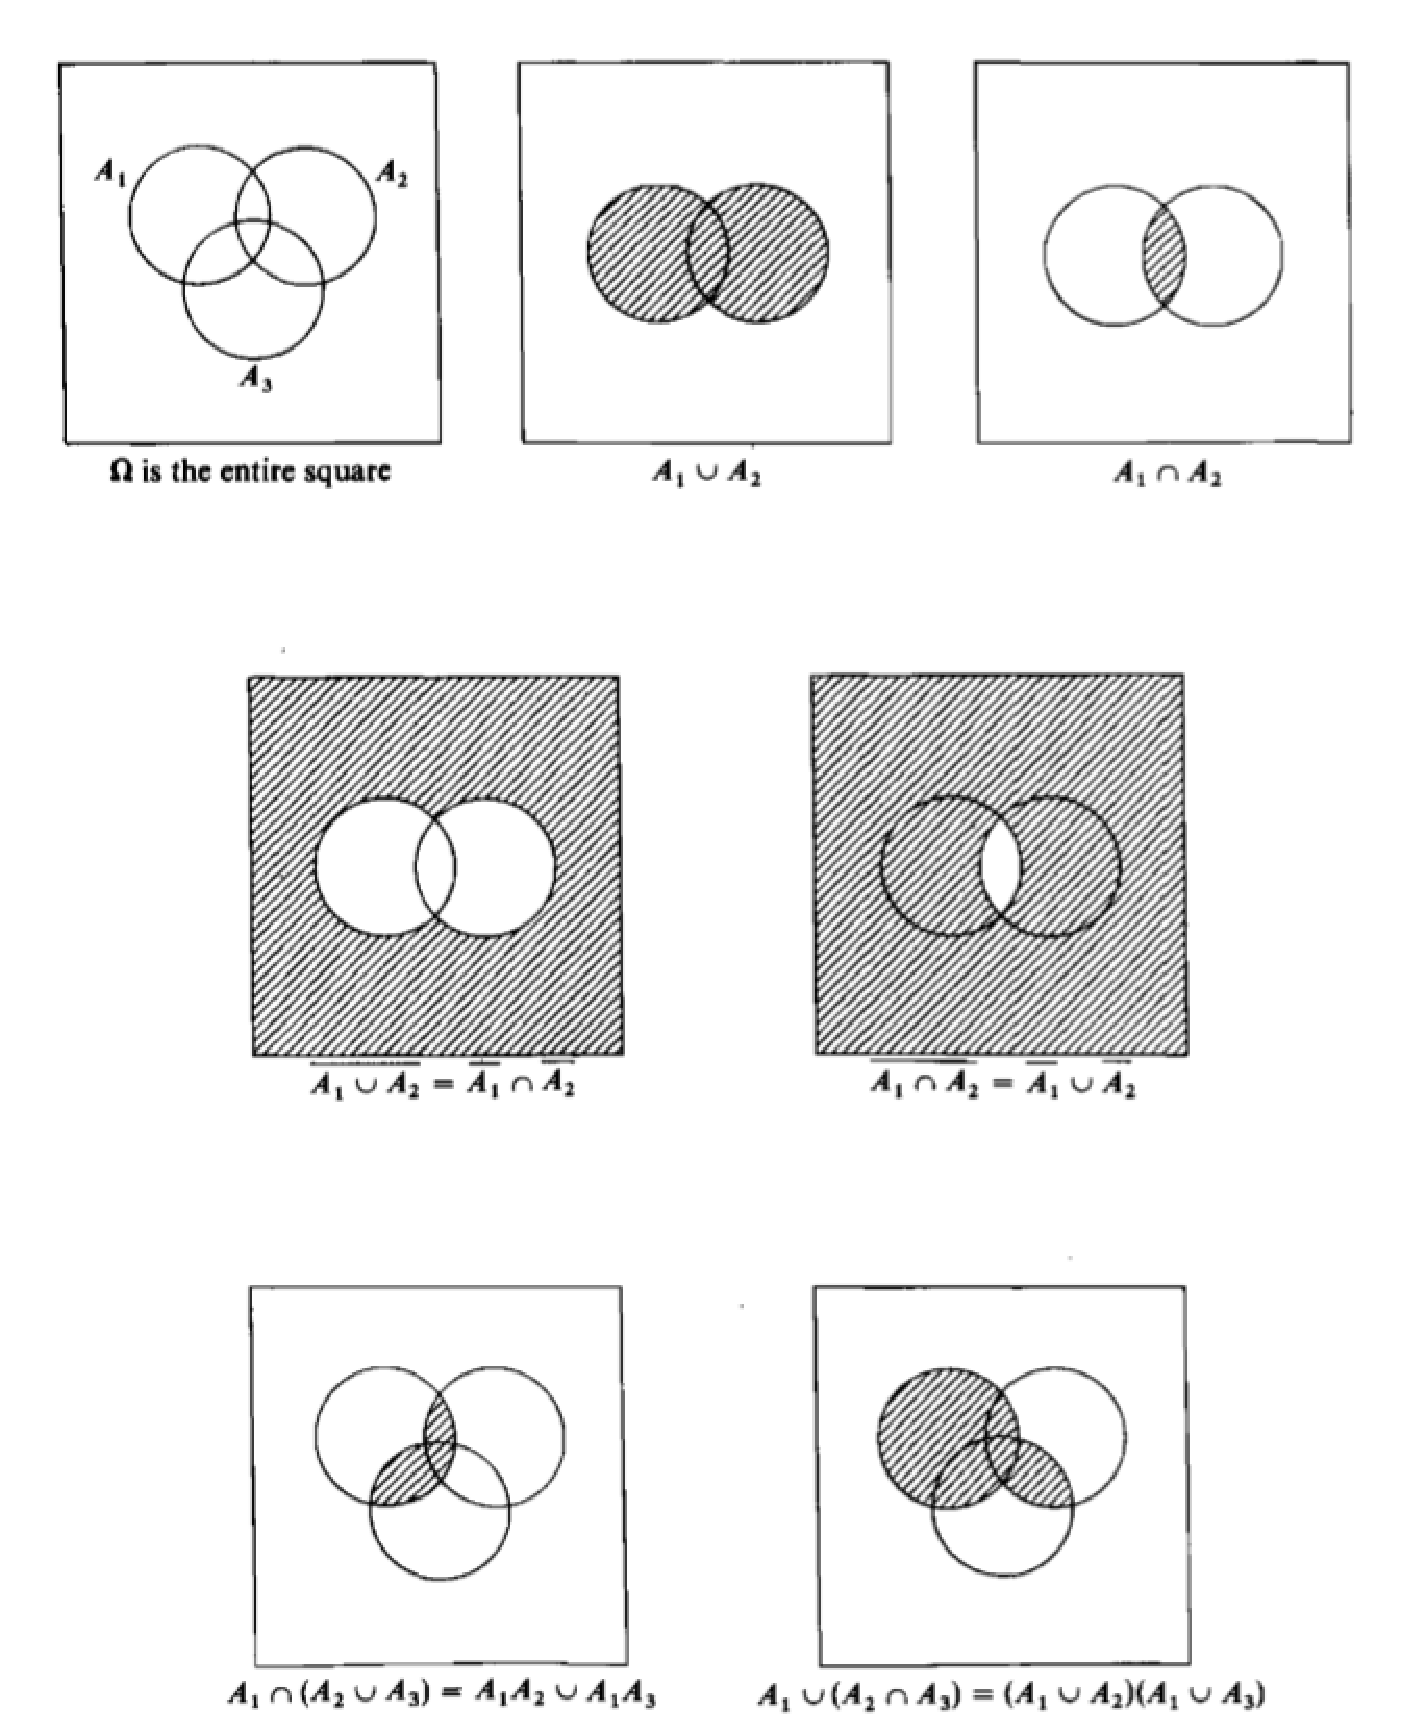
\includegraphics[scale = 0.5]{pictures/set_operations.eps}
\caption{Množinové operace nad náhodnými jevy}
\label{set_operations}
\end{figure} 

Je zvykem rozlišovat jednotlivé množiny v v poli $\Omega$ přiřazením indexů. Označme množinu takovýchto indexů jako $\Lambda$. Jestliže bychom uvažovali pouze dvě podmnožiny pole $\Omega$, pak bude $\Lambda$ obsahovat pouze dva indexy, řekněme $\Lambda = {1, 2}$.

\begin{definition} [Sjednocení a průnik množin]
Nechť $\Lambda$  je množinou indexů a $\{A_{\lambda}: \lambda \in \Lambda\} = \{A_{\lambda}\}$ je souborem podmnožin pole $\Omega$ indexovaných dle $\Lambda$. Množinu, která obsahuje všechny prvky náležící do alespoň jednoho $A_{\lambda}$, nazýváme sjednocením množin $\{A_{\lambda}\}$ a značíme jako $\bigcup_{\lambda \in \Lambda} A_{\lambda}$. Množinu, která obsahuje všechny prvky současně náležících do všech $A_{\lambda}$, nazýváme průnikem množin $\{A_{\lambda}\}$ a značíme jako $\bigcap_{\lambda \in \Lambda} A_{\lambda}$. Jestliže je $\Lambda$ prázdnou množinou, pak definujeme sjednocení jako $\bigcup_{\lambda \in \Lambda} A_{\lambda} = \emptyset$ a průnik jako $\bigcap_{\lambda \in \Lambda} A_{\lambda} = \Omega$.
\end{definition}

\begin{theorem}[De Morganův theorém]
Nechť $\Lambda$ představuje množinu indexů a $\{A_{\lambda}\}$ je souborem všech podmnožin pole $\Omega$ indexovaných dle $\Lambda$. Pak
\begin{equation*}
\Big(\bigcup_{\lambda \in \Lambda} A_{\lambda}\Big)^c = \bigcap_{\lambda \in \Lambda} A^c_{\lambda}
\end{equation*}
\begin{equation*}
\Big(\bigcap_{\lambda \in \Lambda} A_{\lambda}\Big)^c = \bigcup_{\lambda \in \Lambda} A^c_{\lambda}
\end{equation*}
\end{theorem}

\begin{definition}[Disjuktní množiny]
Podmnožiny $A$ a $B$ pole $\Omega$ jsou disjuktní, jestliže $A \cap B = \emptyset$. Podmnožiny $A_1$, $A_2, ...$ jsou vzájemně disjuktní, jestliže $A_i \cap A_j = \emptyset$ pro všechna $i \not= j$.  
\end{definition}

\begin{theorem}
Jestliže jsou $A$ a $B$ podmnožiny pole $\Omega$, pak
\begin{enumerate}
\item $A = (A \cap B) \cup (A \cap B^c)$
\item $(A \cap B) \cap (A \cap B^c) = \emptyset$
\end{enumerate}
\end{theorem}

\begin{proof}
~
\begin{enumerate}
\item $A = A \cap \Omega = A \cap (B \cup B^c) = (A \cap B) \cup (A \cap B^c)$
\item $(A \cap B) \cap (A \cap B^c) = (A \cap A) \cap (B \cap B^c) = A \cap \emptyset = \emptyset$
\end{enumerate}
\end{proof}
\begin{theorem}
Jestliže $A \subset B$, pak $A \cap B = A$ a $A \cup B = B$.
\end{theorem}

\subsection{Definice výběrového prostoru a náhodného jevu}

\begin{definition}[Výběrový prostor]
Výběrový prostor, označovaný jako $\Omega$, představuje soubor všech možných výstupů náhodného experimentu.
\end{definition}

\begin{definition}[Náhodný jev a jevové pole]
Náhodný jev je podmnožinou výběrového prostoru. Množina všech náhodných jevů souvisejících s daným experimentem pak představuje jevové pole tohoto experimentu.
\end{definition}

Výše uvedená definice přesně nevymezuje pojem ``náhodný jev''. Náhodný jev je vždy podmnožinou výběrového prostoru, avšak pro dostatečně velký výběrový prostor ne všechny jeho podmnožiny musí představovat náhodný jev. Proto soubor všech podmnožin výběrového prostoru nemusí nutně odpovídat jevovému poli. Nicméně množina všech náhodných jevů může být vždy zvolena dostatečně velká na to, aby obsahovala všechny náhodné jevy, jejichž pravděpodobností bychom se mohli chtít zabývat. Jestliže se výběrový prostor skládá z konečného počtu prvků, pak odpovídající jevové pole bude množinou všech podmnožin výběrového prostoru.

Naším primárním zájmem je pravděpodobnost, s jakou určitý náhodný jev nastane popř. nenastane. Náhodný jev $A$ nastane, jestliže výsledek experimentu (tj. prvek odpovídajícího výběrového prostoru) náleží $A$. Protože prvek $\omega$ výběrového prostoru $\Omega$ je z definice jeho podmnožinou, je zároveň kandidátem pro náhodný jev. Proto můžeme na $\omega$ nahlížet jako na prvek i jako na podmnožinu $\Omega$. Abychom tyto dva možné pohledy odlišili, používáme značení $\omega$, jestliže mluvíme o prvku, a značení $\{\omega\}$, jestliže mluvíme o podmnožině. Také $\emptyset$ a $\Omega$  jsou podmnožinami $\Omega$ a jsou tak náhodnými jevy. $\Omega$ někdy nazýváme jistým jevem.

Pro značení náhodných jevů se zpravidla používají velká písmena latinské abecedy (s výjimkou výše zmíněných $\emptyset$ a $\Omega$), tj. např. $A$. Jevové pole je pak nejčastěji označeno skriptovým písmenem latinské abecedy jako např. $\mathscr{A}$.

Jevové pole $\mathscr{A}$ by mělo splňovat
\begin{enumerate}
\item $\Omega \in \mathscr{A}$,
\item je-li $A \in \mathscr{A}$, pak $A^c \in \mathscr{A}$ a
\item jestliže $A_1 \in \mathscr{A}$ a $A_2 \in \mathscr{A}$, pak $A_1 \cup A_2 \in \mathscr{A}$.
\end{enumerate}
Jakýkoliv souhrn náhodných jevů, které splňují výše uvedené tři podmnínky, nazýváme algebrou náhodných jevů, zkráceně též algebrou. Je zřejmé, že soubor všech podmnožin výběrového prostoru $\Omega$ splňuje tyto podmínky. Tyto požadované vlastnosti pak implikují následující vlastnosti jevového pole $\mathscr{A}$.

\begin{theorem}
$\emptyset \in \mathscr{A}$
\end{theorem}
\begin{proof}
Uvažujme vlastnost (1) $\Omega \in \mathscr{A}$ a související vlastnost (2) $\Omega^c \in \mathscr{A}$. Nicméně $\Omega^c = \emptyset$, a proto $\emptyset \in \mathscr{A}$.
\end{proof}
\begin{theorem}
Jestliže $A_1 \in \mathscr{A}$ a $A_2 \in \mathscr{A}$, pak $A_1 \cap A_2 \in \mathscr{A}$.
\end{theorem}
\begin{proof}
Platí $A_1^c \in \mathscr{A}$ a $A_2^c \in \mathscr{A}$, což implikuje $A_1^c \cup A_2^c \in \mathscr{A}$ a $(A_1^c \cup A_2^c)^c \in \mathscr{A}$. Zároveň, dle De Morganova pravidla, platí $(A_1^c \cup A_2^c)^c = A_1^c \cap A_2^c = A_1 \cap A_2$.
\end{proof}
\begin{theorem}
Jestliže $A_1, A_2, ..., A_n \in \mathscr{A}$, pak $\cup^{n}_{i=1}A_i \in \mathscr{A}$ a $\cap^{n}_{i=1}A_i \in \mathscr{A}$.
\end{theorem}
V následujícím textu budeme vždy předpokládat, že souhrn všech jevů $\mathscr{A}$ je algebra. V praxi lze algebru $\mathscr{A}$ vytvořit tak, že soubor jevů, o které se zajímáme, rozšíříme o
\begin{enumerate}
\item jistý jev,
\item všechny komplementární jevy a
\item a všechna konečná sjednocení a průniky těchto jevů.
\end{enumerate}
Až dosud jsme nevysvětlili, proč $\mathscr{A}$ není vždy souborem všech podmnožin výběrového prostoru $\Omega$. Vysvětlení poskytneme v následující kapitole.

\subsection{Definice pravděpodobnosti}

\begin{definition}[Funkce]
Funkce $f(\cdot)$ s definičním oborem $A$ a oborem hodnot $B$ je souborem uspořádaných párů $(a, b)$, které splňují
\begin{enumerate}
\item $a \in A$ a $b \in B$,
\item pro každé $a \in A$ existuje uspořádaný pár $(a, b)$\footnote{Obrácené tvrzení však neplatí. Nelze tedy říci, že pro každé $b \in B$ existuje uspořádaný pár $(a, b)$.} a
\item žádné dva uspořádané páry nemají shodný první element\footnote{To znamená, že neexistují dvě uspořádané dvojice $(a, b_1)$ a $(a, b_2)$, kde $b_1 \not= b_2$.}.
\end{enumerate}
\end{definition}

Jestliže $(a, b) \in f(\cdot)$, píšeme $b = f(a)$ a $f(a)$ nazýváme hodnotou funkce $f(\cdot)$ v bodě $a$. Pro libovolné $a \in A$ platí $f(a) \in B$. Označením $f(\cdot)$ rozumíme uspořádaný pár $(a, b = f(a))$. $f(a)$ někdy také nazýváme obrazem bodu $a$ pro $f(\cdot)$.

\begin{definition}[Indikační funkce]
Nechť $\Omega$ představuje prostor s body $\omega$ a $A$ představuje libovolnou podmnožinu $\Omega$. Indikační funkce $A$, označována jako $I_A(\cdot)$, je funkcí s definičním oborem $\Omega$ a oborem hodnot $\{0, 1\}$ a je definována jako
\begin{equation*}
I_A(\omega) = 
\begin{cases}
1~~~\textit{pro}~\omega \in A \\
0~~~\textit{pro}~\omega \notin A
\end{cases}
\end{equation*}
\end{definition}

Nechť $\Omega$ představuje libovolný výběrový prostor a $\mathscr{A}$ libovolný soubor podmnožin $\Omega$. Pak
\begin{enumerate}
\item $I_A(\omega) = 1 - I_{A^c}(\omega)$ pro všechna $A \in \mathscr{A}$,
\item $I_{A_1 \cap A_2 \cap \cdots \cap A_n}(\omega) = I_{A_1}(\omega) \cdot I_{A_2}(\omega) \cdots I_{A_n}(\omega)$ pro $A_1, A_2, ..., A_n \in \mathscr{A}$,
\item $I_{A_1 \cup A_2 \cup \cdots \cup A_n}(\omega) = \max[I_{A_1}(\omega), I_{A_2}(\omega), ..., I_{A_n}(\omega)]$ pro $A_1, A_2, ..., A_n \in \mathscr{A}$ a
\item $I^2_A(\omega) = I_A(\omega)$ pro všechna $A \in \mathscr{A}$.
\end{enumerate}

Indikační funkci lze použít také pro ``indikaci'' podmnožin reálné osy
\begin{equation*}
I_{[0,1]}(x) =
\begin{cases}
1~~~\textit{pro}~ 0 \le x < 1\\
0~~~\textit{v ostatních případech}
\end{cases}
\end{equation*}
popř. množiny přirozených čísel
\begin{equation*}
I_{I^+}(x) =
\begin{cases}
1~~~\textit{jestliže $x$ je přirozené číslo}\\
0~~~\textit{v ostatních případech}
\end{cases}
\end{equation*}

Pro následujicí text předpokládáme, že $\Omega$ označuje výběrový prostor a $\mathscr{A}$ označuje souhrn jevů, které představují algebru pro určitý náhodný experiment.

\begin{definition}[Pravděpodobnostní funkce]
Pravděpodobnostní funkce $P[\cdot]$ je funkcí s definičním oborem $\mathscr{A}$ a oborem hodnot $[0, 1]$, která splňuje axiomy
\begin{enumerate}
\item $P[A] \ge 0$ pro každé $A \in \mathscr{A}$,
\item $P[\Omega] = 1$ a
\item jsou-li $A_1, A_2, ...$ vzájemně neslučitelné jevy\footnote{Jevy $A_i$ a $A_j$ jsou vzájmně neslučitelné, jestliže nemohou nastat současně, tj. $A_i \cap A_j = \emptyset$ pro $i \not= j$.} v $\mathscr{A}$ a jestliže $A_1 \cup A_2 \cup \cdots = \cup_{i=1}^{\infty}A_i \in \mathscr{A}$, pak $P[\cup_{i=1}^{\infty}A_i] = \sum_{i=1}^{\infty}P[A_i]$.
\end{enumerate}
\end{definition}

V naší definici náhodného jevu a jevového pole $\mathscr{A}$ jsme zmínili, že $\mathscr{A}$ nemůže být vždy chápáno jako souhrn všech podmnožin $\Omega$. Důvodem je skutečnost, že pro ``dostatečně velké'' $\Omega$ je soubor všech podmnožin v $\Omega$ příliš velký a je tak nemožné definovat pravděpodobnostní funkci, která by byla konzistentní s výše uvedenými axiomy. Tyto axiomy implikují následující věty.

\begin{theorem}
$P[\emptyset] = 0$
\end{theorem}
\begin{proof}
Uvažujme $A_1 = \emptyset$, $A_2 = \emptyset, ...$. Pak dle axiomu (3) platí
\begin{equation*}
P[\emptyset] = P[\cup_{i=1}^{\infty}A_i] = \sum_{i=1}^{\infty}P[A_i] = \sum_{i = 1}^{\infty}P[\emptyset]
\end{equation*}
což platí, pouze je-li $P[\emptyset] = 0$.
\end{proof}
\begin{theorem}
Jestliže jsou $A_1, ..., A_n$ vzájemně neslučitelné jevy v $\mathscr{A}$, pak
\begin{equation*}
P[A_1 \cup \cdots \cup A_n] = \sum_{i=1}^n P[A_i]
\end{equation*}
\end{theorem}
\begin{proof}
Nechť $A_{n+1} = \emptyset, A_{n+2} = \emptyset, ...$. Pak $\cup_{i = 1}^nA_i = \cup_{i = 1}^{\infty}A_i \in \mathscr{A}$ a
\begin{equation*}
P[\cup_{i=1}^n A_i] = P[\cup_{i=1}^{\infty}A_i] = \sum_{i=1}^{\infty}P[A_i] = \sum_{i=1}^nP[A_i]
\end{equation*}
\end{proof}
\begin{theorem}
Jestliže je $A$ jevem z jevového pole $\mathscr{A}$, pak
\begin{equation*}
P[A^c] = 1 - P[A]
\end{equation*}
\end{theorem}
\begin{proof}
$A \cup A^c = \Omega$ a $A \cap A^c = \emptyset$. Proto
\begin{equation*}
P[\Omega] = P[A \cup A^c] = P[A] + P[A^c]
\end{equation*}
Zároveň však platí $P[\Omega] = 1$, čímž jsme dokázali požadované.
\end{proof}
\begin{theorem}
Jestliže $A \in \mathscr{A}$ a $B \in \mathscr{A}$, pak
\begin{equation*}
P[A] = P[A \cap B] + P[A \cap B^c]
\end{equation*}
a
\begin{equation*}
P[A-B] = P[A \cap B^c] = P[A] - P[A \cap B]
\end{equation*}
\end{theorem}
\begin{proof}
$A = A \cap B \cup A \cap B^c$ a $(A \cap B) \cup (A \cap B^c) = \emptyset$. Proto $P[A] = P[A \cap B] + P[A \cap B^c]$.
\end{proof}
\begin{theorem}
Pro každé dva jevy $A \in \mathscr{A}$ a $B \in \mathscr{A}$ platí $P[A \cap B] = P[A] + P[B] - P[A \cap B]$. Tuto větu lze zobecnit do tvaru
\begin{gather*}
P[A_1 \cup A_2 \cup \cdots \cup A_n] = \sum_{j=1}^n P[A_j] - \sum \sum_{i<j}P[A_i \cap A_j] + \\ +\sum \sum \sum_{i<j<k}P[A_i \cap A_j \cap A_k] - \cdots + (-1)^{n+1}P[A_1 \cap A_2 \cap \cdots \cap A_n]
\end{gather*}
\end{theorem}
\begin{proof}
Platí $A \cup B = A \cup (A^c \cap B)$ a $A \cap (A^c \cap B) = \emptyset$. Proto
\begin{equation*}
P[A \cup B] = P[A] + P[A^c \cap B] = P[A] + P[B] - P[A \cap B]
\end{equation*}
Zobecněnou verzi věty lze dokázat pomocí indukce.
\end{proof}
\begin{theorem}
Jestliže $A \in \mathscr{A}$ a $B \in \mathscr{A}$ a $A \subset B$, pak $P[A] \le P[B]$.
\end{theorem}
\begin{proof}
Platí $B = (B \cap A) \cup (B \cap A^c)$ a $A = B \cap A$. Proto $B = A \cup (B \cap A^c)$ a $A \cap (B \cap A^c) = \emptyset$, což implikuje $P[B]=P[A]+P[B \cap A^c]$. Důkaz završíme zjištěním, že $P[B \cap A^c] \ge 0$.
\end{proof}
\begin{theorem}[Booleova nerovnost]
Jestliže $A_1, A_2, ..., A_n \in \mathscr{A}$, pak
\begin{equation*}
P[A_1 \cup A_2 \cup \cdots \cup A_n] \le P[A_1] + P[A_2] + \cdots + P[A_n]
\end{equation*}
\end{theorem}
\begin{proof}
Platí $P[A_1 \cup A_2] = P[A_1] + P[A_2] - P[A_1 \cap A_2] \le P[A_1] + P[A_2]$. Důkaz lze dokončit pomocí indukce.
\end{proof}
\begin{definition}[Pravděpodobnostní prostor]
Pravděpodobnostní prostor je definován tripletem $(\Omega, \mathscr{A}, P[\cdot])$, kde $\Omega$ představuje výběrový prostor, $\mathscr{A}$ jevové pole a $P[\cdot]$ pravděpodobnostní funkci s definičním oborem $\mathscr{A}$.
\end{definition}

\subsection{Konečný výběrový prostor}

Nechť $\omega_1, \omega_2, ..., \omega_n$ představují elemetární jevy konečného výběrového prostoru $\Omega$. Uvažujme funkci $P[\cdot]$ s definičním oborem tvořeným souborem všech podmnožin prostoru $\Omega$, která splňuje následující podmínky
\begin{enumerate}
\item $P[\{\omega_1\}] = P[\{\omega_2\}] = \cdots = P[\{\omega_N\}]$
\item Je-li $A$ podmnožinou $\Omega$ obsahující $N(A)$ elementárních jevů, pak $P[A] = N(A)/N$.
\end{enumerate}
Lze relativně snadno dokázat, že funkce $P[\cdot]$ splňuje všechny tři axiomy kladené na pravděpodobnostní funkce, a proto je pravděpodobnostní funkcí.

\begin{definition}[Pravděpodobnostní funkce se shodnou pravděpodobností]
Pravděpodobnostní funkce $P[\cdot]$, která splňuje výše uvedené dvě podmínky, je tzv. pravděpodobnostní funkcí se shodnou pravděpodobností.
\end{definition}

Uvažujme experiment, jehož výsledkem je vzorek o velikosti $n$. Myšlenku lze ilustrovat na příkladu nádoby obsahující $M$ míčků, ze které je náhodně taženo $n$ míčků. Existují dva základní způsoby výběru vzorku a to s vracením (po té, co je míček vybrán, je vrácen zpět do nádoby) a bez vracení (po té, co je míček vybrán, je odložen stranou). Jestliže bude záležet na pořadí, v jakém jsou míčky taženy, pak v případě náhodného výběru s vracením existuje $M^n = \underbrace{M \cdots M}_n$ a v případě náhodného výběru bez vracení $(M)_n = M(M - 1) \cdots (M - n + 1)$ $n$-tic. Jestliže na pořadí, v jakém jsou míčky taženy, nezáleží, existuje v případě výběru s vracením $\frac{M^n}{n!}$ a v případě výběru bez vracení $\binom{M}{n} = \frac{(M)_n}{n!}$ $n$-tic. $n$-tice, u kterých záleží na pořadí, nazýváme uspořádané, a $n$-tice, u kterých na pořadí nezáleží, nazýváme neuspořádané.

\begin{example}
Uvažujme množinu $S$ o $M$ prvcích. Celkový počet podmnožin množiny $S$ je roven $\sum_{n = 0}^M \binom{M}{n}$. Pro  $a = b = 1$ je z binomické věty $(a + b)^M = \sum_{n=0}^M \binom{M}{n}a^nb^{M-n}$ zřejmé, že $2^M = \sum_{n=0}^M \binom{M}{n}$. Množina o $M$ prvcích tak má $2^M$ podmnožin.
\end{example}

Uvažujme situaci, kdy nádoba obsahuje $M$ míčků, z nichž právě $K$ je bílých. Pravděpodobnost, že při výběru $n$ míčků s vracením jich bude právě $k$ bílých, je rovna
\begin{equation*}
\frac{\binom{n}{k}K^k(M-K)^{n-k}}{M^n}
\end{equation*}
Pří výběru bez vracení je tato pravděpodobnosti rovna
\begin{equation*}
\frac{\binom{n}{k}(K)_k(M-K)_{n-k}}{(M)_n} = \frac{\binom{K}{k}\binom{M-K}{n-k}}{\binom{M}{n}}
\end{equation*}
Pro úplnost dodejme, že v kontextu výše uvedených dvou rovnic je pořadí, v jakém jsou míčky taženy, irelevantní.

Až dosud jsme uvažovali, že pravděpodobnost realizace jednotlivých výsledků náhodného experimentu jsou shodné. V řadě případů však tento předpoklad nemusí být splněn. Nechť $\Omega = \{\omega_1, ..., \omega_2\}$ a předpokládejme $p_j = P[\{ \omega_j\}]$ pro $j = 1, ..., N$. Proto
\begin{equation*}
1 = P[\Omega] = P \big[\cup_{j=1}^N \{\omega_j \} \big] = \sum_{j = 1}^N P[\{ \omega_j \}] = \sum_{j = 1}^N p_j
\end{equation*}
Pro libovolný jev $A$ pak definujeme $P[A] = \sum p_j$, kde sumace jde přes ta $\omega_j$, která náleží $A$. Lze dokázat, že takto definovaná $P[\cdot]$ splňuje všechny tři axiomy pravděpodobnostní funce, a proto je pravděpodobnostní funkcí.

\subsection{Podmíněná pravděpodobnost a nezávislost}

\begin{definition}[Podmíněná pravděpodobnost]
Nechť $A$ a $B$ jsou dva jevy z $\mathscr{A}$ pro pravděpodobnostní prostor $(\Omega, \mathscr{A}, P[\cdot])$. Podmíněná pravděpodobnost jevu $A$ za předpokladu realizace jevu $B$ je definována jako
\begin{equation*}
P[A|B] = \frac{P[A \cap B]}{P[B]}~~~\textit{pro}~P[B] > 0
\end{equation*}
V případě $P[B] = 0$ není tato pravděpodobnost definována. 
\end{definition}
Z výše uvedeného je zřejmé, že $P[A \cap B] = P[A|B]P[B] = P[B|A]P[A]$ pro $P[A] > 0$ a $P[B] > 0$. Tato rovnice tak definuje vztah mezi $P[A|B]$ a $P[B|A]$ na základě nepodmíněných pravděpodobností $P[A]$ a $P[B]$.

Výše uvedená definice je v konsistentní s klasickou definicí pravděpodobnosti. Jestliže máme náhodný experiment, pro který jsou definovány jevy $A$ a $B$, lze $P[A|B]$ definovat jako
\begin{equation*}
P[A|B] = \frac{N_{AB}}{N_B}
\end{equation*}
kde $N_B$ představuje počet realizací jevu $B$ a $N_{AB}$ představuje počet realizací jevu $A \cap B$. Je-li celkový počet realizací $N$, platí totiž
\begin{equation*}
P[A|B] = \frac{P[A \cap B]}{P[B]} = \frac{N_{AB}/N}{N_B/N} = \frac{N_{AB}}{N_B}
\end{equation*}

Když mluvíme o podmíněné pravděpodobnosti, podmiňujeme vzhledem k určitému jevu $B$ (tj. předpokládáme, že výstup náhodného experimentu je $B$). Náhodný jev $B$ se tak stává novým výběrovým prostorem. Vyvstává otázka, zda-li je $P[\cdot | B]$ pravděpodobnostní funkcí s definičním oborem $\mathscr{A}$, tj. zda-li splňuje tři axiomy pravděpodobnostní funkce.
\begin{enumerate}
\item $P[A|B] = P[A \cap B] / P[B] \ge 0 ~~~\textit{pro všechna}~A \in \mathscr{A}$
\item $P[\Omega|B] = P[\Omega \cap B] / P[B] = P[B] / P[B] = 1$
\item Je-li $A_1, A_2, ...$ posloupností vzájemně neslučitelných jevů v $\mathscr{A}$ a $\cup_{i=1}^{\infty}A_i \in \mathscr{A}$, pak
\begin{equation*}
P\Big[ \cup_{i=1}^{\infty}A_i|B\Big] = \frac{P\Big[ \Big(\bigcup_{i=1}^{\infty}A_i \Big)B\Big]}{P[B]} = \frac{P \Big[ \bigcup_{i=1}^{\infty}(A_i \cap B)\Big]}{P[B]} = \frac{\sum_{i=1}^{\infty}P[A_i \cap B]}{P[B]} = \sum_{i=1}^{\infty}P[A_i|B]
\end{equation*}
\end{enumerate}
Následující věty jsou analogií vět z kapitoly (1.2.4).
\begin{theorem}
$P[\emptyset | B] = 0$
\end{theorem}
\begin{theorem}
Jsou-li $A_1, ..., A_n$ vzájemně neslučitelné jevy v $\mathscr{A}$, pak $P[A_1 \cup \cdots \cup A_n | B] = \sum_{i=1}^nP[A_i|B]$.
\end{theorem}
\begin{theorem}
Jestliže $A$ jevem v $\mathscr{A}$, pak $P[A^c|B] = 1 - P[A|B]$.
\end{theorem}
\begin{theorem}
Jestliže $A_1 \in \mathscr{A}$ a $A_2 \in \mathscr{A}$, pak $P[A_1|B] = P[A_1 \cap A_2|B] + P[A_1 \cap A_2^c|B]$.
\end{theorem}
\begin{theorem}
Pro každé dva jevy $A_1 \in \mathscr{A}$ a $A_2 \in \mathscr{A}$ platí $P[A_1 \cup A_2|B] = P[A_1|B] + P[A_2|B] - P[A_1 \cap A_2|B]$
\end{theorem}
\begin{theorem}
Jestliže $A_1 \in \mathscr{A}$, $A_2 \in \mathscr{A}$ a $A_1 \subset A_2$, pak $P[A_1|B] \le P[A_2|B]$.
\end{theorem}
\begin{theorem}
Jestliže $A_1, A_2, ..., A_n \in \mathscr{A}$, pak $P[A_1 \cup A_2 \cup \cdots \cup A_n | B] \le \sum_{i=1}^n P[A_i|B]$.
\end{theorem}
\begin{theorem}[Celková pravděpodobnost]
Jestliže pro daný pravděpodobnostní prostor $(\Omega, \mathscr{A}, P[\cdot])$ představuje $B_1, B_2, ..., B_n$ soubor vzájemně neslučitelných jevů v $\mathscr{A}$ splňujících podmínky $\Omega = \bigcup_{j=1}^n B_j$ a $P[B_j] > 0$ pro $j = 1, ..., n$, pak pro každé $A \in \mathscr{A}$ platí $P[A] = \sum_{j=1}^nP[A|B_j]P[B_j]$.
\end{theorem}
\begin{proof}
Všimněme si, že $A = \bigcup_{j=1}^n (A \cap B_j)$ a že jednotlivé $A \cap B_j$ jsou vzájemně neslučitelné. Proto
\begin{equation*}
P[A] = P\Big[\bigcup_{j=1}^n (A \cap B_j)\Big] = \sum_{j=1}^nP[A \cap B_j] = \sum_{j=1}^n P[A|B_j]P[B_j]
\end{equation*}
\end{proof}
\begin{corollary}
Uvažujme pravděpodobnostní prostor $(\Omega, \mathscr{A}, P[\cdot])$. Nechť $B \in \mathscr{A}$ splňuje $0 < P[B] < 1$. Pak pro každé $A \in \mathscr{A}$ platí $P[A] = P[A|B]P[B]+P[A|B^c]P[B^c]$
\end{corollary}

\begin{theorem} [Bayesův vzorec]
Uvažujme pravděpodobnostní prostor $(\Omega, \mathscr{A}, P[\cdot])$ a soubor vzájemně neslučitelných jevů $B_1, B_2, ..., B_n$ v $\mathscr{A}$. Nechť tyto jevy splňují podmínky $\Omega = \bigcup_{j=1}^n B_j$ a $P[B_j] > 0$ pro $j = 1, 2, ..., n$. Pak pro každé $A \in \mathscr{A}$, které splňuje  $P[A] > 0$, platí
\begin{equation*}
P[B_k|A]=\frac{P[A|B_k]P[B_k]}{\sum_{j=1}^nP[A|B_j]P[B_j]}
\end{equation*}
\begin{proof}
S využitím definice podmíněné pravděpodobnosti a větě o celkové pravděpodobnosti lze dokázat, že
\begin{equation*}
P[B_k|A]=\frac{P[B_k \cap A]}{P[A]} = \frac{P[A|B_k]P[B_k]}{\sum_{j=1}^nP[A|B_j]P[B_j]}
\end{equation*}
\end{proof}
\end{theorem}
\begin{corollary}
Pro daný pravděpodobnostní prostor $(\Omega, \mathscr{A},P[\cdot])$ uvažujme takové jevy $A \in \mathscr{A}$ a $B \in \mathscr{A}$, které splňují $P[A] > 0$ a $0 < P[B] < 1$. Pak platí
\begin{equation*}
P[B|A] = \frac{P[A|B]P[B]}{P[A|B]P[B]+P[A|B^c]P[B^c]}
\end{equation*}
\end{corollary}
\begin{theorem}[Pravidlo multiplikace]
Pro daný pravděpodobnostní prostor $(\Omega, \mathscr{A}, P[\cdot])$ uvažujme jevy $A_1, A_2, ..., A_n$ náležící do $\mathscr{A}$, pro které $P[A_1 \cap \cdots \cap A_2] > 0$. Pak
\begin{equation*}
P[A_1 \cap \cdots \cap A_n] = P[A_1]P[A_2|A_1]P[A_3| A_1 \cap A_2] \cdots P[A_n|A_1 \cap \cdots \cap A_{n-1}]
\end{equation*}
\end{theorem}
\begin{theorem}[Nezávislé jevy]
Pro daný pravděpodobnostní prostor $(\Omega, \mathscr{A}, P[\cdot])$ uvažujme náhodné jevy $A \in \mathscr{A}$ a $B \in \mathscr{A}$. Jevy $A$ a $B$ jsou nezávislé tehdy a jen tehdy, jestliže je splněna některá z následujících ekvivalentních podmínek.
\begin{enumerate}
\item $P[A \cap B] = P[A]P[B]$
\item $P[A | B] = P[A]$ jestliže $P[B] > 0$
\item $P[B | A] = P[B]$ jestliže $P[A] > 0$
\end{enumerate}
\end{theorem}
Abychom dokázali, že všechny tři výše uvedené podmínky jsou ekvivalentní, stačí dokázat, že (1) implikuje (2), (2) implikuje (3) a (3) implikuje (1). Jestliže $P[A \cap B] = P[A]P[B]$, pak $P[A|B] = P[A \cap B] / P[B] = P[A]P[B]/P[B] = P[A]$ pro $P[B] > 0$. Z toho plyne, že (1) implikuje (2). Jestliže $P[A|B] = P[A]$, pak $P[B|A]=P[A|B]P[B]/P[A]=P[A]P[B]/P[A]=P[B]$ pro $P[A]>0$ a $P[B]>0$. Z toho plyne, že (2) implikuje (3). Jestliže $P[B|A]=P[B]$, pak $P[A \cap B] = P[B|A]P[A] = P[B]P[A]$ pro $P[A]>0$. Je tedy zřejmé, že $P[A \cap B] = P[A]P[B]$, jestliže $P[A] = 0$ nebo $P[B]=0$.

Nezávislost a neslučitelnost jevů $A$ a $B$ jsou dva rozdílné pojmy. Např. dva vzájemně neslučitelné jevy $A$ a $B$ jsou nezávislé tehdy a jen tehdy jestliže $P[A]P[B] = 0$. To je splněno tehdy a jen tehdy, jestliže jeden z jevů má nulovou pravděpodobnost. Neboli, jestliže $P[A] \not= 0$ a $P[B] \not= 0$, nezávislost mezi jevy $A$ a $B$ implikuje, že tyto jevy nejsou vzájemně neslučitelné. Analogicky $P[A] \not= 0$ a $P[B] \not= 0$ a neslučitenost jevů $A$ a $B$ implikuje, že se nejedná o nezávislé jevy.

\begin{example}
Uvažujme hod hrací kostkou. Definujme jev $A$ jako situaci, kdy padne sudé číslo a jev $B$ jako situaci, kdy padle liché číslo. Je zřejmé, že tyto jevy jsou neslučitelné, avšak nejsou nezávislé. 
\end{example}

\begin{theorem}
Jestliže jsou $A$ a $B$ dva nezávislé jevy definované na daném pravděpodobnostním prostoru $(\Omega, \mathscr{A}, P[\cdot])$, pak $A$ a $B^c$ jsou nezávislé, $A^c$ a $B$ jsou nezávislé a $A^c$ a $B^c$ jsou nezávislé.
\end{theorem}
\begin{proof}
\begin{equation*}
P[A \cap B^c] = P[A] - P[A \cap B] = P[A] - P[A] P[B] = P[A](1 - P[B]) = P[A]P[B^c] 
\end{equation*}
V ostatních případech je důkaz analogický.
\end{proof}
\begin{definition}[Nezávislost náhodných jevů]
Pro daný pravděpodobnostní prostor $(\Omega, \mathscr{A}, P[\cdot])$ uvažujme náhodné jevy $A_1, A_2, ..., A_n$ v $\mathscr{A}$. Jevy $A_1, A_2, ..., A_n$ jsou nezávislé tehdy a jen tehdy, jestliže
\begin{gather*}
P[A_i \cap A_j] = P[A_i]P[A_j]~~~\textit{pro}~i \not= j\\
P[A_i \cap A_j \cap A_k] = P[A_i]P[A_j]P[A_k]~~~\textit{pro}~i \not= j, j \not= k, i \not= k\\
\cdots\\
P\Big[\bigcap_{i = 1}^n A_i \Big] = \prod_{i=1}^n P[A_i]
\end{gather*}
\end{definition}
Pro nezávislost vícero náhodných jevů je třeba, aby byly splněny všechny podmínky. Nestačí tak např. testovat pouze párovou nezávislost, protože ta sama o sobe nezaručuje vzájemnou nezávislost všech jevů.

\chapter{Náhodné veličiny, distribuční a momentová funkce}

\section{Náhodná veličina a kumulativní distribuční funkce}

\begin{definition}[Náhodná veličina]
Pro daný pravděpodobnostní prostor $(\Omega, \mathscr{A}, P[\cdot])$ je náhodná veličina $X$, označovaná také jako $X(\cdot)$, funkcí s definičním oborem hodnot $\Omega$ a reálnou osou jako oborem hodnot. Funkce $X(\cdot)$ musí splňovat podmínku, že množina $A_r = \{\omega: X(\omega) \le r\}$ náleží do $\mathscr{A}$ pro každé reálné číslo $r$.
\end{definition}
Jestliže tuto definici zasadíme do rámce náhodného experimentu, pak
\begin{enumerate}
\item $\Omega$ je úplným souborem všech možných výsledků tohoto experimentu a
\item náhodná veličina $X(\cdot)$ je funkcí s definičním oborem $\Omega$, která přiřazuje reálné číslo každému výsledku náhodného experimentu.
\end{enumerate}
Požadavek, aby $\omega$, pro které platí $X(\omega) \le r$, bylo náhodným jevem (tj. prvkem $\mathscr{A}$), není nikterak omezující, protože naším záměrem je používat pojmu náhodná veličina pouze k popisu náhodných jevů. Jen zřídka kdy se totiž budeme zajímat o náhodnou veličinu jako takovou - předmětem našeho zájmu budou spíše náhodné jevy definované skrze náhodné veličiny.
V následujícím textu budeme pro označení náhodných veličin používat velkých písmen latinské abecedy (např. $X$) a pro označení jejich konkrétních hodnot pak malých písmen latinské abecedy (např. $X = x$).

\begin{example}
Uvažujme hod mincí. Nechť náhodná veličina $X$ označuje počet hlav. Je zřejmé, že $\Omega = \{\textit{orel, hlava}\}$, $X(\omega) = 1$ pro $\omega = \textit{hlava}$ a $X(\omega) = 0$ jestliže $\omega = \textit{orel}$. Náhodná veličina $X$ tak asociuje reálné čéslo s každým možným výsledkem náhodného experimentu. Měli bychom tedy dokázat, že $\{\omega: X(\omega) \le r\}$ náleží do $\mathscr{A}$ pro každé reálné číslo $r$. V našem případě se $\mathscr{A}$ skládá ze čtyř podmnožin - $\emptyset, \textit{\{hlava\}}, \textit{\{orel\}}$ a $\Omega$. Jestliže $r < 0$, pak $\{\omega: X(\omega) \le r\} = \emptyset$. Jestliže $0 \le r < 1$, pak ${\omega: X(\omega) \le r} = \textit{\{orel\}}$. Jestliže $r \ge 1$, pak $\{\omega: X(\omega)\} = \Omega = \textit{\{hlava, orel\}}$. Proto pro každé $r$ náleží množina $\{\omega: X(\omega) \le r\}$ do $\mathscr{A}$ a $X(\cdot)$ je tak náhodnou veličinou.
\end{example}

\begin{definition}[Kumulativní distribuční funkce]
Kumulativní distribuční funkce $F_X(\cdot)$ náhodné veličiny $X$ je definována jako funkce, jejímž definičním oborem je reálná osa a oborem hodnot je interval $[0, 1]$ a která splňuje podmínku $F_X(x) = P[X \le x] = P[X \le x] = P[\{\omega: X(\omega) \le x\}]$ pro každé reálné číslo $x$.
\end{definition}
Každá náhodná veličina je jedinečně definována skrze svou kumulativní distribuční funkci. S pomocí příslušné kumulativní distribuční funkce a s pomocí definice náhodné veličiny lze nalézt pravděpodobnost daného náhodného jevu\footnote{V tomto případě je využito požadavku, aby $\omega: X(\omega) \le r$ náleželo do $\mathscr{A}$.}.

\begin{example}
Uvažujme hod mincí. Nechť náhodná veličina $X$ označuje počet hlav. Kumulativní distribuční funkce je definována jako
\begin{equation*}
F_X(x) =
\begin{cases}
0~~~\textit{pro}~x<0\\
\frac{1}{2}~~~\textit{pro}~x\le x < 1\\
1~~~\textit{pro}~x\ge 1
\end{cases}
\end{equation*}
popř. s využitím idikační funkcí jako
\begin{equation*}
F_X(x) = \frac{1}{2}I_{[0,1)}(x) + I_{[1, \infty)}(x)
\end{equation*}
\end{example}
\begin{definition}[Vlastnosti kumulativní distribuční funkce]
Z výše uvedeného lze vypozorovat, že kumulativní distribuční funkce má následující vlastnosti.
\begin{enumerate}
\item $F_X(-\infty) \equiv \lim_{x \rightarrow -\infty} F_X(x) = 0$ a $F_X(+\infty) \equiv \lim_{x \rightarrow +\infty} F_X(x) = 1$
\item $F_X(\cdot)$ je monotonní, neklesající funkcí. To znamená, že $F_X(a) \le F_X(b)$ pro $a < b$.
\item $F_X(\cdot)$ je spojitá zprava. To znamená, že $\lim_{0 < h \rightarrow 0} F_X(x + h) = F_X(x)$\footnote{Spojitost zprava je dána definicí $F_X(x) = P[X \le x]$. Pokud bychom, jako někteří jiní autoři, použili definici $F_X(x) = P[X < x]$, pak by $F_X(\cdot)$ byla spojitá zleva.}.
\end{enumerate}
\end{definition}

\begin{proof}
Dokažme vlastnost (2). Platí $\{\omega: X(\omega) \le b\} = \{X \le b \} = \{X \le a \} \cup \{ a < X \le b\}$ a $\{X \le a \} \cap \{a < X \le b\} = \emptyset$. Proto $F_X(b) = P[X \le b] = P[X \le a] + P[a < X \le a] = F_X(a)$.
\end{proof}

\begin{definition}[Kumulativní distribuční funkce]
Libovolná funkce $F(\cdot)$ s reálnou osou jako definičním oborem a oborem hodnot $[0, 1]$, která splňuje všechny tři výše uvedené podmínky, je kumulativní distribuční funkce.
\end{definition}

\section{Pravděpodobnostní funkce}

\subsection{Nespojitá náhodná veličina}

\begin{definition} [Nespojitá náhodná veličina]
Náhodná veličina $X$ je nespojitá, jestliže množina hodnot, kterých může nabývat, je spočetná. Jestliže je náhodná veličina $X$ nespojitá, pak je nespojitá také její kumalativní distribuční funkce $F_X(\cdot)$. Vedle pojmu nespojitá náhodná veličina se někdy používá také pojem diskrétní náhodná veličina.
\end{definition}

Spočetnou množinou rozumíme množinu, která má konečný popř. spočetný počet prvků $x_1, x_2, ...$. Jestliže náhodná veličina $X$ nabývá náhodných hodnot z takovéto množiny, pak $\Omega = \bigcup_n \{\omega: X(\omega) = x_n\} = \bigcup_n \{X = x_n \}$ a $\{X = x_i\} \cap \{X = x_j\} = \emptyset$ pro $i \not= j$. Proto na základě třetího aximu pravděpodobnosti platí $1 = P[\Omega] = \sum_n P[X = x_n]$.

\begin{definition}[Pravděpodobnostní funkce nespojité náhodné veličiny]
Uvažujme náhodnou veličinu $X$, která může nabývat hodnot $x_1, x_2, ..., x_n, ...$. Pak funkce $f_X(\cdot)$ definovaná jako
\begin{equation*}
f_X(x) =
\begin{cases}
P[X = x_j]~~~\textit{pro}~x=x_j, j = 1, 2, ..., n, ...\\
0~~~\textit{pro}~x \not= x_j
\end{cases}
\end{equation*}
je nespojitou pravděpodobnostní funkcí nespojité náhodné veličiny $X$.
\end{definition}

Hodnoty $x_1, x_2, ...$, kterých může nespojitá náhodná veličina $X$ nabývat, nazýváme body koncentrace. Hodnotu pravděpodobnostní funce $f_X(x_j)$ pak nazýváme koncentrací v bodě $x_j$.

\begin{theorem}
Nechť je $X$ nespojitou náhodnou veličinou. Platí, že $F_X(\cdot)$ lze získat z $f_x(\cdot)$ a naopak.
\end{theorem}

\begin{proof}
Označme hodnoty náhodné veličiny $X$ jako $x_1, x_2, ...$.
\begin{enumerate}
\item  Jestliže je dáno $f_X(\cdot)$, pak $F_X(x) = \sum_{j:x_j \le x} f_X(x_j)$.
\item Jestliže je dáno $F_X(x)$, pak $f_X(x_j) = F_X(x_j) - \lim_{h \rightarrow 0^+} F_X(x_j - h)$. $f_X(x_j)$ lze tímto způsobem nalézt pro všechny body koncentrace $x_j$ a $f_X(x) = 0$ pro $x \not= x_j, j = 1, 2, ...$, čímž jsme definovali $f_X(x)$ pro všechna reálná čísla.
\end{enumerate}
\end{proof}

\begin{example}
Uvažujme hod hrací kostkou. Náhodná veličina $X$, která představuje hodnotu hodu, má množinu bodů koncentrace $\{1, 2, 3, 4, 5, 6\}$. Odpovídající nespojitá pravděpodobnostní funkce a kumulativní distribuční funkce jsou pak definovány jako
\begin{equation*}
f_X(x_j) = \frac{1}{6}~~~\textit{pro}~j = 1, 2, ..., 6
\end{equation*}
\begin{equation*}
F_X(x_j) = \frac{j}{6}~~~\textit{pro}~j = 1, 2, ..., 6
\end{equation*}
\end{example}

\figure[h]\centering
\begin{pspicture}(11.0,5.0)
    \psline[arrows=->](0.5,0.5)(5.0,0.5)
    \psline[arrows=->](0.5,0.5)(0.5,4.5)
    \rput(0.0,4.8){\psframebox*{$f_X(x)$}}
    \rput(5.0,0.2){\psframebox*{$x$}}

    \psline[arrows=-*](1.1,0.4)(1.1,1.2)
    \psline[arrows=-*](1.7,0.4)(1.7,1.2)
    \psline[arrows=-*](2.3,0.4)(2.3,1.2)
    \psline[arrows=-*](2.9,0.4)(2.9,1.2)
    \psline[arrows=-*](3.5,0.4)(3.5,1.2)
    \psline[arrows=-*](4.1,0.4)(4.1,1.2)
    \rput(1.1,0.2){\psframebox*{\tiny{1}}}
    \rput(1.7,0.2){\psframebox*{\tiny{2}}}
    \rput(2.3,0.2){\psframebox*{\tiny{3}}}
    \rput(2.9,0.2){\psframebox*{\tiny{4}}}
    \rput(3.5,0.2){\psframebox*{\tiny{5}}}
    \rput(4.1,0.2){\psframebox*{\tiny{6}}}

    \psline[arrows=->](5.5,0.5)(10.5,0.5)
    \psline[arrows=->](5.5,0.5)(5.5,4.5)
    \rput(5.0,4.8){\psframebox*{$F_X(x)$}}
    \rput(10.5,0.2){\psframebox*{$x$}}

    \psline[arrows=*-o](6.1,1.2)(6.8,1.2)
    \psline[arrows=*-o](6.8,1.9)(7.5,1.9)
    \psline[arrows=*-o](7.5,2.6)(8.2,2.6)
    \psline[arrows=*-o](8.2,3.3)(8.9,3.3)
    \psline[arrows=*-o](8.9,3.9)(9.6,3.9)
    \psline[arrows=*-o](9.6,4.5)(10.3,4.5)
    \psline(6.1,0.4)(6.1,0.6)
    \psline(6.8,0.4)(6.8,0.6)
    \psline(7.5,0.4)(7.5,0.6)
    \psline(8.2,0.4)(8.2,0.6)
    \psline(8.9,0.4)(8.9,0.6)
    \psline(9.6,0.4)(9.6,0.6)
    \rput(6.1,0.2){\psframebox*{\tiny{1}}}
    \rput(6.8,0.2){\psframebox*{\tiny{2}}}
    \rput(7.5,0.2){\psframebox*{\tiny{3}}}
    \rput(8.1,0.2){\psframebox*{\tiny{4}}}
    \rput(8.9,0.2){\psframebox*{\tiny{5}}}
    \rput(9.6,0.2){\psframebox*{\tiny{6}}}

  \end{pspicture}
  \label{prob_cum_function}
  \caption{Hod hrací kostkou: Pravděpodobnostní funkce a kumulativní distribuční funkce}
\endfigure

Z obrázku (\ref{prob_cum_function}) je patrné, že kumulativní distribuční funkce nespojité náhodné veličiny $X$ je skoková v bodech koncentrace, tj. že v bodě $x_j$ skokově změní hodnotu o $f_X(x_j)$. Mezi jednotlivými body koncentrace je pak $F_X(\cdot)$ konstantní.

\begin{definition}[Nespojitá pravděpodobnostní funkce]
Libovolná funkce $f(\cdot)$ s reálnou osou jako definičním oborem a oborem hodnot $[0, 1]$ je nespojitou (popř. diskrétní) pravděpodobnostní funkcí, jestliže pro určitou spočetnou množinu $x_1, x_2, ...$ platí
\begin{enumerate}
\item $f(x_j) > 0$ pro $j = 1, 2, ...$
\item $f(x) = 0$ pro $x \not= x_j, j = 1, 2, ...$
\item $\sum f(x_j) = 1$ kde suma je přes body $x_1, x_2, ...$
\end{enumerate}
\end{definition}


\subsection{Spojitá náhodná veličina}

\begin{definition}[Spojitá náhodná veličina]
Náhodnou veličinu $X$ nazýváme spojitou, jestliže existuje funkce $f_X(\cdot)$ taková, že $F_X(x) = \int_{-\infty}^x f_X(u)du$ pro každé reálné číslo $x$. 
\end{definition}

\begin{definition}[Pravděpodobnostní funkce spojité náhodné veličiny]
Jestliže je $X$ spojitá náhodná veličina, pak je funkce $f_X(\cdot)$ ze vztahu $F_X(x) = \int_{-\infty}^xf_X(u)du$ nazývána pravděpodobnostní funkcí náhodné veličiny $X$.
\end{definition}

Pokud bychom slepě lpěli na definici, pak pravděpodobnostní funkce $f_X(\cdot)$ spojité náhodné veličiny $X$ není jedinečná. Např. kumulativní distribuční funkce $F_X(x) = xI_{[0,1)}(u)+I_{[1, \infty)}(x)$ je ``kompatibilní'' s pravděpodobnostní funkcí $f_X(u) = I_{(0,1)}(u)$ i s pravděpodobnostní funkcí $f_X(u) = I_{(0, \frac{1}{2})}(u)+69I_{\frac{1}{2}}(u) + I_{(\frac{1}{2}, 1)}(u)$. V praxi je však jedinečnost pravděpodobnostní funkce daná požadavky na její spojitost.

\begin{theorem}
Nechť je $X$ spojitou náhodnou veličinou. Pak $F_X(\cdot)$ lze odvodit z $f_X()$ a naopak.
\end{theorem}

\begin{proof}
Jestliže $X$ je spojitá náhodná veličina a $f_X(\cdot)$ je dána, pak lze $F_X(x)$ odvodit integrací $f_X(\cdot)$, tj. $F_X(x) = \int_{-\infty}^x f_X(u)du$. Pokud je dáno $F_X(\cdot)$, pak lze $f_X(x)$ odvodit derivací, tj. $f_X(x) = dF_X(x)/dx$ pro ty body $x$, ve kterých pro $F_X(x)$ existuje derivace.
\end{proof}

Značení pro spojitou a nespojitou pravděpodobnostní funkci jsou shodná, přesto mají odlišnou interpretaci. Pro nespojitou náhodnou veličinu je $f(x)$ definováno jako
\begin{equation*}
f_X(x) = P[X = x]
\end{equation*}
Pro spojitou veličinu platí
\begin{equation*}
f_X(x) = \frac{d F_X(x)}{dx} = \lim_{\Delta x \rightarrow 0} \frac{F_X(x + \Delta x) - F_X(x - \Delta x)}{2 \Delta x}
\end{equation*}
a proto $f_X(x)2 \Delta x \approx F_X(x + \Delta x) - F_X(x - \Delta x) = P[x - \Delta x < X \le x + \Delta x]$, což znamená, že pravděpodobnost, že se $X$ nachází v malém intervalu obsahujícím hodnotu $x$, je rovna $f_X(x)$ krát délka tohoto intervalu. Pro nespojitou náhodnou veličinu je $f_X(\cdot)$ funkcí s reálnou osou jako definičním oborem a intervalem $[0, 1]$ jako oborem hodnot. V případě spojité náhodné veličiny je $f_X(\cdot)$ funkcí s reálnou osou jako definičním oborem a intervalem $[0, \infty)$ jako oborem hodnot.

\begin{example}
Nechť náhodná veličina $X$ představuje délku telefonního hovoru. Předpokládejme, kumulativní distribuční funkce $X$ je $F_X(x) = (1 - e^{-\lambda x})I_{[0, \infty)}(x)$, kde $\lambda > 0$. Odpovídající pravděpodobnostní funkce je $f_X(x) = \lambda e^{-\lambda x}I_{[0, \infty)}(x)$. Jestliže je délka hovoru měřena v minutách, pak pro $\lambda = \frac{1}{5}$ je $P[5 < X \le 10] = \int_5^{10} \lambda e^{-\lambda x}dx = e^{-5 \lambda} - e^{-10 \lambda} = e^{-1} - e^{-2} \approx 0.23$. Analogicky lze tuto pravděpodobnost vyjádřit jako $P[5 < X \le 10] = P[X \le 10] - P[X \le 5] = (1 - e^{-10 \lambda}) - (1 - e^{-5 \lambda}) = e^{-1}- e^{-2}$.
\end{example}

Pravděpodobnostní funkci je možné použít pro výpočet pravděpodobnosti jevů definovaných pomocí spojité náhodné veličiny $X$. Např. $P[a < X \le b] = \int_a^b f_X(x)dx$ pro $a < b$.

\begin{definition}[Spojitá pravděpodobnostní funkce]
Libovolná funkce $f(\cdot)$ s reálnou osou jako definičním oborem a $[0, \infty)$ jako oborem hodnot je spojitou pravděpodobnostní funkci tehdy a jen tehdy, jestliže
\begin{enumerate}
\item $f(x) \ge 0$ pro všechna $x$
\item $\int_{-\infty}^{\infty}f(x)dx = 1$
\end{enumerate}
\end{definition}

\subsection{Ostatní náhodné veličiny}

Ne všechny náhodné veličiny jsou buďto spojité nebo nespojité a ne všechny kumulativní distribuční funkce jsou buďto absolutně spojité nebo nespojité. V praxi existuje řada případů, kdy je kumulativní distribuční funkce částečně spojitá a částečně nespojitá. Příkladem může být čekání na semaforu - pokud svítí zelená, je doba čekání rovna nule; pokud svítí červená, záleží doba čekání na tom, ve které fázi jsme na křižovatku dorazili. Situaci ilustruje obrázek (\ref{cross-road}).

\begin{figure}[htp]
\centering
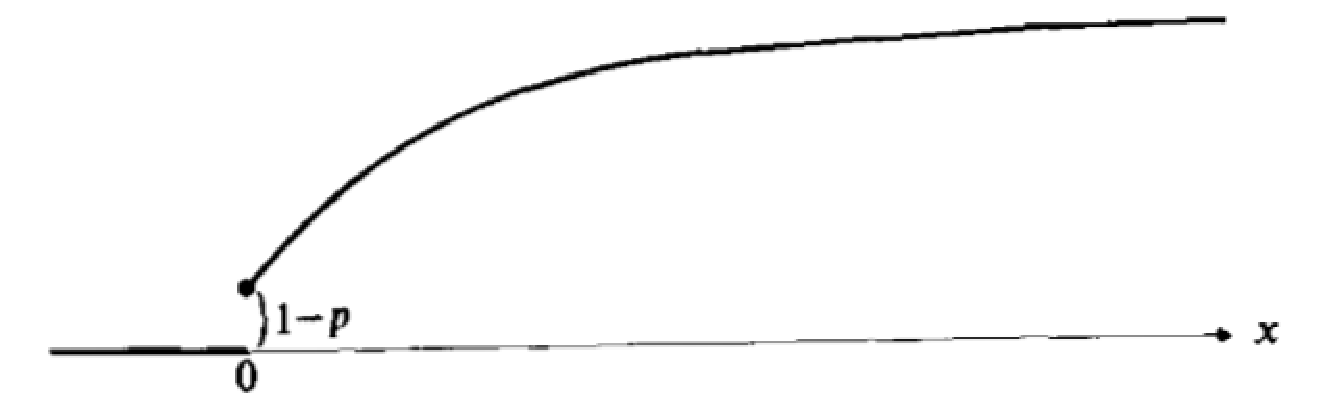
\includegraphics[scale = 0.5]{pictures/partially_continuous_and_discrete.eps}
\caption{Kumulativní distribuční funkce se skokem v $x = 0$ a spojitá pro $x > 0$}
\label{cross-road}
\end{figure}

Vedle toho existuje tzv. singulárně spojitá kumumlativní distribuční funkce, jejichž derivace je téměř ve všech bodech rovna nule. Tento typ kumulativní distribuční funkce je použit v následujícím tvrzení.
\begin{corollary}
Jakákoliv kumulativní distribuční funkce $F(x)$ může být vyjádřena ve formě
\begin{equation*}
F(x) = p_1 F^d(x) + p_2 F^{ac}(x) + p_3 F^{sc}(x)
\end{equation*}
kde $p_i \ge 0,~i = 1, 2, 3$, $\sum_{i=1}^3p_i = 1$, $F^d(\cdot)$ je nespojitá, $F^{ac}(\cdot)$ je absolutně spojitá a $F^{sc}(\cdot)$ je singulárně spojitá kumulativní distribuční funkce.
\end{corollary}

\begin{example}
Uvažujme $F_X(x) = (1-pe^{-\lambda x})I_{[0, \infty)}(x)$. Tuto kumulativní distribuční funkci lze rozepsat do tvaru
\begin{gather*}
F_X(x) = (1-p)F^d(x) + pF^{ac}(x) = (1-p)I_{[0,\infty)}(x) + p(1-e^{-\lambda x})I_{[0,\infty)}(x)\\
= (1 - pe^{-\lambda x})I_{[0, \infty]}(x)
\end{gather*}
\end{example}

Uvažujme $F(x) = (1-p)F^d(x) + pF^{ac}(x)$, kde $0 < p < 1$, $F^d(\cdot)$ je nespojitá a $F^{ac}(\cdot)$ je absolutně spojitá kumulativní distribuční funkce. Odpovídající pravděpodobnostní funkce je definováná jako $f(x) = (1-p)f^d(x) + p f^{ac}(x)$, kde $f^d(\cdot)$ je nespojitá pravděpodobnostní funkce odpovídající funkci $F^{d}(\cdot)$ a $f^{ac}(\cdot)$ je absolutně spojitá pravděpodobnostní funkce odpovídající funkci $F^{ac}(\cdot)$. Tato částečně nespojitá a částečně absolutně spojitá pravděpodobnostní funkce může být poměrně komplikovaná na interpretaci, a proto v takovýchto případech budeme spíše pracovat s kumulativní distribuční funkcí.

\section{Střední hodnoty a momenty}

\subsection{Střední hodnota}

\begin{definition}[Střední hodnota]
Uvažujme náhodnou veličinu $X$. Střední hodnota $X$, označovaná jako $E[X]$ popř. jako $\mu_x$, je definována následujím způsobem.
\begin{enumerate}
\item Jestliže je $X$ nespojité, pak
\begin{equation*}
E[X] = \sum x_j f_X(x_j)
\end{equation*}
pro body koncentrace $x_1, x_2, ..., x_j, ...$.
\item Jestliže je $X$ spojité, pak
\begin{equation*}
E[X] = \int_0^{\infty}x f_X(x)dx
\end{equation*}
\item Pro libovolné $X$ pak platí
\begin{equation*}
E[X] = \int_0^{\infty}[1 - F_X(x)]dx - \int_{-\infty}^0 F_X(x)dx
\end{equation*}
\end{enumerate}
V případě (1) $E[X]$ existuje, jestliže je daná řada absolutně konvergentní. V případě (2) $E[X]$ existuje, jestliže daný integrál existuje. Konečně, v případě (3) existuje $E[X]$, pokud jsou oba integrály konečné.
\end{definition}

Z definicí (1) a (2) je patrné, že na $E[X]$ je možné pohlížet jako na vážený průměr jednotlivých hodnot, kterých může náhodná veličina $X$ nabývat, přičemž vahami jsou příslušné pravděpodobnostni reprezentované pravděpodobnostní funkcí $f_X(x)$ popř. $f_X(x)dx$.

\begin{example}
Uvažujme hod hrací kostkou. Střední hodnota náhodné veličiny $X$, která představuje hodnotu hodu, je rovna
\begin{equation*}
E[X] = \sum_{i = 1}^6 i \frac{1}{6} = \frac{7}{2}
\end{equation*}
\end{example}

\begin{example}
Nechť je $X$ náhodná veličina s pravděpodobnostní funkcí $f_X(x) = \frac{1}{x^2}I_{[1,\infty)}(x)$. Pak
\begin{equation*}
E[X] = \int_1^{\infty} x \frac{1}{x^2}dx=\lim_{b \rightarrow \infty} \ln b = \infty
\end{equation*}
a proto $E[X]$ neexistuje.
\end{example}

\begin{example}
Nechť je $X$ náhodná veličina s kumulativní distribuční funkcí $F_X(x) = (1 - pe^{-\lambda x})I_{[0, \infty)}(x)$. Pak
\begin{equation*}
E[X] = \int_0^{\infty} [1 - F_X(x)]dx - \int_{-\infty}^0F_X(x)dx = \int_0^{\infty} p e^{-\lambda x}dx = \frac{p}{\lambda}
\end{equation*}
\end{example}

\subsection{Rozptyl}

\begin{definition}[Rozptyl]
Nechť je $X$ náhodná veličina se střední hodnotou $E[X]$. Roztyl této náhodné veličiny označovaný jako $D[X]$ resp. jako $\sigma_X^2$, je definován následujícím způsobem.
\begin{enumerate}
\item Jestliže je $X$ nespojité s body koncentrace $x_1, x_2, ..., x_n, ...$, pak
\begin{equation*}
D[X] = \sum_i(x_j - E[X])^2 f_X(x)
\end{equation*}
\item Jestliže je $X$ spojité, pak
\begin{equation*}
D[X] = \int_{-\infty}^{\infty}(x - E[X])^2 f_X(x)dx
\end{equation*}
\item Pro libovolnou náhodnou veličinu s kumulativní distribuční funkcí $F_X(x)$ platí
\begin{equation*}
D[X] = \int_0^{\infty} 2x[1 - F_X(x) + F_X(-x)]dx - E[X]^2
\end{equation*}
\end{enumerate}
Rozptyl je definován pouze tehdy, jestliže je řada v (1) absolutně konvergentní nebo jestliže integrály v (2) a (3) existují. Vzhledem k tomu, že $f_X(x) > 0$ pro všechna $x$, je rozptyl vždy kladný.
\end{definition}
Podobně jako střední hodnota i rozptyl je váženým průměrem. V obou případech jsou váhy shodné. V případě rozptylu se váží druhá mocnina odchylky náhodné veličiny od její střední hodnoty, kdežto v případě střední hodnoty se váží samotná hodnota náhodné veličiny.

\begin{definition}[Směrodatná odchylka]
Jestliže je $X$ náhodná veličina, pak je její směrodatná odchylka definována jako $\sigma_X = \sqrt{D[X]}$.
\end{definition}

Z výše uvedené definice je zřejmé, že směrodatná odchylka poskytuje stejnou informaci jako rozptyl. V řadě případů je však směrodatná odchylka preferována před rozptylem, protože je vyjádřena ve stejné měrné jednotce jako náhodná veličina.

\begin{example}
Uvažujme hod hrací kostkou. Rozptyl náhodné veličiny $X$ představující hodnotu hodu, je
\begin{equation*}
D[X] = \sum_{i = 1}^6 \big(i - \frac{7}{2} \big)^2 \frac{1}{6} = \frac{35}{12}
\end{equation*}
\end{example}

\begin{example}
Nechť je $X$ náhodná velična s pravděpodobnostní funkcí $f_X(x) = \lambda e^{-\lambda x}I_{[0, \infty)}(x)$. Střední hodnota náhodné veličiny $X$ je rovna $\frac{1}{\lambda}$ a její rozptyl je pak roven
\begin{equation*}
D[X] = \int_{-\infty}^{\infty} \big(x - \frac{1}{\lambda} \big)^2 \lambda e^{-\lambda x}dx = \frac{1}{\lambda^2}
\end{equation*}
\end{example}

\begin{example}
Nechť je $X$ náhodná veličina s kumulativní distribuční funkcí $F_X(x) = (1 - p e^{-\lambda x})I_{[0, \infty)}(x)$ a střední hodnotou $\frac{p}{\lambda}$. Rozptyl této náhodné veličiny je roven
\begin{equation*}
D[X] = \int_0^{\infty} 2x [1 - F(x) + F(-x)]dx - E[X]^2 = \int_0^{\infty}2x p e^{-\lambda x}dx - \big( \frac{p}{\lambda} \big)^2 = \frac{p(2 - p)}{\lambda^2}
\end{equation*}
\end{example}

\subsection{Střední hodnota funkce náhodné veličiny}

\begin{definition}[Střední hodnota funkce náhodné veličiny]
Nechť je $X$ náhodná veličina a $g(\cdot)$ je funkce s reálnou osou jako definičním oborem i oborem hodnot.
\begin{enumerate}
\item Jestliže je $X$ nespojité, pak
\begin{equation*}
E[g(X)] = \sum_jg(x_j)f_x(x_j)
\end{equation*}
\item Jestliže je $X$ spojité, pak
\begin{equation*}
E[g(X)] = \int_{-\infty}^{\infty} g(x)f_X(x)dx
\end{equation*}
\end{enumerate}
\end{definition}

\begin{theorem}
Střední hodnota funkce náhodné veličiny má následující vlastnosti.
\begin{enumerate}
\item $E[c] = c$ pro konstantu $c$
\item $E[c g(X)] = cE[g(X)]$ pro konstantu $c$
\item $E[c_1 g_1(X) + c_2 g_2(X)] = c_1 E[g_1(X)] + c_2 E[g_2(X)]$
\item $E[g_1(X)] \le E[g_2(X)]$ jestliže $g_1(x) \le g_2(x)$ pro všechna $x$
\end{enumerate}
\end{theorem}

\begin{theorem}[Výpočtový tvar rozptylu]
Jestliže je $X$ náhodná veličina, pak
\begin{equation*}
D[X] = E[X^2] - E[X]^2
\end{equation*}
za předpokladu, že $E[X]$ a $E[X^2]$ existují.
\end{theorem}

\begin{proof}
Z definice rozptylu a střední hodnoty funkce náhodné veličiny vyplývá $D[X] = E[X - E[X]^2]$. Tento vztah lze dále upravit do podoby
\begin{equation*}
E[X - E[X]^2] = E[X^2 - 2XE[X] + E[X]^2] = E[X^2] - 2E[X^2] + E[X^2] = E[X^2] - E[X]^2
\end{equation*}
\end{proof}

\subsection{Chebyshevova nerovnost}

\begin{theorem}
Nechť je $X$ náhodnou veličinou a $g(\cdot)$ nezápornou funkcí s reálnou osou jako definičním oborem. Pak
\begin{equation*}
P[g(X) \ge k] \le \frac{E[g(X)]}{k}~~~\textit{pro všechna}~k>0
\end{equation*}
\end{theorem}

\begin{proof}
Předpokládejme, že $X$ je spojitá náhodná veličina s pravděpodobnostní funkcí $f_X(\cdot)$. Pak
\begin{gather*}
E[g(X)] = \int_{-\infty}^{\infty} g(x)f_X(x)dx = \int_{x: g(x) \ge k} g(x) f_X(x)dx + \int_{x: g(x) < k}g(x)f_X(x)dx\\
\ge \int_{x: g(x) \ge k}g(x)f_X(x)dx \ge \int_{x: g(x) \ge k} k f_X(x)dx = k P[g(X) \ge k]
\end{gather*}
Důkaz završíme vydělením $k$. Analogický důkaz lze aplikovat také na nespojitou náhodnou veličinu.
\end{proof}

\begin{corollary}[Chebyshevova nerovnost]
Jestliže je $X$ náhodná veličina s konečným rozptylem, pak
\begin{equation*}
P[|X - E[X]| > r \sigma_X] = P[(X - E[X])^2 \ge r^2 \sigma_X^2] \le \frac{1}{r^2}~~~\textit{pro všechna}~r>0
\end{equation*}
\end{corollary}

\begin{proof}
Do věty (2.5) dosaďme $g(x) = (x - E[X]^2)$ a $k = r^2 \sigma_X^2$.
\end{proof}

Jedna z užitečných aplikací Chebyshevovy nerovnosti je následující. Pro náhodnou veličinu s konečným rozptylem platí
\begin{equation*}
P[|X - E[X]| < r \sigma_X] \ge 1 - \frac{1}{r^2}
\end{equation*}
což implikuje
\begin{equation*}
P[E[X] - r \sigma_X < X < E[X] + r \sigma_X] \ge 1 - \frac{1}{r^2}
\end{equation*}

\begin{example}
Pro $r = 2$ např. získáme $P[E[X] - 2 \sigma_X < X < E[X] + 2 \sigma_X] \ge \frac{3}{4}$. Libovolná náhodná veličina $X$ s konečným rozptylem se tak s pravděpodobností $\frac{3}{4}$ nachází do dvou směrodaných odchylek od své střední hodnoty. Toto zjištění platí pro všechny náhodné veličiny bez ohledu na jejich kumulativní distribuční funkci.
\end{example}

\subsection{Jensenova nerovnost}

\begin{definition}[Konvexní funkce]
Spojitá funkce $g(\cdot)$ s reálnou osou jako definičním oborem a oborem hodnot se nazývá konvexní, jestliže pro každé reálné $x_0$ existuje přímka, která prochází bodem $(x_0, g(x_0))$ a leží na nebo pod grafem funkce $g(\cdot)$.
\end{definition}

\begin{theorem}[Jensenova nerovnost]
Nechť je $X$ náhodná veličina se střední hodnotou $E[X]$ a nechť je $g(\cdot)$ konvexní funkcí. Pak $E[g(x)] \ge g(E[X])$.
\end{theorem}

\begin{proof}
Protože je $g(x)$ spojitá a konvexní funkce, pak existuje přímka $l(x) = a + bx$, která splňuje podmínky $l(x) = a + bx \ge g(x)$ a $l[E(X)] = g(E[X])$. Uvažovaná přímka $l(x)$ tak prochází bodem $(E[X], g(E[X]))$. Platí $E[l(X)] = E[(a + bX)] = a + bE[X] = l(E[X])$. Proto platí $g(E[X]) = l(E[X]) = E[l(X)] \le E[g(X)]$.
\end{proof}

Jensenova nerovnost mimojiné implikuje, že obecně nemusí platit $E[g(X)] = g(E[X])$. Dalším zajímavým důslekem  je, že pro konvexní funkci $g(x) = x^2$, platí $E[X^2] \ge E[X]^2$, což implikuje nezáporný rozptyl náhodné veličiny $X$.

\subsection{Momenty a momentová funkce}

\begin{definition}[Obecný moment]
Jestliže je $X$ náhodná veličina, je její $r$-tý obecný moment, označovaný jako $\mu_r'$, definován jako
\begin{equation*}
\mu_r' = E[X^r]
\end{equation*}
jestliže daná střední hodnota existuje.
\end{definition}

\begin{definition}[Centrální moment]
Jestliže je $X$ náhodná veličina, pak je $r$-tý centrální moment okolo $a$ definován jako $E[(X - a)^r]$. Jestliže $a = \mu_X$, pak centrální moment náhodné veličiny $X$ okolo $\mu_X$, označovaný jako $\mu_r$, je definován jako
\begin{equation*}
\mu_r = E[(X - \mu_X)^r]
\end{equation*}
\end{definition}

Z výše uvedeného je patrné, že $\mu_1 = E[(X - \mu_X)] = 0$ a $\mu_2 = E[(X - \mu_X)^2] = D[X]$. Dále platí, že liché centrální momenty náhodné veličiny $X$, jejíž pravděpodobnostní funkce je symetrická kolem $E[X]$, jsou rovny nule, pokud jsou tyto momenty definovány.

\begin{definition}[Vztah mezi obecným a centrálním momentem]
Platí, že z obecného momentu je možné odvodit centrální moment a naopak.
\begin{equation*}
\mu_k = \sum_{j = 0}^k \binom{k}{j}(-\mu_1')^j\mu_{k-1}'
\end{equation*}
\begin{equation*}
\mu_k = \sum_{j=0}^k \binom{k}{j} (\mu_1')^j\mu_{k-j}
\end{equation*}
\end{definition}

\begin{definition}[Kvantil]
$q$-tý kvantil náhodné veličiny $X$ je označován jako $\xi_q$ a definován jako nejmenší číslo $\xi$ splňující podmínku $F_X(\xi) \ge q$.
\end{definition}

\begin{definition}[Medián]
Medián náhodné veličiny $X$ označovaný jako $med_X$ nebo také $\xi_{0.50}$ je $0.5$-tým kvantilem.
\end{definition}

Jestliže je $X$ spojité, pak medián splňuje podmínku
\begin{equation*}
\int_{-\infty}^{med_x}f_X(x)dx = \frac{1}{2} = \int_{med_x}^{\infty}f_X(x)dx
\end{equation*}

\begin{definition}[Modus]
Další veličinou, kterou je možné použít k popisu ``centra'' náhodné veličiny $X$, je kromě střední hodnoty a mediánu tzv. modus. Modus je definován bod, pro který dosahuje $f_X(\cdot)$ maxima.
\end{definition}

Předpokládejme, že $f_1(x)$ a $f_2(x)$ jsou dvě pravděpodobnostní funkce se stejnou střední hodnotou $\mu$, které pro libovolné $a$ splňují podmínku
\begin{equation*}
\int_{\mu - a}^{\mu + a} [f_1(x) - f_2(x)]dx \ge 0
\end{equation*}
Takovéto pravděpodobnostní funkce jsou ilustrovány na následujícím obrázku.
\begin{figure}[htp]
\centering
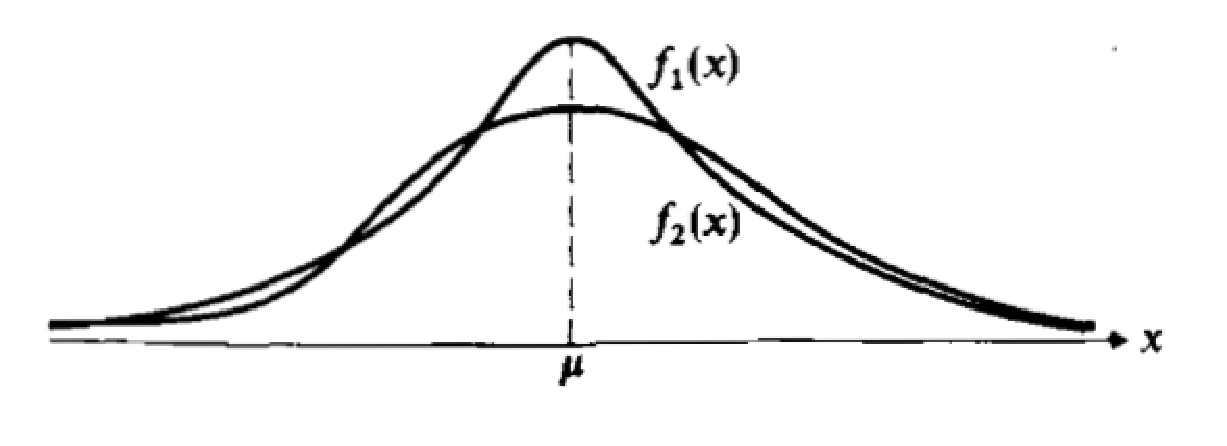
\includegraphics[scale = 0.5]{pictures/two_distributions.eps}
\caption{Pravděpodobnostní funkce $f_1(x)$ a $f_2(x)$ se shodnou střední hodnotou $\mu$}
\label{two_distributions}
\end{figure}
Lze dokázat, že rozptyl $\sigma_1^2$ pravděpodobnostní funkce $f_1(x)$ je menší než rozptyl $\sigma_2^2$ pravděpodobnostní funkce $f_2(x)$. Schéma důkazu je následující. Nechť $g(x) = f_1(x) - f_2(x)$, kde $f_1(x)$ a $f_2(x)$ splňují výše uvedenou podmínku. Protože z definice pravděpodobnostní funkce vyplývá $\int_{-\infty}^{\infty} g(x) dx = 0$, je v případě funkce $g(x)$ obsah ploch nad osou $x$ roven obsahu ploch od osou $x$. Dále je z podmínky pro funkce $f_1(x)$ a $f_2(x)$ patrné, že každý kladný element $g(x')dx'$ je vyvážen záporným elementem $g(x'')dx''$, kde $x''$ je dále od $\mu$ než $x'$. Jestliže tyto elementy násobíme $(x - \mu)^2$, jsou záporné elementy násobeny větším faktorem. Proto $\int_{-\infty}^{\infty}(x - \mu)^2 g(x) dx < 0$, pokud jsou $f_1(x)$ a $f_2(x)$ rozdílné. Z toho vyplývá $\sigma_1^2 < \sigma_2^2$.

Třetí centrální moment $\mu_3$ nazýváme mírou sešikmení. Pravděpodobnostní funkce, které jsou symetrické okolo své střední hodnoty, mají sešikmení $\mu_3 = 0$. Pravděpodobnostní funkce sešikmené do leva mají $\mu_3 < 0$. Pravděpodobnostní funkce sešikmené do prava pak mají $\mu_3 > 0$. Poněkud paradoxně nám však míra sešikmení neříká nic tvaru pravděpodobnostní funkce. Např. pravděpodobnostní funkce $f_4(x)$ na následujícím obrázku má $\mu_3 = 0$, avšak o symetrickou funkci se nejedná.
\figure[ht]\centering
\begin{pspicture}(14.0,3.0)
    \psline(0.0,0.5)(13.5,0.5)
      
    \pscurve[showpoints=false](0.0,0.6)(0.5,0.7)(1.5,2.0)(2.5,0.7)(3.0,0.6)
    \pscurve[showpoints=false](3.5,0.6)(4.0,0.7)(4.0,2.0)(6.0,0.7)(6.5,0.6)
    \pscurve[showpoints=false](7.0,0.6)(7.5,0.7)(9.0,2.0)(9.5,0.7)(10.0,0.6)
    \pscurve[showpoints=false](10.5,0.6)(11.0,0.7)(11.7,1.0)(12.0,2.0)(13.0,1.0)(13.5,0.6)

    \rput(1.5,2.3){\psframebox*{\tiny{$f_1(x): \mu = 0$}}}
    \rput(1.5,0.2){\psframebox*{\tiny{(a)}}}
    \rput(4.0,2.3){\psframebox*{\tiny{$f_2(x): \mu < 0$}}}
    \rput(5.0,0.2){\psframebox*{\tiny{(b)}}}
    \rput(9.0,2.3){\psframebox*{\tiny{$f_3(x): \mu > 0$}}}
    \rput(8.5,0.2){\psframebox*{\tiny{(c)}}}
    \rput(12.0,2.3){\psframebox*{\tiny{$f_4(x): \mu = 0$}}}
    \rput(12.0,0.2){\psframebox*{\tiny{(d)}}}

  \end{pspicture}
  \caption{Pravděpodobnostní funkce s rozdílnou mírou sešikmení}
\endfigure
Alternativním ukazatelem sešikmení je
\begin{equation*}
s = \frac{\textit{průměr - medián}}{\textit{směrodatná odchylka}}
\end{equation*}
Lze dokázat, že $-1 \le s \le 1$.

Čtvrtý centrální moment se používá jako ukazatel zakřivení, která vyjadřuje míru ``plochosti'' pravděpodobnostní funkce v okolí jejího středu. Pozitivní hodnota $\frac{\mu_4}{\sigma^4}-3$ indikuje, že daná pravděpodobnostní funkce je v okolí svého středu více ``špičatá'' než pravděpodobnostní funkce normálního rozdělení. Naopak, negativní hodnota $\frac{\mu_4}{\sigma^4}-3$ indikuje, že daná pravděpodobnostní funkce je v okolí svého středu více ``plochá'' než pravděpodobnostní funkce normálního rozdělení. Podobně jako v případě sešikmení, ani v případě zakřivení není tento ukazatel vždy směrodatný pro tvar pravděpodobnostní funkce.

Ačkoliv několik momentů může postkytnout pouze omezenou informaci o pravděpodobnostní funkci, soubor všech momentů definuje pravděpodobnostní funkci jednoznačně.

\begin{figure}[htp]
\centering
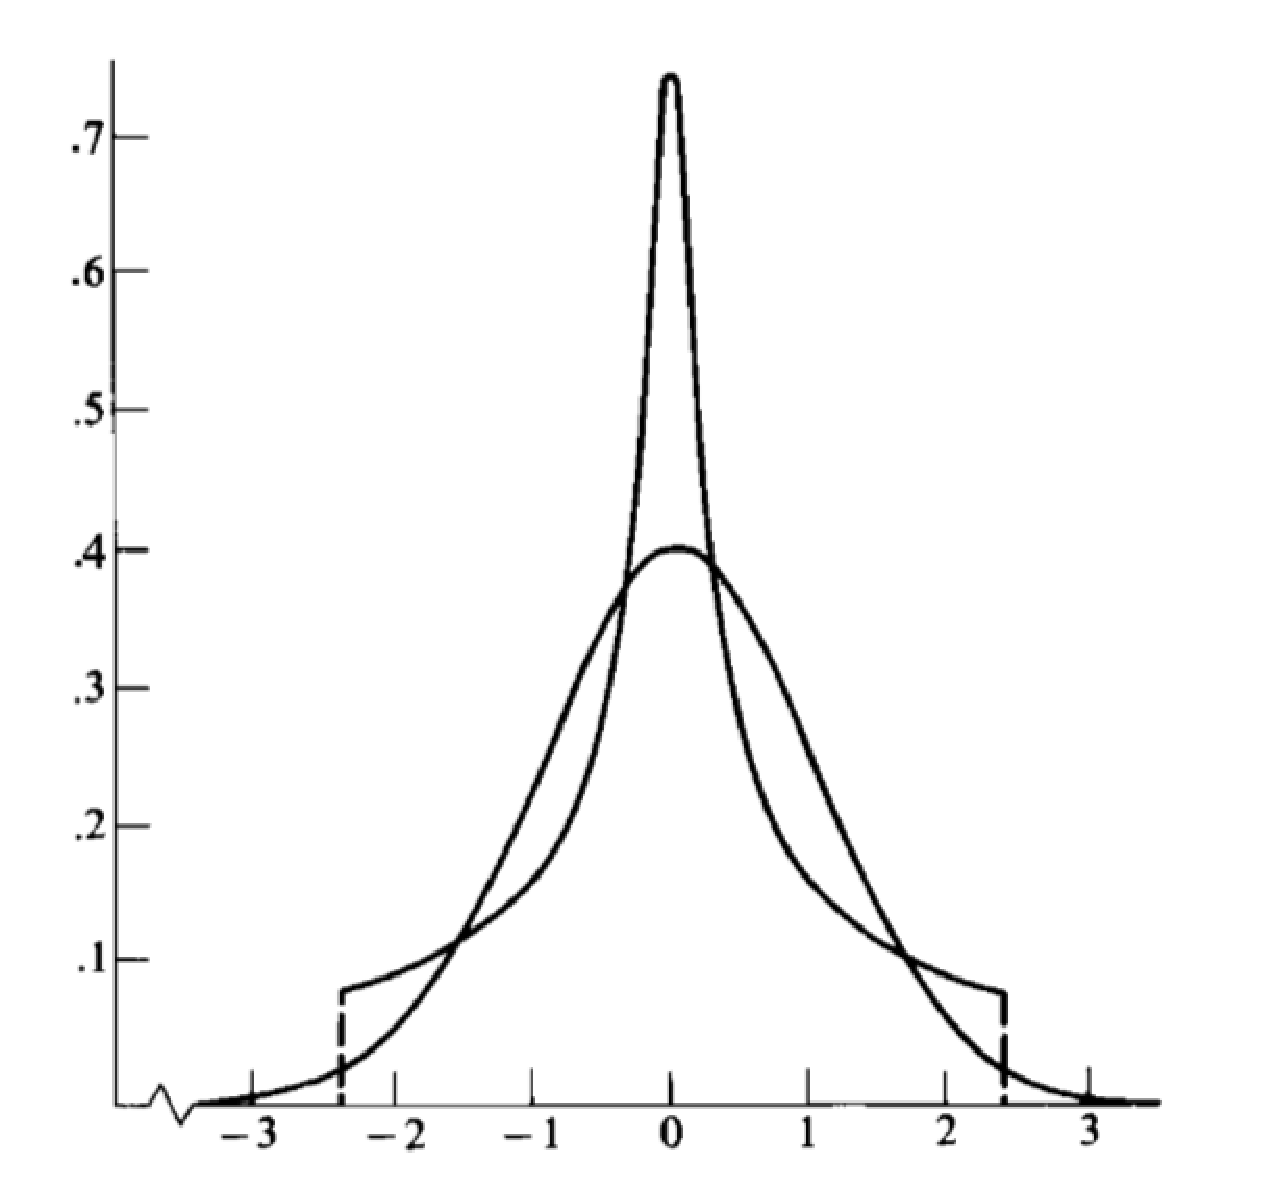
\includegraphics[scale = 0.3]{pictures/first_four_moments.eps}
\caption{Dvě pravděpodobnostní funkce se shodnými prvními čtyřmi momenty}
\label{first_four_moments}
\end{figure}

V aplikované statistice hrají klíčovou roli především první dva momenty, třetí a čtvrtý moment se používají vyjímečně a vyšší momenty pak téměr vůbec.

\begin{definition}[Faktoriální moment]
Jestliže je $X$ náhodnou veličinou, pak $r$-tý faktoriální moment $X$ je definován jako
\begin{equation*}
E[X(X-1) \cdots (X - r + 1)]
\end{equation*}
\end{definition}
Pro některé, zpravidla nespojité, náhodné veličiny je snazší vypočíst faktoriální moment než obecný popř. centrální moment. Nicméně platí, že z faktoriálního momentu lze odvodit obecný popř. centrální moment a naopak.

\begin{definition}[Momentová funkce]
Nechť je $X$ náhodná veličina s pravděpodobnostní funkcí $f_X(\cdot)$. Očekávaná hodnota $e^{tX}$ je definuje tzv. momentovou funkci, jestliže tato očekávaná hodnota existuje pro každé $t$ v intervalu $-h < t < h$ pro $h > 0$. Momentová funkce má tvar
\begin{equation*}
m(t) = E[e^{tx}] = \int_{-\infty}^{\infty} e^{tx}f_X(x)dx
\end{equation*}
je-li $X$ spojité a
\begin{equation*}
m(t) = E[e^{tx}] = \sum_x e^{tx}f_X(x)
\end{equation*}
je-li $X$ nespojité.
\end{definition}

Existuje-li momentová funkce, pak je spojitě diferenciovatelná v okolí počátku. Jestliže momentovou funkci $r$ krát derivujeme vzhledem k $t$, pak získáme
\begin{equation*}
\frac{d^r}{dt^r}m(t) = \int_{-\infty}^{\infty}x^r e^{xt}f_X(x)dx
\end{equation*}
a jestliže $r \rightarrow 0$, pak
\begin{equation*}
\frac{d^r}{dt^r}m(0) = E[X^r] = \mu_r'
\end{equation*}
Momenty pravděpodobnostní funkce tak lze získat z momentové funkce její derivací dle $t$.

Jestliže v momentové funkci nahradíme $e^{tx}$ Taylorovým rozvojem, pak získáme
\begin{equation*}
m(t) = E\big[1 + tX + \frac{1}{2!}(tX)^2 + \frac{1}{3!}(tX)^3 + \cdots \big] = 1 + \mu_1't + \frac{1}{2!}\mu_2't^2 + \cdots = \sum_{t = 0}^{\infty}\frac{1}{i!}\mu_t't^i
\end{equation*}
Z výše uvedené rovnice je patrné, že $\mu_r'$ lze získat z Taylorova rozvoje $m(t)$ jako koeficient prvku $\frac{t^r}{r!}$.

\begin{example}
Nechť je $X$ náhodná veličina s pravděpodobnostní funkcí $f_X(x) = \lambda e^{-\lambda x}I_{[0, \infty)}(x)$. Pak
\begin{equation*}
m(t) = E[e^{tX}] = \int_0^{\infty} e^{tx} \lambda e^{-\lambda x} dx = \frac{\lambda}{\lambda - t}~~~\textit{pro}~t < \lambda
\end{equation*}
a proto
\begin{equation*}
m'(t) = \frac{\lambda}{(\lambda - t)^2}~~~\textit{což implikuje}~~~m'(0) = E[X] = \frac{1}{\lambda}
\end{equation*}
\begin{equation*}
m''(t) = \frac{2 \lambda}{(\lambda - t)^3}~~~\textit{což implikuje}~~~m''(0) = E[X^2] = \frac{2}{\lambda^2}
\end{equation*}
\end{example}

\begin{example}
Uvažujme náhodnou veličinu $X$ s pravděpodobnostní funkcí $f_X(x) = x^{-2}I_{[1, \infty)}(x)$. Kdyby momentová funkce této náhodné veličiny existovala, pak by byla dána rovnicí $\int_1^{\infty}X^{-2}e^{tx}dx$. Lze však dokázat, že takovýto integrál neexistuje pro žádné $t > 0$, a proto také neexistuje tato momentová funkce.
\end{example}

\begin{definition}[Faktoriální momentová funkce]
Nechť je $X$ náhodná veličina. Faktoriální momentová funkce je definována jako $E[t^x]$, jestliže tato střední hodnota existuje.
\end{definition}

Faktoriální momentovou funkci lze použít pro generování faktoriálních momentů stejným způsobem jakým lze odvodit obecný moment z momentové funkce. Jediným rozdílem je, že $t \rightarrow 1$ namísto $t \rightarrow 0$. Tento postup někdy zjednodušuje nalezení momentu v případě nespojité pravděpodobnostní funkce.

\begin{example}
Nechť je $X$ náhodná veličina s nespojitou pravděpodobostní funkcí
\begin{equation*}
f_X(x) = \frac{e^{-\lambda}\lambda^x}{x!}
\end{equation*}
Pak
\begin{equation*}
E[t^X] = \sum_{x = 0}^{\infty} \frac{t^x e^{-\lambda} \lambda^x}{x!} = e^{-\lambda} e^{\lambda t} = e^{\lambda(t - 1)}
\end{equation*}
\begin{equation*}
\frac{d}{dt}E[t^X] = \frac{d}{dt} e^{\lambda(t-1)}=\lambda e^{\lambda (t - 1)}~~~\textit{a proto}~~~\frac{d}{dt}E[t^X] \Big|_{t = 1} = \lambda
\end{equation*}
\end{example}

Momentovou funkci lze, jak její název napovídá, použít k výpočtu momentů. Vedle toho ji však lze také použít k určení pravděpodobnostní funkce.

\begin{theorem}
Nechť jsou $X$ a $Y$ dvě náhodné veličiny s pravděpodobnostními funkcemi $f_X(\cdot)$ a $f_Y(\cdot)$. Předpokládejme, že jejich momentové funkce $m_X(t)$ a $m_Y(t)$ existují a jsou shodné pro všechna $t$ z intervalu $-h < t < h$ pro $h > 0$. Potom jsou shodné také pravděpodobnostní funkce $f_X(\cdot)$ a $f_Y(\cdot)$.
\end{theorem}

\chapter{Vybraná pravděpodobnostní rozdělení}

Nejčastěji používané pravděpodobnostní funkce mají přiřazeno jméno. Říkáme tak např., že daná náhodná veličina sleduje normální pravděpodobnostní rozdělení. Stejně jako náhodné veličiny také pravděpodobnostní rozdělení dělíme na spojitá a nespojitá. Následující kapitola je stručným přehledem v praxi nejběžněji používaných pravděpodobnostních rozdělení.

\section{Nespojité pravděpodobnostní rozdělení}

\subsection{Nespojité uniformní rozdělení}

\begin{definition}[Nespojité uniformní rozdělení]
Jestliže má náhodná veličina $X$ pravděpodobnostní funkci
\begin{gather*}
f(x) =
\begin{cases}
\frac{1}{N}~~~\textit{pro}~x = 1,2, ..., N\\
0~~~\textit{v ostatních případech}
\end{cases}\\
=\frac{1}{N}I_{\{1, 2, ..., N\}}(x)
\end{gather*}
kde $N$ je přirozené číslo, říkáme, že tato náhodná veličina sleduje nespojité uniformní rozdělení.
\end{definition}

\begin{figure}[htp]
\centering
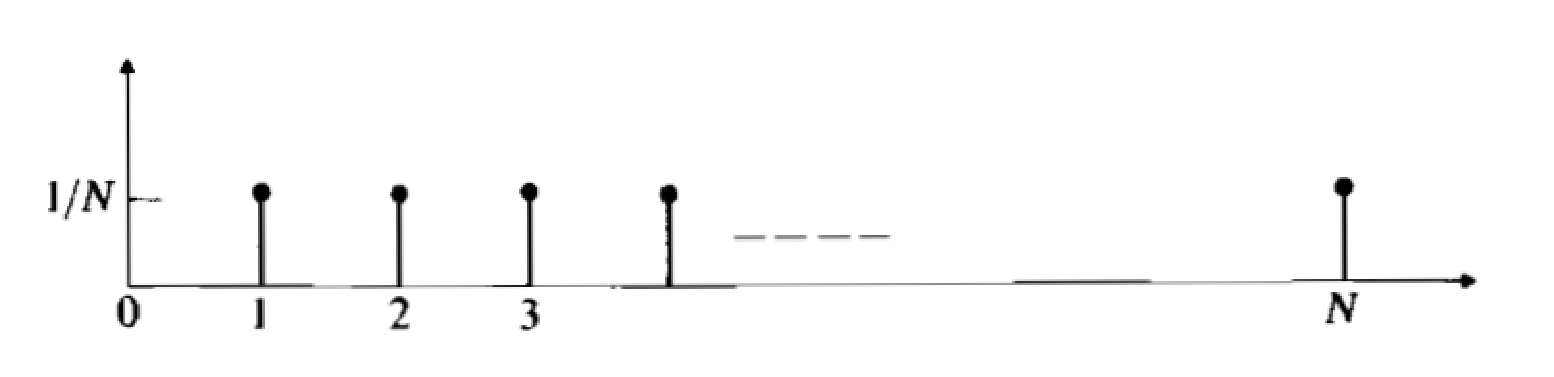
\includegraphics[scale = 0.5]{pictures/discrete_uniform_distribution.eps}
\caption{Pravděpodobnostní funkce nespojitého uniformního rozdělení}
\label{discrete_uniform_distribution}
\end{figure}  

\begin{theorem}
Jestliže náhodná veličina $X$ sleduje nespojité uniformní rozdělení, pak
\begin{gather*}
E[X] = \frac{N+1}{2}\\
D[X] = \frac{N^2 - 1}{12}\\
m(t) = E[e^{tX}] = \sum_{j = 1}^N e^{jt}\frac{1}{N}
\end{gather*}
\end{theorem}

\begin{proof}
\begin{gather*}
E[X] = \sum_{j = 1}^N j \frac{1}{N} = \frac{N+1}{2}\\
D[X] = E[X^2] - E[X]^2 = \sum_{j=1}^N j^2 \frac{1}{N} - \Big( \frac{N+1}{2} \Big)^2\\
= \frac{N(N+1)(2N+1)}{6N} - \frac{(N+1)^2}{4} = \frac{(N+1)(N-1)}{12}\\
E[e^{tX}] = \sum_{j = 1}^N e^{jt} \frac{1}{N}
\end{gather*}
\end{proof}

Někdy je nespojité diskrétní rozdělení definována jako
\begin{equation*}
f(x) = \frac{1}{N+1}I_{\{0,1,...,N\}}(x)
\end{equation*}
V těchto případech je třeba výše uvedené rovnice upravit.

\subsection{Bernoulliho a binomické rozdělení}

\subsubsection{Bernoulliho rozdělení}

\begin{definition}[Bernoulliho rozdělení]
Říkáme, že náhodná veličina $X$ sleduje Bernoulliho rozdělení, jestliže má její pravděpodobnostní rozdělení tvar
\begin{equation*}
f(x) =
\begin{cases}
p^x(1-p)^{1-x}~~~\text{pro}~x = 0, 1\\
0~~~\textit{v ostatních případech}
\end{cases}\\
= p^x(1-p)^{1-x}I_{\{0,1\}}(x)
\end{equation*}
kde $0 \le p \le 1$. Parameter $1-p$ se velmi často označuje jako $q$.
\end{definition}

\begin{figure}[htp]
\centering
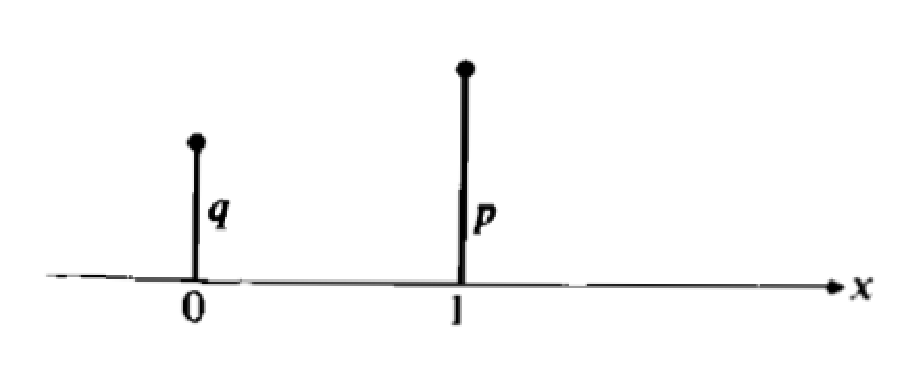
\includegraphics[scale = 0.5]{pictures/bernoulli_distribution.eps}
\caption{Pravděpodobnostní funkce Bernoulliho rozdělení}
\label{bernoulli_distribution}
\end{figure}  

\begin{theorem}
Jestliže náhodná veličina $X$ sleduje Bernoulliho rozdělení, pak
\begin{gather*}
E[X] = p\\
D[X] = pq\\
m(t) = pe^t + q\\
\end{gather*}
\end{theorem}

\begin{proof}
\begin{gather*}
E[X] = 0 \cdot q + 1 \cdot p = p\\
D[X] = E[X^2] - E[X]^2 = 0^2 \cdot q + 1^2 \cdot p - p^2 = pq\\
m(t) = E[e^{tX}] = e^{0 \cdot t} p^0 q^1 + e^{1 \cdot t} p^1 q^0 = q + e^t p
\end{gather*}
\end{proof}

\begin{example}
Uvažujme hod hrací kostkou. Úspěch definujme jako situaci, kdy padne číslo šest a neúspěch, jestliže padne číslo jedna až pět. Odpovídající náhodná veličina má povahu Bernoulliho rozdělení s pravděpodobností úspěchu $p = \frac{1}{6}$.
\end{example}

\subsubsection{Binomické rozdělení}

\begin{definition}[Binomické rozdělení]
Náhodná veličina $X$ sleduje binomické rozdělení, jestliže její pravděpodobnostní funkce je
\begin{equation*}
f(x) = 
\begin{cases}
\binom{n}{x} p^x q^{n-x}~~~\textit{pro}~x=0,1,...,n\\
0~~~\textit{v ostatních případech}
\end{cases}\\
=\binom{n}{x}p^xq^{n-x}I_{\{0,1,...,n\}}(x)
\end{equation*}
kde $0 \le p \le 1$, $n$ je přirozené číslo a $q = 1 - p$.
\end{definition}

\begin{figure}[htp]
\centering
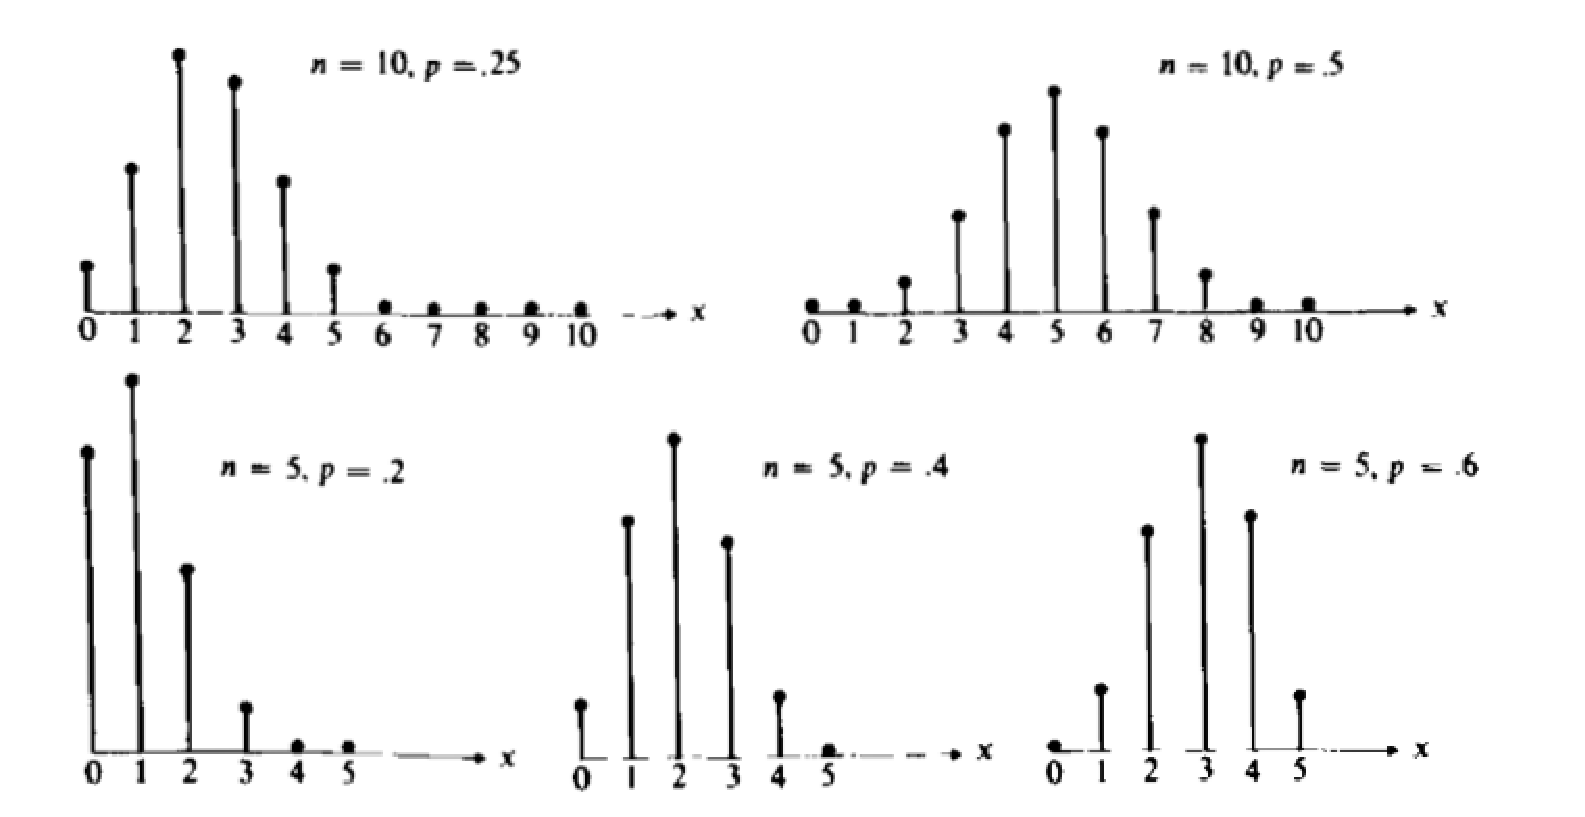
\includegraphics[scale = 0.5]{pictures/binomial_distribution.eps}
\caption{Pravděpodobnostní funkce binomického rozdělení}
\label{binomial_distribution}
\end{figure} 

\begin{theorem}
Jestliže náhodná velčina $X$ sleduje binomické rozdělení, pak
\begin{gather*}
E[X] = np\\
D[X] = npq\\
m(t) = (q + pe^t)^n
\end{gather*}
\end{theorem}

\begin{proof}
\begin{gather*}
m(t) = E[e^{tX}] = \sum_{x=0}^ne^{tx}\binom{n}{x}p^x q^{n-x}=\sum_{x=0}^n \binom{n}{x}(pe^t)^xq^{n-x} = (pe^t + q)^n\\
m'(t) = npe^t(pe^t + q)^{n-1}\\
m''(t) = n(n-1)(pe^t)^2(pe^t + q)^{n-2} + npe^t(pe^t + q)^{n-1}
\end{gather*}
a proto
\begin{gather*}
E[X] =  m'(0) = np\\
D[X] = E[X^2] - E[X]^2 = m''(0) - (np)^2 = n(n-1)p^2 + np - (np)^2 = np(1-p)
\end{gather*}
\end{proof}
Je-li $n=1$ zredukuje se binomické na Bernoulliho rozdělení.
\begin{example}
Uvažujme hod pěti hracími kostkami. Jaká je pravděpodobnost, že číslo šest padne právě dvakrát?

Jedním z možných řešení je situace, kdy v prvních třech hodech padlo číslo jedna až pět a číslo šest padlo v posledních dvou hodech. Pravděpodobnost této kombinace je $\big(\frac{5}{6}\big)^3\big(\frac{1}{6}\big)^2$. Vzhledem k tomu, že však nezáleží na pořadí hodů, existuje $\binom{5}{2}$ takovýchto řešení. Výsledná pravděpodobnost je tak rovna
\begin{equation*}
\binom{5}{2}\Big(\frac{5}{6}\Big)^3\Big(\frac{1}{6}\Big)^2 = 0.1608
\end{equation*} 
\end{example}

Jak vyplývá z následující věty, pravděpodobnostní funkce binomického rozdělení nejprve monotónně roste a následně monotónně klesá.
\begin{theorem}
Nechť náhodná veličina $X$ sleduje binomické rozdělení. Pak
\begin{enumerate}
\item $f(x-1) < f(x)$ jestliže $x < (n + 1)p$,
\item $f(x-1) > f(x)$ jestliže $x > (n + 1)p$ a
\item $f(x-1) = f(x)$ jestliže $x = (n + 1)p$ a $(n + 1)p$ je celé číslo pro $x = 1, 2, ...,n$.
\end{enumerate}
\end{theorem}

\begin{proof}
\begin{equation*}
\frac{f(x)}{f(x-1)} = \frac{n - x + 1}{x} \frac{p}{q} = 1 + \frac{(n + 1)p - x}{xq}
\end{equation*}
Výše uvedené je
\begin{enumerate}
\item větší než 1, jestliže $x < (n + 1)x$,
\item menší než 1, jestliže $x > (n + 1)x$ a
\item rovno 1, jestliže $x = (n + 1)x$.
\end{enumerate}
\end{proof}

\subsection{Hypergeometrické rozdělení}

\begin{definition}[Hypergeometrické rozdělení]
Jestliže náhodná veličina $X$ sleduje hypergeometrické rozdělení, pak je její pravděpodobnostní funkce definována jako
\begin{gather*}
f(x) =
\begin{cases}
\frac{\binom{K}{x}\binom{M-K}{n-x}}{\binom{M}{n}}~~~\textit{pro}~x = 0,1,...,n\\
0~~~\textit{v ostatních případech}
\end{cases}\\
= \frac{\binom{K}{x}\binom{M-K}{n-x}}{\binom{M}{n}}I_{\{0,1,...,n\}}(x)
\end{gather*}
kde $M > 0$, $0 \le K \le M$, $0 < n \le M$. 
\end{definition}

\begin{figure}[htp]
\centering
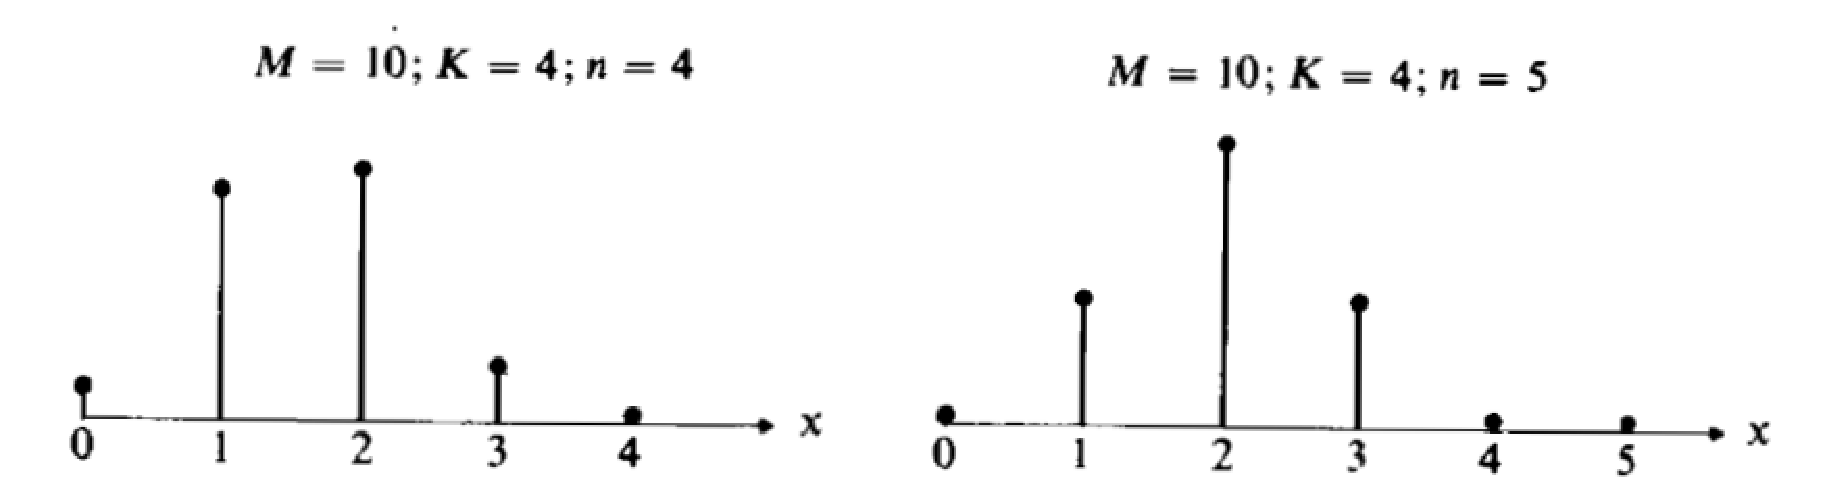
\includegraphics[scale = 0.5]{pictures/hypergeometric_distribution.eps}
\caption{Pravděpodobnostní funkce hypergeometrického rozdělení}
\label{hypergeometric_distribution}
\end{figure}

\begin{theorem}
Jestliže náhodná veličina $X$ sleduje hypergeometrické rozdělení, pak
\begin{gather*}
E[X] = n \frac{K}{M}\\
D[X] = n \frac{K}{M} \frac{M-K}{M}\frac{M-n}{M-1}
\end{gather*}
\end{theorem}

\begin{proof}
\begin{gather*}
E[X] = \sum_{x=0}^n x \frac{\binom{K}{x}\binom{M - K}{n-x}}{\binom{M}{n}} = n \frac{K}{M}\sum_{x=1}^n \frac{\binom{K-1}{x-1}\binom{M-K}{n-x}}{\binom{M-1}{n-1}}\\
= n \frac{K}{M} \sum_{y=0}^{n-1} \frac{\binom{K-1}{y}\binom{M-1-K+1}{n-1-y}}{\binom{M-1}{n-1}}=n \frac{K}{M}
\end{gather*}
s využitím vztahů $\binom{a}{b} = \frac{a}{b}\binom{a-1}{b-1}$ a $\sum_{i=0}^m \binom{a}{i}\binom{b}{m-i} = \binom{a + b}{m}$. Dále platí
\begin{gather*}
E[X(X-1)] = \sum_{x = 0}^n x(x-1)\frac{\binom{K}{x} \binom{M-K}{n-x}}{\binom{M}{n}} = n(n-1)\frac{K(K-1)}{M(M-1)}\sum_{x=2}^n \frac{\binom{K-2}{x-2}\binom{M-K}{n-x}}{\frac{M-2}{n-2}}\\
= n(n-1)\frac{K(K-1)}{M(M-1)}\sum_{y=0}^{n-2} \frac{\binom{K-2}{y}\binom{M-2-K+2}{n-2-y}}{\binom{M-2}{n-2}} = n (n-1) \frac{K(K-1)}{M(M-1)}
\end{gather*}
A proto
\begin{gather*}
D[X] = E[X^2] - E[X]^2 = E[X(X-1)] + E[X] - E[X]^2\\
= n(n-1)\frac{K(K-1)}{M(M-1)} + n \frac{K}{M}-n^2 \frac{K^2}{M^2} = n \frac{K}{M}\Big((n-1)\frac{K-1}{M-1} + 1 - \frac{nK}{M} \Big)\\
= \frac{nK}{M}\Big(\frac{(M-K)(M-n)}{M(M-1)} \Big)
\end{gather*}
\end{proof}

Jestliže dosadíme $\frac{K}{M} = p$, pak se střední hodnota hypergeometrického rozdělení shoduje se střední hodnotou binomického rozdělení a rozptyl hypergeometrického rozdělení je $\frac{M-n}{M-1}$ krát rozptyl binomického rozdělení.

\begin{example}
Nechť $X$ označuje počet vadných výrobků ve vzorku velikosti $n$, který byl získán výběrem bez vracení z populace $M$ výrobků, z nichž celkem $K$ bylo vadných. Takto definovaná náhodná veličina sleduje hypergeometrické rozdělení.
\end{example}

\subsection{Poissonovo rozdělení}

\begin{definition}[Poissonovo rozdělení]
Náhodná veličina $X$ sleduje Poissonovo rozdělení, jestliže její pravděpodobnostní funkce je definována jako
\begin{gather*}
f(x) =
\begin{cases}
\frac{e^{-\lambda}\lambda^x}{x!}~~~\textit{pro}~x = 0,1,2, ...\\
0 ~~~\textit{v ostatních případech}
\end{cases}\\
= \frac{e^{-\lambda}\lambda^x}{x!}I_{\{0,1,2, ...\}}(x)
\end{gather*}
kde $\lambda > 0$.
\end{definition}

\begin{figure}[htp]
\centering
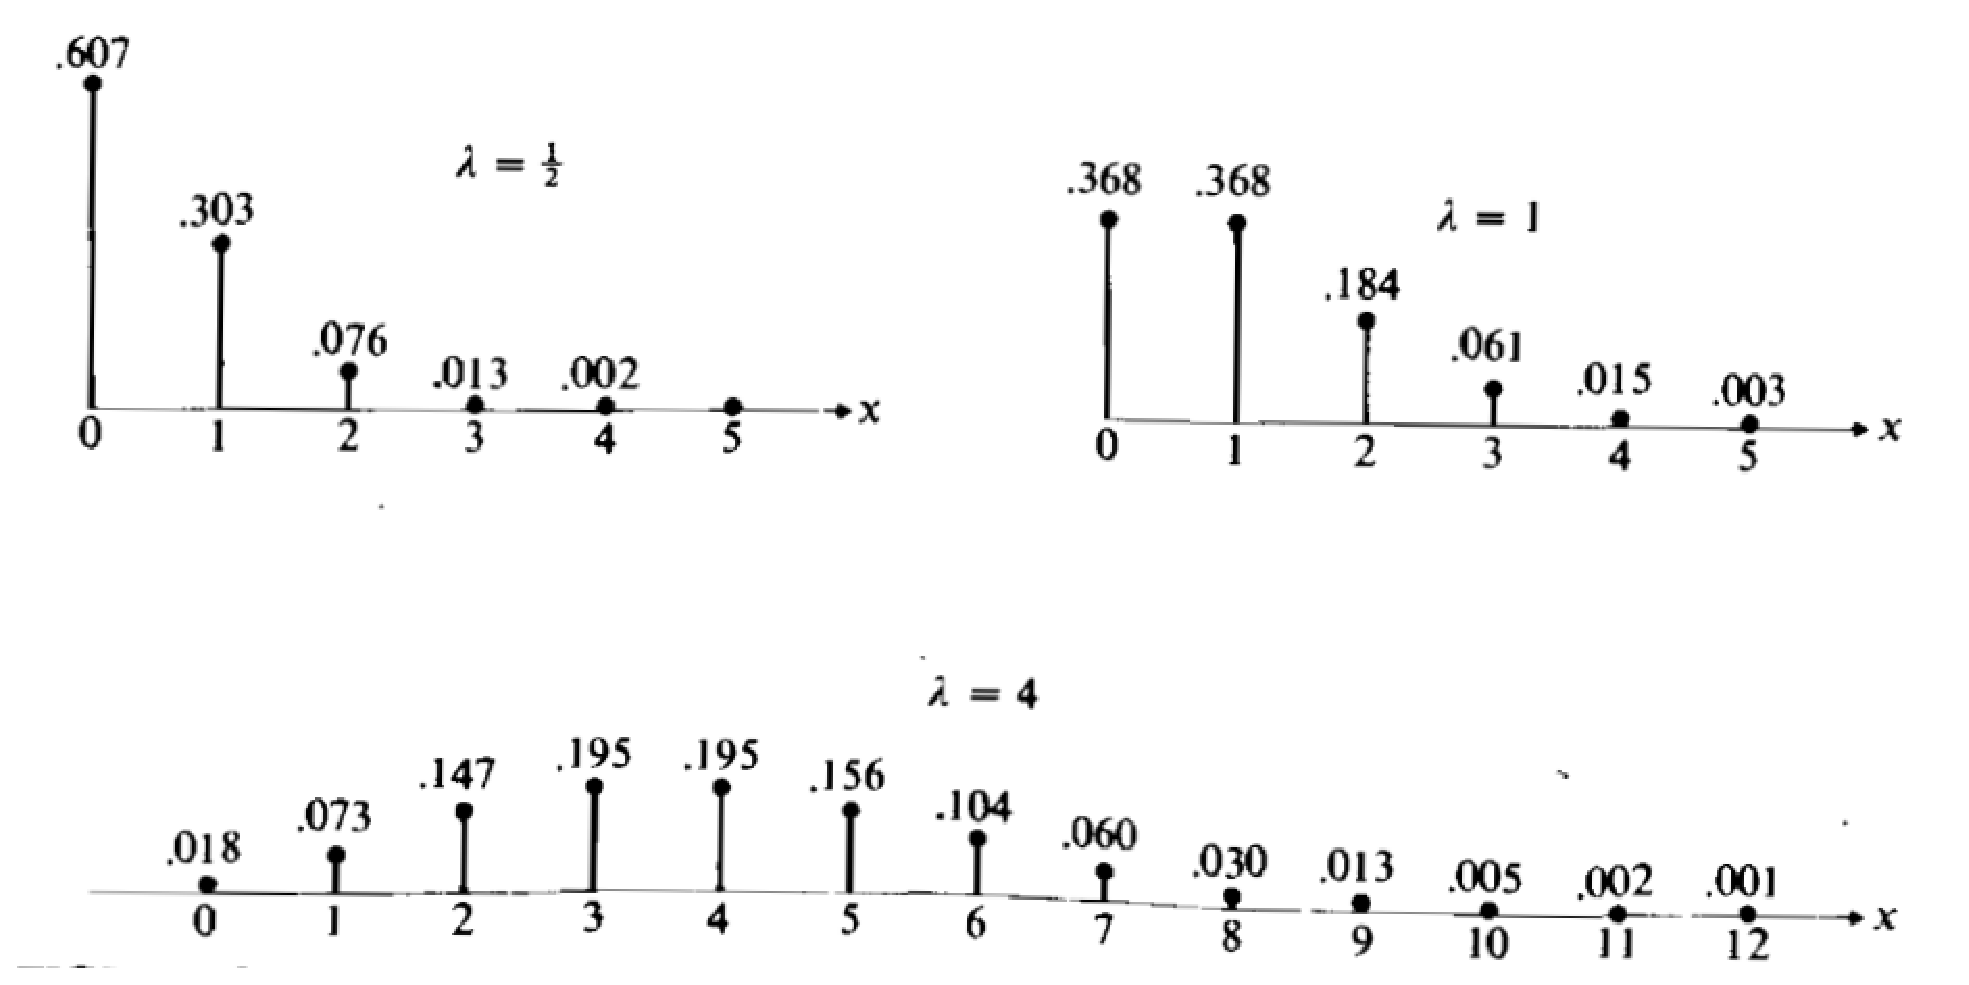
\includegraphics[scale = 0.35]{pictures/poisson_distribution.eps}
\caption{Pravděpodobnostní funkce Poissonova rozdělení}
\label{poisson_distribution}
\end{figure}

\begin{theorem}
Nechť náhodná veličina $X$ sleduje Poissonovo rozdělení. Pak
\begin{gather*}
E[X] = \lambda\\
D[X] = \lambda\\
m(t) = e^{\lambda (e^t - 1)}
\end{gather*}
\end{theorem}

\begin{proof}
\begin{gather*}
m(t) = E[e^{tX}] = \sum_{x = 0}^{\infty} \frac{e^{tx} e^{-\lambda} \lambda^x}{x!} = e^{-\lambda} \sum_{x = 0}^{\infty} \frac{(\lambda e^t)^x}{x!} = e^{-\lambda}e^{\lambda e^t}\\
m'(t) = \lambda e^{-\lambda} e^t e^{\lambda e^t}\\
m''(t) = \lambda e^{-\lambda} e^t e^{-\lambda e^t}(\lambda e^t + 1)
\end{gather*}
Proto
\begin{gather*}
E[X] = m'(0) = \lambda\\
D[X] = E[X^2] - E[X]^2 = m''(0) - \lambda^2 = \lambda(\lambda + 1) - \lambda^2 = \lambda
\end{gather*}
\end{proof}

Poissonovo rozdělení je vhodné pro modelování počtu realizací vzájemně nezávislých náhodných událostí vztažených k času, objemu, délce nebo ploše. Příkladem může být počet radioaktivních částic emitovaných za jednotku času, počet mikroorganismů v daném objemu roztoku, množství poškození DNA na jeden nanometer nebo počet kazů na metr čtvereční vyrobené látky. V některých situacích, které jsou na první pohled analogií výše uvedených příkladů, je použití Poissonova rozdělení nevhodné. Příkladem může být počet škůdců na hektar zemědělské půdy, kde není splněn předpoklad vzájemné nezávislosti\footnote{Pokud je škůdce nalezen na určitém místě, je pravděpodobné, že se bude nacházet také v jeho okolí. Škůdci se tak na poli nenachází náhodně, ale vytváří ohniska nákazy.}. Klíčové je Poissonovo rozdělení pro pojistnou matematiku neživotního pojištění, kde slouží k modelování počtu pojistných událostí.

Uvažujme $v > 0$, které vyjadřuje pravděpodobnost realizace náhodné události a které splňuje následující tři podmínky.
\begin{enumerate}
\item Pravděpodobnost právě jedné realizace v krátkém časovém intervalu délky $h$ je přibližně rovno $vh$, nebo-li $P[\textit{jedna realizace za časový interval } h] = vh + o(h)$.
\item Pravděpodobnost dvou a více realizací v časovém intervalu délky $h$ je zanedbatelné v porovnání s pravděpodobnostní jedné realizace v témže časovém intervalu, nebo-li $P[\textit{dvě a více realizací za časový interval } h] = o(h)$.
\item Počty realizací v nepřekrývajících se časových intervalech jsou vzájemně nezávislé. 
\end{enumerate}
$o(h)$ označuje funkci nižšího řádu než $h$, která splňuje podmínku
\begin{equation*}
\lim_{h \rightarrow 0} \frac{o(h)}{h} = 0
\end{equation*}
Hodnotu $v$ lze interpretovat jako střední míru realizace za časovou jednotku.

\begin{theorem}
Jestliže jsou výše uvedené tři podmínky splněny, pak počet realizací v čase $t$ má Poissonovo rozdělení s parametrem $\lambda = v t$. Nebo-li jestliže náhodná veličina $Z(t)$ označuje počet realizací v časovém intervalu délky $t$, pak $P[Z(t) = z] = e^{-vt}\frac{(vt)^z}{z!}$ pro $z = 0, 1, 2, ...$.
\end{theorem}

\begin{proof}[První způsob]
Uvažujme časový interval $(0, t]$ o délce $t$ a časový interval $(t, t + h]$ o délce $h$. Definujme
\begin{equation*}
P_n(s) = P[Z(s) = n] = P[\textit{právě } n \textit{ realizací v časovém intervalu délky } s]
\end{equation*}
Pak, na základě podmínky (3) o vzájemné nezávislosti, platí
\begin{gather*}
P_0(t + h) = P\big[0 \textit{ realizací v časovém intervalu } (0, t + h]\big]\\
= P\big[0 \textit{ realizací v } (0, t] \textit{ a } 0 \textit{ realizací v } (t, t + h] \big]\\
= P\big[0 \textit{ realizací v } (0, t] \big]P \big[0 \textit{ realizací v } (t, t + h] \big]\\
= P_0(t)P_0(h) 
\end{gather*}
Dále platí
\begin{gather*}
P\big[0 \textit{ realizací v } (t, t + h]\big] = 1 - P\big[\textit{jedna nebo více realizací v } (t, t + h)]\big]\\
= 1 - P\big[\textit{jedna realizace v } (t, t + h]\big] - P\big[\textit{dvě a více realizací v } (t, t+h]\big]\\
= 1 - vh - o(h) - o(h)
\end{gather*}
Proto $P_0(t + h) = P_0(t)[1 - vh - o(h) - o(h)]$, neboli
\begin{equation*}
\frac{P_0(t + h) - P_0(t)}{h} = - vP_0(t) - P_0(t) \frac{o(h) + o(h)}{h}
\end{equation*}
Pro limitu $h \rightarrow 0$ tak získáme
\begin{equation*}
P_0'(t) = -v P_0(t)
\end{equation*}
Řešením této diferenciální rovnice je
\begin{equation*}
P_0(t) = e^{-vt}
\end{equation*}
při počáteční podmínce $P_0(0) = 1$.

Podobně
\begin{equation*}
P_1(t+h) = P_1(t)P_0(h) + P_0(t)P_1(h) = P_1(t)[1 - vh - o(h)] + P_0(t)[vh + o(h)]
\end{equation*}
což vede k diferenciální rovnici
\begin{equation*}
P_1'(t) = -vP_1(t) + vP_0(t)
\end{equation*}
s řešením
\begin{equation*}
P_1(t) = vte^{-vt}
\end{equation*}
pro počáteční podmínku $P_1(0) = 0$.

Jestliže bychom postupovali dále analogickým způsobem, získali bychom diferenciální rovnice
\begin{equation*}
P_n'(t) = -v P_n(t) + v P_{n-1}(t)
\end{equation*}
pro $n = 2, 3, ...$. Řešením tohoto systému diferenciálních rovnic je
\begin{equation*}
P_n(t) = \frac{(vt)^n e^{-vt}}{n!}
\end{equation*}
\end{proof}

\begin{proof}[Druhý způsob]
Rozdělme interval $(0, t)$ do $n$ časových subintervalů o délce $h = t/n$. Pravděpodobnost, že dojde ke $k$ realizacím v intervalu $(0, t)$, je přibližně rovna pravděpodobnosti právě jedné realizace v $k$ z celkového počtu $n$ subintervalů, přičemž pravděpodobnost takovéto realizace je $vh$. Na každý subinterval je možné nahlížet jako na Bernoulliho pokus - buď v něm dojde k realizaci nebo nikoliv. Z předpokladů, které jsme učinili, také vyplývá, že tyto Bernoulliho pokusy jsou vzájemně nezávislé. Pravděpodobnost $k$ úspěchů v rámci $n$ vzájemně nezávislých Bernoulliho pokusů je tak
\begin{equation*}
\binom{n}{k}(vh)^k (1 - vh)^{n-k} = \binom{n}{k}\Big(\frac{vt}{n}\Big)^k\Big(1 - \frac{vt}{n} \Big)^{n-k}
\end{equation*}
což je aproximace požadované pravděpodobnosti $k$ realizací v časovém intervalu $(0, t)$. Přesný vztah lze získat v limitě $n \rightarrow \infty$.
\begin{equation*}
\binom{n}{k}\Big(\frac{vt}{n}^k\Big)\Big(1 - \frac{vt}{n} \Big)^{n-k} = \frac{1}{k!}(vt)^k\Big(1 - \frac{vt}{n} \Big)^{n-k}\frac{(n)_k}{n^k} \rightarrow \frac{(vt)^k e^{-vt}}{k!}
\end{equation*}
kde jsme využili vztahů $\lim_{n \rightarrow \infty} \Big(1 - \frac{vt}{n} \Big)^n = e^{-vt}$, $\lim_{n \rightarrow \infty} \Big(1 - \frac{vt}{n} \Big)^{-k} = 1$ a $\lim_{n \rightarrow \infty} \frac{(n)_k}{n^k} = 1$.
\end{proof}

\begin{example}
Předpokládejme, že průměrný počet telefonních hovorů na ústředně menší společnosti je 30 hovorů za hodinu. Jaká je pravděpodobnost, že v průběhu tří minut neuskuteční žádný hovor? Jaká je pravděpodobnost, že v průběhu pěti minut bude skutečněno více než pět hovorů?

Předpokládejme, že počet telefonních hovorů lze modelovat pomocí Poissonova rozdělení. Přepočteno na minuty je průměrný počet hovorů 0.5 hovoru za minutu. Pravděpodobnost, že průběhu tři minut nedojde k žádnému telefonnímu hovoru je tak
\begin{equation*}
P = \frac{e^{-1.5}1.5^0}{0!} \approx 0.223
\end{equation*}
Pravděpodobnost, že v průběhu pěti minut dojde k více než pěti hovorům, je pak
\begin{equation*}
P = 1 - \sum_{x=0}^5 \frac{e^{-2.5 2.5^x}}{x!} = 0.042
\end{equation*}
\end{example}

\begin{theorem}
Uvažujme pravděpodobnostní funkci Poissonova rozdělení $\frac{e^{-\lambda}\lambda^k}{k!}$ pro $k = 0, 1, 2, ...$. Pak platí
\begin{gather*}
\frac{e^{-\lambda}\lambda^{k-1}}{(k-1)!} < \frac{e^{-\lambda}\lambda^k}{k!}~~~\textit{pro}~k < \lambda\\
\frac{e^{-\lambda}\lambda^{k-1}}{(k-1)!} > \frac{e^{-\lambda}\lambda^k}{k!}~~~\textit{pro}~k > \lambda\\
\frac{e^{-\lambda}\lambda^{k-1}}{(k-1)!} = \frac{e^{-\lambda}\lambda^k}{k!}~~~\textit{pro}~k = \lambda
\end{gather*}
\end{theorem}

\begin{proof}
\begin{equation*}
\frac{\frac{e^{-\lambda} \lambda^{k-1}}{(k-1)!}}{\frac{e^{-\lambda} \lambda^k}{k!}} = \frac{k}{\lambda}
\end{equation*}
\end{proof}

\subsection{Geometrické a negativní binomické rozdělení}

\subsubsection{Geometrické rozdělení}

\begin{definition}[Geometrické rozdělení]
Jestliže náhodná veličina $X$ sleduje geometrické rozdělení, pak její pravděpodobnostní funkce má tvar
\begin{gather*}
f_X(x) =
\begin{cases}
p(1-p)^x~~~\textit{pro}~x = 0, 1, 2, ...\\
0~~~\textit{v ostatních případech}
\end{cases}\\
= p(1 - p)^x I_{\{0,1,2,...\}}(x)
\end{gather*}
\end{definition}

\begin{figure}[htp]
\centering
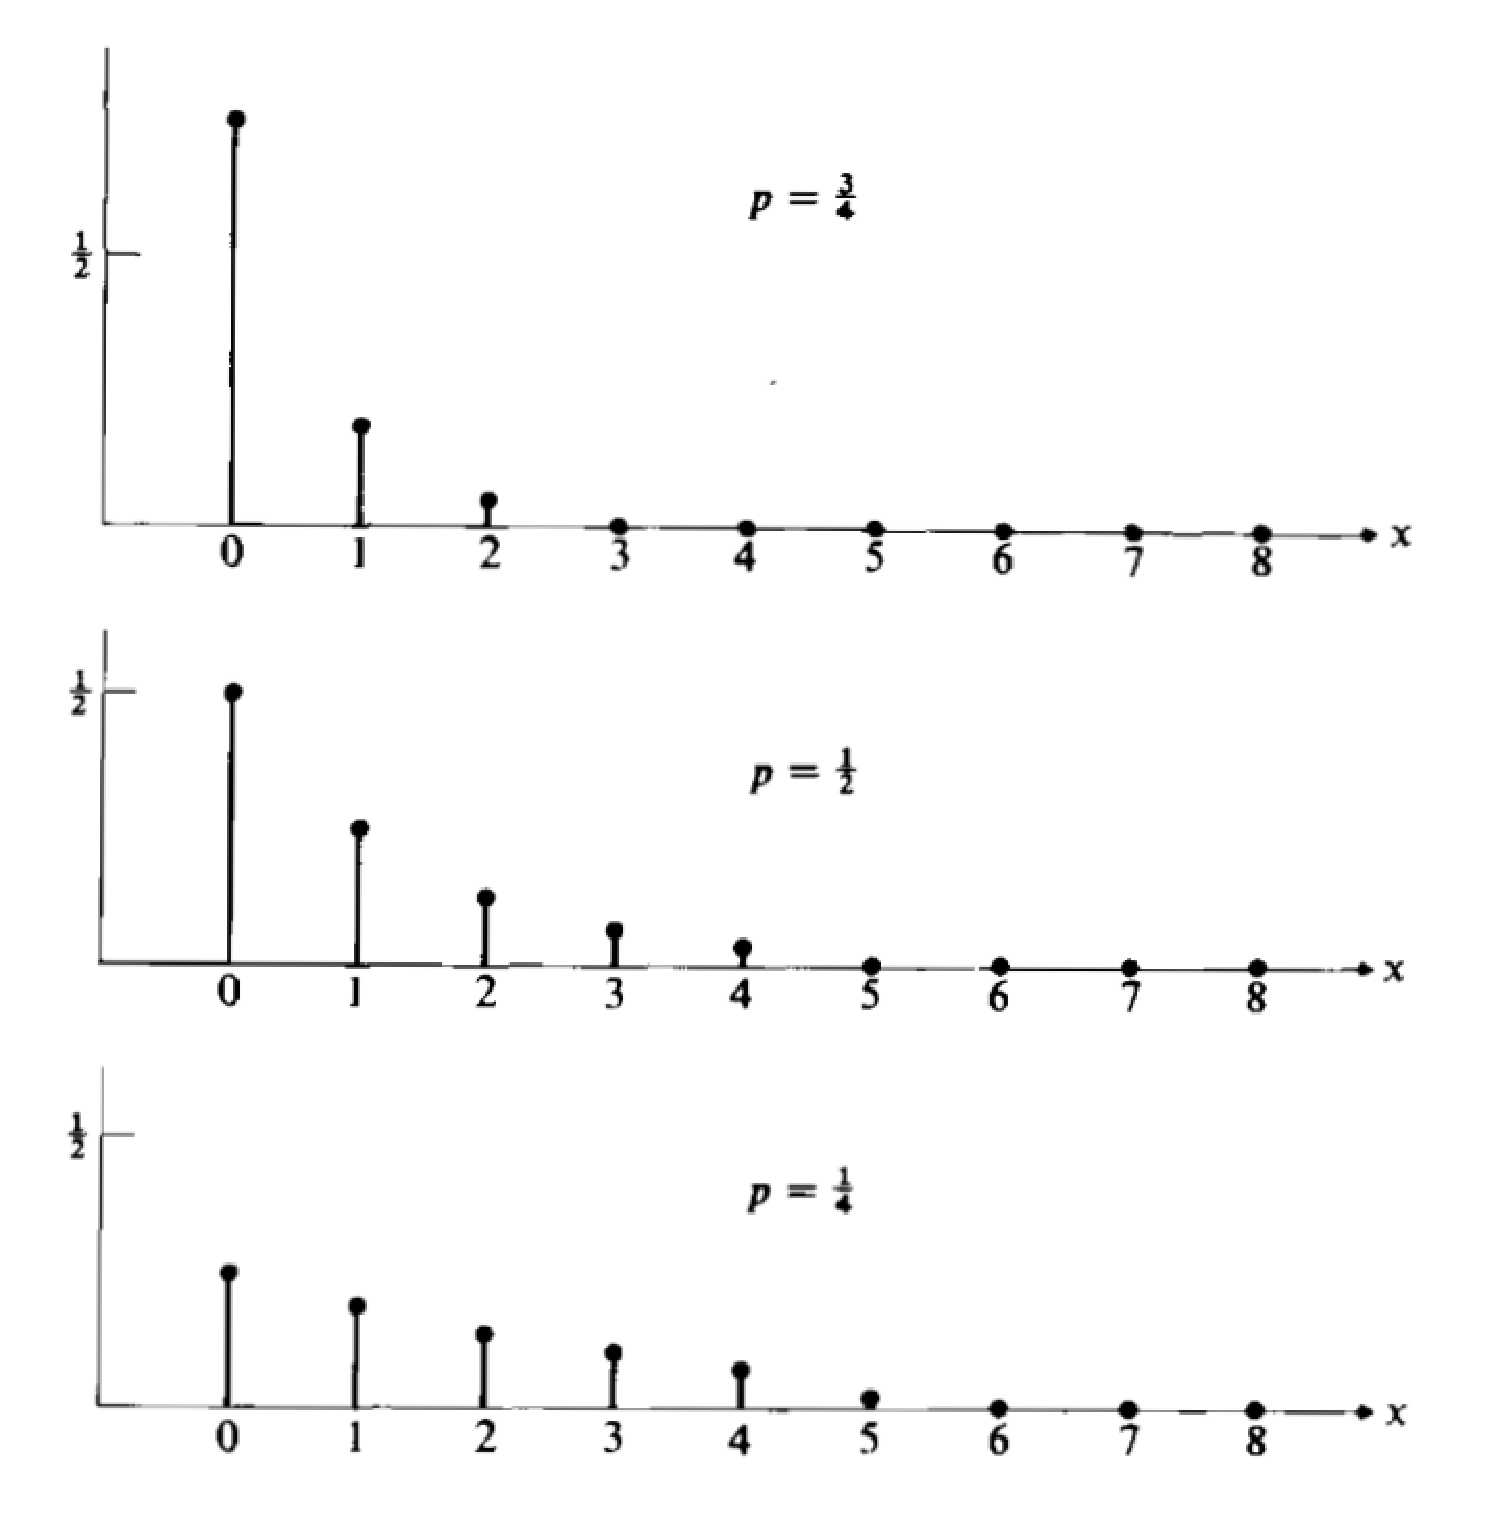
\includegraphics[scale = 0.3]{pictures/geometric_distribution.eps}
\caption{Pravděpodobnostní funkce geometrického rozdělení}
\label{geometric_distribution}
\end{figure}

\begin{theorem}
Jestliže náhodná veličina $X$ sleduje geometrické rozdělení, pak
\begin{gather*}
E[X] = \frac{q}{p}\\
D[X] = \frac{q}{p^2}\\
m(t) = \frac{p}{1 - qe^t}
\end{gather*}
\end{theorem}

\begin{proof}
Vzhledem k tomu, že geometrické rozdělení se speciální případ negitivního binomické rozdělení, odkazujeme se na příslušný důkaz pro negativní binomické rozdělení.
\end{proof}

\begin{theorem}
Jestliže náhodná veličina $X$ sleduje geometrické rozdělení, pak
\begin{equation*}
P[X \ge i + j | X \ge i] = P[x \ge j]~~~\textit{pro}~i,j = 0,1,2,...
\end{equation*}
\end{theorem}

\begin{proof}
\begin{gather*}
P[X \ge i + j|X \ge i] = \frac{P[X \ge i + 1]}{P[X \ge i]} = \frac{\sum_{x = i + j}^{\infty}p(1-p)^x}{\sum_{x=i}^{\infty}p(1-p)^x}\\
= \frac{(1 - p)^{i + j}}{(1 + p)^i} = (1-p)^j = P[X \ge j]
\end{gather*}
\end{proof}

\begin{example}
Uvažujme sérii vzájemně nezávislých Bernoulliho pokusů s pravděpodobostní úspěch $p$. Nechť náhodná veličina $X$ představuje počet neúspěšných pokusů, které předchází prvnímu úspěšnému pokusu. Pak sleduje náhodná veličina $X$ geometrické rozdělení.
\end{example}

\subsubsection{Negativní binomické rozdělení}

\begin{definition}[Negativní binomické rozdělení]
Jestliže náhodná veličina $X$ sleduje negativní binomické rozdělení, pak její pravděpodobnostní funkce má tvar
\begin{gather*}
f_X(x) =
\begin{cases}
\binom{r + x -1}{x} p^r q^x = \binom{-r}{x}p^r (-q)^r~~~\textit{pro}~x = 0, 1, 2,...\\
0~~~\textit{v ostatních případech}
\end{cases}\\
= \binom{r + x -1}{x}p^r q^x I_{\{0,1,2,...\}}(x)
\end{gather*}
kde $r = 1, 2, 3, ...$, $0 < p \le 1$ a $q = 1 - p$.
\end{definition}
Jestliže $r = 1$ pak se negativní binomické rozdělení zredukuje na geometrické rozdělení.

\begin{theorem}
Nechť má náhodná veličina $X$ negativní binomické rozdělení. Pak
\begin{gather*}
E[X] = \frac{rq}{p}\\
D[X] = \frac{rq}{p^2}\\
m(t) = \Big[\frac{p}{1 - qe^t} \Big]^r
\end{gather*}
\end{theorem}

\begin{proof}
\begin{gather*}
m(t) = E[e^{tX}] = \sum_{x = 0}^{\infty} e^{tx}\binom{-r}{x}p^r(-q)^x\\
= \sum_{x=0}^{\infty} \binom{-r}{x}p^r(-qe^t)^x = \Big[ \frac{p}{1 - qe^x} \Big]^r
\end{gather*}
kde jsme využili vztah
\begin{equation*}
(1 - x)^{-n} = \sum_{j = 0}^{\infty} \binom{-n}{j}(-x)^j = \sum_{j = 0}^{\infty} \binom{n + j - 1}{j} x^j~~~\textit{pro}~-1 < x < 1
\end{equation*}
Následnou derivací pak získáme
\begin{gather*}
m'(t) = p^r(-r)(1 - qe^t)^{-r-1}(-qe^t)\\
m''(t) = rqp^r \big[q(r+1)e^{2t}(1 - qe^t)^{-r-2} + e^t(1 - qe^t)^{-r-1} \big]
\end{gather*}
a proto
\begin{gather*}
E[X] = m'(t)\Big|_{t = 0} = \frac{rq}{p}\\
D[X] = m''(t)\Big|_{t = 0} - E[X]^2 = rqp^r[qp^{-r-2}(r+1) + p^{-r-1}] - \Big(\frac{rq}{p}\Big)^2\\
= \frac{rq^2}{p^2} + \frac{rq}{p} = \frac{rq}{p^2}
\end{gather*}
\end{proof}

\begin{example}
Uvažujme sérii vzájemně nezávislých Bernoulliho pokusů s pravděpodobností úspěchu $p$. Nechť náhodná veličina $X$ představuje počet neúspěšných pokusů, které předcházely $r$-tému úspěšnému pokusu. V tomto případě sleduje náhodná veličina $X$ negativní binomické rozdělení.

Odvození pravděpodobnostní funkce je následující. Poslední pokus musí skončit úspěchem. Mezi zbývajícími $x + r - 1$ pokusy musí být $x$ neúspěchů a $r - 1$ úspěchů, přičemž na jejich pořadí nezáleží. Výsledná pravděpodobnost je tak rovna
\begin{equation*}
\binom{x + r - 1}{r - 1}p^{r-1}q^x = \binom{r + x - 1}{x}p^{r-1}q^x
\end{equation*}
\end{example}

\subsection{Ostaní nespojitá rozdělení}

\subsubsection{Odvození ze stávajících rozdělení}

Jedním ze způsobů, jak vytvořit nová nespojitá rozdělení z výše uvedených, je pomocí ``seříznutí''. Pro ilustraci uvažujme Poissonovo rozdělení ``seříznuté'' v bodě 0. V některých situacích nemůže náhodná veličina nabývat hodnoty nula, avšak přesto se Poissonovo rozdělení zdá být vhodným modelem. Odpovídající pravděpodobnostní funkce pak má tvar
\begin{equation*}
f(x) =
\begin{cases}
\frac{e^{-\lambda} \lambda^x}{x!}\big(1 - e^{-\lambda} \big)~~~\textit{pro}~x = 1, 2, 3, ...\\
0~~~\textit{v ostatních případech}
\end{cases}
\end{equation*}
O takto odvozených pravděpodobnostních rozděleních hovoříme jako o zredukovaných pravděpodobnostních rozděleních.

Další způsob odvození nového typu nespojitého rozdělení opět ilustrujme na Poissonově rozdělení. Předpokládejme, že náhodná veličina $X$ sleduje Poissonovo rozdělení. Dále předpokládejme, že v rámci experimentu jsme, z určitých blíže nespecifikovaných důvodů, schopni rozlišit pouze žádnou, jednu nebo více než jednu realizaci. V tomto případě má pravděpodobnostní funkce tvar
\begin{equation*}
f(x) =
\begin{cases}
e^{-\lambda}~~~\textit{pro}~ x = 0\\
\lambda e^{-\lambda}~~~\textit{pro}~ x = 1\\
1 - e^{-\lambda} - \lambda e^{-\lambda}
\end{cases}
\end{equation*}
O náhodné velčině $X$ pak hovoříme jako o censorované náhodné veličině.

\subsubsection{Beta-binomické rozdělení}

\begin{definition}[Beta-binomické rozdělení]
Jestliže náhodná veličina $X$ sleduje beta-binomické rozdělení, pak její pravděpodobnostní funkce má tvar
\begin{equation*}
f(x) = \binom{n}{x} \frac{\Gamma(\alpha + \beta)}{\Gamma(\alpha) \Gamma(\beta)}\frac{\Gamma(x + \alpha) \Gamma(n + \beta - x)}{\Gamma(n + \alpha + \beta)}I_{\{0,1,...,n\}}(x)
\end{equation*}
kde $n$ je přirozené číslo větší než nula, $\alpha > 0$, $\beta > 0$ a $\Gamma(m)$ kde je tzv. gamma funkce
\begin{equation*}
\Gamma(m) = \int_0^{\infty}X^{m-1}e^{-x}dx,~~~ m > 0
\end{equation*}
Pro tuto náhodnou veličinu pak platí
\begin{gather*}
E[X] = \frac{n \alpha}{\alpha + \beta}\\
D[X] = \frac{n \alpha \beta (n + \alpha + \beta)}{(\alpha + \beta)^2(\alpha + \beta + 1)}
\end{gather*}
\end{definition}
Jestliže $\alpha = \beta = 1$, pak se beta-binomické rozdělení zredukuje na nespojité uniformní rozdělení.

\begin{definition}[Logaritmické rozdělení]
Jestliže náhodná veličina $X$ sleduje logaritmické rozdělení, pak její pravděpodobnostní funkce má tvar
\begin{gather*}
f(x) =
\begin{cases}
\frac{q^x}{-x \ln(p)}~~~\textit{pro}~x = 1, 2, ...\\
0~~~\textit{v ostatních případech}
\end{cases}\\
= \frac{q^x}{-x \ln(p)}I_{\{1, 2, ...\}}(x)
\end{gather*}
Pro tuto náhodnou veličinu pak platí
\begin{gather*}
E[X] = \frac{q}{-p \ln(p)}\\
D[X] = \frac{q(q + \ln(p))}{-\big(p \ln(p) \big)^2}
\end{gather*}
\end{definition}
Označení ``logaritmické rozdělení'' vychází ze skutečnosti, že odpovídající pravděpodobnostní funkce je rozvojem $\ln(1 - q)$. Logaritmické rozdělení lze odvodit jako limitní rozdělení negativního binomického rozdělení zobecněného pomocí parametru $r$, který představuje libovolné kladné číslo (nejen celé kladné číslo), a které je seříznuté v bodě 0.

\section{Spojité pravděpodobnostní rozdělení}

\subsection{Spojité uniformní rozdělení}

\begin{definition}[Spojité uniformní rozdělení]
Jestliže náhodná veličina $X$ sleduje spojité uniformní rozdělení, pak její pravděpodobnostní funkce má tvar
\begin{equation*}
f(x) = \frac{1}{b - a}I_{[a, b]}(x)
\end{equation*}
kde $-\infty < a < b < \infty$.
\end{definition}

\begin{figure}[htp]
\centering
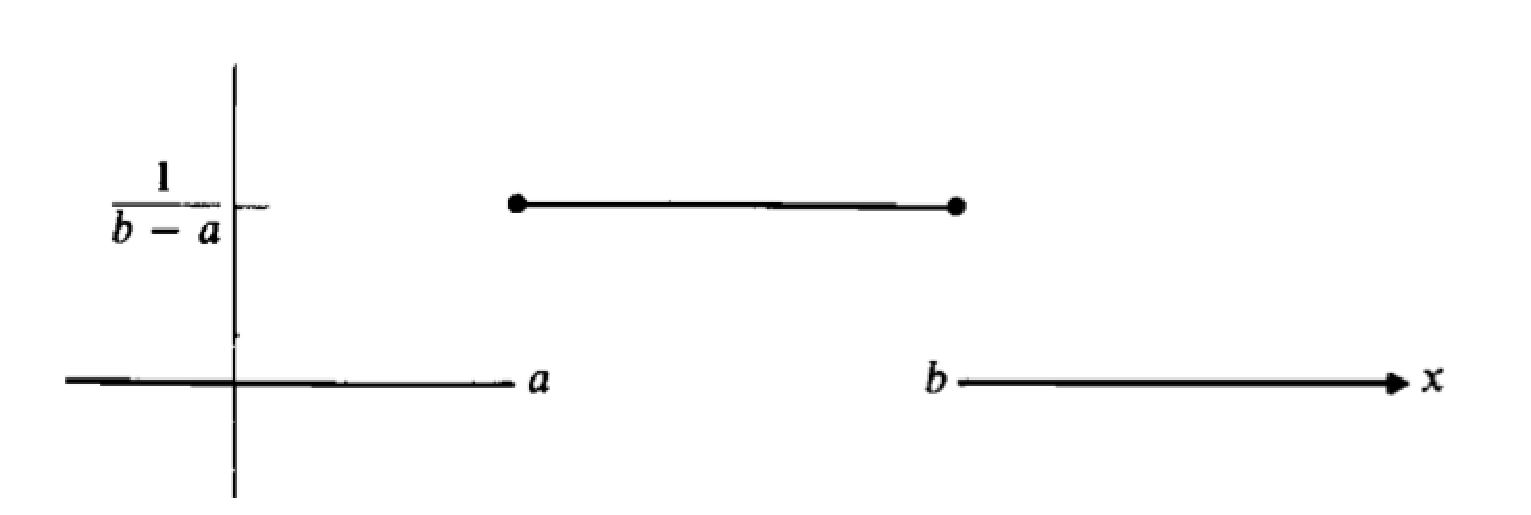
\includegraphics[scale = 0.5]{pictures/continuous_uniform_distribution.eps}
\caption{Pravděpodobnostní funkce spojitého uniformního rozdělení}
\label{continuous_uniform_distribution}
\end{figure}

\begin{theorem}
Jestliže má náhodná veličina $X$ spojité uniformní rozdělení, pak
\begin{gather*}
E[X] = \frac{a + b}{2}\\
D[X] = \frac{(b - a)^2}{12}\\
m(t) = \frac{e^{bt} - e^{at}}{(b - a)t}
\end{gather*}
\end{theorem}

\begin{proof}
\begin{gather*}
E[X] = \int_a^b x \frac{1}{b - a}dx = \frac{b^2 - a^2}{2(b - a)} = \frac{a + b}{2}\\
D[X] = E[X^2] - E[X]^2 = \int_a^b x^2 \frac{1}{b - a}dx - \Big(\frac{a + b}{2}\Big)^2\\
= \frac{b^3 - a^3}{3(b - a)} - \frac{(a + b)^2}{4} = \frac{(b - a)^2}{12}\\
m(t) = E[e^{tX}] = \int_a^b e^{tx} \frac{1}{b - a}dx = \frac{e^{bt} - e^{at}}{(b - a)t}
\end{gather*}
\end{proof}

\begin{theorem}
Kumulativní distribuční funkce spojitého uniformního rozdělení je
\begin{equation*}
F(x) = \frac{x - a}{b - a}I_{[a,b]}(x) + I_{(b, \infty)}(x)
\end{equation*}
\end{theorem}

Ačkoliv jsme definovali uniformní rozdělení nad uzavřeným intervalem $[a, b]$, lze toto rozdělení definovat nad intervalem $(a, b)$, $[a, b)$ nebo $(a,b]$. Pravděpodobnostní funkce bychom modifikovali do podoby $f(x) = \frac{1}{b - a}I_{(a, b)}(x)$, $f(x) = \frac{1}{b - a}I_{[a, b)}(x)$ resp. $f(x) = \frac{1}{b - a}I_{(a, b]}(x)$. Kumulativní distribuční funkce je však ve všech případech shodná.

\subsection{Normální rozdělení}

\begin{definition}[Normální rozdělení]
Jestliže náhodná veličina $X$ sleduje normální rozdělení, pak má její pravděpodobnostní funkce tvar
\begin{equation*}
f(x) = \frac{1}{\sqrt{2 \pi \sigma}} e^{-\frac{(x - \mu)^2}{2 \sigma^2}}
\end{equation*}
kde $-\infty < \mu < \infty$ a $\sigma > 0$. Jak ukážeme později, tyto parametry představuje střední hodnotu a směrodatnou odchylku tohoto pravděpodobnostního rozdělení.
\end{definition}

\begin{figure}[htp]
\centering
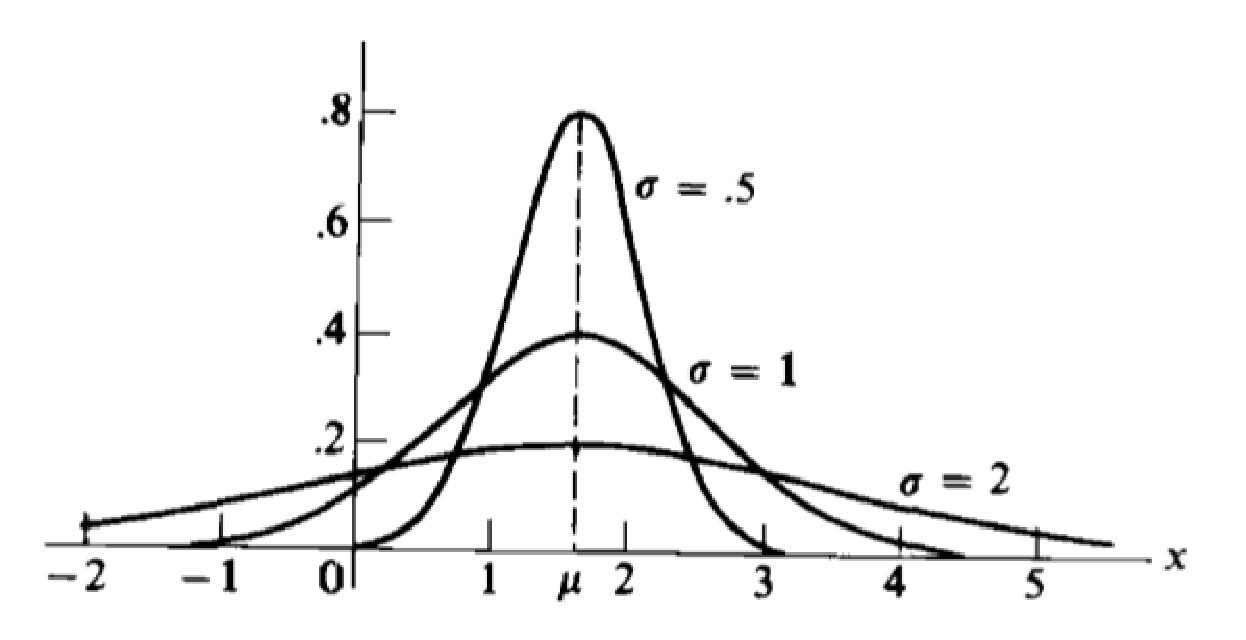
\includegraphics[scale = 0.5]{pictures/normal_distribution.eps}
\caption{Pravděpodobnostní funkce normálního rozdělení}
\label{normal_distribution}
\end{figure}

\begin{figure}[htp]
\centering
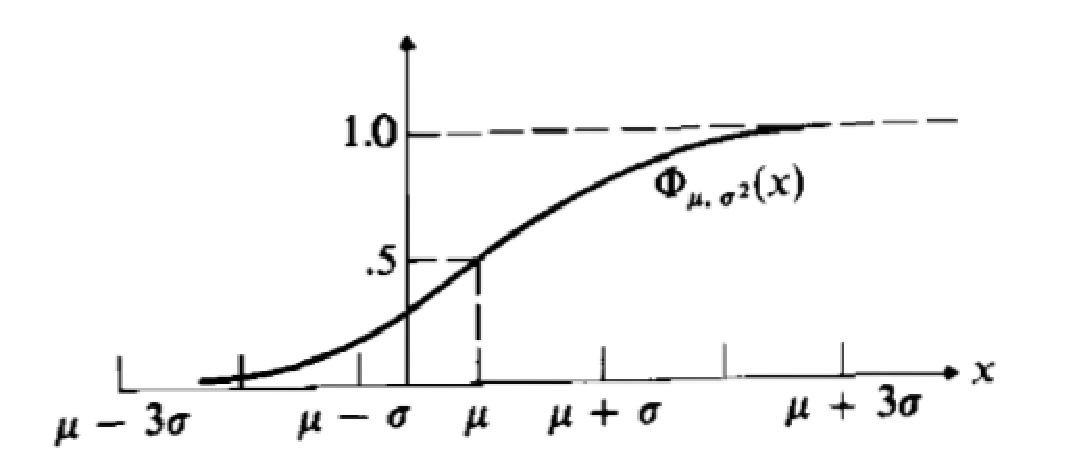
\includegraphics[scale = 0.5]{pictures/normal_cumulative_distribution.eps}
\caption{Kumulativní distribuční funkce normálního rozdělení}
\label{normal_cumulative_distribution}
\end{figure}   

Vzhledem k tomu, že normální rozdělení je velmi často používané, je pro jeho pravděpodobnostní funkci resp. kumulativní distribuční funkci používáno označení $\phi(\mu, \sigma^2)$ resp. $\Phi(\mu, \sigma^2)$. Jestliže $\mu = 0$ a $\sigma = 0$, hovoříme o tzv. standardizovaném popř. normalizovaném normálním rozdělení. V tomto případě se obvykle parametery v značení pravděpodobnostní a kumulativní distribuční funkce vypouštějí.

Protože je $\phi(\mu, \sigma^2)$ pravděpodobnostní funkcí, musí platit
\begin{equation*}
\int_{-\infty}^{\infty} \phi(\mu, \sigma^2)(x) dx = 1
\end{equation*}

\begin{proof}
Uvažujme neurčitý integrál
\begin{equation*}
A = \frac{1}{\sqrt{2 \pi} \sigma} \int_{-\infty}^{\infty} e^{-\frac{(x - \mu)^2}{2 \sigma^2}}dx
\end{equation*}
který lze s využitím substituce $y = \frac{x - \mu}{\sigma}$ upravit do tvaru
\begin{equation*}
A = \frac{1}{\sqrt{2 \pi}} \int_{-\infty}^{\infty} e^{-\frac{1}{2}y^2}dy
\end{equation*}
Potřebuje dokázat $A = 1$. Vzhledem k tomu, že $e^t$ je kladné pro všechna $t$, platí $A > 0$. Pokud bychom dokázali $A^2 = 1$, pak by to implikovalo $A = 1$. $A^2$ lze vyjádřit jako
\begin{gather*}
A^2 = \frac{1}{\sqrt{2 \pi}} \int_{-\infty}^{\infty} e^{-\frac{1}{2}y^2}dy \frac{1}{\sqrt{2 \pi}} \int_{-\infty}^{\infty} e^{-\frac{1}{2}z^2}dz\\
= \frac{1}{2 \pi} \int_{-\infty}^{\infty} \int_{-\infty}^{\infty} e^{-\frac{1}{2}(y^2 + z^2)}dydz
\end{gather*}
Následně tento integrál převedeme pomocí substitucí $y = r \sin(\theta)$ a $z = r \cos(\theta)$ do polárních souřadnic.
\begin{equation*}
A^2 = \frac{1}{2 \pi} \int_0^{\infty} \int_0^{2 \pi} r e^{-\frac{1}{2} r^2}d \theta dr = \int_0^{\infty} = r e^{-\frac{1}{2}r^2}dr = 1
\end{equation*}
\end{proof}

\begin{theorem}
Jestliže náhodná veličina $X$ sleduje normální rozdělení, pak
\begin{gather*}
E[X] = \mu\\
D[X] = \sigma^2\\
m(t) = e^{\mu + \sigma^2 t^2 / 2}
\end{gather*}
\end{theorem}
\begin{proof}
\begin{gather*}
m(t) = E[e^{tX}] = e^{t \mu}E[e^{t(X-\mu)}] = e^{t \mu} \int_{-\infty}^{\infty} \frac{1}{\sqrt{2 \pi}} e^{t(x-\mu)}e^{-(1/2\sigma^2)(x-\mu)^2}dx\\
= e^{t\mu} \frac{1}{\sqrt{2 \pi}} \int_{-\infty}^{\infty} e^{-(1/2 \sigma^2)[(x - \mu)^2 - 2 \sigma^2 t(x - \mu)]}dx
\end{gather*}
Jestliže doplníme kvadráty v závorkách
\begin{gather*}
(x - \mu)^2 - 2 \sigma^2 t(x - \mu) = (x - \mu)^2 - 2 \sigma^2 t(x - \mu) + \sigma^4 t^2 - \sigma^4 t^2\\
=(x - \mu - \sigma^2 t)^2 - \sigma^4 t^2
\end{gather*}
získáme
\begin{equation*}
m(t) = e^{t \mu} e^{\sigma^2 t^2 / 2} \frac{1}{\sqrt{2 \pi} \sigma} \int_{-\infty}^{\infty} e^{-(x - \mu - \sigma^2 t)^2 / 2 \sigma^2}dx
\end{equation*}
Integrál společně s členem $\frac{1}{\sqrt{2 \pi} \sigma}$ musí být roven 1, protože se jedná o plochu pod pravděpodobnostní funkcí normálního rozdělení se střední hodnotou $\mu + \sigma^2 t$ a rozptylem $\sigma^2$, a proto
\begin{equation*}
m(t) = e^{\mu t + \sigma^2 t^2 / 2}
\end{equation*}
Derivací $m(t)$ pro $t = 0$ získáme
\begin{gather*}
E[X] = m'(0) = \mu\\
D[X] = E[X^2] - E[X]^2 = m''(0) - \mu^2 = \sigma^2
\end{gather*}
\end{proof}

\begin{theorem}
Protože neurčitý integrál $\sigma_{\mu, sigma^2}(x)$ nelze řešit analyticky, jsme schopni kumulativní distribuční funkci prezentovat pouze ve tvaru
\begin{equation*}
\Phi_{\mu, \sigma^2}(x) = \int_{-\infty}^x \phi_{\mu, \sigma^2}(u)du
\end{equation*}
\end{theorem}
\begin{theorem}
Jestliže má náhodná veličina $X$ normální rozdělení, pak
\begin{equation*}
P[a < X < b] = \Phi \Big(\frac{b - \mu}{\sigma}\Big) - \Phi \Big(\frac{a - \mu}{\sigma}\Big)
\end{equation*}
\end{theorem}
\begin{proof}
\begin{gather*}
P[a < X < b] = \int_a^b \frac{1}{\sqrt{2 \pi} \sigma} e^{-\frac{1}{2}[(x - \mu)/\sigma]^2}dx\\
= \int_{(a - \mu)/\sigma}^{(b - \mu)/\sigma} \frac{1}{\sqrt{2 \pi}} e^{-\frac{1}{2}z^2}dz\\
= \Phi \Big(\frac{b - \mu}{\sigma}\Big) - \Phi \Big(\frac{a - \mu}{\sigma}\Big)
\end{gather*}
\end{proof}

\begin{theorem}
Velmi užitečným vztahem je
\begin{equation*}
\Phi(x) = 1 - \Phi(-x)
\end{equation*}
což vyplývá ze symetričnosti normálního rozdělení.
\end{theorem}

\begin{example}
Předpokládejme, že průměr strojově vyráběné kovové tyče má normální rozdělení se střední hodnotou 10 cm a směrodatnou odchylkou 0.1 cm. Aby mohla být tyč použita v navazující výrobě, musí být její průměr v rozmezí 9.9 až 10.2 cm. Jaké procento vyrobených tyčí splňuje tuto podmínku?

\begin{gather*}
P[9.9 < X < 10.2] = \Phi \Big(\frac{10.2 - 10}{0.1} \Big) - \Phi \Big(\frac{9.9 - 10}{0.1} \Big)\\
= \Phi(2) - \Phi(-1) \approx 0.9772 - 0.1587 = 0.8185
\end{gather*}
\end{example}

\subsection{Exponenciální a gamma rozdělení}

\subsubsection{Exponenciální rozdělení}

\begin{definition}[Exponenciální rozdělení]
Jestliže náhodná veličina $X$ sleduje exponenciální rozdělení, pak má její pravděpodobnostní funkce tvar
\begin{equation*}
f(x) = \lambda e^{- \lambda x}I_{[0, \infty)}(x)
\end{equation*}
kde $\lambda > 0$.
\end{definition}
\begin{theorem}
Jestliže náhodná veličina $X$ sleduje exponenciální rozdělení, pak
\begin{gather*}
E[X] = \frac{1}{\lambda}\\
D[X] = \frac{1}{\lambda^2}\\
m(t) = \frac{\lambda}{\lambda - t}
\end{gather*}
\end{theorem}

\begin{proof}
Vzhledem k tomu, že exponenciální rozdělení je specifickým případem gamma rozdělení, odkazujeme se na příslušný důkaz pro toto rozdělení.
\end{proof}

Jestliže lze v rámci určitého experimentu modelovat počet realizací za časovou jednotku pomocí Poissonova rozdělení, pak lze délku trvání jednotlivých realizací modelovat pomocí exponenciálního rozdělení.

\begin{theorem}
Jestliže náhodná veličina $X$ sleduje exponenciální rozdělení, pak
\begin{equation*}
P[x > a + b| X > a] = P[X > b]~~~\textit{pro}~a > 0 ~\textit{a}~ b > 0
\end{equation*}
\end{theorem}
\begin{proof}
\begin{equation*}
P[X > a + b | X > a] = \frac{P[X > a + b]}{P[X > a]} = \frac{e^{-\lambda(a + b)}}{e^{-\lambda a}} = e^{-\lambda b} = P[X > b]
\end{equation*}
\end{proof}

\subsubsection{Gamma distribuce}

\begin{definition}[Gamma rozdělení]
Jestliže náhodná veličina $X$ sleduje gamma rozdělení, pak má její pravděpodobnostní funkce tvar
\begin{equation*}
f(x) = \frac{\lambda}{\Gamma(r)}(\lambda x)^{r - 1}e^{-\lambda x}I_{[0, \infty)}(x)
\end{equation*}
kde $r > 0$, $\lambda > 0$ a $\Gamma(\cdot)$ je tzv. gamma funkce.
\end{definition}
Jestliže je parametr $r$ roven jedné, pak se gamma distribuce zredukuje na exponenciální rozdělení.

\begin{figure}[htp]
\centering
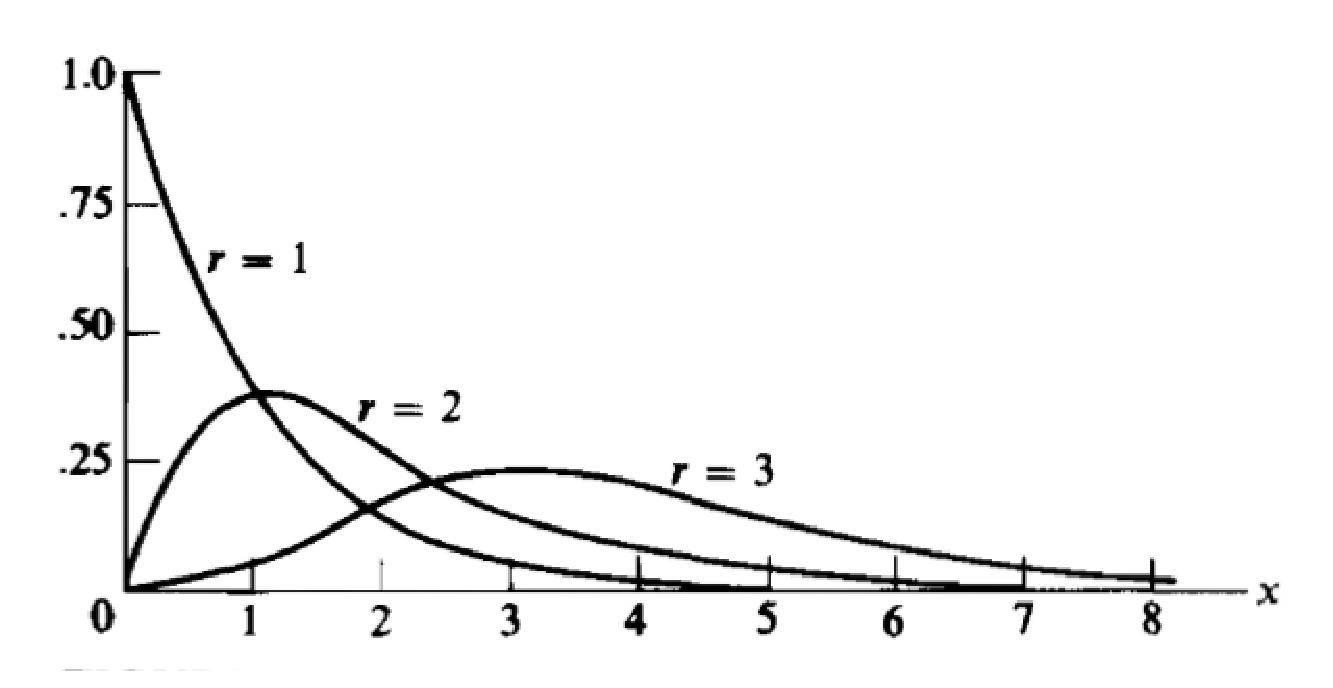
\includegraphics[scale = 0.5]{pictures/gamma_distribution.eps}
\caption{Pravděpodobnostní funkce gamma rozdělení}
\label{gamma_distribution}
\end{figure}

\begin{theorem}
Jestliže náhodná veličina $X$ sleduje gamma rozdělení, pak
\begin{gather*}
E[X] = \frac{r}{\lambda}\\
D[X] = \frac{r}{\lambda^2}\\
m(t) = \Big(\frac{\lambda}{\lambda - t} \Big)^r~~~\textit{pro}~t < \lambda
\end{gather*}
\end{theorem}
\begin{proof}
\begin{gather*}
m(t) = E[e^{tX}] = \int_0^{\infty} \frac{\lambda^r}{\Gamma(r)}e^{tx}x^{r-1}e^{-\lambda x} dx\\
= \Big(\frac{\lambda}{\lambda - t} \Big)^r \int_0^{\infty} \frac{(\lambda - t)^r}{\Gamma(r)}x^{r-1}e^{-(\lambda - t)x}dx = \Big( \frac{\lambda}{\lambda - t} \Big)^r
\end{gather*}
První a druhá derivace momentové funkce jsou pak
\begin{gather*}
m'(t) = r \lambda^r (\lambda - t)^{-r - 1}\\
m''(t) = r(r + 1)\lambda^r(\lambda - t)^{-r-2}
\end{gather*}
a proto
\begin{gather*}
E[X] = m'(0) = \frac{r}{\lambda}\\
D[X] = E[X^2] - E[X]^2 = m''(0) - \Big(\frac{r}{\lambda}\Big)^2 = \frac{r(r+1)}{\lambda^2} - \Big(\frac{r}{\lambda}\Big)^2 = \frac{r}{\lambda^2}
\end{gather*}
\end{proof}

Jestliže lze počet realizací v rámci určitého experimentu modelovat pomocí Poissonova rozdělení, pak lze délku časového úseku od okamžiku 0 do okamžiku $r$-té realizace modelovat pomocí gamma distribuce. Jedná se tedy o čas, který musíme čekat, než dojde k $r$-té realizaci.

\begin{theorem}
Jestliže náhodná veličina $X$ sleduje gamma rozdělení, kde parametr $r$ je kladné celé číslo, pak
\begin{equation*}
F(x) = 1 - \sum_{j = 0}^{r-1}\frac{e^{\lambda x}(\lambda x)^j}{j!}
\end{equation*}
\end{theorem}
\begin{proof}
Výše uvedenou větu lze dokázat postupným integrováním per partes.
\end{proof}

\subsection{Beta rozdělení}

\begin{definition}[Beta rozdělení]
Jestliže náhodná veličina $X$ sleduje beta rozdělení, pak její pravděpodobnostní funkce má tvar
\begin{equation*}
f(x) = \frac{1}{B(a,b)}x^{n-1}(1 - x)^{b - 1}I_{(0,1)}(x)
\end{equation*}
kde $a > 0$, $b > 0$ a $B(a, b) = \int_0^1 x^{a - 1}(a1 - x)^{b - 1}dx$ je tzv. beta funkce.
\end{definition}

Pro $a = b$ se beta rozdělení zredukuje na spojité uniformní rozdělení nad intervalem $(0, 1)$.

\begin{figure}[htp]
\centering
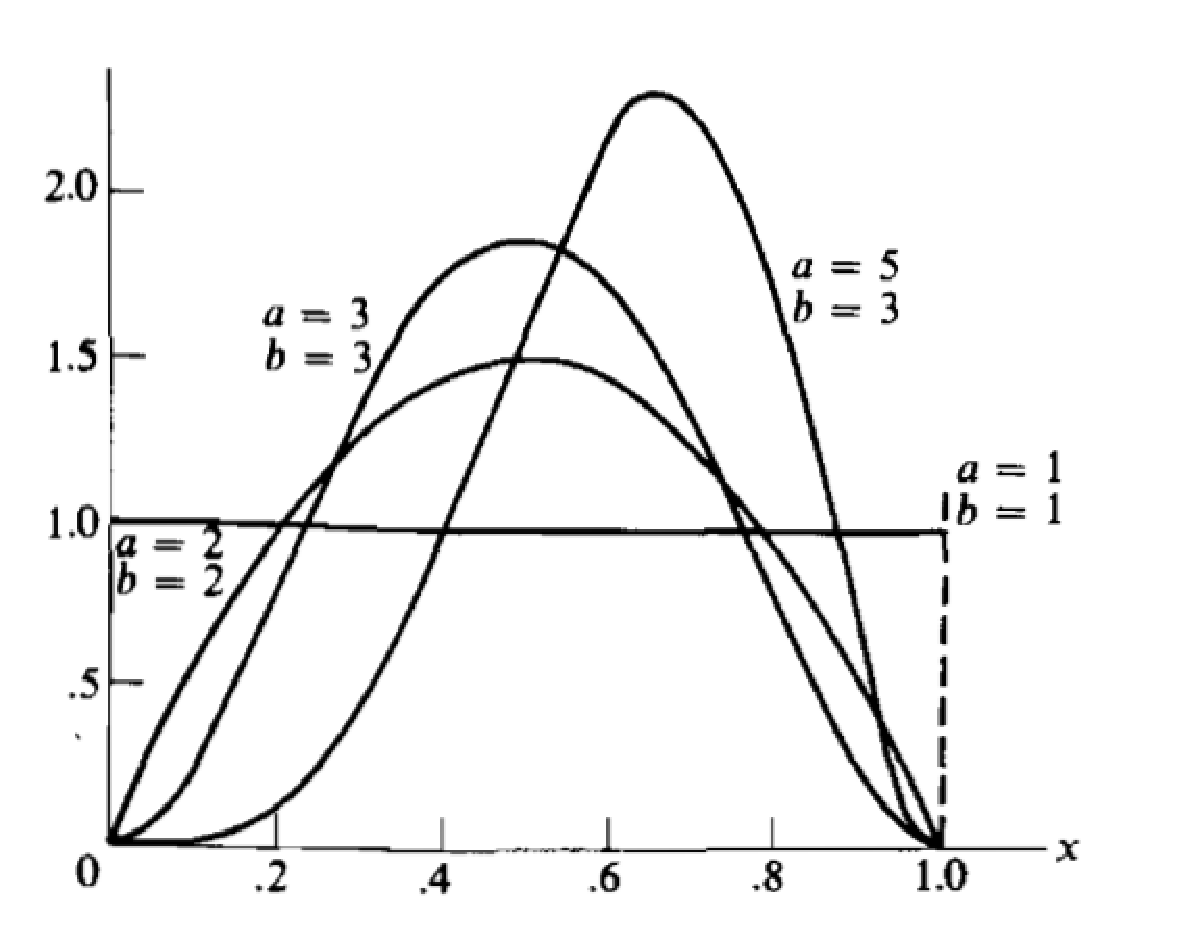
\includegraphics[scale = 0.5]{pictures/beta_distribution.eps}
\caption{Pravděpodobnostní funkce beta rozdělení}
\label{beta_distribution}
\end{figure}

\begin{theorem}
Kumulativní distribuční funkce náhodné veličiny $X$ s beta rozdělením má tvar
\begin{equation*}
F(x) = I_{(0, 1)}(x) \int_0^x \frac{1}{B(a, b)}u^{a - 1}(1 - u)^{b - 1}du + I_{[1, \infty)}(x)
\end{equation*}
\end{theorem}

Momentová funkce beta rozdělení nemá jednoduchou analytickou formu, nicméně momenty lze snadno odvodit přímo z jejich definice, tj. bez použití momentové funkce.

\begin{theorem}
\begin{gather*}
E[X] = \frac{a}{a + b}\\
D[X] = \frac{ab}{(a + b + 1)(a + b)^2}
\end{gather*}
\end{theorem}
\begin{proof}
\begin{gather*}
E[X^k] = \frac{1}{B(a, b)} \int_0^1 x^{k + a - 1}(1 - x)^{b - 1}dx\\
=\frac{B(k + a, b)}{B(a, b)} = \frac{\Gamma(k + a)\Gamma(b)}{\Gamma(k + a + b)} \frac{\Gamma(a + b)}{\Gamma(a) \Gamma(b)}\\
= \frac{\Gamma(k + a)\Gamma(a + b)}{\Gamma(a) \Gamma(k + a + b)}
\end{gather*}
Proto
\begin{gather*}
E[X] = \frac{\Gamma(a + 1) \Gamma(a + b)}{\Gamma(a) \Gamma(a + b + 1)} = \frac{a}{a + b}\\
D[X] = E[X^2] - E[X]^2 = \frac{\Gamma(a + 2)\Gamma(a + b)}{\Gamma(a) \Gamma(a + b + 2)} - \Big(\frac{a}{a + b}\Big)^2\\
= \frac{(a + 1)a}{(a + b + 1)(a + b)} - \Big(\frac{a}{a + b}\Big)^2 = \frac{ab}{(a + b + 1)(a + b)^2}
\end{gather*}
\end{proof}

Beta rozdělení nabývá na intervalu $(0, 1)$ kladných hodnot a její pravděpodobnostní funkce je charakteristická velkým množstvím tvarů.

\section{Ostatní spojitá rozdělení}

V této kapitole budou představena některá další spojitá rozdělení. Studentovo, chi-kvadrát a F rozdělení budou představena později.

\subsection{Cauchyho rozdělení}

\begin{definition}[Cauchyho rozdělení]
Jestliže náhodná veličina $X$ sleduje Cauchyho rozdělení, pak její pravděpodobnostní funkce má tvar
\begin{equation*}
f(x) = \frac{1}{\pi \beta \big(1 + \big(\frac{x - a}{\beta} \big)^2 \big)}
\end{equation*}
kde $-\infty < \alpha < \infty$ a $\beta > 0$.
\end{definition}
Cauchyho rozdělení je symetrické okolo parametru $\alpha$, avšak střední hodna a vyšší momenty nejsou definovány.

\begin{theorem}
Kumulativní distribuční funkce Cauchyho rozdělení má tvar
\begin{gather*}
F(x) = \frac{1}{\pi} \int_{-\infty}^x \frac{1}{\pi \beta \big(1 + \big(\frac{u - a}{\beta}\big)^2 \big)}du\\
= \frac{1}{2} + \frac{1}{\pi}arctan \Big( \frac{x - \alpha}{\beta}\Big)
\end{gather*}
\end{theorem}

\subsection{Lognormální rozdělení}

\begin{definition}[Lognormální rozdělení]
Nechť je $X$ kladná náhodná veličina a definujme novou náhodnou veličinu $Y = \ln(X)$. Sleduje-li $Y$ normální rozdělení, pak sleduje $X$ lognormální rozdělení. Pravděpodobnostní funkce lognormálního rozdělení má tvar
\begin{equation*}
f(x) = \frac{1}{x \sqrt{2 \pi} \sigma}e^{-\frac{1}{2 \sigma^2}(\ln(x) - \mu)^2}I_{(0, \infty)}(x)
\end{equation*}
kde $-\infty < \mu < \infty$ a $\sigma > 0$.
\end{definition}

\begin{theorem}
Jestliže náhodná veličina $X$ sleduje lognormální rozdělení, pak
\begin{gather*}
E[X] = e^{\mu + \frac{1}{2}\sigma^2}\\
D[X] = e^{2 \mu + 2 \sigma^2} - e^{2\mu + \sigma^2}
\end{gather*}
\end{theorem}

Jestliže má $X$ lognormální rozdělení, pak $E[\ln(X)] = \mu$ a $D[\ln(X)] = \sigma^2$.

\subsection{Laplaceova distribuce}

\begin{definition}[Laplaceova distribuce]
Jestliže náhodná veličina $X$ sleduje Laplaceovo rozdělení, pak má její pravděpodobnostní funkce tvar
\begin{equation*}
f(x) = \frac{1}{2 \beta} e^{-\frac{|x - \alpha|}{\beta}}
\end{equation*}
kde $-\infty < \alpha < \infty$ a $\beta > 0$.
\end{definition}

\begin{theorem}
Jestliže náhodná veličina $X$ sleduje Laplaceovo rozdělení, pak
\begin{gather*}
E[X] = \alpha\\
D[X] = 2 \beta^2
\end{gather*}
\end{theorem}

\subsection{Weibullovo rozdělení}

\begin{definition}
Jestliže náhodná veličina $X$ sleduje Weibullovo rozdělení, pak její pravděpodobnostní funkce má tvar
\begin{equation*}
f(x) = abx^{b-1}e^{-ax^b}I_{(0, \infty)}(x)
\end{equation*}
kde $a > 0$ a $b > 0$.
\end{definition}

\begin{theorem}
Jestliže náhodná veličina $X$ sleduje Weibullovo rozdělení, pak
\begin{gather*}
E[X] = \frac{1}{a}^{\frac{1}{b}}\Gamma(1 + b^{-1})\\
D[X] = \frac{1}{a}^{\frac{2}{b}}\big(\Gamma(1 + 2 b^{-1}) - \Gamma^2(1 + b^{-1}) \big)
\end{gather*}
\end{theorem}

Pro $b = 1$ se Weibullovo rozdělení zredukuje na exponenciální rozdělení.

\subsection{Logistické rozdělení}

\begin{definition}[Logistické rozdělení]
Jestliže náhodná veličina $X$ sleduje logistické rozdělení, pak má její kumulativní distribuční funkce tvar
\begin{equation*}
F(x) = \frac{1}{1 + e^{- \frac{x - \alpha}{\beta}}}
\end{equation*}
kde $-\infty < \alpha < \infty$ a $\beta > 0$.
\end{definition}

\begin{theorem}
Jestliže náhodná veličina $X$ sleduje logistické rozdělení, pak
\begin{gather*}
E[X] =  \alpha\\
D[X] = \frac{\beta^2 \pi^2}{3}
\end{gather*}
\end{theorem}

Pro kumulativní distribuční funkci logistického rozdělení platí $F(\alpha - d) = 1 - F(\alpha + d)$, a pravděpodobnostní funkce je tak symetrická kolem parametru $\alpha$.

\subsection{Paretovo rozdělení}

\begin{definition}[Pareto rozdělení]
Jestliže náhodná veličina $X$ sleduje Paretovo rozdělení, pak má její pravděpodobnostní funkce tvar
\begin{equation*}
f(x) = \frac{\theta}{x_0} \Big(\frac{x_0}{x}\Big)^{\theta + 1}I_{(x_0, \infty)}(x)
\end{equation*}
kde $\theta > 0$ a $x_0 > 0$.
\end{definition}

\begin{theorem}
Jestliže náhodná veličina $X$ sleduje Paretovo rozdělení, pak
\begin{gather*}
E[X] = \frac{\theta x_0}{\theta - 1}~~~ \textit{pro}~ \theta > 0\\
D[X] = \frac{\theta x_0^2}{\theta - 2} - \Big(\frac{\theta x_0}{\theta - 1} \Big)^2 ~~~ \textit{pro}~  > 2
\end{gather*}
\end{theorem}

\section{Poznámky}

\subsection{Aproximace}

Ačkoliv existuje celá řada aproximací jednoho rozdělení pomocí jiného, budeme se v této kapitole zabývat pouze třemi z nich. Některé další aproximace představíme v kapitole o Centrální limitní větě.

\subsubsection{Aproximace binomického rozdělení Poissonovým rozdělením}

Pravděpodobnostní funkce binomického rozdělení má tvar
\begin{equation*}
\binom{n}{x}p^x(1 - p)^{n-x}~~~\textit{pro}~x = 0, 1, ..., n
\end{equation*}
Jestliže se $n$ blíží nekonečnu a $p$ se blíží nule, přičemž $np = \lambda$ zůstává konstantní, pak
\begin{equation*}
\binom{n}{x}p^x(1 - p)^{n-x} \rightarrow \frac{e^{-\lambda} \lambda^x}{x!}
\end{equation*}
pro fixní celé číslo $x$. Výše uvedený vztah vyplývá z
\begin{gather*}
\binom{n}{x}p^x(1 - p)^{n - x} = \frac{(n)_x}{x!}\Big(\frac{\lambda}{n}\Big)^x \Big(1 - \frac{\lambda}{n} \Big)^{n-x}\\
= \frac{\lambda^x}{x!} \frac{(n)_x}{n^x}\Big(1 - \frac{\lambda}{n}\Big)^n\Big(1 - \frac{\lambda}{n} \Big)^{-x} \rightarrow \frac{e^{-\lambda}\lambda^x}{x!}
\end{gather*}
protože
\begin{gather*}
\lim_{n \rightarrow \infty}\frac{(n)_x}{n^x} = 1\\
\lim_{n \rightarrow \infty}\Big(1 - \frac{\lambda}{n}\Big)^{-x} = 1\\
\lim_{n \rightarrow \infty}\Big(1 - \frac{\lambda}{n} \Big)^n = e^{-\lambda}
\end{gather*}
Proto pro dostatečně velká $n$ a malá $p$ lze tedy binomickou pravděpodobnost $\binom{n}{x}p^x(1 - p)^{n-x}$ aproximovat pomocí Poissonovy pravděpodobnosti $\frac{e^{-np}(np)^x}{x!}$.

\subsubsection{Aproximace binomického a Poissonova rozdělení normálním rozdělením}

\begin{theorem}
Nechť náhodná veličina $X$ sleduje Poissonovo rozdělení. Pak pro fixní $a < b$ platí
\begin{equation*}
P\Big[a < \frac{X - \lambda}{\sqrt{\lambda}}\Big] = P[\lambda + a\sqrt{\lambda} < X < \lambda + b\sqrt{\lambda}] \rightarrow \Phi(b) - \Phi(b) ~~~\textit{pro}~ \lambda \rightarrow \infty
\end{equation*}
\end{theorem}

\begin{theorem}[De Moivre-Laplaceova limitní věta]
Nechť náhodná veličina $X$ sleduje binomické rozdělení. Pak pro fixní $a < b$ platí
\begin{equation*}
P\Big[a \le \frac{X - np}{\sqrt{npq}} \le b \Big] = P[np + a \sqrt{npq} \le X \le np + b \sqrt{npq}] \rightarrow \Phi{b} - \Phi(a) ~~~\textit{pro}~ n \rightarrow \infty
\end{equation*}
\end{theorem}

\begin{example}
Uvažujme hrací kostku, která je vržena 600 krát. Nechť náhodná veličina $X$ představuje počet hodů, při kterých padla šestka. Je zřejmé, že $X$ sleduje binomické rozdělení s $n = 600$ a $p = \frac{1}{6}$ a že $E[X] = 100$. Nalezněte pravděpodobnost $P[90 \le X \le 110]$.

Platí
\begin{equation*}
P[90 \le X \le 110] = \sum_{j = 90}^{110}\binom{600}{j}\Big(\frac{1}{6}\Big)^j \Big(\frac{5}{6}\Big)^{600 - j}
\end{equation*}
S využitím aproximace se lze vyhnout rutinnímu výpočtu.
\begin{gather*}
P[90 \le X \le 110] \approx \Phi\Big(\frac{110 - 100}{\sqrt{\frac{500}{6}}}\Big) - \Phi\Big(\frac{90 - 100}{\sqrt{\frac{500}{6}}}\Big)\\
=\Phi \Big(\sqrt{\frac{6}{5}}\Big) - \Phi \Big(\sqrt{-\frac{6}{5}}\Big) \approx \Phi(1.095) - \Phi(-1.095) \approx 0.726
\end{gather*}
\end{example}

\subsection{Vztah mezi Poissonovým a exponenciálním rozdělením}

V předchozím textu jsme ukázali, že Poissonovo rozdělení je vhodné pro modelování počtu vzájemně nezávislých realizací v čase. Předpokládejme, že k jedné takovéto realizaci došlo, a že předmětem našeho zájmu je délka, po kterou budeme muset čekat, než dojde k další realizaci. Pravděpodobnost
\begin{equation*}
P[X > x] = P[\textit{žádná realizace v časovém intervalu délky x}] = e^{-vx}
\end{equation*}
kde $v$ je střední míra realizace. Proto
\begin{equation*}
F(x) = P[X \le x] = 1 - P[X > x] = 1 - e^{-vx} ~~~\textit{pro}~x > 0
\end{equation*}
což znamená, že $X$ má exponenciální rozdělení. Tento vztah platí také naopak. Lze dokázat, že lze-li dobu mezi vzájemně nezávislými realizacemi modelovat pomocí exponenciálního rozdělení, pak lze počet realizací modelovat pomocí Poissonova rozdělení.

\subsection{Smíšená pravděpodobnostní rozdělení}

Uvažujme pravděpodobnostní funkce $f_0(\cdot), f_1(\cdot), ..., f_n(\cdot)$, které jsou všechny buďto spojité nebo nespojité. Dále uvažujme parametry $p_0, p_1, ..., p_n$ které splňují
\begin{gather*}
p_i \ge 0\\
\sum_{i = 0}^{\infty}p_i = 1
\end{gather*}
Pak $\sum_{i = 0}^{\infty}p_i f_i(x)$ představuje pravděpodobnostní funkcí, která vznikla ``smícháním'' pravděpodobnostních funkcí $f_0(\cdot), f_1(\cdot), ..., f_n(\cdot)$.

\begin{example}
Ilustrujme myšlenku smíšeného pravděpodobnostního rozdělení s pomocí pravděpodobnostních funkcí $f_0(x) = \phi(\mu_0, \sigma_0^2)(x)$ a $f_1(x) = \phi(\mu_1, \sigma_1^2)(x)$. Pak
\begin{gather*}
p_0 \phi(\mu_0, \sigma_0^2)(x) + p_1 \phi(\mu_1, \sigma_1^2)(x)\\
= (1 - p) \frac{1}{\sqrt{2 \pi \sigma_0}}e^{-\frac{1}{2}(\frac{x - \mu_0}{\sigma_0})^2} + p \frac{1}{\sqrt{2 \pi \sigma_1}}e^{-\frac{1}{2}(\frac{x - \mu_1}{\sigma_1})^2}
\end{gather*}
\end{example}

Výše uvedené smíšené rozdělení nazýváme smíšeným normálním rozdělením. V našem konkrétním případě má toto rozdělení pět parametrů, což mu umožňuje nabývat nejrůznějších tvarů. Vhodným nastavením parametrů lze tak vytvořit např. bimodální rozdělení, tj. rozdělení se dvěma vrcholy. Díky své flexibilitě je tak ``míchání'' pravděpodobnostních rozdělení často využíváno při modelování některých experimentů.

Koncept smíšeného pravděpodobnostního rozdělení lze dále rozšířit. Nechť $\{f(x; \theta)\}$ představuje rodinu pravděpodobnostních funkcí indexovaných parametrem $\theta$. Množinu všech hodnot, kterých může $\theta$ nabývat, označme $\Theta$. Je-li $\Theta$ interval a $g(\theta)$ pravděpodobnostní funkce, která je nulová pro všechny prvky mimo $\Theta$, pak
\begin{equation*}
\int_{\Theta}f(x; \theta) g(\theta) d\theta
\end{equation*}
je opět pravděpodobnostní funkce.

\begin{example}
Uvažujme $f(x; \theta) = \frac{e^{-\theta}\theta^x}{x!}$ pro $x = 0, 1, 2, ...$ a $f(x; \theta) = 0$ v ostatních případech. Dále uvažujme pravděpodobnostní funkci gamma rozdělení $g(\theta) = \frac{\lambda^r}{\Gamma(r)}\theta^{r-1}e^{-\lambda \theta}I_{(0, \infty)}(\theta)$. Pak
\begin{gather*}
\int_0^{\infty}f(x;\theta)g(\theta)d\theta = \int_0^{\infty} \frac{e^{-\theta}\theta^x}{x!} \frac{\lambda^r}{\Gamma(r)}\theta^{r - 1}e^{-\theta \lambda} d \theta = \frac{\lambda^r}{x! \Gamma(r)} \int_0^{\infty} \theta^{r + x - 1} e^{-(\lambda + 1)\theta}d \theta\\
= \frac{\lambda^r}{x! \Gamma(r)} \frac{\Gamma(r + x)}{(\lambda + 1)^{r + x}}\int_0^{\infty} \frac{[(\lambda + 1)\theta]^{r + x - 1} e^{-(\lambda + 1)\theta}}{\Gamma(r + x)} d[(\lambda + 1)\theta]\\
= \Big(\frac{\lambda}{\lambda + 1}\Big)^r \frac{\Gamma(r + x)}{x!\Gamma(r)}\frac{1}{(\lambda + 1)^x}\\
= \binom{r + x - 1}{x}\Big(\frac{\lambda}{\lambda + 1}\Big)^r\Big(\frac{1}{\lambda + 1}\Big)^x ~~~\textit{pro}~x = 0, 1, 2, ...
\end{gather*}
což je pravděpodobnostní funkce binomického rozdělení s parametery $r$ a $p = \frac{\lambda}{\lambda + 1}$. Na binomické rozdělení je tak možné nahlížet jako na gamma smíšené Poissonovo rozdělení.
\end{example}

\subsection{Zredukovaná pravděpodobnostní rozdělení}

Pro ilustraci uvažujme normální rozdělení ``seříznuté'' zleva hodnotou 0 a zprava hodnotou 1. Pravděpodobnostní funkce takovéhoto zredukovaného pravděpodobnostního rozdělení je
\begin{equation*}
f(x) = \frac{\phi(\mu, \sigma^2)(x)I_{(0,1)}(x)}{\Phi(\mu, \sigma^2)(1) - \Phi(\mu, \sigma^2)(0)}
\end{equation*}

Obecná definice zredukovaného spojitého pravděpodobnostního rozdělení je následující.

\begin{theorem}
Jestliže $X$ je spojitá náhodna veličina s pravděpodobnostní funkcí $f(\cdot)$ a kumulativní distribuční funkcí $F(\cdot)$, pak pravděpodobnostní funkce náhodné veličiny $X$ zredukované na interval $(a, b)$ je
\begin{equation*}
\frac{f(x)I_{(a, b)}(x)}{F(b) - F(a)}
\end{equation*}
\end{theorem}

\chapter{Vícero náhodných proměnných}

\section{Sdružená pravděpodobnost}

\subsection{Sdružená kumulativní distribuční funkce}

\begin{definition}[Sdružená kumulativní distribuční funkce]
Nechť jsou $X_1, X_2, ..., X_k$ náhodné veličiny definované nad pravděpodobnostním prostorem $(\Omega, \mathscr{A}, P[\cdot])$. Sdružená kumulativní distribuční funkce $F_{X_1, ..., X_k}(\cdot, ..., \cdot)$ je definována jako $P[X_1 \le x_1, ..., X_k \le x_k]$ pro všechna $x_1, x_2, ..., x_k$.
\end{definition}

Sdružená kumulativní distribuční funkce je tak funkcí s definičním oborem $R^k$ a intervalem $[0, 1]$ jako oborem hodnot.

\subsubsection{Dvourozměrná sdružená kumulativní distribuční funkce}

\begin{theorem}
Dvourozměrná sdružená kumulativní distribuční funkce splňuje následující podmínky.
~
\begin{enumerate}
\item
\begin{gather*}
F(-\infty, y) = \lim_{x \rightarrow -\infty}F(x, y) = 0 ~~~\textit{pro všechna}~y\\
F(x, -\infty) = \lim_{y \rightarrow -\infty}F(x, y) = 0 ~~~\textit{pro všechna}~x\\
F(\infty, \infty) = \lim_{x \rightarrow \infty, y \rightarrow \infty}F(x, y) = 1
\end{gather*}
\item Jestliže $x_1 < x_2$ a $y_1 < y_2$, pak $P[x_1 < X \le x_2, y_1 < Y \le y_2] = F(x_2, y_2) - F(x_2, y_1) - F(x_1, y_2) + F(x_1, y_1) \ge 0$.
\item Funkce $F(x,y)$ je v obou parametrech zprava spojitá. To znamená, že $\lim_{0 < h \rightarrow 0}F(x + h, y) = \lim_{0 < h \rightarrow 0}F(x, y + h) = F(x, y)$.
\end{enumerate}
\end{theorem}

\begin{definition}[Dvourozměrná kumulativní distribuční funkce]
Libovolná funkce, která splňuje výše uvedené tři podmínky, je dvourozměrnou kumulativní distribuční funkcí.
\end{definition}

\begin{definition}[Marginální kumulativní distribuční funkce]
Jestliže je $F_{X,Y}(\cdot, \cdot)$ sdruženou kumulativní distribuční funkcí náhodných veličin $X$ a $Y$, pak kumulativní distribuční funkce $F_X(\cdot)$ a $F_Y(\cdot)$ jsou její marginální kumulativní distribuční funkce.
\end{definition}

\begin{corollary}
Platí $F_X(x) = F_{X,Y}(x, \infty)$ a $F_Y(y) = F_{X,Y}(\infty, y)$. Známe-li sdruženou kumulativní distribuční funci, jsme schopni určit také odpovídající marginální kumulativní distribuční funkce. 
\end{corollary}

Obrácené tvrzení však neplatí - znalost marginálních kumulativních distribučních funkcí neimplikuje znalost sdružené kumulativní distribuční funkce.

\begin{theorem}
V případě dvourozměrné sdružené kumulativní distribuční funkce pro všechna $x$ a $y$ platí
\begin{equation*}
F_X(x) + F_Y(y) - 1 \le F_{X,Y}(x,y) \le \sqrt{F_X(x)F_Y(y)}
\end{equation*}
\end{theorem}

\begin{proof}
Nejprve dokážeme
\begin{equation*}
F_X(x) + F_Y(y) - 1 \le F_{X,Y}(x,y)
\end{equation*}
Levou stranu této nerovnosti lze upravit do podoby
\begin{gather*}
1 - P[x < X < \infty, y < Y < \infty] + F_{X,Y} - 1\\
= F_{X,Y} - P[x < X < \infty, y < Y < \infty]
\end{gather*}
Protože $P[x < X < \infty, y < Y < \infty] \ge 0$, platí $F_X(x) + F_Y(y) - 1 \le F_{X,Y}(x,y)$. Následně dokážeme
\begin{equation*}
F_{X,Y}(x,y) \le \sqrt{F_X(x)F_Y(y)}
\end{equation*}
Tuto nerovnost lze upravit do podoby
\begin{gather*}
\ln \big(F_{X,Y}(x,y) \big) + \ln \big( F_{X,Y}(x,y) \big) \le \ln \big(F_x(x) \big) + \ln \big( F_Y(y) \big)
\end{gather*}
Protože $F_{X,Y}(x,y) \le F_X(x)$ a $F_{X,Y}(x,y) \le F_Y(y)$, výše uvedená nerovnost platí, čímž uzavíráme důkaz.
\end{proof}

\subsection{Sdružená pravděpodobnostní funkce nespojité náhodné veličiny}

Jestliže jsou $X_1, X_2, ..., X_k$ náhodné veličiny definované nad shodným pravděpodobnostním prostorem, pak je $(X_1, X_2, ..., X_k)$ $n$-rozměrnou náhodnou veličinou.

\begin{definition}[Sdružená nespojitá náhodná veličina]
Náhodná veličina $(X_1, X_2, ..., X_k)$ je $k$-rozměrnou nespojitou náhodnou veličinou, jestliže může nabývat hodnot pouze nad spočetným množstvím bodů $(x_1, x_2, ..., x_k)$ z $R^k$.
\end{definition}

\begin{definition}[Sdružená nespojitá pravděpodobnostní funkce]
Jestliže $(X_1, X_2, ..., X_k)$ je $k$-rozměrná nespojitá náhodná veličina, pak její sdružená nespojitá pravděpodobnostní funkce $f_{X_1, X_2, ..., X_k}(\cdot, ..., \cdot)$ je definována pro hodnoty $(x_1, x_2, ..., x_k)$, kterých může náhodná veličina $(X_1, X_2, ..., X_k)$ nabývat, jako
\begin{equation*}
f_{X_1, X_2, ..., X_k} = P[X_1 = x_1, X_2 = x_2, ..., X_k = x_k]
\end{equation*}
V ostatních případech je tato funkce rovna nule.
\end{definition}
Stejně jako v případě jednorozměrné náhodné veličiny také v případě $k$-rozměrné náhodné veličiny platí $\sum f_{X_1, X_2, ..., X_k}(x_1, x_2, ..., x_k) = 1$, kde sčítáme přes všechny přípustné hodnoty náhodné veličiny $(X_1, X_2, ..., X_k)$.

\begin{theorem}
Jestliže $X$ a $Y$ jsou sdruženě nespojité náhodné veličiny, pak znalost $F_{X,Y}(\cdot, \cdot)$ je ekvivalentní znalosti $f_{X,Y}(\cdot, \cdot)$. Toto tvrzení lze zobecnit také na $k$-rozměrnou náhodnou veličinu.
\end{theorem}

\begin{proof}
Nechť $(x_1, y_1), (x_2, y_2), ...$ představují všechny možné hodnoty náhodné veličiny $(X, Y)$. Jestliže známe $f_{X,Y}$, pak
\begin{equation*}
F_{X,Y}(x,y) = \sum f_{X,Y}(x_i, y_i)
\end{equation*}
kde sčítáme přes všechna $i$, pro která $x_i \le x$ a $y_i \le y$. Naopak je-li dáno $F_{X,Y}(\cdot, \cdot)$ pro všechna $(x_i, y_i)$, pak
\begin{equation*}
f_{X,Y}(x_i, y_i) = F_{X,Y}(x_i, y_i) - \lim_{0 < h \rightarrow 0} F_{X,Y}(x_i - h, y_i) - \lim_{0 < h \rightarrow 0}F_{X,Y}(x_i, y_i - h)
\end{equation*}
\end{proof}

\begin{definition}[Marginální nespojitá pravděpodobnostní funkce]
Jestliže jsou $X$ a $Y$ sdružené nespojité náhodné veličiny, pak $f_X(\cdot)$ a $f_Y(\cdot)$ představují marginální pravděpodobnostní funkce. Tuto definici lze zobecnit. Nechť $X_{i_1}, ..., X_{i_m}$ představují libovolnou podmnožinu sdružených nespojitých náhodných veličin $X_1, ..., X_k$. Pak $f_{X_{i_1}, ..., X_{i_m}}(x_{i_1}, ..., x_{i_m})$ představuje marginální pravděpodobnostní funkci. 
\end{definition}

Jestliže jsou $X_1, ..., X_k$ sdružené nespojité náhodné veličiny, pak lze libovolnou marginální pravděpodobnostní funkci odvodit ze sdružené pravděpodobnostní funkce. Obrácené tvrzení však neplatí.

\begin{example}
Uvažujme hod dvěma čtyřstěny. Náhodná veličina $X$ značí hodnotu hodu prvního z nich. Náhodná veličina $Y$ pak značí největší z obou hodů. Předpokládejme, že tyto čtyřstěny nejsou dokonale vyvážené, a proto se skutečně realizované pravděpodobnosti liší od očekávaných. Jednu z možných situací zachycuje následující tabulka.
\begin{center}
  \begin{tabular}{|c|c|c|c|c|}
    \hline
    $4$ & $1/16 + \epsilon$ &  $1/16 - \epsilon$ & $1/16$ & $4/16$\\
    \hline
    $3$ & $1/16 - \epsilon$ &  $1/16 + \epsilon$ & $3/16$ & $0$\\
    \hline
    $2$ & $1/16$ &  $2/16$ & $0$ & $0$\\
    \hline
    $1$ & $1/16$ &  $0$ & $0$ & $0$\\
    \hline
    $y/x$ & $1$ & $2$ & $3$ & $4$\\
    \hline
  \end{tabular}
\end{center}
Pro libovolné $0 \le \epsilon \le \frac{1}{16}$ definuje tato tabulka sdruženou pravděpodobnostní funkci. Nicméně marginální pravděpodobnosti jsou nezávislé na $\epsilon$. Tento příklad tedy ilustruje, že znalost marginálních pravděpodobnostních funkcí neimplikuje znalost sdružené pravděpodobnostní funkce.
\end{example}

Uvažujme experiment, který má $k+1$ možných výsledků. Označme tyto výsledky jako $s_1, s_2, ...,s_{k+1}$. Definujme $p_i = P[s_i]$ pro $i = 1, ..., k+1$. Je zřejmé, že musí platit $\sum_{i = 1}^{k + 1}p_i = 1$. Předpokládejme, že tento pokus opakujeme $n$-krát a že jednotlivé pokusy jsou vzájemně nezávislé. Nechť náhodná velčina $X_i$ představuje počet realizací $s_i$. Nespojitá pravděpodobnostní funkce náhodných veličin $X_1, ..., X_k$ je definována jako
\begin{equation*}
f_{X_1, ..., X_k}(x_1, ..., x_k) = \frac{n!}{\prod_{i = 1}^{k + 1}x_i!}\prod_{i = 1}^{k + 1}p_i^{x_i}
\end{equation*}
kde $x_i = 0, ..., n$ a $\sum_{i = 1}^{k + 1} x_i = n$. Všimněme si, že platí $X_{k+1} = n - \sum_{i = 1}^k X_i$.

Výše uvedenou rovnici lze vysvětlit následovně. Levou stranu této rovnice je možné vyjádřit ve tvaru $P[X_1 = x_1, ..., X_{k + 1} = x_{k + 1}]$. Zajímá nás tak pravděpodobnost, že mezi $n$ vzájemně nezávislými pokusy bude právě $x_1$ realiací $s_1$,  $x_2$ realizací $s_2$ až $x_{k + 1}$ realiací $s_{k + 1}$, kde $\sum_1^{k+1}x_i = n$. Za předpokladu nezávislosti jednotlivých pokusů lze pravděpodobnost jednoho takovéhoto uspořádání vyjádřit jako $p_1^{x_1}p_2^{x_2} \cdots p_{k+1}^{x_k + 1}$. Takovýchto uspořádání pak existuje $\frac{n!}{x_1!x_2! \cdots x_{k+1}!}$.

\begin{definition}[Multinomiální rozdělení]
Výše uvedená sdružená nespojitá pravděpodobnostní funkce se nazývá multinomiální distribucí.
\end{definition}

Multinomiální rozdělení má $(k + 1)$ parametrů a to $n, p_1, p_2, ..., p_k$. Parametr $p_{k+1}$ je definován jako $1 - p_1 - p_2 - ... - p_k$. Marginální rozdělení náhodné veličiny $X_i$ má charakter binomického rozdělení s parametry $n$ a $p_i$, protože na výsledek každého experimentu je možné pohlížet jako realizaci popř. nerealizaci výsledku $s_i$. Na každý z $n$ pokusů je tak možné pohlížet jako na Bernoulliho pokus a na sérii $n$ pokusů je pak možné modelovat pomocí binomického rozdělení.

\subsection{Sdružená pravděpodobnostní funkce spojité náhodné veličiny}

\begin{definition}[Sdružená spojitá náhodná veličina a její pravděpodobnostní funkce]
$k$-rozměrná náhodná veličina $(X_1, X_2, ..., X_k)$ je $k$-rozměrnou náhodnou veličinou právě tehdy a jen tehdy, jestliže existuje funkce $f_{X_1, ..., X_k}(\cdot, ..., \cdot) \ge 0$ taková, že
\begin{equation*}
F_{X_1, ..., X_k}(x_1, ..., x_k) = \int_{-\infty}^{x_k} \cdots \int_{-\infty}^{x_1} f_{X_1, ..., X_k}(u_1, ..., u_k)du_1 \cdots du_k
\end{equation*}
pro všechna $(x_1, ..., x_k)$. Funkce $f_{X_1, ..., X_k}(\cdot, ..., \cdot)$ je tzv. sdruženou pravděpodobnostní funkcí. Tato funkce splňuje následující dvě podmínky.
\begin{enumerate}
\item $f_{X_1, ..., X_k}(x_1, ..., x_k) \ge 0$
\item $\int_{-\infty}^{\infty} \cdots \int_{-\infty}^{\infty} f_{X_1, ..., X_k}(x_1, ..., x_k)dx_1 \cdots dx_k = 1$
\end{enumerate}
\end{definition}

\begin{example}
Uvažujme funkci
\begin{equation*}
f(x,y) = K(x + y)I_{(0, 12)}(x)I_{(0,1)}(y)
\end{equation*}
Lze vhodně zvolit konstantu $K$ tak, aby tato funkce byla dvourozměrnou pravděpodobnostní funkcí?

\begin{gather*}
\int_{-\infty}^{\infty} \int_{-\infty}^{\infty} K(x + y)dx dy = K \int_0^1 \int_0^1 (x + y)dx dy\\
=K \int_0^1 \big(\frac{1}{2} + y \big)dy = K \big(\frac{1}{2} + \frac{1}{2} \big) = 1
\end{gather*}
pro $K = 1$. Proto je funkce $f(x,y) = (x + y) I_{(0,1)}(x)I_{(0,1)}(y)$ sdruženou pravděpodobnostní funkcí.
\end{example}

\begin{theorem}
Jestliže jsou $X$ a $Y$ sdružené spojité náhodné veličiny, pak znalost sdružené kumulativní distribuční funkce $F_{X,Y}(\cdot, \cdot)$ je ekvivalentní znalosti sdružené pravděpodobnostní funkce $f_{X,Y}(\cdot, \cdot)$. Tuto větu lze rozšířit také na $k-$rozměrné spojité náhodné veličiny.
\end{theorem}
\begin{proof}
Pro danou sdruženou pravděpodobnostní funkci $f_{X,Y}(\cdot, \cdot)$ lze pro libovolné $(x,y)$ odvodit sdruženou kumulativní distribuční funkci $F_{X,Y}(x,y)$ jako
\begin{equation*}
F_{X,Y}(x,y) = \int_{-\infty}^y \int_{-\infty}^x f_{X,Y}(u,v)du dv
\end{equation*}
Naopak, pro danou sdruženou kumulativní distribuční funkci $F_{X,Y}(x,y)$ lze odpovídající sdruženou pravděpodobnostní funkci $f_{X,Y}(\cdot, \cdot)$ odvodit jako
\begin{equation*}
f_{X,Y}(x,y) = \frac{\partial^2 F_{X,Y}(x,y)}{\partial x \partial y}
\end{equation*}
kde $x$ a $y$ představují body, pro které je $F_{X,Y}(x,y)$ derivovatelná.
\end{proof}

\begin{definition}[Marginální pravděpodobnostní funkce]
Jestliže jsou $X$ a $Y$ sdružené spojité náhodné veličiny, pak $f_X(\cdot)$ a $f_Y(\cdot)$ jsou nazývány marginálními pravděpodobnostními funkcemi.

Tuto definici lze zobecnit. Nechť $X_{i_1}, ..., X_{i_m}$ představuje libovolnou podmnožinu sdružených náhodných veličin $X_1, ..., X_k$. Pak je funkce $f_{X_{i_1}, ..., X_{i_m}}(x_{i_1}, ..., x_{i_m})$ je nazývána marginální pravděpodobnostní funkcí náhodné veličiny $(X_{i_1}, ..., X_{i_m})$.
\end{definition}

Jestliže jsou $X$ a $Y$ sdružené spojité náhodné veličiny, pak platí
\begin{equation*}
f_X(x) = \int_{-\infty}^{\infty} f_{X,Y}(x,y)dy
\end{equation*}
a
\begin{equation*}
f_Y(y) = \int_{-\infty}^{\infty} f_{X,Y}(x,y)dx
\end{equation*}
protože
\begin{equation*}
f_X(x) = \frac{d F_X(x)}{dx} = \frac{d}{dx}\Big[\int_{-\infty}^x \Big(\int_{-\infty}^{\infty}f_{X,Y}(u,y)dy \Big) du \Big] = \int_{-\infty}^{\infty} f_{X,Y}(x,y)dy
\end{equation*}
a
\begin{equation*}
f_Y(y) = \frac{d F_Y(y)}{dy} = \frac{d}{dy}\Big[\int_{-\infty}^x \Big(\int_{-\infty}^{\infty}f_{X,Y}(x,u)dx \Big) du \Big] = \int_{-\infty}^{\infty} f_{X,Y}(x,y)dx
\end{equation*}

\begin{example}
Uvažujme sdruženou pravděpodobnostní funkci
\begin{equation*}
f_{X,Y}(x,y) = (x + y)I_{(0,1)}(x) I_{(0, 1)}(y)
\end{equation*}
Sdruženou kumulativní distribuční funkci lze vypočíst následujícím způsobem.
\begin{gather*}
F_{X,Y}(x,y) = I_{(0,1)}(x) I_{(0, 1)}(y) \int_0^y \int_0^x (u + v)du dv + I_{(0,1)}(x)I_{[1, \infty)}(y) \int_0^1 \int_0^x (u + v)du dv\\
+ I_{[1, \infty)}(x)I_{(0,1)}(y) \int_0^y \int_0^1 (u + v) du dv + I_{[1, \infty)}(x)I_{[1, \infty)}(y)\\
= \frac{1}{2}[(x^2y + xy^2)I_{(0,1)}(x)I_{(0,1)}(y) + (x^2 + x)I_{(0, 1)}(x)I_{[1, \infty)}(y)\\
+ (y + y^2)I_{[1, \infty)}(x)I_{(0, 1)}(y)] + I_{[1, \infty)}(x)I_{[1, \infty)}(y)
\end{gather*}
Marginální pravděpodobnostní funkci pak lze vyjádřit jako
\begin{gather*}
f_X(x) = \int_{-\infty}^{\infty} f_{X,Y}(x,y)dy = I_{(0, 1)}(x) \int_0^1(x+y)dy = \big(x + \frac{1}{2} \big)I_{(0, 1)}(x)
\end{gather*}
popř. jako
\begin{gather*}
f_X(x) = \frac{\partial F_{X,Y}(x, \infty)}{\partial x} = \frac{\partial F_X(x)}{\partial x} = I_{(0,1)}(x) \frac{\partial}{\partial x} \Big(\frac{x^2 + x}{2} \Big) = \big(x + \frac{1}{2} \big)I_{(0, 1)}(x)
\end{gather*}
\end{example}

\section{Podmíněné rozdělení a nezávislost}

\subsection{Podmíněná kumulativní distribuční funkce nespojité náhodné veličiny}

\begin{definition}[Podmíněná nespojitá pravděpodobnostní funkce]
Nechť jsou $X$ a $Y$ sdružené nespojité náhodné veličiny se sdruženou nespojitou pravděpodobnostní funkcí $f_{X,Y}(\cdot, \cdot)$. Podmíněná nespojitá pravděpodobnostní funkce $f_{Y|X}(\cdot | x)$ náhodné veličiny $Y$ pro $X = x$ je definována jako
\begin{equation*}
f_{Y|X}(y|x) = \frac{f_{X,Y}(x,y)}{f_X(x)}
\end{equation*}
je-li $f_X(x) > 0$, kde $f_X(x)$ je marginální pravděpodobnostní funkce náhodné veličiny $X$ v bodě $x$. Pro $f_X(x) = 0$ není funkce $f_{Y|X}(\cdot | x)$ definována. Podobně
\begin{equation*}
f_{X|Y}(x|y) = \frac{f_{X,Y}(x,y)}{f_Y(y)}
\end{equation*}
za podmínky $f_Y(y) > 0$.
\end{definition}

Protože náhodné veličiny $X$ a $Y$ jsou nespojité, mohou nabývat hodnot některého z bodů koncentrace $x_1, x_2,...$ v případě $X$ a $y_1, y_2, ...$ v případě $Y$. Jestliže $f_X(x) > 0$, pak $x = x_i$ pro některé $i$ a $f_X(x_i) = P[X = x_i]$. Analogicky $f_{X,Y}(x_i, y_i) = P[X = x_i, Y = y_j]$. Proto
\begin{equation*}
f_{Y|X}(y_j|x_i) = \frac{f_{X,Y}(x_i, y_j)}{f_X(x_i)} = \frac{P[X = x_i, Y = y_j]}{P[X = x_i]} = P[Y = y_j | X = x_i]
\end{equation*}
Jedná se tedy o podmíněnou pravděpodobnost, tak jak jsme ji definovali v první kapitole.

Vzhledem k tomu, že $f_{Y|X}(y_j|x_i)$ je nespojitá distribuční funkce, musí být kladná a její součet přes všechny přípustné hodnoty $Y$ musí být roven jedné. První podmínka je splněna, protože $f_{X,Y}(x,y)$ je nezáporné a $f_X(x)$ je kladné, a proto je jejich podíl kladný. Druhá podmínka je taktéž splněna, protože
\begin{equation*}
\sum_j f_{Y|X}(y_j|x) = \sum_j \frac{f_{X,Y}(x, y_j)}{f_X(x)} = \frac{1}{f_X(x)} \sum_j f_{X,Y}(x,y_j) = \frac{f_X(x)}{f_X(x)} = 1
\end{equation*} 

\begin{definition}[Podmíněná nespojitá kumulativní distribuční funkce]
Jestliže jsou $X$ a $Y$ sdružené nespojité náhodné veličiny, pak podmíněná nespojitá kumulativní distribuční fukce $F_{Y|X}(\cdot | x)$ je definována jako $F_{Y|X}(y|x) = P[Y \le y | X = x]$ pro $f_X(x) > 0$. Vazba mezi podmíněnou nespojitou kumulativní distribuční funkcí a pravděpodobnostní funkcí je dána vztahem
\begin{equation*}
F_{Y|X}(y|x) = \sum_{j:y_j \le y} f_{Y|X}(y_j | x)
\end{equation*}
\end{definition}

\begin{definition}[Podmíněná nespojitá pravděpodobnostní funkce]
Nechť $(X_1, ..., X_k)$ je $k$-rozměrná nespojitá náhodná veličina a nechť $X_{i_1}, ..., X_{i_r}$ a $X_{j_1}, ..., X_{j_s}$ jsou dvě neslučitelné podmnožiny náhodných veličin $X_1, ..., X_k$. Podmíněná pravděpodobnostní funkce $r$-rozměrné náhodné veličiny $X_{i_1}, ..., X_{i_r}$ pro dané hodnoty $(x_{j_1}, ..., x_{j_s})$ náhodné veličiny $X_{j_1}, ..., X_{j_s}$ je definována jako
\begin{gather*}
f_{X_{i_1}, ..., X_{i_r}|x_{j_1},...,x_{j_s}}(x_{i_1}, ..., x_{i_r}|x_{j_1}, ..., x_{j_s})\\
= \frac{f_{X_{i_1}, ..., X_{i_r}, X_{j_i}, ..., X_{j_s}}(x_{i_1}, ..., x_{i_r}, x_{j_1}, ..., x_{j_s})}{f_{X_{j_1}, ..., X_{j_s}}(x_{j_1}, ..., x_{j_s})}
\end{gather*}
\end{definition}

\begin{example}
Vyberme 12 karet bez vracení ze standardního hracího balíčku. Nechť $X_1$ představuje počet tažených es, $X_2$ představuje počet tažených dvojek, $X_3$ představuje počet tažených trojek a $X_4$ počet tažených čtyřek. Sdružená pravděpodobnostní funkce těchto čtyř náhodných veličin je
\begin{equation*}
f_{X_1, X_2, X_3, X_4}(x_1, x_2, x_3, x_4) = \frac{\binom{4}{x_1}\binom{4}{x_2}\binom{4}{x_3}\binom{4}{x_4}\binom{36}{12 - x_1 - x_2 - x_3 - x_4}}{\binom{52}{12}}
\end{equation*}
kde $x_i = 0, 1, 2, 3, 4$ při omezení $\sum x_i \le 12$. Existuje velké množství souvisejících podmíněných pravděpodobnostních funkcí. Jednou z nich je např.
\begin{gather*}
f_{X_2, X_4 | X_1, X_3}(x_2, x_4 | x_1, x_3)\\
= \frac{\binom{4}{x_1}\binom{4}{x_2}\binom{4}{x_3}\binom{4}{x_4}\binom{36}{12 - x_1 - x_2 - x_3 - x_4} \Big/ \binom{52}{12}}{\binom{4}{x_1}\binom{4}{x_3}\binom{44}{12 - x_1 - x_3} \Big/ \binom{52}{12}}\\
= \frac{\binom{4}{x_2}\binom{4}{x_4}\binom{36}{12 - x_1 - x_2 - x_3 - x_4} \Big/ \binom{52}{12}}{\binom{44}{12 - x_1 - x_3} \Big/ \binom{52}{12}}
\end{gather*}
\end{example}

\subsection{Podmíněná pravděpodobnostní funkce spojitých náhodných veličin}

\begin{definition}[Podmíněná pravděpodobnostní funkce]
Nechť jsou $X$ a $Y$ sdružené spojité náhodné veličiny se sdruženou pravděpodobnostní funkcí $f_{X,Y}(x,y)$. Podmíněná pravděpodobnostní funkce náhodné veličiny $Y$ pro $X = x$ je definována jako
\begin{equation*}
f_{Y|X}(y|x) = \frac{f_{X,Y}(x,y)}{f_X(x)}
\end{equation*}
kde $f_X(x) > 0$. Pro $f_X(x) > 0$ není tato funkce definována. Podobně $f_{X|Y}(x|y)$ je definována jako
\begin{equation*}
f_{X|Y}(x|y) = \frac{f_{X,Y}(x,y)}{f_Y(y)}
\end{equation*}
pro $f_Y(y) > 0$ a nedefinováno pro $f_Y(y) = 0$.
\end{definition}

Funkce $f_{Y|X}(\cdot | x)$ se nazývá podmíněná pravděpodobnostní funkce a proto by měla být nezáporná a její integrál přes všechny přípustné hodnoty by měl být roven jedné. První podmínka je splněna, protože $f_{X,Y}(x,y)$ je nezáporné a $f_Y(y)$ je kladné. Druhá podmínka je taktéž splněna, protože
\begin{gather*}
\int_{-\infty}^{\infty} f_{Y|X}(y|x)dy = \int_{-\infty}^{\infty} \frac{f_{X,Y}(x,y)}{f_X(x)}dy\\
= \frac{1}{f_X(x)} \int_{-\infty}^{\infty} f_{X,Y}(x,y)dy = \frac{f_X(x)}{f_X(x)} = 1
\end{gather*}

Uvažujme $f_{Y|X}(\cdot | x_0)$. Funkci $f_{X,Y}(x,y)$ lze znároznit jako plochu nad rovinou $xy$. Rovina kolmá na rovinu $xy$, která ji protíná v přímce $x = x_0$, protíná plochu $f_{X,Y}(x,y)$ v křivce $f_{X,Y}(x_0,y)$. Plocha pod toutu křivkou je
\begin{equation*}
\int_{-\infty}^{\infty}f_{X,Y}(x_0, y)dy = f_X(x_0)
\end{equation*}
Proto, vydělíme-li $f_{X,Y}(x_0,y)$ touto plochou $f_X(x_0)$, získáme pravděpodobnostní funkce $f_{Y|X}(y|x_0)$.

\begin{definition}[Podmíněná spojitá kumulativní distribuční funkce]
Jestliže jsou $X$ a $Y$ sdružené spojité náhodné veličiny, pak je podmíněná kumulativní distribuční funkce náhodné veličiny $Y$ pro $X = x$ definována jako
\begin{equation*}
F_{Y|X}(y|x) = \int_{-\infty}^y f_{Y|X}(z|x)dz
\end{equation*}
pro všechna taková $x$, kde $f_X(x) > 0$.
\end{definition}

\begin{example}
Uvažujme sdruženou pravděpodobnostní funkci
\begin{equation*}
f_{X,Y}(x,y) = (x + y)I_{(0,1)}(x)I_{(0,1)}(y)
\end{equation*}
Podmíněnou pravděpodobnostní funkci pak lze vypočíst jako
\begin{equation*}
f_{Y|X}(y|x) = \frac{(x + y)I_{(0, 1)}(x)I_{0, 1}(y)}{\Big(x + \frac{1}{2} \Big)I_{(0, 1)}(x)} = \frac{x + y}{x + \frac{1}{2}} I_{(0, 1)}(y)
\end{equation*}
pro $0 < x < 1$. Kumulativní distribuční funkci pak lze odvodit jako
\begin{equation*}
F_{Y|X}(y|x) = \int_{-\infty}^y f_{Y|X}(z|x)dz = \int_0^y \frac{x + z}{x + \frac{1}{2}}dz\\
= \frac{1}{x + \frac{1}{2}} \int_0^y (x + z) dz = \frac{1}{x + \frac{1}{2}}(xy + \frac{y^2}{2})
\end{equation*}
pro $0 < y < 1$.
\end{example}

Definici podmíněné pravděpodobnostní funkce lze analogicky rozšířit také na $k$-rozměrnou spojitou náhodnou veličinu. Např.
\begin{equation*}
f_{X_1, X_2, X_4 | X_3, X_5}(x_1, x_2, x_4 | x_3, x_5) = \frac{f_{X_1, X_2, X_3, X_4, X_5}(x_1, x_2, x_3, x_4, x_5)}{f_{X_3, X_5}(x_3, x_5)}
\end{equation*}
pro $f_{X_3, X_5}(x_3, x_5) > 0$.

\subsection{Více o podmíněné pravděpodobnostní funkci}

Uvažujme pravděpodobnost náhodného jevu $A$ podmíněného $X = x$, kde $X$ může být jak spojitá tak nespojitá náhodná veličina. Předpokládejme, že jak náhodný jev $A$ tak náhodná veličina $X$ jsou definovány nad shodným pravděpodobnostním prostorem. Pokusme se definovat $P[A|X = x]$. Jestliže je $X$ nespojité a $x$ bodem koncentrace, pak
\begin{equation*}
P[A|X = x] = \frac{P[A, X = x]}{P[X = x]}
\end{equation*}
V opačném případě není $P[A, X = x]$ definováno. Jestliže je $X$ spojité, pak $P[X = x] = 0$. Jestliže je však $x$ takové, že jev $x - h < X < x + h$ má kladnou pravděpodobnost pro libovolné $h > 0$, pak
\begin{equation*}
P[A | X = x] = \lim_{0 < h \rightarrow 0} P[A | x-h < X < x + h]
\end{equation*}
za předpokladu existence limity.\

Pro podmíněnou pravděpodobnost platí následující tvrzení.
\begin{corollary}
~
\begin{enumerate}
\item $P[A] = \sum_{i = 1}^{\infty}P[A|X = x_i]f_x(x_i)$ jestliže $X$ je nespojité s body koncentrace $x_1, x_2, ...$
\item $P[A] = \int_{-\infty}^{\infty}P[A|X = x]f_x(x)dx$ jestliže je $X$ spojité
\item $P[A, X \in B] = \sum_{i: x_i \in B} P[A|X = x_i]f_x(x_i)$ jestliže $X$ je nespojité s body koncentrace $x_1, x_2, ...$
\item $P[A, X \in B] = \int_B P[A|X = x]f_X(x)dx$ jestliže je $X$ spojité
\item $P[A | X = x] = P[h(X,Y) \le z | X = x] = P[h(x,Y) \le z | X = x]$ kde $A = {h(X,Y) \le z}$ a $h(\cdot, \cdot)$ je funkcí dvou proměnných
\end{enumerate}
\end{corollary}

Z druhé rovnice vyplývá
\begin{equation*}
F_Y(y) = \int_{-\infty}^{\infty} F_{Y|X}(y|x)f_X(x)dx
\end{equation*}
kde $A = {Y \le y}$. Ze čtvrté rovnice pak vyplývá
\begin{equation*}
F_{X,Y}(x,y) = \int_{-\infty}^x F_{Y|X}(y|x')f_X(x')dx'
\end{equation*}
kde $A = {Y \le y}$ a $B = (-\infty, x]$.

V některých případech je snadné nalézt $P[A|X = x]$ a složité nalézt $P[A]$. Jestliže však známe $f_X(\cdot)$, lze $P[A]$ vypočíst na základě některé z výše uvedených rovnic. 

\begin{example}
Uvažujme tři náhodně zvolené body na obvodu jednotkového kruhu. Jaká je pravděpodobnost, že se všechny tři body budou nacházet na témže polokruhu?

První bod zvolíme jako orientační, a proto ho umístíme do bodu nula. Nechť $X$ představuje polohu druhého bodu a jev $A$ představuje situaci, kdy se všechny tři body nachází na témže polokruhu. Náhodná veličina $X$ sleduje uniformní rozdělení nad intervalem $(0, 2 \pi)$. Pro náhodný jev $A$ platí $P[A] = \int P[A|X = x]f_X(x)dx$. Je-li $0 < x < \pi$, pak $P[A|X = x] = (\pi - x + \pi)/2\pi$. Pro $X = x$ totiž $A$ nastane tehdy a jen tehdy, jestliže třetí bod padne mezi $x - \pi$ a $\pi$. Podobně $P[A|X = x] = (x + \pi - \pi)/2 \pi$ pro $\pi \le x \le 2\pi$. Proto
\begin{equation*}
P[A] = \int_0^{2\pi}P[A|X = x]\frac{1}{2\pi}dx = \frac{1}{2 \pi}\Big[\int_0^{\pi} \frac{2\pi - x}{2\pi}dx + \int_{\pi}^{2\pi}\frac{x}{2\pi}dx \Big] = \frac{3}{4}
\end{equation*}
\end{example}

\subsection{Nezávislost}

\begin{definition}[Nezávislost]
Nechť $(X_1, X_2, ..., X_k)$ je $k$-rozměrná náhodná veličina. $X_1, X_2, ..., X_k$ jsou nezávislé tehdy a jen tehdy, jestliže
\begin{equation*}
F_{X_1, ..., X_k}(x_1, ..., x_k) = \prod_{t = 1}^k F_{X_i}(x_i)
\end{equation*}
pro všechna $x_1, x_2, ..., x_k$.
\end{definition}

\begin{definition}[Nezávislost]
Nechť $(X_1, X_2, ..., X_k)$ je $k$-rozměrná nespojitá náhodná veličina se sdruženou pravděpodobnostní funkcí $f_{X_1, ...,X_k}(\cdot, ..., \cdot)$. $X_1, X_2, ..., X_k$ jsou nezávislé tehdy a jen tehdy, jestliže
\begin{equation*}
f_{X_1, ..., X_k}(x_1, ..., x_k) = \prod_{t = 1}^k f_{X_i}(x_i)
\end{equation*}
pro všechna $(x_1, x_2, ..., x_k)$ náhodné veličiny $(X_1, ..., X_k)$.
\end{definition}

\begin{definition}[Nezávislost]
Nechť $(X_1, X_2, ..., X_k)$ je $k$-rozměrná spojitá náhodná veličina se sdruženou pravděpodobnostní funkcí $f_{X_1, ...,X_k}(\cdot, ..., \cdot)$. $X_1, X_2, ..., X_k$ jsou nezávislé tehdy a jen tehdy, jestliže
\begin{equation*}
f_{X_1, ..., X_k}(x_1, ..., x_k) = \prod_{t = 1}^k f_{X_i}(x_i)
\end{equation*}
pro všechna $x_1, x_2, ..., x_k$.
\end{definition}

Lze dokázat, že jsou-li $X_1, ..., X_k$ sdružené nespojité náhodné veličiny, pak jsou definice (4.15) a (4.16) ekvivalentní. Analogické tvrzení platí také pro spojité náhodné veličiny a definice (4.15) a (4.17).

Podmíněná pravděpodobnost a nezávislost jsou dva vzájemně provázané pojmy. Předpokládejme, že $X$ a $Y$ jsou dvě nezávislé náhodné veličiny. Pak, na základě definice nezávislosti, platí
\begin{equation*}
f_{X,Y}(x,y) = f_X(x)f_Y(y)
\end{equation*}
Nicméně z definice podmíněné pravděpodobnosti vyplývá
\begin{equation*}
f_{X,Y}(x,y) = f_{Y|X}(y|x)f_X(x)
\end{equation*}
což implikuje $f_{Y|X}(y|x) = f_Y(y)$. Abychom tedy dokázali, že dvě náhodné veličiny nejsou nezávislé, stačí dokázat, že $f_{Y|X}(y|x)$ závisí na $X$.

\begin{example}
Uvažujme hod dvěma čtyřstěny. Náhodná veličina $X$ představuje hodnotu prvního z nich a náhodná veličina $Y$ nejvyšší hodnotu z obou hodů. Je zřejmé, že $X$ a $Y$ nejsou vzájemně nezávislé, protože
\begin{equation*}
f_{X|Y}(2|3) = 0 \not= f_Y(2) = \frac{3}{16}
\end{equation*}
\end{example}

\begin{example}
Nechť $f_{X,Y}(x,y) = (x + y)I_{(0, 1)}(x)I_{(0, 1)}(y)$. Je zřejmé, že $X$ a $Y$ nejsou vzájemně nezávislé, protože podmíněná pravděpodobnostní funkce
\begin{equation*}
f_{Y|X}(y|x) = \frac{x + y}{x + \frac{1}{2}}I_{(0,1)}(y)
\end{equation*}
je závislá na $X$. Připomeňmě, že tato funkce je definována pro $0 < x < 1$.
\end{example}

\begin{theorem}
Jestliže jsou $X_1, ..., X_k$ nezávislé náhodné veličiny a $g_1(\cdot), ..., g_k(\cdot)$ jsou takové funce, že $Y_j = g_j(X_j)$ pro $j = 1, ..., k$ jsou náhodné veličiny, pak jsou $Y_1, ..., Y_k$ nezávislé.
\end{theorem}

\begin{proof}
Jestliže $g_j^{-1}(B_j) = \{z: g_j(z) \in B \}$, pak jsou jevy $\{Y_j \in B_j \}$ a $\{ X_j \in g_j^{-1}(B_j) \}$ ekvivalentní, což implikuje
\begin{gather*}
P[Y_1 \in B_1, ..., Y_k \in B_k] = P[X_1 \in g_j^{-1}(B_1), ..., X_k \in g_k^{-1}(B_k)]\\
= \prod_{j = 1}^k P[X_j \in g_j^{-1}(B_j)] = \prod_{j = 1}^k P[Y_j \in B_j]
\end{gather*}
\end{proof}

Uvažujme dvě náhodné nezávislé veličiny $X$ a $Y$ a reálné funkce $f(\cdot)$ a $g(\cdot)$. Výše uvedená věta tvrdí, že $f(X)$ a $g(Y)$ jsou taktéž nezávislé.

\section{Střední hodnota, kovariance a korelace}

\subsection{Střední hodnota}

\begin{definition}[Střední hodnota]
Nechť $(X_1, ..., X_k)$ je $k$-rozměrná náhodná veličina s pravděpodobnostní funkcí $f_{X_1, ..., X_k}(\cdot, ..., \cdot)$. Očekávaná hodnota funkce $g(\cdot, ..., \cdot)$ $k$-rozměrné náhodné veličiny je definována jako
\begin{equation*}
E[g(X_1, ..., X_k)] = \sum g(x_1, ..., x_k)f_{X_1, ..., X_k}(x_1, ..., x_k)
\end{equation*}
jestliže je $(X_1, ..., X_k)$ nespojité a kde sčítáme přes všechny přípustné hodnoty $(X_1, ..., X_k)$.

Je-li $(X_1, ..., X_k)$ spojité, pak je střední hodnota této funkce definována jako
\begin{gather*}
E[g(X_1, ..., X_k)] = \int_{-\infty}^{\infty} \int_{-\infty}^{\infty} \cdots \int_{-\infty}^{\infty} g(x_1, ..., x_k)dx_1 \cdots dx_k
\end{gather*}
\end{definition}

\begin{theorem}
Jestliže $g(x_1, ..., x_k) = x_i$, pak
\begin{equation*}
E[g(X_1, ..., X_k)] = E[X_i]
\end{equation*}
\end{theorem}

\begin{proof}
Předpokládejme, že $(X_1, ..., X_k)$ je spojité. Pak
\begin{gather*}
E[g(X_1, ..., X_k)] = \int_{-\infty}^{\infty} \int_{-\infty}^{\infty} \cdots \int_{-\infty}^{\infty} x_i f_{X_1, ..., X_k}dx_1 \cdots dx_k\\
=\int_{-\infty}^{\infty}x_i f_{X_i}(x_i)dx_i = E[X_i]
\end{gather*}
Důkaz pro nespojitou náhodnou veličinu je analogický.
\end{proof}

\begin{theorem}
Jestliže $g(x_1, ..., x_k) = (x_i - E[X_i])^2$, pak
\begin{equation*}
E[g(X_1, ..., X_k)] = E[(X_i - E[X_i])^2] = D[X_i]
\end{equation*}
\end{theorem}

Výše uvedenou větu lze dokázat podobně jako v předchozím případě.

\begin{example}
Uvažujme trojrozměrnou náhodnou veličinu $(X_1, X_2, X_3)$ s pravděpodobnostní funkcí
\begin{equation*}
f_{X_1, X_2, X_3}(x_1, x_2, x_3) = 8 x_1 x_2 x_3 I_{(0, 1)}(x_1)I_{(0,1)}(x_2)I_{(0,1)}(x_3)
\end{equation*}
pak např.
\begin{equation*}
E[3X_1 + 2X_2 + 6X_3] = \int_0^1  \int_0^1  \int_0^1 (3x_1 + 2x_2 + 6x_3)8x_1 x_2 x_3 dx_1 dx_2 dx_3 = \frac{22}{3}
\end{equation*}
a
\begin{equation*}
E[X_1 X_2 X_3] = \int_0^1  \int_0^1  \int_0^1 8 x_1^2 x_2^2 x_3^2 dx_1 dx_2 dx_3 = \frac{8}{27}
\end{equation*}
\end{example}

\begin{theorem}
Je-li $c_i$ konstanta, pak
\begin{equation*}
E \big[\sum_1^m c_i g_i(X_1, ..., X_k) \big] = \sum_1^m c_i E[g_1(X_1, ..., X_k)]
\end{equation*}
\end{theorem}

\subsection{Kovariance a korelace}

\begin{definition}[Kovarianční koeficient]
Nechť jsou $X$ a $Y$ libovolné náhodné veličiny definované na shodném pravděpodobostním prostoru. Pak je kovarinace mezi $X$ a $Y$, označovaná $\sigma_{X,Y}$, definována jako
\begin{equation*}
\sigma_{X,Y} = E[(X -E[X])(Y - E[Y])]
\end{equation*}
za předpokladu existence obou středních hodnot.
\end{definition}

\begin{definition}[Korelační koeficient]
Korelační koeficient náhodných veličin $X$ a $Y$ je definován jako
\begin{equation*}
\rho_{X,Y} = \frac{\sigma_{X,Y}}{\sigma_X \sigma_Y}
\end{equation*}
za předpokladu existence $\sigma_{X,Y}$, $\sigma_{X}$ a $\sigma_{Y}$.
\end{definition}

Jak kovariance tak korelace měří míru lineární závislosti dvou náhodných veličin. Oba koeficienty budou kladné, jestliže $X - E[X]$ a $Y - E[Y]$ mají s vysokou pravděpodobnostní stejné znaménko a naopak. Korelace pak na rozdíl od kovariance měří také sílu této závislosti, protože je ``normována'' směrodanými odchylkami náhodných veličin $X$ a $Y$ ve jmenovateli.

\begin{theorem}
Pro korelační koeficient dvou náhodných veličin $X$ a $Y$ platí
\begin{equation*}
-1 \le \rho_{X,Y} \le 1
\end{equation*}
\end{theorem}

\begin{theorem}[Výpočtový tvar kovariančního koeficientu]
\begin{equation*}
\sigma_{X,Y} = E[XY] - E[X]E[Y]
\end{equation*}
\end{theorem}

\begin{proof}
\begin{gather*}
E[X - E[X]]E[Y - E[Y]] = E[XY - E[X]Y - E[Y]X + E[X]E[Y]]\\
= E[XY] - E[X]E[Y] - E[Y]E[X] + E[X]E[Y] = E[XY] - E[X]E[Y]
\end{gather*}
\end{proof}

\subsection{Podmíněná střední hodnota a rozptyl}

\begin{definition}[Podmíněná střední hodnota]
Nechť $(X,Y)$ je dvourozměrná náhodná veličina a $g(\cdot, \cdot)$ je funkcí dvou proměnných. Podmíněná střední hodnota $g(X,Y)$ pro $X = x$ je definována jako
\begin{equation*}
E[g(X,Y)|X = x] = \int_{-\infty}^{\infty} g(x,y)f_{Y|X}(y|x)dy
\end{equation*}
je-li $(X, Y)$ spojité popř. jako
\begin{equation*}
E[g(X, Y) | X = x] = \sum g(x, y_j)f_{Y|X}(y_j|x)
\end{equation*}
je-li $(X, Y)$ nespojité, kde sčítáme přes všechny přípustné hodnoty náhodné veličiny $Y$.
\end{definition}

Výše uvedený příklad lze zobecnit také na vícerozměrné veličiny. Uvažujme $k+m$-rozměrnou spojitou náhodnou veličinu $(X_1, ..., X_k, Y_1, ..., Y_m)$ s pravděpodobnostní funkcí $f_{X_1, ..., X_k, Y_1, ..., Y_m}$, pak
\begin{gather*}
E[g(X_1, ..., X_k, Y_1, ..., Y_m)|x_1, ..., x_k]\\
= \int_{-\infty}^{\infty} \cdots  \int_{-\infty}^{\infty} g(x_1, ..., x_k, y_1, ..., y_m)f_{Y_1, ...,Y_m|X_1,...,X_k}(y_1, ..., y_m|x_1, ..., x_k)dy_1 \cdots dy_m
\end{gather*}

\begin{example}
Uvažujme podmíněnou pravděpodobnostní funkci
\begin{equation*}
f_{Y|X}(y|x) = \frac{x + y}{x + \frac{1}{2}}I_{(0,1)}(y)
\end{equation*}
pro $0 < x <1$. Podmíněná střední hodnota náhodné veličiny je tak rovna
\begin{equation*}
E[Y|X = x] = \int_0^1 y \frac{x + y}{x + \frac{1}{2}}dy = \frac{1}{x + \frac{1}{2}}\Big(\frac{x}{2} + \frac{1}{3}\Big)
\end{equation*}
\end{example}

Na $E[g(Y)|x]$ lze pohlížet jako na funkci proměnné $x$, a proto může definovat funkci $h(\cdot)$ jako $h(x) = E[g(Y)|x]$. Pak
\begin{gather*}
E[h(x)] = E[E[g(Y)|X]] = \int_{-\infty}^{\infty} h(x) f_X(x)dx = \int_{-\infty}^{\infty} E[g(Y)|x]f_x(x)dx\\
= \int_{-\infty}^{\infty} \Big[\int_{-\infty}^{\infty} g(y)f_{Y|X}(y|x)dy\Big]f_X(x)dx = \int_{-\infty}^{\infty} \int_{-\infty}^{\infty} g(y) f_{Y|X}(y|x)f_X(x)dydx\\
=  \int_{-\infty}^{\infty} \int_{-\infty}^{\infty} g(y)f_{X,Y}(x,y)dydx = E[g(Y)] 
\end{gather*}
Tímto jsme dokázali platnost následující věty.

\begin{theorem}
Nechť je $(X,Y)$ dvourozměrná náhodná veličina. Pak
\begin{equation*}
E[g(Y)] = E[E[g(Y)|X]]
\end{equation*}
a jako specifický případ uveďme
\begin{equation*}
E[Y] = E[E[Y|X]]
\end{equation*}
\end{theorem}

\begin{definition}[Regresní křivka]
$E[Y | X = x]$ se nazývá regresní křivkou $Y$ pro $X = x$.
\end{definition}

\begin{definition}[Podmíněný rozptyl]
Rozptyl náhodné veličiny $Y$ pro dané $X = x$ je definován jako
\begin{equation*}
D[Y|X = x] = E[Y^2 | X = x] - [E[Y|X = x]]^2
\end{equation*}
\end{definition}

\begin{theorem}
\begin{equation*}
D[Y] = E[D[Y|X]] + D[E[Y|X]]
\end{equation*}
\end{theorem}

\begin{proof}
\begin{gather*}
E[D[Y|X]] = E[E[Y^2|X]] - E[E[Y|X]]^2 = E[Y^2] - E[Y]^2 - E[E[Y|X]^2] + E[Y]^2\\
= D[Y] - E[E[Y|X]^2] + E[E[Y|X]]^2 = D[Y] - D[E[Y|X]]
\end{gather*}
\end{proof}

\begin{theorem}
Nechť je $(X,Y)$ dvourozměrnou náhodnou veličinou a $g_1(\cdot)$ a $g_2(\cdot)$ jsou reálné funkce jedné proměnné. Pak
\begin{enumerate}
\item $E[g_1(Y) + g_2(Y)|X = x] = E[g_1(Y)|X = x] + E[g_2(Y)|X = x]$
\item $E[g_1(Y)g_2(X)|X = x] = g_2(x)E[g_1(Y)|X = x]$
\end{enumerate}
\end{theorem}
Výše uvedenou větu lze zobecnit také na vícerozměné náhodné veličiny.

\subsection{Sdružená momentová funkce a momenty}

\begin{definition}[Sdružené momenty]
Sdružené obecné momenty náhodných veličin $X_1, ..., X_k$ jsou definovány jako
\begin{equation*}
E[X_1^{r_1}X_2^{r_2} \cdots X_k^{r_k}]
\end{equation*}
kde jednotlivá $r_i$ mohou nabývat přirozených čísel včetně nuly. Sdružené centrální momenty jsou pak definovány jako
\begin{equation*}
E[(X_1 - E[X_1])^{r_1}(X_2 - E[X_2])^{r_2} \cdots (X_k - E[X_k])^{r_k}]
\end{equation*}
\end{definition}

Pokud $r_i = r_j = 1$ a všechna ostatní $r_m$ jsou rovna nule, pak je příslušný sdružený moment roven $E[(X_i - E[X_i])(X_j - E[X_j])]$, což odpovídá kovariančnímu koeficientu mezi náhodnými veličinami $X_i$ a $X_j$.

\begin{definition}[Sdružená momentová funkce]
Sdružená momentová funkce náhodné veličiny $(X_1, ..., X_k)$ je definována jako
\begin{equation*}
m_{X_1, ..., X_k}(t_1, ..., t_k) = E \Big[e^{\sum_{j = 1}^k t_j X_j} \Big]
\end{equation*}
pokud střední hodnota existuje pro všechny hodnoty $t_1, ..., t_k$ takové, že $-h < t_j < h$ pro některé $h > 0$ a $j = 1, ..., k$.
\end{definition}

Z momentové funkce $m_{X_1, ..., X_k}(t_1, ..., t_k)$ lze vypočíst $r$-tý moment náhodné veličiny $X_j$ tak, že tuto funkci derivujeme $r$-krát vzhledem k $t_j$ a následně aplikujeme limitu $t_i \rightarrow 0$ pro $i = 1, ..., k$.

Mezi marginální a sdruženou momentovou funkcí náhodných veličin $X$ a $Y$ platí následující vztah.
\begin{equation*}
m_X(t_1) = m_{X,Y}(t_1,0) = \lim_{t_2 \rightarrow 0} m_{X,Y}(t_1, t_2)
\end{equation*}
Analogicky lze ze sdružené momentové funkce odvodit marginální momentovou funkci $m_Y(t_2)$.

\subsection{Nezávislost, střední hodnota a rozptyl}

\begin{theorem}
Jestliže $X$ a $Y$ jsou dvě nezávislé náhodné veličiny a $g_1(\cdot)$ a $g_2(\cdot)$ jsou funkce jedné proměnné, pak
\begin{equation*}
E[g_1(X)g_2(Y)] = E[g_1(X)]E[g_2(Y)]
\end{equation*}
\end{theorem}

Tuto větu je možné zobecnit také pro případ $k$ rozměrné náhodné veličiny.

\begin{proof}
Výše uvedenou větu dokážeme pro sdružené spojité náhodné veličiny.
\begin{gather*}
E[g_1(X) g_2(Y)] = \int_{-\infty}^{\infty} \int_{-\infty}^{\infty} g_1(x)g_2(y)f_{X,Y}(x,y)dxdy\\
= \int_{-\infty}^{\infty} \int_{-\infty}^{\infty} g_1(x)g_2(y)f_X(x)f_Y(y)dxdy\\
= \int_{-\infty}^{\infty} g_1(x)f_X(x)dx \int_{-\infty}^{\infty} g_2(y)f_Y(y)dy\\
= E[g_1(X)]E[g_2(X)] 
\end{gather*}
\end{proof}

\begin{corollary}
Jestliže jsou $X$ a $Y$ nezávislé, pak $\sigma_{X,Y} = 0$.
\end{corollary}

\begin{proof}
\begin{gather*}
\sigma_{X,Y} = E[(X - E[X])(Y - E[Y])] = E[g_1(X)g_2(Y)] = E[g_1(X)]E[g_2(Y)]\\
= E[X - E[X]]E[Y - E[Y]] = 0
\end{gather*}
protože $E[X - E[X]] = 0$.
\end{proof}

\begin{definition}[Nekorelované náhodné veličiny]
Náhodné veličiny $X$ a $Y$ jsou nekorelované tehdy a jen tehdy, jestliže $\sigma_{X,Y} = 0$.
\end{definition}

Obrácené tvrzení však nemusí vždy platit. To znamená, že $\sigma_{X,Y} = 0$ neimplikuje nezávislost mezi náhodnými veličinami $X$ a $Y$.

\begin{theorem}
Dvě sdružené náhodné veličiny $X$ a $Y$ jsou nezávislé tehdy a jen tehdy, jestliže $m_{X,Y}(t_1, t_2) = m_X(t_1)m_Y(t_2)$ pro všechna $t_1, t_2$, kde $-h < t_i < h$ pro $i = 1, 2$ a $h > 0$.
\end{theorem}

Tuto větu je možné zobecnit také pro případ $k$ rozměrné náhodné veličiny.

\begin{proof}
Nezávislost náhodných veličin $X$ a $Y$ znamená, že s využitím věty (4.14) a substitucí $g_1(x) = e^{t_1 x}$ a $g_2(y) = e^{t_2 y}$, lze rozpsat sdruženou momentovou funkci jako součin marginálních momentových funkcí. 
\end{proof}

\section{Cauchy-Schwarzova nerovnost}

\begin{theorem}[Cauchy-Schwarzova nerovnost]
Nechť mají náhodné veličiny $X$ a $Y$ konečné druhé  momenty. Pak
\begin{equation*}
E[XY]^2 = |E[XY]|^2 \le E[X^2]E[Y^2]
\end{equation*}
kde rovnost platí tehdy a jen tehdy, jestliže $P[Y = cX] = 1$ pro nějakou konstantu $c$.
\end{theorem}

\begin{proof}
Existence $E[X]$, $E[Y]$ a $E[XY]$ vyplývá z existence $E[X^2]$ a $E[Y^2]$. Definujme $0 \le h(t) = E[(tX - Y)^2] = E[X^2]t^2 - 2E[XY]t + E[Y^2]$. Funkce $h(t)$ je kvadratickou funkcí proměnné $t$ a je větší nebo rovna nule. Jestliže $h(t) > 0$, pak kořeny kvadratické funkce $h(t)$ nejsou reálnými čísly, což implikuje $E[XY]^2 < E[X^2]E[Y^2]$. Jestliže $h(t) = 0$ pro nějaké $t = t_0$, pak $E[(t_0X - Y)^2] = 0$, což implikuje $P[t_0 X = Y] = 1$.
\end{proof}

\begin{corollary}
Pro korelační koeficient platí $|[\rho_{X,Y}]| \le 1$ s rovností tehdy a jen tehdy, jestliže jedna náhodná veličina je lineární funkcí druhé náhodné veličiny s pravděpodobností jedna.
\end{corollary}

\begin{proof}
Přepišme Cauchy-Schwarzovu nerovnost do tvaru
\begin{equation*}
|E[UV]| \le \sqrt{E[U^2]E[V^2]}
\end{equation*}
a následně použijme substituci $U = X - E[X]$ a $E[V] = Y - E[Y]$.
\end{proof}

\section{Dvourozměrné normální rozdělení}

\subsection{Pravděpodobnostní funkce}

\begin{definition}[Dvourozměrné normální rozdělení]
Nechť má dvourozměná náhodná veličina $(X,Y)$ sdruženou pravděpodobnostní funkci
\begin{equation*}
f_{X,Y}(x,y) = \frac{1}{2 \pi \sigma_X \sigma_Y \sqrt{1 - \rho^2}} e^{-\frac{1}{2(1 - \rho^2)}\big[\big(\frac{x - E[X]}{\sigma_X} \big)^2 - 2 \rho \frac{x - E[X]}{\sigma_X}\frac{y - E[Y]}{\sigma_Y} + \big(\frac{y - E[Y]}{\sigma_Y} \big)^2 \big]}
\end{equation*}
pro $-\infty < x < \infty, -\infty < y < \infty$, kde $\sigma_Y > 0, \sigma_X > 0, -\infty < E[X] < \infty, -\infty < E[Y] <  \infty$ a $-1 \le \rho \le 1$ jsou konstanty. Pak náhodná veličina $(X,Y)$ sleduje dvourozměné náhodné rozdělení. 
\end{definition}

\begin{figure}[htp]
\centering
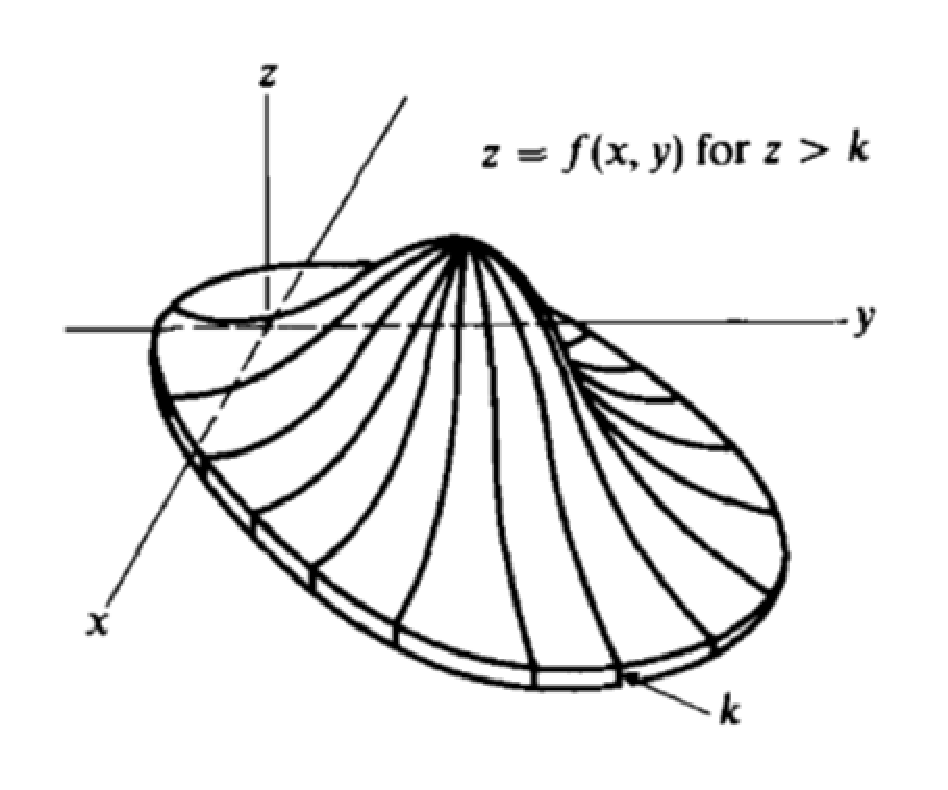
\includegraphics[scale = 0.5]{pictures/bivariate_normal.eps}
\caption{Pravděpodobnostní funkce dvourozměrného normálního rozdělení}
\label{bivariate_normal}
\end{figure}

Příslušná pravděpodobnostní funkce je znározněna na obrázku (\ref{bivariate_normal}). Libovolný řez rovnoběžný s rovinou $xy$ představuje eliptickou křivku, zatímco libovolný řez kolmý na rovninu $xy$ představuje pravděpodobnostní funkci jednorozměrného normálního rozdělení. Pravděpodobnost, že bod $(X,Y)$ leží v regionu $R$ roviny $xy$, je definována jako
\begin{equation*}
P[(X,Y) \in R] = {\int \int}_R f(x,y)dy dx
\end{equation*}

Aby byla pravděpodobnostní funkce dvourozměrného normálního rozdělení pravděpodobnostní funkcí, musí nabývat pouze nezáporných hodnot a musí splňovat podmínku
\begin{equation*}
\int_{-\infty}^{\infty} \int_{-\infty}^{\infty} f(x,y) dy dx = 1
\end{equation*}
Splnění prvního požadavku je patrné ze zběžného pohledu na funkční předpis tohoto pravděpodobnostního rozdělení. Abychom dokázali splnění druhé podmínky, použijeme nejprve substituce
\begin{equation*}
u = \frac{x - E[X]}{\sigma_X}~~~~~v = \frac{y - E[Y]}{\sigma_Y}
\end{equation*}
čímž pravděpodobnostní funkci zjednodušíme do podoby
\begin{equation*}
\int_{-\infty}^{\infty} \int_{-\infty}^{\infty} \frac{1}{2 \pi \sqrt{1 - \rho^2}} e^{-\frac{1}{2(1 - \rho)}(u^2 - 2 \rho u v + v^2)}dv du
\end{equation*}
Doplněním čtverce pro $u$ v exponentu získáváme
\begin{equation*}
\int_{-\infty}^{\infty} \int_{-\infty}^{\infty} \frac{1}{2 \pi \sqrt{1 - \rho^2}}e^{-\frac{1}{2(1 - \rho^2)}[(u - \rho v)^2 + (1 - \rho^2)v^2]}dv du
\end{equation*}
Jestliže dosadíme
\begin{equation*}
w = \frac{u - \rho v}{\sqrt{1 - \rho^2}}~~~~~dw = \frac{du}{\sqrt{1 - \rho^2}}
\end{equation*}
lze výše uvedený integrál rozepsat jako součin dvou jednoduchých integrálů
\begin{equation*}
\int_{-\infty}^{\infty} \frac{1}{\sqrt{2 \pi}}e^{-\frac{w^2}{2}}dw \int_{-\infty}^{\infty} \frac{1}{\sqrt{2 \pi}}e^{-\frac{v^2}{2}}dv
\end{equation*}
které jsou oba rovny jedné.

\subsection{Momentová funkce a momenty}

\begin{theorem}
Sdružená momentová funkce dvourozměrné normální náhodné veličiny $(X,Y)$ je rovna
\begin{equation*}
m(t_1, t_2) = e^{t_1E[X] + t_2E[Y] + \frac{1}{2}(t_1^2 \sigma_X^2 + 2 \rho t_1 t_2 \sigma_X \sigma_Y + t_2^2 \sigma_Y^2)}
\end{equation*}
\end{theorem}

\begin{proof}
Opět dosaďme za $x$ a $y$ veličiny $u$ a $v$, což vede k rovnici
\begin{equation*}
m(t_1, t_2) = e^{t_1E[X] + t_2E[Y]} \int_{-\infty}^{\infty}  \int_{-\infty}^{\infty} e^{t_1 \sigma_X u + t_2 \sigma_Y u} \frac{1}{2 \pi \sqrt{1 - \rho^2}}e^{-\frac{1}{2(1 - \rho^2)}(u^2 - 2 \rho uv + v^2)}dv du
\end{equation*}
Oba exponenty lze sloučit do tvaru
\begin{equation*}
- \frac{1}{2(1 - \rho^2)}\big[u^21 - 2 \rho u v + v^2 - 2(1 - \rho^2)t_1 \sigma_Xu - 2(1 - \rho^2)t_2 \sigma_Y v \big]
\end{equation*}
a doplněním čtverců pro $u$ a $v$ získáme
\begin{gather*}
- \frac{1}{2(1 - \rho^2)}\Big[\big(u - \rho v - (1 - \rho^2)t_1 \sigma_x \big)^2 + (1 - \rho^2)(v - \rho t_1 \sigma_X - t_2 \sigma_Y)^2\\
	-(1 - \rho^2)(t_1^2 \sigma_X^2 + 2 \rho t_1 t_2 \sigma_X \sigma_Y + t_2^2 \sigma_Y^2)\Big]
\end{gather*}
Jestliže použijeme substituce
\begin{equation*}
w = \frac{u - \rho v + (1 - \rho^2)t_1 \sigma_X}{\sqrt{1 - \rho^2}} ~~~~~ z = v - \rho t_1 \sigma_X - t_2 \sigma_Y
\end{equation*}
lze tento výraz dále upravit na
\begin{equation*}
-\frac{1}{2}w^2 - \frac{1}{2}z^2 + \frac{1}{2}(t_1^2 \sigma_X^2 + 2 \rho t_1 t_2 \sigma_X \sigma_Y + t_2^2 \sigma_Y^2)
\end{equation*}
Momentovou funkci pak lze vyjádřit jako
\begin{gather*}
m(t_1, t_2) = e^{t_1 E[X] + t_2 E[X]}e^{\frac{1}{2}(t_1^2 \sigma_X^2 + 2 \rho t_1 t_2 \sigma_X \sigma_Y + t_2^2 \sigma_Y^2)}\int_{-\infty}^{\infty} \int_{-\infty}^{\infty} \frac{1}{2 \pi} e^{-\frac{w^2}{2} - \frac{z^2}{2}}dw dz\\
= e^{t_1 E[X] + t_2 E[Y] + \frac{1}{2}(t_1^2 \sigma_X^2 + 2 \rho t_1 t_2 \sigma_X \sigma_Y + t_2^2 \sigma_Y^2 )}
\end{gather*}
\end{proof}

\begin{theorem}
Jestliže náhodná veličina $(X,Y)$ sleduje dvourozměrné normální rozdělení, pak
\begin{gather*}
\sigma_{X,Y} = \rho \sigma_X \sigma_Y
\end{gather*}
\end{theorem}

\begin{proof}
Sdružený moment $E[X^r Y^s]$ lze získat z  momentové funkce $m(t_1, t_2)$ derivací $r$-krát dle $t_1$ a $s$-krát dle $t_2$ s následným dosazením $t_1 = 0$ a $t_2 = 0$. Kovarianční koeficient $X$ a $Y$ je pak
\begin{gather*}
E[X - E[X]]E[Y - E[Y]] = E[XY - XE[X] - YE[Y] - E[X]E[Y]] = E[XY] - E[X][Y]\\
= \frac{\partial^2}{\partial t_1 \partial t_2}m(t_1, t_2)\Big|_{t_1 = t_2 = 0} - E[X]E[Y] = \rho \sigma_X \sigma_Y
\end{gather*}
\end{proof}

\begin{theorem}
Jestliže má náhodná veličina $(X,Y)$ dvourozměrné normální rozdělení, pak jsou $X$ a $Y$ nezávislé tehdy a jen tehdy, jsou-li $X$ a $Y$ nekorelované.
\end{theorem}

\begin{proof}
Náhodné veličiny jsou nekorelované tehdy a jen tehdy, je-li $\sigma_{X,Y} = 0$ nebo ekvivalentně je-li $\rho_{X,Y} = 0$. Z definice dvourozměrného normálního rozdělení je zřejmé, že je-li $\rho_{X,Y} = 0$, pak se pravděpodobnostní funkce $f_{X,Y}$ stane součinem dvou jednorozměrných normálních rozdělení. Proto $\rho_{X,Y}$ implikuje, že $X$ a $Y$ jsou nezávislé. Víme, že nezávislost náhodných veličin $X$ a $Y$ implikuje jejich nekorelovanost.
\end{proof}

\section{Marginální a podmníněná pravděpodobnostní funkce}

\begin{theorem}
Jestliže $(X,Y)$ sleduje dvourozměrné náhodné rozdělení, pak marginální rozdělení $X$ a $Y$ jsou jednorozměrná normální rozdělení. To znamená, že $X$ je normálně rozdělené se střední hodnotou $E[X]$ a rozptylem $\sigma_X^2$ a $Y$ je normálně rozdělené se střední hodnotou $E[X]$ a rozptylem $\sigma_Y^2$.
\end{theorem}

\begin{proof}
Marginální rozdělení náhodné veličiny $X$ je z definice
\begin{equation*}
f_X(x) = \int_{-\infty}^{\infty} f(x,y)dy
\end{equation*}
S použím substituce $v = \frac{y - E[Y]}{\sigma_Y}$ a doplněním čtverců pro $v$ získáme
\begin{equation*}
f_X(x) = \int_{-\infty}^{\infty} \frac{1}{2 \pi \sigma_X \sqrt{1 - \rho^2}} e^{-\frac{1}{2} \big(\frac{x - E[X]}{\sigma_X} \big)^2 - \frac{1}{2(1 - \rho)^2} \big(v - \rho \frac{x - E[X]}{\sigma_X} \big)^2}dv
\end{equation*}
Následnými substitucemi
\begin{equation*}
w = \frac{v - \rho(x - E[X])/ \sigma_X}{\sqrt{1 - \rho^2}} ~~~~~ dw \frac{1}{\sqrt{1 - \rho^2}}dv
\end{equation*}
lze dokázat
\begin{equation*}
f_X(x) = \frac{1}{\sqrt{2 \pi \sigma_X^2}} e^{-\frac{1}{2}\big(\frac{y - E[Y]}{\sigma_Y} \big)^2}
\end{equation*}
Analogicky lze důkaz provést také pro $f_Y(y)$.
\end{proof}
\begin{theorem}
Jestliže $(X,Y)$ sleduje dvourozměrné normální rozdělení, pak podmíněná pravděpodobnostní funkce náhodné veličiny $X$ pro $Y = y$ sleduje normální rozdělení se střední hodnotou $E[X] + \rho \frac{\sigma_X}{\sigma_Y}(y - E[Y])$ a rozptylem $\sigma_X^2(1 - \rho^2)$. Podobně podmíněná pravděpodobnostní funkce náhodné veličiny $Y$ pro $X = x$ sleduje normální rozdělení se střední hodnotou $E[Y] + \rho \frac{\sigma_Y}{\sigma_X}(x - E[X])$ a rozptylem $\sigma_Y^2(1 - \rho^2)$.
\end{theorem}

\begin{proof}
Podmíněné pravděpodobnostní funkce lze odvodit s pomocí sdružené a marginální pravděpodobnostní funkce.
\begin{equation*}
f_{X|Y}(x|y) = \frac{f(x,y)}{f_Y(y)}
\end{equation*}
Dosazením a následnými úpravami získáme
\begin{equation*}
f_{X|Y}(x|y) = \frac{1}{\sqrt{2 \pi} \sigma_X \sqrt{1 - \rho^2}}e^{-\frac{1}{2 \sigma_X^2(1 - \rho^2)}\big[x - E[X] - \frac{\rho \sigma_X}{\sigma_Y}(y - E[Y]) \big]^2}
\end{equation*}
což je jednorozměrné normální rozdělení se střední hodnotou $E[X] + \rho \frac{\sigma_X}{\sigma_Y}(y - E[Y])$ a rozptylem $\sigma_X^2(1 - \rho^2)$. Analogicky lze odvodit také $f_{Y|X}(y|x)$.
\end{proof}

Již dříve jsme zmínili, že v případě podmíněného rozdělení nazýváme střední hodnotau náhodné veličiny regresní křivkou. Ve výše uvedeném případě je regrese $X$ pro $Y = y$ rovna $E[X] + \rho \frac{\sigma_X}{\sigma_Y}(y - E[Y])$, což je lineární funkce veličiny $y$.

\begin{figure}[htp]
\centering
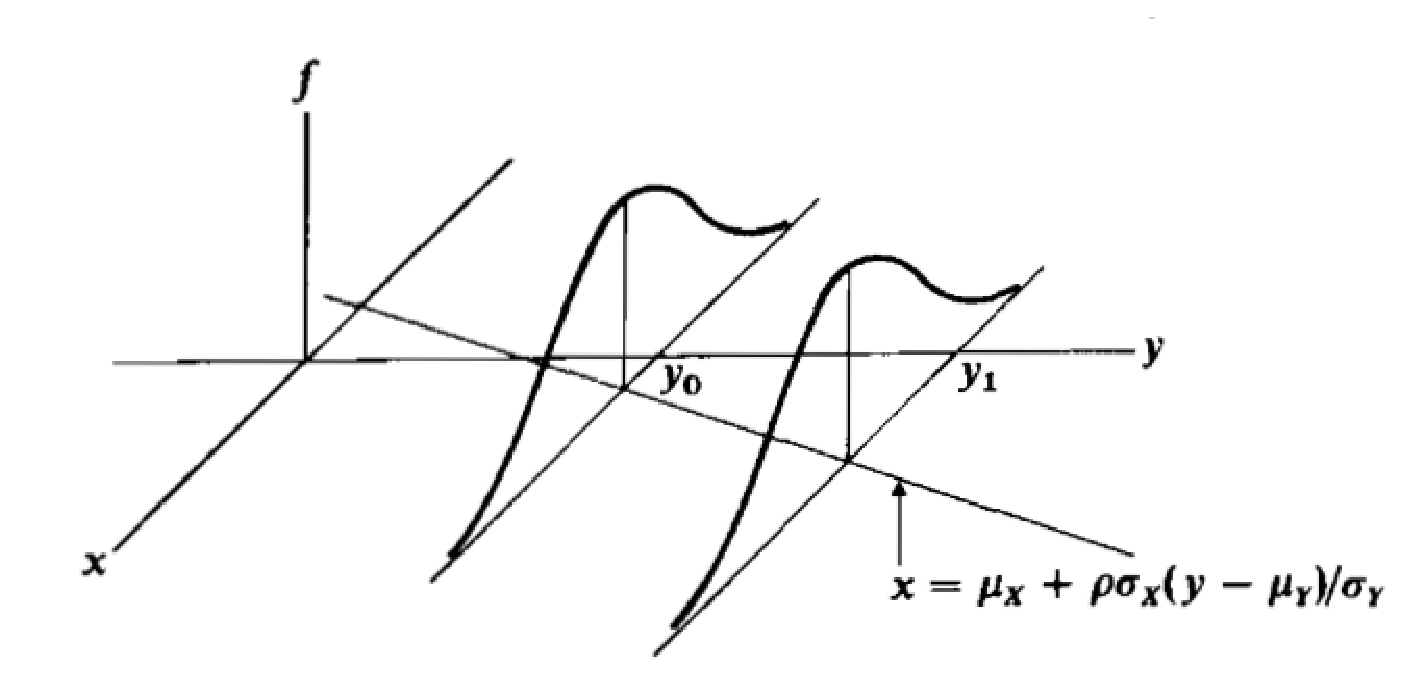
\includegraphics[scale = 0.5]{pictures/bivariate_normal_regression.eps}
\caption{Regresní křivka pro podmíněné dvourozměrné normální rozdělení}
\label{bivariate_normal_regression}
\end{figure}  
 


\chapter{Distribuce funkcí náhodných veličin}

\section{Střední hodnota a rozptyl funkcí náhodných veličin}

\subsection{Dvojí pojetí}

Uvažujme funkci $g(\cdot, ..., \cdot)$ a náhodné veličiny $X_1, ..., X_n$. Definujme náhodnou veličinu $Y = g(X_1, ..., X_n)$. Střední hodnotu náhodné veličiny $Y$ lze vypočíst dvěma způsoby a to buď jako
\begin{equation*}
E[Y] = \int_{-\infty}^{\infty} y f_Y(y)dy
\end{equation*}
nebo jako
\begin{equation*}
E[Y] = E[g(X_1, ..., X_n)] = \int_{-\infty}^{\infty} \cdots \int_{-\infty}^{\infty} g(x_1, ..., x_2)f_{X_1, ..., X_2}(x_1, ..., x_n)dx_1 \cdots dx_n
\end{equation*}
Na první pohled by se mohlo zdát, že je výhodnější řešit $E[Y]$ prvním způsobem, protože se tak vyhneme vícenásobnému intergrálu. Situaci však může značně zkomplikovat pravděpodobnostní funkce $f_Y(\cdot)$, jejíž znalost je nezbytným předpokladem pro zahájení výpočtu.

\begin{example}
Nechť náhodná veličina $X$ sleduje normované normální rozdělení a nechť $g(x) = x^2$. Střední hodnotu náhodné veličiny $Y = g(X)$ tak lze vypočíst jako
\begin{equation*}
E[Y] = \int_0^{\infty} y \frac{1}{\Gamma(1/2)}\Big(\frac{1}{2} \Big)^{\frac{1}{2}}y^{-\frac{1}{2}}e^{-\frac{1}{2}y}dy = 1
\end{equation*}
kde jsme využili skutečnost, že náhodná veličina $Y$ sleduje gamma rozdělení s parametry $r = \frac{1}{2}$ a $\lambda = \frac{1}{2}$. Alternativně lze $E[Y]$ vypočíst ze vztahu
\begin{equation*}
E[X^2] = \int_{-\infty}^{\infty}x^2 \frac{1}{\sqrt{2 \pi}}e^{-\frac{1}{2}x^2}dx = 1
\end{equation*}
\end{example}

\subsection{Součet náhodných veličin}

\begin{theorem}
Pro náhodné veličiny $X_1, ..., X_n$ platí
\begin{equation*}
E\Big[\sum_1^n X_i \Big] = \sum_1^n E[X_i]
\end{equation*}
a
\begin{equation*}
D\Big[\sum_1^n X_i \Big] = \sum_1^n D[X_i] + 2 \sum \sum_{i < j} \sigma_{X_i, X_j}
\end{equation*}
\end{theorem}

\begin{proof}
Dokažme tvrzení o rozptylu součtu náhodoných veličin.
\begin{gather*}
D\Big[\sum_1^n X_i \Big] = E \Big[\Big(\sum_1^n X_i - E\Big[\sum_1^n X_i\Big] \Big)^2 \Big] = E\Big[\Big(\sum_1^n(X_i - E[_i]) \Big)^2 \Big]\\
= E \Big[\sum_{i = 1}^n \sum_{j = 1}^n (X_i - E[X_i])(X_j - E[X_j]) \Big] = \sum_{i = 1}^n \sum_{j = 1}^nE[(X_ - E[X_i])(X_j - E[X_j])]\\
= \sum_{i = 1}^n D[X_i] + 2 \sum \sum_{i < j} \sigma_{X_i, X_j}
\end{gather*}
\end{proof}

\begin{corollary}
Jestliže jsou $X_1, ..., X_n$ nekorelované náhodné veličiny, pak
\begin{equation*}
D\Big[\sum_1^n X_i  \Big] = \sum_1^n D[X_i]
\end{equation*}
\end{corollary}

\chapter{Výběry a jejich rozdělení}

\section{Výběr a populace}

\subsection{Definice základních pojmů}

\begin{definition}[Cílová populace]
Soubor všech prvků, které jsou předmětem našeho zájmu, nazýváme cílovou populací.
\end{definition}

\begin{example}
V astronomii můžeme být cílovou populací soubor všech hvězd ve vesmíru a předmětem zájmu jejich hmotnost. V letectví mohou cílovou skupinu představovat všechny vyrobené letouny daného typu, kde zkoumáme životnost jejich draku.
\end{example}

V praxi bývá velmi často nemožné nebo nežádoucí zjišťovat danou vlastnost na celé cílové populaci\footnote{Hvězd ve vesmíru je příliš mnoho na to, abychom je mohli všechny jednotlivě zkoumat. Testování odolnosti draku všech letounů by vedlo k jejich zničení, a proto postrádá smysl.}. Řešením je tak vybrat část populace a tu následně podrobit zkoumání - zjištění pak zobecníme na celou populaci.

Jestliže lze na každý prvek cílové populace nahlížet jako na náhodnou veličinu s danou pravděpodobnostní funkcí\footnote{Na hmotnost hvězdy a na životnost draku letadla lze zcela jistě pohlížet jako na náhodnou veličinu.}, pak lze pro tuto populaci definovat náhodný výběr.

\begin{definition}[Náhodný výběr]
Nechť mají náhodné veličiny $X_1, ..., X_n$ sdruženou pravděpodobnostní funkci, pro kterou platí
\begin{equation*}
f_{X_1, ..., X_n}(x_1, ..., x_n) = f(x_1) \cdots f(x_n)
\end{equation*}
kde $f(\cdot)$ představuje pravděpodobnostní funkci, která je shodná pro všechna $X_i$. Pak definujeme $X_1, ..., X_n$ jako náhodný výběr velikosti $n$ z populace s pravděpodobnostní funkcí $f(\cdot)$.
\end{definition}

Náhodná veličina $X_i$ reprezentuje hodnotu $i$-tého prvku výběru. Po té, co je výběr zanalyzován, nabývá náhodná veličina $X_i$ konkrétní hodnoty $x_i$. Proto se někdy pod pojmem náhodný výběr rozumí $x_1, ..., x_n$ namísto $X_1, ..., X_n$.

Velmi často není možné pořídit náhodný výběr z cílové populace. V těchto případech pak cílovou populaci nahrazujeme tzv. výběrovou populací.

\begin{definition}[Výběrová populace]
Nechť $X_1, ..., X_n$ je náhodný výběr z populace s pravděpodobnostní funkcí $f(\cdot)$. Tuto populaci pak nazýváme výběrovou populací.
\end{definition}

Závěry na základě náhodného výběru lze vztáhnout pouze na výběrovou populaci, nikoliv na cílovou populaci. Jedinou vyjímkou je situace, kdy je cílová populace zároveň výběrovou populací.

\begin{example}
Uvažujme marketingovou studii, jejímž cílem je zkoumat nákupní zvyky domácností dané země. Pokud budeme náhodný vzorek domácností vybírat z určitého regionu, pak tento region bude představovat naši výběrovou populaci. Naší cílovou populací však budou dománosti celé země. Je také zřejmé, že nákupní zvyklosti domácností se mohou mezi jednotlivými regiony lišit, a proto zobecnění z jednoho regionu na celou zemi může být problematické.
\end{example}

V následujícím textu budeme někdy používat označení ``populace $f(\cdot)$'', čímž budeme mít na mysli populaci, jejíž jednotlivé prvky mají pravděpodobnostní rozdělení $f(\cdot)$. Pokud budeme používat slovo populace bez přívlastku, budeme tím mít na mysli vždy výběrovou populaci.

\subsection{Rozdělení výběru}

\begin{definition}[Rozdělení výběru]
Nechť $X_1, ..., X_n$ označují náhodný výběr velikosti $n$. Pak rozdělení výběru $X_1, ..., X_n$ je dáno sdruženým rozdělením náhodných veličin $X_1, ..., X_n$.
\end{definition}

\begin{definition}
Jestliže $X_1, ..., X_n$ představují náhodný výběr z populace $f(\cdot)$, pak pravděpodobnostní rozdělení tohoto výběru je dáno sdruženou pravděpodobnostní funkcí
\begin{equation*}
f_{X_1, ..., X_n}(x_1, ..., x_n)(x_1, ..., x_n) = f(x_1) \cdots f(x_n)
\end{equation*}
\end{definition}

\begin{example}
Uvažujme populaci, jejíž prvky sledují Bernoulliho rozdělení. Sdružená pravděpodobnostní funkce dvou prvkového náhodného výběru je tedy
\begin{equation*}
f_{X_1, X_2}(x_1, x_2) = f(x_1)f(x_2) = p^{x_1 + x_2}q^{2 - x_1 - x_2}I_{(0, 1)}(x_1)I_{(0, 1)}(x_2)
\end{equation*}
\end{example}

Pravděpodobnostní funkce $f_{X_1, X_2}(x_1, x_2)$ z výše uvedeného příkladu definuje rozdělení uspořádaného výběru. Záleží tedy nejen na typu a počtu realizací, ale také na jejich uspořádání.

Dále je zřejmé, že naše definice náhodného výběru automaticky zavrhuje výběr bez vracení z konečné populace, protože jednotlivé ``tahy'' nejsou vzájemně nezávislé.

\subsection{Statistiky a výběrové momenty}

\begin{definition}[Statistika]
Statistika je funkcí pozorovatelných náhodných veličin, a je tak sama o sobě pozorovatelnou náhodnou veličinou, která neobsahuje žádné neznámé parametry. 
\end{definition}

\begin{example}
Jestliže $X_1, ..., X_n$ představuje náhodný výběr z populace $f(\cdot, \theta)$, pak, za předpokladu, že $X_1, ..., X_n$ jsou pozorovatelné, jsou
\begin{equation*}
\overline{X}_n = \frac{1}{n} \sum_{i = 1}^n X_i
\end{equation*}
a
\begin{equation*}
\frac{1}{2}(\min(X_1, ..., X_n) + \max(X_1, ..., X_n))
\end{equation*}
statistikami. Pokud $f(x, \theta) = \phi_{\theta, 1}(x)$, kde $\theta$ je neznámý parametr, pak $\overline{X}_n - \theta$ není statistikou, právě proto, že závisí na neznámé $\theta$. 
\end{example}

V následující definici představíme jedny z  nejdůležitějších statistik, tzv. výběrové momenty.

\begin{definition}[Výběrové momenty]
Nechť $X_1, ..., X_n$ představuje náhodný výběr z populace $f(\cdot)$. Pak je $r$-tý obecný výběrový moment definován jako
\begin{equation*}
M'_r = \frac{1}{n} \sum_{i = 1}^n X_i^r
\end{equation*}
Jestliže $r = 1$, pak získáme výběrový moment obvykle označovaný jako $\overline{X}$ popř. jako $\overline{X}_n$.
\begin{equation*}
\overline{X}_n = \frac{1}{n} \sum_{i = 1}^n X_i
\end{equation*}
Podobně je $r$-tý centrální výběrový moment definován jako
\begin{equation*}
M_r = \frac{1}{n} \sum_{i = 1}^n \left(X_i - \overline{X}_n \right)^r
\end{equation*}
\end{definition}

\begin{theorem}
Nechť $X_1, ..., X_n$ představují náhodný výběr z populace $f(\cdot)$. Očekávaná hodnota $r$-tého výběrového momentu $M'_r$ je rovna $r$-tému momentu populace $\mu'_r$ za předpokladu existence $\mu'_r$. 
\begin{equation*}
E[M'_r] = \mu'_r
\end{equation*}
Dále také platí
\begin{equation*}
D[M'_r] = \frac{1}{n}\left(E[X^{2r}] - E[X^r]^2 \right) = \frac{1}{n} [\mu'_{2r} - (\mu'_r)^2]
\end{equation*}
za předpokladu existence $\mu'_{2r}$.
\end{theorem}

\begin{proof}
\begin{gather*}
E[M'_r] = E \left[\frac{1}{n} \sum_{i = 1}^n X_i^r \right] = \frac{1}{n} E \left[\sum_{i = 1}^n X_i^r \right] = \frac{1}{n} \sum_{i = 1}^n E[X_i^r] = \frac{1}{n} \sum_{i = 1}^n \mu'_r = \mu'_r
\end{gather*}
\begin{gather*}
D[M'_r] = D\left[\frac{1}{n} \sum_{i = 1}^n X_i^r \right] = \left(\frac{1}{n} \right)^2 D \left[ \sum_{i = 1}^n X_i^r \right] = \left(\frac{1}{n} \right)^2 \sum_{i = 1}^n \left(E[X_i^{2r}] - E[X_i^r]^2 \right)\\
= \frac{1}{n} \left(E[X^2r] - E[X^r]^2 \right) = \frac{1}{n}\left(\mu'_{2r} - (\mu'_r)^2 \right)
\end{gather*}
\end{proof}

\begin{corollary}
Nechť $X_1, ..., X_n$ představuje náhodný výběr z populace $f(\cdot)$ a $\overline{X}_n = \frac{1}{n} \sum_{i = 1}^n X_i$ představuje výběrovou střední hodnotu. Pak platí
\begin{gather*}
E[\overline{X}_n] = \mu\\
D[\overline{X}_n] = \frac{1}{n} \sigma^2
\end{gather*}
kde $\mu$ a $\sigma^2$ jsou střední hodnota a rozptyl pravděpodobnostního rozdělení $f(\cdot)$.
\end{corollary}

\begin{definition}[Výběrový rozptyl]
Nechť $X_1, ..., X_n$ představují náhodný výběr z populace $f(\cdot)$. Výběrový rozptyl je pak definován jako
\begin{equation*}
S_n^2 = \frac{1}{n - 1} \sum_{i = 1}^n (X_i - \overline{X})^2
\end{equation*}
pro $n > 1$.
\end{definition}

Výběrový rozptyl je definován jako $S_n^2 = \frac{1}{n - 1} \sum_{i = 1}^n (X_i - \overline{X})^2$ namísto druhého výběrového momentu $M_2 = \frac{1}{n} \sum_{i = 1}^n (X_i - \overline{X})^2$, protože střední hodnota $S_n^2$ je rovna rozptylu populace.

\begin{corollary}
\begin{equation*}
S_n^2 = \frac{1}{2n(n-1)} \sum_{i = 1}^n \sum_{j = 1}^n (X_i - X_j)^2
\end{equation*}
\end{corollary}

\begin{proof}
\begin{gather*}
\frac{1}{2n(n - 1)} \sum_{i = 1}^n \sum_{j = 1}^n (X_i - X_j)^2 = \frac{1}{2n(n - 1)}\sum_{i = 1}^n \left(nX_i^2 - 2 X_i \sum_{j = 1}^n X_j + \sum_{j = 1}^n X_j^2 \right)\\
= \frac{1}{2n(n - 1)} \sum_{i = 1}^n \left(nX_i^2 - 2n \overline{X}X_i + n \overline{X^2} \right) = \frac{1}{2(n-1)}\left(n \overline{X^2} - 2 \overline{X}^2 + n \overline{X^2} \right)\\
= \frac{1}{n - 1}(n\overline{X^2} - \overline{X}^2) = \frac{1}{n - 1}nD[X] = \frac{1}{n - 1}\sum_{i = 1}^n (X_i - \overline{X})^2
\end{gather*}
\end{proof}

\begin{theorem}
Nechť $X_1, ..., X_n$ představuje náhodný výběr z populace $f(\cdot)$ a nechť $S_n^2 = \frac{1}{n - 1} \sum_{i = 1}^n (X_i - \overline{X})^2$. Pak platí
\begin{gather*}
E[S_n^2] = \sigma^2\\
D[S_n^2] = \frac{1}{n}\left(\mu_4 - \frac{n - 3}{n - 1}\sigma^4 \right)
\end{gather*}
pro $n > 1$.
\end{theorem}

\begin{proof}
Nejprve dokažme tvrzení o střední hodnotě výběrového rozptylu. Připomeňme, že platí $\sigma^2 = E[(X - \mu)^2]$ a $\mu_r = E[(X - \mu)^r]$. Jádro důkazu spočívá v identitě
\begin{equation*}
\sum_{i = 1}^n (X_i - \mu)^2 = \sum_{i = 1}^n (X_i - \overline{X})^2 + n (\overline{X} - \mu)^2
\end{equation*}
Platnost této identity lze dokázat následujícím způsobem.
\begin{gather*}
\sum(X_i - \mu)^2 = \sum(X_i - \overline{X} + \overline{X} - \mu)^2 = \sum [(X_i - \overline{X}) + (\overline{X} - \mu)]^2]\\
= \sum[(X_i - \overline{X})^2 + 2(X_i - \overline{X})(\overline{X} - \mu) + (\overline{X} - \mu)^2]\\
= \sum(X_i - \overline{X})^2 + 2(\overline{X} - \mu)\sum(X_i - \overline{X}) + n (\overline{X} - \mu)^2
= \sum(X_i - \overline{X})^2 + n(\overline{X} - \mu)^2
\end{gather*}
S využitím této identity pak lze odvodit
\begin{gather*}
E[S_n^2] = E \left[\frac{1}{n - 1} \sum (X_i - \overline{X})^2 \right] = \frac{1}{n - 1} E \left[\sum_{i = 1}^n (X_i - \mu)^2 - n(\overline{X} - \mu)^2 \right]\\
\frac{1}{n - 1} \Big\{\sum_{i = 1}^n E[(X_i - \mu)^2] - n E[(\overline{X} - \mu)^2] \Big\} = \frac{1}{n - 1}\Big\{\sum_{i = 1}^n \sigma^2 - n D[\overline{X}] \Big\}\\
= \frac{1}{n - 1}\left(n \sigma^2 - n \frac{\sigma^2}{n} \right) = \sigma^2
\end{gather*}

Důkaz rozptylu $S_n^2$ lze provést s využitím výše odvozené identity a vztahu
\begin{equation*}
\overline{X} - \mu = \frac{1}{n} \sum X_i - \frac{1}{n} n \mu = \frac{1}{n} \sum X_i - \frac{1}{n} \sum \mu = \frac{1}{n} \sum (X_i - \mu)
\end{equation*}
Nicméně odvození je poměrně zdlouhavé, a proto jej vynecháme.
\end{proof}

\section{Výběrová střední hodnota}

\subsection{Střední hodnota a rozptyl}

\begin{theorem}
Nechť $X_1, ..., X_n$ představuje náhodný výběr z populace $f(\cdot)$ se střední hodnotou $\mu$ a konečným rozptylem $\sigma^2$. Definujme $\overline{X} = \frac{1}{n} \sum_{i = 1}^n X_i$. Pak platí
\begin{equation*}
E[\overline{X}] = \mu_{\overline{x}} = \mu ~~~ D[\overline{X}] = \sigma_{\overline{X}^2} = \frac{1}{n} \sigma^2
\end{equation*}
\end{theorem}
Tento teorém je v podstatě pouze reformulací tvrzení (6.1).

Výběrová střední hodnota $\overline{X}$ má charakter náhodné veličiny. Pokud bychom ji použili jako odhad pro $\mu$, pak platí, že její střední hodnota odpovídá hledané střední hodnotě populace $\mu$ a že její rozptyl klesá s rostoucí velikostí náhodného výběru. Tímto se dostáváme k zákonu velkých čísel.

\subsection{Zákon velkých čísel}

Označme střední hodnotu náhodné veličiny $X$ s pravděpodobnostní funkcí $f(\cdot)$ jako $\mu$. Předpokládejme, že předmětem našeho zájmu je odhad $\mu$.

Na $\mu$ lze nahlížet jako na průměr nekonečného počtu hodnot náhodné veličiny $X$. Je zřejmé, že reálném životě nejsme schopni průměrovat nekonečný počet hodnot, a proto musíme informace o $\mu$ získat na základě náhodného výběru z populace $f(\cdot)$ velikosti $n$. To nám umožňuje tzv. slabý zákon velkých čísel.

\begin{theorem}[Slabý zákon velkých čísel]
Nechť $f(\cdot)$ představuje pravděpodobnostní funkci se střední hodnotou $\mu$ a rozptylem $\sigma^2$. Dále nechť $\overline{X}_n$ představuje střední hodnotu náhodného výběru velikosti $n$ z populace $f(\cdot)$. Uvažujme dvě čísla $\epsilon > 0$ a $0 < \delta < 1$. Jestliže $n$ je přirozené číslo takové, že $n > \frac{\sigma^2}{\epsilon^2} \delta$, pak
\begin{equation*}
P[-\epsilon < \overline{X}_n - \mu < \epsilon] \ge 1 - \delta
\end{equation*}  
\end{theorem}  

\begin{proof}
Dle Chebyshevovy nerovnosti platí
\begin{equation*}
P[g(X) \ge k] \le \frac{E[g(X)]}{k}
\end{equation*}
pro každé $k > 0$, libovolnou náhodnou veličinu $X$ a nezápornou funkci $g(\cdot)$. Tato nerovnost je ekvivalentní s
\begin{equation*}
P[g(X) < k] \ge 1 - \frac{E[g(X)]}{k}
\end{equation*}
Nechť $g(X) = (\overline{X}_n - \mu)^2$ a $k = \epsilon^2$. Pak
\begin{gather*}
P[-\epsilon < \overline{X}_n - \mu < \epsilon] = P[|\overline{X}_n - \mu| < \epsilon]\\
= P[|\overline{X}_n - \mu|^2 < \epsilon^2] \ge 1 - \frac{E[(\overline{X}_n - \mu)^2]}{\epsilon^2}\\
= 1 - \frac{\frac{1}{n}\sigma^2}{\epsilon^2} \ge 1 - \delta
\end{gather*}
pro $\delta > \frac{\sigma^2}{n \epsilon^2}$ popř. $n > \frac{\sigma^2}{\epsilon^2} \delta$.
\end{proof}

\begin{example}
Uvažujme pravděpodobnostní rozdělení s neznámou střední hodnotou a rozptylem 1. Jak velký musí být náhodný výběr, aby se jeho střední hodnota $\overline{X}_n$ nacházela ve vzdálenosti 0.5 od střední hodnoty populace s pravděpodobnostní alespoň 0.95?

Dosaďme $\sigma^2 = 1, \epsilon = 0.5$ a $\delta = 0.05$. Minimální velikost $n$ náhodného výběru je dána vztahem
\begin{equation*}
n > \frac{\sigma^2}{\delta \epsilon} = \frac{1}{0.05 \cdot (0.5)^2} = 80
\end{equation*} 
\end{example}

\subsection{Centrální limitní věta}

S centrální limitní větou jsme se již seznámili v předchozí kapitole. Nyní se k ní opět vrátíme a doplníme ji o důkaz.

\begin{theorem}[Centrální limitní věta]
Nechť $f(\cdot)$ představuje pravděpodobnostní funkci se střední hodnotou $\mu$ a konečným rozptylem $\sigma^2$. Dále nechť $\overline{X}_n$ představuje střední hodnotu náhodného výběru velikosti $n$ z populace $f(\cdot)$. Definujme náhodnou veličinu
\begin{equation*}
Z_n = \frac{\overline{X}_n - E[\overline{X}_n]}{\sqrt{D[\overline{X}_n]}} = \frac{\overline{X}_n - \mu}{\frac{\sigma}{\sqrt{n}}}
\end{equation*}
Pravděpodobnostní rozdělení náhodné veličiny $Z_n$ se limitně blíží normovanému normálnímu rozdělení s tím, jak se $n$ blíží nekonečnu.
\end{theorem}
Nejpozoruhodnější skutečností na centrální limitní větě je, že platí pro všechny pravděpodobnostní funkce $f(\cdot)$. Centrální limitní věta implikuje, že pravděpodobnostní funkce výběrové střední hodnoty $\overline{X}_n$ se asymptoticky blíží normálnímu rozdělení se střední hodnotou $\mu$ a rozptylem $\frac{\sigma^2}{n}$ bez ohledu na výchozí pravděpodobnosntí funkci $f(\cdot)$.

\begin{proof}
Centrální limitní větu nebudeme dokazovat v její obecné formě. Zaměříme se na situaci, kdy $f(\cdot)$ má momentovou funkci. Připomeňme, že momentová funkce normovaného normálního rozdělení je $m(t) = e^{\frac{1}{2}t^2}$. Pro momentovou funkci $m_{Z_n}(t)$ náhodné veličiny $Z_n$ se pak pokusíme dokázat, že se asymptoticky blíží k $m(t)$. 

Momentová funkce $m_{Z_n}(t)$ je definována jako
\begin{gather*}
m_{Z_n}(t) = E[e^{tZ_n}] = E\left[e^{t\frac{\overline{X} - \mu}{\sigma / \sqrt{n}}} \right] = E\left[e^{\frac{t}{n}\sum \frac{X_i - \mu}{\sigma / \sqrt{n}}} \right]\\
= E\left[\prod_{i = 1}^n e^{\frac{t}{n} \frac{X_i - \mu}{\sigma / \sqrt{n}}} \right] = \prod_{i = 1}^n E \left[e^{\frac{t}{\sqrt{n}}\frac{X_i - \mu}{\sigma}} \right]
\end{gather*}
kde jsme v posledním kroku využili nezávislosti náhodných veličin $X_1, ..., X_n$. Definujme $Y_i = \frac{X_i - \mu}{\sigma}$. Momentová funkce náhodné veličiny $Y_i$ je nezávislá na $i$, protože všechna $Y_i$ mají shodné pravděpodobnostní rozdělení. Proto namísto $m_{Y_i}(t)$ budeme používat značení $m_Y(t)$. Platí
\begin{gather*}
\prod_{i = 1}^n E \left[e^{\frac{t}{\sqrt{n}} \frac{X_i - \mu}{\sigma}} \right] = \prod_{i = 1}^n e^{\frac{t}{\sqrt{n}} Y_i}\\
= \prod_{i = 1}^n m_Y\left(\frac{t}{\sqrt{n}}\right) = \left[m_Y\left(\frac{t}{\sqrt{n}}\right)\right]^n
\end{gather*}
a proto
\begin{equation*}
m_{Z_n(t)} = \left[m_Y \left(\frac{t}{\sqrt{n}}\right)\right]^n
\end{equation*}
$r$-tou derivací $m_Y(t/\sqrt{n})$ v bodě $t = 0$ získáme $r$-tý moment okolo střední hodnoty pro pravděpodobnostní funkci $f(\cdot)$ vydělený členem $(\sigma \sqrt{n})^r$. S pomocí Taylorova rozvoje tak lze $m_Y(t/\sqrt{n})$ vyjádřit jako
\begin{equation*}
m_Y\left(\frac{t}{\sqrt{n}}\right) = 1 + \frac{\mu_1}{\sigma}\frac{t}{\sqrt{n}}+\frac{1}{2!}\frac{\mu_2}{\sigma^2} \left(\frac{t}{\sqrt{n}}\right)^2 + \frac{1}{3!} \frac{\mu_3}{\sigma^3} \left(\frac{t}{\sqrt{n}}\right)^3 + \cdots
\end{equation*}
a protože $\mu_1 = 0$ a $\mu_2 = \sigma^2$, lze tento výraz dále upravit na
\begin{equation*}
m_Y\left(\frac{t}{\sqrt{n}}\right) = 1 + \frac{1}{n}\left(\frac{1}{2}t^2 + \frac{1}{3! \sqrt{n}}\frac{\mu_3}{\sigma^3} t^3 + \frac{1}{4!n}\frac{\mu_4}{\sigma^4}t^4 + \cdots \right)
\end{equation*}
Protože $\lim_{n \rightarrow \infty}\left(1 + \frac{u}{n} \right)^n = e^{\frac{1}{2}t^2}$, kde
\begin{equation*}
u = \frac{1}{2}t^2 + \frac{1}{3! \sqrt{n}}\frac{\mu_3}{\sigma^3} t^3 + \frac{1}{4!n}\frac{\mu_4}{\sigma^4}t^4 + \cdots
\end{equation*}
představuje výraz v závorkách ve výše uvedené rovnici. Tím se dostáváme k $\lim_{n \rightarrow \infty} m_{Z_n}(t) = e^{\frac{1}{2}t^2}$. Proto má $Z_n$ v limitě stejnou momentovou funkci jako normalizované normální rozdělení. Připomeňme, že pokud mají dvě náhodné veličiny shodnou momentovou funkci, pak sledují shodné pravděpodobnostní rozdělení.
\end{proof}

Je zřejmé, že míra aproximace záleží na velikosti náhodného výběru a konkrétní pravděpodobnostní funkci $f(\cdot)$. Situace pro $f(x) = e^{-x}I_{(0, \infty)}(x)$ pro $n = 1, 3, 10$ je ilustrována obrázkem (\ref{asymptotic-normal}), kde souvislá čára představuje skutečné rozdělení a přerušovaná čára pak aproximaci normálním rozdělením.

\begin{figure}[htp]
\centering
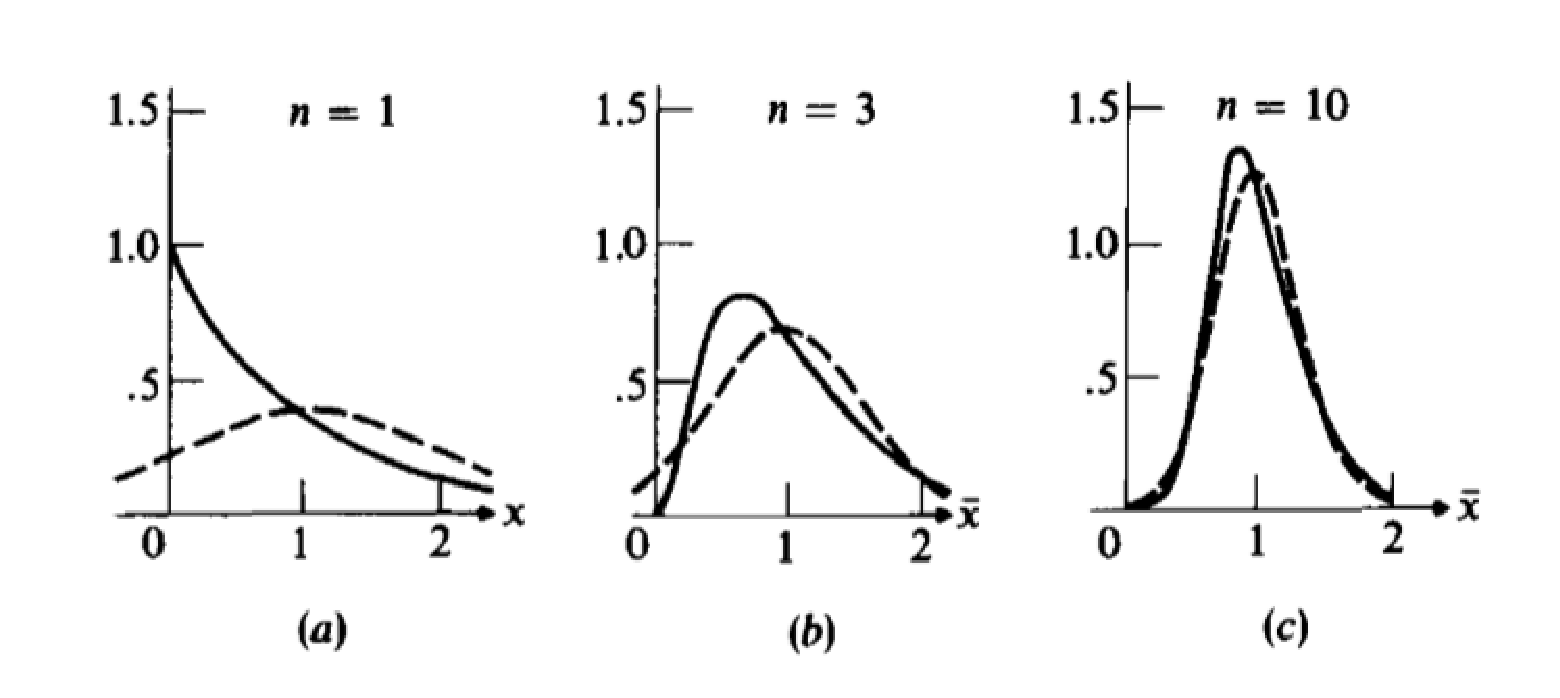
\includegraphics[scale = 0.5]{pictures/asymptotic_normal.eps}
\caption{Konvergence k normálnímu rozdělení}
\label{asymptotic-normal}
\end{figure}

Jak je z obrázku (\ref{asymptotic-normal}) patrné, aproximace se poměrně rychle zlepšuje s rostoucí velikostí náhodného výběru. Obrázek se zaměřuje na konvergenci v okolí střední hodnoty $\mu$. Co z něj však patrné není, je konvergence v okolí chvostů, kde je míra konvergence výrazně pomalejší.

Následující kapitoly se zaměřují na pravděpodobnostní rozdělení střední hodnoty výběru pro konkrétní pravděpodobnostní funkci $f(\cdot)$.

\subsection{Bernoulliho rozdělení}

Jestliže $X_1, ..., X_n$ představují náhodný výběr z Bernoulliho rozdělení, lze nalézt přesnou formu pravděpodobnostního rozdělení náhodné veličiny $\overline{X}_n$. Pravděpodobnostní funkce, ze které provádíme náhodný výběr, má formu
\begin{equation*}
f(x) = p^x(1 - p)^{1 - x}I_{(0, 1)}(x)
\end{equation*}
Z příkladu (5.7) víme, že $\sum_{i = 1}^n X_i$ sleduje binomické rozdělení.
\begin{equation*}
P \left[\sum_{i = 1}^n X_i = k \right] = \binom{n}{k}p^k q^{n - k}I_{\{0, 1, ..., n\}}(k)
\end{equation*}
Proto je pravděpodobnostní rozdělení $\overline{X}_n$ dáno vztahem
\begin{equation*}
P \left[\overline{X}_n = \frac{k}{n} \right] = \binom{n}{k}p^k q^{n - k}~~~\textit{pro}~ k = 0, 1, ..., n 
\end{equation*}
Proto náhodná veličina $\overline{X}_n$ nabývá v případě Bernoulliho rozdělení hodnot $0, 1/n, ..., 1$ s pravděpodobnostmi $\binom{n}{0}p^0 q^n, \binom{n}{1}p^1 q^{n - 1}, \binom{n}{2}p^2 q^{n - 2}, ..., \binom{n}{n}p^n q^0$.

\subsection{Poissonovo rozdělení}

Jestliže $X_1, ..., X_n$ představují náhodný výběr z Poissonova rozdělení se střední hodnotou $\lambda$, pak z příkladu (5.8) vyplývá, že $\sum_{i = 1}^n X_i$ sleduje Poissonovo rozdělení s parametrem $n \lambda$. Proto platí
\begin{equation*}
P \left[\overline{X}_n = \frac{k}{n} \right] = P\left[\sum_{i = 1}^n X_i = k \right] = \frac{e^{-n \lambda}(n \lambda)^k}{k!}~~~\textit{pro}~k = 0, 1, 2, ...
\end{equation*}

\subsection{Exponenciální rozdělení}

Nechť $X_1, ..., X_n$ představují náhodný výběr z exponenciálního rozdělení
\begin{equation*}
f(x) = \theta e^{-\theta x}I_{(0, \infty)}(x)
\end{equation*}
Z příkladu (5.9) víme, že $\sum_{i = 1}^n$ má gamma rozdělení s parametry $n$ a $\theta$. Proto platí
\begin{equation*}
f_{\sum X_i}(z) = \frac{1}{\Gamma(n)}z^{n - 1} \theta^n e^{-\theta z} I_{(0, \infty)}(z)
\end{equation*}
neboli
\begin{equation*}
P[\sum X_i \le y] = \int_0^y \frac{1}{\Gamma(n)}z^{n - 1} \theta^n e^{- \theta z}dz ~~~ \textit{pro}~ y > 0
\end{equation*}
což lze upravit do tvaru
\begin{gather*}
P \left[\overline{X}_n \le \frac{y}{n} \right] = \int_0^y \frac{1}{\Gamma(n)}z^{n - 1} \theta^n e^{- \theta z} dz\\
P[\overline{X}_n \le x] = \int_0^{nx} \frac{1}{ \Gamma(n)}z^{n - 1} \theta^n e^{-\theta z} dz = \int_0^x \frac{1}{\Gamma(n)}(nu)^{n-1}\theta^n e^{-n \theta u}n du
\end{gather*}
To znamená, že $\overline{X}_m$ sleduje gamma rozdělení s parametry $n$ a $n \theta$.

\subsection{Uniformní rozdělení}

Nechť $X_1, ..., X_n$ představuje náhodný výběr z uniformního rozdělení nad intervalem $(0, 1]$. Pravděpodobnostní funkce náhodné veličiny $\overline{X}_n$ je dána vztahem
\begin{gather*}
f_{\overline{X}_n}(x) = \sum_{k = 0}^{n - 1} \frac{n}{(n - 1)!} \Big[(nx)^{n - 1} - \binom{n}{1}(nx - 1)^{n - 1} + \binom{n}{2}(nx - 2)^{n - 1} - \cdots \\
+ (-1)^k \binom{n}{k}(nx - k)^{n - 1} \Big]I_{(k/n, (k + 1)/n]}(x)
\end{gather*}

Obecné odvození výše uvedeného vztahu je založené na indukci a konvoluci a je poněkud zdlouhavé, a proto jej vynecháme.

\subsection{Cauchyho rozdělení}

Nechť $X_1, ..., X_n$ představuje náhodný výběr z Cauchyho rozdělení a
\begin{equation*}
f(x) = \frac{1}{\pi \beta \{1 + [(x - \alpha)/\beta]^2\}}
\end{equation*}
Potom sleduje $\overline{X}_n$ stejné Cauchyho rozdělení pro libovolné $n$. To znamená, že střední hodnota výběru má stejné pravděpodobostní rozdělení jako libovolný prvek tohoto výběru.

Momentová funkce Cauchyho rozdělení neexistuje a důkaz pomocí indukce a konjunkce vede ke složitým integrálům. Nejjednodušším způsobem je tak důkaz pomocí tzv. charakteristické funkce, která je zobecněním momentové funkce. Charakteristická funkce má oproti momentové funkci tu výhodu, že vždy existuje. Samotný důkaz se pak opírá o skutečnost, že součin charakteristických funkcí nezávislých náhodných veličin se shodným pravděpodobnostním rozdělením je charakteristickou funkcí součtu těchto náhodných veličin.

\section{Výběr z normálního rozdělení}

\subsection{Střední hodnota výběru}

\begin{theorem}
Nechť $\overline{X}_n$ označuje střední hodnotu náhodného výběru velikosti $n$ z normálního rozdělení se střední hodnotou $\mu$ a rozptylem $\sigma^2$. Pak má $\overline{X}_n$ normální rozdělení se střední hodnotou $\mu$ a rozptylem $\sigma^2/n$.
\end{theorem}

\begin{proof}
\begin{gather*}
m_{\overline{X}_n}(t) = E[e^{t \overline{X}_n}] = E\left[e^{\frac{t \sum X_i}{n}} \right] = E\left[\prod_{i = 1}^n e^{\frac{t X_i}{n}} \right] = \prod_{i = 1}^n E\left[e^{\frac{t X_i}{n}} \right]\\
=\prod_{i = 1}^n m_i \left(\frac{t}{n}\right) = \prod_{i = 1}^n e^{\frac{\mu t}{n} + \frac{1}{2} \left(\frac{\sigma t}{n}\right)^2} = e^{\mu t + \frac{\frac{1}{2}(\sigma t)^2}{n}}
\end{gather*}
$e^{\mu t + \frac{\frac{1}{2}(\sigma t)^2}{n}}$ je momentová funkce normálního rozdělení se střední hodnotou $\mu$ a rozptylem $\sigma^2 / n$, čímž uzavíráme důkaz.
\end{proof}

\subsection{Chi-kvadrát rozdělení}

\begin{definition}[Chi-kvadrát rozdělení]
Jestliže je $X$ náhodná veličina s pravděpodobnostní funkcí
\begin{equation*}
f_X(x) = \frac{1}{\Gamma(k/2)} \left(\frac{1}{2}\right)^{\frac{k}{2}} x^{\frac{k}{2} - 1}e^{-\frac{1}{2}x}I_{(0, \infty)}(x) 
\end{equation*}
pak tato náhodná veličina sleduje chi-kvadrát rozdělení s $k$ stupni volnosti, kde $k$ je přirozené číslo.
\end{definition}

\begin{corollary}
Chi-kvadrát rozdělení je specifickým případem gamma rozdělení s parametry $r = \frac{k}{2}$ a $\lambda = \frac{1}{2}$. Proto pro náhodnou veličinu $X$, která sleduje chi-kvadrát rozdělení, platí
\begin{gather*}
E[X] = k\\
D[X] = 2k\\
m_X(t) = \left(\frac{1}{1 - 2t}\right)^{\frac{k}{2}}, ~~~ \textit{pro} ~ t < \frac{1}{2}
\end{gather*}
\end{corollary}

\begin{theorem}
Jestliže náhodné veličiny $X_i$ pro $i = 1, 2, ..., k$ jsou nezávislé a sledují normální rozdělení se střední hodnotou $\mu_i$ a rozptyle $\sigma_i^2$, pak náhodná veličina
\begin{equation*}
U = \sum_{i = 1}^k \left(\frac{X_i - \mu_i}{\sigma_i}\right)^2
\end{equation*}
sleduje chi-kvadrát rozdělení s $k$ stupni volnosti.
\end{theorem}

\begin{proof}
Definujme $Z_i = \frac{X_i - \mu_i}{\sigma_i}$. Pak $Z_i$ sleduje normalizované normální rozdělení. Její momentová funkce je definována jako
\begin{equation*}
m_U(t) = E[e^{tU}] = E[e^{t \sum Z_i^2}] = E \left[\prod_{i = 1}^n e^{t Z_i^2} \right] = \prod_{i = 1}^k E \left[ e^{t Z_i^2} \right]
\end{equation*}
Zároveň však platí
\begin{gather*}
E \left[ e^{t Z_i^2} \right] = \int_{-\infty}^{\infty}e^{t z^2} \left(\frac{1}{\sqrt{2 \pi}} \right) e^{-\frac{1}{2}z^2} dz = \int_{-\infty}^{\infty} \frac{1}{\sqrt{2 \pi}} e^{-\frac{1}{2}(1 - 2t)z^2}dz\\
= \frac{1}{\sqrt{1 - 2t}} \int_{-\infty}^{\infty} \frac{\sqrt{1 - 2t}}{\sqrt{2 \pi}} e^{-\frac{1}{2}(1 - 2t)z^2}dz = \frac{1}{\sqrt{1 - 2t}}
\end{gather*}
pro $t < \frac{1}{2}$, kde je poslední integrál roven jedné, protože představuje plochu pod křivkou normálního rozdělení s rozptylem $\frac{1}{\sqrt{1 - 2t}}$.
\begin{equation*}
\prod_{i = 1}^k E \left[e^{t Z_i^2} \right] = \prod_{i = 1}^k \frac{1}{\sqrt{1 - 2t}} = \left(\frac{1}{1 - 2t}\right)^{\frac{k}{2}}
\end{equation*}
tak představuje momentovou funkci chi-kvadrát rozdělení s $k$ stupni volnosti.
\end{proof}

\begin{corollary}
Jestliže $X_1, ..., X_n$ představuje náhodný výběr z normálního rozdělení se střední hodnotou $\mu$ a rozptylem $\sigma^2$, pak $U = \sum_{i = 1}^n \frac{(X_i - \mu)^2}{\sigma^2}$ sleduje chi-kvadrát rozdělení s $n$ stupni volnosti.
\end{corollary}

Jestliže je $\mu$ nebo $\sigma^2$ neznámé, pak není náhodná veličina $U$ statická. Jestliže je však $\mu$ známé a $\sigma^2$ neznámé, lze odhadnout $\sigma^2$ pomocí $\frac{1}{n} \sum_{i = 1}^n (X_i - \mu)^2$ a rozdělení $\frac{1}{n} \sum_{i = 1}^n (X_i - \mu)^2$ odvodit na základě výše uvedeného tvrzení. To je možné, protože platí
\begin{equation*}
E \left[\frac{1}{n} \sum_{i = 1}^n (X_i - \mu)^2 \right] = \frac{1}{n} \sum_{i = 1}^n E[(X_i - \mu)^2] = \frac{1}{n} \sum_{i = 1}^n \sigma^2 = \sigma^2
\end{equation*}

\begin{theorem}
Jestliže $Z_1, ..., Z_n$ představují náhodný výběr z normovaného normálního rozdělení, pak
\begin{enumerate}
\item $\overline{Z}$ sleduje normální rozdělení s nulovou střední hodnotou a rozptylem $\frac{1}{n}$.
\item $\overline{Z}$ a $\sum_{i = 1}^n(Z_i - \overline{Z})^2$ jsou nezávislé.
\item $\sum_{i = 1}^n (Z_i - \overline{Z})^2$ sleduje chi-kvadrát rozdělení s $n - 1$ stupni volnosti.
\end{enumerate}
\end{theorem}

\begin{proof}
Bod (1) vychází z věty (6.6).

Bod (2) dokážeme pro $n = 2$. Jestliže $n = 2$, pak $\overline{Z} = \frac{Z_1 + Z_2}{2}$ a
\begin{gather*}
\sum (Z_i - \overline{Z})^2 = \left(Z_1 - \frac{Z_1 + Z_2}{2} \right)^2 + \left(Z_2 - \frac{Z_1 + Z_2}{2} \right)^2\\
= \frac{(Z_1 - Z_2)^2}{4} + \frac{(Z_2 - Z_1)^2}{4} = \frac{(Z_2 - Z_1)^2}{2}
\end{gather*}
takže $\overline{Z}$ je funkcí $Z_1 + Z_2$ a $\sum (Z_i - \overline{Z})^2$ je funkcí $Z_2 - Z_1$. Abychom prokázali, že $\overline{Z}$ a $\sum (Z_i - \overline{Z})^2$ jsou nezávislé, stačí prokázat nezávislost $Z_1 + Z_2$ a $Z_2 - Z_1$. Pro jejich momentové funkce platí
\begin{equation*}
m_{Z_1 + Z_2}(t_1) = E\left[e^{t_1(Z_1 + Z_2)} \right] = E[e^{t_1 Z_1} e^{t_1 Z_2}] = E\left[e^{t_1 Z_1}\right]E\left[e^{t_1 Z_2}\right] = e^{\frac{1}{2} t_1^2}e^{\frac{1}{2} t_1 t_1^2} = e^{t_1^2}
\end{equation*}
a podobně
\begin{equation*}
m_{Z_2 - Z_1}(t_2) = e^{t_2^2}
\end{equation*}
Dále také platí
\begin{gather*}
m_{Z_1 + Z_2, Z_2 - Z_1}(t_1, t_2) = E\left[e^{t_1 (Z_1 + Z_2) + t_2 (Z_2 - Z_1)} \right] = E\left[e^{(t_1 - t_2)Z_1}e^{(t_1 + t_2)Z_2} \right]\\
= E\left[e^{(t_1 - t_2)Z_1}\right]E\left[e^{(t_1 + t_2)Z_2}\right] = e^{\frac{1}{2}(t_1 - t_2)^2}e^{\frac{1}{2}(t_1 + t_2)^2} = e^{t_1^2}e^{t_2^2} = m_{Z_1 + Z_2}(t_1)m_{Z_2 - Z_1}(t_2)
\end{gather*}
což znamená, že $Z_1 + Z_2$ a $Z_2 - Z_1$ jsou nezávislé.

Abychom dokázali bod (3) využijeme nezávislosti $\overline{Z}$ a $\sum_{i = 1}^n(Z_i - \overline{Z})^2$, což jsme prokázali výše. Všimněme si, že
\begin{gather*}
\sum Z_i^2 = \sum (Z_i - \overline{Z} + \overline{Z})^2 = \sum(Z_i - \overline{Z})^2 + 2 \overline{Z} \sum (Z_i - \overline{Z}) + \sum \overline{Z}^2\\
= \sum (Z_i - \overline{Z})^2 + n \overline{Z}^2
\end{gather*}
Proto platí
\begin{equation*}
m_{\sum Z_i^2}(t) = m_{\sum(Z_i - \overline{Z})^2}(t)m_{n \overline{Z}^2}(t)
\end{equation*}
což implikuje
\begin{equation*}
m_{\sum (Z_i - \overline{Z})^2(t)} = \frac{m_{\sum Z_i^2}(t)}{m_{n \overline{Z}^2}(t)} = \frac{\left(\frac{1}{1 - 2t}\right)^{\frac{n}{2}}}{\left(\frac{1}{1 - 2t}\right)^{\frac{1}{2}}} = \left( \frac{1}{1 - 2t} \right)^{\frac{n - 1}{2}}
\end{equation*}
pro $t < \frac{1}{2}$. Protože náhodná veličina $\sqrt{n}\overline{Z}$ sleduje normované normální rozdělení, sleduje $n \overline{Z}^2$ chi-kvadrát rozdělení s jedním stupněm volnosti, čímž jsme dokázali, že momentová funkce náhodné veličiny $\sum (Z_i - \overline{Z})^2$ je momentovou funkcí chi-kvadrát rozdělení s $n - 1$ stupni volnosti.
\end{proof}

\begin{theorem}
Předchozí věta předpokládála, že náhodný výběr pochází z normovaného normálního rozdělení. Pokud bychom namísto toho předpokládali náhodný výběr z normálního rozdělení se střední hodnotou $\mu$ a rozptylem $\sigma^2$, pak $Z_i = \frac{X_i - \mu}{\sigma}$. Výše uvedená věta se tak modifikuje do tvaru
\begin{enumerate}
\item $\overline{Z} = \frac{1}{n}\sum \frac{X_i - \mu}{\sigma} = \frac{\overline{X} - \mu}{\sigma}$ sleduje normální rozdělení nulovou střední hodnotou a rozptylem $\frac{1}{n}$.
\item $\overline{Z} = \frac{\overline{X} - \mu}{\sigma}$ a $\sum (Z_i - \overline{Z})^2 = \sum \left(\frac{X_i - \mu}{\sigma} - \frac{\overline{X} - \mu}{\sigma}\right)^2$ jsou nezávislé, což implikuje nezávislost mezi $\overline{X}$ a $\sum(X_i - \overline{X})^2$.
\item $\sum (Z_i - \overline{Z})^2 = \sum \frac{(X_i - \overline{X})^2}{\sigma^2}$ sleduje chi-kvadrát rozdělení s $n - 1$ stupni volnosti.
\end{enumerate}
\end{theorem}

\begin{corollary}
Jestliže $S_n^2 = \frac{1}{n - 1}\sum_{i = 1}^n(X_i - \overline{X})^2$ představuje rozptyl náhodného výběru z normálního rozdělení se střední hodnotou $\mu$ a rozptylem $\sigma^2$, pak
\begin{equation*}
U = \frac{(n - 1) S_n^2}{\sigma^2}
\end{equation*}
sleduje chi-kvadrát rozdělení s $n - 1$ stupni volnosti.
\end{corollary}
Protože $S_n^2$ je lineární funkcí náhodné veličiny $U$, lze pravděpodobnostní rozdělení $S_n^2$ získat z pravděpodobnostního rozdělení $U$.
\begin{equation*}
f_{S_n^2}(y) = \left(\frac{n - 1}{2 \sigma^2}\right)^{\frac{n - 1}{2}} \frac{1}{\Gamma \left(\frac{n - 1}{2}\right)}y^{\frac{n - 3}{2}}e^{-\frac{(n - 1)y}{2 \sigma^2}}I_{(0, \infty)}(y)
\end{equation*}

Pojem ``stupně volnosti'' lze chápat jako počet nezávislých členů v součtu. Např. součet ve větě (6.7) má $k$ nezávislých členů, zatímco součet v bodě (3) věty (6.8) má pouze $n - 1$ nezávislých členů. To proto, že vztah $\sum(Z_i - \overline{Z}) = 0$ umožňuje výpočet $Z_i - \overline{Z}$ pro libovolné $i$ za předpokladu znalosti zbývajících $n - 1$ členů.

\subsection{F rozdělení}

Uvažujme dvě nezávislé náhodné veličiny $U$ a $V$, které sledují chi-kvadrát rozdělení s $m$ resp. $n$ stupni volnosti. Jejich sdružená pravděpodobnostní funkce je pak dána rovnicí
\begin{equation*}
f_{U,V}(u,v) = \frac{1}{\Gamma(m/2)\Gamma(n/2)2^{(m + n)/2}}u^{\frac{m-2}{2}}v^{\frac{n - 2}{2}}e^{-\frac{1}{2}(u + v)}I_{(0, \infty)}(u)I_{(0, \infty)}(v)
\end{equation*}
Předmětem našeho zájmu je pravděpodobnostní rozdělení podílu
\begin{equation*}
X = \frac{U/m}{V/n}
\end{equation*}
V prvním kroku provedeme transformaci $X = \frac{U/m}{V/n}$ a $Y = V$, nalezneme sdruženou pravděpodobnostní funkci $X$ a $Y$ a následně integrací získáme marginální pravděpodobnostní funkci náhodné veličiny $X$.

Jakobián výše uvedené transformace je $\frac{m}{n}y$, proto
\begin{equation*}
f_{X,Y}(x,y) = \frac{m}{n}y \frac{1}{\Gamma(m/2)\Gamma(n/2)2^{(m + n)/2}}\left(\frac{m}{n}xy\right)^{\frac{m-2}{2}}y^{\frac{n - 2}{2}}e^{-\frac{1}{2}\left(\frac{m}{n}xy + y \right)}
\end{equation*}
Následnou integrací pak získáme
\begin{gather*}
f_X(x) = \int_0^{\infty} f_{X,Y}(x,y)dy\\
= \frac{1}{\Gamma(m/2)\Gamma(n/2)2^{(m + n)/2}}\left(\frac{m}{n}\right)^{\frac{m}{2}}x^{\frac{m - 2}{2}} \int_0^{\infty} y^{\frac{m + n - 2}{2}}e^{-\frac{1}{2}\left(\frac{m}{n}x + 1 \right)y}dy\\
= \frac{\Gamma((m+2)/2)}{\Gamma(m/2)\Gamma(n/2)}\left(\frac{m}{n}\right)^{\frac{m}{2}}\frac{x^{\frac{m-2}{2}}}{\left(1 + \frac{m}{n}x \right)^{(m + n)/2}}I_{(0, \infty)}(x)
\end{gather*}

\begin{definition}[F rozdělení]
Jestliže náhodná veličina $X$ má pravděpodobostní funkci
\begin{equation*}
f(x) = \frac{\Gamma((m+2)/2)}{\Gamma(m/2)\Gamma(n/2)}\left(\frac{m}{n}\right)^{\frac{m}{2}}\frac{x^{\frac{m-2}{2}}}{\left(1 + \frac{m}{n}x \right)^{(m + n)/2}}I_{(0, \infty)}(x)
\end{equation*}
pak tato náhodná veličina sleduje F rozdělení s $m$ a $n$ stupni volnosti.
\end{definition}

Pořadí, ve které jsou stupně volnosti uváděny, je důležité, protože F rozdělení není symetrické v těchto parametrech. Počet stupňů volnosti $m$ v podílu $\frac{m}{n}$ výše uvedené pravděpodobnostní funkce je vždy uváděn jako první.

\begin{theorem}
Nechť $U$ a $V$ jsou nezávislé náhodné veličiny, které sledují chi-kvadrát rozdělení s $m$ resp. $n$ stupni volnosti. Pak náhodná veličina
\begin{equation*}
X = \frac{U/m}{V/n}
\end{equation*}
sleduje F rozdělení s $m$ a $n$ stupni volnosti.
\end{theorem}

\begin{corollary}
Nechť $X_1, ..., X_{m+1}$ představuje náhodný výběr velikosti $m+1$ z normálního rozdělení se střední hodnotou $\mu_X$ a rozptylem $\sigma^2$. Nechť $Y_1, ..., Y_{n+1}$ představuje náhodný výběr velikosti $n+1$ z normálního rozdělení se střední hodnotou $\mu_Y$ a rozptylem $\sigma^2$. Nechť jsou oba náhodné výběry nezávislé. Pak
\begin{equation*}
\frac{1}{\sigma^2}\sum_{i = 1}^{m+1}(X_i - \overline{X})^2
\end{equation*}
sleduje chi-kvadrát rozdělení s $m$ stupni volnosti a
\begin{equation*}
\frac{1}{\sigma^2}\sum_{i = 1}^{n+1}(Y_i - \overline{Y})^2
\end{equation*}
sleduje chi-kvadrát rozdělení s $n$ stupni volnosti. Proto
\begin{equation*}
\frac{\sum(X_i - \overline{X})^2/m}{\sum(Y_j - \overline{Y})/n}
\end{equation*}
sleduje F rozdělení s $m$ a $n$ stupni volnosti.
\end{corollary}

\begin{theorem}
Jestliže náhodná veličina $X$ sleduje F distribuci s $m$ a $n$ stupni volnosti, pak
\begin{gather*}
E[X] = \frac{n}{n - 2} ~~~ \textit{pro} ~ n > 2\\
D[X] = \frac{2 n ^2 (m + n - 2)}{m(n - 2)^2(n - 4)} ~~~ \textit{pro} ~ n > 4
\end{gather*}
\end{theorem}

\begin{proof}
Dokažme tvrzení o střední hodnotě.
\begin{equation*}
E[X] = E \left[\frac{U/m}{V/n}\right] = \frac{n}{m}E[U]E\left[\frac{1}{V}\right]
\end{equation*}
Protože $U$ sleduje chi-kvadrát rozdělení s $m$ stupni volnosti, platí $E[U] = m$. Pro $E \left[\frac{1}{V} \right]$ je situace o něco složitější.
\begin{gather*}
E \left[\frac{1}{V}\right] = \frac{1}{\Gamma(n/2)}\left(\frac{1}{2}\right)^{\frac{n}{2}}\int_0^{\infty} \frac{1}{v} v^{\frac{n-2}{2}}e^{-\frac{1}{2}v}dv\\
= \frac{1}{\Gamma(n/2)}\left(\frac{1}{2}\right)^{\frac{n}{2}}\int_0^{\infty} v^{\frac{n - 4}{2}}e^{-\frac{1}{2}v}dv\\
= \frac{\Gamma((n - 2) / 2)}{\Gamma(n / 2)}\left(\frac{1}{2}\right)^{\frac{n}{2}}\left(\frac{1}{2}\right)^{-\frac{n-2}{2}} = \frac{1}{n - 2}
\end{gather*}
Proto platí
\begin{equation*}
E[X] = \left(\frac{n}{m}\right)E[U]E\left[\frac{1}{V}\right] = \frac{n}{m}\frac{m}{n - 2} = \frac{n}{n - 2}
\end{equation*}
Tvrzení o střední hodnotě lze dokázat analogicky.
\end{proof}

Jestliže $X$ sleduje F rozdělení s $m$ a $n$ stupni volnosti, pak $1/X$ sleduje F rozdělení s $n$ a $m$ stupni volnosti. Tento vztah umožňuje definovat tabulky tohoto pravděpodobnostního rozdělení pouze pro horní polovinu kvantilů. Platí totiž
\begin{equation*}
p = P[X \le \xi_p] = P \left[\frac{1}{X} \ge \frac{1}{\xi} \right] = P \left[Y \ge \frac{1}{\xi_p} \right] = 1 - P\left[Y \le \frac{1}{\xi_p} \right]
\end{equation*}
což znamená $1 - p = P[Y \le \xi'_{1 - p}]$, a proto $\xi'_{1 - p} = \frac{1}{\xi_p}$.

Jestliže $X$ sleduje F rozdělení s $m$ a $n$ stupni volnosti, pak
\begin{equation*}
W = \frac{m \frac{X}{n}}{1 + m \frac{X}{n}}
\end{equation*}
sleduje beta rozdělení s parametry $a = m/2$ a $b = n/2$.
 
\subsection{Studentovo rozdělení}

\begin{theorem}[Studentovo rozdělení]
Uvažujme náhodnou veličinu $Z$, která sleduje normované normální rozdělení, a náhodnou veličinu $U$, která sleduje chi-kvadrát rozdělení s $k$ stupni volnosti. Jestliže jsou $Z$ a $U$ nezávislé, pak náhodná veličina $\frac{Z}{\sqrt{U/k}}$ sleduje studentovo rozdělení s $k$ stupni volnosti.
\end{theorem}

Sdružená pravděpodobnostní funkce náhodných veličin $Z$ a $U$ je
\begin{equation*}
f_{Z,U}(z,u) = \frac{1}{\sqrt{2 \pi}} \frac{1}{\Gamma(k/2)} \left( \frac{1}{2} \right)^{\frac{k}{2}}u^{\frac{k}{2} - 1}e^{-\frac{1}{2}u}e^{-\frac{1}{2}z^2}I_{(0, \infty)}(u)
\end{equation*}
Jestliže použijeme transformaci $X = \frac{Z}{\sqrt{U/k}}$ a $Y = U$, pak je Jakobián roven $\sqrt{\frac{y}{k}}$, a proto
\begin{equation*}
f_{X,Y}(x,y) = \sqrt{\frac{y}{k}}\frac{1}{\sqrt{2 \pi}}\frac{1}{\Gamma(k/2)}\left(\frac{1}{2}\right)^{\frac{k}{2}}y^{\frac{k}{2} - 1}e^{-\frac{1}{2}y}e^{-\frac{1}{2}\frac{x^2y}{k}}I_{(0, \infty)}(y)
\end{equation*}
Následnou integrací pak získáme marginální pravděpodobnostní funkci náhodné veličiny $X$.
\begin{gather*}
f_X(x) = \int_{-\infty}^{\infty} f_{X,Y}(x,y)dy = \frac{1}{\sqrt{2 k \pi}} \frac{1}{\Gamma(k/2)} \left(\frac{1}{2} \right)^{\frac{k}{2}} \int_0^{\infty}y^{\frac{k}{2} - 1 + \frac{1}{2}}e^{-\frac{1}{2}\left(1 + \frac{x^2}{k}\right)y}dy\\
= \frac{\Gamma \left((k + 1)/2\right)}{\Gamma(k/2)} \frac{1}{\sqrt{k \pi}} \frac{1}{\left(1 + \frac{x^2}{k} \right)^{\frac{k + 1}{2}}}
\end{gather*}

\begin{definition}[Studentovo rozdělení]
Jestliže pravděpodobnostní rozdělení náhodné veličiny $X$ má tvar
\begin{equation*}
 f_X(x) = \frac{\Gamma \left((k + 1)/2\right)}{\Gamma(k/2)} \frac{1}{\sqrt{k \pi}} \frac{1}{\left(1 + \frac{x^2}{k} \right)^{\frac{k + 1}{2}}}
\end{equation*}
pak tato náhodná veličina sleduje studentovo rozdělení s $k$ stupni volnosti.
\end{definition}

\begin{corollary}
Jestliže $X_1, ..., X_n$ představuje náhodný výběr z normálního rozdělení se střední hodnotou $\mu$ a rozptylem $\sigma^2$, pak $Z = \frac{\overline{X} - \mu}{\sigma / \sqrt{n}}$ sleduje normalizované normální rozdělení a $U = \frac{1}{\sigma^2} \sum (X_i - \overline{X})^2$ sleduje chi-kvadrát rozdělení s $n - 1$ stupni volnosti. Nezávislost $Z$ a $U$ vyplývá z věty (6.8), a proto
\begin{equation*}
\frac{\frac{\overline{X} - \mu}{\sigma / \sqrt{n}}}{\sqrt{\frac{1}{\sigma^2} \sum \frac{(X_i - \overline{X})^2}{n - 1}}} = \frac{\sqrt{n(n - 1)}(\overline{X} - \mu)}{\sqrt{\sum (X_i - \overline{X})^2}}
\end{equation*}
sleduje studentovo rozdělení s $n - 1$ stupni volnosti.
\end{corollary}

V případě jednoho stupně volnosti se studentovo rozdělení zredukuje na Cauchyho rozdělení. Naopak s rostoucím počtem stupňů volnosti se studentovo rozdělení blíží normalizovanému normálnímu rozdělení. Dále platí, že druhá mocnina studentova rozdělení s $k$ stupni volnosti odpovídá F rozdělení s jedním a $k$ stupni volnosti.

\begin{definition}
Jestliže náhodná veličina $X$ sleduje studentovo rozdělení s $k$ stupni volnosti, pak
\begin{gather*}
E[X] = 0 ~~~ \textit{pro} ~ k > 1\\
D[X] = \frac{k}{k - 2} ~~~ \textit{pro} ~ k > 2
\end{gather*}
\end{definition}

\begin{proof}
Postup tohoto důkazu je podobný důkazu (6.8). Připomeňme, že $X = \frac{Z}{\sqrt{U / k}}$, kde $Z$ a $U$ jsou nezávislé. To implikuje
\begin{equation*}
E[X] = E\left[\frac{Z}{\sqrt{U/k}}\right] = E[Z]\sqrt{k}E\left[\frac{1}{\sqrt{U}} \right] = 0 \cdot \sqrt{k}E\left[\frac{1}{\sqrt{U}} \right] = 0
\end{equation*}
a
\begin{equation*}
E[X^2] = E\left[\frac{Z^2}{U/k}\right] = E[Z^2] \cdot k \cdot E\left[\frac{1}{U} \right] = 1 \cdot k \cdot \frac{1}{k - 2} = \frac{k}{k - 2}
\end{equation*}
Rozptyl náhodné veličiny $X$ je tedy
\begin{equation*}
D[X] = E[X^2] - E[X]^2 = \frac{k}{k - 2}
\end{equation*}
\end{proof}

\section{Pořadové statistiky}

\begin{definition}[Pořadové statistiky]
Nechť $X_1, ..., X_2$ představuje náhodný výběr velikosti $n$ z kumulativní distribuční funkce $F(\cdot)$. Pak $Y_1 \le Y_2 \le \cdots \le Y_n$, kde $Y_i$ jsou vzestupně seřazená $X_i$, nazýváme pořadovou statistikou náhodného výběru $X_1, ..., X_n$.
\end{definition}

Z výše uvedené definice je zřejmé, že jednotlivá $Y_i$ nejsou nezávislá, protože je-li $Y_j \ge y$, pak také $Y_{j + 1} \ge y$.

\begin{theorem}
Nechť $Y_1 \le Y_2 \le \cdots \le Y_n$ představuje pořadovou statistiku z kumulativní distribuční funkce $F(\cdot)$. Marginální kumulativní distribuční funkce náhodné veličiny $Y_{\alpha}$, kde $\alpha = 1, 2, ..., n$, je dána
\begin{equation*}
F_{Y_{\alpha}}(y) = \sum_{j = \alpha}^n \binom{n}{j}[F(y)]^j [1 - F(y)]^{n - j}
\end{equation*}
\end{theorem}

\begin{proof}
Pro fixní $y$ definujme $Z_i = I_{(-\infty, y]}(X_i)$. Je zřejmé, že $\sum_{i = 1}^n Z_i$ je rovno počtu náhodných veličin $X_i$, pro která platí $X_i \le y$. Platí
\begin{equation*}
F_{Y_{\alpha}} = P[Y_{\alpha} \le y] = P\left[\sum_i Z_i \ge \alpha \right] = \sum_{j = \alpha}^n \binom{n}{j}[F(y)]^j [1 - F(y)]^{n - j}
\end{equation*}
Klíčovým krokem důkazu je ekvivalence jevů $\{Y_a \le y\}$ a $\big\{\sum Z_i \ge \alpha \big\}$. Jestliže je totiž $\alpha$-tá pořadová statistika menší nebo rovna $y$, pak je počet $X_i$, která jsou menší nebo rovna $y$, větší nebo roven $\alpha$ a naopak.
\end{proof}

\begin{corollary}
\begin{gather*}
F_{Y_n}(y) = \sum_{j = n}^n \binom{n}{j}F[(y)]^j [1 - F(y)]^{n - j} = [F(y)]^n\\
F_{Y_1}(y) = \binom{n}{j}[F(y)]^j[1 - F(y)]^{n - j} = 1 - [1 - F(y)]^n
\end{gather*}
\end{corollary}

Po zbytek této kapitoly budeme předpokládat, že náhodný vzorek $X_1, ..., X_n$ pochází ze spojitého rozdělení.

Pravděpodobnostní funkci $f_{Y_{\alpha}}(y)$ lze získat derivací výše odovozené kumulativní distribuční funkce.
\begin{gather*}
f_{Y_{\alpha}}(y) = \lim_{\Delta y \rightarrow 0} \frac{F_{Y_{\alpha}}(y + \Delta y) - F_{Y_{\alpha}}(y)}{\Delta y} = \lim_{\Delta y \rightarrow 0} \frac{P[y < Y_{\alpha} \le y + \Delta y]}{\Delta y}\\
= \lim_{\Delta y \rightarrow 0} \frac{P[(\alpha - 1) ~ X_i \le y, \textit{jedno} ~ X_i ~ \textit{v} ~ (y, y + \Delta y], (n - \alpha) ~ X_i > y + \Delta y}{\Delta y}\\
= \lim_{\Delta y \rightarrow 0} \frac{n!}{(\alpha - 1)!1!(n - \alpha!)}\frac{[F(y)]^{\alpha - 1}[F(y + \Delta y) - F(y)][1 - F(y + \Delta y)]^{n - a}}{\Delta y}\\
= \frac{n!}{(\alpha - 1)!(n - \alpha)!}[F(y)]^{\alpha - 1}[1 - F(y)]^{n - \alpha}f(y)
\end{gather*}
Podobně lze odvodit sdruženou pravděpodobnostní funkci náhodných veličin $Y_{\alpha}$ a $Y_{\beta}$, kde $1 \le \alpha < \beta \le n$.
\begin{gather*}
f_{Y_{\alpha}, Y_{\beta}}(x,y) \Delta x \Delta y \approx P[x < Y_{\alpha} \le x + \Delta x, y < Y_{\beta} \le y + \Delta y]\\
\approx P[(\alpha - 1) ~ X_i \le x, \textit{jedno} ~ X_i ~ \textit{v}~ (x, x + \Delta x],\\
(\beta - \alpha - 1) ~ X_i ~ \textit{v} ~ (x + \Delta x, y], \textit{jedno} ~ X_i ~ \textit{v} ~ (y, y + \Delta y], (n - \beta) ~ X_i > y + \Delta y]\\
\approx \frac{n!}{(\alpha - 1)! 1! (\beta - \alpha - 1)! 1! (n - \beta)!}\\
\times [F(X)]^{\alpha - 1}[F(y) - F(x + \Delta x)]^{\beta - \alpha - 1}[1 - F(y + \Delta y)]^{n - \beta} f(x) \Delta x f(y) \Delta y
\end{gather*}
Proto pro $x < y$ platí
\begin{equation*}
f_{Y_{\alpha}. Y_{\beta}}(x,y) =
\frac{n!}{(\alpha - 1)!(\beta - \alpha - 1)!(n - \beta)!}[F(x)]^{\alpha - 1}[F(y) - F(x)]^{\beta - \alpha - 1}[1 - F(y)]^{n - \beta} f(x) f(y)
\end{equation*}
Sdruženou pravděpodobnostní funkci $f_{Y_1, ..., Y_n}(y1, ..., y_n)$ pak lze odvodit jako
\begin{gather*}
f_{Y_1, ..., Y_n}(y1, ..., y_n) = \lim_{\Delta y_i \rightarrow 0} \frac{1}{\prod_{i = 1}^n \Delta y_i} P[y_1 < Y_1 \le y_1 + \Delta y_1, ..., y_n < Y_n \le y_n + \Delta y_n]\\
= \lim_{\Delta y_i \rightarrow 0} \frac{1}{\prod_{i = 1}^n \Delta y_i}P[\textit{jedno}~X_i ~ \textit{v} ~ (y_1, y_1 + \Delta y_1), ..., \textit{jedno}~X_i ~ \textit{v} ~ (y_n, y_n + \Delta y_n)]\\
= \lim_{\Delta y_i \rightarrow 0} \frac{n!}{\prod_{i = 1}^n \Delta y_i} [F(y_1 + \Delta y_1) - F(y_1)], \cdots ,[F(y_n + \Delta y_n) - F(y_n)]\\
= n! f(y_1) \cdots f(y_n)
\end{gather*}
pro $y_1 < y_2 < \cdots < y_n$.

\begin{theorem}
Nechť $X_1, ..., X_n$ představuje náhodný výběr z populace $f(\cdot)$ s kumulativní distribuční funkcí $F(\cdot)$. Dále nechť $Y_1 \le Y_2 \le \cdots \le Y_n$ představuje odpovídající pořadovou statistiku. Pak platí
\begin{gather*}
f_{Y_{\alpha}}(y) = \frac{n!}{(\alpha - 1)!(n - \alpha)!}[F(y)]^{\alpha - 1}[1 - F(y)]^{n - \alpha}f(y)\\
f_{Y_{\alpha}, Y_{\beta}}(x,y) = \frac{n!}{(\alpha - 1)!(n - \alpha)!}[F(y)]^{\alpha - 1}[F(y) - F(x)]^{\beta - \alpha - 1}[1 - F(y)]^{n - \beta}f(x)f(y)\\
f_{Y_1, ..., Y_n}(y_1, ..., y_n) = n!f(y_1) \cdots f(y_n)
\end{gather*}
\end{theorem}

\subsection{Rozdělení funkcí pořadových statistik}

Jednou z možných funkcí pořadových statistik je jejich aritmetický průměr $\frac{1}{n} \sum_{j = 1}^n Y_j$. Nicméně $\frac{1}{n} \sum_{j = 1}^n Y_j = \frac{1}{n} \sum_{i = 1}^n X_i$, což je střední hodnota náhodného výběru. Proto se zaměříme na jiné fukce pořadových statistik.

\begin{definition}[Výběrový medián, rozpětí výběru a střed výběru]
Nechť $Y_1 \le \cdots \le Y_n$ označuje pořadové statistiky náhodného výběru $X_1, ..., X_n$ z populace $f(\cdot)$. Výběrový medián je definován jako prostřední statistika, je-li $n$ liché popř. jako průměr dvou prostředních statistik, je-li $n$ sudé. Rozpětí výběru je definováno jako $Y_n - Y_1$ a střed výběru jako $\frac{Y_1 + Y_n}{2}$.
\end{definition}

Pokusme se odvodit sdruženou pravděpodobnostní funkci výběrového mediánu a rozpětí výběru. Jestliže je $n$ liché, pak je pravděpodobnostní funkce výběrového mediánu dána první rovnicí věty (6.14). Jestliže je $n$ sudé a výběrový medián je tak definován jako $\frac{Y_{n/2} + Y_{n/2 + 1}}{2}$ pak je jeho pravděpodobnostní funkce dána druhou rovnicí věty (6.14). Dle třetí rovnice věty (6.14) platí
\begin{equation*}
f_{Y_1, Y_n}(x,y) = n (n - 1)[F(y) - F(x)]^n-2 f(x)f(y)
\end{equation*}
Jestliže použijeme transformaci $R = Y_n - Y_1$ a $\frac{Y_1 + Y_n}{2}$ popř. $r = y - x$ a $t = \frac{x + y}{2}$, získáme $x = t - \frac{r}{2}$ a $y = t + \frac{r}{2}$ a Jakobián je tak roven
\begin{equation*}
J =
\begin{vmatrix}
\frac{\partial x}{\partial r} & \frac{\partial x}{\partial t}\\
\frac{\partial y}{\partial r} & \frac{\partial y}{\partial t}
\end{vmatrix}
=
\begin{vmatrix}
-\frac{1}{2} & 1\\
\frac{1}{2} & 1
\end{vmatrix}
= -1
\end{equation*}
čímž se dostáváme následující větě.

\begin{theorem}
Jestliže $R$ je rozpětí výběru a $T$ je střed výběru, pak jejich sdružená pravděpodobnostní funkce je
\begin{equation*}
f_{R, T}(r, t) = n(n - 1)[F(t + r/2) - F(t - r/2)]^{n - 2}f(t - r/2) f(t + r/2)
\end{equation*}
a odpovídající marginální pravděpodobnostní funkce jsou
\begin{equation*}
f_R(r) = \int_{-\infty}^{\infty} f_{R,T}(r, t)dt
\end{equation*}
a
\begin{equation*}
f_T(t) = \int_0^{\infty} f_{R,T}(r, t)dr
\end{equation*}
\end{theorem}

\begin{example}
Nechť $X_1, ..., X_n$ představuje náhodný výběr z populace uniformního rozdělění nad intervalem $(\mu - \sqrt{3}\sigma, \mu + \sqrt{3}\sigma)$, kde $\mu$ je střední hodnota a $\sigma^2$ rozptyl populace. Z definice uniformního rozdělení vyplývá
\begin{equation*}
f(x) = \frac{1}{2 \sqrt{3} \sigma} I_{(\mu - \sqrt{3}\sigma, \mu + \sqrt{3}\sigma)}(x)
\end{equation*}
a
\begin{equation*}
F(x) = \left(\frac{1}{2 \sqrt{3} \sigma}x - \frac{\mu - \sqrt{3} \sigma}{2 \sqrt{3} \sigma} \right) I_{(\mu - \sqrt{3}\sigma, \mu + \sqrt{3}\sigma)}(x) + I_{\mu + \sqrt{3}\sigma, \infty}(x)
\end{equation*}
Sdružená pravděpodobnostní funkce náhodných veličin $R$ a $T$ je tak
\begin{equation*}
f_{R, T}(r, t) = \frac{n(n - 1)}{(2 \sqrt{3} \sigma)^n} r^{n - 2} I_{(\mu - \sqrt{3} + r/2, \mu + \sqrt{3}\sigma - r/2)}(t)I_{(0, 2 \sqrt{3} \sigma)}(r)
\end{equation*}
Integrací přes $t$ získáme
\begin{equation*}
f_R(r) = \int_{\mu - \sqrt{3} \sigma - r/2}^{\mu - \sqrt{3} \sigma + r/2}f_{R,T}(r,t)dt = \frac{n(n - 1)}{(2 \sqrt{3} \sigma)^n}r^{n - 2}(2 \sqrt{3}\sigma - r)I_{(0, 2 \sqrt{3}\sigma)}(r)
\end{equation*}
a integrací přes $r$ pak
\begin{gather*}
f_T(t) = \int_0^{\min(2t - 2(\mu - \sqrt{3}\sigma), 2(\mu + \sqrt{3}\sigma) - 2t)}f_{R,T}(r,t)dr\\
= \frac{n(n - 1)}{(2 \sqrt{3} \sigma)^n} \int_0^{\min(2t - 2(\mu - \sqrt{3}\sigma), 2(\mu + \sqrt{3}\sigma) - 2t)} r^{n - 2}dr \cdot I_{(\mu - \sqrt{3}\sigma, \mu + \sqrt{3}\sigma)}(t)\\
= \frac{n}{2 \sqrt{3} \sigma} \left(\frac{t - \mu}{\sqrt{3} \sigma} + 1 \right)^{n - 1}I_{(-1, 0)}\left( \frac{t - \mu}{\sqrt{3}\sigma} \right) + \frac{n}{2 \sqrt{3}\sqrt{3}\sigma}\left(1 - \frac{t - \mu}{\sqrt{3}\sigma} \right)^{n - 1}I_{[0, 1)}\left(\frac{t - \mu}{\sqrt{3}\sigma} \right)
\end{gather*}
\end{example}

\subsection{Asymptotické rozdělení}

V předchozím textu jsme se zabývali asymptotickým rozdělením náhodné veličiny $\overline{X}$, tj. střední hodnotou výběru. Nyní se zaměříme na asymptotické rozdělení výběrových statistik.

\begin{theorem}
Nechť $X_1, ..., X_n$ jsou nezávislé náhodné veličiny, které sledují shodné pravděpodobnostní rozdělení s pravděpodobnostní funkcí $f(\cdot)$ a kumulativní distribuční funkcí $F(\cdot)$. Předpokládejme, že $F(\cdot)$ je pro $0 < F(x) < 1$ monotónní funkcí. Definujme $\xi_p$ jako řešení rovnice $F(\xi_p) = p$ pro $0 < p < 1$. Vzhledem k monotónnosti $F(\cdot)$ je toto řešení jedinečné a představuje $p$-tý kvantil. Definujme $p_n$ takové, že $n p_n$ je celé číslo a $n|p_n - p|$ je ohraničené. Dále definujme $Y_{n p_n}^{(n)}$ jako $(n p_n)$-tou pořadovou statistiku náhodného výběru velikosti $n$. Pak $Y_{n p_n}^{(n)}$ asymptoticky sleduje normální rozdělení se střední hodnotou $\xi_p$ a rozptylem $\frac{p(1 - p)}{n[f(\xi_p)]^2}$.
\end{theorem}

\begin{example}
Nechť $p = \frac{1}{2}$. Pak $\xi_p$ představuje medián náhodného výběru a dle výše uvedené věty asymptoticky sleduje normální rozdělení se střední hodnotou odpovídající mediánu populace a rozptylem $\frac{1}{4n}[f(\xi_{0.5})]^2$. Pokud by se populace řídila normálním rozdělením se střední hodnotou $\mu$ a rozptylem $\sigma^2$, pak by medián náhodného výběru asymptoticky sledoval normální rozdělení se střední hodnotou $\mu$ a rozptylem $\frac{\pi \sigma^2}{2n}$. Pouze připomeňme, že střední hodnota náhodného výběru asymptoticky sleduje normální rozdělení se střední hodnotou $\mu$ a rozptylem $\frac{\sigma^2}{n}$.
\end{example}

Nyní se zaměřme na asymptotické rozdělení pořadové statistiky $Y_k^{(n)}$, jejíž absolutní pořadí se nemění bez ohledu na velikost náhodného výběru\footnote{Parameter $k$ statistiky této statistiky nezávisí na velikosti náhodného výběru $n$. Naproti tomu absolutní pořadí statistiky $Y_{n p_n}^{(n)}$ roste s rostoucím $n$, i když její relativní pořadí zůstává přibližně neměnné.}. Pro zjednodušení následujících úvah se zaměřme na $Y_n^{(n)}$, tj. na největší mezi $n$ pozorováními náhodného výběru. Podobně jako v případě střední hodnoty náhodného výběru se pokusíme nalézt asymptotickou distribuci, která by byla nezávislá na pravděpodobnostním rozdělení populace. V případě náhodné veličiny $\overline{X}_n$ jsme prokázali, že $Z_n = \frac{\overline{X}_n - \mu}{\sigma / \sqrt{n}}$, kde $\mu$ resp. $\sigma$ představuje střední hodnotu resp. rozptyl populace, asymptoticky sleduje normované normální rozdělení. Podobně, dle výše uvedené věty, náhodná veličina $Z_n = \frac{Y_{n p_n}^{(n)} - \xi_p}{\sqrt{p(1 - p)/n[f(\xi_p)]^2}}$ opět sleduje normované normální rozdělení. Proto budeme podobný postup aplikovat také v případě náhodné veličiny $Y_n^{(n)}$. Postup ilustrujme na následujících příkladech.

\begin{example}
Uvažujme náhodný výběr z logistického rozdělení, kde $F(x) = (1 + e^{-x})^{-1}$. Pokusme se nalézt limitní rozdělení pro $\frac{(Y_n^{(n)} - a_n)}{b_n}$. Problém rozdělíme na dva kroky. V prvním se pokusíme nalézt konstanty $a_n$ a $b_n$. Ve druhém se pak pokusíme nalézt limitní rozdělení pro $\frac{Y_n^{(n)} - a_n}{b_n}$.

Vzhledem k limitním rozdělením pro $\overline{X}_n$ a $X_{n p_n}^{(n)}$ se zdá, že $a_n$ by mělo být blízké $E[Y_n^{(n)}]$. Víme, že $F(X_1), ..., F(X_n)$ představuje náhodný výběr z uniformního rozdělení nad intervalem $(0, 1)$. Proto $F(Y_n^{(n)})$ odpovídá největší hodnotě z náhodného výběru velikosti $n$ z uniformního rozdělení nad intervalem $(0, 1)$. V tomto případě platí
\begin{gather*}
E[F(Y_n^{(n)})] = \int_0^1 n x^n \cdot 1 ~ dx = \frac{n}{n + 1}
\end{gather*}
Dále platí $F(E[Y_n^{(n)}]) \approx E[F(Y_n^{(n)})]$, neboli
\begin{gather*}
F(E[Y_n^{(n)}]) = \left( 1 + e^{-E[Y_n^{(n)}]}\right)^{-1} = 1 -  \left( 1 + e^{E[Y_n^{(n)}]}\right)^{-1}\\
\approx 1 - (n + 1)^{-1} = \frac{n}{n + 1} = E[F(Y_n^{(n)})]
\end{gather*}
což implikuje $n \approx e^{E[Y_n^{(n)}]}$ neboli $E[Y_n^{(n)}] \approx \ln(n)$. Proto
\begin{gather*}
\lim_{n \rightarrow \infty} P \left[\frac{Y_n^{(n)} - a_n}{b_n} \le y \right] = \lim_{n \rightarrow \infty} P \left[ \frac{Y_n^{(n)} - \ln(n)}{b_n} \le  y_n \right]\\
\lim_{n \rightarrow \infty} P[Y_n^{(n)} \le b_ny + \ln(n)] = \lim_{n \rightarrow \infty} \left[F \left(b_ny + \ln(n)\right)\right]^n\\
\lim_{n \rightarrow \infty} \left(1 + e^{-b_ny - \ln(n)} \right)^{-n} = \lim_{n \rightarrow \infty} \left(1 + \frac{1}{n}e^{-b_n y} \right)^{-n}\\
= e^{-e^{-y}}
\end{gather*}
pro $b_n \equiv 1$. Limitující distribucí pro $Y_n^{n} - \ln(n)$ je tedy $e^{-e^{-y}}$. 
\end{example}
\begin{example}
Uvažujme náhodný výběr z exponenciálního rozdělení, kde $F(x) = (1 - e^{-\lambda x})I_{(0, \infty)}(x)$. Opět se pokusíme nalézt limitní rozdělení pro $\frac{Y_n^{(n)} - a_n}{b_n}$.

Z předchozího příkladu víme, že $E[F(Y_n^{n})] = n / (n + 1) = 1 - 1 / (n + 1)$ a $F(E[Y_n^{(n)}]) \approx E[F(Y_n^{(n)})]$. Platí
\begin{equation*}
F(E[Y_n^{n}]) = 1 - e^{-\lambda E[Y_n^{(n)}]}
\end{equation*}
a proto
\begin{equation*}
\frac{1}{n + 1} \approx e^{-\lambda E[Y_n^{(n)}]}
\end{equation*}
neboli
\begin{equation*}
E[Y_n^{(n)}] \approx \frac{1}{\lambda}\ln(n+1) \approx \frac{1}{\lambda} \ln(n)
\end{equation*}
Tímto se dostáváme k
\begin{gather*}
\lim_{n \rightarrow \infty} P \left[\frac{Y_n - a_n}{b_n} \le y \right] = \lim_{n \rightarrow \infty} P \left[Y_n - \frac{1}{\lambda}\ln(n) \le b_n y\right]\\
= \lim_{n \rightarrow \infty} \left[F \left(b_n y + \frac{1}{\lambda} \ln(n) \right) \right]^n = \lim_{n \rightarrow \infty} \left(1 - e^{-\lambda b_n y - \ln(n)} \right)^n\\
= \lim_{n \rightarrow \infty} \left(1 - \frac{1}{n}e^{-\lambda b_n y} \right)^n = e^{-e^{y}}
\end{gather*}
pro $b_n \equiv \frac{1}{\lambda}$. Limitující rozdělení pro $\frac{Y_n^{(n)} - (1/\lambda)\ln(n)}{1 / \lambda}$ je opět $e^{-e^{-y}}$.
\end{example}

Tímto se dostáváme k následující větě.
\begin{theorem}
Nechť jsou náhodné veličiny $X_1, ..., X_n$ vzájemně nezávislé a mají shodnou kumulativní distribuční funkci $F(\cdot)$. Jestliže $\frac{Y_n^{n} - a_n}{b_n}$ má limitní rozdělení, pak se musí jednat o jeden z následujících tří typů
\begin{gather*}
G_1(y, \gamma) = e^{-y^{-\gamma}}I_{(0, \infty)}(y), ~~~ \textit{pro} ~ \gamma > 0\\
G_2(y, \gamma) = e^{-|y|^\gamma})_{(-\infty, 0)}(y) + I_{[0, \infty)}(y)  ~~~ \textit{pro} ~ \gamma > 0\\
G_3(y) = e^{-e^{-y}}
\end{gather*}
\end{theorem}

\begin{theorem}
Nechť jsou náhodné veličiny $X_1, ..., X_n$ vzájemně nezávislé a mají shodnou kumulativní distribuční funkci $F(\cdot)$. Předpokládejme, že $\frac{Y_n^{(n)} - a_n}{b_n}$ má limitní rozdělení. Toto limitní rozdělení má tvar
\begin{enumerate}
\item $G_1(\cdot, \gamma)$ tehdy a jen tehdy, jestliže
\begin{equation*}
\lim_{x \rightarrow \infty} \frac{1 - F(x)}{1 - F(\tau x)} = \tau^y ~~~\textit{pro každé}~ \tau > 0
\end{equation*}
\item $G_2(\cdot, \gamma)$ tehdy a jen tehdy, jestliže existuje $x_0$ takové, že
\begin{equation*}
F(x_0) = 1
\end{equation*}\
a
\begin{equation*}
F(X_0 - \epsilon) < 1 ~~~ \textit{pro každé}~ \epsilon > 0
\end{equation*}
a
\begin{equation*}
\lim_{0 < x \rightarrow 0} \frac{1 - F(x_0 - \tau x}{1 - F(x_0 - x)} = \tau^y ~~~ \textit{pro každé}~ \tau > 0
\end{equation*}
\item $G_3(\cdot, \gamma)$ tehdy a jen tehdy, jestliže
\begin{equation*}
\lim_{n \rightarrow \infty} n[1 - F(\beta_nx + \alpha_n)] = e^{-x} ~~~ \textit{pro každé} ~ x
\end{equation*}
kde
\begin{equation*}
\alpha_n = \inf \left(z: \frac{n - 1}{n} \le F(z) \right)
\end{equation*}
a
\begin{equation*}
\beta_n = inf\left(z: 1 - (ne)^{-1} \le F(\alpha_n + z) \right)
\end{equation*}
Všimněme si, že pokud je $F(\cdot)$ striktně monotonní a spojité, pak $\alpha_n$ je dáno $F(\alpha_n) = \frac{n - 1}{n}$ neboli $\alpha_n = F^{-1}\left((n - 1)/n \right)$ a $\beta_n$ je dáno $F(\alpha_n + \beta_n) = 1 - (ne)^{-1}$ neboli $\beta_n = F^{-1}\left(1 - (ne)^{-1} \right) - \alpha_n = F^{-1}\left(1 - (ne)^{-1} \right) - F^{-1}\left( (n - 1) / n \right)$.
\end{enumerate}
\end{theorem}

\begin{example}
Uvažujme kumulativní distribuční funkci $F(x, \gamma) = [1 - (1 - x)^{\gamma}]I_{(0,1)}(x) + I_{[1, \infty)}(x)$. Pro $x_0 = 1$ platí $F(x_0) = 1$ a $F(x_0 - \epsilon) < 1$ pro libovolné $\epsilon > 0$. Dále také platí
\begin{equation*}
\lim_{0 < x \rightarrow 0} \frac{1 - F(x_0 - \tau x)}{1 - F(x_0 - x)} = \lim_{0 < x \rightarrow 0} \frac{(1 - x_0 + \tau x)^{\gamma}}{(1 - x_0 + x)^{\gamma}} = \tau^{\gamma}
\end{equation*}
Proto má $F(\cdot, \gamma)$ jako limitní funkci $G_2(\cdot, \gamma)$.
\end{example}

Výše uvedená věta nám s vyjímkou $G_3(\cdot)$ bohužel nic neříká o parametrech $a_n$ a $b_n$. Naštěstí $G(\cdot)$ představuje limitní formu pro velké množství rozdělení, jako jsou např. logistické, exponenciální, gamma a normální rozdělení.

\subsection{Výběrová kumulativní distribuční funkce}
 
\begin{definition}[Výběrová kumulativní distribuční funkce]
Nechť $X_1, X_2, ..., X_n$ představuje náhodný výběr z kumulativní distribuční funkce $F(\cdot)$ a nechť $Y_1 \le Y_2 \le \cdots \le Y_n$ představuje odpovídající pořadovou statistiku. Výběrová kumulativní funkce je definována jako
\begin{equation*}
F_n(x) = \frac{1}{n} \times (\textit{počet}~X_i~\textit{menších nebo rovných}~y) = \frac{1}{n} \times (\textit{počet}~Y_i~\textit{menších nebo rovných}~x)
\end{equation*}
\end{definition}
Následující věta ukazuje, že $F_n(\cdot)$ sleduje stejné rozdělení jako střední hodnota výběru z Bernoulliho rozdělení.
\begin{theorem}
Nechť $F_n(x)$ představuje kumulativní distribuční funkci náhodného výběru o velikosti $n$ z populace $F(\cdot)$. Pak platí
\begin{equation*}
P\left[F_n(x) = \frac{k}{n} \right] = \binom{n}{k}[F(x)]^k[1 - F(x)]^{n - k}, ~~~ k = 0, 1, ..., n
\end{equation*}
\end{theorem}

\begin{proof}
Nechť $Z_i = I_{(-\infty, x]}(X_i)$. Pak náhodná veličina $Z_i$ sleduje Bernoulliho rozdělení s parametrem $F(x)$. Proto $\sum Z_i$, které představuje počet $X_i$ menších nebo rovných $x$, sleduje binomické rozdělení s parametry $n$ a $F(x)$. Zároveň však platí $F_n(x) = \frac{1}{n} \sum Z_i$.
\end{proof}


\chapter{Bodový odhad}

\section{Metody bodového odhadu}

Uvažujme náhodný výběr $X_1, ..., X_n$ z populace $f(\cdot, \theta)$, pro kterou známe typ pravděpodobnostního rozdělení, avšak neznáme vektor parametrů $\theta = (\theta_1, ..., \theta_k)$. Nechť $\overline{\underline{\Theta}}$ představuje tzv. prostor parametrů, tj. množinu všech hodnot, kterých může $\theta$ nabývat. Cílem je nalézt statistiku, která je funkcí $X_1, ..., X_n$ a kterou lze použít k odhadu $\theta_j$, kde $j = 1, ..., k$.

\begin{definition}[Odhad]
Statistiku\footnote{Připomeňme, že statistikou rozumíme funkci pozorovatelné náhodné veličiny a že tato statistika má sama o sobě povahu náhodné veličiny.}, jejíž hodnota je použita k odhadu $\tau(\theta)$, kde $\tau(\cdot)$ je funkcí $\theta$, nazýváme funkcí odhadu.
\end{definition}

Funkce odhadu je tak statistikou, která je zároveň funkcí a náhodnou veličinou. Uvažujme náhodný výběr $X_1, ..., X_n$ z populace $f(\cdot, \theta)$. Předpokládejme, že chceme odhadnout $\tau(\theta)$. Nechť $\mathfrak{t}(X_1, ..., X_n)$ představuje funkci odhadu pro $\tau{\theta}$. Na $\mathfrak{t}(X_1, ..., X_n)$ je tak možné pohlížet jako na náhodnou veličinu $T = \mathfrak{t}(X_1, ..., X_n)$ a zároveň jako na funkci $\mathfrak{t}(\cdot, ..., \cdot)$. V případě konkrétní hodnoty náhodné veličiny $T = t$ pak hovoříme o odhadu $\tau(\theta)$, kdežto v případe $\mathfrak{t}(\cdot, ..., \cdot)$ pak o funkci odhadu. Toto názvosloví ilustrujme na příkladu střední hodnoty náhodného výběru $\overline{X}_n = \frac{1}{n}\sum_{i = 1}^n X_i$. Hodnota $\overline{X}_n = \overline{x}_n$ získaná na základě konkrétního náhodného výběru je odhadem střední hodnoty populace $\mu$. V tomto případě představuje $\overline{X}_n$ náhodnou veličinu $T$ a $\overline{x}_n$ její konkrétní hodnotu $t$. Funkce odhadu $\mathfrak{t}{\cdot, ..., \cdot}$ je pak $\frac{1}{n}\sum (\cdot)$.

V případě odhadu se pak také velmi často používá označení $\hat{\theta}$ pro odhad $\theta$ a $\hat{\Theta}$ pro funkci odhadu. Právě nalezení konkrétní hodnoty popř. hodnot $\theta$ bude cílem následujícího textu.

\subsection{Momentová metoda}

Nechť $f(\cdot, \theta)$, kde $\theta = (\theta_1, ..., \theta_k)$, představuje pravděpodobnostní funkci náhodné veličiny $X$. Uvažujme $r$-tý obecný moment
\begin{equation*}
\mu'_r = E[X^r]
\end{equation*}
Obecný moment tak představuje známou funkci $k$ parametrů $\theta_1, ..., \theta_k$, a proto můžeme použít zápis
\begin{equation*}
\mu'_r = \mu'_r(\theta_1, ..., \theta_k)
\end{equation*}
Pro náhodný výběr $X_1, ..., X_n$ z populace $f(\cdot, \theta)$ je $r$-tý obecný výběrový moment definován jako
\begin{equation*}
M'_r = \frac{1}{n}\sum_{i = 1}^n X_i^r
\end{equation*}
Definujme $k$ rovnic
\begin{equation*}
M'_r = \mu'_r(\theta_1, ..., \theta_k), ~~~ j = 1, ..., k
\end{equation*}
a předpokládejme, že jejichž jedinečná řešení jsou $\hat{\Theta}_1, ..., \hat{\Theta}_k$. $(\hat{\Theta}_1, ..., \hat{\Theta}_k)$ tak představuje funkci odhadu pro $(\theta_1, ..., \theta_k)$. Momentová metoda je tak založena na nahrazení populačních momentů výběrovými momenty.

\begin{example}
Nechť $X_1, ..., X_n$ představuje náhodný výběr z Poissonova rozdělení s parametrem $\lambda$. Odhadněme tento parametr.

Protože máme pouze jeden parametr, vystačíme s jednou rovnicí a to
\begin{equation*}
M'_1 = \mu'_1 = \mu'_1(\theta) = \theta
\end{equation*}
Funkcí odhadu parametru $\lambda$ je tedy $M'_1 = \overline{X}$, na základě které je možné odhadnout střední hodnotu populace $\lambda$ pomocí střední hodnoty náhodného výběru $\overline{x}$.
\end{example}

\begin{example}
Nechť $X_1, ..., X_n$ představuje náhodný výběr z uniformního rozdělení nad intervalem $(\mu - \sqrt{3}\sigma, \mu + \sqrt{3} \sigma)$. V tomto případě máme dva neznámé parametry a to střední hodnotu populace $\mu$ a její směrodatnou odchylku $\sigma$. Odhadněme tyto parametry.

Pro odhad parametrů budeme potřebovat dvě rovnice a to
\begin{gather*}
M'_1 = \mu'_1 = \mu'_1(\mu, \sigma) = \mu\\
M'_2 = \mu'_2 = \mu'_2(\mu, \sigma) = \sigma^2 + \mu^2
\end{gather*}
Proto jsou funkce odhadu $\overline{X}$ pro $\mu$ a $\sqrt{\frac{1}{n}\sum X_i^2 - \overline{X}^2} = \sqrt{\frac{1}{n} \sum(X_i - \overline{X})^2}$ pro $\sigma$.
\end{example}

Momentová metoda není jednoznačná. V předchozím textu jsme vždy používali prvních $k$ obecných momentů. V zásadě je možné použít libovolných $k$ momentů. Navíc lze na místo obecných použít centrální momenty.

Pokud bychom namísto $(\theta_1, ..., \theta_k)$ potřebovali odhadnout $\tau_1(\theta_1, ..., \theta_k), ..., \tau_r(\theta_1, ..., \theta_k)$, můžeme postupovat několika způsoby. Prvním je získání odhadu $(\hat{\theta}_1, ..., \hat{\theta}_k)$ pro  $(\theta_1, ..., \theta_k)$ a následné použítí $\tau_j(\hat{\theta}_1, ..., \hat{\theta}_k)$ jako odhadu pro $\tau_j(\theta_1, ..., \theta_k)$ pro $j = 1, ..., r$. Dalším možným způsobem je definování rovnic
\begin{equation*}
M'_j = \mu'_j(\tau_1, ..., \tau_r) ~~~ j = 1, ..., r
\end{equation*}
a jejich následné řešení pro $\tau_1, ..., \tau_r$. V obou případech hovoříme o momentové metodě odhadu, avšak výsledky obou přístupů se nemusí shodovat.

\subsection{Metoda maximální věrohodnosti}

Uvažujme nádobu, která obsahuje černé a bílé míčky. Předpokládejme, že poměr míčků je 1/3, avšak nevíme, zda-li je tento poměr ve prospěch bílých nebo černých míčků. To znamená, že pravděpodobnost tažení černého míčku je buďto $\frac{1}{4}$ nebo $\frac{3}{4}$. Jestliže bude taženo $n$ míčků s vracením, pak náhodná veličina $X$ představující počet tažených černých míčků sleduje binomické rozdělení
\begin{equation*}
f(x, p) = \binom{n}{x} p^x q^{n - x} ~~~ x = 0, 1, ..., n
\end{equation*}
kde $q = 1 - p$ a $p = \frac{1}{4}$ popř. $p = \frac{3}{4}$. Předpokládejme, že budou taženy tři míčky. Možné výsledky shrnuje tabulka (\ref{max-likelihood-example}).

\begin{table}
\begin{center}
\begin{tabular}{| c | c | c | c | c |}
\hline
$x$ & 0 & 1 & 2 & 3\\
\hline
$f(x, \frac{3}{4})$ & $\frac{1}{64}$  & $\frac{9}{64}$ & $\frac{27}{64}$ & $\frac{27}{64}$\\
\hline
$f(x, \frac{1}{4})$ & $\frac{27}{64}$  & $\frac{27}{64}$ & $\frac{9}{64}$ & $\frac{3}{64}$\\
\hline
\end{tabular}
\caption{Nádoba s černými a bílými míčky}
\label{max-likelihood-example}
\end{center}
\end{table}
Je zřejmé, že budou-li v náhodném výběru převládat černé kuličky, budeme se spíše klonit k $p = \frac{3}{4}$ a k $p = \frac{1}{4}$ v opačném případě. Proto bude funkce odhadu parametru $p$ definována jako
\begin{equation*}
\hat{p} = \hat{p}(x) = 
\begin{cases}
0.25 ~~~ \textit{pro} ~ x = 0, 1\\
0.75 ~~~ \textit{pro} ~ x = 2, 3
\end{cases}
\end{equation*}
Funkce odhadu tak každému $x$ přiřadí takový odhad $\hat{p}$ parametru $p$, že pro všechna $p'$ platí
\begin{equation*}
f(x, \hat{p}) > f(x, p')
\end{equation*}
kde $p'$ představuje alternativní hodnotu pro $p$.

Pokud bychom vybrali 25 kuliček, z nich by šest bylo černých, pak
\begin{equation*}
f(6, p) = \binom{25}{6}p^6(1 - p)^{19} ~~~ 0 \le p \le 1
\end{equation*}
Hodnotu parametru $p$, která maximalizuje hodnotu $f(6,p)$ lze snadno nalézt pomocí první derivace dle $p$. Řešením
\begin{gather*}
\frac{d f(6, p)}{d p} = 0\\
\binom{25}{6}p^5(1 - p)^{18}[6(1 - p) - 19p] = 0
\end{gather*}
jsou $0, 1$ a $\frac{6}{25}$, přičemž první dva kořeny představují minimum funkce. Náš odhad je tak roven $\frac{6}{25}$ a splňuje podmínku
\begin{equation*}
f(6, \hat{p}) > f(6, p')
\end{equation*}
pro všechna $p'$ z intervalu $0$ až $1$.

\begin{definition}[Funkce věrohodnosti]
Funkce věrohodnosti náhodných veličin $X_1, ..., X_n$ je sdružená pravděpodobnostní funkce $f_{X_1, ..., X_n}(x_1, ..., x_n, \theta)$, která je funkcí $\theta$. Jestliže $X_1, ..., X_n$ představuje náhodný výběr z populace $f(x, \theta)$, pak má funkce věrohodnosti tvar $f(x_1, \theta) f(x_2, \theta) \cdots f(x_n, \theta)$.

Abychom zdůraznili, že pravděpodobnostní funkce je funkcí $\theta$, budeme ji v následujícím textu značit jako $L(\theta, x_1, ..., x_n)$ popř. jako $L(\cdot, x_1, ..., x_2)$.
\end{definition}

Hodnota pravděpodobnostní funkce $L(\theta, x_1, ..., x_n)$ tedy udává ``pravděpodobnost''\footnote{Pouze pro úplnost dodejme, že o pravděpodobnost v pravém slova smyslu se jedná pouze v případě nespojité sdružené náhodné veličiny.} realizace konkrétních hodnot $x_1, ..., x_n$. Tímto se dostáváme k následující definici.

\begin{definition}[Funkce maximální věrohodnosti]
Nechť $L(\theta) = L(\theta, x_1, ..., x_n)$ představuje funkci věrohodnosti pro náhodné veličiny $X_1, ..., X_n$ a $\hat{\theta} = \zeta(x_1, ..., x_n)$ je hodnota $\theta$ z $\overline{\underline{\Theta}}$, která maximalizuje $L(\theta)$. Pak $\hat{\Theta} = \zeta(X_1, ..., X_n)$ je funkce maximální věrohodnoti pro $\theta$ a $\hat{\theta} = \zeta(x_1, ..., x_n)$ je odhadem dle metody maximální věrohodnosti pro $\theta$ na základě pozorovaných hodnot $x_1, ..., x_n$.
\end{definition}

Nejčastějším případem je situace, kdy $X_1, ..., X_n$ představuje náhodný výběr z populace $f(x, \theta)$, což implikuje funkci maximální věrohodnosti ve tvaru
\begin{equation*}
L(\theta) = f(x_1, \theta) \cdots f(x_n, \theta)
\end{equation*}
Funkce $L(\theta)$ a $\ln\left(L(\theta)\right)$ mají maximum v téže hodnotě $\theta$. Jestliže tedy
\begin{equation*}
L(\theta) = \prod_{i = 1}^n f(x_i, \theta)
\end{equation*}
kde $\theta = (\theta_1, ..., \theta_k)$, pak lze odhad $\hat{\theta}$ parametru $\theta$ získat řešením soustavy $k$ rovnic
\begin{gather*}
\frac{\partial L(\theta_1, ..., \theta_k)}{\partial \theta_1} = 0\\
\cdots
\frac{\partial L(\theta_1, ..., \theta_k)}{\partial \theta_k} = 0
\end{gather*}
resp.
\begin{gather*}
\sum_{i = 1}^n \frac{\partial \ln \left(f(x_i, \theta_1, ..., \theta_k)\right)}{\partial \theta_1} = 0\\
\cdots
\sum_{i = 1}^n \frac{\partial \ln \left(f(x_i, \theta_1, ..., \theta_k)\right)}{\partial \theta_k} = 0
\end{gather*}

\begin{example}
Uvažujme náhodný výběr velikosti $n$ z Bernoulliho rozdělení $f(x, p) = p^x q^{1 - x}I_{\{0, 1\}}(x)$ pro $0 \le p \le 1$ a $q = 1 - p$. Pozorované hodnoty $x_1, ..., x_n$ tak budou sekvencí nul a jedniček. Odpovídající funkce věrohodnosti je tedy rovna
\begin{equation*}
L(p) = \prod_{i = 1}^n p^{x_i}q^{1 - x_i} = p^{\sum_{x_i}}q^{n - \sum x_i}
\end{equation*}
S využitím substituce $y = \sum x_i$ a následnou logaritmizací získáme
\begin{equation*}
\ln \left(L(p)\right) = y \ln(p) + (n - y)\ln(q)
\end{equation*}
Derivací dle $p$ pak tento vztah přejde do tvaru
\begin{equation*}
\frac{d \ln(p)}{d p} = \frac{y}{p} - \frac{n - y}{q}
\end{equation*}
Jestliže výše uvedený výraz položíme roven nule a řešíme pro $p$, získáme
\begin{equation*}
\hat{p} = \frac{y}{p} = \frac{1}{n}\sum x_i = \overline{x}
\end{equation*}
\end{example}

\begin{example}
Uvažujme náhodný výběr velikosti $n$ z normálního rozdělení se sdruženou pravděpodobnostní funkcí
\begin{equation*}
\prod_{i = 1}^n \frac{1}{\sqrt{2 \pi} \sigma} e^{-\frac{1}{2 \sigma^2}(x_i - \mu)^2} = \frac{1}{(2 \pi \sigma^2)^{\frac{n}{2}}} e^{-\frac{1}{2 \sigma^2} \sum_{i = 1}^n (x_i - \mu)^2}
\end{equation*}
Logaritmus funkce věrohodnosti je pak
\begin{equation*}
\ln(L) = - \frac{n}{2}\ln(2 \pi) - \frac{n}{2}(\sigma^2) - \frac{1}{2 \sigma^2}\sum_{i = 1}^n(x_i - \mu)^2
\end{equation*}
kde $\sigma > 0$ a $-\infty < \mu < \infty$. Maximum $\ln(L)$ nalezneme pomocí derivací
\begin{gather*}
\frac{\partial \ln(L)}{\partial \mu} = \frac{1}{\sigma^2}\sum_{i = 1}^n(x_i - \mu)\\
\frac{\partial \ln(L)}{\partial \sigma^2} = -\frac{n}{2} \frac{1}{\sigma^2} + \frac{1}{2 \sigma^4} \sum_{i = 1}^n (x_i - \mu)^2
\end{gather*}
položením těchto derivací do rovnosti nule a řešením takto získaných rovnic pro $\mu$ a $\sigma^2$, čímž získáme
\begin{gather*}
\hat{\mu} = \frac{1}{n}\sum_{i = 1}^n x_i = \overline{x}\\
\hat{\sigma^2} = \frac{1}{n}\sum_{i = 1}^n(x_i - \overline{x})^2
\end{gather*}
\end{example}

\begin{example}
Nechť náhodná veličina $X$ sleduje uniformní rozdělení s pravděpodobnostní funkcí $f(x, \theta) = I_{[\theta - \frac{1}{2}, \theta + \frac{1}{2}]}(x)$, kde $-\infty < \theta < \infty$. To znamená, že $\overline{\underline{\Theta}}$ představuje reálnou osu. Funkce věrohodnosti pro náhodný výběr velikosti $n$ má pak tvar
\begin{equation*}
L(\theta, x_1, ..., x_n) = \prod_{i = 1}^n f(x, \theta) = \prod_{i = 1}^n I_{[\theta - \frac{1}{2}, \theta + \frac{1}{2}]}(x) = I_{[y_n - \frac{1}{2}, y_1 + \frac{1}{2}]}
\end{equation*}
kde $y_1$ představuje nejmenší a $y_n$ největší pozorování. Poslední úprava výše uvedeného vztahu vychází ze skutečnosti, že $\prod_{i = 1}^n I_{[\theta - \frac{1}{2}, \theta + \frac{1}{2}]}(x_i)$ je rovno jedné, jsou-li všechna $x_1, ..., x_n$ v intervalu $[\theta - \frac{1}{2}, \theta + \frac{1}{2}]$. To je pravda, jestliže $\theta - \frac{1}{2} \le y_1$ a $y_n \le \theta + \frac{1}{2}$ neboli $y_n - \frac{1}{2} \le \theta \le y_1 + \frac{1}{2}$. Funkce věrohodnosti je tak rovna jedné pro $y_n - \frac{1}{2} \le \theta < y_1 + \frac{1}{2}$ nebo nule v ostatních případech. Proto libovolná statistika s hodnotou $\hat{\theta}$, která splňuje podmínku $y_n - \frac{1}{2} \le \hat{\theta} \le y_1 + \frac{1}{2}$, je odhadem dle metody maximální věrohodnosti. Příklady takovéhoto odhadu jsou $y_n - \frac{1}{2}, y_1 + \frac{1}{2}$ nebo $\frac{1}{2}(y_1 + y_n)$.
\end{example}

\begin{example}
Uvažujme náhodnou veličinu $X$ s uniformním rozdělení a pravděpodobnostní funkcí
\begin{equation*}
f(x, \theta) = f(x; \mu, \sigma) = \frac{1}{2 \sqrt{3} \sigma}I_{[\mu - \sqrt{3}\sigma, \mu + \sqrt{3}\sigma]}(x)
\end{equation*}
kde $-\infty < \mu < \infty$ a $\sigma > 0$. Věrohodnostní funkce náhodného výběru velikosti $n$ je
\begin{gather*}
L(\mu, \sigma, x_1, ..., x_n) = \left(\frac{1}{2 \sqrt{3} \sigma}\right)^n \prod_{i = 1}^n I_{[\mu - \sqrt{3} \sigma, \mu + \sqrt{3} \sigma]}(x_i)\\
= \left(\frac{1}{2 \sqrt{3}\sigma}\right)^n I_{[\mu - \sqrt{3} \sigma, y_n]}(y_1)I_{[y_1, \mu + \sqrt{3}\sigma]}(y_n)\\
= \left(\frac{1}{2 \sqrt{3} \sigma}\right)^n I_{[(\mu - y_1)/ \sqrt{3}, \infty)}(\sigma)I_{[(y_n - \mu)/\sqrt{3}, \infty)}(\sigma)I_{[y_1, \infty)}(y_n)
\end{gather*}
kde $y_1$ představuje nejmenší a $y_n$ největší pozorování. Pravděpodobnostní funkce nabývá hodnoty $(2 \sqrt{3} \sigma)^{-n}$ v šedivé části grafu (\ref{uniform-illustration}) a nulové hodnoty v jeho ostatních částech.

\begin{figure}[htp]
\centering
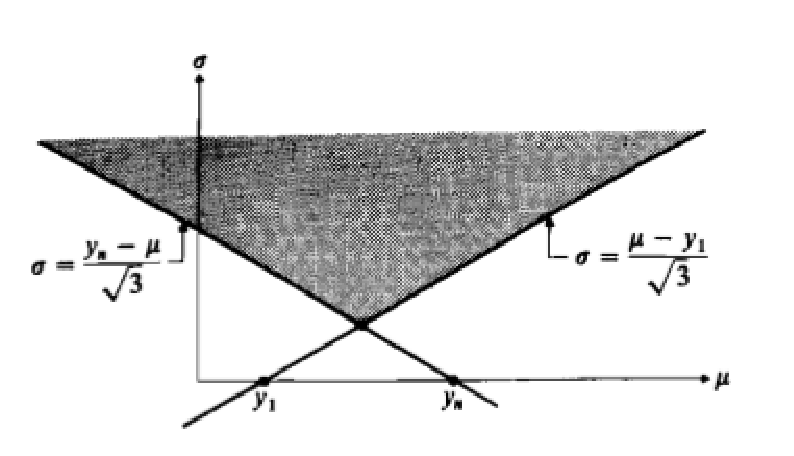
\includegraphics[scale = 0.5]{pictures/uniform_illustration.eps}
\caption{Konvergence k normálnímu rozdělení}
\label{uniform-illustration}
\end{figure}

Hodnota $(2 \sqrt{3} \sigma)^{-n}$ nabývá maxima pro minimální $\sigma$, které leží v průsečíku přímek $\mu - \sqrt{3} \sigma = y_1$ a $\mu + \sqrt{3} \sigma = y_n$. Proto odhady pro $\mu$ a $\sigma$ založené na funkci maximální věrohodnosti jsou
\begin{equation*}
\hat{\mu} = \frac{1}{2}(y_1 + y_n)
\end{equation*}
a
\begin{equation*}
\hat{\sigma} = \frac{1}{2 \sqrt{3}}(y_n - y_1)
\end{equation*}
\end{example}

\begin{theorem}[Invariance funkce odhadu metody maximální věrohodnosti]
Nechť $\hat{\Theta} = \zeta(X_1, ..., X_n)$ představuje funkci odhadu metody maximální věrohodnosti pro parametr $\theta$ pravděpodobnostní funkce $f(x, \theta)$. Předpokládejme, že $\theta$ je jednorozměrné. Dále uvažujme funkci $\tau(\cdot)$, k níž existuje jednorozměrná inverzní funkce. Pak platí, že funkce odhadu metody maximální věrohodnosti $\tau(\theta)$ je $\tau(\hat{\Theta})$.
\end{theorem}

\begin{example}
Uvažujme normální rozdělení s danou střední hodnotou $\mu_0$. Funkce odhadu parametru $\sigma^2$ je
\begin{equation*}
\hat{\Theta} = \frac{1}{n}\sum_{i = 1}^n (X_i - \mu_0)^2
\end{equation*}
Funkce odhadu parametru $\ln(\sigma^2)$ je pak
\begin{equation*}
\ln(\hat{\Theta}) = \ln\left(\frac{1}{n} \sum_{i = 1}^n (X_i - \mu_0)^2 \right)
\end{equation*}
\end{example}

Výše uvedenou větu lze dále zobecnit. Nechť $\theta = (\theta_1, ..., \theta_k)$ je $k$-rozměrný parametr a $\overline{\underline{\Theta}}$ představuje množinu všech možných $\theta$. Předmětem našeho zájmu je  odhad $\tau(\theta) = (\tau_1(\theta, ..., \tau_r(\theta))$, kde $1 \le r \le k$. Nechť $T$ představuje obor hodnot trasformace $\tau(\cdot) = (\tau_1(\cdot), ..., \tau_r(\cdot))$. To znamená, že $T$ je $r$-rozměrným prostorem. Definujme $M(\tau, x_1, ..., x_n) = \sup_{\{\theta: \tau(\theta) = \tau\}}L(\theta, x_1, ..., x_n)$\footnote{Označení $\sup$ v této knize má shodný význam jako v matematice. Čtenáři, kteří nejsou s tímto označením srozuměni, si namísto něj mohou dosadit pojmem $\max$.}. Tímto se dostáváme k následující větě.

\begin{theorem}
Uvažujme pravděpodobnostní funkci $f(\cdot, \theta_1, ..., \theta_k)$. Nechť $\hat{\Theta} = (\hat{\Theta}_1, ..., \hat{\Theta}_k)$, kde $\hat{\Theta}_j = \zeta_j(X_1, ..., X_n)$, je funkcí odhadu pro $\theta = (\theta_1, ..., \theta_k)$ dle metody maximální věrohodnosti. Nechť $\tau(\theta) = (\tau_1(\theta), ..., \tau_r(\theta))$ pro $1 \le r \le k$ představuje transformaci prostoru parametrů $\overline{\underline{\Theta}}$. Pak funkce odhadu pro $\tau(\theta) = (\tau_1(\theta), ..., \tau_r(\theta))$ dle metody maximální věrohodnosti má tvar $\tau(\hat{\Theta}) = (\tau_1(\hat{\Theta}), ..., \tau_r(\hat{\Theta}))$.
\end{theorem}

\begin{proof}
Nechť $\hat{\theta} = (\hat{\theta}_1, ..., \hat{\theta}_k)$ je odhadem pro $\theta = (\theta_1, ..., \theta_k)$. Stačí dokázat, že $M(\tau(\hat{\theta}), x_1, ..., x_n) \ge M(\tau, x_1, ..., x_n)$ pro libovolné $\tau \in T$. To vyplývá z nerovnosti $M(\tau, x_1, ..., x_n) = \sup_{\{\theta: \tau(\theta) = \tau \}}L(\theta, x_1, ..., x_n) \le \sup_{\theta \in \overline{\underline{\Theta}}} L(\theta, x_1, ..., x_n) = L(\hat{\theta}, x_1, ..., x_n) = \sup_{\{\theta: \tau(\theta) = \tau(\hat{\theta})\}}L(\theta, x_1, ..., x_n) = M(\tau(\hat{\theta}), x_1, ..., x_n)$.
\end{proof}

\begin{example}
Pro normální rozdělení platí $\theta = (\theta_1, \theta_2) = (\mu, \sigma^2)$. Uvažujme $\tau(\theta) = \mu + z_q\sigma$ kde $\phi(z_q) = q$ a $\tau(\theta)$ tak představuje $q$-tý kvantil. Dle výše uvedené věty je funkce odhadu pro $\tau(\theta)$ založená na metodě maximální věrohodnosti definována jako
\begin{equation*}
\overline{X} + z_q \sqrt{\frac{1}{n} \sum_{i = 1}^n (X_i - \overline{X})^2}
\end{equation*}
\end{example}

\subsection{Ostatní metody}

Existuje řada dalších metod bodového odhadu. Mezi tyto metody patří (a) metoda nejmenších čtverců, (b) Bayesova metoda, (c) chi-kvadrát metoda a (d) metoda nejmenší vzdálenosti. První dvě metody probereme později. V této kapitole se zaměříme na poslední dvě.

\subsubsection{Chi-kvadrát metoda}

Uvažujme náhodný výběr $X_1, ..., X_n$ z populace $f_X(x, \theta)$. Nechť $\mathscr{S}_1, ..., \mathscr{S}_k$ představuje rozpětí náhodné veličiny $X$ rozdělené na $k$ disjunktních intervalů. Pokusme se stanovit pravděpodobnost $p_j(\theta)$, s jakou pozorování připadne intervalu $\mathscr{S}_j$, kde $j = 1, ..., k$.

Jestliže je $f_X(x, \theta)$ pravděpodobnostní funkcí spojité náhodné veličiny, pak $p_j(\theta) = P[X ~ \textit{připadne intervalu} ~ \mathscr{S}_j] = \int_{\mathscr{S}_j}f_X(x, \theta) dx$. Z definice je zřejmé, že $\sum_{j = 1}^k p_j(\theta) = 1$. Nechť náhodná veličina $N_j$ představuje počet $X_i$ v náhodném výběru, která připadnou intervalu $\mathscr{S}_j$. Pak $\sum_{j = 1}^k N_j = n$, kde $n$ představuje velikost náhodného výběru. Definujme následující sumu
\begin{equation*}
\chi^2 = \sum_{j = 1}^k \frac{[n_j - n p_j(\theta)]^2}{n p_j(\theta)}
\end{equation*}
kde $n_j$ je hodnota náhodné veličiny $N_j$. Čitatel výše uvedené sumy je součtem kvadrátů rozdílu mezi skutečným a očekávaným počtem pozorování, která připadla intervalu $\mathscr{S}_j$. Odhad $\theta$ založený na chi-kvadrat metodě je takové $\hat{\theta}$, které minimalizuje $\chi^2$. Jedná se tedy o takové $\theta$ mezi všemi možnými $\theta$, pro které počet očekávaných pozorování ``nejbližší'' skutečnému počtu pozorování. Je zřejmé, že odhad $\hat{\theta}$ záleží na konkrétním výběru $\mathscr{S}_1, ..., \mathscr{S}_k$.

\begin{example}
Uvažujme náhodný výběr $X_1, ..., X_n$ z Bernoulliho rozdělení. Pravděpodobnostní funkce má tedy tvar $f_X(x, \theta) = \theta^x(1 - \theta)^{1 - x}$ pro $x = 0, 1$. Náhodná veličina $N_j$ představuje počet pozorování rovných $j = 0, 1$. Proto
\begin{gather*}
\chi^2 = \sum_{j = 0}^1 \frac{[n_j - n p_j(\theta)]^2}{n p_j(\theta)} = \frac{[n_0 - n(1 - \theta)]^2}{n(1 - \theta)} + \frac{(n_1 - n \theta)^2}{n \theta}\\
= \frac{[n - n_1 - n(1 - \theta)]^2}{n(1 - \theta)} + \frac{(n_1 - n \theta)^2}{n \theta} = \frac{(n_1 - n \theta)^2}{n} \frac{1}{\theta(1 - \theta)}
\end{gather*}
Minimum $\chi^2$ jako funkce $\theta$ nastavá v $\chi^2 = 0$ pro $\theta = \frac{n_1}{n}$. Proto $\hat{\theta} = \frac{n_1}{n}$.
\end{example}

Někdy je složité nalézt $\hat{\theta}$, které minimalizuje $\chi^2$. Proto bývá často $n p_j(\theta)$ ve jmenovateli nahrazeno $n_j$\footnote{Pokud $n_j = 0$, pak namísto $n_j$ použijeme 1.}. Pak hovoříme o tzv. modifikovaném $\chi^2$, které je definováno jako
\begin{equation*}
\chi^2_{mod} = \sum_{j = 1}^k \frac{[n_j - np_j(\theta)]^2}{n_j}
\end{equation*}
Tento modifikovaný odhad je opět založen na hodnotě $\hat{\theta}$, která minimalizuje $\chi^2_{mod}$.

\subsubsection{Metoda minimální vzdálenosti}

Nechť $X_1, ..., X_n$ představuje náhodný výběr z populace s kumulativní distribuční funkcí $F(X, \theta)$. Definujme funkci $d(F, G)$, která představuje vzdálenost mezi dvěma kumulativními distribučními funkcemi $F$ a $G$. Příkladem takovéto funkce může být $\sup_x|F(x) - G(x)|$, která představuje největší vertikální vzdálenost mezi funkcemi $F$ a $G$ a je ilustrována obrázkem (\ref{min-distance-function}).

\begin{figure}[htp]
\centering
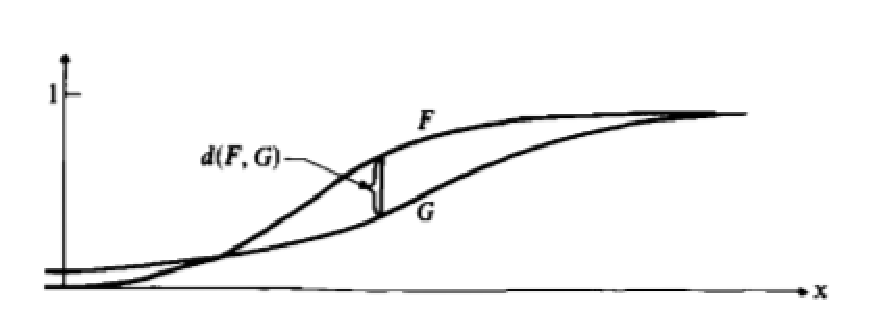
\includegraphics[scale = 0.5]{pictures/min_distance_function.eps}
\caption{Vzdálenost mezi dvěma kumulativními pravděpodobnostními funkcemi}
\label{min-distance-function}
\end{figure}

Odhad $\hat{\theta}$ parametru $\theta$ získaný pomocí metody minimální vzdálenosti je tedy představován takovou hodnotou, která minimalizuje $d(F(x, \theta), F_n(x))$, kde $F_n(x)$ je výběrovou kumulativní distribuční funkcí\footnote{Pouze připomeňme, že na základě teorie velkých čísel konverguje výběrová kumulativní distribuční funkce $F_n(x)$ ke kumulativní distribuční funkci $F(x)$ dané populace.}. Bohužel ne vždy je snadné určit hodnotu $\hat{\theta}$, která minimalizuje funkci vzdálenosti $d(F(x, \theta), F_n(x))$. Následující příklad je v tomto směru vyjímkou.

\begin{proof}
Nechť $X_1, ..., X_n$ představuje náhodný výběr z Bernoulliho rozdělení. Pak platí
\begin{equation*}
F(x, \theta) = (1 - \theta)I_{[0, 1)}(x) + I_{[1, \infty)}(x)
\end{equation*}
kde $0 \le \theta \le 1$. Dále nechť $n_j$ představuje počet pozorování rovných $j$, kde $j = 0, 1$. Pak zjevně platí
\begin{equation*}
F_n(x) = \frac{n_0}{n}I_{[0, 1)}(x) + I_{[1, \infty)}(x)
\end{equation*}
Jestliže použijeme funkci vzdálenosti $d(F,G) = \sup_x |F(x) - G(x)|$, pak tato funkce nabývá minima v bodě $1 - \theta = \frac{n_0}{n}$ neboli $\theta = \frac{n_1}{n} = \sum \frac{x_i}{n}$. Proto $\hat{\theta} = \overline{x}$.
\end{proof}.

\section{Vlastnosti funkcí odhadu}

V předchozím textu jsme ukázali několik metod bodového odhadu. Tímto vyvstává přirozená otázka, která z těchto metod je v dané situaci nejvhodnější.

\subsection{Blízkost funkce odhadu}

Uvažujme náhodný výběr $X_1, ..., X_n$ z populace $f(x, \theta)$. Funkce odhadu $\tau(\theta)$ je statistika, řekněme $\mathfrak{t}(X_1, ..., X_n)$, jejíž hodnota je použita jako odhad $\tau(\theta)$. V ideálním případě bychom chtěli, aby hodnota $\mathfrak{t}(X_1, ..., X_n)$ byla rovna hledané hodnotě $\tau(\theta)$. To však, s vyjímkou několika triviální případů, není možné.

\begin{example}
Uvažujme náhodný výběr z populace $f(x, \theta) = I_{(\theta - \frac{1}{2}, \theta + \frac{1}{2})}(x)$, kde $\theta$ je přirozené číslo. Je zřejmé, že $\theta$ je možné přesně odhadnout na základě jednoho pozorování $x_1$ a to tak, že $\mathfrak{t}(x_1)$ bude představovat hodnotu přirozeného čísla nejbližšího $x_1$.
\end{example}

Vzhledem k tomu, že $\mathfrak{t}(X_1, ..., X_n)$ není ve většině případů přesným odhadem $\tau(\theta)$, požadujeme, aby bylo alespoň ``blízkým'' odhadem. $T = \mathfrak{t}(X_1, ..., X_n)$ je statistika, která sleduje určité pravděpodobnostní rozdělení. Proto je logické požadovat, aby se hodnoty $t$ náhodné veličiny $T$ ``koncentrovaly'' poblíž $\tau(\theta)$.

\begin{definition}[Koncentrovaná a nejkoncentrovanější funkce odhadu]
Uvažujme dvě funkce odhadu $T = \mathfrak{t}(X_1, ..., X_n)$ a $T' = \mathfrak{t}'(X_1, ..., X_n)$ pro $\tau(\theta)$. Říkáme, že $T'$ je více koncentrované než $T$, jestliže
\begin{equation*}
P_{\theta}[\tau(\theta) - \lambda < T' \le \tau(\theta) + \lambda] \ge P_{\theta}[\tau(\theta) - \lambda < T \le \tau(\theta) + \lambda]
\end{equation*}
pro všechna $\lambda > 0$ a každé $\theta$ z $\overline{\underline{\Theta}}$. Funkci odhadu $T^* = \mathfrak{t}^*(X_1, ..., X_n)$ nazýváme nejkoncentrovanější funkcí odhadu, jestliže je více koncentrovaná než libovolná jiná funkce odhadu.
\end{definition}

Ve výše uvedené definici jsme použili značení $P_{\theta}[\cdot]$, abychom zdůraznili, že pravděpodobnost $P_{\theta}[\tau(\theta) - \lambda < T \le \tau(\theta) + \lambda]$ závisí na $\theta$ skrze pravděpodobnostní rozdělení $T$.

Vedle koncentrované a nejkoncentrovanější funkce odhadu existuje také obdobná Pitmanova definice blízké a nejbližší funkce odhadu.

\begin{definition}[Blízká a nejbližší funkce odhadu]
Uvažujme dvě funkce odhadu $T = \mathfrak{t}(X_1, ..., X_n)$ a $T' = \mathfrak{t}'(X_1, ..., X_n)$ pro $\tau(\theta)$. Říkáme, že $T'$ je více koncentrované než $T$, jestliže
\begin{equation*}
P_{\theta}[|T' - \tau(\theta)| < |T - \tau(\theta)|] \ge \frac{1}{2}
\end{equation*}
pro každé $\theta$ z $\overline{\underline{\Theta}}$. Funkci odhadu $T^* = \mathfrak{t}^*(X_1, ..., X_n)$ nazýváme nejbližší funkcí odhadu, jestliže je bližší než libovolná jiná funkce odhadu.
\end{definition}

Základní slabinou výše uvedených definic je skutečnost, že nejkoncentrovanější resp. nejbližší funkce odhadu existuje pouze ve vyjímečných případech. Důvodem je existence přílišného množství možných funkcí odhadu, než aby bylo možné některou z nich prohlásit za nejvhodnější. Navíc velmi často nelze ani tvrdit, že jedna funkce  odhadu je koncentrovanější resp. bližší než jiná, protože to se obvykle odvíjí od konkrétní hodnoty parametru $\theta$.

V předchozím textu jsme uvažovali fixní velikost náhodného výběru. Z pohledu ``blízkosti'' funkce odhadu je však také důležité, aby se přesnost odhadu zlepšovala s rostoucí velikostí náhodného výběru. V souvislosti s náhodným vzorkem dané velikosti hovoříme o vlastnostech funkce odhadu jako o vlastnostech malého výběru. O vlastnostech funkce odhadu, které jsou definované pro rostoucí velikost náhodného výběru, pak hovoříme jako o vlastnostech velkého výběru.

\subsection{Střední chyba čtverců}

\begin{definition}[MSE (mean-squared error) - střední chyba čtverců]
Nechť $T = \mathfrak{t}(X_1, ..., X_n)$ je funkcí odhadu pro $\tau(\theta)$. Pak $E_{\theta}[(T - \tau{\theta})^2]$ nazýváme MSE pro funkci odhadu $T = \mathfrak{t}(X_1, ..., X_n)$ a značíme ji jako $MSE_{\mathfrak{t}}(\theta)$.
\end{definition}

$\theta$ v případě $E_{\theta}[\cdot]$ indikuje pravděpodobnostní funkci, ze které pochází náhodný výběr. To znamená, že
\begin{gather*}
E_{\theta}[(T - \tau(\theta))^2] = E_{\theta}[(\mathfrak{t}(X_1, ..., X_n) - \tau(\theta))^2]\\
= \int \cdots \int (\mathfrak{t}(x_1, ..., x_n) - \tau(\theta))^2 f(x_1, \theta) \cdots f(x_n, \theta) dx_1 \cdots dx_n
\end{gather*}
kde $f(x, \theta)$ představuje pravděpodobnostní funkci populace.

Pokud porovnáváme funkce odhadu pomocí MSE, vybereme funkci s nejmenší MSE. Teoreticky je tak možné definovat funkci odhadu s nejmenší MSE, avšak stejně jako v předchozím případě, i zde je spíše vyjímkou, pokud takováto funkce existuje.

\begin{example}
Nechť $X_1, ..., X_n$ představuje náhodný výběr z $f(x, \theta)$, kde $\theta$ je reálné číslo. Předpokládejme, že předmětem zájmu je odhad parametru $\theta$, tj. $\tau(\theta) = \theta$.

Hledáme tedy funkci odhadu $T^* = \mathfrak{t}^*(X_1, ..., X_n)$ takovou, že $MSE_{\mathfrak{t}^*}(\theta) \le MSE_{\mathfrak{t}}(\theta)$ pro každé $\theta$ a libovolné $T = \mathfrak{t}(X_1, ..., X_n)$. Uvažujme rodinu funkcí odhadu $T_{\theta_0} = \mathfrak{t}_{\theta_0}(X_1, ..., X_n) \equiv \theta_0$ pro $\theta_0 \in \overline{\underline{\Theta}}$. Pro libovolné $\theta_0$ z $\overline{\underline{\Theta}}$ tedy funkce odhadu $T_{\theta_0}$ ``ignoruje'' pozorování a parametru $\theta$ přímo přiřadí hodnotu $\theta_0$. Všimněme si, že
\begin{equation*}
MSE_{\mathfrak{t}_{\theta_0}}(\theta) = E_{\theta}[(\mathfrak{t}(X_1, ..., X_n) - \theta)^2] = E_{\theta}[(\theta_0 - \theta)^2] = (\theta_0 - \theta)^2
\end{equation*}
Proto $MSE_{\mathfrak{t}_{\theta_0}}(\theta_0) = 0$. Má-li tedy existovat $T^* = \mathfrak{t}^*(X_1, ..., X_n)$, které splňuje $MSE_{\mathfrak{t}^*}(\theta) \le MSE_{\mathfrak{t}}(\theta)$ pro každé $\theta$ a funkci $\mathfrak{t}$, pak $MSE_{\mathfrak{t}^*} \equiv 0$. Aby funkce bodového odhadu $\mathfrak{t}^*$ měla MSE rovnu nule, musí parametr $\theta$ odhadnout vždy správně. To znamená, že musí být z náhodného výběru schopna vždy určit správnou hodnotu parametru $\theta$.
\end{example}

Jedním z důvodů, proč nejsme schopni nalézt funkci odhadu s nejmenší chybou čtverců je skutečnost, že počet potenciálních funkcí je příliš veliký. Tato množina pocentiálních funkcí také zahrnuje funkce, které jsou extrémně ``předpojaté'' ve prospěch určité konkrétní hodnoty parametru $\theta$\footnote{Jako ilustrace může posloužit funkce $\mathfrak{t}_{\theta_0}(X_1, ..., X_n)$ z předchozího příkladu, která byla ``předpojatá'' ve prospěch parametru $\theta_0$. Tato funkce totiž bez ohledu na reálný výsledek pozorování stanovila hodnotu parametru $\theta$ vždy rovnu $\theta_0$.}. Proto je vhodné množinu všech potencionálních funkcí odhadu omezit další podmínkou. Touto další podmínkou je podmínka nezkreslení.

\begin{definition}[Nezkreslená funkce odhadu]
O funkci odhadu $T = \mathfrak{t}(X_1, ..., X_n)$ říkáme, že je nezkreslená, tehdy a jen tehdy, jestliže
\begin{equation*}
E_{\theta}[T] = E_{\theta}[\mathfrak{t}(X_1, ..., X_n)] = \tau(\theta)
\end{equation*}
pro všechna $\theta = \overline{\underline{\Theta}}$.
\end{definition}

\begin{example}
Je tedy zřejmé, že funkce odhadu $\mathfrak{t}_{\theta_0}(X_1, ..., X_n)$ z předchozího příkladu není nezkreslenou funkcí odhadu parametru $\theta$, protože
\begin{equation*}
E_{\theta}[\mathfrak{t}_{\theta_0}(X_1, ..., X_n)] = E_{\theta}[\theta_0] = \theta_0 \neq \theta
\end{equation*}
\end{example}

\begin{corollary}
Jestliže je $T$ nezkreslenou funkcí odhadu pro $\tau(\theta)$, pak platí
\begin{equation*}
MSE_{\mathfrak{t}}(\theta) = D[T]
\end{equation*}
Toto tvrzení vyplývá ze vztahu
\begin{equation*}
MSE_{\mathfrak{t}}(\theta) = D[T] + (\tau(\theta) - E_{\theta}[T])^2
\end{equation*}
\end{corollary}

\begin{proof}
\begin{gather*}
MSE_{\mathfrak{t}}(\theta) = E_{\theta}[(T - \tau(\theta))^2] = E_{\theta}\left[\left((T - E_{\theta}[T]) - (\tau(\theta) - E_{\theta}[T])\right)^2 \right]\\
= E_{\theta}[(T - E_{\theta}[T])^2] - 2(\tau(\theta) - E_{\theta}[T])E_{\theta}[T - E_{\theta}[T]] + E_{\theta}[(\tau(\theta) - E_{\theta}[T])^2]\\
= D[T] + (\tau(\theta) - E_{\theta}[T])^2
\end{gather*}
\end{proof}

Člen $\tau(\theta) - E_{\theta}[T]$ nazýváme zkreslením funkce odhadu $T$. Tento člen může být kladný, záporný ale i nulový.

\begin{example}
Uvažujme náhodný výběr $X_1, ..., X_n$ z $f(x, \theta) = \phi_{\mu, \sigma^2}(x)$. Z příkladu (7.5) víme, že funkce odhadu dle metody maximální věrohodnosti pro parametr $\mu$ resp. $\sigma$ je $\overline{X}$ resp. $\frac{1}{n}\sum (X_i - \overline{X})^2$. Platí $E_{\theta}[\overline{X}] = \mu$, a proto je $\overline{X}$ nezkreslenou funkcí odhadu pro $\mu$. MSE funkce $\overline{X}$ je
\begin{equation*}
E_{\theta}[(\overline{X} - \mu)^2] = D[\overline{X}] = \frac{\sigma^2}{n}
\end{equation*}
Z předchozího textu také víme, že $E_{\theta}[S_n^2] = \sigma^2$, a proto
\begin{gather*}
E_{\theta}\left[\frac{1}{n} \sum_{i = 1}^n (X_i - \overline{X})^2 \right] = \frac{n - 1}{n}E_{\theta}\left[\frac{1}{n - 1} \sum_{i = 1}^n (X_i - \overline{X})^2 \right]\\
\frac{n - 1}{n}E[S_n^2] = \frac{n - 1}{n} \sigma^2
\end{gather*}
Funkce odhadu pro $\sigma$ tak je zkreslená. MSE pro $\frac{1}{n} \sum (X_i - \overline{X})^2$ lze s pomocí věty (6.2) vyjádřit jako
\begin{gather*}
E_{\theta}\left[\left(\frac{1}{n} \sum_{i = 1}^n (X_i - \overline{X})^2 - \sigma^2 \right)^2 \right] = D\left[\frac{1}{n} \sum_{i = 1}^n (X_i - \overline{X})^2 \right] + \left(\sigma^2 - E_{\theta}\left[\frac{1}{n} \sum_{i = 1}^n (X_i - \overline{X})^2 \right] \right)^2\\
= \frac{(n - 1)^2}{n^2}D[S_n^2] + \left(\sigma^2 - \frac{n - 1}{n} \sigma^2 \right)^2 = \frac{(n - 1)^2}{n^2}\frac{1}{n}\left(\mu_4 - \frac{n - 3}{n - 1}\sigma^4 \right) + \frac{\sigma^4}{n^2}
\end{gather*}
\end{example}

V následujícím textu bude MSE hlavním nástrojem pro posouzení funkce odhadu.

\subsection{Konzistentnost a BAN}

\begin{definition}[Konzistentnost ve smyslu MSE]
Nechť $T_1, ..., T_n$ představuje posloupnost funkcí odhadu pro $\tau(\theta)$, kde $T_n = \mathfrak{t}_n(X_1, ..., X_n)$ je definováno pro náhodný výběr velikosti $n$. Tuto posloupnost funkcí odhadu označujeme jako konzistentní ve smyslu MSE pouze tehdy a jen tehdy, jestliže
\begin{equation*}
\lim_{n \rightarrow \infty} E_{\theta}[(T_n - \tau(\theta))^2] = 0
\end{equation*}
pro všechna $\theta$ z $\overline{\underline{\Theta}}$.
\end{definition}

Konzistentnost ve smyslu MSE mimojiné znamená, že zkreslení a rozptyl $T_n$ se blíží nule s tím, jak se $n$ blíží nekonečnu, protože $E_{\theta}[(T_n - \tau(\theta))^2] = D[T_n] + (\tau(\theta) - E_{\theta}[T_n])^2$.

\begin{example}
Uvažujme náhodný výběr z pravděpodobnostního rozdělení se střední hodnotou $\mu$ a rozptylem $\sigma^2$. Nechť $\overline{X}_n = \frac{1}{n}\sum_{i = 1}^n X_i$ představuje posloupnost funkcí odhadu pro $\mu$ a $S_n^2 = \frac{1}{n - 1} \sum_{i = 1}^n (X_i - \overline{X}_n)$ pak posloupnost funkcí odhadu pro $\sigma^2$. Platí
\begin{equation*}
\lim_{n \rightarrow \infty} E[(\overline{X}_n - \mu)^2] = \lim_{n \rightarrow \infty} D[\overline{X}_n] = \lim_{n \rightarrow \infty} \frac{\sigma^2}{n} = 0
\end{equation*}
a proto je posloupnost $\{\overline{X}_n\}$ konzistení funkcí odhadu pro $\mu$. Dále platí
\begin{equation*}
\lim_{n \rightarrow \infty} E[(S_n^2 - \sigma^2)^2] = \lim_{n \rightarrow \infty} D[S_n^2] = \lim_{n \rightarrow \infty} \frac{1}{n} \left(\mu_4 - \frac{n - 3}{n - 1} \right) = 0
\end{equation*}
a proto také $\{S_n^2\}$ představuje konzistentní posloupnost funkcí odhadu pro $\sigma^2$. Všimněme si, že je-li $T_n = \frac{1}{n} \sum (X_i - \overline{X})^2$, pak je posloupnost $\{T_n\}$ konzistentní funkcí odhadu ve smyslu MSE nejen pro $\mu$ ale také pro $\sigma^2$.
\end{example}

Vedle výše uvedené definice existuje také ``slabší'' forma konzistence.

\begin{definition}[Slabší forma konzistence ve smyslu MSE]
Uvažujme posloupnost $T_1, ..., T_n$ funkcí odhadu pro $\tau(\theta)$, kde $T_n = \mathfrak{t}_n(X_1, ..., X_n)$. Posloupnost $\{T_n\}$ nazýváme ``slabě''  konzistentní ve smyslu MSE, jestliže je pro každé $\epsilon > 0$ a $\theta \in \overline{\underline{\Theta}}$ platí
\begin{equation*}
\lim_{n \rightarrow \infty} P_{\theta}[\tau(\theta) - \epsilon < T_n < \tau(\theta) + \epsilon] = 1
\end{equation*}
\end{definition}

\begin{proof}
S použitím Chebyshevovy nerovnosti lze dokázat
\begin{gather*}
P_{\theta}[\tau(\theta) - \epsilon < T_n < \tau(\theta) + \epsilon] = P[|T_n - \tau(\theta)| < \epsilon]\\
= P_{\theta}[(T_n - \tau(\theta))^2 < \epsilon^2] \ge 1 - \frac{E_{\theta}[(T_n - \tau(\theta))^2]}{\epsilon^2}
\end{gather*}
S tím, jak se $n$ blíží nekonečnu, se $E_{\theta}[(T_n - \tau(\theta))^2]$ blíží nule. Proto
\begin{equation*}
\lim_{n \rightarrow \infty} P_{\theta}[\tau(\theta) - \epsilon < T_n < \tau(\theta) + \epsilon] = 1
\end{equation*}
\end{proof}

Jestliže je funkce dhadu konzistentní, pak je také slabě konzistentní. Opačné tvrzení však neplatí.

\begin{definition}[BAN (best asymptotically normal) funkce odhadu]
Posloupnost funkcí bodového odhadu $T_1^*, ..., T_n^*$ pro $\tau(\theta)$ nazýváme BAN (best asymptotically normal), jestliže splňuje následující čtyři podmínky
\begin{enumerate}
\item Pravděpodobnostní rozdělení $\sqrt{n}[T_n^* - \tau(\theta)]$ se blíží normálnímu rozdělení s nulovou střední hodnotou a rozptylem $\sigma^{*2}(\theta)$ s tím, jak se $n$ blíží nekonečnu.
\item Pro každé $\epsilon > 0$ a každé $\theta \in \overline{\underline{\Theta}}$ platí
\begin{equation*}
\lim_{n \rightarrow \infty} P_{\theta}[|T^*_n - \tau(\theta)| > \epsilon] = 0
\end{equation*}
\item Nechť $\{T_n\}$ představuje libovolnou alternativní posloupnost slabě konzistentních funkcí odhadu s pravděpodobnostním rozdělením $\sqrt{n}[T_n - \tau(\theta)]$, které se blíží normálnímu rozdělení s nulovou střední hodnotou a rozptylem $\sigma^2(\theta)$.
\item $\sigma^2(\theta)$ není menší než $\sigma^{*2}(\theta)$ pro libovolný otevřený interval hodnot $\theta$.
\end{enumerate} 
\end{definition}

Namísto označení BAN se někdy používá CANE (consistent asymptotically normal efficient).

\begin{example}
Pro náhodné výběry z normálního rozdělení se střední hodnotou $\mu$ a rozptylem $\sigma^2$, je posloupnost $T^*_n = \frac{1}{n} \sum_{i = 1}^n X_i = \overline{X}_n$ je posloupností BAN pro $\mu$. Limitní pravděpodobnostní funkcí $\sqrt{n}(\overline{X}_n - \mu)$ je normální rozdělení s nulovou střední hodnotou a rozptylem $\sigma^2$. Žádná jiná funkce bodového odhadu nemůže mít menší rozptyl pro libovolný interval hodnot $\mu$. Nicméně existují i jiné BAN funkce bodového odhadu pro $\mu$, které mají shodné limitní normální rozdělení. Jako příklad uveďme
\begin{equation*}
T'_n = \frac{1}{n + 1} \sum_{i = 1}^n X_i
\end{equation*}
\end{example}

\subsection{Ztrátová a riziková funkce}

\begin{definition}[Ztrátová funkce]
Uvažujme odhad parametru $\tau(\theta)$. Nechť $t$ označuje hodnotu odhadu pro $\tau(\theta)$. Ztrátová funkce $\mathfrak{l}(t, \theta)$ je reálná funkce, která splňuje
\begin{enumerate}
\item $\mathfrak{l}(t, \theta) \ge 0$ pro všechny možné odhady $t$ a všechna $\theta \in \underline{\overline{\Theta}}$,
\item $\mathfrak{l}(t, \theta) = 0$ pro $t = \tau(\theta)$
\end{enumerate}
\end{definition}

Z logiky věci vyplývá, že ztrátová funkce by měla vracet  větší hodnoty pro větší odchylky $t$ od skutečné hodnoty $\tau(\theta)$ a naopak. Několik možných ztrátových funkcí je uvedeno v následujícím příkladu.

\begin{example}
~
\begin{enumerate}
\item $\mathit{l_1}(t, \theta) = (t - \tau(\theta))^2$
\item $\mathit{l_2}(t, \theta) = |t - \tau(\theta)|^2$
\item $\mathit{l_3}(t, \theta) = \begin{cases}A ~~~ \textit{pro} ~ |t - \tau{theta}| > \epsilon\\ 0 ~~~ \textit{pro} ~ |t - \tau{theta}| \le \epsilon \end{cases}$, kde $A > 0$
\item $\mathit{l_4}(t, \theta) = \rho(\theta)|t - \tau(\theta)|^r$ pro $\rho(\theta)$ a $r > 0$
\end{enumerate}
Funkce $\mathfrak{l}_1$ se nazývá ztrátová funkce chyby čtverců a funkce $\mathfrak{l}_2$ se nazývá ztrátová funkce absolutní chyby. Jak $\mathit{f}_1$ tak $\mathit{f}_2$ je rostoucí funkce chyby $t - \tau(\theta)$. Naproti tomu funkce $\mathfrak{l}_3$ nabývá pouze hodnot $A$ a 0 v závislosti na tom, zda-li se chyba $t- \tau(\theta)$ nachází v intervalu $\tau(\theta) \pm \epsilon$ či nikoliv. Konečně funkce $\mathfrak{l}_4$ je obecnou formou ztrátové funkce, která zahrnuje $\mathfrak{l}_1$ a $\mathfrak{l}_2$ jako specifické případy.
\end{example}

Při odhadu parametrů je naším cílem zvolit takovou funkci odhadu $T = \mathfrak{t}(X_1, ..., X_n)$, která bude minimalizovat ztrátovou funkci\footnote{Předpokládáme, že ztrátovou funkci známe. Volba vhodné ztrátové funkce však nemusí být tak jednoduchá, jak by se mohlo na první pohled zdát.}. Ztrátová funkce závisí na $t$, což je hodnota funkce bodového odhadu $T$. To znamená, že se hodnota ztrátové funkce odvíjí od konkrétního náhodného výběru $X_1 = x_1, ..., X_n = x_n$. Je zřejmé, že ztrátovou funkci nemůžeme minimalizovat pro každý možný náhodný výběr, avšak můžeme se ji pokusit minimalizovat v ``průměru''. Tímto se dostáváme k tzv. rizikové funkci.

\begin{definition}[Riziková funkce]
Pro danou ztrátovou funkci $\mathfrak{l}(t, \theta(t))$ a funkci bodového odhadu $T = \mathfrak{t}(X_1, ..., X_n)$ je riziková funkce definována jako
\begin{equation*}
\mathfrak{r}_t(\theta) = E_{\theta}[\mathfrak{t}(T, \theta)]
\end{equation*}
Riziková funkce tak představuje průměrnou hodnotu ztrátové funkce.
\end{definition}

Rizikovou funkci lze v zásadě vypočíst dvěma způsoby. Prvním z nich je pomocí sdružené pravděpodobnostní funkce náhodného výběru
\begin{gather*}
E_{\theta}[\mathfrak{l}(T, \theta)] = E_{\theta}[\mathfrak{l}(\mathfrak{t}(X_1, ..., X_n), \theta)]\\
= \int \cdots \int \mathfrak{l}(\mathfrak{t}(x_1, ..., x_n), \theta) \prod_{i = 1}^n f(x_i, \theta) d x_i
\end{gather*}
Druhý způsob se pak opírá o $T$ a její pravděpodobnostní funkci
\begin{gather*}
E_{\theta}[\mathfrak{l}(T, \theta)] = \int \mathfrak{l}(\cdot, \theta)f_T(t)dt
\end{gather*}

\begin{example}
Uvažujme ztrátové funkce z předchozího příkladu. Odpovídající rizikové funkce jsou
\begin{enumerate}
\item $E_{\theta}[(T - \tau(\theta))^2]$, což je již dříve uvedená MSE
\item $E_{\theta}[|T - \tau(\theta)|]$
\item $A \cdot P_{\theta}[|T - \tau(\theta)| > \epsilon]$
\item $\rho(\theta) E_{\theta}[|T - \tau(\theta)|^r]$
\end{enumerate}
\end{example}

\begin{definition}[Přijatelná funkce odhadu]
Uvažujme dvě funkce odhadu $T_1 = \mathit{t_1}(X_1, ..., X_n)$ a $T_2 = \mathit{t_2}(X_1, ..., X_n)$. Funkce odhadu $\mathfrak{t}_1$ je považována za nadřazenou funkci odhadu $\mathfrak{t}_2$ tehdy a jen tehdy, jestliže
\begin{equation*}
\mathit{R_{\mathfrak{t}_1}}(\theta) \ge \mathit{r_{\mathfrak{t}_2}}(\theta)
\end{equation*}
pro všechna $\theta \in \overline{\underline{\Theta}}$ a
\begin{equation*}
\mathit{R_{\mathfrak{t}_1}}(\theta) < \mathit{r_{\mathfrak{t}_2}}(\theta)
\end{equation*}
pro alespoň jedno $\theta \in \overline{\underline{\Theta}}$.
\end{definition}

Stejně jako v předchozích případech je také ztrátová funkce funkcí parametru $\theta$. Určení nejlepší funkce odhadu tak nemusí být jednoznačné. Částečným řešením tohoto problému je koncept tzv. minimaxu.

\begin{definition}[Minimax]
Funkci bodového odhadu $t^*$ nazýváme minimaxem tehdy a jen tehdy, jestliže
\begin{equation*}
\sup_{\theta} \mathfrak{r}(t^*)(\theta) \le \sup_{\theta} \mathfrak{r}_t(\theta)
\end{equation*}
pro každou alternativní funkci odhadu $\mathfrak{t}$.
\end{definition}

\section{Dostatečnost}

\subsection{Dostatečná statistika}

Uvažujme náhodný výběr $X_1, ..., X_n$ z populace $f(\cdot, \theta)$. Statistiku jsme definovali jako funkci náhodného výběru. Definičním oborem této funkce je množina všech hodnot, jichž může náhodný výběr $X_1, ..., X_n$ nabývat, a oborem hodnot je pak reálná osa. Na statistiku $T = \mathfrak{t}(X_1, ..., X_n)$ je také možno pohlížet jako na náhodnou veličinu. Funkce $\mathfrak{t}(\cdot, ..., \cdot)$ tedy transformuje $n$ náhodných veličin $X_1, ..., X_n$ do jedné náhodné veličiny. Předmětem našeho zájmu bude, zda-li při této transformaci dochází ke ztrátě informace či nikoliv.

Nechť $\mathfrak{X}$ označuje rozpětí hodnot, jichž může nabývat $(X_1, ..., X_n)$. Pomocí statistiky lze definovat segment prostoru $\mathfrak{X}$. Uvažujme statistiku $T = \mathfrak{t}(X_1, ..., X_n)$. Libovolná pozorování $(x_1, ..., x_n)$, pro která platí $t(x_1, ..., x_n) = t_0$, totiž představují segment prostoru $\mathfrak{X}$ definovaný hodnotou $T = t_0$.

\begin{example}
Uvažujme náhodný výběr $(X_1, X_2, X_3)$ z Bernoulliho rozdělení. Prostor $\mathfrak{X}$ se skládá z osmi bodů, a to $(0,0,0), (0,0,1), (0,1,0), (1,0,0), (0,1,1), (1,1,0), (1,0,1)$ a $(1,1,1)$. Definujme statistiku $T = X_1 + X_2 + X_3$. Tato statistika může nabývat čtyř hodnot, a proto rozděluje prostor $\mathfrak{X}$ na čtyři segmenty, a to  $\{(0,0,0)\}, \{(0,0,1), (0,1,0), (1,0,0) \}, \{(0,1,1), (1,1,0), (1,0,1)\}$ a $\{(1,1,1)\}$. Prostor $\mathfrak{X}$ by na shodné čtyři segmenty rozdělily také statistiky $T = 6(x_1 + x_2 + x_3)^2$ a $T = x_1^2 + x_2^2 + x_3^2$. Jestliže by tedy naším cílem bylo ``zredukovat'' prostor $\mathfrak{X}$, poskytly by nám všechny tyto tři statistiky stejnou službu.
\end{example}

\begin{definition}[Dostatečná statistika]
Uvažujme náhodný výběr $X_1, ..., X_n$ z populace $f(\cdot, \theta)$, kde $\theta$ může představovat jak skalár tak vektor. Předpokládejme, že funkční předpis $f(\cdot, \theta)$ je nám, s vyjímkou parametru $\theta$, znám. Statistika $S = \mathfrak{s}(X_1, ..., X_2)$ je dostatečná tehdy a jen tehdy, jestliže podmníněné pravděpodobnostní rozdělení $X_1, ..., X_n$ pro dané $S = s$ není funkcí $\theta$.
\end{definition}

Dostatečná statistika tedy zredukuje prostor $\mathfrak{X}$ takovým způsobem, že nedojde ke ztrátě informace o $\theta$. Ta je obsažena v náhodném výběru $X_1, ..., X_n$, což je důsledkem požadavku, aby podmíněné pravděpodobnostní rozdělení $X_1, ..., X_n$ nezáviselo na $\theta$. Nelze tedy očekávat, že získáme informaci o $\theta$ tím, že budeme provádět náhodný výběr z pravděpodobnostního rozdělení, které není funkcí $\theta$.

\begin{example}
Nechť $X_1, X_2, X_3$ představuje náhodný výběr z Bernoulliho rozdělení. Uvažujme dvě statistiky $S = \mathfrak{s}(X_1, X_2, X_3) = X_1 + X_2 + X_3$ a $T = \mathfrak{t}(X_1, X_2, X_3) = X_1X_2 + X_3$. Ukažme, že $S$ je na rozdíl od $T$ dostatečná statistika.
\begin{table}
\begin{center}
\begin{tabular}{| c | c | c | c | c |}
\hline
 & hodnoty $S$ & hodnoty $T$ & $f_{X_1, X_2, X_3|S}$ & $f_{X_1, X_2, X_3|T}$\\
\hline
$(0,0,0)$ & $0$ & $0$ & $1$ & $\frac{1 - p}{1 + p}$\\
\hline
$(0,0,1)$ & $1$ & $1$ & $\frac{1}{3}$ & $\frac{1 - p}{1 + 2p}$\\
\hline
$(0,1,0)$ & $1$ & $0$ & $\frac{1}{3}$ & $\frac{p}{1 + p}$\\
\hline
$(1,0,0)$ & $1$ & $0$ & $\frac{1}{3}$ & $\frac{p}{1 + p}$\\
\hline
$(0,1,1)$ & $2$ & $1$ & $\frac{1}{3}$ & $\frac{p}{1 + 2p}$\\
\hline
$(1,0,1)$ & $2$ & $1$ & $\frac{1}{3}$ & $\frac{p}{1 + 2p}$\\
\hline
$(1,1,0)$ & $2$ & $1$ & $\frac{1}{3}$ & $\frac{p}{1 + 2p}$\\
\hline
$(1,1,1)$ & $3$ & $2$ & $1$ & $1$\\
\hline
\end{tabular}
\caption{Dostatečná statistika}
\label{sufficient-statistics}
\end{center}
\end{table}

První sloupec tabulky (\ref{sufficient-statistics}) přestavuje prostor $\mathfrak{X}$. Podmíněné pravděpodobnosti lze vypočíst obvyklým způsobem. Jako příklad uveďme
\begin{gather*}
f_{X_1, X_2, X_3|S = 1}(0,1,0|1) = P[X_1 = 0, X_2 = 1, X_3 = 0 | S = 1]\\
= \frac{P[X_1 = 0, X_2 = 1, X_3 = 0, S = 1]}{P[S = 1]}\\
= \frac{(1 - p)p(1 - p)}{\binom{3}{1}p(1 - p)^2} = \frac{1}{3}
\end{gather*}
a
\begin{gather*}
f_{X_1, X_2, X_3|T = 0}(0, 1, 0 | 0) = \frac{P[X_1 = 0, X_2 = 1, X_3 = 0, T = 0]}{P[T = 0]}\\
= \frac{(1 - p)^2 p}{(1 - p)^3 + 2(1 - p)^2 p} = \frac{p}{1 - p + 2p} = \frac{p}{1 + p}
\end{gather*}
Podmíněná pravděpodobnostní funkce náhodného výběru pro danou hodnotu $S = s$ je nezávislá na parametru $p$, a proto je $S$ dostatečnou statistikou. Naproti tomu podmíněná pravděpodobnostní funkce náhodného výběru pro danou hodnotu $T = t$ je funkcí parametru $p$, a proto se o dostatečnou statistiku nejedná.

Všimněme si, že redukce prostoru $\mathfrak{X}$ pomocí statistiky $T$ je výraznější než pomocí statistiky $S$. Přirozenou otázkou je, zda-li existuje dostatečná statistika, která představuje větší redukci prostoru $\mathfrak{X}$ než $S$. Odpověď zní ``ne'' a lze ji dokázat zkoumáním množin všech segmentů prostoru $\mathfrak{X}$, které rozdělí tento prostor na tři a méně částí.
\end{example}

V případě náhodného výběru z pravděpodobnostní funkce spojité náhodné veličiny nemusí být význam pojmu ``podmíněné rozdělení $X_1, ..., X_n$ pro $S = s$'', který se objevuje v předchozí definici, na první pohled patrný, protože $P[S = s] = 0$. Existují dvě možné interpretace. První je založena na skutečnosti, že dostatečnost statistiky $S = \mathfrak{s}(X_1, ..., X_n)$ lze dokázat tím, že prokážeme nezávislost $P[X_1 \le x_1, ..., X_n \le x_n | S = s]$ na $\theta$, kde $P[X_1 \le x_1, ..., X_n \le x_n | S = s]$ je definováno ve smyslu $P[A|X = x] = \lim_{0 < h \rightarrow 0}P[A|x - h < X < x + h]$. Druhá interpretace je založena na transformaci jedna ku jedné z $X_1, ..., X_n$ na $S, Y_2, ..., Y_n$. Jestliže je pravděpodobnostní funkce $Y_2, ..., Y_n$ pro dané $S = s$ nezávislé na $\theta$, pak je $X_1, ..., X_n$ pro $S = s$ nezávislé na $\theta$, a $S$ tak představuje dostatečnou statistiku.

\begin{example}
Uvažujme náhodný výběr $X_1, X_2$ z populace $f(\cdot, \theta) = \phi_{\theta, 1}(\cdot)$ a statistiku $S = \mathfrak{s}(X_1, X_2) = X_1 + X_2$. Pokusme se dokázat, že $T$ je dostatečnou statistikou.

Začněme druhou z interpretací. Transformace z $(X_1, X_2)$ na $S, Y_2$, kde $S = X_1 + X_2$ a $Y_2 = X_2 - X_1$ je transformací jedna ku jedné, takže stačí dokázat, že $f_{Y_2|S}(y_2|s)$ je nezávislé na $\theta$. S využítím nezávislosti $X_1 + X_2$ a $X_2 - X_1$ lze dokázat, že
\begin{equation*}
f_{Y2|S}(y_2|s) = \frac{f_{Y_2, S}(y_2, s)}{f_S(s)} = \frac{f_{Y2}(y_2)f_S(s)}{f_S(s)} = f_{Y2}(y_2)
\end{equation*}
Zároveň však platí
\begin{equation*}
f_{Y_2}(y_2) = \frac{1}{\sqrt{2 \pi} \sqrt{2}}e^{-\frac{1}{2}\frac{y_2^2}{2}}
\end{equation*}
protože $Y_2 \sim N(0, 2)$. $f_{Y_2|S}(y_2|s)$ je tedy nezávislé na $\theta$ a $S$ je tak dostatečnou statistikou.

Důkaz pomocí druhé interpretace je poněkud složitější. V tomto případě musíme dokázat, že $P[X_1 \ge x_1, X_2 \ge x_2 | S = s]$ je nezávislé na $\theta$. Bez ztráty obecnosti můžeme předpokládat $x_1 \le x_2$ a rozlišovat tak tři základní případy
\begin{enumerate}
\item $s \le x_1$\\
\item $x_1 < s < x_2$\\
\item $x_2 < s$
\end{enumerate}
$P[X_1 \le x_1, X_2 \le x_2 | S = s]$ je pro třetí případ rovno nule a tudíž nezávislé na $\theta$. Důkaz dále ilustrujme pro první případ\footnote{Postup v druhém případě je analogický.}.
\begin{gather*}
P[X_1 \le x_1, X_2 \le x_2 | S = s] = \lim_{h \rightarrow 0}P[X_1 \le x_1, X_2 \le x_2 | s - h < S < s + h]\\
= \frac{\lim_{h \rightarrow 0} \frac{1}{2h} P[X_1 \le x_1, X_2 \le x_2, s - h < S < s + h]}{\lim_{h \rightarrow 0}\frac{1}{2h}P[s - h < S < s + h]}\\
= \frac{\lim_{h \rightarrow 0} \frac{1}{2h} P[X_1 \le x_1, X_2 \le x_2, s - h < S < s + h]}{f_S(s)}
\end{gather*}
Všimněme si, že
\begin{gather*}
\lim_{h \rightarrow 0} \frac{1}{2h} \int_{s + h - x_2}^{x_1} \int_{s - h - u}^{s + h - u} f_{X_1}(u)f_{X_2}(v)dv du\\
\le \lim_{h \rightarrow 0} \frac{1}{2h} P[X_1 \le x_1, X_2 \le x_2, s - h < X_1 + X_2 < s + h]\\
\le \lim_{h \rightarrow 0} \frac{1}{2h} \int_{s - h - x_2}^{x_1} \int_{s - h - u}^{s + h - u}f_{X_1}(u)f_{X_2}(v)dv du
\end{gather*}
a proto
\begin{gather*}
\lim_{h \rightarrow 0}\frac{1}{2h} P[X_1 \le x_1, X_2 \le x_2, s - h < X_1 + X_2 < s + h]\\
= \int_{s - x_2}^{x_1} f_{X_1}(u)f_{X_2}(s - u)du
\end{gather*}
Platí tedy
\begin{gather*}
P[X_1 \le x_1, X_2 \le x_2 | S = s] = \frac{\int_{s - x_2}^{x_1}f_{X_1}(u)f_{X_2}(s - u)du}{f_S(s)}\\
= \frac{\int_{s - x_2}^{x_1} \frac{1}{2 \pi} e^{-\frac{1}{2}[u^2 - 2u\theta + \theta^2 + (s - u)^2 - 2(s - u)\theta + \theta^2]}du}{\frac{1}{\sqrt{4 \pi}}e^{-\frac{1}{2}\left(\frac{s - 2\theta}{\sqrt{2}}\right)^2}}\\
= \frac{\frac{1}{\sqrt{2 \pi}} \int_{s - x_2}^{x_1} e^{-\frac{1}{2}[u^2 + (s - u)^2]}du}{\frac{1}{\sqrt{2}}e^{-\frac{1}{2}\frac{s^2}{2}}}
\end{gather*}
a podmíněná pravděpodobnost tak není funkcí $\theta$.
\end{example}

Výše uvedená definice dostatečné statistiky není v praxi příliš použitelná, protože vyžaduje odvození podmíněné pravděpodobobnostní funkce, což nemusí být vždy snadný úkol.

Následující definice je ekvivalentní s předcházející. Toto tvrzení však dokazovat nebudeme.

\begin{definition}[Dostatečná statistika]
Uvažujme náhodný výběr $X_1, ..., X_n$ z populace $f(\cdot, \theta)$. Statistika $S = s(X_1, ..., X_n)$ je dostatečnou statistikou tehdy a jen tehdy, jestliže podmíněná pravděpodobnost $T$ pro dané $S$ nezávisí na $\theta$ pro žádnou statistiku $T$.
\end{definition}

Tato definice je vhodná v situacích, kdy potřebujeme dokázat, že konkrétní statistika není dostatečná. Např. k dokázání toho, že $T' = \mathfrak{t}'(X_1, ..., X_n)$ není dostatečná, stačí nalézt jinou statistiku $T = \mathfrak{t}(X_1, ..., X_n)$, jejíž podmíněná pravděpodobnost pro dané $T'$ bude záviset na $\theta$.

V některých případech neexistuje dostatečná statistika. Vždy však existují sdruženě dostatečné statistiky.

\begin{definition}[Sdruženě dostatečné statistiky]
Uvažujme náhodný výběr $X_1, ..., X_n$ z populace $f(\cdot, \theta)$. Statistiky $S_1, ..., S_r$ jsou sdruženě dostatečné tehdy a jen tehdy, jestliže podmíněná pravděpodobnost $X_1, ..., X_n$ pro $S_1 = s_1, ..., S_r = s_r$ nezávisí na $\theta$.
\end{definition}

Náhodný výběr $X_1, ..., X_n$ je sám o sobě vždy sdruženě dostatečný, protože jeho podmíněná pravděpodobnost nezávisí na $\theta$\footnote{Podmíněná pravděpodobnost tohoto náhodného výběru je totiž podmíněna sama sebou. Je totiž zřejmé, že $P[X_1 = x_1, ..., X_n = x_n | X_1 = x_1, ..., X_n = x_n] = 1$.}. Také pořadové statistiky $Y_1, ..., Y_n$ jsou sdruženě dostatečné. Pro dané $Y_1 = y_1, ..., Y_n = y_n$ totiž $X_1, ..., X_n$ musí být některou z permutací $y_1, ..., y_n$. Vzhledem k tomu,že těchto permutací je $n!$ a vzhledem k tomu, že se jedná o náhodný výběr, je pravděpodobnost realizace jednotlivých permutací shodná, a proto $P[X_1 = x_1, ..., X_n = x_n | Y_1 = y_1, ..., Y_n = y_n] = \frac{1}{n!}$, což je nezávislé na $\theta$.

Připomeňme, že nejdůležitější úlohou dostatečné statistiky je rozdělit prostor $\mathfrak{X}$ a množinu segmentů. Hodnoty, kterých přitom nabývá, pravidla nejsou předmětem zájmu. Platnost následující věty je pak patrná.

\begin{definition}
Jestliže statistiky $S_1 = \mathit{s_1}(X_1, ..., X_n), ..., S_r = \mathit{s_r}(X_1, ..., X_n)$ jsou sdruženě dostatečné, pak je libovolný soubor jejich funkcí jedna ku jedné popř. transformací jedna ku jedné je taktéž sdruženě dostatečný.
\end{definition}

\begin{example}
Jsou-li $\sum X_i$ a $\sum X_i^2$ sdruženě dostatečné, pak $\overline{X}$ a $\sum (X_i - \overline{X})^2 = \sum X_i^2 - n\overline{X}$ jsou taktéž sdruženě dostatečné. Naproti tomu $\overline{X}^2$ a $\sum(X_i - \overline{X})^2$ nemusí být sdruženě dostatečné, protože se nejedná o funkce jedna ku jedné pro $\sum X_i$ a $\sum X_i^2$.
\end{example}

\subsection{Kritérium rozkladu}

\begin{theorem}[Kritérium rozkladu pro dostatečnou statistiku]
Uvažujme náhodný výběr $X_1, ..., X_n$ z populace $f(\cdot, \theta)$. Statistika $S = \mathfrak{s}(X_1, ..., X_n)$ je dostatečná právě tehdy a jen tehdy, jestliže sdruženou pravděpodobnost $X_1, ..., X_n$, která má tvar $\prod_{i = 1}^n f(x_i, \theta)$, lze vyjádřit pomocí rozkladu
\begin{gather*}
f_{X_1, ..., X_n}(x_1, ..., x_n, \theta) = g(\mathfrak{s}(x_1,..., x_n), \theta)h(x_1, ..., x_n)\\
= g(s, \theta)h(x_1, ..., x_n)
\end{gather*}
kde $h(x_1, ..., x_n)$ je nezáporná funkce, která neobsahuje $\theta$ a $g(\mathfrak{s}(x_1, ..., x_n), \theta)$ je nezáporná funkce, která závisí na $x_1, ..., x_n$ pouze skrze funkci $\mathfrak{s}(\cdot, ..., \cdot)$. 
\end{theorem}

\begin{theorem}[Kritérium rozkladu pro sdruženě dostatečné statistiky]
Uvažujme náhodný výběr $X_1, ..., X_n$ z populace $f(\cdot, \theta)$. Statistiky $S_1 = \mathit{s_1}(X_1, ..., X_n), ..., S_r = \mathit{s_r}(X_1, ..., X_n)$ jsou sdruženě dostatečné právě tehdy a jen tehdy, jestliže sdruženou pravděpodobnost $X_1, ..., X_n$ lze vyjádřit pomocí rozkladu
\begin{gather*}
f_{X_1, ..., X_n}(x_1, ..., x_n, \theta) = g(\mathfrak{s}_1(x_1,..., x_n), ..., \mathfrak{s}_r(x_1, ..., x_n), \theta)h(x_1, ..., x_n)\\
= g(s_1, ..., s_r, \theta)h(x_1, ..., x_n)
\end{gather*}
kde $h(x_1, ..., x_n)$ je nezáporná funkce, která neobsahuje $\theta$ a $g(\mathfrak{s}_1, ..., \mathfrak{s}_r, \theta)$ je nezáporná funkce, která závisí na $x_1, ..., x_n$ pouze skrze funkce $\mathfrak{s}_1, ..., \mathfrak{s}_r$.
\end{theorem}

Výše uvedené dvě věty získají intuitivní základ, pokud si uvědomíme následující. Jestliže lze provést rozklad sdružené pravděpodobnostní funkce, pak je funkce maximální věrohodnosti proporcionální funkci $g(s, \theta)$, která závisí na porozorováních $x_1, ..., x_n$ pouze skrze funkci $\mathfrak{s}$. Funkce $h(x_1, ..., x_n)$ vystupuje v rámci funkce maximální věrohodnosti jako konstanta. Funkce maximální věrohodnosti je tak pouze funkcí $\theta$. To znamená, že informace ohledně $\theta$, které funkce maximální věrohodnosti ``obsahuje'', je obsažena ve statistice $s(\cdot, ..., \cdot)$. 

\begin{example}
Uvažujme náhodný výběr $X_1, ..., X_n$ z Bernoulliho rozdělení s parametrem $\theta$, tj.
\begin{equation*}
f(x, \theta) = \theta^x (1 - \theta)^{1-x}I_{(0,1)}(x) ~~~ 0 \le \theta \le 1
\end{equation*}
Pak platí
\begin{equation*}
\prod_{i = 1}^n f(x_i, \theta) = \prod_{i = 1}^n \theta^{x_i}(1 - \theta)^{1 - x_i}I_{(0,1)}(x_i) = \theta^{\sum x_i}(1 - \theta)^{n - \sum x_i}\prod_{i = 1}^n I_{(0, 1)}(x_i)
\end{equation*}
Jestliže dosadíme $g(\mathfrak{s}(x_1, ..., x_n)) = \theta^{\sum x_i}(1 - \theta)^{n - \sum x_i}$, $h(x_1, ..., x_n) = \prod_{i = 1}^n I_{(0,1)}(x_i)$ a $\mathfrak{s}(x_1, ..., x_n) = \sum x_i$, pak je sdružená pravděpodobnostní funkce $X_1, ..., X_2$ dána větou (7.3), což znamená, že statistika $S = \mathfrak{s}(X_1, ..., X_n) = \sum X_i$ je dostatečná.
\end{example}

\begin{example}
Uvažujme náhodný výběr z populace $\phi_{\theta, 1}(\cdot)$. Sdružená pravděpodobnostní funkce je rovna
\begin{gather*}
f_{X_1, ..., X_n}(x_1, ..., x_n, \theta) = \prod_{i = 1}^n \phi_{\theta,1}(x_i) = \prod_{i = 1}^n \frac{1}{\sqrt{2 \pi}}e^{-\frac{1}{2}(x_i - \theta)^2}\\
= \frac{1}{(2 \pi)^{\frac{n}{2}}}e^{-\frac{1}{2}\sum_{i = 1}^n(x_i - \theta)^2} = \frac{1}{(2 \pi)^{\frac{n}{2}}}e^{-\frac{1}{2}(\sum x_i^2 - 2 \theta \sum x_i + n \theta^2)}\\
= \frac{1}{(2 \pi)^{\frac{n}{2}}}e^{\theta \sum x_i - \frac{n}{2}\theta^2}e^{-\frac{1}{2}\sum x_i^2}
\end{gather*}
Jestliže dosadíme $h(x_1, ..., x_n) = \frac{1}{(2 \pi)^{n/2}}e^{-1/2 \sum x_i^2}$, $g(\mathfrak{s}(x_1, ..., x_n), \theta) = e^{\theta \sum x_i - (n/2)\theta}$ a $\mathfrak{s}(x_1, ..., x_n) = \sum x_i$, pak je sdružená pravděpodobnostní funkce $X_1, ..., X_n$ dána větou (7.4), což znamená, že statistika $S = \mathfrak{s}(X_1, ..., X_n) = \sum X_i$ je dostatečná.

Připomeňme, že statistika $\overline{X}_n$ je taktéž dostatečná, protože libovolná funkce jedna ku jedné dostatečné statistiky je také dostatečná statistika. 
\end{example}

\begin{example}
Uvažujme náhodný výběr $X_1, ..., X_n$ z populace $\phi_{\mu, \sigma^2}$. V tomto případě je $\theta$ vektor dvou parametrů, tj. $\theta = (\mu, sigma)$. Sdružená pravděpodobnost $X_1, ..., X_n$ je dána
\begin{gather*}
f_{X_1, ..., X_n}(x_1, ..., x_n, \theta) = \prod_{i = 1}^n \phi_{\mu, \sigma^2}(x_i) = \prod_{i = 1}^n \frac{1}{\sqrt{2 \pi} \sigma} e^{-\frac{1}{2}\left(\frac{x_i - \mu}{\sigma}\right)^2}\\
= \frac{1}{(2 \pi)^{\frac{n}{2}}}\sigma^{-n}e^{-\frac{1}{2}\sum \left(\frac{x_i - \mu}{\sigma}\right)^2}\\
= \frac{1}{(2 \pi)^{\frac{n}{2}}}\sigma^{-n}e^{-\frac{1}{2 \sigma^2}\left(\sum x_i^2 - 2 \mu \sum x_i + n \mu^2 \right)}
\end{gather*}
Sdružená pravděpodobnostní funkce tak závisí na pozorováních $x_1, ..., x_n$ pouze skrze statistiky $\mathfrak{s}_1(x_1, ..., x_n) = \sum x_i$ a $\textit{s}_2(x_1, ..., x_n) = \sum x_i^2$ a je dána větou (7.5), kde $h(x_1, ..., x_n) = 1$. Statistiky $\sum X_i$ a $\sum X_i^2$ jsou tak sdruženě dostatečné.

Vzhledem k tomu, že $\overline{X}_n$ a $S_n^2 = \frac{1}{n - 1}\sum (X_i - \overline{X}_n)^2$ jsou funkcemi jedna ku jedné sdruženě dostatečných statistik $\sum X_i$ a $\sum X_i^2$, jsou také $\overline{X}_n$ a $S_n^2$ sdruženě dostatečné.
\end{example}

\begin{example}
Uvažujme náhodný výběr $X_1, ..., X_n$ z uniformního rozdělení nad intervalem $[\theta_1, \theta_2]$, tj. $\theta = (\theta_1, \theta_2)$. Sdružená pravděpodobnostní funkce $X_1, ..., X_n$ je dána
\begin{gather*}
f_{X_1, ..., X_n}(x_1, ..., x_n, \theta) = \prod_{i = 1}^n \frac{1}{\theta_2 - \theta_1}I_{[\theta_1, \theta_2]}(x_i)\\
= \frac{1}{(\theta_2 - \theta_1)^n} \prod_{i = 1}^n I_{[\theta_1, \theta_2]}(x_i) = \frac{1}{(\theta_2 - \theta_1)^n}I_{[\theta_1, y_n]}(y_1)I_{[y_1, \theta_2]}(y_n)
\end{gather*}
kde $y_1 = \min(x_1, ..., x_n)$ a $y_n = \max(x_1, ..., x_n)$. Sdružená pravděpodobnost tak závisí na $x_1, ..., x_n$ pouze skrze $y_1$ a $y_n$, a její rozklad je dán větou (7.5), kde $h(x_1, ..., x_n) = 1$. Statistiky $Y_1$ a $Y_n$ jsou sdruženě dostatečné.

Všimněme si, že pro $\theta_1 = \theta^*$ a $\theta_2 = \theta^* + 1$, jsou $Y_1$ a $Y_n$ stále sdruženě dostatečné. Jestliže však $\theta_1 = 0$ a $\theta_2 = \theta^*$, pak se náš rozklad změní na
\begin{equation*}
f_{X_1, ..., X_n}(x_1, ..., x_n, \theta^*) = \frac{1}{\theta^{*n}} \prod_{i = 1}^n I_{[0, \theta^*]}(x_i) = \frac{1}{\theta^{*n}}I_{[0, \theta]}(y_n)I_{[0, y_n]}(y_1)
\end{equation*}
Jestliže dosadíme $g(\mathfrak{s}(x_1, ..., x_n), \theta) = \frac{1}{\theta^{*n}}I_{[0, \theta]}(y_n)$ a $h(x_1, ..., x_n) = I_{[0, y_n]}(y_1)$ a $h(x_1, ..., x_n) = I_{[0, y_n]}(y_1)$, je zřejmé, že statistika $Y_n$ je dostatečná sama o sobě.
\end{example}

\begin{theorem}
Funkce (popř. soubor funkcí) maximální věrohodnosti závisí na náhodném výběru skrze libovolný soubor sdruženě dostatečných statistik.
\end{theorem}

\begin{proof}
Jestliže $S_1 = \mathfrak{s}_1(X_1, ..., X_n), ..., S_k = \mathfrak{s}_k(X_1, ..., X_n)$ jsou sdruženě dostatečné statistiky, pak lze funkci maximální věrohodnosti zapsat ve tvaru
\begin{gather*}
L(\theta, x_1, ..., x_2) = \prod_{i = 1}^n f(x_i, \theta)\\
= g(\mathfrak{s}_1(x_1, ..., x_n), ..., \mathfrak{s}_k(x_1, ..., x_n), \theta)h(x_1, ..., x_n)
\end{gather*}
Funkce maximální věrohodnosti tedy má maximum ve stejném bodě jako funkce $g(s_1, ..., s_k)$. Maximum funkce $g(\cdot, ..., \cdot)$ může být ovlivněno hodnotami $s_1, ..., s_k$, které jsou však dány pozorováními $x_1, ..., x_n$.
\end{proof}

\subsection{Minimální dostatečná statistika}

Hlavní myšlenkou dostatečné statistiky je redukce dat bez ztráty informace o parametrech výběrové populace. Z předchozího textu je zřejmé, že existuje více než jedna dostatečná statistika popř. více než jeden soubor sdruženě dostatečných statistik. V případě normálního rozdělení s neznámou střední hodnotou a rozptylem mohou roli dostatečných sdružených statistik plnit (a) samotný náhodný výběr $X_1, ..., X_n$, (b) jeho pořadová statistika $Y_1, ..., Y_n$ a (c) statistiky $\overline{X}_n$ a $S_n^2$. Logicky preferujeme sdruženě dostatečné statistiky $\overline{X}_n$ a $S_n^2$, protože míra, s kterou redukují původní data $X_1, ..., X_n$, je větší než u prvních dvou příkladů. Přirozenou otázkou je, zda-li existuje nějaký jiný soubor dostatečných statistik, které redukují data více než $\overline{X}_n$ a $S_n^2$. Odpověď zní nikoliv, avšak nemáme (a ve zbytku knihy a ani nebudeme mít) aparát, s jehož pomocí bysme toto tvrzení dokázali. Nicméně tyto úvahy nás přivedly k pojmu minimální dostatečná statistika.

Jak jsme již dříve zmínili, každá statistika odpovídá určitému regionu v prostoru $\mathfrak{X}$. Zjednodušeně řečeno platí, že míra redukce dat dané statistiky je dána počtem podmnožin v tomto regionu. Minimální dostatečná statistika je pak taková statistika, které má v daném regionu menší počet podmnožin než jakákoliv jiná alternativní statistika. Analogické tvrzení platí pro soubor statistik.

\begin{theorem}[Minimální dostatečná statistika]
Soubor sdruženě dostatečných statistik je minimálně dostatečný tehdy a jen tehdy, jestliže se jedná o funkci všech ostatních souborů dostatečných statistik.
\end{theorem}

Výše uvedená definice nám bohužel není příliš nápomocná při hledání sdruženě minimálních dostatečných statistik. Ty je možné nalézt vhodným rozkladem jejich sdružené pravděpodobností funkce. Konkrétní postup však přesahuje rámec této knihy.

\subsection{Rodina exponenciálních rozdělení}

\begin{definition}[Rodina jednoparametrických exponenciálních rozdělení]
Je-li $\theta$ skalárem, pak pravděpodobnostní funkce $f(\cdot, \theta)$ spojité náhodné veličiny, kterou lze pro $-\infty < x < \infty$, všechna $\theta \in \overline{\underline{\Theta}}$ a vhodně zvolené funkce $a(\cdot), b(\cdot), c(\cdot), d(\cdot)$ vyjádřit ve tvaru
\begin{equation*}
f(x, \theta) = a(\theta)b(x)e^{c(\theta) d(x)}
\end{equation*}
patří do rodiny exponenciálních rozdělení.
\end{definition}

\begin{example}
Je-li $f(x, \theta) = \theta e^{- \theta x}I_{(0, \theta)}(x)$, pak $f(x, \theta)$ náleží do rodiny exponenciálních funkcí, protože $a(\theta) = \theta, b(x) = I_{(0, \infty)}(x), c(\theta) = - \theta$ a $d(x) = x$.
\end{example}

\begin{example}
Je-li $f(x, \theta) = f(x, \lambda)$ Poissonovo rozdělení, pak
\begin{equation*}
f(x, \lambda) = \frac{e^{-\lambda}\lambda^x}{x!}I_{\{0, 1, ... \}}(x) = e^{-\lambda}\left(\frac{1}{x!}I_{\{0, 1, ...\}}(x)\right)e^{x~ln(\lambda)}
\end{equation*}
Poissonovo rozdělení tak náleží do rodiny exponenciální rozdělení, protože $a(\lambda) = e^{-\lambda}, b(x) = \frac{1}{x!}I_{\{0, 1, ...\}}(x), c(\lambda) = \ln(\lambda)$ a $d(x) = x$.
\end{example}

Jestliže $f(x, \theta) = a(\theta)b(x)e^{c(\theta)d(x)}$, pak
\begin{equation*}
\prod_{i = 1}^n f(x, \theta) = a^n(\theta)\left[\prod_{i = 1}^n b(x_i) \right]e^{c(\theta) \sum_{i = 1}^n d(x_i)}
\end{equation*}
a proto je $\sum d(X_i)$ dostatečnou statistikou. To znamená, že náleží-li pravděpodobnostní rozdělení do rodiny jednoparametrických exponenciálních rozdělení, pak vždy existuje dostatečná statistika. Lze dokázat, že takto získaná dostatečná statistika je zároveň minimální.

\begin{definition}[Rodina víceparametrických exponenciálních rozdělení]
Pravděpodobnostní rozdělení $f(\cdot, \theta_1, ..., \theta_k)$ spojitých náhodných veličin, které lze pro vhodně zvolené funkce $a(\cdot, ..., \cdot), b(\cdot), c_j(\cdot, ..., \cdot)$ a $d_j(\cdot)$ vyjádřit ve tvaru
\begin{equation*}
f(x, \theta, ..., \theta_k) = a(\theta_1, ..., \theta_k)b(x)e^{\sum_{j = 1}^k c_j(\theta_1, ..., \theta_k)d_j(x)}
\end{equation*}
náleží do rodiny exponenciálních rozdělení.
\end{definition}
 
\begin{example}
Je-li $f(x, \theta_1, \theta_2) = \phi_{\mu, \sigma^2}(x)$, kde $(\theta_1, \theta_2) = (\mu, \sigma)$, pak $f(x; \theta_1, \theta_2)$ náleží do rodiny exponenciálních rozdělení.
\begin{gather*}
f(x;\theta_1, \theta_2) = \frac{1}{\sqrt{2 \pi} \sigma} e^{-\frac{1}{2}\left(\frac{x - \mu}{\sigma}\right)^2}\\
= \frac{1}{\sqrt{2 \pi} \sigma} e^{-\frac{1}{2}\frac{\mu^2}{\sigma^2}}e^{-\frac{1}{2 \sigma^2}x^2 + \frac{\mu}{\sigma^2}x}
\end{gather*}
protože $a(\mu, \sigma) = \frac{1}{\sqrt{2 \pi}\sigma}e^{-1/2\mu^2/\sigma^2}, b(x) = 1, c_1(\mu, \sigma) = -1/2\sigma^2, c_2(\mu, \sigma) = \mu^2/\sigma^2, d_1(x) = x^2$ a $d_2(x) = x$.
\end{example}

\begin{example}
Jestliže
\begin{equation*}
f(x; \theta_1, \theta_2) = \frac{1}{B(\theta_1, \theta_2)}x^{\theta_1 - 1}(1 - x)^{\theta_2 - 1}I_{(0, 1)}(x)
\end{equation*}
pak
\begin{equation*}
f(x; \theta_1, \theta_2) = \frac{1}{B(\theta_1, \theta_2)}I_{(0, 1)}(x)e^{(\theta_1 - 1)\ln(x) + (\theta_2 - 1)\ln(1 - x)}
\end{equation*}
kde $a(\theta_1, \theta_2) = \frac{1}{B(\theta_1, \theta_2)}, b(x) = I_{(0, 1)}(x), c_1(\theta) = \theta_1 - 1, c_2(\theta_1, \theta_2) = \theta_1 - 1, c_2(\theta_1, \theta_2) = \theta_2 - 1, d_1(x) \ln(x)$ a $d_2(x) = \ln(1 - x)$.
\end{example}

Uvažujme náhodný výběr z populace
\begin{equation*}
f(x; \theta_1, ..., \theta_k) = a(\theta_1, ..., \theta_k)b(x)e^{\sum_{j = 1}^k c_j(\theta_1, ..., \theta_k)d_j(x)}
\end{equation*}
pak platí
\begin{equation*}
\prod_{i = 1}^n f(x_i; \theta_1, ..., \theta_k) = a^n(\theta_1, ..., \theta_k)\left[\prod_{i = 1}^n b(x_i)\right]e^{\sum_{j = 1}^k c_j(\theta_1, ..., \theta_k) \sum_{i = 1}^n d_j(x_i)}
\end{equation*}
a proto $\sum_{i = 1}^n d_1(X_i), ..., \sum_{i = 1}^n d_k(X_i)$ představuje soubor sdruženě dostatečných statistik. Zároveň se jedná o minimální sdruženě dostatečné statistiky.

\begin{example}
Pro výše uvedený příklad náhodného výběru z beta rozdělení jsou statistiky $\sum_{i = 1}^n \ln (X_i)$ a $\sum_{i = 1}^n \ln(1 - X_i)$ minimální sdruženě dostatečné statistiky.
\end{example}

\section{Nezkreslený odhad}
 
Připomeňme, že dle tvrzení (7.1) platí
\begin{equation*}
E_{\theta}[(T - \tau(\theta))^2] = D_{\theta}[T] + (\tau(\theta) - E_{\theta}[T])^2
\end{equation*}
Jestliže je tedy $T$ nezkreslenou funkcí odhadu pro $\tau(\theta)$, pak $E_{\theta}[T] = \tau(\theta)$, a proto $E_{\theta}[(T - \tau(\theta))^2] = D_{\theta}[T]$.

\begin{definition}[UMVUE (uniformly minimum variance unbiased estimator)]
Uvažujme náhodný výběr $X_1, ..., X_n$ z populace $f(\cdot, \theta)$. Funkce odhadu $T^* = \mathfrak{t}^*(X_1, ..., X_n)$ pro $\tau(\theta)$ je UMVUE (uniformly minimum-variance unbiased estimator) pro $\tau(\theta)$ tehdy a jen tehdy, jestliže
\begin{enumerate}
\item $E_{\theta}[T^*] = \tau(\theta)$, tj. $T^*$ je nezkreslenou funkcí odhadu
\item $D_{\theta}[T^*] \le D_{\theta}[T]$ pro libovolnou alternativní funkci odhadu $T = \mathfrak{t}(X_1, ..., X_n)$, která splňuje $E_{\theta}[T] = \tau(\theta)$.
\end{enumerate}
\end{definition}

\subsection{Dolní mez rozptylu}

Uvažujme náhodný výběr $X_1, ..., X_n$ z populace $f(\cdot, \theta)$, kde $\theta \in \overline{\underline{\Theta}}$. Předpokládejme, že $\overline{\underline{\Theta}}$ je podmnožinou reálné osy a že $T = \mathfrak{t}(X_1, ..., X_n)$ je nezkreslená funkce odhadu pro $\tau(\theta)$. V následujícím textu je $f(\cdot, \theta)$ pravděpodobnostní funkcí spojité náhodné veličiny; v případě nespojité náhodné veličiny je postup analogický. Předpokládejme, že jsou splněny tzv. podmínky regularity.
\begin{enumerate}
\item Pro všechna $x$ a $\theta$ existuje
\begin{equation*}
\frac{\partial}{\partial \theta} \ln(f(x,\theta))
\end{equation*}
\item
\begin{gather*}
\frac{\partial}{\partial \theta} \int \cdots \int \prod_{i = 1}f(x_i, \theta)dx_1 \cdots dx_n\\
= \int \cdots \int \frac{\partial}{\partial \theta} \prod_{i = 1}^n f(x_i, \theta)dx_1 \cdots dx_n
\end{gather*}
\item
\begin{equation*}
\frac{\partial}{\partial \theta} \int \cdots \int \mathfrak{t}(x_1, ..., x_n) \prod_{i = 1}^n f(x_i, \theta)dx_1 \cdots dx_n = \int \cdots \int \mathfrak{t}(x_1, ..., x_n) \frac{\partial}{\partial \theta} \prod_{i = 1}^n f(x_i, \theta)dx_1 \cdots dx_n
\end{equation*}
\item Pro všechna $\theta \in \overline{\underline{\Theta}}$ platí
\begin{gather*}
0 < E_{\theta}\left[\left(\frac{\partial}{\partial \theta} \ln(f(X, \theta))\right)^2\right] < \infty
\end{gather*}
\end{enumerate}

\begin{theorem}[Cramér-Raova nerovnost]
Při splnění výše uvedených čtyř podmínek regularity platí
\begin{equation*}
D_{\theta}[T] \ge \frac{[\tau'(\theta)]^2}{n E_{\theta}\left[\left(\frac{\partial}{\partial \theta} \ln(f(X, \theta))\right)^2\right]}
\end{equation*}
kde $T = \mathfrak{t}(X_1, ..., X_n)$ je nezkreslenou funkcí odhadu pro $\tau(\theta)$. Rovnost ve výše uvedeném vztahu nastane tehdy a jen tehdy, jestliže existuje funkce $K(\theta, n)$ taková, že
\begin{equation*}
K(\theta, n)[\mathfrak{t}(x_1, ..., x_n) - \tau(\theta)] = \sum_{i = 1}^n \frac{\partial}{\partial \theta}\ln(f(x_i, \theta))
\end{equation*}
Nerovnost uvedená v této větě je tzv. Cramér-Raovou nerovností a její pravá strana se nazývá Cramér-Raovou dolní hranicí rozptylu nezkreslené funkce odhadu pro $\tau(\theta)$.
\end{theorem}

\begin{proof}
\begin{gather*}
\tau'(\theta) = \frac{\partial}{\partial \theta} \tau(\theta) = \frac{\partial}{\partial \theta} \int \cdots \int \mathfrak{t}(x_1, ..., x_2) \prod_{i = 1}^n f(x_i, \theta) dx_1 \cdots dx_n\\
= \int \cdots \int \mathfrak{t}{x_1, ..., x_n}\frac{\partial}{\partial \theta}\left[\prod_{i = 1}^n f(x_i, \theta) \right] dx_1 \cdots dx_n - \tau(\theta)\frac{\partial}{\partial \theta} \int \cdots \int \prod_{i = 1}^n [f(x_i, \theta)dx_i]\\
= \int \cdots \int \mathfrak{t}{x_1, ..., x_n}\frac{\partial}{\partial \theta}\left[\prod_{i = 1}^n f(x_i, \theta) \right] dx_1 \cdots dx_n - \tau(\theta) \int \cdots \int \frac{\partial}{\partial \theta}\left[\prod_{i = 1}^n f(x_i, \theta)\right]dx_1 \cdots dx_n\\
= \int \cdots \int[\mathfrak{t}(x_1, ..., x_n) - \tau(\theta)]\frac{\partial}{\partial \theta}\left[\prod_{i = 1}^n f(x_i, \theta)\right]dx_1 \cdots dx_n\\
= \int \cdots \int[\mathfrak{t}(x_1, ..., x_n) - \tau(\theta)]\left[\frac{\partial}{\partial \theta}\ln \left(\prod_{i = 1}^n f(x_i, \theta)\right)\right] \times \prod_{i = 1}^n f(x_i, \theta) dx_1 \cdots dx_n\\
= E_{\theta}\left[[\mathfrak{t}(X_1, ..., X_n) - \tau(\theta)]\left[\frac{\partial}{\partial \theta} \ln \left(\prod_{i = 1}^n f(x_i, \theta)\right)\right]\right]
\end{gather*}
S využitím Cauchy-Schwarzovy nerovnosti platí
\begin{equation*}
[\tau'(\theta)]^2 \le E_{\theta}[(\mathfrak{t}(X_1, ..., X_n) - \tau(\theta))^2]E_{\theta}\left[\left(\frac{\partial}{\partial \theta}\ln \left(\prod_{i = 1}^n f(X_i, \theta) \right)\right)^2\right]
\end{equation*}
neboli
\begin{equation*}
D_{\theta}[T] \ge \frac{[\tau'(\theta)]^2}{E_{\theta}\left[\left(\frac{\partial}{\partial \theta}\ln \left(\prod_{i = 1}^n f(x_i, \theta) \right) \right)^2 \right]}
\end{equation*}
Zároveň však, s využitím nezávislosti $X_i$ a $X_j$ a vztahu
\begin{gather*}
E_{\theta} \left[\frac{\partial}{\partial \theta} \ln \left(f(X, \theta)\right)\right] = \int\left(\frac{\partial}{\partial \theta} \ln \left(f(x, \theta)\right)\right)f(x, \theta)dx\\
= \int \frac{\partial}{\partial \theta} f(x, \theta)dx = \frac{\partial}{\partial \theta}\int f(x, \theta)dx = \frac{\partial}{\partial \theta}(1) = 0
\end{gather*}
lze dokázat
\begin{gather*}
E_{\theta}\left[\left(\frac{\partial}{\partial \theta}\ln \left(\prod_{i = 1}^n f(X_i, \theta)\right) \right)^2 \right] = E_{\theta}\left[\left(\sum_{i = 1}^n \frac{\partial}{\partial \theta} \ln \left(f(X_i, \theta)\right) \right)^2\right]\\
= \sum_i \sum_j E_{\theta}\left[\left(\frac{\partial}{\partial \theta} \ln \left(f(X_i, \theta) \right)\right)\left(\frac{\partial}{\partial \theta} \ln \left(f(X_i, \theta) \right)\right)\right] = n E_{\theta}\left[\left(\frac{\partial}{\partial \theta} \ln \left(f(X, \theta)\right)\right)^2\right]
\end{gather*}

Cauchy-Schwarzova nerovnost se stane rovností tehdy a jen tehdy, jestliže je jedna funkce násobkem druhé. To v našem případě znamená, že $\frac{\partial}{\partial \theta} \ln \left(\prod_{i = 1}^n f(x_i, \theta) \right)$ je násobkem $\mathfrak{t}(x_1, ..., x_n) - \tau(\theta)$. Jinými slovy musí existovat taková funkce $K(\theta, n)$, aby platilo
\begin{equation*}
\frac{\partial}{\partial \theta} \ln \left(\prod_{i = 1}^n f(x_i, \theta) \right) = K(\theta, n)[\mathfrak{t}(x_1, ..., x_n) - \tau(\theta)]
\end{equation*}
\end{proof}

V případě nespojitých náhodných veličin, je třeba modifikovat podmínky regularity, věta o Cramér-Raově nerovnosti však zůstává beze změny.

Z Cramér-Raovy nerovnosti vyplývá, že pokud má daná funkce odhadu rozptyl, který odpovídá dolní hranici rozptylu dle této nerovnosti, pak se jedná jedná o UMVUE. Jestliže existuje $T^* = \mathfrak{t}^*(X_1, ..., X_n)$ taková, že
\begin{equation*}
\sum_{i = 1}^n \frac{\partial}{\partial \theta} \ln \left(f(x_i, \theta)\right) = K(\theta, n)[\mathfrak{t}^*(x_1, ..., x_n) - \tau^*(\theta)]
\end{equation*}
pro vhodně zvolenou funkci $K(\theta, n)$ a $\tau^*(\theta)$, pak je $T^*$ je UMVUE pro $\tau^*(\theta)$.

\begin{example}
Uvažujme náhodný výběr $X_1, ..., X_n$ z populace $f(x, \theta) = \theta e^{-\theta x}I_{(0, \infty)}(x)$. Lze dokázat, že pro uvažovanou pravděpodobnostní funkci jsou splněny podmínky regularity.

Nechť $\tau(\theta) = \theta$. Protože $\tau'(\theta) = 1$ platí
\begin{equation*}
D_{\theta}[T] \ge \frac{1}{nE_{\theta}\left[\left(\frac{\partial}{\partial \theta} \ln \left(f(X, \theta)\right)\right)^2\right]}
\end{equation*}
Všimněme si, že $\frac{\partial}{\partial \theta} \ln \left(f(x, \theta) \right) = \frac{\partial}{\partial \theta}(\ln(\theta) - \theta x) = \frac{1}{\theta} - x$, a proto
\begin{equation*}
E_{\theta}[\left(\frac{\partial}{\partial \theta} \ln \left(f(X, \theta)\right)\right)^2] = E_{\theta}\left[\left(\frac{1}{\theta} - X\right)^2\right] = D[X] = \frac{1}{\theta^2}
\end{equation*}
Cramér-Raova dolní hranice rozptylu nezkreslené funkce odhadu pro $\theta$ je tak
\begin{equation*}
D_{\theta}[T] \ge \frac{1}{n(1 / \theta^2)} = \frac{\theta^2}{n}
\end{equation*}

Nechť $\tau(\theta) = 1/\theta$. Cramér-Raova dolní hranice rozptylu nezkreslené funkce odhadu je dána
\begin{equation*}
D_{\theta}[T] \ge \frac{[\tau'(\theta)]^2}{n(1/\theta^2)} = \frac{1}{n \theta^2}
\end{equation*}
Levá strana druhé rovnice věty (7.7) je
\begin{equation*}
\sum_{i = 1}^n \frac{\partial}{\partial \theta}\ln \left(f(x_i, \theta) \right) = \sum_{i = 1}^n \frac{\partial}{\partial \theta}\left(\ln(\theta) - \theta x_i \right) = \sum_{i = 1}^n \left(\frac{1}{\theta} - x_i \right) = -n \left(\overline{x}_n - \frac{1}{\theta}\right)
\end{equation*}
Vzhledem k tomu, že $K(\theta, n) = -n$, je $\overline{X}$ UMVUE pro $1/\theta$, protože se její rozptyl shoduje s Cramér-Raovou dolní hranicí rozptylu.
\end{example}

\begin{example}
Uvažujme náhodný výběr $X_1, ..., X_n$ z populace $f(x, \theta) = f(x, \lambda) = e^{-\lambda}\lambda^x / x!$ pro $x = 0, 1, 2, ...$. Platí
\begin{gather*}
\frac{\partial}{\partial \lambda} \ln \left(f(x, \lambda)\right) = \frac{\partial}{\partial \lambda} \ln \left(\frac{e^{-\lambda}\lambda^x}{x!}\right)\\
= \frac{\partial}{\partial \lambda}(-\lambda + x \ln(\lambda) - \ln(x!)) = -1 + \frac{x}{\lambda} 
\end{gather*}
Proto
\begin{gather*}
E\left[\left(\frac{\partial}{\partial \lambda} \ln\left(f(X, \lambda)\right)\right)^2\right] = E\left[\left(\frac{X}{\lambda} - 1\right)^2\right] = \frac{1}{\lambda^2}E[(X - \lambda)^2]\\
= \frac{1}{\lambda^2}D[X] = \frac{1}{\lambda^2}{\lambda} = \frac{1}{\lambda}
\end{gather*}
Jmenovatel Cramér-Raovy nerovnosti je tedy $n/\lambda$. Jestliže $\tau(\lambda) = e^{-\lambda} = P[X = 0]$, pak je Craméer-Raova dolní hranice rozptylu pro nezkreslenou funkci odhadu dána
\begin{equation*}
D[T] \ge \frac{\lambda e^{-2 \lambda}}{n}
\end{equation*}
Statistika $T = \frac{1}{n}\sum_{i = 1}^n I_{\{0\}}(X_i)$ je nezkresleným odhadem $\tau(\lambda) = e^{-\lambda}$, protože 
\begin{equation*}
E[T] = \frac{1}{n}\sum_{i = 1}^n E[I_{\{0\}}(X_i)] = \frac{1}{n}\sum_{i = 1}^n e^{-\lambda} = e^{-\lambda}
\end{equation*}
Jestliže $X_i = 0$, pak $I_{\{0\}}(X_i) = 1$; v ostatních případech je $I_{\{0\}}(X_i)$ rovno nule. Proto $E[I_{\{0\}}(X_i)] = 1 \cdot P[X_i = 0] + 0 \cdot P[X_i \neq 0] = e^{-\lambda}$. $T$ tak představuje relativní podíl pozorování rovných nule. Pro její rozptyl platí
\begin{equation*}
D[T] = \frac{1}{n}e^{-\lambda}(1 - e^{-\lambda})
\end{equation*}
Odpovídající Cramér-Raova dolní mez prozptylu je $\frac{1}{n}\lambda e^{-2 \lambda}$. Všimněme si, že skutečně platí
\begin{equation*}
\frac{1}{n}e^{-\lambda}(1 - e^{-\lambda}) \ge \frac{1}{n}\lambda e^{-2 \lambda}
\end{equation*}
Dále platí
\begin{equation*}
\sum_{i = 1}^n \frac{\partial}{\partial \lambda} \ln \left(f(x, \lambda)\right) = \sum_{i = 1}^n \left(-1 + \frac{x_i}{\lambda}\right) = \frac{n}{\lambda}(\overline{x} - \lambda)
\end{equation*}
a proto je $\overline{X}$ UMVUE pro $\lambda$.
\end{example}

Za určitých předpokladů zahrnujících existenci druhých derivací a zaměnitelnosti pořadí pro vybrané integrace a derivace platí
\begin{equation*}
E_{\theta}\left[\left(\frac{\partial}{\partial \theta} ln \left(f(X, \theta)\right)\right)^2\right] = - E_{\theta}\left[\frac{\partial^2}{\partial^2}\ln\left(f(X, \theta)\right)\right]
\end{equation*}
Tento vztah může být užitečný v případě, kde je složitější vypočíst střední hodnotu na levé straně rovnosti než střední hodnotu na pravé straně rovnosti.

\begin{theorem}
Jestliže je odhad $\hat{\theta} = \hat{\zeta}(x_1, ..., x_n)$ parametru $\theta$ získaný metodou maximální věrohodnoti dán řešením rovnice
\begin{equation*}
\frac{\partial}{\partial \theta}\ln\left(L(\theta, x_1, ..., x_n)\right) \equiv \frac{\partial}{\partial \theta}\ln \left(\prod_{i = 1}^n f(x_i, \theta) \right) = 0
\end{equation*}
a jestliže $T^* = \mathfrak{t}^*(X_1, ..., X_n)$ je nezkreslenou funkcí odhadu pro $\tau^*(\theta)$ a její rozptyl se shoduje s Cramér-Raovou dolní mezí rozptylu, pak $\mathfrak{t}^*(x_1, ..., x_n) = \tau^*(\hat{\zeta}(x_1, ..., x_n))$.
\end{theorem}

\begin{proof}
S využitím druhé rovnice věty (7.7) lze dokázat
\begin{equation*}
0 = \frac{\partial}{\partial \theta}\ln \left(\prod_{i = 1}^n f(x_i, \theta)\right)\Big|_{\theta = \hat{\theta}} = K(\theta, n)[\mathfrak{t}^*(x_1, ..., x_n) - \tau^*(\theta)]\Big|_{\theta = \hat{\theta}}
\end{equation*}
\end{proof}

Výše uvedená věta nám tedy říká, že při splnění zde uvedených podmínek je funkce odhadu získaná metodou maximální věrohodnosti UMVUE.

Následující tvrzení ponecháme bez důkazu. Uvažujme pravděpodobnostní funkci $f(\cdot, \theta)$. Nechť je $T^* = \mathfrak{t}^*(X_1, ..., X_n)$ nezkreslenou funkcí odhadu pro $\tau^*(\theta)$, jejíž rozptyl se shoduje s Cramér-Raovou dolní mezí rozptylu. Pak je $f(\cdot, \theta)$ členem rodiny exponenciálních rozdělení. Toto tvrzení platí také naopak. Je-li $f(\cdot, \theta)$ členem rodiny exponenciálních rozdělení, pak existuje nezkreslená funkce odhadu $T^*$ pro $\tau^*(\theta)$, jejíž rozptyl se shoduje s Cramér-Raovou dolní mezí rozptylu. Bohužel nám toto tvrzení také nepřímo říká, že statistiku, jejíž rozptyl se shoduje s Cramér-Raovou dolní mezí rozptylu, jsme schopni nalézt pouze v případě, že pravděpodobnostní funkce populace náleží do rodiny exponenciálních rozdělení. Cramér-Raova dolní mez rozptylu je tak užitečná pro nalezení UMVUE pouze, jestliže náhodný výběr pochází z rodiny exponenciálních rozdělení s jedním parametrem. V takovém případě navíc existuje pouze jedna jediná funkce (kromě lineárních funkcí této funkce) tohoto parametru, pro kterou existuje nezkreslená funkce odhadu a jejíž rozptyl se shoduje s Cramér-Raovou dolní mezí rozptylu. Proto je třeba při identifikaci UMVUE aplikovat jiný postup.

\subsection{Dostatečnost a kompletnost}

\begin{theorem}[Rao-Blackwellova]
Uvažujme náhodný výběr $X_1, ..., X_n$ z populace $f(\cdot, \theta)$. Nechť $S_1 = {s_1}(X_1, ..., X_n), ..., S_k = \mathfrak{s}_k(X_1, ..., X_n)$ jsou sdruženě dostatečné statistiky a $T = \mathfrak{t}(X_1, ..., X_n)$ představuje nezkreslenou funkci odhadu pro $\tau(\theta)$. Definujme $T' = E[T|S_1, ..., S_k]$. Pak
\begin{enumerate}
\item $T'$ je statistikou a jedná se o funkci sdruženě dostatečných statistik $S_1, ..., S_k$. Proto $T' = \mathit{t'}(S_1, ..., S_k)$.
\item $E_{\theta}[T'] = \tau(\theta)$, což znamená, že $T'$ je nezkreslenou funkcí odhadu pro $\tau(\theta)$.
\item $D_{\theta}[T'] \le D_{\theta}[T]$ pro každé $\theta$ a  $D_{\theta}[T'] < D_{\theta}[T]$ pro alespoň některá $\theta$, pokud není $T$ rovno $T'$ s pravděpodobností 1.
\end{enumerate}
\end{theorem}

\begin{proof}
~
\begin{enumerate}
\item $S_1, ..., S_k$ jsou sdruženě dostatečné statistiky. Pro daná $S_1, ..., S_k$ je tak statistika $T$ nezávislá na $\theta$. Proto je $T' = E[T|S_1, ..., S_k]$ taktéž nezávislé na $\theta$ a $T'$ lze tedy chápat jako stastistiku, která je funkcí $S_1, ..., S_k$.
\item S pomocí věty (4.11) lze dokázat
\begin{equation*}
E_{\theta}[T'] = E_{\theta}[E[T|S_1, ..., S_k]] = E[T] = \tau(\theta)
\end{equation*}
\item Rozptyl statistiky $T$ lze vyjádřit jako
\begin{gather*}
D_{\theta}[T] = E_{\theta}[(T - E_{\theta}[T'])^2] = E_{\theta}[(T - T' + T' - E_{\theta}[T'])^2]\\
= E_{\theta}[(T - T')^2] + 2 E_{\theta}[(T - T')(T' - E_{\theta}[T'])] + D_{\theta}[T']
\end{gather*}
Zároveň však platí
\begin{equation*}
E_{\theta}[(T - T')(T' - E_{\theta}[T'])] = E_{\theta}[E[(T - T')(T' - E_{\theta}[T'])|S_1, ..., S_k]]
\end{equation*}
a
\begin{gather*}
E[(T - T')(T' - E_{\theta}[T'])|S_1 = s_1, ..., S_k = s_k]\\
= \left(\mathfrak{t}'(s_1, ..., s_k) - E_{\theta}[T']\right)E[(T - T')|S_1 = s_1, ..., S_k = s_k]\\
= \left(\mathfrak{t}'(s_1, ..., s_k) - E_{\theta}[T']\right)\left(E[T|S_1 = s_1, ..., S_k = s_k] - E[T'|S_1 = s_1, ..., S_k = s_k]\right)\\
= \left(\mathfrak{t}'(s_1, ..., s_k) - E_{\theta}[T']\right)\left(\mathfrak{t}'(s_1, ..., s_k) - \mathfrak{t}'(s_1, ..., s_k)\right) = 0
\end{gather*}
a proto
\begin{equation*}
D_{\theta}[T] = E_{\theta}[(T - T')^2] + D_{\theta}[T'] \ge D_{\theta}[T']
\end{equation*}
Všimněme si, že $D_{\theta}[T] > D_{\theta}[T']$ pokud se $T$ nerovná $T'$ s pravděpodobností 1.
\end{enumerate}
\end{proof}

\begin{example}
Uvažujme náhodný výběr $X_1, ..., X_n$ z Bernoulliho rozdělení $f(x, \theta) = \theta^x(1 - \theta)^{1 - \theta}$ pro $x = 0, 1$. $X_1$ je nezkreslená funkce odhadu pro $\tau(\theta) = \theta$. Použijme $X_1$ jako $T = \mathfrak{t}(X_1, ..., X_n)$. Vzhledem k tomu, že $\sum X_i$ je dostatečná statistika, použijme $S = \sum X_i$ jako dostatečnou statistiku. Dle výše uvedené věty je $T' = E[T|S] = E[X_1|\sum X_i]$ nezkreslenou funkcí odhadu pro $\theta$ s rozptylem ne větším než má statistika $T = X_1$. Pokusme se vypočíst $E[T|S]$.

V prvním kroku je třeba vypočíst podmíněnou pravděpodobnost $X_1$ pro $\sum X_i = s$. Připomeňme, že $X_1$ může nabývat pouze hodnot 0 a 1.
\begin{gather*}
P[X_1 = 0 | \sum_{i = 0}^n X_1 = s] = \frac{P\left[X_1 = 0, \sum_{i = 1}^n X_i = s\right]}{P\left[\sum_{i = 1}^n X_i = s\right]} = \frac{P\left[X_i = 0, \sum_{i = 2}^n X_i = s\right]}{P\left[\sum_{i = 1}^n X_i = s\right]}\\
= \frac{P[X_1 = 0] \cdot P\left[\sum_{i = 2}^n X_i = s \right]}{P\left[\sum_{i = 1}^n X_i = s\right]} = \frac{(1 -\theta)\binom{n - 1}{s}\theta^s(1 - \theta)^{n - 1 - s}}{\binom{n}{s}\theta^s(1 - \theta)^{n - s}} = \frac{n - s}{n}
\end{gather*}
\begin{gather*}
P\left[X_1 = 1 | \sum_{i = 1}^n X_i = s \right] = \frac{P\left[X_1 = 1, \sum_{i = 1}^n X_i = s \right]}{P\left[\sum_{i = 1}^n X_i = s \right]} = \frac{P\left[X_1 = 1, \sum_{i = 2}^n X_i = s - 1\right]}{P\left[\sum_{i = 1}^n X_i = s \right]}\\
= \frac{P[X_1 = 1]\cdot P\left[\sum_{i = 2}^n X_i = s - 1 \right]}{P\left[\sum_{i = 1}^n X_i = s \right]} = \frac{\theta \binom{n - 1}{s - 1}\theta^{s - 1}(1 - \theta)^{n - 1 - s + 1}}{\binom{n}{s}\theta^s(1 - \theta)^{n - s}} = \frac{s}{n}
\end{gather*}
Podmíněná pravděpodobnost $X_1$ pro dané $\sum X_i = s$ je nezávislá na $\theta$. Definujme
\begin{equation*}
T' = \frac{\sum_{i = 1}^n X_i}{n}
\end{equation*}
Rozptyl $X_1$ je $\theta(1 - \theta)$ a rozptyl $T'$ je $\frac{\theta(1 - \theta)}{n}$. Pro $n > 2$ je tak rozptyl $T'$ menší než rozptyl $T = X_1$.
\end{example}

Jestliže je funkce odhadu $T$ již pouze funkcí $S_1, ..., S_k$, pak bude odvozená statistika $T'$ totožná s $T$. Ačkoliv $S_1, ..., S_k$ představuje libovolný soubor sdruženě dostatečných statistik, přirozeně preferujeme minimální sdruženě dostatečné statistiky.

\begin{definition}[Kompletní rodina rozdělení]
Uvažujme náhodný výběr $X_1, ..., X_n$ z populace $f(\cdot, \theta)$ a statistiku $T = \mathfrak{t}(X_1, ..., X_n)$. Rodina pravděpodobnostních rozdělení statistiky $T$ je kompletní tehdy a jen tehdy, jestliže $E_{\theta}[\mathit{z}(T)] \equiv 0$ pro všechna $\theta \in \overline{\underline{\Theta}}$ implikuje $P_{\theta}[\mathit{z}z(T) = 0] \equiv 1$ pro všechna $\theta \in \overline{\underline{\Theta}}$, pro která je $\mathit{z}(T)$ statistikou. O statistice $T$ říkáme, že je kompletní tehdy a jen tehdy, jestliže je její rodina pravděpodobnostních rozdělení kompletní.
\end{definition}

\begin{example}
Uvažujme náhodný výběr $X_1, ..., X_n$ z Bernoulliho rozdělení.

Statistika $T = X_1 - X_2$ není kompletní, protože $E_{\theta}[X_1 - X_2] = 0$, ale $X_1 - X_2$ není rovno nule s pravděpodobností 1.

Uvažujme statistiku $T = \sum_{i = 1}^n X_i$. Nechť $\mathit{z}(T)$ je libovolná statistika, která je funkcí $T$ a pro kterou platí $E_{\theta}[z(T)] \equiv 0$ pro všechna $0 \le \theta \le 1$. Abychom dokázali, že je $T$ kompletní, musíme dokázat, že $\mathit{z}(T) = 0$ pro všechna $t = 0, 1, ..., n$. Pro střední hodnotu $\mathit{z}(T)$ platí
\begin{equation*}
E_{\theta}[z(T)] = \sum_{t = 0}^n z(t) \binom{n}{t}\theta^t(1 - \theta)^{n - t} = (1 - \theta)^n \sum_{t = 0}^n z(t)\binom{n}{t}\left(\frac{\theta}{1 - \theta}\right)^t
\end{equation*}
$E_{\theta}[\mathit{z}(T)] \equiv 0$ tak pro všechna $0 \le \theta \le 1$ implikuje
\begin{equation*}
\sum_{t = 0}^n \mathit{z}(t) \binom{n}{t} \left(\frac{\theta}{1 - \theta}\right)^t \equiv 0
\end{equation*}
neboli
\begin{equation*}
\sum_{t = 0}^n \mathit{z}(t) \binom{n}{t} \alpha^t \equiv 0
\end{equation*}
pro všechna $\alpha$, kde $\alpha = \frac{\theta}{1 - \theta}$. Aby byl polynom $\sum_{t = 0}^n \mathit{z}(t) \binom{n}{t} \alpha^t \equiv 0$ roven nule pro $t = 0, ..., n$, musí $\mathit{z}(t)\binom{n}{t} = 0$ pro $t = 0, ..., n$. Zároveň však platí $\binom{n}{t} \neq 0$, a proto musí platit $\mathit{z}(t) = 0$ pro $t = 0, ..., n$. Statistika $T = \sum X_i$ je tedy kompletní.
\end{example}

\begin{example}
Uvažujme náhodný výběr $X_1, ..., X_n$ z uniformního rozdělení nad intervalem $(0, \theta)$, kde $\overline{\underline{\Theta}} = \{\theta: \theta > 0\}$. Pokusme se dokázat, že statistika $Y_n$ je kompletní.

Musíme dokázat, že $E_{\theta}[\mathit{z}(Y_n)] \equiv 0$ pro všechna $\theta > 0$ implikuje $P_{\theta}[\mathit{z}(Y_n) = 0] \equiv 1$ pro všechna $\theta > 0$. Střední hodnota $\mathit{z}(Y_n)$ je
\begin{equation*}
E_{\theta}[\mathit{z}(Y_n)] = \int \mathit{z}(y)f_{Y_n}(y)dy = \int_0^{\theta}\mathit{z}(y)\theta^{-n}ny^{n - 1}dy
\end{equation*}
a $E_{\theta}[\mathit{z}(Y_n)] \equiv 0$ pro všechna $\theta > 0$ tehdy a jen tehdy, jestliže
\begin{equation*}
\frac{n}{\theta^n}\int_0^{\theta}\mathit{z}(y)y^{n - 1}dy \equiv 0 ~~~ \textit{pro všechna}~\theta > 0
\end{equation*}
neboli
\begin{equation*}
\int_0^{\theta}\mathit{z}(y)y^{n - 1}dy \equiv 0 ~~~\textit{pro všechna}~\theta > 0
\end{equation*}
Derivací obou stran poslední identity vzhledem k $\theta$ pak získáme $\mathit{z}(\theta)\theta^{n - 1} \equiv 0$, což implikuje $\mathit{z} \equiv 0$ pro všechna $\theta > 0$.
\end{example}

Následující větu prezentujeme bez důkazu.

\begin{theorem}
Uvažujme náhodný výběr $X_1, ..., X_n$ z populace $f(\cdot, \theta)$, $\theta \in \overline{\underline{\Theta}}$, kde $\overline{\underline{\Theta}}$ představuje interval (a to i nekonečný). Jestliže má pravděpodobnostní funkce tvar
\begin{equation*}
f(x, \theta) = a(\theta)b(x)e^{c(\theta)d(x)}
\end{equation*}
tj. je členem jedno parametrické rodiny exponenciálních rozdělení, pak $\sum d(X_i)$ představuje kompletní minimální dostatečnou statistiku.
\end{theorem}

\begin{theorem}[Lehmann-Schefféova]
Uvažujme náhodný výběr $X_1, ..., X_n$ z populace $f(\cdot, \theta)$. Jestliže $S = \mathfrak{s}(X_1, ..., X_n)$ je kompletní dostatečná statistika a je-li $T^* = \mathfrak{t}^*(S)$ nezkreslenou funkcí odhadu pro $\tau(\theta)$, pak $T^*$ je UMVUE pro $\tau(\theta)$.
\end{theorem}

\begin{proof}
Uvažujme nezkreslenou funkci odhadu $T' = \mathfrak{t}'(S)$ pro $\tau(\theta)$. Pak $E_{\theta}[T^* - T'] \equiv 0$ pro všechna $\theta \in \overline{\underline{\Theta}}$ a $T^* - T'$ je funkcí $S$. Z kompletnosti statistiky $S$ tedy vyplývá $P_{\theta}[\mathfrak{t}^*(S) = \mathfrak{t}'(S)] \equiv 1$ pro všechna $\theta \in \overline{\underline{\Theta}}$. Proto existuje pouze jedna nezkreslená funkce odhadu pro $\tau(\theta)$, která je funkcí $S$. Nechť $T$ představuje libovolnou nezkreslenou funkci odhadu pro $\tau(\theta)$. $T^*$ musí být rovno $E[T|S]$, protože $E[T|S]$ je nezkreslenou funkcí odhadu pro $\tau(\theta)$ zavisející na $S$. Na základě věty (7.9) platí $D_{\theta}[T^*] \le D_{\theta}[T]$ pro všechna $\theta \in \overline{\underline{\Theta}}$. Proto je $T^*$ UMVUE.
\end{proof}

Výše uvedená věta tedy říká, že
\begin{enumerate}
\item jestliže existuje kompletní dostatečná statistika $S$ a nezkreslená funkce odhadu pro $\tau(\theta)$, pak existuje také UMVUE pro $\tau(\theta)$ a
\item tato UMVUE je jedinečná nezkreslená funkce odhadu pro $\tau(\theta)$, která je funkcí $S$.
\end{enumerate}

Nezkreslenou funkci odhadu pro $\tau(\theta)$, která je sama funkcí $S$, lze nalézt několika způsoby. Prvním z nich je kvalifikovaný odhad možného tvaru nezkreslené funkce odhadu. Druhý způsob spočívá v nalezení libovolné nezkreslené funkce odhadu pro $\tau(\theta)$ a následném výpočtu její podmníněné pravděpodobnosti pro dané $S$. Třetí způsob je založen na vyjádření $\mathfrak{t}^*$ z rovnice $E_{\theta}[\mathfrak{s}^*] \equiv \tau(\theta)$.

\begin{example}
Uvažujme náhodný výběr $X_1, ..., X_n$ z Poissonova rozdělení
\begin{equation*}
f(x, \lambda) = \frac{e^{-\lambda}\lambda^x}{x!} ~~~ x = 0, 1, ...
\end{equation*}
V příkladu (7.27) jsme ukázali, že $f(x, \lambda)$ patří do rodiny exponenciální pravděpodobnostních rozdělení s $d(x) = x$. S ohledem na větu (7.10) je tak statistika $\sum X_i$ kompletní a dostatečná. Abychom nalezli UMVUE pro $\lambda$, stačí odhadnout funkci této statistiky tak, aby střední hodnota této funkce byla $\lambda$. Vzhledem k tomu, že $\lambda$ přestavuje střední hodnotu populace, je $\frac{1}{n}\sum X_i$ zřejmou volbou. Statistika $\frac{1}{n}\sum X_i$ je tak UMVUE pro $\lambda$.

Pokusme se nyní odhadnout $\tau(\theta) = e^{-\lambda} = P[X_i = 0]$\footnote{Viz. příklad (7.32).} pomocí třetího z výše jmenovaných postupů. Nejprve je třeba nalézt libovolnou nezkreslenou funkci odhadu pro $e^{-\lambda}$. Zvolme si např. $I_{\{0\}}(X_1)$. Na základě věty (7.11) je $E[I_{\{0\}}(X_1)| \sum X_i]$ UMVUE pro $e^{-\lambda}$. Abychom odvodili požadovanou podmíněnou pravděpodobnost, musíme nejprve nalézt podmíněnou pravděpodobnost $X_1$ pro $\sum X_i$.
\begin{gather*}
P\left[X_1 = 0 | \sum_{i = 1}^n X_i = s \right] = \frac{P\left[X_1 = 0, \sum_{i = 1}^n X_i = s\right]}{P \left[\sum_{i = 1}^n X_i = s \right]} = \frac{P \left[X_1 = 0, \sum_{i = 2}^n X_i = s \right]}{P \left[\sum_{i = 1}^n X_i = s \right]}\\
= \frac{P[X_1 = 0]P\left[\sum_{i = 2}^n X_i = s \right]}{P \left[\sum_{i = 1}^n X_i = s \right]} = \frac{e^{-\lambda}e^{-(n - 1)\lambda}[(n - 1) \lambda]^s / s!}{e^{-n \lambda}(n \lambda)/s!} = \left(\frac{n - 1}{n}\right)^s ~~~ \textit{pro} ~ n > 1
\end{gather*}
Proto platí
\begin{equation*}
E[I_{\{0\}}(X_1)|\sum_{i = 1}^n X_i = s] = P[X_1 = 0 | \sum_{i = 1}^n X_i = s] = \left(\frac{n - 1}{n}\right)^s
\end{equation*}
a
\begin{equation*}
\left(\frac{n - 1}{n}\right)^{\sum_{i = 1}^n X_i}
\end{equation*}
tak představuje UMVUE pro $e^{-\lambda}$ pro $n > 1$. Pro $n = 1$ je $I_{\{0\}}(X_1)$ nezkreslenou funkcí odhadu založenou na dostatečné statistice $X_1$, a proto je $I_{\{0\}}(X_1)$ UMVUE pro $e^{-\lambda}$.
\end{example}

\begin{example}
Uvažujme náhodný výběr $X_1, ..., X_n$ z populace $f(x, \theta) = \theta e^{-\theta x}I_{(0, \infty)}(x)$. Pokusme se nalézt UMVUE pro každou z následujících funkcí - $\theta, 1 / \theta$ a $e^{-K \theta} = P[X > K]$ pro dané $K$.

Vzhledem k tomu, že $\theta e^{-\theta x}I_{(0, \infty)}(x)$ náleží do rodiny exponenciálních rozdělení\footnote{Viz. příklad (7.26).}, je statistika $S = \sum_{i = 1}^n X_i$ kompletní a dostatečná.

Statistika $\overline{X} = \frac{1}{n}\sum_{i = 1}^n X_i$, která je funkcí kompletní dostatečné statistiky $S = \sum_{i = 1}^n X_i$, je nezkreslenou funkcí podhadu pro $1/\theta$, a proto je $\overline{X}_n$ na základě věty (7.11) UMVUE pro $1/\theta$.

Abychom nalezli UMVUE pro $\theta$, zaměřme pozornost na funkci odhadu ve tvaru $\frac{c}{\sum_{i = 1}^n X_i}$, kde $c$ představuje konstantu, která může záviset na $n$.
\begin{gather*}
E_{\theta}\left[\frac{c}{\sum X_i}\right] = c E_{\theta}\left[\frac{1}{S}\right] = c \int_0^{\infty} \frac{1}{s}f_S(s)ds = c \int_0^{\infty} \frac{1}{s} \frac{1}{\Gamma(n)}\theta^n s^{n-1}e^{-\theta s}ds\\
= \frac{c}{\Gamma(n)}\int_0^{\infty} \theta^n s^{n - 2}e^{-\theta s}ds = \frac{c \theta}{\Gamma(n)}\int_0^{\infty}u^{n - 2}e^{-u}du = \frac{c \theta}{\Gamma(n)}\Gamma(n - 1) = \frac{c \theta}{n - 1}
\end{gather*}
pro $n > 1$. Pro $c = n - 1$ platí $E_{\theta}\left[\frac{c}{\sum X_i}\right] = \theta$ a $\frac{n - 1}{\sum X_i}$ je tak pro $n > 1$ UMVUE pro $\theta$.

Uvažujme $I_{(K, \infty)}(X_1)$ jako jednoduchou funkci odhadu pro $e^{-K \theta}$. Z vět (7.9) a (7.11) vyplývá, že $E_{\theta}[I_{(K,  \infty)}(X_1)|S]$ je UMVUE pro $e^{-K \theta}$. Platí $E_{\theta}[I_{(K, \infty)}(X_1)|S = s] = P[I_{(K, \infty)}(X_1) = 1|S = s] = P[X_1 > K | S = s]$. Abychom získali $P[X_1 > K | S = s]$, je třeba nejprve nalézt podmíněné pravděpodobnostní rozdělení $X_1$ pro dané $S = s$.
\begin{gather*}
f_{X_1|S = s}(x_1|s)\Delta x_1 = \frac{f_{X_1, S}(x_1, s)\Delta x_1 \Delta s}{f_S(s)\Delta s}\\
\approx \frac{P \left[x_1 < X_1 < x_1 + \Delta x_1, s < \sum_{i = 1}^n X_i < s + \Delta s \right]}{\frac{1}{\Gamma(n)}\theta^n s^{n-1}e^{-\theta s}\Delta s}\\
\approx \frac{P \left[x_1 < X_1 < x_1 + \Delta x_1, s - x_1 < \sum_{i = 2}^n X_i < s - x_1 + \Delta s \right]}{\frac{1}{\Gamma(n)}\theta^n s^{n-1}e^{-\theta s}\Delta s}\\
= \frac{P[x_1 < X_1 < x_1 + \Delta x_1]P\left[s - x_1 < \sum_{i = 2}^n X_i < s - x_1 + \Delta s \right]}{\frac{1}{\Gamma(n)}\theta^n s^{n-1}e^{-\theta s}\Delta s}\\
\approx \frac{\theta e^{-\theta x_1}\frac{1}{\Gamma(n - 1)}\theta^{n - 1}(s - x_1)^{n - 2}e^{-\lambda(s - x_1)}\Delta x_1 \Delta s}{\frac{1}{\Gamma(n)}\theta^n s^{n-1}e^{-\theta s}\Delta s}\\
= \frac{\Gamma(n)}{\Gamma(n - 1)}\frac{(s - x_1)^{n - 2}}{s^{n - 1}}\Delta x_1
\end{gather*}
pro $x_1 < s$ a $n > 1$.
\begin{gather*}
E_{\theta}[I_{(K, \infty)}(X_1)|S = s] = P[X_1 > K | S = s] = \int_K^{\infty} f_{X_1|S = s} = \int_K^{\infty}f_{X_1|S = s}(x_1|s)dx_1\\
= \int_K^s \frac{\Gamma(n)}{\Gamma(n - 1)} \frac{(s - x_1)^{n - 2}}{s^{n - 1}}d x_1 = \frac{n - 1}{s^{n - 1}} \int_K^s (s - x_1)^{n - 2} d x_1 = \frac{n - 1}{s^{n - 1}}\int_{s - K}^0 y^{n - 2}(-dy)\\
= \frac{n - 1}{s^{n - 1}}\frac{y^{n - 1}}{n - 1}\Big|_0^{s - K} = \left(\frac{s - K}{s}\right)^{n - 1}
\end{gather*}
pro $s > K$ a $n > 1$ a kde jsme využili substituci $y = s - x_1$. Statistika $\left(\frac{\sum X_i - K}{\sum X_i}\right)^{n - 1}I_{(K, \infty)}\left(\sum X_i\right)$ je tak pro $n > 1$ UMVUE pro $e^{-K \theta}$. Pro kontrolu proveďme výpočet střední hodnoty
\begin{gather*}
E_{\theta}\left[\left(\frac{\sum X_i - K}{\sum X_i}\right)^{n - 1}I_{(K, \infty)}\left(\sum X_i\right)\right] = \int_K^{\infty}\left(\frac{s - K}{s}\right)^{n - 1}f_S(s)ds\\
= \int_K^{\infty}\left(\frac{s - K}{s}\right)^{n - 1}\frac{1}{\Gamma(n)}\theta^n s^{n-1}e^{-\theta s}ds = \int_0^{\infty}u^{n - 1}\frac{1}{\Gamma(n)}\theta^n e^{-\theta(u + K)}du = e^{-\theta K}
\end{gather*}
kde jsme využili substituce $u = s - K$.
\end{example}

Pro některé funkce daného parametru neexistuje nezkreslená funkce odhadu. Např. pro náhodný výběr o jednom prvku z binomického rozdělení neexistuje nezkreslená funkce odhadu pro $1/\theta$. Předpokládejme, že by taková funkce existovala a označme ji $T = \mathfrak{t}(X)$. Pak by platilo $E_{\theta}[T] = \sum_{x = 0}^n \mathfrak{t}(x)\binom{n}{x} \theta^x(1 - \theta)^{n - x} \equiv 1/\theta$, neboli polynom $n$-tého řádu v $\theta$ by byl indentický s $1/\theta$, což není možné.

V některých případech existuje nezkreslená statistika, avšak neexistuje UMVUE. Pro ilustraci uvádíme následující příklad.

\begin{example}
Uvažujme náhodný výběr $X_1, ..., X_n$ z uniformního rozdělení nad intervalem $(\theta, \theta + 1]$. Předpokládejme, že chceme odhadnout $\theta$.

Např. $\overline{X}_n - \frac{1}{2}$ a $\frac{Y_1 + Y_n}{2} - \frac{1}{2}$ představují nezkreslené funkce odhadu $\theta$, avšak neexistuje UMVUE pro $\theta$. Pro fixní $0 \le p < 1$ uvažujme funkci odhadu $g(X_1 - p) + p$, kde funkce $g(y)$ představuje nejvyšší celé číslo větší než $y$. Platí
\begin{gather*}
E[g(X_1 - p) + p] = \int_{\theta}^{\theta + 1}g(x_1 + p)d x_1 + p = \int_{\theta - p}^{\theta + 1 - p}g(y)dy + p
\end{gather*}
Pro fixní $\theta$ a $p$ existuje celé číslo $N = N(\theta, p)$, které splňuje podmínku $\theta - p < N \theta + 1 - p$. Proto
\begin{gather*}
E[g(X_1 - p) + p] = \int_{\theta - p}^{\theta + 1 - p}g(y)dy + p = \int_{\theta - p}^N(N - 1)dy + \int_N^{\theta + 1 - p}Ndy + p = \theta
\end{gather*}
Funkce $g(X_1 - p) + p$ je tak nezkreslenou funkcí odhadu pro $\theta$. Navíc, je-li $\theta + 1 - p$ celé číslo, řekněme $J$, pak $g(x_1 - p) = J - 1$ pro všechna $x_1$ splňující podmínku $\theta - p < x_1 - p \le \theta + 1 - p$.  Proto $g(x_1 - p) + p = J - 1 + p = \theta + 1 - p - 1 + p = \theta$ pro všechna $\theta < x_1 \le \theta + 1$. To znamená, že $g(X_1 - p) + p$ odhaduje $\theta$ bezchybně, a proto má nulový rozptyl, je-li $\theta + 1 - p$ celé číslo. Nicméně $0 \le p < 1$ je arbitrární a tak pro libovolné fixní $\theta = \theta_0$ lze nalézt nezkreslenou funkci odhadu pro $\theta$ s nulovým rozptylem. Aby tak některá funkce odhadu byla  UMVUE pro $\theta$, musela by mít nulový rozptyl pro všechna $\theta$\footnote{To znamená, že by musela odhadnout všechna $\theta$ zcela bez chyby.}. Je zřejmé, že takováto funkce odhadu neexistuje.
\end{example}

\section{Invariance}

\subsection{Lokační invariance}

\begin{definition}[Lokační invariance]
Funkce odhadu $T = \mathfrak{t}(X_1, ..., X_n)$ je lokačně invariantní tehdy a jen tehdy, jestliže $\mathfrak{t}(x_1 + c, ..., x_n + c) = \mathfrak{t}(x_1, ..., x_n) + c$ pro všechny hodnoty $x_1, ..., x_n$ a všechna $c$.
\end{definition}

\begin{example}
Řada statistik, na které jsme již narazili, jsou lokačně invariantní - např. $\overline{X}_n$ a $\frac{Y_1 + Y_n}{2}$. Na druhou stranu existuje velké množství statistik, které lokačně invariantních nejsou - např. $S_n^2$ nebo $Y_n - Y_1$.
\end{example}

Naše využití lokační invariance bude podobné jako v případě nezkreslenosti statistiky, tj. při hledání vhodné funkce odhadu se omezíme pouze na ty statistiky, které jsou lokačně invariantní, a z nich s pokusíme vybrat tu s nejmenším rozptylem.

\begin{definition}[Lokační parametr]
Nechť $\{f(\cdot, \theta), \theta \in \overline{\underline{\Theta}}\}$ je rodina pravděpodobnostních rozdělení indexovaných parametrem $\theta$, kde $\overline{\underline{\Theta}}$ je representováno reálnou osou. Parametr $\theta$ je lokačním parametrem tehdy a jen tehdy, jestliže pravděpodobnostní rozdělení $f(x, \theta)$ lze zapsat jako funkci parametru $x - \theta$, tj. $f(x, \theta) = h(x - \theta)$. Ekvivalentně, $\theta$ je lokačním parametrem pro pravděpodobnostní rozdělení $f(x, \theta)$  náhodné veličiny $X$ pouze tehdy a jen tehdy, jestliže pravděpodobnostní rozdělení náhodné veličiny $X - \theta$ není funkcí $\theta$.

Všimněme si, že je-li $\theta$ lokační parametr pro rodinu pravděpodobnostních rozdělení $\{f(\cdot, \theta), \theta \in \overline{\underline{\Theta}}\}$, pak je funkce $h(\cdot)$ pravděpodobnostní funkcí definovanou jako $h(\cdot) = f(\cdot, 0)$.
\end{definition}

\begin{example}
Je-li $f(x, \theta) = \phi_{\theta, 1}(x)$, pak je $\theta$ lokačním parametrem, protože
\begin{equation*}
\phi_{\theta, 1}(x) = \frac{1}{\sqrt{2 \pi}} e^{-\frac{1}{2}(x - \theta)^2} = \phi_{0,1}(x - \theta)
\end{equation*}

Je-li $f(x, \theta) = I_{(\theta - \frac{1}{2}, \theta + \frac{1}{2})}(x)$, pak je $\theta$ lokační parametr, protože
\begin{equation*}
I_{(\theta - \frac{1}{2}, \theta + \frac{1}{2})}(x) = I_{(-\frac{1}{2}, \frac{1}{2})}(x - \theta)
\end{equation*}
je funkcí $x - \theta$.

Je-li $f(x, \alpha) = \frac{1}{\pi [1 + (x - \alpha)^2]}$, pak je $\alpha$ lokačním parametrem, protože $f(x, \alpha)$ je funkcí $x - \alpha$.
\end{example}

Větu, kterou nyní uvedeme bez důkazu, lze použít k nalezení funkce odhadu s nejmenším rozptylem pro lokačně invariantní parametr. Hledaná funkce odhadu je vybrána z lokačně invariantních statistik.

\begin{theorem}[Pitmannova funkce odhadu]
Uvažujme náhodný výběr $X_1, ..., X_n$ z populace $f(\cdot, \theta)$, kde $\theta$ je lokační parametr a $\overline{\underline{\Theta}}$ je reálná osa. Funkce odhadu
\begin{equation*}
\mathfrak{t}(X_1, ..., X_n) = \frac{\int \theta \prod_{i = 1}^n f(X_i, \theta)d\theta}{\int \prod_{i = 1}^n f(X_i, \theta)d\theta}
\end{equation*}
je funkcí odhadu pro $\theta$ s nejmenším rozptylem v rámci všech lokačně invariantních statistik.
\end{theorem}

\begin{example}
Uvažujme náhodný výběr $X_1, ..., X_n$ z normálního rozdělení se střední hodnotou $\theta$ a jednotkovým rozptylem. V předchozím textu jsme ukázali, že $\theta$ je lokační parametr. Pokusme se nalézt Pitmannovu funkci odhadu pro $\theta$.
V následujícím odvození probíhá současně krácení a vkládání členů jak v čitateli tak ve jmenovateli.
\begin{gather*}
\frac{\int \theta \prod_{i = 1}^n \phi_{\theta, 1}(X_i)d \theta}{\int \prod_{i = 1}^n \phi_{\theta, 1}(X_i) d \theta} = \frac{\int \theta (1 / \sqrt{2 \pi})^n e^{-\frac{1}{2} \sum (X_i - \theta)^2}d \theta}{\int (1 / \sqrt{2 \pi})^n e^{-\frac{1}{2}\sum(X_i - \theta)^2} d \theta}\\
= \frac{\int \theta e^{-\frac{n}{2}\theta^2 + \theta \sum X_i}d\theta}{\int e^{-\frac{n}{2}\theta^2 + \theta \sum X_i}d \theta} = \frac{\int \theta e^{-\frac{n}{2}(\theta - \overline{X}_n)^2} d \theta}{\int e^{-\frac{n}{2}(\theta - \overline{X}_n)^2} d \theta}\\
= \frac{\int \theta[1/\sqrt{2 \pi}(1 / \sqrt{n})]e^{-\frac{1}{2}[(\theta - \overline{X}_n)/(1 / \sqrt{n})]^2} d \theta}{\int [1/\sqrt{2 \pi}(1/\sqrt{n})]e^{-\frac{1}{2}[(\theta - \overline{X_n})/(1/\sqrt{n})]^2} d \theta} = \overline{X}_n
\end{gather*}
Při poslední úpravě jsme využili dvou skutečností. Jmenovatel představuje integrál normálního rozdělení se střední hodnotou $\overline{X}_n$ a rozptylem $1/n$ a tudíž je roven jedné. Podobně čitatel představuje střední hodnotu tohoto normálního rozdělení, a proto je roven $\overline{X}_n$.
\end{example}

\begin{example}
Uvažujme náhodný výběr $X_1, ..., X_n$ z uniformního rozdělení nad intervalem $(\theta - \frac{1}{2}, \theta - \frac{1}{2})$. V předchozím textu jsme ukázali, že $\theta$ je lokační parametr. Pitmannova funkce odhadu pro $\theta$ je
\begin{gather*}
\frac{\int \theta \prod_{i = 1}^n I_{\theta - \frac{1}{2}, \theta + \frac{1}{2}}(X_i) d \theta}{\int \prod_{i = 1}^n I_{\theta - \frac{1}{2}, \theta + \frac{1}{2}}(X_i) d \theta} = \frac{\int \theta \prod_{i = 1}^n I_{X_i - \frac{1}{2}, X_i + \frac{1}{2}}(\theta) d \theta}{\int \prod_{i = 1}^n I_{X_i - \frac{1}{2}, X_i + \frac{1}{2}}(\theta) d \theta}\\
= \frac{\int_{Y_n - \frac{1}{2}}^{Y_1 + \frac{1}{2}}\theta d \theta}{\int_{Y_n - \frac{1}{2}}^{Y_1 + \frac{1}{2}} d \theta} = \frac{1}{2} \frac{(Y_1 + \frac{1}{2})^2 - (Y_n - \frac{1}{2})^2}{(Y_1 + \frac{1}{2}) - (Y_n - \frac{1}{2})} = \frac{Y_1 + Y_n}{2}
\end{gather*}
\end{example}

\begin{theorem}
Pitmannova fukce odhadu je funkcí dostatečné statistiky.
\end{theorem}

\begin{proof}
Jestliže je $S_1 = \mathfrak{s}_1(X_1, ..., X_n), ..., S_k = \mathit{s_k}(X_1, ..., X_n)$ soubor dostatečných statistik, pak dle pravidla rozkladu platí $\prod_{i = 1}^n f(x_i, \theta) = g(s_1, ..., s_k, \theta)h(x_1, ..., x_n)$. Pitmannova funkce odhadu tak může být vyjádřena jako
\begin{gather*}
\frac{\int \theta \prod_{i = 1}^n f(X_i, \theta)d \theta}{\int \prod_{i = 1}^n f(X_i, \theta) d \theta} = \frac{\int \theta g(S_1, ..., S_k, \theta)h(X_1, ..., X_n)d \theta}{\int g(S_1, ..., S_k, \theta)h(X_1, ..., X_n)d \theta} = \frac{\int \theta g(S_1, ..., S_k, \theta)d \theta}{\int g(S_1, ..., S_k, \theta)d \theta}
\end{gather*}
což je funkce dostatečných statistik $S_1, ..., S_k$.
\end{proof}

\subsection{Škálovací invariance}

\begin{definition}[Škálovací invariance]
Funkce odhadu $T = \mathfrak{t}(X_1, ..., X_n)$ je škálově invariantní právě tehdy a jen tehdy, jestliže $\mathfrak{t}(cx_1, ..., cx_n) = c\mathfrak{t}(x_1, ..., x_n)$ pro všechny hodnoty $x_1, ..., x_n$ a všechna $c > 0$.
\end{definition}

\begin{example}
Mezi škálově invariantní funkce odhadu patří např. $\overline{X}_n, \sqrt{S_n^2}, \frac{Y_1 + Y_n}{2}$ a $Y_n - Y_1$.
\end{example}

\begin{definition}[Škálovací parametr]
Uvažujme rodinu pravděpodobnostních funkcí $\{f(\cdot, \theta), \theta > 0 \}$ indexovaných reálným parametrem $\theta$. Parametr $\theta$ je škálovací právě tehdy a jen tehdy, jestliže je možné pravděpodobnostní funkci $f(x, \theta)$ zapsat ve tvaru $\frac{1}{\theta}h\left(\frac{x}{\theta}\right)$, kde $h(\cdot)$ představuje pravděpodobnostní funkci. Ekvivalentně, $\theta$ je škálovací parametr pravděpodobnostní funkce $f(x, \theta)$ náhodné veličiny $X$ právě tehdy a jen tehdy, jestliže je pravděpodobnostní funkce náhodné veličiny $\frac{X}{\theta}$ nezávislá na $\theta$.

Všimněme si, že je-li $\theta$ škálovací parametr pro rodinu pravděpodobnostních funkcí $\{f(\cdot, \theta), \theta > 0\}$, pak je pravděpodobnostní funkce $h(\cdot)$ dána vztahem $h(x) = f(x, 1)$.
\end{definition}

\begin{example}
Je-li $f(x, \lambda) = \frac{1}{\lambda}e^{-\frac{x}{\lambda}}I_{(0, \infty)}(x)$, pak je $\lambda$ škálovací parametr, protože $e^{y}I_{(0, \infty)}(y)$ je pravděpodobnostní funkcí.

Je-li $f(x, \theta) = \phi_{0, \sigma^2}(x) = \frac{1}{\sqrt{2 \pi} \sigma}e^{-\frac{1}{2}\left(\frac{x}{\sigma}\right)^2}$, pak je $\sigma$ škálovací parametr, protože $\frac{1}{\sqrt{2 \pi}\sigma}e^{-\frac{1}{2}\left(\frac{x}{\sigma}\right)^2}$ je pravděpodobnostní funkce.

Je-li $f(x, \theta) = \frac{1}{\theta}I_{(0, \theta)}(x) = \frac{1}{\theta}I_{(0, 1)}\frac{x}{\theta}$, pak je $\theta$ škálovací parametr, protože $I_{(0,1)}(y)$ je pravděpodobnostní funkce.

Je-li $f(x, \theta) = \frac{1}{\theta}I_{(0, 2 \theta)}(x) = \frac{1}{\theta}I_{(1,2)}\frac{x}{\theta}$, pak je $\theta$ škálovací parametr, protože $I_{(1,2)}(y)$ je pravděpodobnostní funkce.
\end{example}

Škálovací parametr vyžaduje odlišnou definici měření chybové odchylky. Namísto obvyklého čtverce rozdílu použijeme ztrátovou funkci $l(t, \theta) = \frac{(t - \theta)^2}{\theta^2} = (t/\theta - 1)^2$. Následující větu uvádíme bez důkazu.

\begin{theorem}[Pitmannova funkce odhadu]
Uvažujme náhodný výběr $X_1, ..., X_n$ z populace $f(\cdot, \theta)$, kde $\theta > 0$ je škálovací parametr. Předpokládejme, že $f(x, \theta) = 0$ pro $x \le 0$. V rámci funkcí odhadu, které jsou škálově invariantní, vykazuje funkce odhadu
\begin{equation*}
\mathfrak{t}(X_1, ..., X_n) = \frac{\int_0^{\infty}\frac{1}{\theta^2}\prod_{i = 1}^n f(X_i, \theta)d \theta}{\int_0^{\infty} \frac{1}{\theta^3}\prod_{i = 1}^nf(X_i, \theta) d \theta} d \theta
\end{equation*}
nejmenší míru odchylky měřenou ztrátovou funkcí $\mathfrak{l}(t, \theta) = \frac{(t - \theta)^2}{\theta^2}$. Tato funkce je navíc funkcí dostatečných statistik.
\end{theorem}

\begin{example}
Uvažujme náhodný výběr $X_1, ..., X_n$ z populace $f(x, \theta) = \frac{1}{\theta}I_{(0, \theta)}(x)$. Pitmannova funkce odhadu škálovacího parametru $\theta$ je
\begin{gather*}
\frac{\int_0^{\infty}\frac{1}{\theta^2}\prod_{i = 1}^n\frac{1}{\theta}I_{(0, \theta)}(X_i)d \theta}{\int_0^{\infty}\frac{1}{\theta^3}\prod_{i = 1}^n\frac{1}{\theta}I_{(0, \theta)}(X_i)d \theta} = \frac{\int_{Y_n}^{\infty}\theta^{-n - 2}d \theta}{\int_{Y_n}^{\infty}\theta^{-n - 3}d \theta}\\
= \frac{\frac{1}{(n + 2) - 1}Y_n^{-(n + 2) + 1}}{\frac{1}{(n + 3) - 1}Y_n^{-(n + 3) + 1}} = \frac{n + 2}{n + 1}Y_n
\end{gather*}
Víme, že $Y_n$ je kompletní statistika a že $E[Y_n] = \frac{n}{n + 1}\theta$. Z Lehmann-Schefféovy věty tak vyplývá, že $\frac{n + 1}{n}Y_n$ je UMVUE pro $\theta$.
\end{example}

\begin{example}
Uvažujme náhodný výběr $X_1, ..., X_n$ z populace $f(x, \lambda) = \frac{1}{\lambda}e^{-\frac{x}{\lambda}}I_{(0, \theta)}(x)$. Pitmannova funkce odhadu škálovacího parametru $\theta$ je
\begin{gather*}
\frac{\int_0^{\infty}\frac{1}{\lambda^2}\prod_{i = 1}^n f(X_i, \lambda) d \lambda}{\int_0^{\infty}\frac{1}{\lambda^3}\prod_{i = 1}^n f(X_i, \lambda) d \lambda} = \frac{\int_0^{\infty}\frac{1}{\lambda^{n + 2}e^{-\sum X_i/\lambda}}d \lambda}{\int_0^{\infty}\frac{1}{\lambda^{n + 3}e^{-\sum X_i/\lambda}}d \lambda}\\
= \frac{\int_0^{\infty}(\alpha / \sum X_i)^{n + 2}e^{-\alpha}(\sum X_i/\alpha^)d \alpha}{\int_0^{\infty}(\alpha / \sum X_i)^{n + 3}e^{-\alpha}(\sum X_i/\alpha^)d \alpha} = \sum X_i \frac{\int_0^{\infty} \alpha^n e^{-\alpha}d \alpha}{\int_0^{\infty}\alpha^{n + 1}e^{-\alpha}d \alpha}\\
= \sum X_i \frac{\Gamma(n+1)}{\Gamma(n + 2)} = \frac{\sum X_i}{n + 1}
\end{gather*}
\end{example}

\section{Bayesovské funkce odhadu}

V předchozím textu jsme předpokládali, že náhodný výběr pochází z pravděpodobnostní funkce $f(\cdot, \theta)$, jejíž předpis, s výjimkou $\theta$, známe. O parametru $\theta$ jsme uvažovali jako o konstantě. V reálném životě však $\theta$ může mít charakter náhodné veličiny, která je charakterizována určitým pravděpodobnostním rozdělením. Tuto náhodnou veličinu označme jako $\Theta$, hodnotu $\Theta$ jako $\theta$, kumulativní distribuční funkci $\Theta$ jako $G(\cdot) = G_{\Theta}(\cdot)$ a pravděpodobnostní funkci $\Theta$ jako $g(\cdot) = g_{\Theta}(\cdot)$. Předpokládejme, že $G(\cdot)$ a $g(\cdot)$ neobsahují žádný neznámý parametr.

\subsection{Posteriorní rozdělení}

Až dosud jme používali $f(x, \theta)$ k označení pravděpodobnostní funkce náhodné veličiny $X$ pro všechna $\theta$ z $\overline{\underline{\Theta}}$. Nyní však potřebuje vyjádřit skutečnost, že $\theta$ je hodnota náhodné veličiny $\Theta$. Proto budeme pravděpodobnostní funkci náhodné veličiny $X$ zapisovat jako $f(x|\theta)$ namísto $f(x, \theta)$. To znamená, že $f(x|\theta)$ je podmíněnou pravděpodobností - jedná se o pravděpodobnostní funkci náhodné veličiny $X$ pro dané $\Theta = \theta$.

Uvažujme náhodný výběr $X_1, ..., X_n$ z pravděpodobnostního rozdělení $f(\cdot | \theta)$, kde $\theta$ představuje hodnotu náhodné veličiny $\Theta$. Předpokládejme, že pravděpodobnostní funkce náhodné veličiny $\Theta$ je $g_{\Theta}(\cdot)$, která je nám známa a která neobsahuje žádné neznámé parametry. O $g_{\Theta}(\cdot)$ hovoříme jako o apriorním rozdělení náhodné veličiny $\Theta$, protože ``shrnuje'' všechny informace, které máme k dispozici o $\Theta$, před realizací náhodného výběru. Dále předpokládejme, že chceme odhadnout $\tau(\theta)$. To znamená, že potřebujeme nalézt výraz, který ``shrnuje'' vše, co víme o $\theta$, po realizaci náhodného výběru. Naším cílem je tedy nalézt posteriorní rozdělení náhodné veličiny $\Theta$ pro $X_1 = x_1, ..., X_n = x_n$.

\begin{definition}[Apriorní a posteriorní rozdělení]
Pravděpodobnostní funkci $g_{\Theta}(\cdot)$ nazýváme apriorním rozdělením náhodné veličiny $\Theta$. Podmíněnou pravděpodobnostní funkci náhodné veličiny $\Theta$ pro dané $X_1 = x_1, ..., X_n = x_n$ označovanou jako $f_{\Theta|X_1 = x_1, ..., X_n = x_n}(\theta|x_1, ..., x_n)$ nazýváme posteriorním rozdělením náhodné veličiny $\Theta$.
\end{definition}

Připomeňme si, že pro podmíněnou pravděpodobnostní funkci platí
\begin{equation*}
f_{Y|X = x}(y|x) = \frac{f_{X,Y}(x,y)}{f_X(x)} = \frac{f_{X|Y = y}(x|y) f_Y(y)}{f_X(x)}
\end{equation*}
Pro náhodný výběr tak platí
\begin{gather*}
f_{\Theta|X_1 = x_1, ..., X_n = x_n}(\theta|x_1, ..., x) = \frac{f_{X_1, ..., X_n|\Theta = \theta}(x_1, ..., x_n|\theta)g_{\Theta}(\theta)}{f_{X_1, ..., X_n}(x_1, ..., x_n)}\\
= \frac{\left[\prod_{i = 1}^n f(x_i|\theta)\right]g_{\Theta}(\theta)}{\int \left[\prod_{i = 1}^n f(x_i|\theta)\right]g_{\Theta}(\theta)d\theta}
\end{gather*}

Posteriorní rozdělení nahrazuje funkci maximální věrohodnosti jako výraz, který ``shrnuje'' všechny dostupné informace. Pokud bychom ``načrtli'' paralelu s funkcí maximální věrohodnosti, vybrali bychom takové $\theta$, které maximalizuje hodnotu posteriorního rozdělení. Nicméně posteriorní rozdělení je pravděpodobnostní funkcí, a proto je stejně dobře možné odhadnout $\theta$ pomocí střední hodnoty popř. mediánu. V následujícím textu tak budeme používat střední hodnotu posteriorního rozdělení jako odhad parametru $\theta$, tj. jako odhad pro $\tau(\theta)$ použijeme $E[\tau(\Theta)|X_1 = x_1, ..., X_n = x_n]$.

\begin{definition}[Posteriorní Bayesovská funkce odhadu]
Nechť $X_1, ..., X_n$ představuje náhodný výběr z $f(x|\theta)$, kde $\theta$ je hodnota náhodné veličiny $\Theta$, která sleduje známé pravděpodobnostní rozdělení $g_{\Theta}(\cdot)$. Posteriorní Bayesovská funkce odhadu pro $\tau(\theta)$ vzhledem k $g_{\Theta}(\cdot)$ je definována jako
\begin{gather*}
E[\tau{\Theta}|X_1 = x_1, ..., X_n = x_n] = \int \tau(\theta)f_{\Theta|X_1 = x_1, ..., X_n = x_n}(\theta|x_1, ..., x_n)d\theta\\
= \frac{\int \tau(\theta)\left[\prod_{i = 1}^n f(x_i|\theta)\right]g_{\Theta}(\theta)d\theta}{\int \left[\prod_{i = 1}^n f(x_i|\theta)\right]g_{\Theta}(\theta)d\theta}
\end{gather*}
\end{definition}
Všimněme si podobnosti mezi posteriorní Bayesovskou funkcí odhadu pro $\tau(\theta) = \theta$ a Pitmannovou funkcí odhadu lokačního parametru.

\begin{example}
Uvažujme náhodný výběr $X_1, ..., X_n$ z Bernoulliho rozdělení $f(x|\theta) = \theta^x(1 - \theta)^{1-x}$ pro $x = 0, 1$. Přepokládejme, že apriorní rozdělení náhodné veličiny $\Theta$ je dáno $g_{\Theta}(\theta) = I_{(0, 1)}(\theta)$, tj. $\Theta$ sleduje uniformní rozdělení nad intervalem $(0, 1)$. Pokusme se odhadnout $\theta$ a $\tau(\theta) = \theta(1 - \theta)$.

Posteriorní pravděpodobnostní funkce je
\begin{equation*}
f_{\Theta|X_1 = x_1, ..., X_n = x_n}(\theta|x_1, ..., x_n) = \frac{\theta^{\sum x_i}(1 - \theta)^{n - \sum x_i}I_{(0,1)}(\theta)}{\int_0^1 \theta^{\sum x_i}(1 - \theta)^{n - \sum x_i}d \theta}
\end{equation*}
a posteriorní Bayesovská funkce odhadu pro $\theta$ je tak rovna
\begin{gather*}
E[\Theta|X_1 = x_1, ..., X_n = x_n] = \int \theta f_{\Theta|X_1 = x_1, ..., X_n = x_n}(\theta|x_1, ..., x_n) d\theta\\
= \frac{\int_0^1 \theta \theta^{\sum x_i}(1 - \theta)^{n - \sum x_i}d \theta}{\int_0^1 \theta^{\sum x_i}(1 - \theta)^{n - \sum x_i}d \theta} = \frac{B\left(\sum_{i = 1}^n x_i + 2, n - \sum_{i = 1}^n x_i + 1 \right)}{B \left(\sum_{i = 1}^n x_i + 1, n - \sum_{i = 1}^n x_i + 1 \right)}\\
= \frac{\Gamma\left(\sum_{i = 1}^n x_i + 2 \right)\Gamma\left(n - \sum_{i = 1}^n x_i + 1 \right)}{\Gamma(n + 3)}\frac{\Gamma(n + 2)}{\Gamma\left(\sum_{i = 1}^n x_i + 1 \right)\Gamma(n - \sum_{i = 1}^n x_i + 1)}\\
= \frac{\sum_{i = 1}^n x_i + 1}{n + 2}
\end{gather*}
Posteriorní Bayesovská funkce odhadu pro $\theta$ je tedy $\frac{\sum X_i + 1}{n + 2}$. Funkce odhadu pro $\theta$ založená na metodě maximální věrohodnosti je naproti tomu rovna $\frac{\sum X_i}{n}$. Funkce odhadu $\frac{\sum X_i}{n}$ je nezkreslená a UMVUE, proto nemůže být posteriorní Bayesovská funkce odhadu taktéž nezkreslená.

Posteriorní Bayesovská funkce odhadu pro $\theta(1 - \theta)$ je rovna
\begin{gather*}
E[\tau(\Theta)|X_1 = x_1, ..., X_n = x_n] = \int \theta(1 - \theta)f_{\Theta|X_1 = x_1, ..., X_n = x_n}(\theta|x_1, ..., x_n)d \theta\\
= \frac{\int_0^1 \theta(1 - \theta)\theta^{\sum x_i}(1 - \theta)^{n - \sum x_i}d \theta}{\int_0^1 \theta^{\sum x_i}(1 - \theta)^{n - \sum x_i}d \theta}\\
= \frac{\Gamma\left(\sum_{i = 1}^n x_i + 2 \right)\Gamma\left(n - \sum_{i = 1}^n x_i + 2 \right)}{\Gamma(n + 4)}\frac{\Gamma(n + 2)}{\Gamma\left(\sum_{i = 1}^n x_i + 1 \right)\Gamma(n - \sum_{i = 1}^n x_i + 1)}\\
= \frac{\left(\sum_{i = 1}^n x_i + 1\right)\left(n - \sum_{i = 1}^n x_i + 1\right)}{(n + 3)(n + 2)}
\end{gather*}
Posteriorní Bayesovská funkce odhadu pro $\theta(1 - \theta)$ je tak vzhledem k uniformnímu apriornímu pravděpodobnostnímu rozdělení rovna $\frac{\left(\sum X_i + 1\right)\left(n - \sum X_i + 1\right)}{(n + 3)(n + 2)}$.
\end{example}

\begin{theorem}
Nechť $T_G^* = \mathfrak{t}_G^*(X_1, ..., X_n)$ označuje posteriorní Baysovskou funkci odhadu pro $\tau(\theta)$ s ohledem na apriorní kumulativní distribuční funkci $G(\cdot)$. Jestliže $T_G^*$ a $\tau(\Theta)$ mají konečný rozptyl, pak buď $D[T_G^*|\theta] = 0$ nebo $T_G^*$ není nezkreslenou funkcí odhadu pro $\theta(\tau)$. To znamená, že buď $T_G^*$ odhaduje $\tau(\theta)$ správně s pravděpodobností jedna nebo $T_G^*$ není nezkreslenou funkcí odhadu pro $\tau(\theta)$.
\end{theorem}

\begin{proof}
Předpokládejme, že $T_G^*$ je nezkreslenou funkcí odhadu pro $\tau(\theta)$, tj. $E[T_G^*|\theta] = \tau(\theta)$. Z definice vyplývá $T_G^* = \mathfrak{t}_G^*(X_1, ..., X_n) = E[\tau(\Theta)|X_1, ..., X_n]$. Pro rozptyl náhodné veličiny $T_G^*$ platí
\begin{equation*}
D[T_G^*] = E[D[T_G^*|\Theta]] + D[E[T_G^*|\Theta]] = E[D[T_G^*|\Theta]] + D[\tau(\Theta)]
\end{equation*}
Pro $\tau(\Theta)$ analogicky platí
\begin{gather*}
D[\tau(\Theta)] = E[D[\tau(\Theta)|X_1, ..., X_n]] + D[E[\tau(\Theta)|X_1, ..., X_n]]\\
= E[D[\tau(\Theta)|X_1, ..., X_n]] + D[T_G^*]
\end{gather*}
Proto
\begin{gather*}
D[T_G^*] = E[D[T_G^*|\theta]] + D[\tau(\theta)]\\
D[T_G^*] = E[D[T_G^*|\theta]] + E[D[\tau(\Theta)|X_1, ..., X_n]] + D[T_G^*]\\
E[D[T_G^*|\Theta]] + E[D[\tau(\Theta)|X_1, ..., X_n]] = 0
\end{gather*}
Vzhledem k tomu, že jak $E[D[T_G^*|\Theta]]$ tak $E[D[\tau(\Theta)|X_1, ..., X_n]]$ jsou nezáporné a jejich součet je roven nule, musí být oba tyto výrazy rovny nule. Protože $E[D[T_G^*|\Theta]] = 0$ a $D[T_G^*|\Theta]$ je nezáporné, musí platit $D[T_G^*|\Theta] = 0$. 
\end{proof}

\subsection{Ztrátová funkce}

Uvažujme náhodný výběr $X_1, ..., X_2$ z populace $f(x|\theta)$, kde $\theta \in \overline{\underline{\Theta}}$ a kde známe funkční předpis $f(\cdot|\theta)$ s výjimkou $\theta$. Předpokládejme, že $\theta$ je hodnota náhodné veličiny $\Theta$, jejíž pravděpodobnostní rozdělení známe a to včetně parametrů. Naším cílem je, na základě náhodného výběru $X_1, ..., X_n$, odhadnout $\tau(\theta)$. K tomuto účelu specifikujme ztrátovou funkci $\mathfrak{l}(t, \theta)$, která představuje ztrátu informace z titulu odhadu $\tau(\theta)$. Pro funkci odhadu $T = \mathfrak{t}(X_1, ..., X_n)$ představuje $E_{\theta}[\mathfrak{l}(T, \theta)]$ průměrnou ztrátu informace, neboli tzv. riziko. Je zřejmé, že při porovnávání dvou funkcí odhadu budeme upřednosťnovat tu s menším ``rizikem''. Jistou komplikaci však představuje skutečnost, že se dvě rizikové funkce, jakožto funkce parametru $\theta$, mohou křížit - pro určitý interval hodnot parametru $\theta$ tak může být méně ``riziková'' jedna funkce odhadu, zatímco pro jiný interval může být méně ``riziková'' funkce druhá. Protože je hodnota $\theta$ neznámá, je obtížné zvolit vhodnější funkci odhadu. Tímto se dostáváme k následující definici.

\begin{definition}[Bayesovské riziko]
Uvažujme náhodný výběr $X_1, ..., X_n$ z populace $f(x|\theta)$, kde $\theta$ je hodnota náhodné veličiny $\Theta$ s kumulativní distribuční funkcí $G(\cdot) = G_{\Theta}(\cdot)$ a pravděpodobnostní funkcí $g(\cdot) = g_{\Theta}(\cdot)$. Při odhadu $\tau(\theta)$ použijme ztrátovou funkci $\mathfrak{l}(t, \theta)$. Riziko funkce odhadu $T = \mathfrak{t}(X_1, ..., X_n)$ označujeme jako $\mathfrak{r}_t(\theta)$. Bayesovské riziko funkce odhadu $T = \mathfrak{t}(X_1, ..., X_n)$ vzhledem ke ztrátové funkci $\mathfrak{l}(\cdot, \cdot)$ a apriorní kumulativní distribuční distribuční funkci $G(\cdot)$ je definován jako
\begin{equation*}
\mathfrak{r}(\mathfrak{t}) = \mathfrak{r}_{\mathfrak{l}, G}(\mathfrak{t}) = \int_{\overline{\underline{\Theta}}} \mathfrak{r}_{\mathfrak{t}}(\theta)g(\theta)d \theta
\end{equation*}
\end{definition}

Bayesovské riziko funkce odhadu tak představuje průměrné riziko této funkce nad $\overline{\underline{\Theta}}$ s ohledem na apriorní pravděpodobnostní funkci $g(\cdot)$. Dvě funkce odhadu je tak možné porovnat právě na základě Bayesovského rizika.

\begin{definition}[Bayesovská funkce odhadu]
Bayesovská funkce odhadu pro $\tau(\theta)$ označovaná jako $T_{\mathfrak{l}, G}^* = \mathfrak{t}_{\mathfrak{l}, G}^*(X_1, ..., X_n)$ vzhledem ke ztrátové funkci $\mathfrak{l}(\cdot, \cdot)$ a apriorní kumulativní distribuci $G(\cdot)$ je definována jako funkce odhadu s nejmenším Bayesovským rizikem. To znamená, že Bayesovská funkce odhadu  $T_{\mathfrak{l}, G}^* = \mathfrak{t}_{\mathfrak{l}, G}^*(X_1, ..., X_n)$ pro $\tau(\theta)$ splňuje podmínku
\begin{equation*}
\mathfrak{r}_{\mathfrak{l}, G}(\mathfrak{t}^*) = \mathfrak{r}_{\mathfrak{l}, G}(\mathfrak{t}^*_{\mathfrak{l}, G}) \le \mathfrak{r}_{\mathfrak{l},G}(\mathfrak{t})
\end{equation*}
pro libovolnou alternativní funkci odhadu $T = \mathfrak{t}(X_1, ..., X_n)$.
\end{definition}

Posteriorní Bayesovská funkce odhadu v definici (7.28) nevyžadovala, na rozdíl od výše uvedené definice, specifikaci ztrátové funkce.

Nalezení Bayesovské funkce odhadu pro obecnou ztrátou funkci nemusí být snadný úkol. Vyjímkou je ztrátová funkce založená na čtverci rozdílů. Řekněme, že hledáme funkci odhadu $\mathfrak{t}^*(\cdot, ..., \cdot)$, která minimalizuje výraz
\begin{equation*}
\int_{\overline{\underline{\Theta}}} \mathfrak{r}_{\mathfrak{t}}(\theta)g(\theta)d \theta = \int_{\overline{\underline{\Theta}}}E_{\theta}[[\mathfrak{t}(X_1, ..., X_n) - \tau(\theta)]^2]g(\theta)d \theta
\end{equation*}
nad možnými funkcemi odhadu $\mathfrak{t}(\cdot, ..., \cdot)$.
\begin{gather*}
\int_{\overline{\underline{\Theta}}}E_{\theta}[[\mathfrak{t}(X_1, ..., X_n) - \tau(\theta)]^2]g(\theta)d \theta\\
= \int_{\overline{\underline{\Theta}}}\Big\{\int_{\mathfrak{X}}[\mathfrak{t}(x_1, ..., x_n) - \tau(\theta)]^2 f_{X_1, ..., X_n}(x_1, ..., x_n| \theta)\prod_{i = 1}^n d x_i \Big\} g(\theta)d \theta\\
= \int_{\mathfrak{X}}\Big\{\int_{\overline{\underline{\Theta}}}[\tau(\theta) - \mathfrak{t}(x_1, ..., x_n)]^2 \frac{f_{X_1, ..., X_n}(x_1, ..., x_n|\theta)g(\theta)d\theta}{f_{X_1, ..., X_n}(x_1, ..., x_n)}\Big\}\\
\times f_{X_1, ..., X_n}(x_1, ..., x_n)\prod_{i = 1}^n dx_i\\
= \int_{\mathfrak{X}}\Big\{\int_{\overline{\underline{\Theta}}}[\tau(\theta) - \mathfrak{t}(x_1, ..., x_n)]^2 f_{\Theta|X_1 = x_1, ..., X_n = x_n}(\theta|x_1, ..., x_n) d \theta \Big\}\\
\times f_{X_1, ..., X_n}(x_1, ..., x_n)\prod_{i = 1}^n dx_i
\end{gather*}
Protože je člen, který je předmětem integrace, nezáporný, lze výše uvedený dvojitý integrál minimalizovat tím, že minimalizujeme výraz ve složených závorkách pro všechna $x_1, ..., x_n$. Tento výraz však zároveň představuje podmíněnou střední hodnotu pro $[\tau(\Theta) - \mathfrak{t}(x_1, ..., x_n)]^2$ s ohledem na posteriorní rozdělení náhodné veličiny $\Theta$ pro dané $X_1 = x_1, ..., X_n = x_n$. Je tedy zřejmé, že řešením je funkce $\mathfrak{t}^*(x_1, ..., x_n)$ rovná podmíněné střední hodnotě $\tau(\Theta)$ vzhledem k posteriornímu rozdělení náhodné veličiny $\Theta$ a pro dané $X_1 = x_1, ..., X_n = x_n$\footnote{Připomeňme, že funkce $E[(Z - x)^2]$ je minimalizována pro $x$ rovné $E[Z]$.}. Proto je Bayesovská funkce odhadu pro $\tau(\theta)$ a ztrátovou funkci založenou na čtverci rozdílů dána vztahem
\begin{equation*}
E[\tau(\Theta)|X_1 = x_1, ..., X_n = x_n] = \frac{\int \tau(\theta)\left[\prod_{i = 1}^n f(x_i|\theta)\right]g(\theta)d \theta}{\int \left[\prod_{i = 1}^n f(x_i|\theta)\right]g(\theta)d \theta}
\end{equation*}
což je identické s funkcí odhadu dle definice (7.28).

V případě obecné ztrátové funkce, hledáme funkci odhadu, která minimalizuje výraz
\begin{gather*}
\int_{\overline{\underline{\Theta}}}\mathfrak{r}_{\mathfrak{t}}(\theta)g(\theta)d \theta\\
= \int_{\overline{\underline{\Theta}}}\Big\{\int_{\mathfrak{X}}\mathfrak{l}(\mathfrak{t}(x_1, ..., x_n), \theta)f_{X_1, ..., X_n}(x_1, ..., x_n|\theta)\prod_{i = 1}^n d x_i \Big\}g(\theta) d\theta\\
= \int_{\mathfrak{X}}\Big\{\int_{\overline{\underline{\Theta}}}\mathfrak{l}(\mathfrak{t}(x_1, ..., x_n), \theta)f_{\Theta|X_1 = x_1, ..., X_n = x_n}(\theta|x_1, ..., x_n)d \theta \Big\}\\
\times f_{X_1, ..., X_n}(x_1, ..., x_n) \prod_{i = 1}^n d x_i
\end{gather*}
Minimalizace výše uvedeného dvojitého integrálu je ekvivalentní minimalizaci výrazu ve dvojitých závorkách. Tento výraz někdy nazýváme posteriorním rizikem. Obecně tedy platí, že Bayesovská funkce odhadu pro $\tau(\theta)$ vzhledem ke ztrátové funkci $\mathfrak{l}(\cdot, \cdot)$ a apriorní pravděpodobnostní funkce $g(\cdot)$ je funkce odhadu, která minimalizuje posteriorní riziko, což je očekávaná ztráta s ohledem na posteriorní rozdělení náhodné veličiny $\Theta$ a  pozorování $x_1, ..., x_n$. Shrňme výše uvedený text do následující věty a tvrzení.

\begin{theorem}
Uvažujme náhodný výběr z populace $f(x|\theta)$. Nechť $g(\theta)$ je pravděpodobnostní funkcí náhodné veličiny $\Theta$. Dále nechť $\mathfrak{l}(\cdot, \cdot)$ představuje ztrátovou funkci pro odhad $\tau(\theta)$. Bayesovská funkce odhadu pro $\tau(\theta)$ je funkce odhadu $\mathfrak{t}^*(\cdot, ..., \cdot)$, která minimalizuje výraz
\begin{equation*}
\int_{\overline{\underline{\Theta}}} \mathfrak{l}(\mathfrak{t}(x_1, ..., x_n), \theta) f_{\Theta|X_1 = x_1, ..., X_n = x_n}(\theta|x_1, ..., x_n)d \theta
\end{equation*}
pro funkci $\mathfrak{t}(\cdot, ..., \cdot)$.
\end{theorem}

\begin{corollary}
Při splnění předpokladů výše uvedené věty je Bayesovská funkce odhadu pro $\tau(\theta)$ dána
\begin{equation*}
E[\tau(\Theta)|X_1 = x_1, ..., X_n = x_n] = \frac{\int \tau(\theta)\left[\prod_{i = 1}^n f(x_i|\theta)\right]g(\theta)d \theta}{\int \left[\prod_{i = 1}^n f(x_i|\theta)\right] g(\theta)d \theta}
\end{equation*}
pro ztrátovou funkci ve smyslu čtverce rozdílů.
\end{corollary}

\begin{corollary}
Při splnění předpokladů výše uvedené věty je Bayesovská funkce odhadu pro $\theta$ dána mediánem posteriorního rozdělení náhodné veličiny $\Theta$ pro ztrátovou funkci ve smyslu absolutní hodnoty rozdílů.
\end{corollary}

\begin{proof}
Tvrzení (7.2) vyplývá ze skutečnosti, že
\begin{equation*}
\int_{\overline{\underline{\Theta}}}|\theta - \mathfrak{t}(x_1, ..., x_n)| f_{\Theta|X_1 = x_1, ..., X_n = x_n}(\theta|x_1, ..., x_n) d \theta
\end{equation*}
je minimalizováno pro funkci $\mathfrak{t}^*(\cdot, ..., \cdot)$, která rovna mediánu posteriorního rozdělení náhodné veličiny $\Theta$\footnote{Připomeňme, že funkce $E[|Z - x|]$ je minimalizována pro $x$ rovno medinánu $Z$.}.
\end{proof}

\begin{example}
Uvažujme náhodný výběr $X_1, ..., X_n$ z normálního rozdělení se střední hodnotou $\theta$ a jednotkovým rozptylem. Pokusme se odhadnout $\theta$ s pomocí ztrátové funkce ve smyslu čtverce rozdílů za předpokladu, že $\Theta$ má normální rozdělení se střední hodnotou $\mu_0$ a jednotkovým rozptylem.

Z předchozího textu víme, že Bayesovská funkce odhadu je dána střední hodnotou posteriorního rozdělení náhodné veličiny $\Theta$. V následujícím odvození použijeme $\mu_0 = x_0$ všude tam, kde je to žádoucí.
\begin{gather*}
f_{\Theta|X_1 = x_1, ..., X_n = x_n}(\theta|x_1, ..., x_n)\\
= \frac{f_{X_1, ..., X_n|\theta}(x_1, ..., x_n|\theta)g(\theta)}{f_{X_1, ..., X_n}(x_1, ..., x_n)} = \frac{\left[\prod_{i = 1}^n f(x_i|\theta)\right]g(\theta)}{\int \left[\prod_{i = 1}^n f(x_i|\theta)\right]g(\theta)d \theta}\\
= \frac{\frac{1}{\left(\sqrt{2 \pi}\right)^n}e^{-\frac{1}{2}\sum_{i = 1}^n (x_i - \theta)^2}\frac{1}{\sqrt{2\pi}}e^{-\frac{1}{2}(\theta - \mu_0)^2}}{\int_{-\infty}^{\infty}\frac{1}{\left(\sqrt{2 \pi}\right)^n}e^{-\frac{1}{2}\sum_{i = 1}^n (x_i - \theta)^2}\frac{1}{\sqrt{2\pi}}e^{-\frac{1}{2}(\theta - \mu_0)^2}d \theta}\\
= \frac{e^{-\frac{1}{2}\sum_{i = 0}^n (x_i - \theta)^2}}{\int_{-\infty}^{\infty}e^{-\frac{1}{2}\sum_{i = 0}^n (x_i - \theta)^2} d \theta}\\
= \frac{e^{-\frac{1}{2}\left((n + 1)\theta^2 - 2 \theta \sum_{i = 0}^n x_i + \sum_{i = 0}^n x_i^2 \right)}}{\int_{-\infty}^{\infty}e^{-\frac{1}{2}\left((n + 1)\theta^2 - 2 \theta \sum_{i = 0}^n x_i + \sum_{i = 0}^n x_i^2 \right)}d \theta}\\
= \frac{e^{-\frac{n + 1}{2}\left[\theta^2 - 2\theta \sum_{i = 0}^n \frac{x_i}{n + 1} + \left(\sum_{i = 0}^n \frac{x_i}{n + 1}\right)^2\right]}}{\int_{-\infty}^{\infty}e^{-\frac{n + 1}{2}\left[\theta^2 - 2\theta \sum_{i = 0}^n \frac{x_i}{n + 1} + \left(\sum_{i = 0}^n \frac{x_i}{n + 1}\right)^2\right]}d \theta}\\
= \frac{\frac{1}{\sqrt{2 \pi / (n + 1)}}e^{-\frac{n + 1}{2}\left(\theta - \sum_{i = 0}^n \frac{x_i}{n + 1}\right)^2}}{\int_{-\infty}^{\infty}\frac{1}{\sqrt{2 \pi / (n + 1)}}e^{-\frac{n + 1}{2}\left(\theta - \sum_{i = 0}^n \frac{x_i}{n + 1}\right)^2} d \theta}\\
= \frac{1}{\sqrt{2 \pi / (n + 1)}}e^{-\frac{n + 1}{2}\left(\theta - \sum_{i = 0}^n \frac{x_i}{n + 1}\right)}
\end{gather*}
Poslední úprava využila skutečnosti, že integrál ve jmenovateli je integrálem pravděpodobnostní funkce, a proto je roven jedné. Podařilo se nám tedy dokázat, že posteriorní pravděpodobnostní rozdělení náhodné veličiny $\Theta$ je normální rozdělení se střední hodnotou $\sum_{i = 1}^n \frac{x_i}{n + 1}$ a rozptylem $\frac{1}{n + 1}$. Proto je Bayesovská funkce odhadu s ohledem na ztrátovou funkci ve smyslu čtverce rozdílů rovna
\begin{equation*}
\frac{x_0 + \sum_{i = 1}^n X_i}{n + 1} = \frac{\mu_0 + \sum_{i = 1}^n X_i}{n + 1}
\end{equation*}
Protože je posteriorní rozdělení náhodné veličiny $\Theta$ normální, jsou střední hodnota a medián shodné. Proto je $\frac{\mu_0 + \sum_{i = 1}^n X_i}{n + 1}$ také Baysovskou funkcí odhadu s ohledem na ztrátovou funkci ve smyslu absolutní hodnoty rozdílů.
\end{example}

\begin{example}
Uvažujme náhodný výběr $X_1, ..., X_n$ z populace $f(x|\theta) = \frac{1}{\theta}I_{(0, \theta)}(x)$. Předpokládejme, že $\Theta$ sleduje pravděpodobnostní funkci $g(\theta) = I_{(0, 1)}(\theta)$. Odhadněme $\theta$ pro ztrátovou funkci $\mathfrak{l}(t, \theta) = \frac{(t - \theta)^2}{\theta^2}$.

Nechť $y_n = \max(x_1, ..., x_n)$. Posteriorní pravděpodobnostní funkce náhodné veličiny $\Theta$ je
\begin{gather*}
f_{\Theta|X_1 = x_1, ..., X_n = x_n}(\theta|x_1, ..., x_n) = \frac{\frac{1}{\theta^n}\prod_{i = 1}^n I_{(0, \theta)}(x_i)I_{(0, 1)}(\theta)}{\int_0^1 \frac{1}{\theta^n}\prod_{i = 1}^n I_{(0, \theta)}(x_i)d \theta}\\
= \frac{\frac{1}{\theta^n}I_{(y_n, 1)}(\theta)}{\int_{y_n}^1 \frac{1}{\theta^n}I_{(y_n, 1)}(\theta)d \theta} = \frac{\frac{1}{\theta^n}I_{(y_n, 1)}(\theta)}{\frac{1}{n -1}\left(\frac{1}{y_n^{n-1}} - 1\right)}
\end{gather*}
Hledáme funkci odhadu $\mathfrak{t}(\cdot)$, která minimalizuje výraz
\begin{equation*}
\frac{\int \frac{(\mathfrak{t}(y_n) - \theta)^2}{\theta^2} \frac{1}{\theta^n}I_{(y_n, 1)}(\theta) d \theta}{\frac{1}{n - 1}\left(\frac{1}{y_n^{n-1}} - 1\right)}
\end{equation*}
neboli funkci odhadu minimalizující
\begin{gather*}
\int_{y_n}^1 [\mathfrak{t}(y_n) - \theta]^2 \frac{1}{\theta^{n + 2}}d \theta\\
= [\mathfrak{t}(y_n)]^2 \int_{y_n}^1 \frac{1}{\theta^{n + 2}}d \theta - 2 \mathfrak{t}(y_n) \int_{y_n}^1 \frac{1}{\theta^{n + 1}} d \theta + \int_{y_n}^1 \frac{1}{\theta^n}d \theta 
\end{gather*}
Výše uvedená rovnice je kvadratická v $\mathfrak{t}(\cdot)$ a nabývá minima pro
\begin{equation*}
\mathfrak{t}^*(y_n) = \frac{\int_{y_n}^1 \frac{1}{\theta^{n+1}}d \theta}{\int_{y_n}^1 \frac{1}{\theta^{\theta + 2}} d \theta} = \frac{-\frac{1}{n}\left(1 - \frac{1}{y_n^n}\right)}{-\frac{1}{n + 1}\left(1 - \frac{1}{y_n^{n+1}}\right)} = \frac{n + 1}{n}y_n \frac{1 - y_n^n}{1 - y_n^{n + 1}}
\end{equation*}
\end{example}

Lze dokázat, že Bayesovská funkce odhadu je vždy funkcí minimální dostatečné statistiky. Při splnění určitých obecných podmínek lze také dokázat, že Bayesovská funkce odhadu pro libovolné apriorní rozdělení, které je kladné pro všechna $\theta$ z $\overline{\underline{\Theta}}$, je konsistentní a BAN. Jestliže tedy známe správné apriorní pravděpodobnostní rozdělení a přijmeme kritérium, že nejlepší funkce odhadu je ta s nejmenší průměrnou ztrátou, pak je Bayesovská funkce odhadu optimální.

\subsection{Minimax funkce odhadu}

V předchozím textu jsme definovali funkci odhadu, jejíž maximální riziko je menší nebo rovno maximálnímu riziku libovolné alternativní funkce odhadu.

\begin{theorem}
Jestliže $T^* = \mathfrak{t}^*(X_1, ..., X_n)$ je Bayesovská funkce odhadu s konstatním rizikem, tj. $\mathfrak{r}_{\mathfrak{t}^*}(\theta) \equiv \textit{konstanta}$, pak je $T^*$ minimax funkcí odhadu.
\end{theorem}

\begin{proof}
Uvažujme apriorní funkci $g^*(\cdot)$ odpovídající Bayesovské funkci odhadu $\mathfrak{t}^*(\cdot, ..., \cdot)$.
\begin{gather*}
\sup_{\theta \in \overline{\underline{\Theta}}} \mathfrak{r}_{\mathit{t^*}}(\theta) = \textit{konstanta} = \mathfrak{r}_{\mathfrak{t}^*}(\theta)\\
= \int_{\overline{\underline{\Theta}}} \mathfrak{r}_{\mathfrak{t}^*}(\theta)g^*(\theta)d \theta \le \int_{\overline{\underline{\Theta}}} d \theta \le \sup_{\theta \in \overline{\underline{\Theta}}}\mathfrak{r}_{\mathfrak{t}}(\theta)
\end{gather*}
pro libovolnou alternativní funkci odhadu $\mathfrak{t}(\cdot, ..., \cdot)$.
\end{proof}

\begin{example}
Uvažujme náhodný výběr z Bernoulliho rozdělení. Pokusme se nalézt minimax funkce odhadu pro $\theta$ vzhledem k ztrátové funkci založené na čtverci rozdílů.

Potřebujeme nalézt Bayesovskou funkci odhadu s konstantním rizikem. Jako apriorní pravděpodobnostní funkci můžeme použít beta rozdělení. Odpovídající Bayesovská funkce odhadu je pak
\begin{gather*}
\frac{\int_0^1 \theta \theta^{\sum x_i}(1 - \theta)^{n - \sum x_i}\frac{1}{B(a,b)}\theta^{a - 1}(1 - \theta)^{b-1}d \theta}{\int_0^1 \theta^{\sum x_i}(1 - \theta)^{n - \sum x_i}\frac{1}{B(a,b)}\theta^{a - 1}(1 - \theta)^{b - 1} d \theta}\\
= \frac{\int_0^1 \theta^{\sum x_i + a}(1 - \theta)^{n - \sum x_i + b - 1}d \theta}{\int_0^1 \theta^{\sum x_i}(1 - \theta)^{n - \sum x_i}\frac{1}{B(a, b)} \theta^{a - 1}(1 - \theta)^{n - \sum  x_i + b - 1}d \theta}\\
= \frac{B\left(\sum_{i = 1}^n x_i + a + 1, n - \sum_{i = 1}^n x_i + b\right)}{B \left(\sum_{i = 1}^n x_i + a, n - \sum_{i = 1}^n x_i + b\right)} = \frac{\sum_{i = 1}^n x_i + a}{n + a + b}
\end{gather*}
Bayesovská funkce odhadu vzhledem k apriornímu beta rozdělení s parametry $a$ a $b$ je tedy
\begin{equation*}
\frac{\sum_{i = 1}^n + a}{n + a + b}
\end{equation*}

Nyní se pokusme kvantifikovat riziko funkce $\frac{\sum X_i + a}{n + a + b}$ v naději, že se nám podaří zvolit $a$ a $b$ tak, že toto riziko bude konstatní. Definujme
\begin{equation*}
\mathfrak{t}^*_{A,B}(x_1, ..., x_n) = A \sum_{i = 1}^n x_i + B = \frac{\sum_{i = 1}^n x_i + a}{n + a + b}
\end{equation*}
Pak
\begin{gather*}
\mathfrak{r}_{\mathfrak{t}^*_{A,B}}(\theta) = E[(A\sum_{i = 1}^n X_i + B - \theta)^2] = E\left[\left[A \left(\sum_{i = 1}^n X_i - n \theta \right) + B - \theta + n A \theta\right]^2\right]\\
= A^2 E\left[\left(\sum_{i = 1}^n X_i - n \theta \right)\right] + (B - \theta + n A \theta)^2 = n A^2 \theta (1 - \theta) + (B - \theta + n A \theta)^2\\
= \theta^2 [(nA - 1)^2 - n A^2] + \theta[n A^2 + 2(nA - 1)B] + B^2
\end{gather*}
Tento výraz je konstatní pokud
\begin{gather*}
(nA - 1)^2 - n A^2 = 0\\
n A^2 + 2(nA - 1)B = 0
\end{gather*}
Výraz $(nA - 1)^2 - n A^2$ je roven nule pro $A = \frac{1}{\sqrt{n}(\sqrt{n} \pm 1)}$ a výraz $n A^2 + 2(nA - 1)B$ je roven nule pro $B = -n\frac{A^2}{2}(nA - 1)$, což odpovídá $\frac{1}{2}(\sqrt{n} + 1)$ pro $A = \frac{1}{\sqrt{n}(\sqrt{n} + 1)}$. Řešením pro $a$ a $b$ získáme $a = b = \frac{\sqrt{n}}{2}$. $\frac{\sum X_i + \sqrt{n}/2}{n + \sqrt{n}}$ je tak Bayesovskou funkcí odhadu s konstantním rizikem a tím pádem minimaxem.
\end{example}

\section{Vektor parametrů}

Uvažujme náhodný výběr $X_1, ..., X_n$ z populace $f(x, \theta)$, kde $\theta = (\theta_1, ..., \theta_k)$ a $\overline{\underline{\Theta}}$ je tak $k$-rozměrný prostor. Předpokládejme, že chceme současně odhadnout $\tau_1(\theta), ..., \tau_r(\theta)$, kde $r \le k$ a $\tau_j(\theta)$ představuje funkci vektoru parametrů $\theta = (\theta_1, ..., \theta_k)$. Funkce odhadu pro $(\tau_1(\theta), ..., \tau_r(\theta))$ je vektor statistik $(T_1, ..., T_r)$, kde $T_j = \mathfrak{t}_j(X_1, ..., X_n)$ je funkcí odhadu pro $\tau_j(\theta)$.

\begin{definition}[Nezkreslená funkce odhadu]
Funkce odhadu $(T_1, ..., T_r)$, kde $T_j = \mathfrak{t}_j(X_1, ..., X_n)$, je nazývána nezkreslenou funkcí odhadu pro $(\tau_1(\theta), ..., \tau_r(\theta))$ právě tehdy a jen tehdy, jestliže $E_{\theta}[T_j] = \tau_j(\theta)$ pro všechna $j = 1, ..., r$ a všechna $\theta \in \overline{\underline{\Theta}}$.
\end{definition}

V předchozím textu, kde jsme taktéž uvažovali nezkreslenou funkci odhadu pro $\tau(\theta)$, jsme použili rozptyl této funkci jako měřítko její ``blízkosti'' k $\tau(\theta)$. Nyní potřebujeme zobecnit pojem rozptyl pro $r$ dimenzí. K tomuto účelu lze použít (a) vektor rozptylů, (b) lineární kombinaci rozptylů, (c) elipsoid koncentrace a (d) Wilksovo zobecnění rozptylu.

Nejjednodušším vyjádřením rozptylu v $r$ dimenzích je použití vektoru rozptylů nezkreslených funkcí odhadu $T_1, ..., T_r$. To znamená, že k vyjádření ``blízkosti'' funkce odhadu $(T_1, ..., T_r)$ k $(\tau(\theta), ..., \tau(\theta))$ slouží vektor $(D_{\theta}[T_1], ..., D_{\theta}[T_r])$. Nevýhodou tohoto přístupu je skutečnost, že tato míra ``blízkosti'' má charakter vektoru, se kterým se ne vždy dobře pracuje. Jedním z možných řešení je použít lineární kombinaci rozptylů ve vektoru. Míra ``blízkosti'' pak má podobu $\sum_{j = 1}^r a_j D_{\theta}[T_j]$, kde $a_j \le 0$.

Jestliže jsou jednotlivá $T_j$ vzájemně korelována, pak by míra ``blízkosti'' měla tuto korelaci zahrnovat.

\begin{definition}
Nechť je $(T_1, ..., T_r)$ nezkreslenou funkcí odhadu pro $(\tau_1(\theta), ..., \tau_r(\theta))$. Dále nechť $\sigma_{ij}(\theta) = cov_{\theta}[T_i, T_j]$. Čtvercová matice, jejíž $ij$-tý prvek je $\sigma_{ij}(\theta)$, nazýváme kovarianční maticí funkce odhadu $(T_1, ..., T_r)$. $ij$-tý prvek inverzní matice ke kovarianční matice označme jako $\sigma^{ij}(\theta)$.
\end{definition}

\begin{definition}[Elipsoid koncentrace]
Uvažujme nezkreslenou funkci odhadu $(T_1, ..., T_r)$ pro $(\tau_1(\theta), ..., \tau_r(\theta))$. Elipsoid koncentrace pro $(T_1, ..., T_r)$ je definován jako vnitřní a obvodová část elipsoidu
\begin{equation*}
\sum_{i = 1}^r \sum_{j = 1}^r \sigma^{ij}(\theta)[t_i - \tau_i(\theta)][t_j - \tau_j(\theta)] = r + 2
\end{equation*}
Situaci pro $r = 2$ ilustruje obrázek (\ref{ellipsoid-of-concentration}).
\end{definition}

\begin{figure}[htp]
\centering
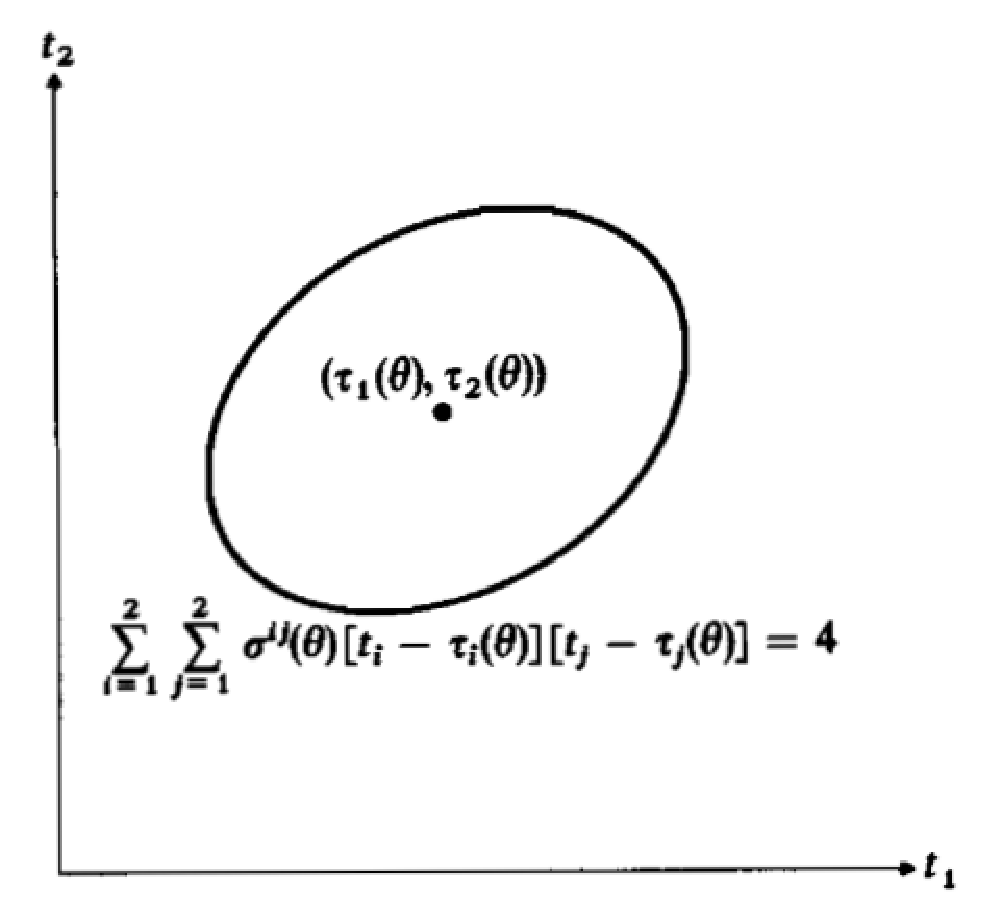
\includegraphics[scale = 0.5]{pictures/ellipsoid_of_concentration.eps}
\caption{Elipsoid koncentrace pro $r = 2$}
\label{ellipsoid-of-concentration}
\end{figure}

Elipsoid koncentrace tedy měří, jak je $(T_1, ..., T_r)$ ``koncentrováno'' okolo $(\tau_1(\theta), ..., \theta_r(\theta))$. Funkce odhadu $(T_1, ..., T_r)$, jejíž elipsoid koncentrace je obsažen v elipsoidu koncentrace jiné funkce odhadu $(T_1', ..., T_r')$, je více ``koncentrován'' okolo $\tau_1(\theta), ..., \tau_r(\theta)$ než $(T_1', ..., T_r')$.

Determinant kovarianční matice funkce odhadu je proporcionální čtverci plochy odpovídajícímu elipsoidu koncentrace. Tímto se dostáváme k Wilksově zobecnění rozptylu.

\begin{definition}[Wilksovo zobecnění rozptylu]
Uvažujme nezkreslenou funkci odhadu $(T_1, ..., T_r)$ pro $(\tau_1(\theta), ..., \tau_r(\theta))$. Wilkosův zobecněný rozptyl funkce odhadu $(T_1, ..., T_r)$ je definován jako determinant její kovarianční matice.
\end{definition}

Následující věta představuje zobecnění věty (7.9) pro $r$ dimenzí. Tuto větu uvádíme bez důkazu.
\begin{theorem}
Uvažujme náhodný výběr $X_1, ..., X_n$ z populace $f(x; \theta_1, ..., \theta_k)$. Nechť $S_1 = \mathfrak{s}_1(X_1, ..., X_n), ..., S_m = \mathfrak{s}_m(X_1, ..., X_n)$ jsou sdruženě dostatečné statistiky a nechť $(T_1, ..., T_r)$ představuje nezkreslenou funkci odhadu pro $(\tau_1(\theta), ..., \tau_r(\theta))$. Definujme $T_j' = E[T_j|S_1, ..., S_m]$ pro $j = 1, ..., r$. Pak
\begin{enumerate}
\item $(T_1', ..., T_r')$ je statistika a nezkreslená funkce odhadu pro $(\tau_1(\theta), ..., \tau_r(\theta))$ a $T_j' = \mathfrak{t}_j'(S_1, ..., S_m)$, tj. $T_j'$ je funkcí sdruženě dostatečných statistik $S_1, ..., S_m$.
\item $D_{\theta}[T_j'] \le D_{\theta}[T_j]$ pro každé $\theta \in \overline{\underline{\Theta}}$.
\item Elipsoid koncentrace pro $(T_1', ..., T_r')$ je obsažen v elipsoidu koncentrace pro $(T_1, ..., T_r)$ pro každé $\theta \in \overline{\underline{\Theta}}$.
\end{enumerate}
\end{theorem}

Bod (2) implikuje
\begin{equation*}
\sum_{j = 1}^r a_j D_{\theta}[T_j'] \le \sum_{j = 1}^r a_j D_{\theta}[T_j] ~~~\textit{pro}~ a_j \le 0
\end{equation*}
a bod (3) implikuje, že Wilksův zobecněný rozptyl pro $(T_1', ..., T_r')$ je menší než Wilksův zobecněný rozptyl pro $(T_1, ..., T_r)$.

Větu (7.11) lze taktéž zobecnit pro $r$ dimenzí. Nejprve je však třeba zobecnit koncept úplnosti.

\begin{definition}[Sdružená kompletnost]
Uvažujme náhodný výběr $X_1, ..., X_n$ z populace $f(x; \theta_1, ..., \theta_k)$. Nechť $(T_1, ..., T_m)$ představuje soubor statistik. Statistiky $T_1, ..., T_m$ nazýváme sdruženě kompletní, jestliže $E_{\theta}[\mathit{z}(T_1, ..., T_m)] \equiv 0$ pro všechna $\theta \in \overline{\underline{\Theta}}$ implikuje $P_{\theta}[\mathit{z}(T_1, ..., T_m) = 0] \equiv 1$ pro všechna $\theta \in \overline{\underline{\Theta}}$, kde $\mathit{z}(T_1, ..., T_m)$ je statistikou.
\end{definition}

\begin{example}
Uvažujme náhodný výběr z poulace $f(x; \theta_1, \theta_2) = \frac{1}{\theta_2 - \theta_1}I_{(\theta_1, \theta_2)}(x)$, kde $\theta_1 < \theta_2$. Definujme $\theta = (\theta_1, \theta_2)$, $Y_1 = \min(X_1, ..., X_n)$ a $Y_n = \max(X_1, ..., X_n)$. Pokusme se dokázat, že $X_1$ a $X_n$ jsou sdruženě kompletní\footnote{Z předchozího textu již víme, že jsou sdruženě dostatečné.}.

Uvažujme nezkreslenou funkci odhadu $\mathit{z}(Y_1, Y_n)$ pro 0, tj.
\begin{equation*}
E_{\theta}[\mathit{z}(Y_1, ..., Y_n)] \equiv 0 ~~~ \textit{pro všechna}~\theta \in \Theta
\end{equation*}
Dále
\begin{gather*}
E_{\theta}[\mathit{z}(Y_1, Y_n)] = \int \int \mathit{z}(y_1, y_n)f_{Y_1, Y_n}(y_1, y_n)d y_1 d y_n\\
= \int_{\theta_1}^{\theta_2}\left(\int_{\theta_1}^{y_n}\mathit{z}(y_1, y_n) n(n - 1)\left(\frac{y_n - \theta_1}{\theta_2 - \theta_1} - \frac{y_1 - \theta_1}{\theta_2 - \theta_1}\right)^{n - 2} \frac{1}{\theta_2 - \theta_1}\frac{1}{\theta_2 - \theta_1}dy_1\right)dy_n
\end{gather*}
což je shodou okolností rovno nule jen tehdy, jestliže
\begin{equation*}
\int_{\theta_1}^{\theta_2} \int_{\theta_1}^{y_n} \mathit{z}(y_1, y_n)(y_n - y_1)^{n - 2}dy_1 dy_n \equiv 0 ~~~ \textit{pro}~\theta_1 < \theta_2
\end{equation*}
Derivací obou stran vzhledem k $\theta_2$ získáme
\begin{equation*}
\int_{\theta_1}^{\theta_2} \mathit{z}(y_1, \theta_2)(\theta_2 - y_1)^{n - 2}dy_1 \equiv 0 ~~~ \textit{pro všechna}~\theta_1 < \theta_2
\end{equation*}
Následnou derivací dle $\theta_1$ získáme
\begin{equation*}
-\mathit{z}(\theta_1, \theta_2)(\theta_2 - \theta_1)^{n-2} \equiv 0 ~~~\textit{pro všechna}~\theta_1 < \theta_2
\end{equation*}
a proto $\mathit{z}(\theta_1, \theta_2) = 0$ pro $\theta_1 < \theta_2$, tj. $\mathit{z}(\theta_1, \theta_2) = 0$ pro $y_1 < y_n$. $Y_1$ a $Y_n$ jsou tak sdruženě kompletní.
\end{example}

Jestliže je $f(x; \theta_1, ..., \theta_k)$ je členem $k$-parametrické rodiny exponenciálních rozdělení, pak lze soubor sdruženě kompletních a dostatečných statistik nalézt s pomocí následující věty. Tato věta, kterou uvádíme bez důkazu, je zobecněním věty (7.10). Navíc jsou opomenuty některé podmínky regularity, a proto není zcela přesně formulována.

\begin{theorem}
Uvažujme náhodný výběr z populace $f(x; \theta_1, ..., \theta_k)$. Jestliže je  $f(x; \theta_1, ..., \theta_k)$ členem $k$-parametrické rodiny exponenciálních rozdělení, tj.
\begin{equation*}
f(x; \theta_1, ..., \theta_k) = a(\theta_1, ..., \theta_k)b(x)e^{\sum_{j = 1}^k c_j(\theta_1, ..., \theta_k)d_j(x)}
\end{equation*}
pak $\left(\sum d_1(X_i), ..., \sum d_k(X_i)\right)$ představuje soubor minimálních sdruženě kompletních a dostatečných statistik.
\end{theorem}

\begin{example}
Uvažujme náhodný výběr $X_1, ..., X_n$ z populace
\begin{equation*}
f(x; \theta_1, \theta_2) = \phi_{\theta_1, \theta_2^2}(x) = \frac{1}{\sqrt{2 \pi}\theta_2}e^{-\frac{1}{2}\left(\frac{x - \theta_1}{\theta_2}\right)^2}
\end{equation*}
Výše uvedenou pravděpodobnostní funkci lze také vyjádřit jako
\begin{equation*}
f(x; \theta_1, \theta_2) = \frac{1}{\sqrt{2 \pi} \theta_2}e^{-\frac{1}{2}\left(\frac{\theta_1}{\theta_2}\right)^2}e^{-\frac{x^2}{2 \theta_2^2} + \frac{\theta_1 x}{\theta_2^2}}
\end{equation*}
a proto jsou, dle výše uvedené věty, $\sum X_i$ a $\sum X_i^2$ sdruženě kompletní a dostatečné statistiky.
\end{example}

Následující věta je vektorovou analogií věty (7.11). Jestliže definujeme UMVUE jako optimum, pak lze s pomocí následující věty identifikovat optimální funkci odhadu pro vektor funkcí parametrů.

\begin{theorem}
Uvažujme náhodný výběr $X_1, ..., X_n$ z populace $f(x; \theta_1, ..., \theta_k)$. Definujme $\theta = (\theta_1, ..., \theta_k)$. Jestliže $S_1 = \mathfrak{s}_1(X_1, ..., X_n), ..., S_m = \mathfrak{s}_m(X_1, ..., X_n)$ jsou sdruženě kompletní a dostatečné statistiky a jestliže existuje nezkreslená funkce odhadu pro $(\tau_1(\theta), ..., \tau_r(\theta))$, pak existuje jedinečná nezkreslená funkce odhadu $T_1^* = \mathfrak{t}_1^*(S_1, ..., S_m), ..., T_r^* = \mathfrak{t}_r^*(S_1, ..., S_m)$ pro $(\tau_1(\theta), ..., \tau_r(\theta))$, která splňuje
\begin{itemize}
\item $D_{\theta}[T_j^*] \le D_{\theta}[T_j]$ pro každé $\theta \in \overline{\underline{\Theta}}$, $j = 1, ..., r$ a libovolnou alternativní funkci odhadu $(T_1, ..., T_r)$ pro $(\tau_1(\theta), ..., \tau_r(\theta))$,
\item Elipsoid koncentrace pro $(T_1^*, ..., T_r^*)$ je obsažen v elipsoidu koncentrace pro $(T_1, ..., T_r)$, kde $(T_1, ..., T_r)$ je libovolná alternativní nezkreslená funkce odhadu pro $(\tau_1(\theta), ..., \tau_r(\theta))$.
\end{itemize}
\end{theorem}

Funkci odhadu $(T_1^*, ..., T_r^*)$ lze nalézt dvěma způsoby. Prvním je kvalifikovaný odhad $\mathfrak{t}_1^*, ..., \mathfrak{t}_r^*$, které představují funkce sdruženě kompletních a dostatečných statistik $S_1, ..., S_m$ a které budou nezkreslenými funkcemi odhadu pro $(\tau_1(\theta), ..., \tau_r(\theta))$. Druhým způsobem je nalezení libovolného souboru nezkreslených funkcí odhadu pro $(\tau_1(\theta), ..., \tau_r(\theta))$ a následný výpočet jejich podmíněné střední hodnoty pro daný soubor sdruženě kompletních a dostatečných statistik $S_1, ..., S_m$.

\begin{example}
Uvažujme náhodný výběr z populace $f(x; \theta_1, \theta_2) = \frac{1}{\theta_2 - \theta_1}I_{(\theta_1, \theta_2)}(x)$. Pokusme se ``sdruženě'' odhadnout $\tau_1(\theta) = \theta_2 - \theta_1$ a $\tau_2(\theta) = \frac{\theta_1 + \theta_2}{2}$.

Z předchozího textu víme, že $Y_1 = \min(X_1, ..., X_n)$ a $Y_n = \max(X_1, ..., X_n)$ jsou sdruženě kompletní a dostatečné statistiky. Abychom tak našli nezkreslenou funkci odhadu $(T_1^*, T_2^*)$ s uniformě nejmenším rozptylem, stačí nalézt nezkreslenou funkci odhadu, která je funkcí těchto statistik. Protože $E[Y_1] = \theta_1 + \frac{\theta_2 - \theta_1}{n + 1}$ a $E[Y_n] = \theta_2 - \frac{\theta_2 - \theta_1}{n + 1}$, představuje $\left(\frac{n + 1}{n - 1}(Y_n - Y_1), \frac{Y_1 + Y_n}{2}\right)$ námi hledanou nezkreslenou funkci odhadu pro $\left(\theta_2 - \theta_1, \frac{\theta_1 + \theta_2}{2}\right)$.
\end{example}

\begin{example}
Uvažujme náhodný výběr $X_1, ..., X_n$ z normálního rozdělení $f(x; \theta_1, \theta_2) = \phi_{\mu, \sigma^2}(x)$. Z předchozího textu víme, že $\sum X_i$ a $\sum X_i^2$ jsou sdruženě kompletní a dostatečné statistiky. Proto na základě věty (7.20) je $\left(\sum \frac{X_i}{n}, \sum \frac{(X_i - \overline{X})^2}{n - 1}\right)$ nezkreslenou funkcí odhadu pro $(\mu, \sigma^2)$ jejíž elipsoid koncentrace je obsažen v elipsoidu koncentrace libovolné alternativní funkce odhadu\footnote{Protože $\sum(X_i - \overline{X})^2 = \sum X_i^2 - n \overline{X}^2$, je funkce odhadu $\frac{\sum (X_i - \overline{X})^2}{n - 1}$ funkcí sdruženě kompletních a dostatečných statistik $\sum X_i$ a $\sum X_i^2$.}.

Nyní předpokládejme, že chceme získat funkci odhadu pro $\theta = (\mu, \sigma^2)$ při splnění podmínky
\begin{equation*}
\int_{\tau(\theta)}^{\infty}\phi_{\mu, \sigma^2}(x)dx = \alpha
\end{equation*}
pro známé a fixní $\alpha$. $\tau(\theta)$ je $(1 - \alpha)$-tý kvantil, tj. splňuje podmínku $P[X_i > \tau(\theta)] = \alpha$. To implikuje $1 - \alpha = \Phi\left(\frac{\tau(\theta) - \mu}{\sigma}\right)$ neboli $\tau(\theta) = \mu + z_{1 - \alpha}\sigma$, kde $z_{1 - \alpha}$ je definováno vztahem $\Phi(z_{1 - \alpha}) = 1 - \alpha$. Abychom našli UMVUE pro $\tau(\theta)$, stačí nalézt nezkreslenou funkci odhadu pro $\mu + z_{1 - \alpha}\sigma$, která je sama funkcí $\sum X_i$ a $\sum X_i^2$. Protože $\overline{X}$ je UMVUE pro $\mu$ a protože lze dokázat, že
\begin{equation*}
\frac{\Gamma\left(\frac{n - 1}{2}\right)}{\Gamma \left(\frac{n}{2}\right) \sqrt{2}}\sqrt{\sum_{i = 1}^n(X_i - \overline{X})^2} = T^*
\end{equation*}
je UMVUE pro $\sigma$, je $\overline{X} + z_{1 - \alpha}T^*$ UMVUE pro $\tau(\theta)$. Při odvození jsme aplikovali větu (7.20) pro $r = 1$.
\end{example}

\section{Odhad maximální věrohodnosti}

Uvažujme náhodný výběr $X_1, ..., X_n$ z populace $f(\cdot, \theta)$, kde $\theta$ je reálné číslo. Pro pozorované hodnoty $x_1, ..., x_n$ je odhad $\hat{\theta}$ parametru $\theta$ dán maximem funkce věrohodnosti
\begin{equation*}
L(\theta; x_1, ..., x_n) = \prod_{i = 1}^n f(x_i, \theta)
\end{equation*}
Označme funkci odhadu založenou na principu maximální věrohodnosti jako $\hat{\Theta}_n = \hat{\zeta}_n(X_1, ..., X_n)$. Z předchozího textu víme, že je žádoucí, aby funkce odhadu splňovala některé podmínky.
\begin{theorem}
Uvažujme náhodný výběr $X_1, ..., X_n$ z populace $f(x, \theta)$, kde $f(x, \theta)$ splňuje určité podmínky regularity. Je-li $\hat{\Theta} = \hat{\zeta}_n(X_1, ..., X_n)$ funkcí odhadu dle maximální věrohodnosti pro $\theta$, pak
\begin{enumerate}
\item $\hat{\Theta}_n$ je asymptoticky normálně rozdělené se střední hodnotou $\theta$ a rozptylem $\frac{1}{n}E\left[\left(\frac{\partial}{\partial \theta} \ln(f(X, \theta))\right)^2\right]$,
\item posloupnost funkcí odhadu $\hat{\Theta}_1, ..., \hat{\Theta}_n$ je BAN.
\end{enumerate}
\end{theorem}

Výše uvedená věta, kterou nebudeme dokazovat, říká, že pro náhodné výběry velkého rozsahu je funkce odhadu pro $\theta$ založená na metodě maximální věrohodnosti nejlepší možnou funkcí odhadu\footnote{Mohou existovat jiné funkce odhadu, které budou stejně dobré ale ne lepší.}. Dále platí, že rozptyl asymptotického normálního rozdělení v bodě (1) je Cramér-Raovou dolní mezí rozptylu.

\begin{example}
Uvažujme náhodný výběr $X_1, ..., X_2$ z negativního exponenciálního rozdělení $f(x, \theta) = \theta e^{-\theta x}I_{[0, \infty)}(x)$. Lze odvodit, že funkce odhadu dle maximální věrohodnosti pro $\theta$ je $\frac{\sum X_i}{n} = \frac{1}{\overline{X}}$. Dle výše uvedené věty má tato funkce odhadu asymptoticky normální rozdělení se střední hodnotou $\theta$ a rozptylem\footnote{Viz. příklad (7.31)}
\begin{equation*}
\frac{1}{n E_{\theta}\left[\left(\frac{\partial}{\partial \theta}\ln(f(X, \theta))\right)\right]} = \frac{\theta^2}{n}
\end{equation*}
\end{example}

Dle věty (7.2) je funkce odhadu pro $\tau(\theta)$ daná metodou maximální věrohodnosti $\tau(\hat{\Theta})$. Jestliže má $\tau(\cdot)$ derivaci prvního stupně, lze dokázat, že $\tau(\hat{\Theta})$ má asymptoticky normální rozdělení se střední hodnotou $\tau(\theta)$ a rozptylem
\begin{equation*}
\frac{[\tau'(\theta)]^2}{n E_{\theta}\left[\left(\frac{\partial}{\partial \theta}\ln(f(X, \theta))\right)^2\right]}
\end{equation*}
který představuje Cramér-Raovu dolní mez rozptylu.

Funkce odhadu dle metody maximální věrohodnosti si zachovává výše uvedené vlastnosti také v případě, kdy je $\theta$ $k$-rozměrným vektorem. Lze totiž opět dokázat, že při splnění určitých podmínek regularity, lze funkce odhadu popsat pomocí asymptotického vícerozměrného normálního rozdělení. Je-li např. $k = 2$, tj. $\theta = (\theta_1, \theta_2)$, sledují $\hat{\Theta}_1$ a $\hat{\Theta}_2$ asymptoticky dvourozměrné normální rozdělení s parametry
\begin{gather*}
\mu_1 = \theta_1\\
\sigma_1^2 = - \frac{E_{\theta}\left[\frac{\partial^2}{\partial \theta_2^2}\ln(f(X, \theta))\right]}{n \Delta}\\
\mu_2 = \theta_2\\
\sigma_2^2 = - \frac{E_{\theta}\left[\frac{\partial^2}{\partial \theta_1^2}\ln(f(X, \theta))\right]}{n \Delta}\\
\rho_{\sigma_1, \sigma_2} = \frac{E_{\theta}\left[\frac{\partial^2}{\partial \theta_2 \theta_1}\ln(f(X, \theta))\right]}{n \Delta}
\end{gather*}
kde
\begin{equation*}
\Delta = E_{\theta}\left[\frac{\partial^2}{\partial \theta_1^2}\ln(f(X, \theta))\right]E_{\theta}\left[\frac{\partial^2}{\partial \theta_2^2}\ln(f(X, \theta))\right] - \left(E_{\theta}\left[\frac{\partial^2}{\partial \theta_1 \theta_2}\ln(f(X, \theta))\right]\right)^2
\end{equation*}

\begin{example}
Uvažujme náhodný výběr z populace
\begin{equation*}
f(x, \theta) = f(x; \theta_1, \theta_2) = \phi_{\theta_1, \theta_2}(x) = \frac{1}{\sqrt{2 \pi \theta_2}}e^{-\frac{1}{2 \theta_2}(x - \theta_1)^2}
\end{equation*}
V předchozích příkladech jsme odvodily funkce odhadu dle metody maximální věrohodnosti pro $\theta_1$ a $\theta_2$.
\begin{gather*}
\hat{\Theta}_1 = \frac{1}{n}\sum_{i = 1}^n X_i\\
\hat{\Theta}_2 = \frac{1}{n}\sum_{i = 1}^n (X_i - \hat{\Theta}_1)^2
\end{gather*}
Asymptotické dvourozměrné normální rozdělení $\hat{\Theta}_1$ a $\hat{\Theta}_2$ má střední hodnoty $\theta_1$ a $\theta_2$. Protože $\ln(f(X, \theta)) = -\frac{1}{2}\ln(\theta_2) - \frac{1}{2 \theta_2}(X - \theta_1)^2$, jsou hledané derivace
\begin{gather*}
\frac{\partial^2}{\partial \theta_1^2} \ln(f(X, \theta)) = -\frac{1}{\theta_2}\\
\frac{\partial^2}{\partial \theta_2 \theta_1} \ln(f(X, \theta)) = -\frac{X - \theta_1}{\theta_2^2}\\
\frac{\partial^2}{\partial \theta_2^2} \ln(f(X, \theta)) = \frac{1}{2 \theta_2^2} -\frac{(X - \theta_1)^2}{\theta_2^3}\\
\end{gather*}
Platí
\begin{gather*}
E[X] = \theta_1\\
E[(X - \theta_1)^2] = \theta_2\\
-E_{\theta}\left[\frac{\partial^2}{\partial \theta_1^2} \ln(f(X, \theta))\right] = \frac{1}{\theta_2}\\
-E_{\theta}\left[\frac{\partial^2}{\partial \theta_2 \partial \theta_1}\ln(f(X, \theta))\right] = 0\\
-E_{\theta}\left[\frac{\partial^2}{\partial \theta_2^2} \ln(f(X, \theta))\right] = \frac{1}{2\theta_2^2}\\
\end{gather*}
což implikuje $\Delta = \frac{1}{2 \theta_2^2}$. Zbývající parametry dvourozměrného normálního rozdělení tak jsou $\sigma_1^2 = \frac{\theta_2}{n}, \sigma_2^2 = \frac{2 \theta_2^2}{n}$ a $\rho = 0$.
\end{example}



\chapter{Intervalový odhad}

\section{Interval spolehlivosti}

\subsection{Definice intervalu spolehlivosti}

\begin{definition}[Interval spolehlivosti]
Uvažujme náhodný výběr $X_1, ..., X_n$ z populace $f(\cdot, \theta)$. Nechť $T_1 = \mathfrak{t}_1(X_1, ..., X_n)$ a $T_2 = \mathfrak{t}_2(X_1, ..., X_n)$ představují dvě statistiky, které splňují podmínku $T_1 \le T_2$ a pro které platí $P_{\theta}[T_1 < \tau(\theta) < T_2] \equiv \gamma$, kde $\gamma$ není funkcí $\theta$. Náhodný interval $(T_1, T_2)$ nazýváme 100$\gamma$ procentním intervalem spolehlivosti pro $\tau(\theta)$ a $T_1$ resp. $T_2$ nazýváme jeho dolním resp. horním limitem. Hodnotu  $(t_1, t_2)$ náhodného intervalu $(T_1, T_2)$ taktéž nazýváme 100$\gamma$ procentním intervalem spolehlivosti pro $\tau(\theta)$.
\end{definition}

Jedna ze statistik $\mathfrak{t}_1(X_1, ..., X_n)$ a $\mathfrak{t}_2(X_1, ..., X_n)$ může být konstantou.

\begin{definition}[Jednostranný interval spolehlivosti]
Uvažujme náhodný výběr $X_1, ..., X_n$ z populace $f(\cdot, \theta)$. Nechť $T_1 = \mathfrak{t}_1(X_1, ..., X_n)$ je statistika, pro kterou platí $P_{\theta}[T_1 < \tau(\theta)] \equiv \gamma$. Pak $T_1$ nazýváme levostranným limitem spolehlivosti pro $\tau(\theta)$. Podobně, je-li $T_2 = \mathfrak{t}_2(X_1, ..., X_n)$ statistika, pro kterou platí $P_{\theta}[\tau(\theta) < T_2]$, pak nazýváme $T_2$ pravostranným intervalem spolehlivosti pro $\tau(\theta)$.
\end{definition}

\begin{example}
Uvažujme náhodný výběr z populace $f(x, \theta) = \phi_{0, 9}(x)$. Definujme $T_1 = \mathfrak{t}_1(X_1, ..., X_n) = \overline{X} - \frac{6}{\sqrt{n}}$ a $T_2 = \mathfrak{t}_2(X_1, ..., X_n) = \overline{X} + \frac{6}{\sqrt{n}}$. Pak $(T_1, T_2)$ představuje interval spolehlivosti pro $\tau(\theta) = \theta$ s koeficientem spolehlivosti $\gamma = P_{\theta}[\overline{X} - \frac{6}{\sqrt{n}} < \theta < \overline{X} + \frac{6}{\sqrt{n}}] = P_{\theta}[-2 < \frac{\overline{X} - \theta}{3 / \sqrt{n}} < 2] = \Phi(2) - \Phi(-2) = 0.9772 - 0.0228 = 0.9544$. Jestliže by střední hodnota náhodného výběru o, řekněme, 25 prvcích byla 17.5, pak je interval $(17.5 - \frac{6}{\sqrt{25}}, 17.5 + \frac{6}{\sqrt{25}})$ nazýván 95.44 procentním intervalem spolehlivosti pro $\theta$.
\end{example}

Z daného 100$\gamma$ procentního intervalu spolehlivosti pro $\theta$ je možné odvodit 100$\gamma$ procentní interval spolehlivosti pro $\tau(\theta)$ za předpokladu, že $\tau(\cdot)$ je striktně monotonní funkcí. Jestliže je $\tau(\cdot)$ rostoucí funkcí a $(T_1, T_2)$ je 100$\gamma$ procentním intervalem spolehlivosti pro $\theta$, pak $(\tau(T_1), \tau(T_2))$ je 100$\gamma$ procentním intervalem spolehlivosti pro $\tau(\theta)$, protože
\begin{equation*}
P_{\theta}[\tau(T_1) < \tau(\theta) < \tau(T_2)] = P_{\theta}[T_1 < \theta < T_2]
\end{equation*}

Stejně jako v případě bodového odhadu čelíme dvojímu problému. Prvním problémem je definování metod pro nalezení intervalu spolehlivosti. Druhým problémem je nalezení vhodného kritéria pro porovnání všech možných intervalů spolehlivosti. Tímto se dostáváme k následující kapitole.

\subsection{Centrální veličina}

\begin{definition}[Centrální veličina]
Uvažujme náhodný výběr $X_1, ..., X_n$ z populace $f(x, \theta)$. Definujme $Q = \mathit{q}(X_1, ..., X_n; \theta)$. Jestliže pravděpodobnostní funkce náhodné veličiny $Q$ nezávisí na $\theta$, pak ji nazýváme centrální veličinou.
\end{definition}

\begin{example}
Uvažujme náhodný výběr $X_1, ..., X_n$ z populace $f(x, \theta) = \phi_{\theta, 9}(x)$. $\overline{X} - \theta$ je centrální veličinou, protože $\overline{X} - \theta$ sleduje normální rozdělení se střední hodnotou nula a rozptylem $9/n$. Také $\frac{\overline{X} - \theta}{3/ \sqrt{n}}$ je centrální veličinou, protože sleduje normalizované normální rozdělení. Naproti tomu $\overline{X}/ \theta$ není centrální veličinou, protože sleduje normální rozdělení s jednotkovou střední hodnotou a rozptylem $9/\theta^2n$.
\end{example}

\begin{definition}[Metoda centrální veličiny]
Jestliže $Q = \mathit{q}(X_1, ..., X_n; \theta)$ je centrální veličinou, pak pro libovolné $0 < \gamma < 1$ existují $q_1$ a $q_2$ taková, že $P[q_1 < Q < q_2] = \gamma$. Jestliže pro libovolné realizace náhodného výběru $x_1, ..., x_n$ platí $q_1 < \mathit{q}(x_1, ..., x_n; \theta) < q_2$ tehdy a jen tehdy, jestliže $\mathfrak{t}_1(x_1, ..., x_n) < \tau(\theta) < \mathfrak{t}_2(x_1, ..., x_n)$\footnote{Připomeňme, že funkce $\mathit(t)_1$ a $\mathit(t)_2$ nezávisí na $\theta$.}, pak $(T_1, T_2)$ představuje 100$\gamma$ procentní interval spolehlivosti pro $\tau(\theta)$, kde $T_i = \mathfrak{t}_i(X_1, ..., X_n)$ pro $i = 1, 2$.
\end{definition}

Je zřejmé, že $q_1$ a $q_2$ jsou nezávislé na $\theta$, protože $Q$ je taktéž nezávislé na $\theta$.

Pro každou hodnotu $\gamma$ existuje mnoho možných párů $q_1$ a $q_2$, které splňují podmínku $P[q_1 < Q < q_2] = \gamma$. Různá $q_1$ a $q_2$ definují různé funkce $\mathfrak{t}_1$ a $\mathfrak{t}_2$. Je zřejmé, že preferujeme taková $\mathfrak{t}_1$ a $\mathfrak{t}_2$, která jsou si pokud možno co ``nejblíže''. Definujme tuto ``blízkost'' jako $\mathfrak{t}_2(X_1, ..., X_n) - \mathfrak{t}_1(X_1, ..., X_n)$. Jestliže vzdálenost mezi $\mathfrak{t}_1$ a $\mathfrak{t}_2$ nemá charakter náhodné veličiny, pak vybereme taková $q_1$ a $q_2$, která tuto vzdálenost minimalizují. Pokud má tato vzdálenost charakter náhodné veličiny, pak vybereme taková $q_1$ a $q_2$, která minimalizují její střední hodnotu.

Základním požadavkem na centrální veličinu je, že nerovnost $\{q_1 < \mathit{q}(x_1, ..., x_n; \theta) < q_2\}$ lze přepsat do tvaru $\{\mathfrak{t}_1(x_1, ..., x_n) < \tau(\theta) < \mathfrak{t}_2(x_1, ..., x_n)\}$ pro libovolnou realizaci náhodného výběru $x_1, ..., x_n$. Tato vlastnost však není implikována výše uvedenou definici centrální veličiny.

\begin{example}
Uvažujme náhodný výběr $X_1, ..., X_n$ z $\phi_{\theta, 1}$. Nechť $\tau(\theta) = \theta$. Náhodná veličina $Q = \mathit{q}(X_1, ..., X_n; \theta) = \frac{\overline{X} - \theta}{\sqrt{1}{n}}$ sleduje normalizované normální rozdělení, a proto představuje centrální veličinu. Platí $f_Q(q) = \phi(q)$. Pro dané $0 < \gamma < 1$ existuje nekonečně párů $q_1$ a $q_2$, které splňují podmínku $P[q_1 < Q < q_2] = \gamma$.

$\{q_1 < \frac{\overline{x} - \theta}{\sqrt{1/n}} < q_2\}$ implikuje $\{\overline{x} - q_2\sqrt{1/n} < \theta < \overline{x} - q_1 \sqrt{1/n}\}$. Proto je interval  $\{\overline{X} - q_2\sqrt{1/n} < \theta < \overline{X} - q_1 \sqrt{1/n}\}$ 100$\gamma$ procentním intervalem spolehlivosti pro $\theta$. Délka tohoto intervalu je $(\overline{X} - q_1\sqrt{1/n}) - (\overline{X} - q_2 \sqrt{1/n}) = (q_2 - q_1)\sqrt{1/n}$ a je proto nejkratší pro nejmenší hodnotu $q_2 - q_1$ při splnění podmínky $\gamma = P[q_1 < Q < q_2] = \Phi(q_2) - \Phi(q_1)$. Délka tohoto intervalu tak dosahuje minima pro $q_1 = - q_2$.
\end{example}

\section{Náhodný výběr z normálního rozdělení}

\subsection{Interval spolehlivosti pro střední hodnotu}

Uvažujme náhodný výběr $X_1, ..., X_n$ z populace, která sleduje normální rozdělení, jejíž střední hodnotu ani rozptyl neznáme. To znamená, že $\theta = (\mu, \sigma)$ a $\tau(\theta) = \mu$. Náhodná veličina $\frac{\overline{X} - \mu}{\sigma / \sqrt{n}}$ sleduje normované normální rozdělení, a proto je centrální veličinou. Nicméně $\{q_1 < \frac{\overline{x} - \mu}{\sigma / \sqrt{n}} < q_2 \}$ nelze převést do tvaru $\{\mathfrak{t}_1(x_1, ..., x_n) < \mu < \mathfrak{t}_1(x_1, ..., x_n)\}$. Důvodem je, že $\frac{\overline{X} - \mu}{\sigma / \sqrt{n}}$ obsahuje neznámé $\sigma$. Připomeňme, že hledáme centrální veličinu, jejíž jedinou neznámou je $\mu$. Nicméně víme, že
\begin{equation*}
\frac{\frac{\overline{X} - \mu}{\frac{\sigma}{\sqrt{n}}}}{\sqrt\frac{\sum_{i = 1}^n (X_i - \overline{X})^2}{(n - 1)\sigma^2}} = \frac{\overline{X} - \mu}{S_n / \sqrt{n}}
\end{equation*}
sleduje studentovo rozdělení s $n - 1$ stupni volnosti\footnote{Připomeňme, že $S_n^2 = \frac{\sum_{i = 1}^2}{n - 1}$.}. Pravděpodobnostní funkce náhodné veličiny $\frac{\overline{X} - \mu}{S_n / \sqrt{n}}$ je tak nezávislá na $\mu$ a $\sigma^2$, a proto se jedná o centrální veličinu. Nerovnosti $\{q_1 < \frac{\overline{x} - \mu}{\mathit{s} / \sqrt{n}} < q_2\}$ implikují $\{\overline{x} - q_2\frac{\mathit{s}}{\sqrt{n}} < \mu < \overline{x} - q_1\frac{\mathit{s}}{\sqrt{n}}\}$, kde $q_1$ a $q_2$ splňují podmínku $P[q_1 < \frac{\overline{X} - \mu}{S_n / \sqrt{n}} < q_2] = \gamma$. Proto je $(\overline{X} - q_2 \frac{S_n}{\sqrt{n}}, (\overline{X} - q_1 \frac{S_n}{\sqrt{n}})$ 100$\gamma$ procentním intervalem spolehlivosti pro $\mu$. Délka tohoto intervalu je $\frac{q_2 - q_1}{S / \sqrt{n}}$, což je náhodná veličina. Pro libovolný náhodný výběr je jeho délka minimalizována pro nejmenší $q_2 - q_1$. To je splněno pro $q_1 = - q_2$, jak dokazuje následující text.

Naším cílem je minimalizovat
\begin{equation*}
L = \frac{S_n}{\sqrt{n}}(q_2 - q_1)
\end{equation*} 
při splnění podmínky
\begin{equation*}
\int_{q_1}^{q_2} f_T(t) dt = \gamma
\end{equation*}
kde $f_T(t)$ je pravděpodobnostní funkce studentova rozdělení s $n - 1$ stupni volnosti. Derivací výše uvedené rovnice podle $q_1$ získáme
\begin{equation*}
f_T(q_2)\frac{d q_2}{d q_1} - f_T(q_1) = 0
\end{equation*}
Abychom minimalizovali $L$, musíme řešit rovnici $\frac{dL}{d q_1}$, tj.
\begin{equation*}
\frac{dL}{dq_1} = \frac{S_n}{\sqrt{n}}\left(\frac{d q_2}{d q_1} - 1 \right) = 0
\end{equation*}
Zároveň však platí
\begin{equation*}
\frac{S_n}{\sqrt{n}}\left(\frac{d q_2}{d q_1} - 1\right) = \frac{S_n}{\sqrt{n}}\left(\frac{f_t(q_1)}{f_t(q_2)} - 1\right) = 0
\end{equation*}
Tato rovnost je tedy splněna pro $f_T(q_2) = f_T(q_1)$, což v kontextu symetrického studentova rozdělení znamená $q_1 = - q_2$.

\subsection{Interval spolehlivosti pro rozptyl}

Uvažujme náhodný výběr $X_1, ..., X_n$ z populace, která sleduje normální rozdělení, jejíž střední hodnotu ani rozptyl neznáme. Víme, že náhodná veličina
\begin{equation*}
Q = \frac{\sum_{i = 1}^n (X_i - \overline{X})^2}{\sigma^2} = \frac{(n - 1)S_n^2}{\sigma^2}
\end{equation*}
sleduje chi-kvadrát rozdělení s $n - 1$ stupni volnosti. Náhodná veličina $Q$ je tedy centrální veličinou. Je zřejmé, že $\big\{q_1 < \frac{(n - 1)\mathit{s}^2}{\sigma^2} < q_2 \big\}$ implikuje $\big\{\frac{(n - 1) \mathit{s}^2}{q_2} < \sigma^2 < \frac{(n - 1)s^2}{q_1}\big\}$. To znamená, že $\left(\frac{(n - 1)S_n^2}{q_2}, \frac{(n - 1)S_n^2}{q_1} \right)$ je 100$\gamma$ procentní interval spolehlivosti pro $\sigma^2$, $q_1$ a $q_2$ splňují podmínku $P[q_1 < Q < q_2] = \gamma$.

$q_1$ a $q_2$ jsou často zvoleny tak, aby $P[Q < q_1] = P[Q > q_2] = \frac{1 - \gamma}{2}$. O takovémto intervalu spolehlivosti pak hovoříme jako o intervalu spolehlivosti se shodnými chvosty.

Další možností je nalézt taková $q_1$ a $q_2$, která minimalizují délku intervalu $L$, kde
\begin{equation*}
L = (n - 1)S_n^2 \left(\frac{1}{q_1} - \frac{1}{q_2}\right)
\end{equation*}
Nechť $f_Q(q)$ představuje pravděpodobnostní funkci chi-kvadrát rozdělení s $n - 1$ stupni volnosti. Derivací podmínky
\begin{equation*}
\int_{q_1}^{q_2} f_Q(q)dq = \gamma
\end{equation*}
dle $q_1$ získáváme
\begin{equation*}
\frac{dq_2}{dq_1}f_Q(q_2) - f_Q(q_1) = 0
\end{equation*}
a proto
\begin{equation*}
\frac{dL}{dq_1} = (n - 1)S_n^2\left(-\frac{1}{q_1^2} + \frac{1}{q_2^2}\frac{dq_2}{dq_1}\right) = (n - 1)S_n^2\left(- \frac{1}{q_1^2} + \frac{1}{q_2^2}\frac{f_Q(q_1)}{f_Q(q_2)}\right) = 0
\end{equation*}
což implikuje $q_1^2 f_Q(q_1) = q_2^2 f_Q(q_2)$. Délka intervalu spolehlivosti tak bude minimální pro $q_1$ a $q_2$ taková, že
\begin{equation*}
q_1^2 f_Q(q_1) = q_2^2 f_Q(q_2)
\end{equation*}
při splnění podmínky
\begin{equation*}
\int_{q_1}^{q_2} f_Q(q) dq = \gamma
\end{equation*}
Řešení pro $q_1$ a $q_2$ lze nalézt pomocí numerické integrace.

Závěrem uveďme, že pro libovolná $q_1$ a $q_2$ taková, že $\int_{q_1}^{q_2}f_Q(q)dq = \gamma$ představuje $\left(\sqrt{\frac{(n - 1)S_n^2}{q_2}}, \sqrt{\frac{(n - 1)S_n^2}{q_1}}
\right)$ 100$\gamma$ procentní interval spolehlivosti pro $\sigma$.

\subsection{Region spolehlivosti pro střední hodnotu a rozptyl}

Při konstrukci regionu spolehlivosti pro střední hodnotu $\mu$ a rozptyl $\sigma^2$ normálního rozdělení by se na první pohled mohlo zdát, že stačí rutinně aplikovat postup předešlých dvou kapitol. To znamená, že např. pro konstrukci 95 procentního regionu spolehlivosti ilustrovaného obrázkem (\ref{conf-interval-mu-sigma_a}) by stačilo použít vztahů
\begin{gather*}
P\left[\overline{X} - t_{0.975}\frac{S_n^2}{n} < \mu < \overline{X} + t_{0.975}\frac{S_n^2}{n}\right] = 0.95\\
P\left[\frac{(n - 1)S_n^2}{\chi_{0.975}^2} < \sigma^2 < \frac{(n - 1)S_n^2}{\chi_{0.025}^2}\right] = 0.95
\end{gather*}
kde $t_{0.975}$ představuje 97.5 procentní kvantil studentova rozdělení s $n - 1$ stupni volnosti a $\chi_{0.025}^2$ resp. $\chi_{0.975}^2$ představuje 2.5 resp. 97.5
 procentní kvantil chi-kvadrát rozdělení s $n - 1$ stupni volnosti. Region ilustrovaný obrázkem (\ref{conf-interval-mu-sigma_a}) je sice regionem spolehlivosti pro $(\mu, \sigma^2)$, ale jeho koeficient spolehlivosti neznáme. Víme pouze, že tento koeficient není $0.95^2$, protože výše uvedené dva vztahy nejsou nezávislé.

\begin{figure}[htp]
\centering
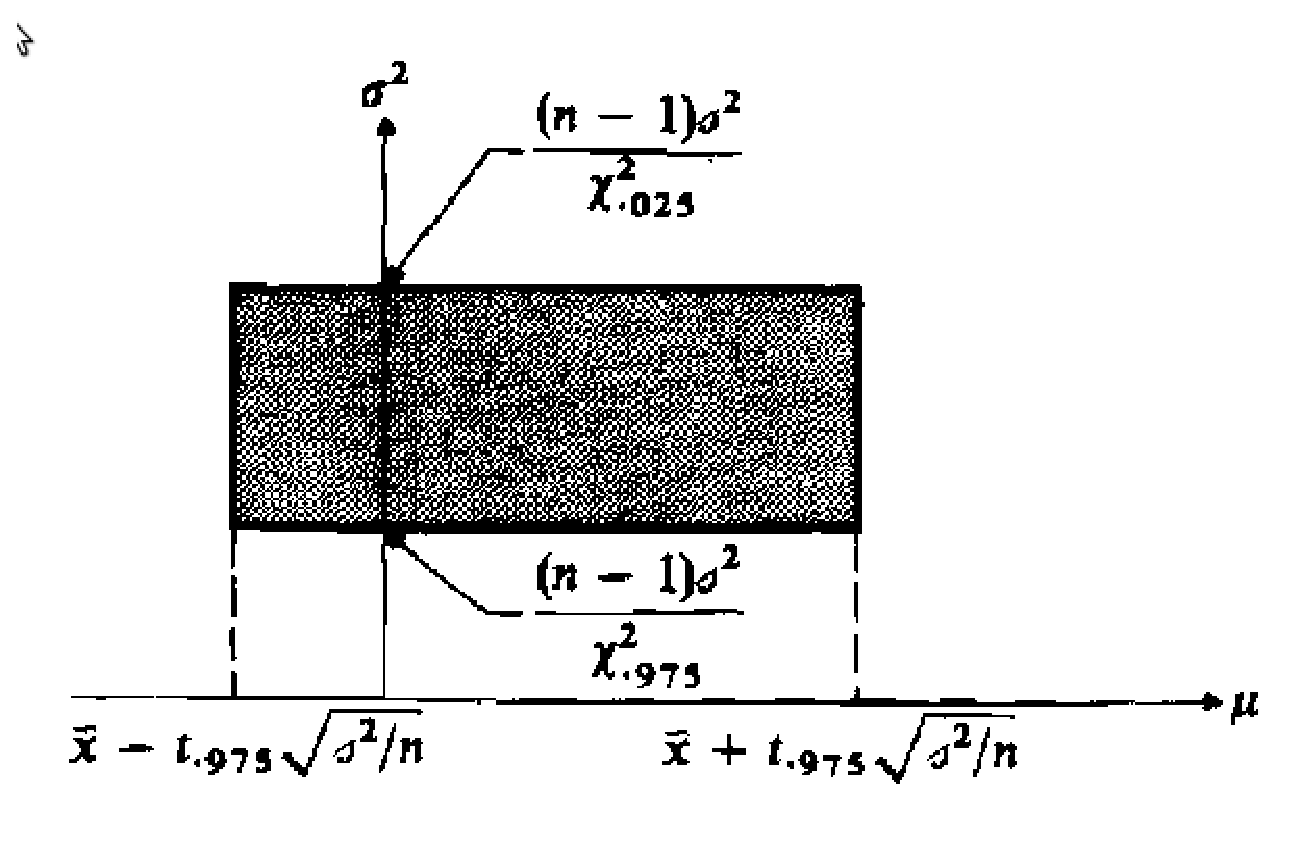
\includegraphics[scale = 0.5]{pictures/conf_interval_mu_sigma_a.eps}
\caption{Region spolehlivosti pro střední hodnotu a rozptyl}
\label{conf-interval-mu-sigma_a}
\end{figure}

Při stanovení regionu spolehlivosti je třeba vzít v potaz vzájemnou nezávislost $\overline{X}$ a $S_n^2$. Protože $Q_1 = \frac{\overline{X} - \mu}{\sigma / \sqrt{n}}$ a $Q_2 = \frac{(n - 1)S_n^2}{\sigma^2}$ představují centrální veličinu, lze nalézt $q_1, q_2'$ a $q_2''$ taková, že
\begin{gather*}
P \left[-q_1 < \frac{\overline{X} - \mu}{\sigma / \sqrt{n}} < q_1 \right] = \gamma_1\\
P \left[q_2' < \frac{(n - 1)S_n^2}{\sigma^2} < q_2'' \right] = \gamma_2
\end{gather*}
Protože jsou $Q_1$ a $Q_2$ vzájemně nezávislé, je jejich sdružená pravděpodobnost rovna
\begin{equation*}
P\left[-q_1 < \frac{\overline{X} - \mu}{\sigma / \sqrt{n}} < q_1, q_2' < \frac{(n - 1)S_n^2}{\sigma^2} < q_2'' \right] = \gamma_1 \gamma_2
\end{equation*}
Čtyři nerovnosti ve výše uvedeném výrazu určují region spolehlivosti, který ilustruje šedivá plocha obrázku (\ref{conf-interval-mu-sigma_b}).

\begin{figure}[htp]
\centering
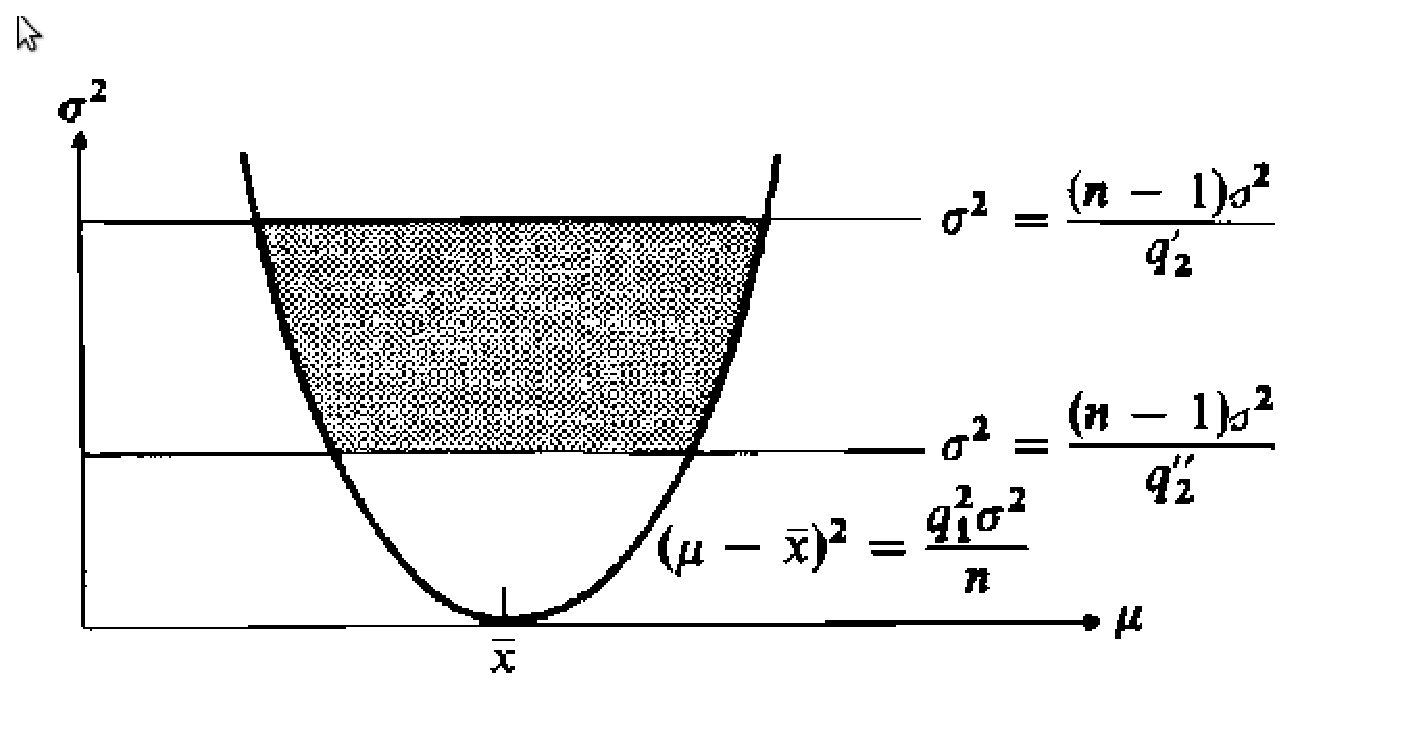
\includegraphics[scale = 0.5]{pictures/conf_interval_mu_sigma_b.eps}
\caption{Region spolehlivosti pro střední hodnotu a rozptyl}
\label{conf-interval-mu-sigma_b}
\end{figure}

Pro $(\mu, \sigma)$ bychom odvodili region spolehlivosti stejně jako v případě $(\mu, \sigma^2)$. Jediným rozdílem by bylo, že bychom pro osu $y$ použili $\sigma$ namísto $\sigma^2$ a parabola z obrázku (\ref{conf-interval-mu-sigma_b}) by se změnila na dvojici polopřímek daných rovnicemi $\mu = \overline{x} \pm q_1 \frac{\sigma}{\sqrt{n}}$, které se protínají v bodě $\overline{x}$ a ose $\mu$.

Závěrem je třeba zdůraznit, že region, který jsme zkonstruovali, nemá pro daná $\gamma_1$ a $\gamma_2$ minimální plochu. Výhoda výše popsaného postupu však spočívá v jeho jednoduchosti a ve skutečnosti, že pro přijatelně veliký náhodný výběr se takto získaný region spolehlivosti příliš neliší od minimálního regionu spolehlivosti. Minimální region spolehlivosti má přibližně eliptický tvar a jeho odvození je poměrně komplikované.

\subsection{Interval spolehlivosti pro rozdíl středních hodnot}

\subsubsection{Dva nezávislé náhodné výběry}

Uvažujme náhodný výběr $X_1, ..., X_m$ z normálního rozdělení se střední hodnotou $\mu_1$ a rozptylem $\sigma^2$ a náhodný výběr $Y_1, ..., Y_n$ z normálního rozdělení se střední hodnotou $\mu_2$ a rozptylem $\sigma^2$. Předpokládejme, že tyto dva náhodné výběry jsou vzájemně nezávislé. Pokusme se nalézt interval spolehlivosti pro $\mu_2 - \mu_1$.

Náhodná veličina $\overline{Y} - \overline{X}$ je normálně rozdělená se střední hodnotou $\mu_2 - \mu_1$ a rozptylem $\frac{\sigma^2}{n} + \frac{\sigma^2}{m}$. Náhodná veličina $\frac{\sum (X_i - \overline{X})^2}{\sigma^2}$ sleduje chi-kvadrát rozdělení s $m - 1$ stupni volnosti a náhodná veličina $\frac{\sum (Y_i - \overline{Y})^2}{\sigma^2}$ sleduje chi-kvadrát rozdělení s $n - 1$ stupni volnosti. Proto náhodná veličina $\frac{\sum (X_i - \overline{X})^2}{\sigma^2} + \frac{\sum (Y_i - \overline{Y})^2}{\sigma^2}$ sleduje chi-kvadrát rozdělení s $m + n - 2$ stupni volnosti. A konečně náhodná veličina
\begin{gather*}
Q = \frac{\frac{(\overline{Y} - \overline{X}) - (\mu_2 - \mu_1)}{\sqrt{\sigma^2/m + \sigma^2/n}}}{\sqrt{\frac{\sum_{i = 1}^n (X_i - \overline{X})^2 + \sum_{i = 1}^n(Y_i - \overline{Y})^2}{\sigma^2(m + n - 2)}}}\\
= \frac{(\overline{Y} - \overline{X}) - (\mu_2 - \mu_1)}{\sqrt{\left(\frac{1}{m} + \frac{1}{n} \right)\frac{\sum_{i = 1}^n(X_i - \overline{X})^2 + \sum_{i = 1}^n (Y_i - \overline{Y})^2}{m + n - 2}}}\\
= \frac{(\overline{Y} - \overline{X}) - (\mu_2 - \mu_1)}{\sqrt{\left(\frac{1}{m} + \frac{1}{n} \right)S_n^{'2}}}
\end{gather*}
sleduje studentovo rozdělení s $m + n - 2$ stupni volnosti. Z toho vyplývá $\gamma = P[-t_{(1 + \gamma) / 2} < Q < t_{(1 + \gamma) / 2}]$, kde $t_{(1 + \gamma) / 2}$ představuje $(1 + \gamma) / 2$ procentní kvantil studentova rozdělení s $m + n - 2$ stupni volnosti. $S_n^{'2}$ je nezkreslená funkce odhadu společného rozptylu $\sigma^2$. Dvojice nerovností
\begin{equation*}
- t_{(1 + \gamma) / 2} < \frac{(\overline{y} - \overline{x}) - (\mu_2 - \mu_1)}{\sqrt{(1/m + 1/n)\mathit{s}^{'2}}} < t_{(1 + \gamma)/2}
\end{equation*}
implikuje
\begin{equation*}
(\overline{y} - \overline{x}) - t_{(1 + \gamma) / 2} \sqrt{\left(\frac{1}{m} + \frac{1}{n} \right)\mathit{s}^{'2}} < \mu_2 - \mu_1 < (\overline{y} - \overline{x}) +  t_{(1 + \gamma) / 2} \sqrt{\left(\frac{1}{m} + \frac{1}{n} \right)\mathit{s}^{'2}}
\end{equation*}
a proto
\begin{equation*}
\left((\overline{Y} - \overline{X}) - t_{(1 + \gamma) / 2} \sqrt{\left(\frac{1}{m} + \frac{1}{n} \right)S_n^{'2}}, (\overline{Y} - \overline{X}) + t_{(1 + \gamma) / 2} \sqrt{\left(\frac{1}{m} + \frac{1}{n}\right)S_n^{'2}}\right)
\end{equation*}
představuje 100$\gamma$ procentní interval spolehlivosti pro $\mu_2 - \mu_1$.

Až dosud jsme předpokládali dva nezávislé náhodné výběry. Nyní předpokládejme, že $(X_1, Y_1), ..., (X_n, Y_n)$ je náhodný výběr z dvourozměrného normálního rozdělení s parametry $\mu_1 = E[X], \mu_2 = E[Y], \sigma_1^2 = D[X], \sigma_2^2 = D[Y]$ a $\rho = \frac{cov[X,Y]}{\sigma_1 \sigma_2}$. Pokusme se nalézt interval spolehlivosti pro $\mu_2 - \mu_1$. Definujme $D_i = Y_i - X_i$ pro $i = 1, ..., n$. Pak $D_1, ..., D_n$ jsou nezávislé náhodné veličiny, které sledují normální rozdělení se střední hodnotou $\mu_D = \mu_2 - \mu_1$ a rozptylem $\sigma_D^2 = \sigma_1^2 + \sigma_2^2 - 2 \rho \sigma_1 \sigma_2$. Na náhodné veličiny $D_1, ..., D_n$ tak lze aplikovat postup z kapitoly (8.2.1). 100$\gamma$ procentní interval spolehlivosti pro $\mu_2 - \mu_1$ je tedy
\begin{equation*}
\left(\overline{D} - t_{(1 + \gamma) / 2} \sqrt{\frac{\sum_{i = 1}^n (D_i - \overline{D})^2}{n(n - 1)}}, \overline{D} + t_{(1 + \gamma) / 2} \sqrt{\frac{\sum_{i = 1}^n (D_i - \overline{D})^2}{n(n - 1)}}\right)
\end{equation*}
kde $t_{(1 + \gamma) / 2}$ představuje $(1 + \gamma) / 2$ procentní kvantil studentova rozdělení s $n - 1$ stupni volnosti.

\section{Metody stanovení intervalu spolehlivosti}

\subsection{Metoda centrální veličiny}

V předchozím textu jsme popsali metodu centrální veličiny pro stanovení intervalu spolehlivosti. Otázkou však zůstává, zda-li vůbec, v kontextu daného problému, centrální veličina existuje.

\begin{corollary}
Uvažujme náhodný výběr $X_1, ..., X_n$ z populace $f(\cdot, \theta)$. Předpokládejme, že kumulativní distribuční funkce $F(x, \theta)$, která odpovídá pravděpodobnostní funkci $f(x, \theta)$, je spojitá v $x$. Pak je zřejmé, že $F(X_i, \theta)$ sleduje uniformní rozdělení nad intervalem $(0, 1)$, a proto $-\ln \left(F(X_i, \theta) \right)$ sleduje pravděpodobnostní rozdělení $e^{-u}I_{(0, \infty)}(u)$, což vyplývá ze vztahu
\begin{equation*}
P[-\ln \left(F(X_i, \theta) \right) \ge u] = P[\ln \left(F(X_i, \theta)\right) \le -u] = P[F(X_i, \theta) \le e^{-u}] = e^{-u}
\end{equation*}
kde $u > 0$. Lze dokázat, že $-\sum \ln \left(F(X_i, \theta)\right)$ sleduje gamma rozdělení s parametry $n$ a 1, tj.
\begin{gather*}
P \left[-\ln(q_2) < - \sum_{i = 1}^n \ln \left(F(X_i, \theta)\right) < -\ln(q_1)\right]\\
= \int_{-\ln(q_2)}^{-\ln(q_1)}\frac{1}{\Gamma(n)}z^{n - 1}e^{-z}dz = P \left[q_1 < \prod_{i = 1}^n F(X_i, \theta) < q_2 \right]
\end{gather*}
pro $0 < q_1 < q_2 < 1$. Proto jsou $\prod_{i = 1}^n F(X_i, \theta)$ a $-\sum_{i = 1}^n \ln \left(F(X_i, \theta)\right)$ centrální veličiny.
\end{corollary}

Z výše uvedeného tvrzení vyplývá, že pokud je kumulativní pravděpodobnostní funkce výběrové populace spojitá, centrální veličina existuje.

\begin{corollary}
Jestliže je kumulativní pravděpodobnostní funkce výběrové populace monotónní v $\theta$ pro libovolné $x$, pak je $\prod_{i = 1}^n F(x_i, \theta)$ taktéž monotónní v $\theta$ pro libovolná $x_1, ..., x_n$. Tato monotónnost umožňuje nalezení intervalu spolehlivosti pro $\theta$. Nerovnosti $q_1 < \prod_{i = 1}^n F(x_i, \theta) < q_2$ totiž, jak ilustruje obrázek (\ref{pivot-quantity-existence}), pak implikují $\mathfrak{t}_1(x_1, ..., x_n) < \theta < \mathfrak{t}_2(x_1, ..., x_n)$. 
\end{corollary}

\begin{figure}[htp]
\centering
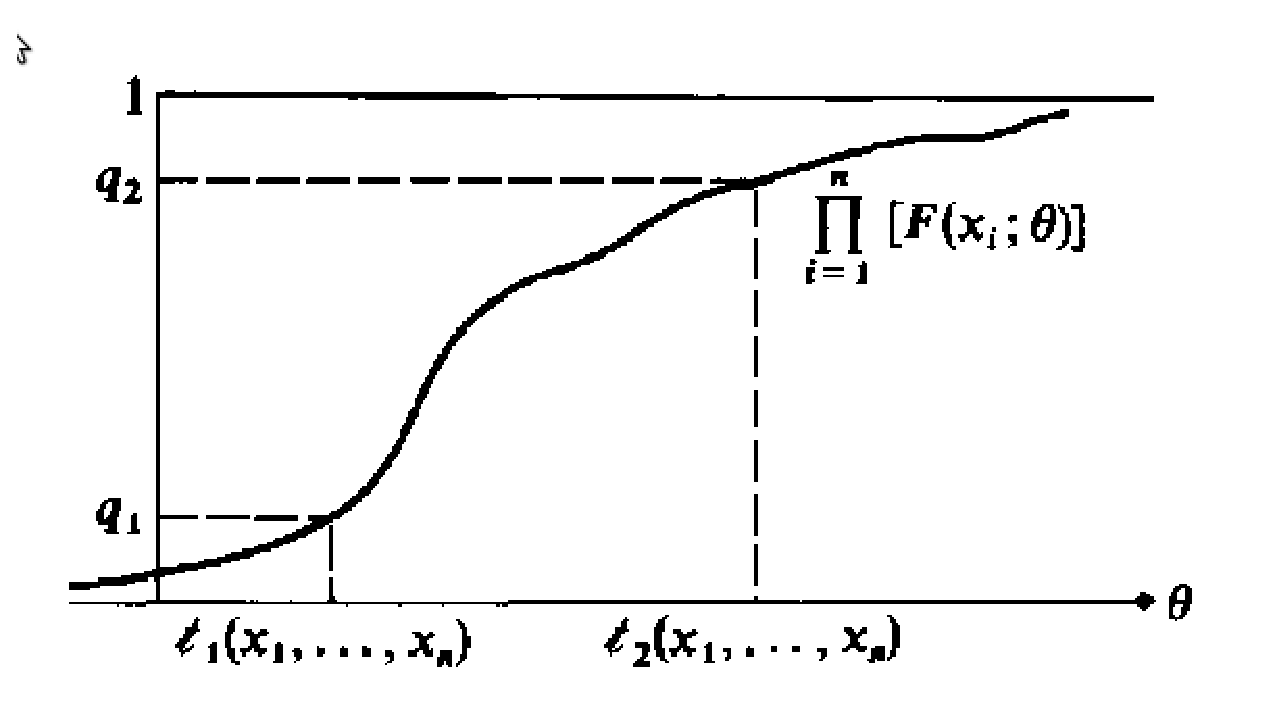
\includegraphics[scale = 0.5]{pictures/pivot_quantity_existence.eps}
\caption{Inverze pravděpodobnostní funkce}
\label{conf-interval-mu-sigma_a}
\end{figure}

\begin{example}
Uvažujme náhodný výběr $X_1, ..., X_n$ z populace $f(x, \theta) = \theta x^{\theta - 1}I_{(0, 1)}(x)$. Odpovídající kumulativní distribuční funkce má tedy tvar $F(x, \theta) = x^{\theta}I_{(0, 1)}(x) + I_{[1, \infty)}(x)$. Jestliže jsou $q_1$ a $q_2$ vybrány tak, že
\begin{gather*}
\gamma = P\left[q_1 < \prod_{i = 1}^n F(X_i, \theta) < q_2 \right] = P\left[q_1 < \prod_{i = 1}^n X_i^{\theta} < q_2 \right]\\
= P \left[\ln(q_1) < \theta \ln \left(\prod_{i = 1}^n X_i \right) < \ln(q_2)\right] = P \left[-\ln(q_2) < -\theta \ln \left(\prod_{i = 1}^n X_i \right) < -\ln(q_1) \right]\\
= P \left[\frac{\ln(q_2)}{\ln \left(\prod_{i = 1}^n X_i \right)} < \theta < \frac{\ln(q_1)}{\ln\left(\prod_{i = 1}^n X_i \right)}\right]
\end{gather*}
pak
\begin{equation*}
 \left(\frac{\ln(q_2)}{\ln \left(\prod_{i = 1}^n X_i\right)}, \frac{\ln(q_1)}{\ln\left(\prod_{i = 1}^n X_i \right)}\right)
\end{equation*}
představuje 100$\gamma$ procentní interval spolehlivosti pro $\theta$.
\end{example}

Závěrem uveďme poznámku ohledně existence centrální veličiny. Jestliže je $\theta$ lokační parametr, pak pravděpodobnostní funkce náhodné veličiny $X_i - \theta$ nezávisí na $\theta$, a proto je centrální veličinou stejně jako např. $\sum X_i - n \theta, Y_j - \theta$ a $Y_1 + Y_n - 2 \theta$. Jestliže je $\theta$ škálovací parametr, pak je pravděpodobnostní funkce náhodné veličiny $X_i / \theta$ nezávislá na $\theta$, a proto se jedná centrální veličinu. Centrálními veličinami jsou v tomto případě také $\sum X_i / \theta, Y_j / \theta$ apod.

\subsection{Statistiká metoda}

Opět uvažujme náhodný výběr $X_1, ..., X_n$ z populace $f(\cdot, \theta_0)$. Předpokládejme, že $\theta_0$, které v následujícím textu představuje skutečnou hodnotu parametru $\theta$, je reálné číslo a že $\overline{\underline{\Theta}}$ představuje interval na reálné ose. Pokusme se stanovit interval spolehlivosti pro $\theta_0$.

Nechť $T = \mathfrak{t}(X_1, ..., X_n)$ představuje statistiku, kterou vybereme jedním z následujících dvou způsobů. Jestliže existuje jednorozměrná dostatečná statistika, pak tuto statistiku použijeme namísto $T$. Jestliže dostatečná statistika neexistuje, pak pro $T$ použijeme bodovou funkci odhadu pro $\theta$. Konkrétní volba statistiky $T$ může také záviset na tom, jak složitá je její aplikace při konstrukci intervalu spolehlivosti - kritickým bodem je zejména odvození její pravděpodobnostní funkce.

Nechť $f_T(t, \theta)$ představuje pravděpodobnostní funkci statistiky $T$\footnote{V následujícím textu budeme předpokládat, že $T$ je spojitá náhodná veličina. Analogický postup však lze aplikovat také v případě nespojité náhodné veličiny.}. Definujme funkce $h_1(\theta)$ a $h_2(\theta)$, pro které platí
\begin{gather*}
\int_{-\infty}^{h_1(\theta)}f_T(t, \theta)dt = p_1\\
\int_{h_2(\theta)}^{\infty}f_T(t, \theta)dt = p_2\\
\end{gather*}
kde $p_1$ a $p_2$ jsou daná reálná čísla, která splňují podmínky $0 < p_1, 0 < p_2$ a $p_1 + p_2 < 1$. $h_1(\theta)$ a $h_2(\theta)$ lze znázornit jako funkce parametru $\theta$. Předpokládejme, že $h_1(\theta)$ a $h_2(\theta)$ jsou rostoucí funkce, pro které navíc platí $h_1(\theta) < h_2(\theta)$. Příklad dvou takovýchto funkcí ilustruje obrázek (\ref{h(1)-h(2)}).
\begin{figure}[htp]
\centering
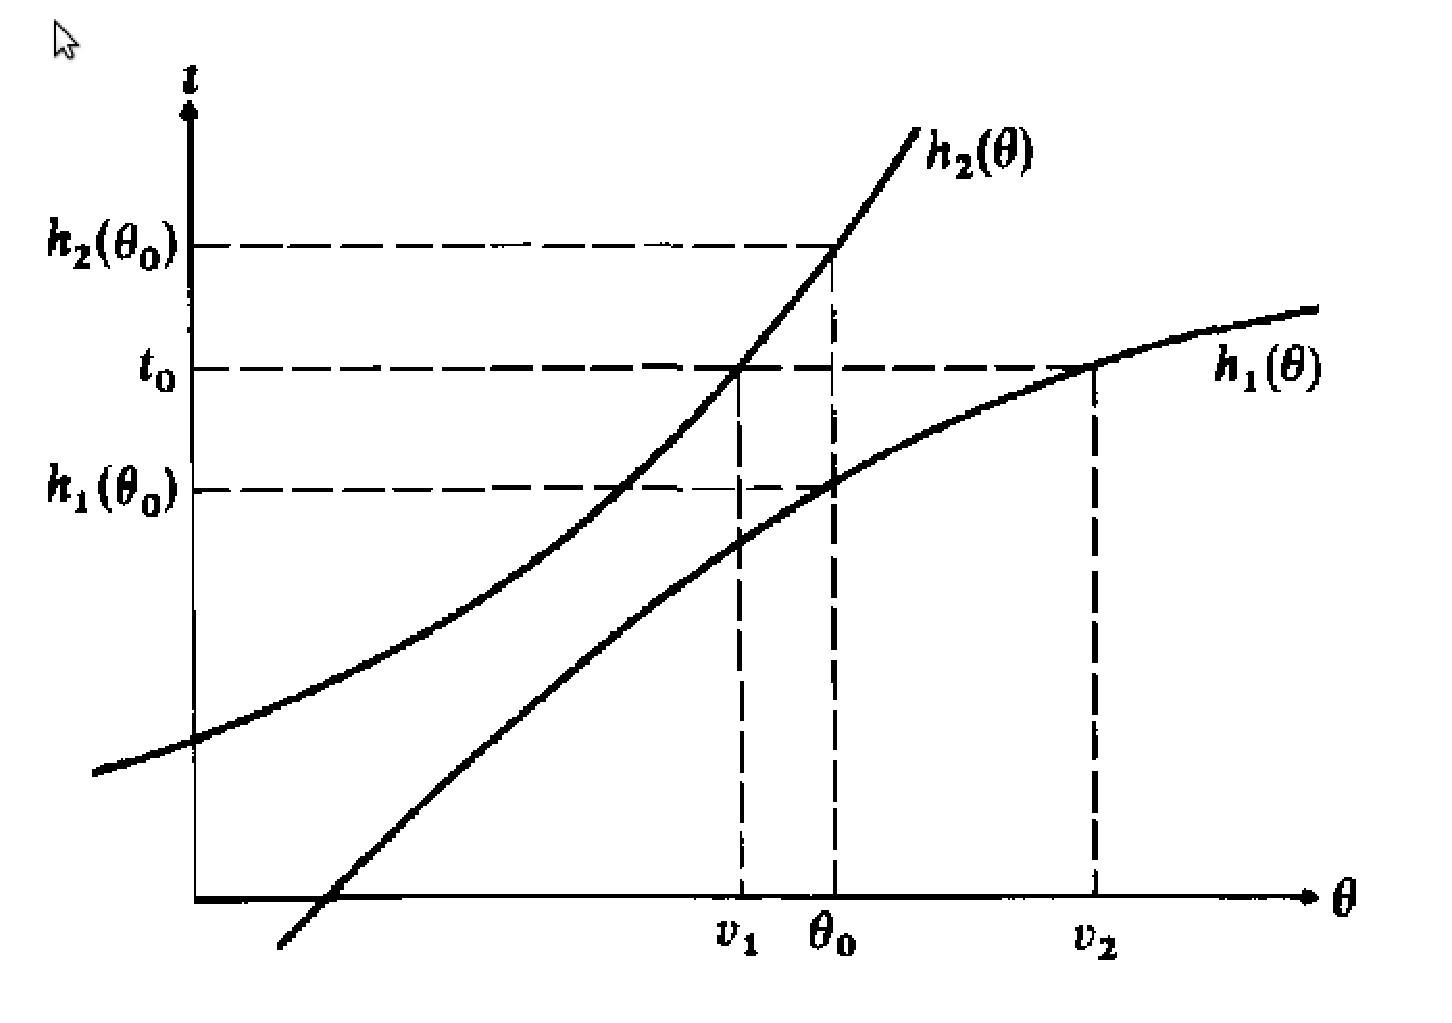
\includegraphics[scale = 0.5]{pictures/h(1)_h(2).eps}
\caption{Graf funkcí $h_1(\cdot)$ a $h_2(\cdot)$}
\label{h(1)-h(2)}
\end{figure}
Nechť $t_0$ označuje hodnotu statistiky $T$, tj. $t_0 = \mathfrak{t}(x_1, ..., x_n)$. Z této hodnoty lze, jak ilustruje obrázek (\ref{h(1)-h(2)}), získat hodnoty $v_1$ a $v_2$ takové, že $v_1 = \mathit{v_1(t_0)}$ a $v_1 = \mathit{v_2(t_0)}$. Z obrázku je dále zřejmé, že $h_1(\theta_0) < t_0 = \mathfrak{t}(x_1, ..., x_n) < h_2(\theta_0)$ platí pouze tehdy a jen tehdy, jestliže $v_1 = \mathit{v_1}(x_1, ..., x_n) < \theta_0 < v_2 = \mathit{v_2}(x_1, ..., x_n)$ pro libovolnou realizaci náhodného výběru $x_1, ..., x_n$. Z definice $h_1(\cdot)$ a $h_2(\cdot)$ však vyplývá
\begin{equation*}
P_{\theta_0}[h_1(\theta_0) < \mathfrak{t}(X_1, ..., X_n) < h_2(\theta_0)] = 1 - p_1 - p_2
\end{equation*}
a proto
\begin{equation*}
P_{\theta_0}[\mathit{v_1}(X_1, ..., X_n) < \theta_0 < \mathit{v_2}(X_1, ..., X_n)] = 1 - p_1 - p_2
\end{equation*}
Interval $(V_1, V_2)$ pak představuje 100$(1 - p_1 - p_2)$ procentní interval spolehlivosti pro $\theta_0$, kde $V_i = \mathit{v_i}(X_1, ..., X_n)$ pro $i = 1, 2$.

\begin{example}
Uvažujme náhodný výběr z populace $f(x, \theta_0) = \frac{1}{\theta_0}I_{(0, \theta_0)}(x)$. Pokusme se stanovit interval spolehlivosti pro $\theta_0$.

O $Y_n = \max(X_1, ..., X_n)$ víme, že se jedná o dostatečnou statistiku a že se jedná o funkci odhadu parametru $\theta_0$ založenou na metodě maximální věrohodnosti. Jestliže použijeme $Y_n$ jakožto statistiku $T$, pak
\begin{equation*}
f_T(t, \theta) = n \left(\frac{t}{\theta}\right)^{n - 1}\frac{1}{\theta}I_{(0, \theta)}(t)
\end{equation*}
$\int_0^{h_1(\theta)}n t^{n - 1}\theta^{-n}dt = p_1$ implikuje $\int_0^{h_1(\theta)}t^{n - 1}dt = \frac{\theta^n p_1}{n}$, což implikuje $\frac{\left(h_1(\theta) \right)^n}{n} = \frac{\theta^n p_1}{n}$ neboli $h_1(\theta) = \theta p_1^{1/n}$. Podobně $p_2 = \int_{h_2(\theta)}^{\theta}nt^{n - 1}\theta^{-n}dt$ implikuje $\theta^n - [h_2(\theta)]^n = \theta^n p_2$ neboli $h_2(\theta) = \theta(1 - p_2)^{1/n}$. Situaci ilustruje obrázek (\ref{h(1)-h(2)-example}), který je konkretizací obrázku (\ref{h(1)-h(2)}) v kontextu našeho příkladu.
\begin{figure}[htp]
\centering
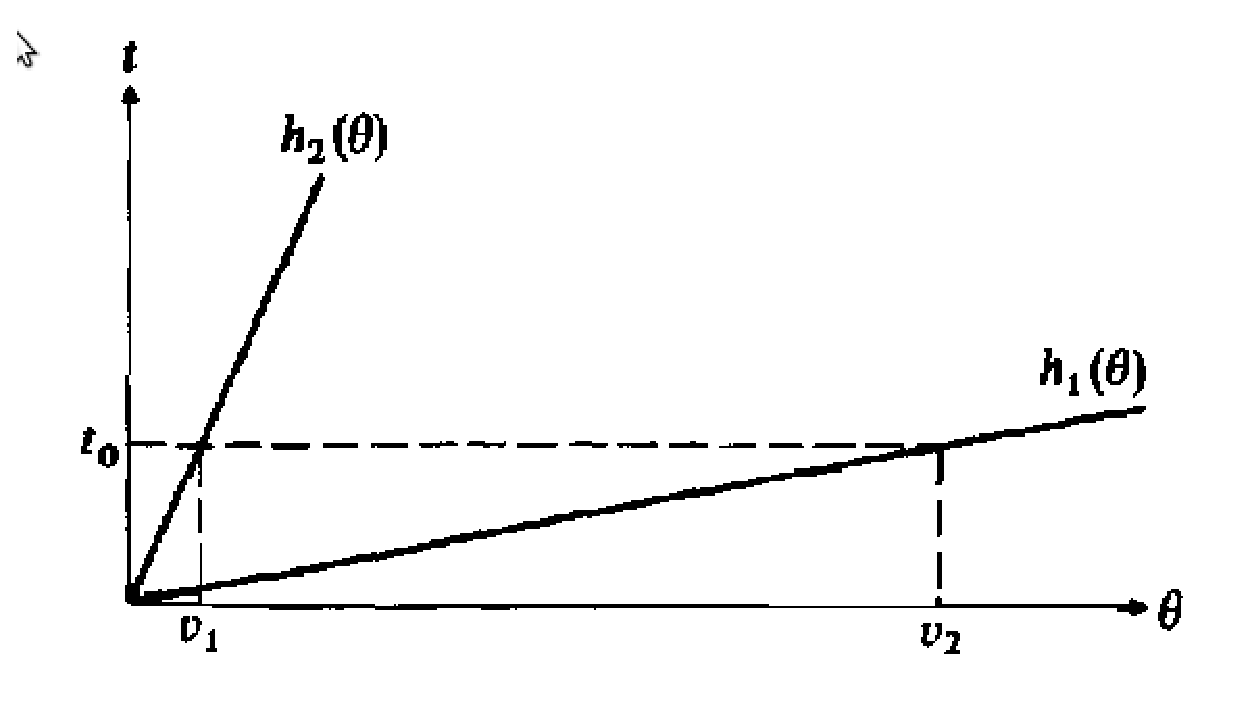
\includegraphics[scale = 0.5]{pictures/h(1)_h(2)_example.eps}
\caption{Graf funkcí $h_1(\cdot)$ a $h_2(\cdot)$}
\label{h(1)-h(2)-example}
\end{figure}
Pro $t_0 = \max(x_1, ..., x_n)$ je $v_1$ definováno jako $h_2(v_1) = t_0$, tj. $h_2(v_1) = v_1(1 - p_2)^{1/n} = t_0$ neboli $v_1 = t_0(1 - p_2)^{-1/n}$. Podobně lze odvodit $v_2 = t_0 p_1^{-1/n}$. To znamená, že 100$(1 - p_1 - p_2)$ procentní interval spolehlivosti pro $\theta_0$ je dán intervalem $(Y_n(1 - p_2)^{-1/n}, Y_n p_1^{-1/n})$.

Naším dalším cílem je stanovit $p_1$ a $p_2$ tak, aby interval spolehlivosti
\begin{equation*}
L = Y_n[p_1^{-1/n} - (1 - p_2)^{-1/n}]
\end{equation*}
byl pokud možno co nejkratší při splnění podmínek $1 - p_1 - p_2 = \gamma$ a $0 < p_1 + p_2 < 1$. To je splněno pro $p_2 = 0$ a $p_1 = 1 - \gamma$.
\end{example}

Z výše uvedeného příkladu je zřejmé, že funkce $h_1(\theta)$ a $h_2(\theta)$ nejsou vlastně potřeba. Pro danou hodnotu $t_0 = \mathfrak{t}(x_, ..., x_n)$ statistiky $T$ je zapotřebí nalézt $v_1 = \mathfrak{v}_1(x_1, ..., x_n)$ a  $v_2 = \mathfrak{v}_2(x_1, ..., x_n)$. $v_2$ lze získat řešením rovnice $p_1 = \int_{-\infty}^{h_1(\theta) = t_0} f_T(t, \theta) dt$ pro $\theta$. Podobně $v_2$ lze získat řešením rovnice $p_2 = \int_{h_(\theta) = t_0}^{\infty}f_T(t, \theta)dt$.

Výše uvedený postup lze aplikovat také pro nespojité náhodné veličiny. Jediným rozdílem bude nahrazení integrálů sumami.

\begin{example}
Uvažujme náhodný výběr $X_1, ..., X_n$ z Bernoulliho rozdělení $P[X = 1] = \theta_0 = 1 - P[X = 0]$. Víme, že $T = \sum X_i$ je dostatečná statistika s binomickým rozdělením, tj.
\begin{equation*}
P[T = t] = \binom{n}{t} \theta_0^t (1 - \theta_0)^{n - t}
\end{equation*}
pro $t = 0, 1, ..., n$. Pokusme se stanovit interval spolehlivosti pro $\theta_0$.

Předpokládejme, že $T = t_0$. Řešme rovnice
\begin{gather*}
p_1 = \sum_{t = 0}^{t_0} \binom{n}{t}\theta^t(1 - \theta)^{n - 1}\\
p_2 = \sum_{t = 0}^{t_0} \binom{n}{t}\theta^t(1 - \theta)^{n - 1}\\
\end{gather*}
pro $\theta$. Jestliže např. $p_1 = 0.0509, p_2 = 0.0159, n = 20$ a $T = 4$, pak je 93.33 procentní interval spolehlivosti parametru $\theta_0$ dán intervalem $(0.05, 0.40)$.
\end{example}

\section{Interval spolehlivosti pro výběry velkého rozsahu}

V případě bodového odhadu jsme ukázali, že v některých případech je možné nalézt posloupnost funkcí odhadu $T_n = \mathfrak{t}_n(X_1, ..., X_n)$ pro parametr $\theta$ pravděpodobnostního rozdělení $f(\cdot, \theta)$, které sledují asymptoticky normální rozdělení. To znamená, že $T_n$ asymptoticky sleduje normální rozdělení se střední hodnotou $\theta$ a rozptylem $\sigma_n^2(\theta)$. V kapitole (7.8) jsme ukázali, že v případě náhodného výběru velkého rozsahu sleduje funkce odhadu $\hat{\Theta}_n = \hat{\zeta}_n (X_1, ..., X_n)$ založená na metodě maximální věrohodnosti přibližně normální rozdělení se střední hodnotou $\theta$ a rozptylem
\begin{equation*}
\sigma_n^2(\theta) = \frac{1}{n E_{\theta}\left[\left(\frac{\partial}{\partial \theta}\ln\left(f(X, \theta)\right) \right)^2 \right]}
\end{equation*}
V tomto případě lze $\frac{T_n - \theta}{\sigma_n(\theta)}$ použít jako přibližnou centrální veličinu a příslušný 100$\gamma$ procentní interval spolehlivosti získat z nerovností
\begin{equation*}
-z < \frac{T_n - \theta}{\sigma_n(\theta)} < z
\end{equation*}
kde $z = z_{(1 + \gamma)/2}$ je definováno jako $\Phi(z_{(1 + z) / 2}) = (1 + \gamma) / 2$ neboli $\Phi(z) - \Phi(-z) = \gamma$. Tento postup lze aplikovat vždy, když lze z výše uvedených nerovností izolovat $\theta$.

\begin{example}
Uvažujme náhodný výběr $X_1, ..., X_n$ z populace $f(x, \theta) = \theta e^{-\theta x}I_{(0, \infty)}(x)$. Z příkladu (7.55) víme, že funkce odhadu dle metody maximální věrohodnosti pro $\theta$ má tvar $1 / \overline{X}_n$ a asymptoticky sleduje normální rozdělení se střední hodnotou $\theta$ a rozptylem
\begin{equation*}
\sigma_n^2(\theta) = \frac{1}{n E_{\theta}\left[\left(\frac{\partial}{\partial \theta} \ln \left(f(X, \theta)\right)\right)^2\right]} = \frac{\theta^2}{n}
\end{equation*}
Proto
\begin{gather*}
\gamma \approx P\left[-z < \frac{1 / \overline{X}_n - \theta}{\sqrt{\theta^2/n}} < z \right]\\
= P\left[-\frac{z \theta}{\sqrt{n}} < \frac{1}{\overline{X}_n} - \theta < \frac{z \theta}{\sqrt{n}} \right]\\
= P\left[\frac{1 / \overline{X}_n}{1 + z/\sqrt{n}} < \theta < \frac{1 / \overline{X}_n}{1 - z / \sqrt{n}} \right]
\end{gather*}
V případě náhodného výběru velkého rozsahu tak má 100$\gamma$ procentní interval spolehlivosti pro parametr $\theta$ tvar
\begin{equation*}
\left(\frac{1 / \overline{X}}{1 + z/\sqrt{n}}, \frac{1 / \overline{X}}{1 - z / \sqrt{n}}\right)
\end{equation*}
kde $z$ je definováno jako $\Phi(z) - \Phi(-z) = \gamma$.
\end{example}

\begin{example}
Uvažujme náhodný výběr velkého rozsahu z Bernoulliho rozdělení s parametry $\theta = P[X = 1] = 1 - P[X = 0]$. Funkce odhadu pro $\theta$ dle metody maximální věrohodnosti má tvar $\hat{\Theta} = \overline{X}_n$ a její rozptyl je $\sigma_n^2(\theta) = \theta(1 - \theta)/n$. 100$\gamma$ procentní interval spolehlivosti pro $\theta$ lze získat z nerovností
\begin{equation*}
P \left[\frac{2n \hat{\Theta} + z^2 - z \sqrt{4n \hat{\theta} + z^2 - 4n \hat{\Theta}^2}}{2(n + z^2)} < \theta < \frac{2n \hat{\Theta} + z^2 + z \sqrt{4n \hat{\theta} + z^2 - 4n \hat{\Theta}^2}}{2(n + z^2)} \right] \approx \gamma
\end{equation*}
Vzhledem k tomu, že předmětem našeho zájmu je náhodný výběr velkého rozsahu, lze všechny členy výše uvedených nerovností, které obsahují $1/\sqrt{n}$ resp. $1 / n$, zanedbat. Tím se dostáváme k
\begin{equation*}
P\left[\hat{\Theta} - z \sqrt{\frac{\hat{\Theta} - (1 - \hat{\Theta})}{n}} < \theta < \hat{\Theta} + z \sqrt{\frac{\hat{\Theta}(1 - \hat{\Theta})}{n}} \right] \approx \gamma
\end{equation*} 
\end{example}
Vztah odvozený ve výše uvedeném příkladě je vztahem, který bychom získali, pokud bychom v $\sigma_n^2(\theta)$ použily $\hat{\Theta}$ namísto $\theta$. Tato substituce by implikovala, že $\frac{\hat{\Theta} - \theta}{\sqrt{\hat{\Theta}(1 - \hat{\Theta})/n}}$ je přibližně normálně rozdělené s nulovou střední hodnotou a jednotkovým rozptylem. Tento závěr, který však nebudeme dokazovat, je obecně platný. To znamená, že funkce odhadu $\hat{\Theta}$ dle metody maximální věrohodnosti asymptoticky sleduje normální rozdělení se střední hodnotou $\theta$ a rozptylem $\sigma_n^2(\theta)$, který lze v případě náhodného výběru dostatečně velkého rozsahu aproximovat pomocí $\sigma_2^n(\Theta)$. Je zřejmé, že toto zjištění velmi zjednoduší konstrukci intervalu spolehlivosti, protože
\begin{equation*}
P\left[-z < \frac{\hat{\Theta} - \theta}{\sigma_n(\hat{\Theta})} < z \right] \approx \gamma
\end{equation*}
lze snadno převést do tvaru
\begin{equation*}
P[\hat{\Theta} - z \sigma_n(\hat{\Theta}) < \theta < \hat{\Theta} + z \sigma_n(\hat{\Theta})] \approx \gamma
\end{equation*}

Závěrem uveďme, že interval spolehlivosti pro náhodný výběr velkého rozsahu založený na funkci odhadu dle metody maximální věrohodnosti je optimální. To znamená, že je v průměru kratší než interval spolehlivosti založený na alternativních funkcích odhadu.

\section{Bayesovský interval}

Následující text navazuje na kapitolu (7.6). Uvažujme náhodný výběr z pravděpodobnostní funkce $f(\cdot|\theta)$, jejíž funkční předpis je znám. Připomeňme, že $\theta$ je hodnota náhodné veličiny $\Theta$, která je charakterizována apriorní pravděpodobnostní funkcí $g_{\Theta}(\cdot)$. Posteriorní pravděpodobnostní funkce náhodné veličiny $\Theta$ pro dané $(X_1, ..., X_n) = (x_1, ..., x_n)$ má tvar
\begin{equation*}
f_{\Theta|X_1 = x_1, ..., X_n = x_n}(\theta|x_1, ..., x_n) = \frac{\left[\prod_{i = 1}^n f(x_i|\theta) \right]}{\int \left[\prod_{i = 1}^n f(x_i|\theta) \right]g_{\Theta}(\theta)d\theta}
\end{equation*}
Pro fixní $\gamma$ je libovolný interval $(t_1, t_2)$ splňující podmínku
\begin{equation*}
\int_{t_1}^{t_2}f_{\Theta|X_1 = x_1, ..., X_n = x_n}(\theta|x_1, ..., x_n)d\theta = \gamma
\end{equation*}
100$\gamma$ procentním Bayesovským intervalem odhadu pro prameter $\theta$. V praxi bychom se snažili zvolit taková $t_1$ a $t_2$, aby délka intervalu byla co nejmenší. Dále platí, že $t_i = \mathit{t_i}(x_1, ..., x_n)$, tj. na $t_i$ lze pohlížet jako na funkci pozorování $x_1, ..., x_n$.

\begin{example}
Uvažujme náhodný výběr $X_1, ..., X_n$ z normálního rozdělení se střední hodnoto $\theta$ a jednotkovým rozptylem. Předpokládejme, že $\Theta$ má normální rozdělení se střední hodnotou $x_0$ a rozptylem 1. Pokusme se odhadnout $\theta$.

Z příkladu (7.48) víme, že posteriorní rozdělení náhodné veličiny $\Theta$ sleduje normální rozdělení se střední hodnotou $\frac{\sum_{i = 0}^n}{n + 1}$ a rozptylem $\frac{1}{n + 1}$. Hledáme $t_1$ a $t_2$, která splňují podmínku
\begin{gather*}
\gamma = \int_{t_1}^{t_2} f_{\Theta|X_1 = x_1, ..., X_n = x_n}(\theta|x_1, ..., x_n)d\theta\\
= \Phi\left(\frac{t_2 - \sum_{i = 0}^n \frac{x_i}{n + 1}}{\sqrt{1 / (n + 1)}}\right) - \Phi\left(\frac{t_1 - \sum_{i = 0}^n \frac{x_i}{n + 1}}{\sqrt{1 / (n + 1)}}\right)
\end{gather*}
Jestliže zvolíme $z$ takové, že $\Phi(z) - \Phi(-z) = \gamma$, pak
\begin{gather*}
t_2 = \frac{\sum_{i = 0}^n x_i}{n + 1} + z\sqrt{\frac{1}{n + 1}}\\
t_1 = \frac{\sum_{i = 0}^n x_i}{n + 1} - z\sqrt{\frac{1}{n + 1}}
\end{gather*}
definuje nejkratší Bayesovský interval odhadu pro $\theta$. Odpovídající interval spolehlivosti založený na metodě maximální věrohodnosti je dán intervalem $\left(\frac{\sum x_i}{n} - z\sqrt{\frac{1}{n}}, \frac{\sum x_i}{n} + z\sqrt{\frac{1}{n}} \right)$. Jediný rozdíl mezi těmito dvěma metodami spočívá v tom, že v případě Baysovského intervalu je velikost náhodného výběru zdánlivě navýšena o jedna, kde toto ``dodatečné'' pozorování je představováno střední hodnotou apriorního normálního rozdělení náhodné veličiny $\Theta$. 
\end{example}

\chapter{Testování hypotéz}

\section{Základní pojmy}

\begin{definition}[Statistiká hypotéza]
Statistickou větou se rozumí tvrzení a pravděpodobnostním rozdělení jedné nebo více náhodných veličin. Jestliže statistická hypotéza plně specifikuje toto pravděpodobnostní rozdělení, nazýváme ji jednoduchou statistickou hypotézou. V opačném případě mluvíme o tzv. složené statistické hypotéze.
\end{definition}

\begin{example}
Uvažujme náhodný výběr $X_1, ..., X_n$ z populace $f(x, \theta) = \phi_{\theta, 25}(x)$. Statistickou hypotézu, že střední hodnota tohoto normálního rozdělení je menší nebo rovna 17, zapisujeme jako $\mathscr{H}: \theta \le 17$. Takto definovaná hypotéza je složená, protože plně nespecifikuje normální rozdělení. Naproti tomu hypotéza, že střední hodnota normálního rozdělení je rovna 17, tj. $\mathscr{H}: \theta = 17$, je jednoduchou statistickou hypotézou.
\end{example}

\begin{definition}[Test statistiké hypotézy]
Testem statistické hypotézy $\mathscr{H}$ s rozumí pravidlo, na základě kterého se tato hypotéza přijme popř. zamítne. Test statistické hypotézy značíme jako $\mathscr{T}$.
\end{definition}

\begin{example}
Uvažujme náhodný výběr $X_1, ..., X_n$ z populace $f(x, \theta) = \phi_{\theta, 25}(x)$. Definujme statistickou hypotézu $\mathscr{H}: \theta \le 17$. Jedním z možných testů této hypotézy je zamítnutí $\mathscr{H}$, jestliže $\overline{X} > 17 + 5 / \sqrt{n}$.
\end{example}

Test hypotézy může být náhodný popř. nenáhodný. Test $\mathscr{T}$ z výše uvedeného příkladu je testem nenáhodným. Alternativní test $\mathscr{T}'$ hypotézy $\mathscr{H}$ z výše uvedeného příkladu by mohl spočívat v hodu mincí a následném zamítnutí $\mathscr{H}$, pokud by padla panna. Takovýto test by byl testem náhodným.

Stejně jako v předchozím textu budeme $\mathfrak{X}$ používat pro označení výběrového prostoru pozorování, tj. $\mathfrak{X} = \{(x_1, ..., x_n) : (x_1, ..., x_n) ~ \textit{představují všechny možné kombinace náhodných veličin}~(X_1, ..., X_n)\}$. 

\begin{definition}[Nenáhodný test a kritický region]
Uvažujme test $\mathscr{T}$ statistické hypotézy $H$, který tuto hypotézu zamítne, jestliže $(x_1, ..., x_n) \in C_{\mathscr{T}}$, kde $C_{\mathscr{T}}$ je podmnožinou $\mathfrak{X}$. Pak test $\mathscr{T}$ nazýváme nenáhodným testem a $C_{\mathscr{T}}$ jeho kritickým regionem.
\end{definition}

\begin{example}
Uvažujme náhodný výběr $X_1, ..., X_n$ z populace $f(x, \theta) = \phi_{\theta, 25}(x)$, tj. $\mathfrak{X}$ je $n$-rozměrný euklidovský prostor. Dále uvažujme hypotézu $\mathscr{H}: \theta \le 17$ a test $\mathscr{T}$, který zavrhuje tuto hypotézu pro $\overline{x} > 17 + 5 / \sqrt{n}$. Pak je $\mathscr{T}$ nenáhodným testem a $C_{\mathscr{T}} = \{(x_1, ..., x_n): \overline{x} > 17 + 5 / \sqrt{n} \}$.
\end{example}

V případě nenáhodného testu $\mathscr{T}$ hypotézy $\mathscr{H}$ je tak $\mathfrak{X}$ rozděleno na $C_{\mathscr{T}}$ a $\overline{C}_{\mathscr{T}}$ takové, že pro $(x_1, ..., x_n) \in C_{\mathscr{T}}$ je $\mathscr{H}$ zamítnuto. Nenáhodný test je tak specifikován svým kritickým regionem.

\begin{definition}[Náhodný test]
Test $\mathscr{T}$ hypotézy $\mathscr{H}$ je náhodný, jestliže je $\mathscr{T}$ definován funkcí\
\begin{equation*}
\psi_{\mathscr{T}}(x_1, ..., x_n) = P[\mathscr{H}~\textit{je zamítnuta pro realizaci náhodného výběru}~(x_1, ..., x_n)]
\end{equation*}
Tuto funkci nazýváme kritickou funkcí testu $\mathscr{T}$.
\end{definition}

Při aplikaci náhodného testu $\mathscr{T}$ hypotézy $\mathscr{H}$ je pro realizovaný náhodný výběr $(x_1, ..., x_n)$ ohodnocena funkce $\psi_{\mathscr{T}}(x_1, ..., x_n)$. Následně je proveden pomocný výběr z Bernoulliho rozdělení s pravděpodobností úspěchu $\psi_{\mathscr{T}}(x_1, ..., x_n)$. Jestliže tento výběr indikuje ``úspěch'', je $\mathscr{H}$ zamítnuta. Z tohoto popisu je zřejmé, že náhodné testy nejsou v praxi příliš používané. V některých případech je $\mathfrak{X}$ rozděleno na tři části, kde pro jednu je $\mathscr{H}$ přijato, pro druhou je $\mathscr{H}$ zamítnuto a pro třetí, která představuje ``šedou zónu'', je aplikován náhodný test. Situaci ilustruje následující příklad.

\begin{example}
Uvažujme náhodný výběr $X_1, ..., X_{10}$ z populace $f(x, \theta) = \theta^x(1 - \theta)^{1 - x}$ pro $x = 0, 1$. Předpokládejme, že chceme testovat hypotézu $\mathscr{H}: \theta < \frac{1}{2}$. Jedním z možných testů je $\mathscr{T}$ definovaný jako
\begin{enumerate}
\item zamítni $\mathscr{H}$, jestliže $\sum_{i = 1}^{10} x_i > 5$,
\item přijmi $\mathscr{H}$, jestliže $\sum_{i = 1}^{10} x_i < 5$ a
\item hoď mincí\footnote{Hod mincí zde zastupuje pomocný výběr z Bernoulliho rozdělení.} a rozhodni, jestliže $\sum_{i = 1}^{10} x_i = 5$
\end{enumerate}
Test $\mathscr{T}$ tedy rozděluje $\mathfrak{X}$ na tři části $A, B$ a $C$, kde
\begin{gather*}
A = \left\{(x_1, ..., x_{10}: \sum_{i = 1}^{10}x_i < 5)\right\}\\
B = \left\{(x_1, ..., x_{10}: \sum_{i = 1}^{10}x_i = 5)\right\}\\
C = \left\{(x_1, ..., x_{10}: \sum_{i = 1}^{10}x_i > 5)\right\}\\
\end{gather*}
Kritická funkce testu $\mathscr{T}$ je pak definována jako
\begin{equation*}
\psi_{\mathscr{T}(x_1, ..., x_n)} =
\begin{cases}
1 ~ \textit{pro} ~ (x_1, ..., x_{10}) \in C\\
\frac{1}{2} ~ \textit{pro} ~ (x_1, ..., x_{10}) \in B\\
0 ~ \textit{pro} ~ (x_1, ..., x_{10}) \in A
\end{cases}
\end{equation*}
\end{example}

V předchozím textu jsme uvedli, že nenáhodný test je specifikován svým kritickým regionem a že stejnou úlohu v případě náhodného testu pak plní kritická funkce. Platí, že libovolná funkce $\psi(\cdot, ..., \cdot)$ s definičním oborem $\mathfrak{X}$ a oborem hodnot $[0, 1]$ je možnou kritickou funkcí, která definuje náhodný test.

Jestliže je test $\mathscr{T}$ definován kritickou funkcí
\begin{equation*}
\psi_{\mathscr{T}}(x_1, ..., x_n) =
\begin{cases}
1 ~ \textit{pro} ~ (x_1, ..., x_n) \in C_{\mathscr{T}}\\
0 ~ \textit{v ostatních případech}
\end{cases}
\end{equation*}
pak je $\mathscr{T}$ nenáhodným testem s kritickým regionem $C_{\mathscr{T}}$.

Při testování hypotéz se rozhodujeme mezi tzv. nulovou hypotézou $\mathscr{H}_0$ a alternativní hypotézou $\mathscr{H}_1$. Logika rozhodování je taková, že je-li $\mathscr{H}_0$ zamítnuta, pak je přijata $\mathscr{H}_1$ a naopak. Při tomto postupu se můžeme dopustit dvou druhů chyb.

\begin{definition}[Typy chyb při testování hypotéz]
Chyba, které se dopustíme, jestliže zamítneme $\mathscr{H}_0$, která je ve skutečnosti pravdivá, je tzv. chybou typu I. Naopak přijetím $\mathscr{H}_0$, která je však ve skutečnosti nepravdivá, se dopouštíme chyby typu II. Velikosti chyb typu I a II jsou definovány pravděpodobnostmi, že se těchto chyb dopustíme.
\end{definition}

Jestliže je pravděpodobnostní rozdělení, ze kterého provádíme náhodný výběr, funkcí parametru $\theta$, kde $\theta \in \overline{\underline{\Theta}}$, pak lze každému testu přiřadit tzv. funkci charakteristické veličiny.

\begin{definition}[Funkce charakteristické veličiny]
Uvažujme test $\mathscr{T}$ nulové hypotézy $\mathscr{H}_0$. Funkce charakteristické veličiny testu $\mathscr{T}$ je označována $\pi_{\mathscr{T}}(\theta)$ a je definována jako pravděpodobnost zamítnutí $\mathscr{H}_0$, jestliže pravděpodobností rozdělení, ze kterého byl prováděn náhodný výběr, je funkcí parametru $\theta$.
\end{definition}

Funkce charakteristické veličiny plní stejnou roli jako MSE v případě bodového odhadu - v následujícím textu bude představovat standardní nástroj pro porovnání daného testu s alternativními testy. Z definice je zřejmé, že ideální funkce charakteristické veličiny nabývá nulové hodnoty pro $\theta$, která odpovídají nulové hypotéze, a jednotkové hodnoty pro $\theta$, která odpovídají alternativní hypotéze.

Platí, že $\pi_{\mathscr{T}}(\theta) = P_{\mathscr{T}}[\textit{zamítnutí}~\mathscr{H}_0]$, kde $\theta$ představuje skutečnou hodnotu parametru. Jestliže je $\mathscr{T}$ nenáhodným testem, pak $\pi_{\mathscr{T}}(\theta) = P_{\theta}[(X_1, ..., X_n) \in C_{\mathscr{T}}]$, kde $C_{\mathscr{T}}$ je kritickým regionem testu $\mathscr{T}$. Jestliže je $\mathscr{T}$ náhodným testem s kritickou funkcí $\psi_{\mathscr{T}}(\cdot, ..., \cdot)$, pak
\begin{multline*}
\pi_{\mathscr{T}} = P_{\mathscr{T}}[\textit{zamítnutí}~\mathscr{H}_0]\\
= \int \cdots \int P[\textit{zamítnutí}~\mathscr{H}_0 | x_1, ..., x_n]f_{X_1, ..., X_n}(x_1, ..., x_n; \theta) \prod_{i = 1}^n d x_i\\
= \int \cdots \int \psi_{\mathscr{T}}(x_1, ..., x_n)f_{X_1, ..., X_n}(x_1, ..., x_n; \theta)\prod_{i = 1}^n d x_i = E_{\theta}[\psi_{\mathscr{T}}(X_1, ..., X_n)]
\end{multline*}
Analogické odvození lze provést také v případě nespojité náhodné veličiny.

\begin{example}
Uvažujme náhodný výběr $X_1, ..., X_n$ z populace $f(x, \theta) = \phi_{\theta, 25}(x)$. Uvažujme nulovou hypotézu $\mathscr{H}_0: \theta \le 17$ a test $\mathscr{T}$, který zavrhuje $\mathscr{H}_0$, jestliže $\overline{X} > 17 + 5 / \sqrt{n}$. Funkce charakterické veličiny je dána rovnicí
\begin{equation*}
\pi_{\mathscr{T}}(\theta) = P_{\theta}\left[\overline{X} > 17 + \frac{5}{\sqrt{n}} \right] = 1 - \Phi\left(\frac{17 + 5 / \sqrt{n} - \theta}{5 / \sqrt{n}}\right)
\end{equation*}
Pro $n = 25$ je $\pi_{\mathscr{T}}(\theta)$ ilustrována obrázkem (\ref{power-function}). Funkce charakteristiké veličiny indikuje, nakolik je daný test spolehlivý. Jestliže je v našem konkrétním případě $\theta$ větší než 20, pak test $\mathscr{T}$ správně zamítne $\mathscr{H}_0$. Naopak, jestliže je $\theta$ menší než 16, pak test $\mathscr{T}$, opět správně, s vysokou pravděpodobností $\mathscr{H}_0$ nezamítne. Jestliže je však $17 < \theta < 18$, je pravděpodobnost zamítnutí $\mathscr{H}_0$ na základě testu $\mathscr{T}$ méně než poloviční, ačkoliv je hypotéza $\mathscr{H}_0$ nepravdivá.
\end{example}

\begin{figure}[htp]
\centering
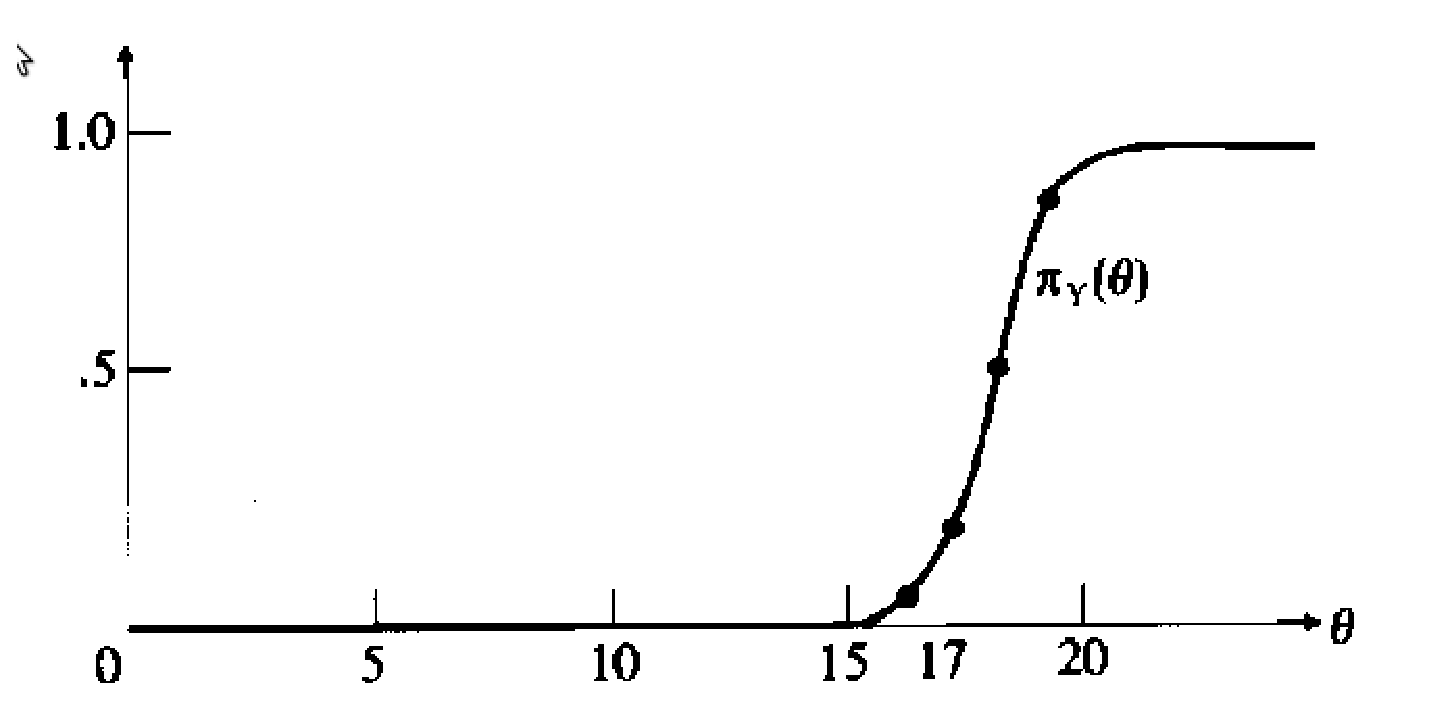
\includegraphics[scale = 0.5]{pictures/power_function.eps}
\caption{Funkce charakteristické veličiny}
\label{power-function}
\end{figure}

\begin{definition}[Velikost testu]
Uvažujme test $\mathscr{T}$ hypotézy $\mathscr{H}_0: \theta \in \overline{\underline{\Theta}}_0$, kde $\overline{\underline{\Theta}}_0 \subset \overline{\underline{\Theta}}$. Velikost testu $\mathscr{T}$ je definována jako $\sup_{\theta \in \overline{\underline{\Theta}}_0}[\pi_{\mathscr{T}}(\theta)]$. Velikost nenáhodného testu je někdy také nazývána velikostí kritického regionu.
\end{definition}

\begin{example}
Uvažujme náhodný výběr $X_1, ..., X_n$ z populace $f(x, \theta) = \phi_{\theta, 25}(x)$. Dále uvažujme hypotézu $\mathscr{H}_0: \theta \le 17$ a test $\mathscr{T}$, který zavrhuje $\mathscr{H}_0$ jestliže $\overline{X} > 17 + 5 / \sqrt{n}$. Platí $\overline{\underline{\Theta}}_0 = \{\theta: \theta \le 17\}$ a velikost testu $\mathscr{T}$ je
\begin{equation*}
\sup_{\theta \in \overline{\underline{\Theta}}_0}[\pi_{\mathscr{T}}(\theta)] = \sup_{\theta \le 17}\left[1 - \Phi\left(\frac{17 + 5 / \sqrt{n} - \theta}{5 / \sqrt{n}}\right)\right] = 1 - \Phi(1) \approx 0.159
\end{equation*}
\end{example}

\begin{theorem}
Uvažujme náhodný výběr $X_1, ..., X_n$ z populace $f(x, \theta)$, kde $\theta \in \overline{\underline{\Theta}}$ a soubor dostatečných statistik $S_1 = \mathfrak{s}_1(X_1, ..., X_n), ..., S_r = \mathfrak{s}_r(X_1, ..., X_n)$. Pak pro libovolný test $\mathscr{T}$ s kritickou funkcí $\psi_{\mathscr{T}}(X_1, ..., X_n)$ existuje test $\mathscr{T}'$ s kritickou funkcí $\psi_{\mathscr{T}'}(S_1, ..., S_r)$, která splňuje $\pi_{\mathscr{T}}(\theta) = \pi_{\mathscr{T}'}(\theta)$ pro všechna $\theta \in \overline{\underline{\Theta}}$.
\end{theorem}

\begin{proof}
Definujme $\psi_{\mathscr{T}'}(s_1, ..., s_r) = E[\psi_{\mathscr{T}}(X_1, ..., X_n)|S_1 = s_1, ..., S_r = s_r]$, pak $\psi_{\mathscr{T}'}$ je kritickou funkcí. Dále platí $\pi_{\mathscr{T}'}(\theta) = E_{\theta}[\psi_{\mathscr{T}'}(S_1, ..., S_r)] = E_{\theta}[E[\psi_{\mathscr{T}}(X_1, ..., X_n)|S_1, ..., S_r]] = E_{\theta}[\psi_{\mathscr{T}}(X_1, ..., X_n)] = \pi_{\mathscr{T}}(\theta)$.
\end{proof}

Z výše uvedené věty vyplývá, že pro libovolný test existuje alternativní test založený pouze na souboru dostatečných statistik a že tento test má stejnou funkci charakteristické veličiny jako test původní. Při našem pátrání po vhodném testu se tak můžeme omezit pouze na testy založených právě na souboru dostatečných statistik.

\section{Testování jednoduchých hypotéz}

\begin{definition}[Jednoduchý věrohodnostní poměrový test]
Uvažujme náhodný výběr $X_1, ..., X_n$, o kterém víme, že pochází buď z populace $f_0(\cdot)$ nebo $f_1(\cdot)$. Test $\mathscr{T}$, který testuje $\mathscr{H}_0: X_i \sim f_0(\cdot)$ proti $\mathscr{H}_1: X_i \sim f_1(\cdot)$, je nazýván jednoduchým věrohodnostním poměrovým testem, jestliže je definován jako
\begin{enumerate}
\item zamítni $\mathscr{H}_0$, jestliže $\lambda < k$,
\item přijmi $\mathscr{H}_0$, jestliže $\lambda > k$,
\item přijmi / zamítni $\mathscr{H}_0$ popř. rozhodni na základě náhodného testu, jestliže $\lambda = k$
\end{enumerate}
kde
\begin{equation*}
\lambda = \lambda(x_1, ..., x_n) = \frac{\prod_{i = 1}^n f_0(x_i)}{\prod_{i = 1}^n f_1(x_i)} = \frac{L_0(x_1, ..., x_n)}{L_1(x_1, ..., x_n)} = \frac{L_0}{L_1}
\end{equation*}
a $k$ je nezáporná konstanta. Připomeňme, že $L_j = L_j(x_1, ..., x_n)$ je funkce maximální věrohodnosti pro náhodný výběr z populace $f_j(\cdot)$.
\end{definition}

Pro fixní $k$ tedy test zavrhuje $\mathscr{H}_0$ pro nízké hodnoty $\lambda$ a naopak. Výsledek testu tedy zavisí na zvolené hodnotě $k$.

Jednoduchý věrohodnostní poměrový test je v souladu s intuicí. Navíc lze očekávat, že ``optimální'' test bude mít podobu právě jednoduchého věrohodnostního poměrového testu. K hledání ``optimálního'' testu pro jednoduché hypotézy lze přistoupit dvěma způsoby - prvním z nich je koncept tzv. nejsilnějšího testu a druhý spočívá ve využití ztrátové funkce.

\subsection{Nejsilnější test}

Uvažujme náhodný výběr $X_1, ..., X_n$, o kterém víme, že pochází buď z populace $f_0(\cdot)$ nebo $f_1(\cdot)$, kde $f_0(x) = f(x, \theta_0)$ a $f_1(x) = f(x, \theta_1)$ a $\theta_0$ a $\theta_1$ jsou známé konstanty. To znamená, že $\overline{\underline{\Theta}} = \{\theta_0, \theta_1\}$ je prostor, který se skládá z pouchých dvou bodů. Testujme hypotézu $\mathscr{H}_0: \theta = \theta_1$ proti hypotéze $\mathscr{H}_1: \theta = \theta_1$. Tomuto testu lze přiřadit funkci charakteristické veličiny $\pi_{\mathscr{T}}(\theta)$. Dobrý test je takový, pro který je $\pi_{\mathscr{T}}(\theta_0) = P[\textit{zamítnutí} ~ \mathscr{H}_0|\mathscr{H}_0 ~ \textit{je pradivá}]$ malé (ideálně rovno nule) a $\pi_{\mathscr{T}}(\theta_0) = P[\textit{zamítnutí} ~ \mathscr{H}_0|\mathscr{H}_0 ~ \textit{je nepradivá}]$ vysoké (ideálně rovno jedné).  $\pi_{\mathscr{T}}(\theta_0)$ odpovídá chybě typu I a $1 - \pi_{\mathscr{T}}(\theta_1) = P[\textit{přijetí} ~ \mathscr{H}_0 | \mathscr{H}_0 ~ \textit{je nepravdivá}]$ odpovídá chybě typu II. Naším cílem je minimalizovat obě chyby. Možných postupů je několik.

\begin{definition}[Nejsilnější test]
Test $\mathscr{T}^*$, který testuje $\mathscr{H}_0: \theta = \theta_0$ proti $\mathscr{H}_1: \theta = \theta_1$ je nejsilnějším testem velikosti $\alpha$, kde $0 < \alpha < 1$, jestliže
\begin{enumerate}
\item $\pi_{\mathscr{T}^*}(\theta_0) = \alpha$
\item $\pi_{\mathscr{T}^*}(\theta_1) \ge \pi_{\mathscr{T}}(\theta_1)$ pro libovolný alternativní test $\mathscr{T}$, pro který platí $\pi_{\mathscr{T}}(\theta_0) \le \alpha$.
\end{enumerate}
\end{definition}

Důvod, proč fixujeme velikost chyby typu I na úroveň $\alpha$\footnote{$\alpha$ je nastaveno zpravidla na nízkou úroveň - obvyklé hodnoty jsou 0.01 a 0.05.} zatímco velikost chyby typu II nikoliv, je skutečnost, že nulová a alternativní hypotéza jsou zpravidla formulovány tak, že realizace chyby typu I má závažnější následky než realizace chyby typu II.

\begin{theorem}[Neyman-Pearsonova]
Uvažujme náhodný výběr $X_1, ..., X_n$ z populace $f(x, \theta)$, kde $\theta$ nabývá hodnoty $\theta_0$ nebo $\theta_1$. Předpokládejme, že $\alpha$, kde $0 < \alpha < 1$, je fixní a známé. Nechť $k^*$ je pozitivní konstanta a $C^*$ je podmnožina $\mathfrak{X}$, která splňuje
\begin{enumerate}
\item $P_{\theta_0}[(X_1, ..., X_n) \in C^*] = \alpha$
\item $\lambda = \frac{L(\theta_0; x_1, ..., x_n)}{\theta_1; x_1, ..., x_n} = \frac{L_0}{L_1} \le k^*$ pro $(x_1, ..., x_n) \in C^*$
\item  $\lambda \ge k^*$ pro $(x_1, ..., x_n) \in \overline{C}^*$
\end{enumerate}
Pak je test $\mathscr{T}^*$, který je charakterizován kritickým regionem $C^*$, nejsilnějším testem velikosti $\alpha$ pro testování $\mathscr{H}_0: \theta = \theta_0$ proti $\mathscr{H}_1: \theta = \theta_1$. Připomeňme, že $L_j = L(\theta_j; x_1, ..., x_n) = \prod_{i = 1}^n f(x_i, \theta_j)$ pro $j = 0, 1$. $\overline{C}^*$ je doplněk k $C^*$, tj. $\overline{C}^* = \mathfrak{X} - C^*$
\end{theorem}

\begin{proof}
Předpokládejme, že existují taková $k^*$ a $C^*$, která splňují podmínky (1) až (3) výše uvedené věty. Uvažujme alternativní test $\mathscr{T}$ se silou alespoň $\alpha$ a kritickým regionem $C$, tj. $P_{\theta_0}[(X_1, ..., X_n) \in C] \le \alpha$.

V následujícím textu budeme pro libovolné $R \subset \mathfrak{X}$ namísto $\int \cdots \int_{R}\left[\prod_{i = 1}^n f(x_i, \theta_j)dx_i\right]$ používat zkrácený zápis $\int_R L_j$, kde $j = 0, 1$. Ze zápisu vyplývá, že $f_0(\cdot)$ a $f_1(\cdot)$ jsou pravděpodobnostní funkce spojité náhodné veličiny. Stejný důkaz nicméně platí také pro nespojité náhodné veličiny.

Musíme dokázat $\pi_{\mathscr{T}^*}(\theta_1) \ge \pi_{\mathscr{T}}(\theta_1)$, což je ekvivalentní důkazu $\int_{C^*} L_1 \ge \int_C L_1$. Následující postup ilustruje obrázek (\ref{most-power-test}). Platí
\begin{equation*}
\int_{C^*}L_1 - \int_C L_1 = \int_{C^* \overline{C}}L_1 - \int_{C \overline{C}^*}L_1 \le \frac{1}{k^*}\int_{C^* \overline{C}}L_0 - \frac{1}{k^*}\int_{C \overline{C}^*}L_0
\end{equation*}
protože $L_1 \ge \frac{L_0}{k^*}$ na množině $C^*$ (a tím pádem také na množině $C^* \overline{C}$) a $L_1 \le \frac{L_0}{k^*}$ neboli $-L_1 \ge -\frac{L_0}{k^*}$ na množině $\overline{C}^*$ (a tím pádem také na množině $C \overline{C}^*$). Nicméně
\begin{multline*}
\frac{1}{k^*}\left(\int_{C^* \overline{C}}L_0 - \int_{C\overline{C}^*}L_0\right) = \frac{1}{k^*}\left(\int_{C^*\overline{C}}L_0 - \int_{C^* C}L_0 + \int_{C^* C}L_0 - \int_{C \overline{C}^*}L_0\right)\\
= \frac{1}{k^*}\left(\int_{C^*} L_0 - \int_C L_0 \right) = \frac{1}{k^*}(\alpha - \textit{velikost testu} ~ \mathscr{T})
\end{multline*}
což implikuje $\int_{C^*}L_1 - \int_C L_1 \ge 0$.
\end{proof}

\begin{figure}[htp]
\centering
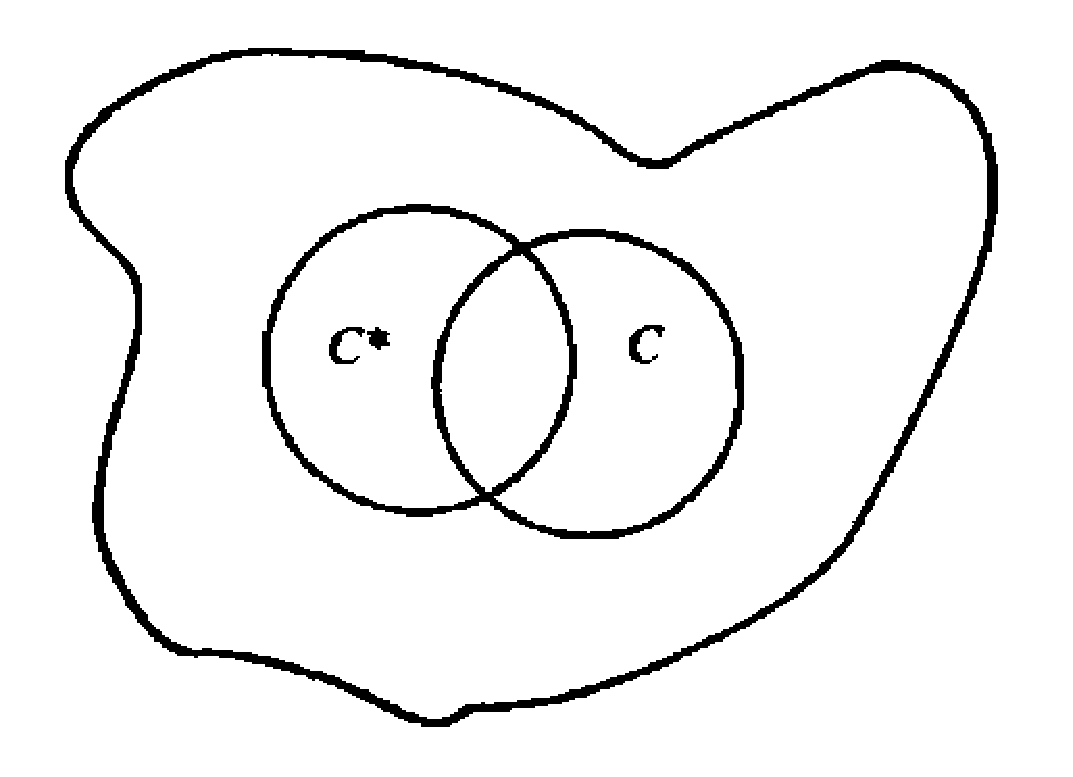
\includegraphics[scale = 0.5]{pictures/most_powerful_test.eps}
\caption{Ilustrační obrázek}
\label{power-function}
\end{figure}

Obecně platí, že ne vždy musí existovat $k^*$ a $C^*$, která splňují podmínky Neyman-Pearsovy věty. V takovém případě  Neyman-Pearsovy věta není schopná dát nejsilnější test síly $\alpha$. Nicméně jestliže jsou $f_0(\cdot)$ a $f_1(\cdot)$ pravděpodobnostními funkcemi spojité náhodné veličiny, pak odpovídající $k^*$ a $C^*$ vždy existují.
Ačkoliv Neyman-Pearsovy věty explicitně neříká, jak nalézt $k^*$ a $C^*$, jsou $k^*$ a $C^*$ dány implicitně její druhou podmínkou.

\begin{example}
Uvažujme náhodný výběr $X_1, ..., X_n$ z populace $f(x, \theta) = \theta e^{-\theta x}I_{0, \infty}(x)$, kde $\theta = \theta_0$ popř. $\theta = \theta_1$. $\theta_0$ a $\theta_1$ jsou fixní a známé. Předpokládejme $\theta_0 < \theta_1$. Definujme test $\mathscr{T}$, který testuje hypotézu $\mathscr{H}_0: \theta = \theta_0$ proti hypotéze $\mathscr{H}_1: \theta = \theta_1$.

Potřebné funkce maximální věrohodnosti mají tvar $L_0 = \theta_0^n e^{-\theta_0 \sum x_i}$ a $L_1 = \theta_1^n e^{-\theta_1 \sum x_i}$. Dle Neyman-Pearsonovy věty zamítne nejsilnější test $\mathscr{H}$, jestliže $\lambda \le k^*$, což lze v kontextu našeho příkladu vyjádřit jako
\begin{gather*}
\left(\frac{\theta_0}{\theta_1}\right)^n e^{-(\theta_0 - \theta_1)\sum_{i = 1}^n x_i} \le k^*\\
\sum_{i = 1}^n x_i \frac{1}{\theta_1 - \theta_0}\ln \left[\left(\frac{\theta_1}{\theta_0}\right)^n k^* \right] = k'
\end{gather*}
kde $k'$ je opět konstanta. Nerovnost $\lambda \le k^*$ tak byla zjednodušena a vyjádřena ve tvaru $\sum x_i \le k'$. První podmínka má tvar
\begin{equation*}
\alpha = P_{\theta_0}[\textit{zamítnutí} ~ \mathscr{H}_0] = P_{\theta_0}\left[\sum_{i = 1}^n X_i \le k' \right]
\end{equation*}
Víme, že $\sum x_i$ sleduje gamma rozdělení s parametry $n$ a $\theta$, a proto lze $k'$ vypočíst z rovnice
\begin{equation*}
P_{\theta_0}\left[\sum_{i = 1} X_i \le k' \right] = \int_0^{k'} \frac{1}{\Gamma(n)} \theta_0^n x^{n - 1}e^{-x \theta_0}dx = \alpha
\end{equation*}
Nejsilnější test $\mathscr{T}$ velikosti $\alpha$ pro $\mathscr{H}_0: \theta = \theta_0$ vs. $\mathscr{H}_1: \theta = \theta_1$, kde $\theta_0 < \theta_1$ zamítne $\mathscr{H}_0$ jestliže $\sum x_i \le k'$, kde $k'$ je $\alpha$-tý kvantil gamma rozdělení s parametry $n$ a $\theta_0$.
\end{example}

\begin{example}
Uvažujme náhodný výběr $X_1, ..., X_n$ z populace $f(x, \theta) = \theta^x(1 - \theta)^{1 - x}I_{\{0, 1\}}(x)$, kde $\theta = \theta_0$ popř. $\theta = \theta_1$ a $\theta_0 < \theta_1$. Potřebné funkce maximální věrohodnosti mají tvar $L_0 = \theta_0^{\sum_{i = 1}^n x_i}(1 - \theta_0)^{n - \sum_{i = 1}^n x_i}$ a $L_1 = \theta_1^{\sum_{i = 1}^n x_i}(1 - \theta_1)^{n - \sum_{i = 1}^n x_i}$. Nerovnost $\lambda < k^*$ je tedy splněna, jestliže
\begin{gather*}
\frac{\theta_0^{\sum_{i = 0}^n x_i}(1 - \theta_0)^{n - \sum_{i = 1}^n x_i}}{\theta_1^{\sum_{i = 0}^n x_i}(1 - \theta_1)^{n - \sum_{i = 1}^n x_i}} \le k^*\\
\left[\frac{\theta_0(1 - \theta_1)}{(1 - \theta_1)\theta_1}\right]^{\sum_{i = 1}^n x_i} \left(\frac{1 - \theta_0}{1 - \theta_1}\right)^n \le k^*
\end{gather*}
neboli, jestliže $\sum x_i \ge k'$, kde $k'$ je konstanta\footnote{Připomeňme, že $\ln \left(\frac{\theta_0 (1 - \theta_1)}{(1 - \theta_0)\theta_1}\right) < 0$.}.

Předpokládejme, že $\theta_0 = 1/4$, $\theta_1 = 3/4$ a $n = 10$. Musíme nalézt $k'$ takové, že
\begin{equation*}
\alpha = P_{\theta_0 = 1/4}[\textit{zamítnutí} ~ \mathscr{H}_0] = P_{\theta_0 = 1/4}\left[\sum_{i = 1}^n X_i \ge k' \right] = \sum_{i = k'}^{10}\binom{10}{i}\left(\frac{1}{4}\right)^i\left(\frac{3}{4}\right)^{10 - i}
\end{equation*}
Jestliže $\alpha = 0.0197$, pak $k' = 6$. Jestliže $\alpha = 0.0781$, pak $k' = 5$. Pro $\alpha = 0.05$ však neexistuje kritický region $C^*$ a konstanta $k^*$ dle Neyman-Pearsonovy věty. V tomto příkladě je totiž námi uvažovaná náhodná veličina diskrétní a pro diskrétní náhodné veličiny není vždy možné nalézt $C^*$ a $k^*$ pro libovolné $\alpha$. Tento problém je možné obejít např. změnou velikosti náhodného výběru. Nicméně nejsilnější test velikosti $\alpha$ existuje vždy, pouze se může jednat o náhodný test. V našem konkrétním případě lze pro $\alpha = 0.05$ definovat tento test jako
\begin{equation*}
\psi(x_1, ..., x_{10}) =
\begin{cases}
1 ~ \textit{pro} ~ \sum_{i = 1}^n x_i \ge 6\\
\frac{0.05 - 0.0197}{0.0584} ~ \textit{pro} ~ \sum_{i = 1}^n = 5\\
0 ~ \textit{pro} ~ \sum_{i = 1}^n x_i \le 4
\end{cases}
\end{equation*}
\end{example}

\subsection{Ztrátová funkce}

Stejně jako v předchozím textu uvažujme náhodný výběr $X_1, ..., X_n$ z populace $f(x, \theta)$, kde $\theta = \theta_0$ nebo $\theta = \theta_o$ a testujme $\mathscr{H}_0: \theta = \theta_0$ vs. $\mathscr{H}_1: \theta = \theta_1$. Můžeme tedy učinit dvě rozhodnutí - rozhodnutí $d_0$, že náhodný výběr pochází z populace $f(x, \theta_0)$ a rozhodnutí $_1$, že náhodný výběr pochází z populace $f(x, \theta_1)$. Předpokládejme, že máme k dispozici ztrátovou funkci.

\begin{definition}[Ztrátová funkce]
Pro účely testování $\mathscr{H}_0: \theta = \theta_0$ vs. $\mathscr{H}_1: \theta = \theta_1$ definujme $\mathfrak{l}(d_i, \theta_j) = \textit{ztráta z rozhodnutí} ~ d_i ~ \textit{jestliže správná hodnota parametru je} ~ \theta_j$. Přijmněme konvenci $\mathfrak{l}(d_i, \theta_i) = 0$ a $\mathfrak{l}(d_i, \theta_j) > 0$ pro $i \neq j$.
\end{definition}

V kontextu nenáhodného testu $\mathscr{T}$ s kritickým regionem $C_{\mathscr{T}}$ je učiněno rozhodnutí $d_1$, jestliže $(x_1, ..., x_n)$ náleží do $C_{\mathscr{T}}$ a rozhodnutí $d_0$, jestliže $(x_1, ..., x_n)$ náleží do $\overline{C}_{\mathscr{T}}$. Jestliže je přijato rozhodnutí $d_1$, avšak správná hodnota parametru je $\theta_0$, dopouštíme se chyby typu I. Podobně, jestliže je přijato rozhodnutí $d_0$, avšak správná hodnota parametru je $\theta_1$, dopouštíme se chyby typu II.

Při výběru testu pochopitelně preferujeme ten s nejmenší ``ztrátou''. Bohužel v praxi jen zřídka existuje jen jeden test, který má nejmenší ``ztrátu'' pro obě možná rozhodnutí a všechna možná $\theta_0$ a $\theta_1$. Tímto se dostáváme k tzv. rizikové funkci.

\begin{definition}[Riziková funkce]
Uvažujme náhodný výběr $X_1, ... ,X_n$, o kterém víme, že pochází s populace $f(\cdot, \theta_0)$ nebo $f(\cdot, \theta_1)$. Nechť test $\mathfrak{T}$ s kritickým regionem $C_{\mathscr{T}}$ testuje  $\mathscr{H}_0: \theta = \theta_0$ vs. $\mathscr{H}_1: \theta = \theta_1$. Uvažujme danou ztrátovou funkci $\mathfrak{l}(\cdot, \cdot)$. Riziková funkce $\mathscr{r}_{\mathscr{T}}(0)$ testu $\mathscr{T}$ je definována jako očekávaná ztráta, tj.
\begin{equation*}
\mathfrak{r}_{\mathscr{T}}(\theta) = \int \cdots \int_{C_{\mathscr{T}}} \mathfrak{l}(d_1, \theta)\left[\prod_{i = 1}^n f(x_i, \theta) d x_i\right] + \int \cdots \int_{\overline{C}_{\mathscr{T}}}\mathfrak{l}(d_0, \theta)\left[\prod_{i = 1}^n f(x_i, \theta) d x_i \right]
\end{equation*} 
\end{definition}

Všimněme si, že riziková funkce je lineární funkcí funkce charakteristické veličiny, kde koeficienty v této lineární funkci jsou dány hodnotou ztrátové funkce.
\begin{multline*}
\mathfrak{r}_{\mathscr{T}}(\theta) = \mathfrak{l}(d_1, \theta)P_{\theta}[(X_1, ..., X_n) \in C_{\mathscr{T}}] + \mathfrak{l}(d_0, \theta)P_{\theta}[(X_1, ..., X_n) \in \overline{C}_{\mathscr{T}}]\\
= \mathfrak{l}(d_1, \theta) \pi_{\mathfrak{T}}(\theta) + \mathfrak(d_0, \theta)[1 - \pi_{\mathfrak{T}}(\theta)]
\end{multline*}
Vzhledem k tomu, že parametr $\theta$ může nabývat pouze dvou hodnot, může pouze dvou hodnot nabývat také riziková funkce. Konkrétně se jedná o hodnoty
\begin{gather*}
\mathfrak{r}_{\mathscr{T}}(\theta_0) = \mathfrak{l}(d_1, \theta_0)\pi_{\mathscr{T}}(\theta_0)\\
\mathfrak{r}_{\mathscr{T}}(\theta_1) = \mathfrak{l}(d_0, \theta_1)[1 - \pi_{\mathscr{T}}(\theta_1)]
\end{gather*}

Ideální test je charakterizován nejmenším ``rizikem'' v porovnání se všemi možnými alternativními testy. Problém však spočívá v tom, že ``riziko'' nabývá dvou hodnot a test, který by v porovnání se všemi možnými alternativními testy dosahoval minima pro obě tyto hodnoty, existuje pouze ve vyjímečných případech. Tímto se dostáváme ke konceptu minimax testu.

\begin{definition}[Minimax test]
Test $\mathscr{T}_m$ pro $\mathscr{H}_0: \theta = \theta_0$ vs. $\mathscr{H}_1: \theta = \theta_1$ je minimaxem, jestliže
\begin{equation*}
\max[\mathfrak{r}_{\mathscr{T}_m}(\theta_0), \mathfrak{r}_{\mathscr{T}_m}(\theta_1)] \le \max[\mathfrak{r}_{\mathscr{T}}(\theta_0), \mathfrak{r}_{\mathscr{T}}(\theta_1)] 
\end{equation*}
pro libovolný alternativní test.
\end{definition}

Následující větu je někdy možné použít při hledání minimax testu.

\begin{theorem}
Uvažujme náhodný výběr $X_1, ... ,X_n$, o kterém víme, že pochází s populace $f(\cdot, \theta_0)$ nebo $f(\cdot, \theta_1)$. Dále uvažujme test $\mathfrak{T}_m$, který testuje $\mathscr{H}_0: \theta = \theta_0$ vs. $\mathscr{H}_1: \theta = \theta_1$. Jestliže kritický region testu $\mathfrak{T}_m$ je definován jako $C_m = \{(x_1, ..., x_n): \lambda \le k_m \}$, kde $k_m$ je kladná konstanta taková, že $\mathfrak{r}_{\mathfrak{T}_m}(\theta_0) = \mathfrak{r}_{\mathfrak{T}_m}(\theta_1)$, pak je $\mathscr{T}_m$ minimaxem. Připomeňme, že
\begin{equation*}
\lambda = \frac{L_0}{L_1} = \frac{\prod_{i = 1}^n f(x_i, \theta_0)}{\prod_{i = 1}^n f(x_i, \theta_1)}
\end{equation*} 
\end{theorem}

\begin{proof}
Předpokládejme, že $f(\cdot, \theta_0)$ a $f(\cdot, \theta_1)$ jsou pravděpodobnostní funkce spojitých náhodných veličin. Důkaz pro nespojité náhodné veličiny by byl analogický.

Uvažujme alternativní test $\mathscr{T}$ s kritickým regionem $C_{\mathscr{T}}$, který splňuje podmínku $\mathfrak{r}_{\mathscr{T}}(\theta_0) \le \mathfrak{r}_{\mathscr{T}_m}(\theta_0)$\footnote{Pokud by platilo $\mathfrak{r}_{\mathscr{T}}(\theta_0) > \mathfrak{r}_{\mathscr{T}_m}(\theta_0)$, pak by test $\mathscr{T}$ nemohl být ani kandidátem na minimax.}, což implikuje
\begin{gather*}
\mathfrak{l}(d_1, \theta_0)\pi_{\mathscr{T}}(\theta_0) \le \mathfrak{l}(d_1, \theta_0)\pi_{\mathscr{T}_m}(\theta_0)\\
\pi_{\mathscr{T}}(\theta_0) \le \pi_{\mathscr{T}_m}(\theta_0)
\end{gather*}
tj. $\mathscr{T}$ má velikost menší nebo rovnu velikosti testu $\mathscr{T}_m$. Nicméně na základě Neyman-Pearsonovy věty je $\mathscr{T}_m$ nejsilnějším testem velikosti $\pi_{\mathscr{T}_m}(\theta_0)$. Proto platí
\begin{gather*}
\pi_{\mathscr{T}}(\theta_1) \le \pi_{\mathscr{Y}_m}(\theta_1)\\
1 - \pi_{\mathscr{T}}(\theta_1) \ge 1 - \pi_{\mathscr{T}_m}(\theta_1)\\
\mathfrak{l}(d_0, \theta_1)[1 - \pi_{\mathscr{T}}(\theta_0)] \ge \mathfrak{l}(d_0, \theta_1)[1 - \pi_{\mathscr{T}_m}(\theta_0)]\\
\mathfrak{r}_{\mathscr{T}}(\theta_1) \ge \mathfrak{r}_{\mathscr{T}_m}(\theta_1)
\end{gather*}
a proto
\begin{equation*}
\max[\mathfrak{r}_{\mathscr{T}_m}(\theta_0), \mathfrak{r}_{\mathscr{T}_m}(\theta_1)] = \mathfrak{r}_{\mathscr{T}_m}(\theta_1) \le \mathfrak{r}_{\mathscr{T}}(\theta_1) \le \max[\mathfrak{r}_{\mathscr{T}}(\theta_0), \mathfrak{r}_{\mathscr{T}}(\theta_1)]
\end{equation*}
tj. $\mathscr{T}_m$ je minimaxem.
\end{proof}

\begin{example}
Uvažujme náhodný výběr $X_1, ..., X_n$ z populace $f(x, \theta) = \theta e^{-\theta x}I_{(0, \infty)}(x)$. Pro $\theta_1 > \theta_0$ testujme $\mathscr{H}_0: \theta = \theta_0$ vs. $\mathscr{H}_1: \theta = \theta_0$. V příkladu (9.7) jsme nalezli nejsilnější test velikosti $\alpha$. Pokusme se nyní nalézt minimax test pro ztrátovou funkci definovanou jako $\mathfrak{d_1, \theta_0} = a$ a $\mathfrak{d_0, \theta_1} = b$.

Dle výše uvedené věty je minimax test $\mathfrak{T}_m$ dán $C_m = \{(x_1, ..., x_n): \lambda \le k_m\}$, kde $k_m$ definováno rovností $\mathfrak{r}_{\mathscr{T}_m}(\theta_0) = \mathfrak{r}_{\mathscr{T}_m}(\theta_1)$. Nerovnost $\lambda \le k_m$ lze vyjádřit jako $\sum x_i \le k$, kde $k$ je konstanta. Rovnost $\mathfrak{r}_{\mathscr{T}_m}(\theta_0) = \mathfrak{r}_{\mathscr{T}_m}(\theta_1)$ je splněna, jestliže $a \pi_{\mathscr{T}_m}(\theta_0) = b[1 - \pi_{\mathscr{T}_m}(\theta_1)]$, tj. hledáme takové $k$, které splňuje
\begin{gather*}
a P_{\theta_0}[\sum_{i = 1}^n X_i \le k] = b P_{\theta_1}[\sum_{i = 1}^n X_i > k]\\
a \int_0^k \frac{1}{\Gamma(n)}\theta_0^n x^{n - 1}e^{-\theta_0 x}dx = b \int_k^{\infty}\frac{1}{\Gamma(n)}\theta_1^n x^{n - 1}e^{-\theta_1 x}dx
\end{gather*}
\end{example}

Jestliže jsou $f_0(\cdot)$ a $f_1(\cdot)$ pravděpodobnostní funkce diskrétní náhodné veličiny, pak se může stát, že neexistuje takové $k_m$, pro které $\mathfrak{r}_{\mathscr{T}_m}(\theta_0) = \mathfrak{r}_{\mathscr{T}_m}(\theta_1)$, pokud nepřistoupíme na náhodné testy. Z věty (9.3) je zřejmé, že minimax je jednoduchým věrohodnostním poměrovým testem.

V předchozím textu jsme předpokládali, že funkční předpis $f(\cdot, \theta)$ je znám a že parametr $\theta$ může nabývat pouze dvou hodnot a to $\theta_0$ a $\theta_1$. Dále jsme předpokládali, že známe příslušnou ztrátovou funkci. Nyní však předpokládejme, že $\theta_0$ a $\theta_1$ jsou hodnoty náhodné veličiny $\Theta$, jejíž apriorní pravděpodobnostní funkci známe. Jedná se tedy o stejný koncept jako v případě Bayesovského odhadu. Náhodná veličina $\Theta$ je tedy nespojitá a nabývá pouze dvou hodnot a to $\theta_0$ a $\theta_1$. Apriorní pravděpodobnostní funkce $\Theta$ má tedy tvar $g = P[\Theta = \theta_1] = P[\Theta = \theta_0]$.

\begin{definition}[Bayesovský test]
Test $\mathscr{T}_g$, který testuje $\mathscr{H}: \theta = \theta_0$ proti $\mathscr{H}: \theta = \theta_1$ je Bayesovským testem s apriorní pravěpodobnostní funkcí
\begin{equation*}
g = P[\Theta = \theta_1]
\end{equation*}
právě tehdy a jen tehdy je-li splněna nerovnost
\begin{equation*}
(1 - g)\mathfrak{r}_{\mathscr{T}_g}(\theta_0) + g \mathfrak{r}_{\mathscr{T}_g}(\theta_1) \le (1 - g)\mathfrak{r}_{\mathscr{T}}(\theta_0) + g \mathfrak{r}_{\mathscr{T}}(\theta_1)
\end{equation*}
pro libovolný alternativní test $\mathscr{T}$. Abychom nalezli Bayesovský test, hledáme kritický region $C_g$, který minimalizuje
\begin{multline*}
(1 - g)\mathfrak{r}_{\mathscr{T}}(\theta_0) + g \mathfrak{r}_{\mathscr{T}}(\theta_1) = (1 - g)\mathfrak{l}(d_1, \theta_0)\pi_{\mathscr{T}}(\theta_0) + g \mathfrak{l}(d_0, \theta_1)[1 - \pi_{\mathscr{T}}(\theta_1)]\\
= (1 - g)\mathfrak{l}(d_1, \theta_0) \int_C L_0 + g \mathfrak{l}(d_0, \theta_1) \int_{\overline{C}}L_1
\end{multline*}
jakožto funkci regionu $C$. Zároveň však platí, že
\begin{multline*}
(1 - g)\mathfrak{l}(d_1, \theta_0)\int_C L_0 + g \mathfrak{l}(d_0, \theta_1) \int_{\overline{C}}L_1\\
= g \mathfrak{l}(d_0, \theta_1) + \int_C[(1 - g)\mathfrak{l}(d_1, \theta_0)L_0 - g \mathfrak{l}(d_0, \theta_1)L_1]
\end{multline*}
je minimální pro region $C$, který obsahuje všechna $(x_1, ..., x_n)$, pro která je poslední integrant záporný, tj.
\begin{equation*}
C_g = \{(x_1, ..., x_n): (1 - g)\mathfrak{l}(d_1, \theta_0)L_0 - g \mathfrak{l}(d_0, \theta_1)L_1 < 0\}
\end{equation*}
Tímto jsme zároveň dokázali následující větu.
\end{definition}

\begin{theorem}
Bayesovský test $\mathscr{T}_g$, který testuje $\mathscr{H}_0: \theta = \theta_0$ vs. $\mathscr{H}_1: \theta = \theta_1$ s ohledem na apriorní rozdělení $g = P[\Theta = \theta_1]$ má kritický region definovaný jako
\begin{equation*}
C_g = \left\{(x_1, ..., x_n): \lambda < \frac{g \mathfrak{l}(d_0, \theta_1)}{(1 - g)\mathfrak(d_1, \theta_0)}\right\}
\end{equation*}
To znamená, že Bayesovský test má opět charakter jednoduchého věrohodnostního poměrového testu.
\end{theorem}

\begin{example}
Uvažujme náhodný výběr $X_1, ..., X_n$ z populace $f(x, \theta) = \theta e^{-\theta x}I_{(0, \infty)}(x)$. Testujme $\mathscr{H}_0: \theta = \theta_0$ proti $\mathscr{H}_1: \theta = \theta_1$. Kritický region Bayesovského testu je dán
\begin{multline*}
C_g = \left\{(x_1, ..., x_n): \frac{\theta_0^n e^{-\theta_0 \sum_{i = 0}^n x_i}}{\theta_1^n e^{-\theta_1 \sum_{i = 0}^n x_i}} < \frac{g \mathfrak{l}(d_0, \theta_1)}{(1 - g)\mathfrak{l}(d_1, \theta_0)}\right\}\\
= \left\{(x_1, ..., x_n): \sum_{i = 1}^n x_i < \frac{1}{\theta_1 - \theta_0}\ln \left(\frac{g\theta_1^n\mathfrak{l}(d_0, \theta_1)}{(1 - g)\theta_0^n\mathfrak{l}(d_1, \theta_0)}\right)\right\}
\end{multline*}
pro $\theta_1 > \theta_0$.
\end{example}

\section{Testování složených hypotéz}

Předpokládejme náhodný výběr z populace $f(x, \theta)$, kde $\theta \in \overline{\underline{\Theta}}$. Dále předpokládejme, že chceme testovat $\mathscr{H}_0: \theta \in \overline{\underline{\Theta}}_0$ vs. $\mathscr{H}_1: \theta \in \overline{\underline{\Theta}}_1$, kde $\overline{\underline{\Theta}}_0 \subset \overline{\underline{\Theta}}$, $\overline{\underline{\Theta}}_1 \subset \overline{\underline{\Theta}}$ a $\overline{\underline{\Theta}}_0$ a $\overline{\underline{\Theta}}_1$ jsou disjunktní množiny. Obvykle platí $\overline{\underline{\Theta}}_1 = \overline{\underline{\Theta}} - \overline{\underline{\Theta}}_0$.

\subsection{Obecný věrohodnostní poměrový test}

Pro náhodný výběr $X_1, ..., X_n$ z populace $f(x, \theta)$, kde $\theta \in \overline{\underline{\Theta}}$ hledáme test $\mathscr{H}_0: \theta \in \overline{\underline{\Theta}}_0$ vs. $\mathscr{H}_1: \theta \in \overline{\underline{\Theta}}_1 = \overline{\underline{\Theta}} - \overline{\underline{\Theta}}_0$.

\begin{definition}[Obecný věrohodnostní poměr]
Uvažujme funkci maximální věrohodnosti $L(\theta; x_1, ..., x_n)$ náhodného výběru $X_1, ..., X_n$ se sdruženou pravděpodobnostní funkcí $f_{X_1, ..., X_n}(x_1, ..., x_n; \theta)$, kde $\theta \in \overline{\underline{\Theta}}$. Obecný věrohodnostní poměr $\lambda_n$ je definován jako
\begin{equation*}
\lambda_n = \lambda(x_1, ..., x_n) = \frac{\sup_{\theta \in \overline{\underline{\Theta}}_0} L(\theta; x_1, ..., x_n)}{\sup_{\theta \in \overline{\underline{\Theta}}_n}L(\theta; x_1, ..., x_n)}
\end{equation*}
\end{definition}

Všimněme si, že $\lambda_n$ je funkcí pozorování $x_1, ..., x_n$, tj. $\lambda_n = \lambda(x_1, ..., x_n)$. Jestliže tato pozorování nahradíme náhodnými veličinami $X_1, ..., X_n$, pak se dle zvyklostí změní zápis na $\Lambda = \lambda(X_1, ..., X_n)$. $\Lambda$ je tak funkcí náhodných veličin $X_1, ..., X_n$, a proto se jedná o náhodnou veličinu resp. o statistiku, protože nezávisí na neznámých parametrech.

V souvislosti s obecným věrohodnostním poměrem uveďme následujících pět poznámek.
\begin{enumerate}
\item Pro obecný věrohodnostní poměr používáme symbol $\lambda$, který jsme v předchozím textu používali pro jednoduchý věrohodnostní poměr. Avšak pro $\overline{\underline{\Theta}} = \{\theta_0, \theta_1\}$ se obecný věrohodnostní poměr nezredukuje na jednoduchý věrohodnostní poměr, jak by bylo možné se domnívat.
\item Obecný věrohodnostní poměr $\lambda$ splňuje podmínku $0 \le \lambda \le 1$. Nerovnost $\lambda \ge 0$ vyplývá ze skutečnosti, že $\lambda$ je poměrem dvou nezáporných čísel. Nerovnost $\lambda \le 1$ pak vyplývá ze skutečnosti, že suprémum v čitateli je přes $\overline{\underline{\Theta}}_0$ a suprémum ve jmenovateli přes $\overline{\underline{\Theta}}$, přičemž $\overline{\underline{\Theta}}_0 \subset \overline{\underline{\Theta}}$.
\item Parametr $\Theta$ může mít podobu vektoru.
\item Jmenovatel $\Lambda$ je představován hodnotou funkce maximální věrohodnosti pro funkci odhadu založené na metodě maximální věrohodnosti. 
\item V našich úvahách bude mít náhodný výběr $X_1, ..., X_n$ často podobu náhodného výběru z populace $f(x, \theta)$, kde $\theta \in \overline{\underline{\Theta}}$.
\end{enumerate}

Hodnoty $\lambda$ statistiky $\Lambda$ slouží k formulaci testu $\mathscr{H}_0: \theta \in \overline{\underline{\Theta}}_0$ vs. $\mathscr{H}_1: \theta \in \overline{\underline{\Theta}}_1 = \overline{\underline{\Theta}} - \overline{\underline{\Theta}}_0$, kde $\mathscr{H}_0$ je zamítnuta, jestliže $\lambda \le \lambda_0$, kde $\lambda_0$ představuje konstantu, která splňuje podmínku $0 \le \lambda_0 \le 1$ a která je často odvozena od síly testu.

V některých případech výše popsaná metoda naráží na skutečnost, že může být poměrně komplikované nalézt $\sup L(\theta; x_1, ..., x_n)$ nebo pravděpodobnostní rozdělení $\Lambda$, které je nezbytné pro stanovení síly testu.

\begin{example}
Uvažujme náhodný výběr $X_1, ..., X_n$ z populace $f(x, \theta) = \theta e^{-\theta x}I_{(0, \infty)}(x)$, kde $\overline{\underline{\Theta}} = \{\theta; \theta > 0\}$. Testujme  $\mathscr{H}_0: \theta \le \theta_0$ vs. $\mathscr{H}_1: \theta > \theta_0$.
\begin{equation*}
\sup_{\theta \in \overline{\underline{\Theta}}} L(\theta; x_1, ..., x_n) = \sup_{\theta > 0}\left(\theta^n e^{-\sum_{i = 1}^n x_i}\right) = \left(\frac{n}{\sum_{i = 1}^n x_i}\right)^n e^{-n}
\end{equation*}
a
\begin{multline*}
\sup_{\theta \in \overline{\underline{\Theta}}_0} L(\theta; x_1, ..., x_n) = \sup_{0 < \theta \le \theta_0}(\theta^n e^{-\theta \sum_{i = 1}^n x_i})\\
=
\begin{cases}
\left(\frac{n}{\sum_{i = 1}^n x_i}\right)^n e^{-n} ~ \textit{pro} ~ \frac{n}{\sum_{i = 1}^n} \le \theta_0\\
\theta_0^n e^{-\theta_0 \sum_{i = 1}^n x_i} ~ \textit{pro} ~ \frac{n}{\sum_{i = 1}^n} > \theta_0
\end{cases}
\end{multline*}
Proto
\begin{equation*}
\lambda =
\begin{cases}
1 ~ \textit{pro} ~ \frac{n}{\sum_{i = 1}^n} \le \theta_0\\
\frac{\theta_0^n e^{-\theta_0 \sum_{i = 1}^n x_i}}{\left(\frac{n}{\sum_{i = 1}^n x_i}\right)^n e^{-n}} ~ \textit{pro} ~ \frac{n}{\sum_{i = 1}^n > \theta_0}
\end{cases}
\end{equation*}
Pro $0 < \lambda_0 < 1$ tak obecný věrohodnostní poměrový test zamítne $\mathscr{H}_0$, jestliže
\begin{equation*}
\frac{n}{\sum_{i = 1}^n x_i} > \theta_0 ~ \textit{a} ~ \left(\frac{\theta_0 \sum_{i = 1}^n x_i}{n}\right)^n e^{-\theta_0 \sum_{i = 1}^n x_i + n} \le \lambda_0
\end{equation*}
což je ekvivaletní podmínkám
\begin{equation*}
\theta_0 \overline{x} < 1 ~ \textit{a} ~ (\theta_0 \overline{x})^n e^{-n(\theta_0 \overline{x} - 1)} \le \lambda_0
\end{equation*}
Jestliže použijeme substituci $y = \theta_0 \overline{x}$, pak má $y^ne^{-n(y - 1)}$ maximum v bodě $y = 1$. Proto $y < 1$ a $y^n e^{-n(y - 1)}$ je menší nebo rovno $\lambda_0$ pouze je-li $y \le k$, kde $k$ je konstanta splňující podmínku $0 < k < 1$. Situaci ilustruje obrázek (\ref{example_9_11}).

Obecný věrohodnostní poměrový test se tak zjednoduší do podoby, kdy $\mathscr{H}_0$ je zamítnuto, jestliže $\theta_0 \overline{x} < k$, kde $0 < k < 1$. Jestliže má tento test mít sílu $\alpha$, pak je $k$ řešením následující rovnice\footnote{Připomeňme, že $P_{\theta}[\theta_0 \overline{X} < k] \le P_{\theta_0}[\theta_0 \overline{X} < k]$ pro $\theta \le \theta_0$.}
\begin{equation*}
\alpha = P_{\theta_0}[\theta_0 \overline{X} < k] = P_{\theta_0}[\theta_0 \sum_{i = 1}^n X_i < nk] = \int_0^{nk} \frac{1}{\Gamma(n)}u^{n - 1}u^{n - 1}e^{-u}du
\end{equation*}
\end{example}

\begin{figure}[htp]
\centering
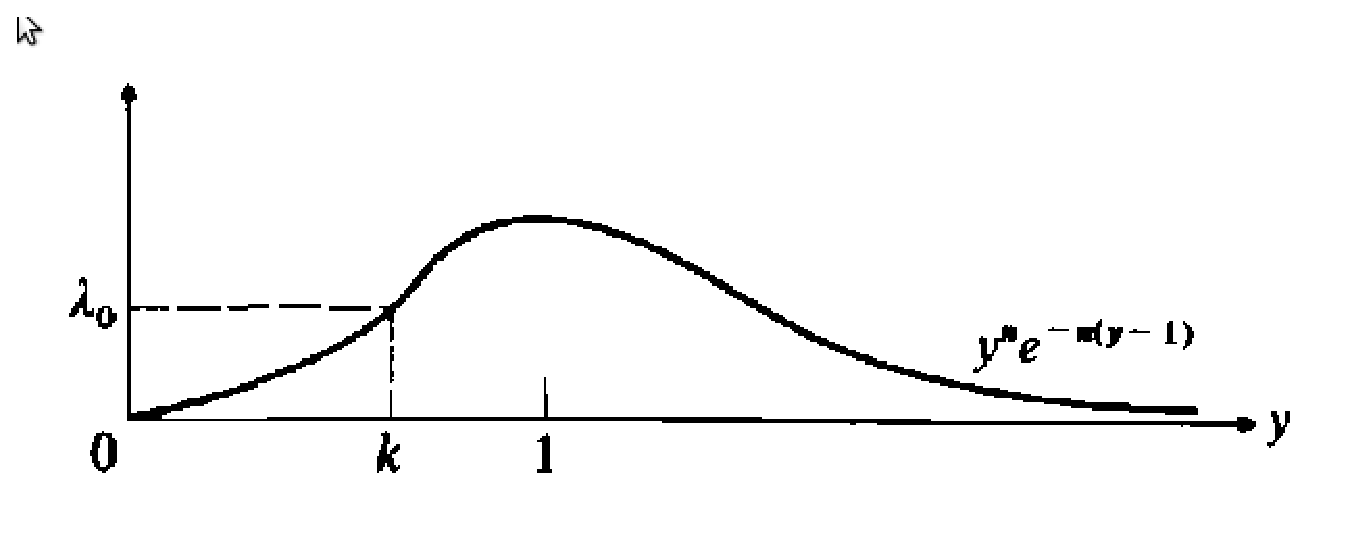
\includegraphics[scale = 0.5]{pictures/example_9_11.eps}
\caption{Funkce charakteristické veličiny}
\label{example_9_11}
\end{figure}

Na závěr uveďme, že vzhledem ke kritériu rozkladu musí obecný věrohodnostní poměrový test záviset pouze na minimální dostatečné statistice.

\subsection{Uniformě nejsilnější test}

\begin{definition}[Uniformě nejsilnější test]
Test $\mathscr{T}^*$ pro $\mathscr{H}_0: \theta \in \overline{\underline{\Theta}}_0$ vs. $\mathscr{H}_1: \theta \in \overline{\underline{\Theta}} - \overline{\underline{\Theta}}_0$ je uniformě nejsilnější test právě tedhy a jen tehdy, jestliže
\begin{enumerate}
\item $\sup_{\theta \in \overline{\underline{\Theta}}_0} \pi_{\mathscr{T}^*}(\theta) = \alpha$\\
\item $\pi_{\mathscr{T}^*}(\theta) \ge \pi_{\mathscr{T}}(\theta)$ pro všechna $\theta \in \overline{\underline{\Theta}} - \overline{\underline{\Theta}}_0$ a libovolný alternativní test $\mathscr{T}$ velikosti menší nebo rovnou $\alpha$.
\end{enumerate}
\end{definition}

Test $\mathscr{T}^*$ je uniformě nejsilnějším testem s velikostí $\alpha$, jestliže mezi všemi ostatními testy s velikostí rovnou nebo menší než $\alpha$ má největší sílu pro všechny alternativní hodnoty $\theta$. Přívlastek ``uniformní'' je váže právě ke ``všem'' alternativním hodnotám $\theta$. Uniformě nejsilnější test pro dané hypotézy nemusí vždy existovat.

\begin{example}
Uvažujme náhodný výběr $X_1, ..., X_n$ z populace $f(x, \theta) = \theta e^{-\theta x}I_{(0, \infty)}(x)$, kde $\overline{\underline{\Theta}} = \{\theta: \theta \ge \theta_0\}$. Pokusme se nalézt uniformě nejsilnější test pro $\mathscr{H}_0: \theta = \theta_0$ vs. $\mathscr{H}_1: \theta > \theta_0$.

Z příkladu (9.7) víme, že pro fixní $\theta_1 > \theta_0$ a   $\mathscr{H}_0: \theta = \theta_0$ vs. $\mathscr{H}_1: \theta = \theta_0$ nejsilnější test zamítne $\mathscr{H}_0$, jestliže $\sum x_i \le k'$, kde $k'$ je dáno řešením rovnice
\begin{equation*}
\alpha = \int_0^{k'} \frac{1}{\Gamma(n)}\theta_0^n x^{n - 1}e^{-\theta_0 x}dx
\end{equation*}
Tento test vyplynul z Neyman-Pearsonovy věty. Vzhledem k tomu, že s vyjímkou podmínky $\theta_1 > \theta_0$ tento test nezávisí na $\theta_1$, zíkali bychom stejný test pro libovolné $\theta_1 > \theta_0$. Proto se jedná o uniformě nejsilnější test.
\end{example}

Následující větu uvádíme bez důkazu.

\begin{theorem}
Uvažujme náhodný výběr $X_1, ..., X_n$ z populace $f(x, \theta)$, kde $\theta \in \overline{\underline{\Theta}}$ a $\overline{\underline{\Theta}}$ je interval. Předpokládejme, že
\begin{equation*}
f(x, \theta) = a(\theta)b(x)e^{c(\theta)d(x)}
\end{equation*}
a definujme statistiku
\begin{equation*}
\mathfrak{t}(x_1, ..., x_n) = \sum_{i = 1}^n d(x_i)
\end{equation*}
\begin{enumerate}
\item Jestliže je $c(\theta)$ monotónní rostoucí funkce v $\theta$ a jestliže existuje $k^*$ takové, že $P_{\theta_0}[\mathfrak{t}(X_1, ..., X_n) > k^*] = \alpha$, pak test $\mathscr{T}^*$ s kritickým regionem $C^* = \{(x_1, ..., x_n): \mathfrak{t}(x_1, ..., x_n) > k^*\}$ je uniformě nejsilnějším testem velikosti $\alpha$ pro $\mathscr{H}_0: \theta \le \theta_0$ vs. $\mathscr{H}_1: \theta > \theta_0$ nebo $\mathscr{H}_0: \theta = \theta_0$ vs. $\mathscr{H}_1: \theta > \theta_0$.
\item Jestliže je $c(\theta)$ monotónní klesající funkce v $\theta$ a jestliže existuje $k^*$ takové, že $P_{\theta_0}[\mathfrak{t}(X_1, ..., X_n) < k^*] = \alpha$, pak test $\mathscr{T}^*$ s kritickým regionem $C^* = \{(x_1, ..., x_n): \mathfrak{t}(x_1, ..., x_n) < k^*\}$ je uniformě nejsilnějším testem velikosti $\alpha$ pro $\mathscr{H}_0: \theta \le \theta_0$ vs. $\mathscr{H}_1: \theta > \theta_0$ nebo $\mathscr{H}_0: \theta = \theta_0$ vs. $\mathscr{H}_1: \theta > \theta_0$.
\end{enumerate}
\end{theorem}

\begin{example}
Uvažujme náhodný výběr $X_1, ..., X_n$ z populace $f(x, \theta) = \theta e^{-\theta x}I_{(0, \infty)}(x)$, kde $\overline{\underline{\Theta}} = \{\theta> \theta > 0\}$. Testované hypotézy mají tvar $\mathscr{H}_0: \theta \le \theta_0$ vs. $\mathscr{H}_1: \theta > \theta_0$. Pravděpodobnostní funkci lze vyjádřit ve tvaru
\begin{equation*}
f(x, \theta) = \theta I_{(0, \infty)}(x)e^{-\theta x} = a(\theta)b(x)e^{c(\theta)d(x)}
\end{equation*}
a proto $\mathfrak{t}(x_1, ..., x_n) = \sum x_i$, $c(\theta) = -\theta$. $c(\theta)$ je monotónní klesající funkce, a proto dle bodu (2) výše uvedené věty uniformě nejsilnější test zamítne $\mathscr{H}_0$ pro $\sum x_i < k^*$, kde $k^*$ je řešením rovnice
\begin{equation*}
\alpha = P_{\theta_0}\left[\sum_{i = 1}^n X_i < k^* \right] = \int_0^{k^*}\frac{1}{\Gamma(n)}\theta_0^n u^{n - 1}e^{-\theta_0 u}du
\end{equation*} 
\end{example}

\begin{definition}[Monotonní věrohodnostní poměr]
O rodině pravděpodobnostních rozdělení $\{f(x, \theta): \theta\ \in \overline{\underline{\Theta}}, \textit{kde} ~ \overline{\underline{\Theta}} ~ \textit{je interval}\}$ říkáme, že mají monotónní věrohodnostní poměr, jestliže existuje statistika $T = \mathfrak{t}(X_1, ..., X_n)$ taková, že poměr
\begin{equation*}
\frac{L(\theta'; x_1, ..., x_n)}{L(\theta''; x_1, ..., x_n)}
\end{equation*}
je buďto nerostoucí funkcí $\mathfrak{t}(x_1, ..., x_n)$ pro každé $\theta' < \theta''$ nebo neklesající funkcí $\mathfrak{t}(x_1, ..., x_n)$ pro každé $\theta' < \theta''$.
\end{definition}

\begin{example}
Jestliže $\{f(x; \theta): \theta \in \overline{\underline{\Theta}}\} = \{\theta e^{-\theta x}I_{(0, \infty)}(x): \theta > 0\}$, pak
\begin{equation*}
\frac{L(\theta'; x_1, ..., x_n)}{L(\theta''; x_1, ..., x_n)} = \frac{(\theta')^n e^{-\theta' \sum_{i = 1}^n x_i}}{(\theta'')^n e^{-\theta'' \sum_{i = 1}^n x_i}} = \left(\frac{\theta'}{\theta''}\right)^n e^{-(\theta' - \theta'')\sum_{i = 1}^n x_i}
\end{equation*}
což je monotónní rostoucí funkce v $\sum x_i$.
\end{example}

\begin{example}
Jestliže $\{f(x; \theta): \theta \in \overline{\underline{\Theta}}\} = \{(1/\theta)I_{(0, \infty)}(x): \theta > 0\}$, pak
\begin{multline*}
\frac{L(\theta'; x_1, ..., x_n)}{L(\theta''; x_1, ..., x_n)} = \frac{\left(\frac{1}{\theta'}\right)^n \prod_{i = 1}^n I_{(0, \theta')}(x_i)}{\left(\frac{1}{\theta''}\right)^n \prod_{i = 1}^n I_{(0, \theta'')}(x_i)}\\
=
\begin{cases}
\left(\frac{\theta''}{\theta'}\right)^n ~ \textit{pro} ~ 0 < y_n < \theta'\\
0 ~ \textit{pro} ~ \theta' \le y_n < \theta''
\end{cases}
\end{multline*}
což je monotónní nerostoucí funkce v $y_n = \max(x_1, ..., x_n)$. Připomeňme, že $y_n$ nemůže padnout mimo interval $(0, \theta'')$, jestliže $\theta$ nabývá hodnoty $\theta'$ nebo $\theta''$.
\end{example}

Následující větu uvádíme bez důkazu.

\begin{theorem}
Uvažujme náhodný výběr $X_1, ..., X_n$ z populace $f(x; \theta)$, kde $\overline{\underline{\Theta}}$ představuje interval. Předpokládejme, že rodina pravděpodobnostních rozdělení $\{f(x;\theta): \theta \in \overline{\underline{\Theta}}\}$ má monotónní věrohodnostní poměr pro statistiku $\mathfrak{t}(X_1, ..., X_n)$.
\begin{enumerate}
\item Jestliže je monotónní věrohodnostní poměr neklesající v $\mathfrak{t}(x_1, ..., x_n)$ a jestliže existuje $k^*$ takové, že $P_{\theta_0}[\mathfrak{t}(X_1, ..., X_n) < k^*] = \alpha$, pak je test odpovídající kritickému regionu $C^* = \{(x_1, ..., x_n): \mathfrak{t}(x_1, ..., x_n) < k^*\}$ uniformě nejsilnější test síly $\alpha$ pro $\mathscr{H}_0: \theta \le \theta_0$ vs. $\mathscr{H}_1: \theta > \theta_0$.
\item Jestliže je monotónní věrohodnostní poměr nerostoucí v $\mathfrak{t}(x_1, ..., x_n)$ a jestliže existuje $k^*$ takové, že $P_{\theta_0}[\mathfrak{t}(X_1, ..., X_n) > k^*] = \alpha$, pak je test odpovídající kritickému regionu $C^* = \{(x_1, ..., x_n): \mathfrak{t}(x_1, ..., x_n) > k^*\}$ uniformě nejsilnější test síly $\alpha$ pro $\mathscr{H}_0: \theta \le \theta_0$ vs. $\mathscr{H}_1: \theta > \theta_0$.
\end{enumerate}
\end{theorem}

\begin{example}
Uvažujme náhodný výběr $X_1, ..., X_n$ z populace $f(x; \theta) = \frac{1}{\theta}I_{(0, \theta)}(x)$, kde $\theta > 0$ a hypotézy $\mathscr{H}_0: \theta \le \theta_0$ vs. $\mathscr{H}_1: \theta > \theta_0$. Z předchozího příkladu víme, že toto pravděpodobnostní rozdělení má monotónní nerostoucí věrohodnostní poměr pro $\mathscr{t}(x_1, ..., x_n) = y_n = \max(x_1, ..., x_n)$. Dle bodu (2) výše uvedené věty je uniformě nejsilnější test velikosti $\alpha$ definován jako zamítnutí $\mathscr{H}_0$, jestliže $y_n > k^*$, kde $k^*$ je řešením rovnice
\begin{equation*}
\alpha = P_{\theta_0}[Y_n > k^*] = \int_{k^*}^{\theta_0}n \left(\frac{y}{\theta_0}\right)^{n - 1} \frac{dy}{\theta_0} = \frac{1}{\theta_0^n}[\theta_0^n - (k^*)^n] = 1 - \left(\frac{k^*}{\theta_0}\right)^n
\end{equation*}
což implikuje $k^* = \theta_0 \sqrt[n]{1 - \alpha}$.
\end{example}

Závěrem uveďme následující tři poznámky. Za prvé, jak ve větě (9.5) tak ve větě (9.6) je nulová hypotéza formulována jako $\theta \le \theta_0$. Jestliže by nulová hypotéza byla formulována jako $\theta \ge \theta_0$, zůstaly by obě věty v platnosti, pokud bychom obrátily nerovnosti, které definují kritický region. Za druhé, věta (9.5) je důsledkem věty (9.6). Za třetí, obě věty uvažují pouze jednostranné hypotézy.

\subsection{Nezkreslený test}

V řadě případů uniformě nejsilnější test neexistuje. V takovém případě můžeme soubor testů omezit a následně nalézt uniformě nejsilnější test na této omezené množině. Tímto se dostáváme ke konceptu nezkresleného testu.

\begin{definition}[Nezkreslený test]
Test $\mathscr{T}$ hypotéz $\mathscr{H}_0: \theta \in \overline{\underline{\Theta}}_0$ vs. $\mathscr{H}_1: \theta \in \overline{\underline{\Theta}}_1$ je nezkreslený test, jestliže
\begin{equation*}
\sup_{\theta \in \overline{\underline{\Theta}}_0} \pi_{\mathscr{T}}(\theta) \le \inf_{\theta \in \overline{\underline{\Theta}}_1}\pi_{\mathscr{T}}(\theta)
\end{equation*}
\end{definition}

V případě nezkresleného testu je tedy pravděpodobnost zamítnutí nepravdivé $\mathscr{H}_0$ přinejmenším stejně velká jako pravděpodobnost zamítnutí pravdivé $\mathscr{H}_0$. Jestliže v rámci takto omezené množiny testů existuje test, který je uniformě nejsilnější, pak se jedná o uniformě nejsilnější nezkreslený test. Pro nalezení uniformě nejsilnějšího nezkresleného testu byla vyvinuta poměrně složitá teorie, která však přesahuje záběr této knihy.

\subsection{Metody pro nalézání testů}

V rámci testu testujeme nulovou hypotézu $\mathscr{H}_0$ proti alternativní hypotéze $\mathscr{H}_1$. Uvažujme stastistiku, která pro obě hypotézy chová ``odlišně'', a pokusme se využít toto odlišné chování pro definici testu. Jako ilustraci uvažujme testování $\mathscr{H}_0: \theta \le \theta_0$ vs. $\mathscr{H}_1: \theta > \theta_1$, kde náhodný výběr $X_1, ..., X_n$ pochází z $f(x; \theta) = \phi_{\theta, 1}(x)$. Statistika $\overline{X}$ sleduje normální rozdělení se střední hodnotou $\theta$ a rozptylem $1/n$. Lze tedy očekávat, že $\overline{X}$ bude menší pro pravdivé $\mathscr{H}_0$ a větší pro pravdivé $\mathscr{H}_1$ - statistika $\overline{X}$ se tak chová odlišně pro nulovou a alternativní hypotézu. Rozumným testem se tedy zdá zamítnutí $\mathscr{H}_0$, je-li $\overline{X} > k$, kde $k$ je dáno velikostí testu\footnote{Z předchozí kapitoly víme, že takovýto test je uniformě nejsilnější.}.

Klíčem této techniky je tedy nalezení statistiky, která vykazuje ``odlišné'' chování pro nulovou a alternativní hypotézu. Jestliže existuje dostatečná statistika, pak se jedná o přirozeného kandidáta. V opačné případě je možné použít vhodnou funkci odhadu\footnote{Např. funkci odhadu založenou na metodě maximální věrohodnosti.}. Ve výše uvedeném případě tuto funkci plní $\overline{X}$, což zároveň dostatečná statistika a funkce odhadu parametru $\theta$ založená na metodě maximální věrohodnosti.

\begin{example}
Uvažujme náhodný výběr $X_1, ..., X_n$ z Poissonova rozdělení se střední hodnotou $\theta$. Testujeme $\mathscr{H}_0: \theta = \theta_0$ vs. $\mathscr{H}_1: \theta \neq \theta_1$. Předpokládejme $n = 10$ a $\theta_1 = 1$.

Víme, že $\overline{X}$ je funkce odhadu pro $\theta$ založená na metodě maximální věrohodnosti. To znamená, že $\overline{X}$ bude mít tendenci se nacházet v okolí $\theta_0$, jestliže je $\mathscr{H}_0$ pravdivá. Přirozená formulace testu tedy zní: ``Přijmi $\mathscr{H}_0$, jestliže $c_1 < \overline{x} < c_2$'', kde $c_1$ a $c_2$ jsou zvoleny tak, aby měl test požadovanou velikost. Např. test ``přijmi $\mathscr{H}_0$, jestliže $0.4 < \overline{x} < 1.6$'' má velikost
\begin{multline*}
1 - P_{\theta = 1}[0.4 < \overline{X} < 1.6] = 1 - P_{\theta = 1}[4 < \sum_{i = 1}^{10} X_i < 16]\\
= 1 - \sum_{j = 5}^{15}\frac{e^{-10}10^j}{j!} \approx 0.078
\end{multline*}
\end{example}

Test, který je běžně používán v praxi, testuje $\mathscr{H}_0: \theta = \theta_0$ vs. $\mathscr{H}_1: \theta \neq \theta_0$. Pro ilustraci předpokládejme, že $\theta$ je rozdílem výnosů dvou odrůd pšenice. Na první pohled by se mohlo zdát, že kandidátem na vhodný test je $\mathscr{H}_0: \theta = 0$ vs. $\mathscr{H}_1: \theta \neq 0$, který testuje, zda-li existuje rozdíl ve výnosech obou odrůd. Nicméně $\theta$ je spojitá veličina, a proto není možné, aby nabývala právě hodnoty nula. Jako vhodnější se proto jeví test $\mathscr{H}_0: \theta_1 le \theta \le \theta_2$ vs. $\mathscr{H}_1: \theta < \theta_1 ~ \textit{nebo} ~ \theta > \theta_2$. Nalézt odpovídající uniformě nejsilnější test může být složité či dokonce nemožné. Nicméně jestliže $f(x; \theta)$ je pravděpodobnostním rozdělením s jedním parametrem, pak lze pro konstrukci testu použít funkci odhadu $\hat{\Theta}$ založenou na metodě maximální věrohodnosti a síla tohoto testu je pak porovnána s ideální funkcí charakteristické veličiny testu velikosti $\alpha$. Pro některá pravděpodobnostní rozdělení lze použít test, který zamítne $\theta_0$, jestliže se $\hat{\theta}$ nenachází v určitém intervalu $(c_1, c_2)$, kde $c_1$ a $c_2$ mohou být vybrána tak, aby platilo
\begin{equation*}
\int_{c_1}^{c_2} f_{\hat{\Theta}}(\hat{\theta}; \theta_1)d \hat{\theta} = \int_{c_1}^{c_2} f_{\hat{\Theta}}(\hat{\theta}; \theta_2)d \hat{\theta} = 1 - \alpha
\end{equation*}
kde $f_{\hat{\Theta}}(\hat{\theta}, \theta)$ je pravděpodnostní funkce $\hat{\Theta}$ pro parametr $\theta$. Odpovídající funkce charakteristické veličiny je pak
\begin{equation*}
\pi(\theta) = 1 - \int_{c_1}^{c_2}f_{\hat{\Theta}}(\hat{\theta}; \theta) d \hat{\theta} ~ \textit{pro} ~ \theta \in \overline{\underline{\Theta}}
\end{equation*}
Tuto funkci charakteristické veličiny je možné porovnat s ideální funkcí charakteristické veličiny a pokud její odchylka nepřesahuje přijatelnou mez, může být příslušný test použit, i když se nejedná o uniformě nejsilnější test.

\begin{example}
Uvažujme náhodný výběr $X_1, ..., X_n$ z populace $\phi_{\theta, 1}(x)$. Testujme $\mathscr{H}_0: 1 \le \theta \le 2$ vs. $\mathscr{H}_1: \theta < 1 ~ \textit{nebo} ~ \theta > 2$.

Víme, že $\overline{X}$ je funkce odhadu pro $\theta$ dle metody maximální věrohodnosti. Tato statistika sleduje normální rozdělení se střední hodnotou $\theta$ a rozptylem $1/n$. Naším cílem je nalézt $c_1$ a $c_2$ takové, aby platilo
\begin{equation*}
1 - \alpha = \int_{c_1}^{c_2} \phi_{1, 1/n}(x)dx = \int_{c_1}^{c_2} \phi_{2, 1/n}(x)dx
\end{equation*}
tj.
\begin{equation*}
\Phi\left(\frac{c_2 - 1}{\sqrt{1/n}}\right) - \Phi\left(\frac{c_1 - 1}{\sqrt{1/n}}\right) = \Phi\left(\frac{c_2 - 2}{\sqrt{1/n}}\right) - \Phi\left(\frac{c_1 - 2}{\sqrt{1/n}}\right) = 1 - \alpha
\end{equation*}
Jak je patrné z obrázku (\ref{example_9_18a}), platí $c_1 = \frac{3}{2} - d$ a $c_2 = \frac{3}{2} + d$, kde $d$ je dáno
\begin{equation*}
\Phi \left(\frac{d + \frac{1}{2}}{\sqrt{1/n}}\right) - \left(\frac{\frac{1}{2} - d}{\sqrt{1/n}}\right) = 1 - \alpha
\end{equation*}
Jestliže, např. $\alpha = 0.05$ a $n = 16$, pak $d \approx 0.911$, $c_1 \approx 0.589$ a $c_2 \approx 2.411$. Funkce charakteristické veličiny je
\begin{equation*}
\pi(\theta) = 1 - P_{\theta}[c_1 < \overline{X} < c_2] = 1 - P_{\theta}[0.589 < \overline{X} < 2.411]
\end{equation*}
a je ilustrována obrázkem  (\ref{example_9_18b}).
\end{example}

\begin{figure}[htp]
\centering
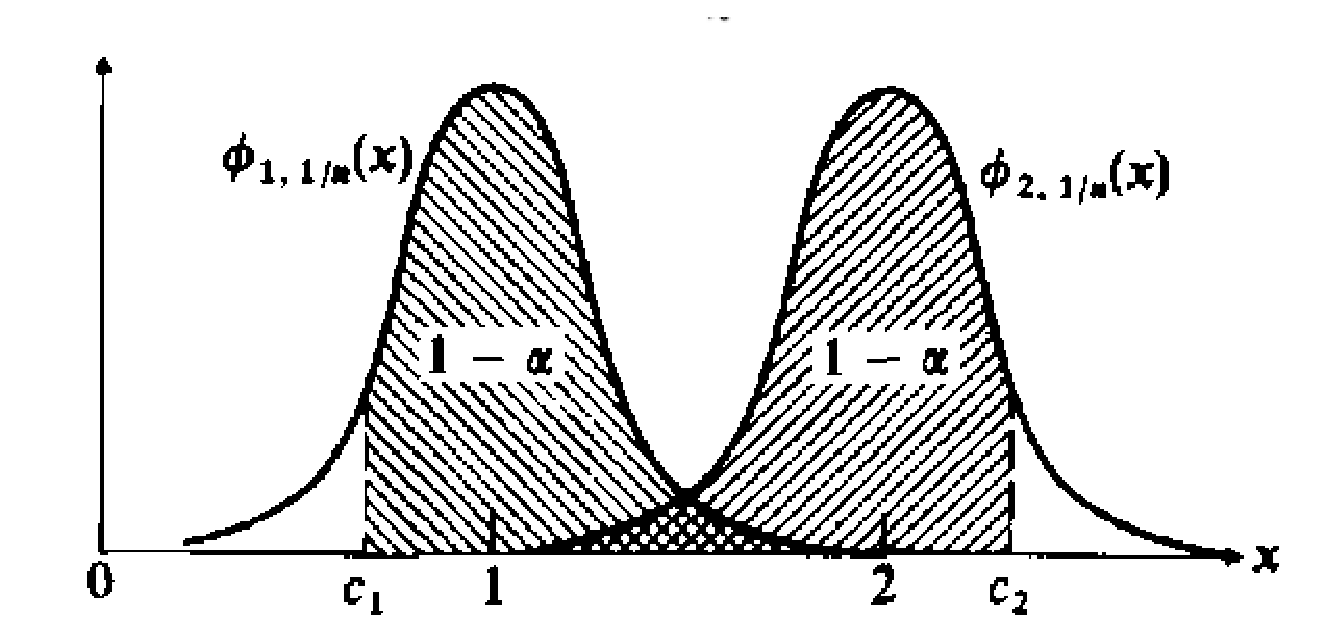
\includegraphics[scale = 0.5]{pictures/example_9_18a.eps}
\caption{Ilustrační obrázek}
\label{example_9_18a}
\end{figure}

\begin{figure}[htp]
\centering
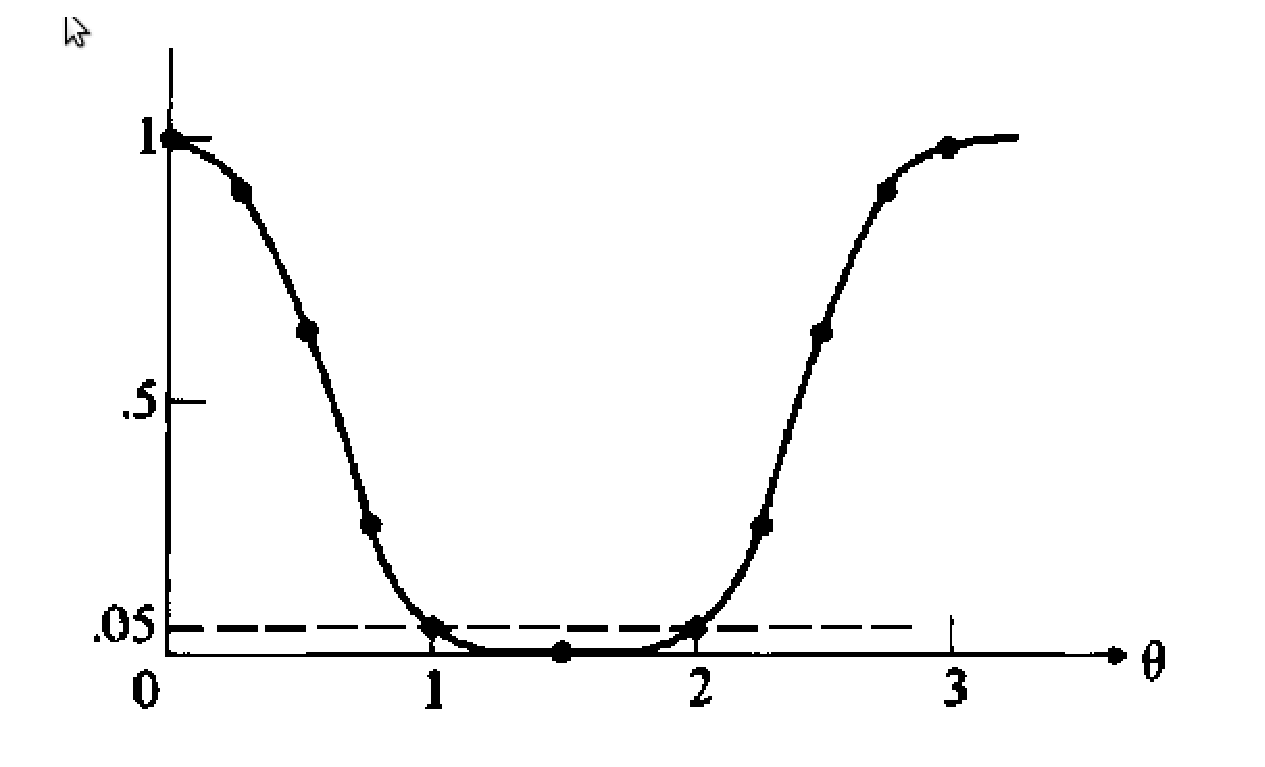
\includegraphics[scale = 0.5]{pictures/example_9_18b.eps}
\caption{Ilustrační obrázek}
\label{example_9_18b}
\end{figure}

\section{Testování hypotéz - výběr z normálního rozdělení}

\subsection{Testování středních hodnot}

\subsubsection{$\mathscr{H}_0: \mu \le \mu_0$ vs. $\mathscr{H}_1: \mu > \mu_0$}

Nejprve předpokládejme, že známe $\sigma^2$. Normální pravděpodobnostní rozdělení
\begin{equation*}
f(x, \theta) = \phi_{\mu, \sigma^2}(x) = \frac{1}{\sqrt{2\pi} \sigma}e^{-\frac{1}{2}\left(\frac{x - \mu}{\sigma}\right)} = \frac{1}{\sqrt{2\pi}\sigma}e^{-\frac{1}{2}\left(\frac{\mu}{\sigma}\right)^2}e^{-\frac{1}{2}\left(\frac{x}{\sigma}\right)^2}e^{\frac{\mu}{\sigma}x}
\end{equation*}
je člen rodiny exponenciálních rozdělení s
\begin{equation*}
a(\mu) = \frac{1}{\sqrt{2 \pi}\sigma}e^{-\frac{1}{2}\left(\frac{\mu}{\sigma}\right)^2}, ~ b(x) = e^{-\frac{1}{2}\left(\frac{x}{\sigma}\right)^2}, ~ c(\mu) = \frac{\mu}{\sigma} ~ a ~ d(x) = x
\end{equation*}
Podmínky věty (9.5) jsou splněny, a proto uniformě nejsilnější test existuje a zavrhuje $\mathscr{H}_0$ pro $\mathfrak{t}(x_1, ..., x_n) = \sum x_i > k^*$, kde $k^*$ je řešením $P_{\mu_0}[\sum X_i > k^*] = \alpha$. Protože $\alpha = P_{\mu_0}[\sum X_i > k^*] = 1 - \Phi\left(\frac{k^* - n \mu_0}{\sqrt{n} \sigma}\right)$, tak $\frac{k^* - n \mu_0}{\sqrt{n} \sigma} = z_{1 - \alpha}$, kde $z_{1 - \alpha}$ je $(1 - \alpha)$-tý kvantil normovaného normálního rozdělení. Test tedy zamítne $\mathscr{H}_0$, jestliže $\sum x_i > n \mu_0 + \sqrt{n}\sigma z_{1 - \alpha}$ neboli $\overline{x} > \mu_0 + \frac{\sigma}{\sqrt{n}}z_{1 - \alpha}$.

Jestliže je $\sigma^2$ neznáme, pak je testování $\mathscr{H}_0: \mu \le \mu_0$ vs. $\mathscr{H}_1: \mu > \mu_0$ ekvivalentní testování $\mathscr{H}_0: \theta \in \overline{\underline{\Theta}}_0$ vs. $\mathscr{H}_1: \theta \notin \mu_0$, kde $\theta = (\mu, \sigma^2)$, $\overline{\underline{\Theta}} = \{(\mu, \sigma^2): -\infty < \mu < \infty; \sigma^2 > 0\}$  a $\overline{\underline{\Theta}}_0 = \{(\mu, \sigma^2): \mu \le \mu_0; \sigma^2 > 0\}$. Pro formulaci testu můžeme (a) použít obecný věrohodnostní poměr nebo (b) nalézt statistiku, která se pro obě hypotézy chová ``odlišně'' a založit na ní test. Příkladem takovéto statistiky je $T = \frac{\overline{X} - \mu_0}{S / \sqrt{n}}$, kde $\overline{X}$ je střední hodnota výběru a $S^2$ je výběrový rozptyl. Protože $T$ bude větší pro $\mu > \mu_0$ než pro $\mu \le \mu_0$, bude test zavrhovat $\mathscr{H}_0$ pro vysoké hodnoty $T$, tj. zamítne $\mathscr{H}_0$, jestliže $T > k$. Jestliže $\mu = \mu_0$, pak $T$ sleduje studentovo rozdělení s $n - 1$ stupni volnosti. $k$ je tak možné získat z $\alpha = P_{\mu_0}[T > k]$, což implikuje $k = t_{1 - \alpha}(n-1)$, tj. $k$ je rovno kvantilu $(1 - \alpha)$ studentova rozdělení s $(n - 1)$ stupni volnosti. Lze dokázat, že takto odvozený test je zároveň testem velikosti $\alpha$ založeným na obecném věrohodnostním poměru.

\subsubsection{$\mathscr{H}_0: \mu = \mu_0$ vs. $\mathscr{H}_1: \mu \neq \mu_0$}

Jestliže známe $\sigma^2$, pak je $\left(\overline{X} - z_{(1 + \gamma)/2}(\sigma / \sqrt{n}), \overline{X} + z_{(1 + \gamma)/2}(\sigma / \sqrt{n})\right)$ je 100$\gamma$ procentní interval spolehlivosti pro $\mu$, kde $z_{(1 + \gamma)/2}$ je $(1 + \gamma)/2$ procentní kvantil normovaného normálního rozdělení. Test pak zamítne $\mathscr{H}_0$, jestliže tento interval nezahrnuje $\mu_0$. Takto definovaný test má navíc velikost $1 - \gamma$, protože
\begin{equation*}
P_{\mu = \mu_0}\left[\overline{X} - z_{(1 + \gamma)/2}\frac{\sigma}{\sqrt{n}} < \mu_0 < \overline{X} + z_{(1 + \gamma)/ 2} \frac{\sigma}{\sqrt{n}}\right] = \gamma
\end{equation*}

Jestliže je $\sigma^2$ neznámé, pak lze odvodit test podobný výše uvedenému, který vychází z 100$\gamma$ procentního intervalu spolehlivosti
\begin{equation*}
\left(\overline{X} - t_{(1 + \gamma)/2}(n - 1)\frac{S}{\sqrt{n}}, \overline{X} + t_{(1 + \gamma)/2}(n - 1) \frac{S}{\sqrt{n}}\right)
\end{equation*}
Pokusme se však nalézt test založený na obecném věrohodnostním poměru. Funkce maximální věrohodnosti má tvar
\begin{equation*}
L(\mu, \sigma^2; x_1, ..., x_n) = \left(\frac{1}{\sqrt{2 \pi} \sigma}\right)^n e^{-\frac{1}{2}\sum_{i = 1}^n \left(\frac{x_i - \mu}{\sigma}\right)^2}
\end{equation*}
$\overline{\underline{\Theta}}_0 = \{(\mu, \sigma^2): \mu = \mu_0; \sigma^2 > 0\}$ a $\overline{\underline{\Theta}} = \{(\mu, \sigma^2): -\infty < \mu < \infty; \sigma^2 > 0\}$. Víme, že hodnoty pro $\mu$ a $\sigma^2$, které maximalizují $L(\mu, \sigma^2; x_1, ..., x_n)$ nad $\overline{\underline{\Theta}}$, jsou $\hat{\mu} = \overline{x}$ a $\hat{\sigma}^2 = \frac{\sum_{i = 1}^n (x_i - \overline{x})^2}{n}$, proto
\begin{equation*}
\sup_{\overline{\underline{\Theta}}} L(\mu, \sigma^2; x_1, ..., x_n) = \left(\frac{n}{2 \pi \sum_{i = 1}^n (x_i - \overline{x})^2}\right)^{n/2}e^{-n/2}
\end{equation*}
Abychom maximalizovali $L(\mu, \sigma^2; x_1, ..., x_n)$ nad $\overline{\underline{\Theta}}_0$, dosaďme $\mu = \mu_0$. Jediným neznámým parametrem tak zůstává $\sigma^2$, který maximalizuje $L(\mu, \sigma^2; x_1, ..., x_n)$ pro $\frac{\sum (x_i - \mu_0)^2}{n}$, čímž získáváme
\begin{equation*}
\sup_{\overline{\underline{\Theta}}_0} L(\mu, \sigma^2; x_1, ..., x_n) = \left(\frac{n}{2 \pi \sum_{i = 1}^n (x_i - \mu_0)^2}\right)^{n/2}e^{-n/2}
\end{equation*}
Obecný věrohodností poměr je tak
\begin{gather*}
\lambda = \left(\frac{\sum_{i = 1}^n (x_i - \overline{x})^2}{\sum_{i = 1}^n (x_i - \mu_0)^2}\right)^{n/2} = \left(\frac{\sum_{i = 1}^n (x_i - \overline{x})^2}{\sum_{i = 1}^n (x_i - \overline{x} + \overline{x} + \mu_0)^2}\right)^{n/2}\\
\left(\frac{\sum_{i = 1}^n (x_i - \overline{x})^2}{\sum_{i = 1}^n (x_i - \overline{x})^2 + n(\overline{x} - \mu)^2}\right)^{n/2} = \left(\frac{1}{1 + n(\overline{x} - \mu_0)^2 / \sum_{i = 1}^n(x_i - \overline{x})^2}\right)^{n/2}
\end{gather*}
Všimněme si, že $\lambda$ je monotónní funkcí pro statistiku
\begin{equation*}
t^2 = \mathfrak{t}^2(x_1, ..., x_n) - \frac{n(n - 1)(\overline{x} - \mu_0)^2}{\sum_{i = 1}^n (x_i - \overline{x})^2} = \left(\frac{\overline{x} - \mu_0}{\sqrt{\sum_{i = 1}^n (x_i - \overline{x})^2 / (n-1)n}}\right)^2
\end{equation*}
a proto je kritický region ve tvaru $\lambda \le \lambda_0$ ekvivalentní kritickému regionu ve tvaru $\mathfrak{t}^2(x_1, ..., x_n) \ge k^2$. Test založený obecném věrohodnostním poměru tak zamítne $\mathscr{H}_0$, jestliže
\begin{equation*}
T^2 = \left(\frac{\overline{X} - \mu_0}{S / \sqrt{n}}\right)^2 \ge k^2
\end{equation*}
neboli přijme $\mathscr{H}_0$, jestliže $-k < T < k$. Protože $T$ sleduje studentovo rozdělení s $n - 1$ stupni volnosti pro $\mu = \mu_0$, je $k$ vybráno tak, aby splňovalo
\begin{equation*}
\int_{-k}^k f_T(t; n-1)dt = 1 - \alpha
\end{equation*}
kde $\alpha$ je požadovaná velikost testu. To znamená, že $k$ je rovno $t_{(1 - \alpha)/2}(n - 1)$, tj. kvantilu $(1 - \alpha)/2$ studentova rozdělení s $n - 1$ stupni volnosti. Takto odvozený test se shoduje s testem založeném na intervalu spolehlivosti, který jsme definovali na začátku jako
\begin{equation*}
\left(\overline{X} - t_{(1 + \gamma) / 2}(n - 1)\frac{S}{\sqrt{n}}, \overline{X} + t_{(1 + \gamma)/2}(n - 1)\frac{S}{\sqrt{n}}\right)
\end{equation*}
kde $\gamma = 1 - \alpha$. Bez důkazu uveďme, že tento test je také uniformě nejsilnějším testem.

\subsubsection{Ostatní případy}

Ve výše uvedeném textu jsme odvodili test střední hodnoty normálního rozdělení pro jednostrané i oboustranné hypotézy. Jednostrannou nulovou hypotézu $\mu \le \mu_0$ lze obrátit a získat příslušný test. Je možné definovat také další typy hypotéz, jako např. $\mathscr{H}_0: \mu_1 \le \mu \le \mu_2$ vs. $\mathscr{H}_1: \mu < \mu_1 ~ \textit{nebo} ~ \mu > \mu_2$.

\subsection{Testování rozptylu}

\subsubsection{$\mathscr{H}_0: \sigma^2 \le \sigma_0^2$ vs. $\sigma^2 > \sigma_0^2$}

Předpokládejme, že $\mu$ je známo. Pak je parametrický prostor reprezentovaný intervalem. Námi uvažovaný test je jednostranný, a proto máme naději nalézt uniformě nejsilnější test velikosti $\alpha$. Pravděpodobnostní funkce normálního rozdělení
\begin{equation*}
f(x; \theta) = f(x; \sigma^2) = \frac{1}{\sqrt{2 \pi} \sigma}e^{-\frac{1}{2 \sigma^2}(x - \mu)^2}
\end{equation*}
je člen rodiny exponenciálních rozdělení s $a(\sigma^2) = \frac{1}{\sqrt{2 \pi} \sigma}$, $b(x) = 1$, $c(\sigma^2) = -\frac{1}{2}\sigma^2$ a $d(x) = (x - \mu)^2$. $c(\sigma^2)$ je monotónní rostoucí funkce v $\sigma^2$, a proto dle věty (9.5) je test s kritickým regionem $\{(x_1, ..., x_n): \sum (x_i - \mu)^2 > k^*\}$ uniformě nejsilnějším testem velikosti $\alpha$, přičemž $k^*$ je dáno rovnicí $P_{\sigma^2 = \sigma_0^2}[\sum (X_i - \mu)^2 > k^*] = \alpha$. To implikuje $k^* = \sigma_0^2 \chi_{1 - \alpha}^2(n)$, kde $\chi_{1 - \alpha}^2(n)$ je $1 - \alpha$ procentní kvantil chi-kvadrát rozdělení s $n$ stupni volnosti.

Jestliže $\mu$ není známé, lze test odvodit s pomocí statistiky $V = \frac{\sum(X_i - \overline{X})}{\sigma_0^2}$. Statistika $V$ bude nabývat vysokých hodnot pro $\sigma^2 > \sigma_0^2$, a proto test bude zamítat $\mathscr{H}_0$ pro vysoká $V$. Jestliže $\sigma^2 = \sigma_0^2$, pak bude $V$ sledovat chi-kvadrát rozdělení s $n - 1$ stupni volnosti a $P_{\sigma^2 = \sigma_0^2}[V > \chi_{1 - \alpha}^2(n - 1)] = \alpha$, kde $\chi_{1 - \alpha}^2(n - 1)$ je $(1 - \alpha)$ procentní kvantil chi-kvadrát rozdělení s $n - 1$ stupni volnosti. Lze dokázat, že test, který zamítne $\mathscr{H}_0$ pro $\frac{(X_i - \overline{X})^2}{\sigma_0^2} > \chi_{1 - \alpha}^2(n - 1)$, je také testem velikosti $\alpha$ založeným na obecném věrohodnostním poměru.

\subsubsection{$\mathscr{H}_0: \sigma^2 = \sigma_0^2$ vs. $\sigma^2 \neq \sigma_0^2$}

Vynechme situaci, kdy je $\mu$ známo a zaměřme se na situaci, kdy $\mu$ neznáme. V tomto případě je $\overline{\underline{\Theta}}_0 = \{(\mu, \sigma): - \infty < \mu < \infty; \sigma^2 = \sigma_0^2 \}$. Pokusme se nalézt test velikosti $\alpha$ s využitím metody intervalu spolehlivosti. Z kapitoly (8.2.2) víme, že 100$\gamma$ procentní interval spolehlivosti pro $\sigma^2$ je definován jako
\begin{equation*}
\left(\frac{(n - 1)S^2}{q_2}, \frac{(n - 1)S^2}{q_1}\right)
\end{equation*}
kde $q_1$ a $q_2$ jsou kvantily chi-kvadrát rozdělení $f_Q(q; n - 1)$ s $n - 1$ stupni volnosti, kde
\begin{equation*}
\int_{q_1}^{q_2} f_Q(q; n - 1)dq = \gamma
\end{equation*}
Test velikosti $\alpha = 1 - \gamma$ pak přijme $\mathscr{H}_0$, jestliže $\sigma_0^2$ je obsaženo ve výše uvedeném intervalu. Lze dokázat, že tento test odpovídá testu založeném na obecném věrohodnostním poměru.

\subsection{Test několika středních hodnot}

\subsubsection{Test dvou středních hodnot}

Uvažujme dvě vzájemně nezávislé populace, které sledují normální rozdělení - jednu se střední hodnotou $\mu_1$ a rozptylem $\sigma_1^2$ a druhou se střední hodnotou $\mu_2$ a rozptylem $\sigma_2^2$. Testujme hypotézy $\mathscr{H}_0: \mu_1 = \mu_2, \sigma_1^2 > 0, \sigma_2^2 > 0$ vs. $\mathscr{H}_1: \mu_1 \neq \mu_2, \sigma_1^2 > 0, \sigma_2^2 > 0$. Parametrický prostor $\overline{\underline{\Theta}}$ je tedy čtyřrozměrný a příslušné sdružené pravděpodobnostní rozdělení je definováno skrze $(\mu_1, \mu_2, \sigma_1^2, \sigma_2^2)$. Podprostor $\overline{\underline{H}}_0$ je pak pouze třírozměrný, protože $\mu_1 = \mu_2 = \mu$. Uvažujme náhodný výběr $X_{11}, ..., X_{1n_1}$ z první a náhodný výběr  $X_{21}, ..., X_{2n_2}$ z druhé populace. Funkce věrohodnosti je pak definována jako
\begin{multline*}
L(\mu_1, \mu_2, \sigma_1^2, \sigma_2^2; x_{11}, ..., x_{1n_1}, x_{21}, ..., x_{2n_2}) = L\\
= \left(\frac{1}{2\pi \sigma_1^2}\right)^{n_1/2}e^{-\frac{1}{2}\sum_{i = 1}^n \left(\frac{x_{1i} - \mu_1}{\sigma_1}\right)^2} \left(\frac{1}{2\pi \sigma_2^2}\right)^{n_2/2}e^{-\frac{1}{2}\sum_{j = 1}^n \left(\frac{x_{2j} - \mu_2}{\sigma_2}\right)^2}
\end{multline*}
a její maximum nad $\overline{\underline{\Theta}}$ je
\begin{equation*}
\sup_{\overline{\underline{\Theta}}}L = \left(\frac{n_1}{2 \pi \sum_{i = 1}^{n_1}(x_{1i} - \overline{x}_1)^2}\right)^{n_1/2} \left(\frac{n_2}{2 \pi \sum_{j = 1}^{n_2}(x_{2j} - \overline{x}_2)^2}\right)^{n_2/2}e^{-n_1/2}e^{-n_2/2}
\end{equation*}
Jestliže použijeme $\mu_1 = \mu_2 = \mu$ a pokusíme se maximalizovat $L$ vzhledem k $\mu, \sigma_1^2$ a $\sigma_2^2$, zjistíme, že odhad $\mu$ má charakter kořene polynomu třetího řádu a že se jedná o poměrně složitou funkci. To znamená, že také obecný věrohodnostní poměr $\lambda$ je složitou funkcí, která navíc obsahuje podíl rozptylů $\sigma_1^2$ a $\sigma_2^2$ a její pravděpodobnostní funkce je velmi náročná na odvození. Je tedy nemožné analyticky odvodit kritický region $0 < \lambda < k$ pro danou pravděpodobnost chyby typu I, protože poměr rozptylů uvažovaných populací není znám. Kořen polynomu třetího řádu je možné vypočíst numericky, což nám následně umožní výpočet $\lambda$. Pro velké populace navíc, jak si ukážeme v kapitole (9.5), platí, že $- \ln(\Lambda)$ přibližně sleduje chi-kvadrát rozdělení s jedním stupněm volnosti. To nám umožní konstrukci testu, který zamítne $\mathscr{H}_0$ pro velká $-2 \ln(\lambda)$.

Jestliže mají obě uvažované populace shodný rozptyl, problematika se značně zjednoduší. Parametrický prostor $\overline{\underline{\Theta}}$ se stává třírozměrným se souřadnicemi $(\mu_1, \mu_2, \sigma^2)$ a parametrický prostor $\overline{\underline{\Theta}}_0$ dvourozměrným se souřadnicemi $(\mu, \sigma^2)$. Pro $\overline{\underline{\Theta}}$ jsou odhady pro $\mu_1, \mu_2$ a $\sigma^2$ dány $\overline{x}_1$, $\overline{x}_2$ a $\frac{1}{n_1 + n_2}\left(\sum_{i = 1}^{n_1}(x_{1i} - \overline{x}_1)^2 + \sum_{i = 1}^{n_2}(x_{2j} - \overline{x}_2)^2\right)$, a proto
\begin{equation*}
\sup_{\overline{\underline{\Theta}}}L = \left(\frac{n_1 + n_2}{2 \pi \left(\sum_{i = 1}^{n_1} (x_{1i} - \overline{x}_1)^2 + \sum_{j = 1}^{n_2}(x_{2j} - \overline{x}_2)^2\right)}\right)^{(n_1 + n_2)/2}e^{-(n_1 + n_2)/2}
\end{equation*}
Pro $\overline{\underline{\Theta}}_0$ jsou odhady pro $\mu$ a $\sigma^2$ založené na metodě maximální věrohodnosti dány
\begin{equation*}
\hat{\mu} = \frac{1}{n_1 + n_2}\left(\sum_{i = 1}^{n_1} x_{1i} + \sum_{j = 1}^{n_2} x_{2j} \right) = \frac{n_1 \overline{x}_1 + n_2 \overline{x}_2}{n_1 + n_2}
\end{equation*}
a
\begin{multline*}
\hat{\sigma}^2 = \frac{1}{n_1 + n_2}\left(\sum_{i = 1}^{n_1}(x_{1i} - \hat{\mu})^2 + \sum_{j = 1}^{n_2}(x_{2j} - \hat{\mu})^2 \right)\\
= \frac{1}{n_1 + n_2}\left(\sum_{i = 1}^{n_1} (x_{1i} - \overline{x}_1)^2 + \sum_{j = 1}^{n_2}(x_{2j} - \overline{x}_2)^2 + \frac{n_1 n_2}{n_1 + n_2}(\overline{x}_1 - \overline{x}_2)^2\right)
\end{multline*}
čímž získáme
\begin{equation*}
\sup_{\overline{\underline{\Theta}}_0} L = \left(\frac{n_1 + n_2}{2 \pi \left(\sum_{i = 1}^{n_1}(x_{1i} - \overline{x}_1)^2 + \sum_{j = 1}^{n_2}(x_{2j} - \overline{x}_2)^2 + \frac{n_1n_2}{n_1 + n_2}(\overline{x}_1 - \overline{x}_2)^2\right)}\right)^\frac{n_1 + n_2}{2} e^{-\frac{n_1 + n_2}{2}}
\end{equation*}
Obecný věrohodnostní poměr je tak roven
\begin{equation*}
\lambda = \left(1 + \frac{\frac{n_1n_2}{n_1 + n_2}(\overline{x}_1 - \overline{x}_2)^2}{\sum_{i = 1}^{n_1}(x_{1i} - \overline{x}_1)^2 + \sum_{j = 1}^{n_2}(x_{2j} - \overline{x}_2)^2} \right)^{-\frac{n_1 + n_2}{2}}
\end{equation*}
Tento výraz je velmi podobný tomu, který jsme odvodili v kapitole (9.4.1). Příslušný test se pak také opírá o studentovo rozdělení. Víme, že $\overline{X}_1$ a $\overline{X}_2$ jsou nezávislé náhodné veličiny, které sledují normální rozdělení se střední hodnotou $\mu_1$ resp. $\mu_2$ a rozptylem $\sigma^2/n$ a $\sigma^2/n_2$. Je zřejmé, že $\overline{X}_1 - \overline{X}_2$ je normálně rozdělené se střední hodnotou $\mu_1 - \mu_2$ a rozptylem $\sigma^2\left(\frac{1}{n_1} + \frac{1}{n_2}\right)$. Pro nulovou hypotézu je střední hodnota $\overline{X}_1 - \overline{X}_2$ rovna 0. $\frac{\sum(X_{1i} - \overline{X}_1)^2}{\sigma^2}$ a  $\frac{\sum(X_{2j} - \overline{X}_2)^2}{\sigma^2}$ jsou nezávislé a sledují chi-kvadrát rozdělení s $n_1 - 1$ resp. $n_2 - 1$ stupni volnosti. Jeji součet tedy také sleduje chi-kvadrát rozdělení s $n_1 + n_2 - 2$ stupni volnosti. Protože pro nulovou hypotézu sleduje $Z = \frac{\overline{X}_1 - \overline{X}_2}{\sigma \sqrt{1/n_1 + 1/n_2}}$ normální rozdělení s nulovou střední hodnotou a jednotkovým rozptylem, sleduje
\begin{equation*}
T = \frac{\sqrt{\frac{n_1 n_2}{n_1 + n_2}}(\overline{X}_1 - \overline{X}_2)}{\sqrt{\frac{\sum_{i = 1}^{n_1}(X_{1i} - \overline{X}_1)^2 + \sum_{j = 1}^{n_2}(X_{2j} - \overline{X}_2)^2}{n_1 + n_2 - 2}}}
\end{equation*}
studentovo rozdělení s $n_1 + n_2 - 2$ stupni volnosti\footnote{Ve výše uvedené rovnici jsou čitatel a jmenovatel vzájemně nezávislí.}. Obecný věrohodnostní poměr  je pak
\begin{equation*}
\lambda = \left(\frac{1}{1 + \frac{t^2}{n_1 + n_2 - 2}}\right)^{\frac{n_1 + n_2}{2}}
\end{equation*}
a sleduje studentovo rozdělení. Např. 5 procentní kritický region pro $T$ je $T^2 > [t_{0.975}(n_1 + n_2 - 2)]^2$, kde $t_{0.975}(n_1 + n_2 - 2)$ je 0.975 procentní kvantil studentova rozdělení s $n_1 + n_2 - 2$ stupni volnosti.

Pokud bychom chtěli testovat $\mathscr{H}_0: \mu_1 = \mu_2$ vs. $\mathscr{H}_1: \mu_1 > \mu_2$ nebo $\mathscr{H}_0: \mu_1 \le \mu_2$ vs. $\mathscr{H}_1: \mu_1 > \mu_2$, pak by test s velikostí $\alpha$ zamítl $\mathscr{H}_0$ jestliže $T > t_{1 - \alpha}(n_1 + n_2 - 2)$.

\subsubsection{Test několika středních hodnot}

Výše uvedený test lze rozšířit ze dvou na $k$ normálních rozdělení. Uvažujme náhodný výběr $X_{j1}, ...., X_{jn_j}$ z $j$-té populace se střední hodnotou $\mu_j$ a rozptylem $\sigma^2$. Předpokládejme, že všech $k$ populací je vzájemně nezávislých. Testujme nulovou hypotézu, že střední hodnoty všech $k$ populací jsou shodné proti alternativní hypotéze, že tomu tak není. Pro konstrukci testu použijme obecný věrohodnostní poměr.

Funkce maximální věrohodnosti má tvar
\begin{multline*}
L(\mu_1, ..., \mu_k, \sigma^2; x_{11}, ..., x_{1n_1}, ..., x_{k1}, ..., x_{kn_k})\\
= \prod_{j = 1}^k \prod_{i = 1}^{n_j} \frac{1}{\sqrt{2 \pi} \sigma}e^{-\frac{1}{2}\left(\frac{(x_{ji} - \mu_j)}{\sigma}\right)^2} = \left(\frac{1}{\sqrt{2 \pi} \sigma}\right)^n e^{-\frac{1}{2 \sigma^2}\sum_{j = 1}^k \sum_{i = 1}^{n_j}(x_{ji} - \mu_j)^2}
\end{multline*}
kde $n = \sum_{j = 1}^k n_j$. Parametrický prostor $\overline{\underline{\Theta}}$ je $(k+1)$-rozměrný prostor se souřadnicemi $(\mu_1, ..., \mu_k, \sigma^2)$ a $\overline{\underline{\Theta}}_0$ je dvourozměrným parametrickým prostorem se souřadnicemi $\mu, \sigma^2$, kde $\mu = \mu_1 = ... = \mu_k$. Pro $\overline{\underline{\Theta}}$ jsou odhady pro $\mu_1, ..., \mu_k, \sigma^2$ založené na metodě maximální věrohodnosti definovány jako
\begin{equation*}
\hat{\mu}_j = \overline{x}_{j \cdot} = \frac{1}{n_j} \sum_{i = 1}^{n_j}x_{ji}, ~~~ j = 1, ..., k
\end{equation*}
a
\begin{equation*}
\hat{\sigma}_{\overline{\underline{\Theta}}}^2 = \frac{1}{n}\sum_{j = 1}^k \sum_{i = 1}^{n_j}(x_{ji} - \overline{x}_{j \cdot})^2
\end{equation*}
a proto
\begin{equation*}
\sup_{\overline{\underline{\Theta}}}L = \left(\frac{2 \pi \sum_{j = 1}^k \sum_{i = 1}^{n_j} (x_{ji} - \overline{x}_{j\cdot})^2}{n}\right)^{-\frac{n}{2}}e^{-\frac{n}{2}}
\end{equation*}
Pro $\overline{\underline{\Theta}}_0$ jsou ohady pro $\mu$ a $\sigma^2$ založené na metodě maximální věrohodnosti definovány jako
\begin{equation*}
\hat{\mu} = \overline{x} = \frac{1}{n}\sum_{j = 1}^k \sum_{i = 1}^{n_j}x_{ji}
\end{equation*}
a
\begin{equation*}
\hat{\sigma}_{\overline{\underline{\Theta}}_0^2} = \frac{1}{n}\sum_{j = 1}^k \sum_{i = 1}^{n_j}(x_{ji} - \overline{x})^2
\end{equation*}
a proto
\begin{equation*}
\sup_{\overline{\underline{\Theta}}_0} L = \left(\frac{2 \pi \sum_{j = 1}^k \sum_{i = 1}^{n_j}(x_{ji} - \overline{x})^2}{n}\right)^{-\frac{n}{2}}e^{-\frac{n}{2}}
\end{equation*}
Obecný věrohodnostní poměr je pak definován jako
\begin{multline*}
\lambda = \frac{\sup_{\overline{\underline{\Theta}}_0} L}{\sup_{\overline{\underline{\Theta}}}} = \left(\frac{\sum_{j = 1}^k \sum_{i = 1}^{n_k}(x_{ji} - \overline{x})^2}{\sum_{j = 1}^k \sum_{i = 1}^{n_j}(x_{ji} - \overline{x}_{j \cdot})^2}\right)^{-\frac{n}{2}}\\
= \left(\frac{\sum_{j = 1}^k \sum_{i = 1}^{n_j}(x_{ji} - \overline{x}_{j \cdot} + \overline{x}_{j \cdot} - \overline{x}_{j \cdot} - \overline{x})^2}{\sum_{j = 1}^k \sum_{i = 1}^{n_1} (x_{ji} - \overline{j \cdot})^2}\right)^{-\frac{n}{2}}
= \left(\frac{\sum_{j = 1}^k \sum_{i = 1}^{n_j}(x_{ji} - \overline{x}_{j \cdot})^2 + \sum_{j = 1}^k n_j (\overline{x}_{j \cdot} - \overline{x})^2}{\sum_{j = 1}^k \sum_{i = 1}^{n_1} (x_{ji} - \overline{j \cdot})^2}\right)^{-\frac{n}{2}}\\
= \left(1 + \frac{k - 1}{n - k}\frac{\sum_{j = 1}^k n_j(\overline{x}_{j \cdot} - \overline{x})^2/(k - 1)}{\sum_{j = 1}^k \sum_{i = 1}^{n_j}(x_{ji} - \overline{x}_{j \cdot})^2 / (n - k)}\right)^{-\frac{n}{2}}
\end{multline*}
Test založený na obecném věrohodnostním poměru zamítne $\mathscr{H}_0$, jestliže $\lambda \le \lambda_0$. Nicméně $\lambda \le \lambda_0$ pouze jestliže
\begin{equation*}
r = \frac{\sum_{j = 1}^k n_j (\overline{x}_{j \cdot} - \overline{x})^2 / (k - 1)}{\sum_{j = 1}^k \sum_{i = 1}^{n_j}(x_{ji} - \overline{x}_{j \cdot}) / (n - k)} \ge c
\end{equation*}
kde $c$ je konstanta. Poměr $r$ nazýváme rozptylovým poměr nebo také $F$ poměrem. Konstanta $c$ je zvolena tak, aby $P[R \ge c | \mathscr{H}_0]$. Vzhledem k tomu, že $\overline{X}_{j \cdot}$ a $\sum_{i = 1}^{n_j}(X_{ji} - \overline{X}_{j \cdot})^2$ jsou vzájemně nezávislé, proto jsou také čitatel a jmenovatel v $r$ nezávislí. Pro hypotézu $\mathscr{H}_0$ sleduje čitatel vydělený $\sigma^2$ chi-kvadrát rozdělení s $k - 1$ stupni volnosti a jmenovatel vydělený $\sigma^2$ pak chi-kvadrát rozdělení s $n - k$ stupni volnosti. Je-li tedy $\mathscr{H}_0$ pravdivé, sleduje $R$ rozdělení $F$ s $k - 1$ a $n - k$ stupni volnosti a konstanta $c$ tak představuje $(1 - \alpha)$ procentní kvantil $F$ rozdělení s  $k - 1$ a $n - k$ stupni volnosti.

Výše popsaný způsob testování se nazývá analýza rozptylu. Smysl tohoto pojmu je patrný, jestliže si uvědomíme, že jmenovatel $r$ je odhadem rozptylu v rámci jednotlivých populací a čitatel je odhadem rozptylu mezi populacemi za předpokladu shodné střední hodnoty. Při testování středních hodnot tak paradoxně tak analyzujeme rozptyl.

\subsection{Testování několika rozptylů}

\subsubsection{Testování dvou rozptylů}

Uvažujme náhodné výběry ze dvou populací, které sledují normální rozdělení s parametry $(\mu_1, \sigma_1^2)$ a $\mu_2, \sigma_2^2$. V následujícím textu budeme uvažovat následující hypotézy
\begin{enumerate}
\item $\mathscr{H}_0: \sigma_1^2 \le \sigma_2^2$ vs. $\mathscr{H}_1: \sigma_1^2 > \sigma_2^2$
\item $\mathscr{H}_0: \sigma_1^2 \ge \sigma_2^2$ vs. $\mathscr{H}_1: \sigma_1^2 < \sigma_2^2$
\item $\mathscr{H}_0: \sigma_1^2 = \sigma_2^2$ vs. $\mathscr{H}_1: \sigma_1^2 \neq \sigma_2^2$
\end{enumerate}
Uvažujme náhodný výběr  $X_{11}, ..., X_{1n_1}$ z normálního rozdělení se střední hodnotou $\mu_1$ a rozptylem $\sigma_1^2$ a náhodný výběr  $X_{21}, ..., X_{2n_2}$ z normálního rozdělení se střední hodnotou $\mu_2$ a rozptylem $\sigma_2^2$. Předpokládejme nezávislost těchto dvou náhodných výběrů. Víme, že poměr
\begin{equation*}
\frac{\sum_{i = 1}^{n_1}(X_{1i} - \overline{X}_1)/(n_1 - 1)\sigma_1^2}{\sum_{i}^{n_2}(X_{2i} - \overline{X}_2)/(n_2 - 1)\sigma_2^2}
\end{equation*}
sleduje $F$ rozdělení s $n_1 - 1$ a $n_2 - 1$ stupni volnosti a konkrétně statistika
\begin{equation*}
R = \frac{(n_2 - 1)\sum_{i = 1}^{n_1}(X_{1i} - \overline{X}_1)^2}{(n_1 - 1)\sum_{i = 1}^{n_2}(X_{2i} - \overline{X}_2)^2}
\end{equation*}
sleduje $F$ rozdělení s $n_1 - 1$ a $n_2 - 1$ stupni volnosti pro $\sigma_1^2 = \sigma_2^2$. Statistika $R$ bude nabývat větších hodnot pro $\sigma_1^2 > \sigma_2^2$ a menších hodnot pro $\sigma_1^2 < \sigma_2^2$, čehož lze využít při formulaci testu. Např. test $\mathscr{H}_0: \sigma_1^2 \le \sigma_2^2$ vs. $\mathscr{H}_1: \sigma_1^2 > \sigma_2^2$ zamítne $\mathscr{H}_0$, jestliže $R$ přesáhne $F_{\alpha}(n_1 - 1, n_2 - 1)$, tj. $\alpha$ procentní kvantil $F$ rozdělení s $n_1 - 1$ a $n_2 - 1$ stupni volnosti. Test $\mathscr{H}_0: \sigma_1^2 = \sigma_2^2$ vs. $\mathscr{H}_1: \sigma_1^2 \neq \sigma_2^2$ přijme $\mathscr{H}_0$, jestliže $k_1 < R < k_2$, kde $k_1$ a $k_2$ jsou vybrány tak, aby test měl velikost $\alpha$. Běžně se volí $k_1 = F_{\alpha/2}(n_1 - 1, n_2 - 1)$ a $k_2 =  F_{1 - \alpha/2}(n_1 - 1, n_2 - 1)$, tj. oba chvosty mají plochu $\alpha/2$, ačkoliv se nejedná o nejlepší možný test.

Na závěr uveďme, že ke stejným výsledků bychom dospěli také s pomocí obecného věrohodnostního poměru.

\subsubsection{Testování rovnosti několika rozptylů}

Uvažujme náhodný výběr $X_{j1}, ..., X_{jn_j}$ z populace, která sleduje normální rozdělení se střední hodnotou $\mu_j$ a rozptylem $\sigma_j^2$, kde $j = 1, ..., k$. Předpokládejme, že jednotlivé výběry jsou vzájemně nezávislé. Testujme nulovou hypotézu $\mathscr{H}_0: \sigma_1^2 = \sigma_2^2 = \cdots = \sigma_k^2$ proti alternativní hypotéze $\mathscr{H}_1$, že rozptyly jednotlivých náhodných výběrů nejsou shodné.

Funkce maximální věrohodnosti je
\begin{equation*}
L(\mu_1, ..., \mu_k, \sigma_1^2, ..., \sigma_k^2; x_{11}, ..., x_{1n_1}, ..., x_{k1}, ..., x_{k n_k}) = \prod_{j = 1}^k \prod_{i = 1}^{n_j}\frac{1}{\sqrt{2 \pi}\sigma_j}e^{-\frac{1}{2}\left(\frac{x_{ji} - \mu_j}{\sigma_j}\right)^2}
\end{equation*}
a odhady pro $\mu_j$, $\sigma_j^2$ založené na metodě maximální věrohodnosti jsou
\begin{equation*}
\hat{\mu}_j = \frac{1}{n_j}\sum_{i = 1}^{n_j} x_{ji} = \overline{x}_{j \cdot}
\end{equation*}
a
\begin{equation*}
\hat{\sigma}_j^2 = \frac{1}{n_j}\sum_{i = 1}^{n_j}(x_{ji} - \overline{x}_{j \cdot})^2
\end{equation*}
Dle nulové hypotézy jsou všechny rozptyly shodné, tj. $\sigma^2 = \sigma_1^2, ..., \sigma_k^2$. Parametrický prostor $\overline{\underline{\Theta}}_0$ je tedy definován jako $\{(\mu_1, ..., \mu_k, \sigma^2): -\infty < \mu_j < \infty; \sigma^2 > 0\}$ a odhady pro $\mu_1, ..., mu_k, \sigma^2$ dle metody maximální věrohodnosti nad $\overline{\underline{\Theta}}_0$ jsou
\begin{equation*}
\hat{\mu}_j = \overline{x}_j
\end{equation*}
a
\begin{equation*}
\hat{\sigma}^2 = \frac{1}{\sum_{j = 1}^k n_j} \sum_{j = 1}^k \sum_{i = 1}^{n_j} (x_{ji} - \overline{x}_{j \cdot})^2 = \frac{\sum_{j = 1}^k n_j \hat{\sigma}_j^2}{\sum_{j = 1}^n n_j}
\end{equation*}
Proto
\begin{multline*}
\lambda = \frac{\sup_{\overline{\underline{\Theta}}_0}L}{\sup_{\overline{\underline{\Theta}}}L} = \frac{\left(\frac{1}{\hat{\sigma}^2}\right)^{\sum_{j = 1}^k n_j/k}e^{-\sum_{j = 1}^k n_j/2}}{\prod_{j = 1}^k \left(\frac{1}{\hat{\sigma}_j^2}\right)^{n_j/2} e^{-\sum_{j = 1}^k n_j/2}}\\
= \frac{\prod_{j = 1}^k(\hat{\sigma}_j^2)^{n_j/2}}{\left(\sum_{j = 1}^k n_j \hat{\sigma}_j^2 / \sum_{j = 1}^k\right)^{\sum_{j = 1}^k n_j/2}}
\end{multline*}
Test zamítne $\mathscr{H}_0$, jestliže $\lambda \le \lambda_0$. Nalezení konkrétní hodnoty $\lambda_0$, která by odpovídala testu velikosti $\alpha$, je však problematické, protože pravděpodobnostní rozdělení statistiky $\Lambda$ nelze analyticky vyjádřit. Avšak, stejně jako v předchozím textu, lze tento problém obejít v případě výběrů dostatečně velkého rozsahu, proto které $-2 \ln(\Lambda)$ přibližně sleduje chi-kvadrát rozdělení s $k - 1$ stupni volnosti. Výše popsaný test tak zamítne $\mathscr{H_0}$, jestliže $-2 \ln(\lambda) > \chi_{1 - \alpha}(k - 1)$, kde $\chi_{1 - \alpha}(k - 1)$ představuje $1 - \alpha$ procentní kvantil chi-kvadrát rozdělení s $k - 1$ stupni volnosti.

\section{Chi-kvadrát testy}

V následujícím textu představíme testy, které jsou postaveny na chi-kvadrát rozdělení. Soustředíme se pouze na nalezení testu pro určitou hypotézu bez ohledu na otázku jejich optimality, a proto se nebudeme zabývat funkcí charakteristické veličiny.

\subsection{Asymptotické rozdělení obecného věrohodnostního poměru}

V předchozím textu jsme dvakrát konstatovali, že pravděpodobnostní rozdělení obecného věrohodnostního poměru je složité odvodit, nicméně že existuje asymptotické rozdělení, které lze použít pro jeho aproximaci. Následující věta, kterou však nebudeme dokazovat, nám dává toto asymptotické rozdělení.

\begin{theorem}
Uvažujme náhodný výběr $X_1, ..., X_n$ se sdruženou pravděpodobnostní funkcí $f_{X_1, ..., X_n}(\cdot, ..., \cdot; \theta)$, kde $\theta = (\theta_1, ..., \theta_k)$ splňuje podmínky regularity. Předpokládejme, že parametrický prostor $\overline{\underline{\Theta}}$ je $k$ rozměrný. Pro hypotézu
\begin{equation*}
\mathscr{H}_0: \theta_1 = \theta_1^0, ..., \theta_r = \theta_r^0, \theta_{r + 1}, ..., \theta_k
\end{equation*}
kde $\theta_1^0, ..., \theta_r^0$ jsou známé a $\theta_{r + 1}, ..., \theta_k$ nejsou specifikovány, sleduje $-2 \ln(\Lambda_n)$ pro pravdivé $\mathscr{H}_0$ přibližně chi-kvadrát rozdělení s $r$ stupni volnosti za předpokladu dostatečně velkého náhodného výběru.
\end{theorem}

Ve výše uvedené větě jsme předpokládali, že $1 \le r \le k$. Jestliže $r = k$, jsou všechny parametry specifikovány. Parametrický prostor $\overline{\underline{\Theta}}$ je $k$ rozměrný, a protože $\mathscr{H}_0$ specifikuje $r$ parametrů, je parametrický prostor $\overline{\underline{\Theta}}_0$ $k - r$ rozměrný. Připomeňme, že $\Lambda_n$ je náhodná veličina, která má hodnotu
\begin{equation*}
\lambda_n = \frac{\sup_{\overline{\underline{\Theta}}_0}L(\theta_1, ..., \theta_k; x_1, ..., x_n)}{\sup_{\overline{\underline{\Theta}}}L(\theta_1, ..., \theta_k; x_1, ..., x_n)}
\end{equation*}
což je obecný věrohodnostní poměr náhodného výběru velikosti $n$. $\overline{\underline{\Theta}}$ je podmnožinou $\overline{\underline{\Theta}}$ specifikovanou skrze hypotézu $\mathscr{H}_0$. V případě testu založeného na obecném věrohodnostním poměru zamítáme hypotézu $\mathscr{H}_0$ pro malá $\lambda_n$. Nicméně protože $-2 \ln(\lambda_n)$ roste s klesajícím $\lambda_n$, zamítáme $\mathscr{H}_0$ pro vysoké hodnoty $-2 \ln(\lambda_n)$. Odpovídající test o přibližné\footnote{Připomeňme, že se jedná o aproximaci.} síle $\alpha$ tedy zamítá $\mathscr{H}_0$, jestliže $-2 \ln(\lambda_n) > \chi_{1 - \alpha}^2(r)$, kde $\chi_{1 - \alpha}^2(r)$ představuje $(1 - \alpha)$ procentní kvantil chi-kvadrát rozdělení s $r$ stupni volnosti.

Vzhledem ke tvaru nulové hypotézy by se mohlo zdát, že výše uvedená věta má pouze omezené použití. Nicméně, jak ilustruje níže uvedené příklady, lze někdy upravit pravděpodobnostní rozdělení tak, aby bylo možné formulovat nulovou hypotézu v požadovaném tvaru.

\begin{example}
V kapitole (9.4.3) jsme testovali střední hodnoty dvou normálních rozdělení pomocí hypotéz $\mathscr{H}_0: \mu_1 = \mu_2, \sigma_1^2 > 0, \sigma_2^2 > 0$ vs. $\mathscr{H}_1: \mu_1 \neq \mu_2, \sigma_1^2 > 0, \sigma_2^2 > 0$. Parametrický prostor je čtyř rozměrný a ačkoliv se nulová hypotéza $\mathscr{H}_0$ na první pohled nezdá být v požadovaném tvaru, lze ji snadno upravit. Nechť $\theta_1 = \mu_1 - \mu_2, \theta_2 = \mu_2, \theta_3 = \sigma_1^2$ a $\theta_4 = \sigma_2^2$. Nulová hypotéza tak přejde do tvaru $\mathscr{H}_0: \theta_1 = \theta_1^0 = 0, \theta_2, \theta_3, \theta_4$, tj. první parametr je roven nule a zbývající tři nejsou specifikovány. To znamená, že je-li $\mathscr{H}_0$ pravdivé, pak $-2 \ln(\Theta')$ sleduje chi-kvadrát rozdělení s jedním stupněm volnosti, kde $\Theta'$ je statistika, která představuje obecný věrohodnostní poměr pro pozměněnou $\mathscr{H}_0$. Nicméně vzhledem k invarianci funkcí odhadu založených na metodě maximální věrohodnosti je $\Theta'$ stejné jako $\Theta$ pro původní formulaci $\mathscr{H}_0$.
\end{example}

\begin{example}
V kapitole (9.4.4) jsme testovali $\mathscr{H}_0: \sigma_1^2 = \cdots = \sigma_m^2, \mu_1, ..., \mu_m$. Nulovou hypotézu $\mathscr{H}_0$ lze upravit pomocí substitucí
\begin{equation*}
\theta_1 = \frac{\sigma_1^2}{\sigma_m^2}, ..., \theta_{m - 1} = \frac{\sigma_{m - 1}^2}{\sigma_m^2}, \theta_m = \sigma_m^2, \theta_{m + 1} = \mu_1, ..., \theta_{m + m} = \mu_m
\end{equation*}
do tvaru
\begin{equation*}
\mathscr{H}_0: \theta_1 = 1, ..., \theta_{m - 1} = 1, \theta_m, \theta_{m + 1}, ..., \theta_{2m}
\end{equation*}
tj. prvních $m - 1$ parametrů je rovno jedné a zbylé parametry nejsou specifikovány. Stejně jako v předchozím případě i zde jsou obecné věrohodnostní poměry před a po transformaci shodné a statistika $-2 \ln(\Theta)$, je-li $\mathscr{H}_0$ pravdivé, sleduje chi-kvadrát rozdělení s $m - 1$ stupni volnosti.
\end{example}

\subsection{Chi-kvadrat test dobré shody}

Uvažujme populaci, která sleduje multinomiální pravděpodobnostní rozdělení
\begin{equation*}
f(x_1, ..., x_k; p_1, ..., p_k) = \prod_{j = 1}^{k + 1}p_j^{x_j}
\end{equation*}
kde $j = 1, ..., k + 1$, $x_j$ nabývá hodnot 0 nebo 1, $0 \le p_j \le 1, \sum x_j = 1$ a $\sum p_j = 1$. Jedná se tedy o stejnou situaci, jakou je výběr s vracením z populace, jejíž prvky mohou být rozděleny do $k + 1$ skupin. Klasickým předmětem testování je, zda-li pravděpodobnost $p_j$ odpovídá konkrétní hodnotě\footnote{Pokud bycho házeli hrací kostkou, mohli bychom se ptát, zda-li je tato kostka správně vyvážená, tj. zda-li $p_j = \frac{1}{6}$ pro $j = 1, ..., 6$.}. Výsledek jednoho experimentu lze popsat pomocí náhodných veličin $(X_1, ..., X_k)$, kde $X_j = 1$ jestliže výsledek experimentu odpovídá skupině $j$, jinak $X_j = 0$. Výsledek $n$ pokusů tak lze popsat jako
\begin{equation*}
(X_{11}, ..., X_{1k}), (X_{21}, ..., X_{2k}), ..., (X_{n1}, ..., X_{nk})
\end{equation*}
Definujme $N_j = \sum_{i = 1}^n X_{ij}$, tj. $N_j$ představuje počet experimentů, jejichž výsledky odpovídaly kategorii $j$. Z kapitoly (4.1.2) víme, že náhodná veličina $(N_1, ..., N_k)$ sleduje multinomiální rozdělení.

Pro testování nulové hypotézy $\mathscr{H}_0: p_j = p_j^0, j = 1, ..., k + 1$, kde $p_j^0$ představují známé pravděpodobnosti a jejichž součet je roven jedné, použijeme obecný věrohodnostní moment. Funkce maximální věrohodnosti je rovna
\begin{equation*}
L = L(p_1, ..., p_k; x_{11}, ..., x_{1k}, ..., x_{n1}, ..., x_{nk}) = \prod_{i = 1}^n \prod_{j = 1}^{k + 1} p_j^{x_{ij}}
\end{equation*}
Parametrický prostor $\overline{\underline{\Theta}}$ je $k$ rozměrný\footnote{Parametrů $p_j$ je sice $k + 1$, avšak jeden rozměr ``ubírá'' podmínka $\sum p_j = 1$.}, zatímco parametrický prostor $\overline{\underline{\Theta}}$ je jednorozměrný. Lze snadno dokázat, že $L$ je nad $\overline{\underline{\Theta}}$ maximalizováno pro
\begin{equation*}
p_j = \sum_{i = 1}^n \frac{x_{ij}}{n} = \frac{n_j}{n}
\end{equation*}
kde $n_j$ je hodnota náhodné veličiny $N_j$. Proto
\begin{equation*}
\sup_{\overline{\underline{\Theta}}} L = \frac{1}{n^n}\prod_{j = 1}^{k + 1}n_j^{n_j}
\end{equation*}
Maximum $L$ nad $\overline{\underline{\Theta}}_0$ je rovno $\prod_{j = 1}^{k + 1} (p_j^0)^{n_j}$ a obecný věrohodnostní poměr je tak roven
\begin{equation*}
\lambda = n^n \prod_{j = 1}^{k + 1}\prod_{j = 1}^{k + 1}\left(\frac{p_j^0}{n_j}\right)^{n_j}
\end{equation*}
Nulová hypotéza $\mathscr{H}_0$ je tak zamítnuta, jestliže $\lambda < \lambda_0$, kde $\lambda$ je konstanta zvolená s ohledem na požadovanou velikost chyby typu I. Pro dostatečně velká $n$ lze použít aproximaci pomocí $-2 \ln(\Lambda)$, které sleduje chi-kvadrát rozdělení s $k$ stupni volnosti. Tato aproximace je překvapivě dobrá také pro malá $n$ za předpokladu, že $k > 0$.

Další test, který se běžně používá pro testování $\mathscr{H}_0$, byl navržen Karlem Pearsonem ještě před obecnou teorií testování hypotéz. Tento test se opírá o statistiku
\begin{equation*}
Q_k^0 = \sum_{j = 1}^{k + 1}\frac{(N_j - np_j^0)^2}{np_j^0}
\end{equation*}
která je malá pro pravdivou $\mathscr{H}_0$ malá a velká pro nepravdivou $\mathscr{H}_0$. $N_j$ představuje pozorovaný počet experimentů, jejichž realizace odpovídala skupině $j$ a $np_j^0$ pak představuje očekávaný počet realizací za předpokladu pravdivosti $\mathscr{H}_0$. Lze snadno dokázat, že
\begin{equation*}
E[Q_k^0] = \sum_{j = 1}^{k + 1}\frac{1}{np_j^0}[np_j(1 - p_j) + n^2(p_j - p_j^0)^2]
\end{equation*}
kde $p_j$ představuje skutečnou hodnotu parameteru. Jestliže je $\mathscr{H}_0$ pravdivé, pak $E[Q_k^0] = \sum (1 - p_j^0) = k + 1 - 1 = k$. Následující věta uvádí limitující pravděpodobnostní rozdělení pro $Q_k^0$ za předpokladu pravdivosti $\mathscr{H}_0$.

\begin{theorem}
Předpokládejme, že možné výsledky určitého experimentu je možné rozdělit do $k + 1$ vzájemně neslučitelných skupin $A_1, ..., A_{k + 1}$. Definujme $p_j = P[A_j]$, kde $j = 1, ..., k + 1$. Nechť v rámci $n$ náhodných experimentů představuje $N_j$ počet realizací, které odpovídají skupině $A_j$. Platí tedy $\sum_{j = 1}^{k + 1}N_j = n$. Pak náhodná veličina $\frac{(N_j - n p_j)^2}{np_j}$ sleduje pravděpodobnostní rozdělení, které se s rostoucím $n$ limitně blíží chi-kvadrát rozdělení s $k$ stupni volnosti.
\end{theorem}

\begin{proof}
Výše uvedenou větu nedokážeme v její obecné podobě, ale pouze pro $k = 1$. Potřebujeme dokázat, že pro každé $x$ konverguje $F_{Q_k(x)}$ k $F_{\chi^2(k)}(x)$ s tím, jak se $n$ blíží k nekonečnu. $F_{Q_k}(\cdot)$ představuje kumulativní distribuční funkci náhodné veličiny $Q_k$ a $F_{\chi^2(k)}(\cdot)$ představuje kumulativní distribuční funkci chi-kvadrát rozdělení s $k$ stupni volnosti. Pro $k = 1$ platí
\begin{multline*}
Q_k = Q_1 = \frac{(N_1 - np_1)^2}{np_1} + \frac{(N_2 - np_2)^2}{np_2}\\
= \frac{(N_1 - np_1)^2}{np_1} + \frac{(n - N_1 - n + np_1)^2}{n(1 - p_1)}\\
= \frac{(N_1 - np_1)^2}{np_1(1 - p_1)}
\end{multline*}
Víme, že $N_1$ sleduje binomické rozdělení s parametry $n$ a $p_1$ a že $Y_n = \frac{N_1 - np_1}{\sqrt{np_1(1 - p_1)}}$ tudíž limitně sleduje normované normální rozdělení. Protože druhá mocnina normované normální veličiny sleduje  chi-kvadrát rozdělenení, a protože $Y_n^2 = Q_1$, sleduje také $Q_1$ chi-kvadrát rozdělení.
\end{proof}

Výše uvedená věta nám poskytuje limitní rozdělení pro statistiku
\begin{equation*}
Q_k^0 = \sum_{j = 1}^{k + 1}\frac{(N_j - np_j^0)^2}{np_j^0}
\end{equation*}
za předpokladu pravdivosti nulové hypotézy $\mathscr{H}_0: p_j = p_j^0, j = 1, ..., k + 1$. Test s přibližnou velikostí $\alpha$ tak zamítne $\mathscr{H}_0$, jestliže $Q_k^0 > \chi_{1 - \alpha}^2(k)$.

Ve výše uvedeném textu jsme uvedli věty (9.7) a (9.8) s jejichž pomocí lze testovat shodnou hypotézu $\mathscr{H}_0$. Ačkoliv jsou odpovídající testy na první pohled rozdílné, lze dokázat, že jsou, v případě náhodného výběru velkého rozsahu, ekvivalentní.

\begin{example}
Při svých pokusech přírodopisec Gregor Mendel zjistil, že kuličky hrášku lze rozdělit do čtyř skupin podle barvy a tvaru a to konkrétně na (a) žlutý a kulatý, (b) zelený a kulatý, (c) žlutý a hranatý a (d) zelený a hranatý a to přibližně v poměru 9/3/3/1. Pro $n = 556$ kuliček hrášku jsme zjistily
\begin{center}
  \begin{tabular}{|l|r|r|}
    \hline
    \textbf{Typ} & \textbf{pozorovaný počet} & \textbf{očekávaný počet}\\
    \hline
    žlutý a kulatý & 315 & 312.75\\
    zelený a kulatý & 108 & 104.25\\
    žlutý a hranatý & 101 & 104.25\\
    zelený a kulatý & 32 & 34.75\\
    \hline
  \end{tabular}
\end{center}
Test velikosti $\alpha$ zamítne nulovou hypotézu $\mathscr{H}_0: p_1 = \frac{9}{16}, p_2 = \frac{3}{16}, p_3 = \frac{3}{16}, p_4 = \frac{1}{16}$, jestliže
\begin{equation*}
Q_3^0 = \sum_{j = 1}^4 \frac{(N_j - n p_j^0)^2}{n p_j^0} > \chi_{1 - \alpha}^2(k) = \chi_{0.95}^2(3) = 7.81
\end{equation*}
Pozorované $Q_3^0$ má hodnotu
\begin{equation*}
\frac{(315 - 312.75)^2}{312.75} + \frac{(108 - 104.25)^2}{104.25} + \frac{(101 - 104.25)^2}{104.25} + \frac{(32 - 34.75)^2}{34.75} \approx 0.470
\end{equation*}
a proto můžeme konstatovat dobrou shodu mezi modelem a skutečnými pozorováními.
\end{example}

Následující věta, jejíž důkaz však přesahuje záběr knihy, je zobecněním věty (9.8) pro případ, kdy pravděpodobnosti $p_1$ závisí na neznámém parametru.

\begin{theorem}
Uvažujme náhodný experiment, jehož realizace lze rozdělit do $k + 1$ vzájemně neslučitelných skupin $A_1, ..., A_{k + 1}$. Definujme $p_j = P[A_j], j = 1, ..., k + 1$ a předpokládejme, že $p_j$ závisí na $r$ neznámých parametrech $\theta_1, ..., \theta_r$, tj. $p_j = \mathfrak{p}_j(\theta_1, ..., \theta_r), j = 1, ..., k + 1$. Nechť pro $n$ vzájemně nezávislých pokusů představuje $N_j$ počet realizací, které náleží do skupiny $A_j, j = 1, ..., k + 1$, přičemž $\sum N_j = n$. Dále nechť $\hat{\Theta}_1, ..., \hat{\Theta}_r$ jsou BAN funkce odhadu\footnote{Např. funkce odhadu založené na metodě maximální věrohodnosti.} pro $\theta_1, ..., \theta_r$, které jsou založené na $N_1, ..., N_k$. Pak, jestliže $\mathfrak{p}_j$ splňují podmínky regularity, limitně sleduje
\begin{equation*}
Q'_k = \sum_{j = 1}^{k + 1}\frac{(N_j - n \hat{P}_j)^2}{n \hat{P}_j}
\end{equation*}
chi-kvadrát rozdělení s $k - r$ stupni volnosti, kde $\hat{P}_j = \mathfrak{p}_j(\hat{\Theta}_1, ..., \hat{\Theta}_r), j = 1, ..., k + 1$.
\end{theorem}

Výše uvedená věta neobsahuje žádnou explicitní zmínku o testování hypotéz. V následujícím textu si ukážeme, jak lze závěry této věty použít pro formulaci testu dobré shody. Předpokládejme, že potřebujeme otestovat, zda-li náhodný výběr $X_1, ..., X_n$ pochází z populace $f(x; \theta_1, ..., \theta_r)$, kde parametry $\theta_1, ..., \theta_r$ jsou neznámé, avšak funkční předpis $f$ známe. Nulová hypotéza má charakter složené hypotézy $\mathscr{H}_0: X_i ~ \textit{má pravděpodobnostní funkci} ~ f(x; \theta_1, ..., \theta_r) ~ \textit{pro daná} ~ \theta_1, ..., \theta_r$. Nulová hypotéza tedy tvrdí, že náhodný výběr pochází z populace $f(\cdot; \theta_1, ..., \theta_r)$. Dále předpokládejme, že hodnoty, kterých může náhodná veličina $X_i$ nabývat, jsou rozděleny na $k + 1$ vzájemně neslučitelných skupin $A_1, ..., A_{k + 1}$, že $p_j = P[X_i \in A_j]$ a že $N_j$ je počet $X_i$ náležících do $A_j$. Za předpokladu pravdivosti $\mathscr{H}_0$ a pro dostatečně velké $n$ pak z věty (9.9) vyplývá, že náhodná veličina 
\begin{equation*}
Q'_k = \sum_{j = 1}^{k + 1} \frac{(N_j - n \hat{P}_j)^2}{n \hat{P}_j}
\end{equation*}
přibližně sleduje chi-kvadrát rozdělení s $k - r$ stupni volnosti, kde $\hat{P}_j = \mathfrak{p}_j(\hat{\Theta}_1, ..., \hat{\Theta}_r)$ a $\hat{\Theta}_i$ je funkce odhadu dle metody maximální věrohodnosti pro $\theta_i, i = 1, ..., r$, která je založená na statistikách $N_1, ..., N_k$\footnote{Připomeňme, že $\mathfrak{p}_j(\theta_1, ..., \theta_r) = P[X_i \in A_j]$, což je v případě spojité náhodné veličiny $X_i$ rovno $\int_{A_j}f(x; \theta_1, ..., \theta_r)dx$.}. Test tak zamítne $\mathscr{H}_0$ pro $Q'_k > \chi^2_{1 - \alpha}(k - r)$, kde $\chi^2_{1 - \alpha}(k - r)$ je $1 - \alpha$ procentní kvantil chi-kvadrát rozdělení s $k - r$ stupni volnosti. Tento test nazýváme testem dobré shody, protože testuje, zda-li jsou pozorování konzistentní s předpokladem, že pocházejí z pravděpodobnostního rozdělení $f(x; \theta_1, ..., \theta_r)$, tj. že se s tímto pravděpodobnostním rozdělením shodují.

Parametry $\theta_1, ..., \theta_r$ jsme namísto pozorování $X_1, ..., X_n$ odhadli pomocí statistik $N_1, .., N_k$. Tyto parametry je však možné odhadnout také pomocí funkce odhadu dle metody maximální věrohodnosti s využitím $X_1, ..., X_n$. Limitní pravděpodobnostní rozdělení náhodné veličiny $Q_k'$ tak již nesleduje chi-kvadrát rozdělení s $k - r$ stupni volnost, ale je ohraničena chi-kvadrát rozdělením s $k - r$ stupni volnosti a chi-kvadrát rozdělením s $k$ stupni volnosti.

\begin{example}
Uvažujme náhodný výběr $X_1, ..., X_n$. Testujme, zda-li tento náhodný výběr pochází z normálního rozdělení.

Rozděleme pozorování $x_1, ..., x_n$ do $k + 1$ skupin, kde $j$-tá skupina představuje všech pozorování, která spadají do intervalu $(z_{j - 1}, z_j], j = 1, ..., k + 1$ pro $z_0 < z_1 < \cdots < z_k < z_{k + 1}$, kde $z_0 = \infty$ a $z_{k + 1} = \infty$. Pak platí
\begin{equation*}
p_j = \mathfrak{p}_j(\mu, \sigma^2) = \int_{z_{j - 1}^{z_j}}\phi_{\mu, \sigma^2}(x)dx = \Phi\left(\frac{z_j - \mu}{\sigma}\right) - \Phi\left(\frac{z_{j - 1} - \mu}{\sigma}\right)
\end{equation*}
Nechť jsou $\hat{\mu}$ a $\hat{\sigma}$ odhady dle metody maximální věrohodnosti založené na $n_1, ..., n_k$, kde $n_j$ představuje počet pozorování v $j$-tém intervalu. Pak lze
\begin{equation*}
\hat{p}_j  = \Phi\left(\frac{z_j - \hat{\mu}}{\hat{\sigma}}\right) - \Phi \left(\frac{z_{j-1} - \hat{\mu}}{\hat{\sigma}}\right)
\end{equation*}
vypočíst na základě pozorování stejně jako hodnota
\begin{equation*}
q'_k = \sum_{j = 1}^{k + 1} \frac{(n_j - n \hat{p}_j)^2}{n \hat{p}_j}
\end{equation*}
náhodné veličiny $Q'_k$. Nulová hypotéza, že vzorek pochází z normálního rozdělení bychom na hladině $\alpha$ zamítly, jestliže $q'_k > \chi^2_{1 - \alpha}(k - 2)$.

Jestliže bychom $\mu$ a $\sigma$ odhadli dle metody maximální věrohodnosti na základě $x_1, ..., x_n$, pak by asymptotické rozdělení náhodné veličiny $Q'_k$ bylo ohraničeno chi-kvadrát rozdělením s $k - 2$ stupni volnosti a chi-kvadrát rozdělením s $k$ stupni volnosti. Nulovou hypotézu bychom tedy zamítli, jestliže $q'_k > C$, kde $C$ se nachází mezi $\chi^2_{1 - \alpha}(k - 2)$ a $\chi_{1 - \alpha}^2(k)$. Na závěr dodejme, že pro velké $k$ je rozdíl mezi $\chi^2_{1 - \alpha}(k - 2)$ a $\chi_{1 - \alpha}^2(k)$ zanedbatelný.
\end{example}

\subsection{Test shodnosti dvou multinomiálních rozdělení}

Uvažujme dvě multinomiální rozdělení, jejichž realizace možné rozdělit do $k + 1$ skupin. Nechť jsou pravděpodobnosti odpovídající prvnímu z rozdělení $p_{11}, ..., p_{1k}, p_{1,k+1}$ a pravděpodobnosti odpovídající druhému rozdělení pak $p_{21}, ..., p_{2k}, p_{2,k+1}$. Nulová hypotéza má tvar $\mathscr{H}_0: p_{1j} = p_{2j} = p_j$ pro $j = 1, ..., k + 1$. Předpokládejme, že první náhodný výběr má velikost $n_1$ a druhý náhodný výběr pak velikost $n_2$. Definujme $N_{1j}$ jako počet realizací v $j$-té skupině prvního výběru a $N_{2j}$ jako počet realizací v $j$-té skupině druhého výběru, kde $j = 1, ..., k + 1$. Víme, že statistika
\begin{equation*}
\sum_{j = 1}^{k + 1} \frac{(N_{ij} - n_i p_{ij})^2}{n_i p_{ij}}
\end{equation*}
limitně sleduje chi-kvadrát rozdělení s $k$ stupni volnosti pro $i = 1, 2$. Proto, jsou-li náhodné výběry vzájemně nezávislé a $\mathscr{H}_0$ pravdivá, sleduje
\begin{equation*}
Q_{2k}\sum_{i = 1}^2 \sum_{j = 1}^{k + 1} \frac{(N_{ij} - n_i p_{ij})^2}{n_i p_{ij}}
\end{equation*}
limitně chi-kvadrát rozdělení $2k$ stupni volnosti. Jestliže $\mathscr{H}_0$ specifikuje hodnotu $p_j$, pak je $Q_{2k}$ statistikou a její hodnotu lze použít přímo při konstrukci testu. Jestliže však $\mathscr{H}_0$ hodnotu $p_j$ nespecifikuje, pak musí být $p_j$ odhadnuto. Jestliže je $\mathscr{H}_0$ pravdivá, pak lze oba náhodné výběry považovat za jeden náhodný výběr z multinomiálního rozdělení s pravděpodobnostmi $p_1, ..., p_{k + 1}$. Funkce odhadu dle metody maximální věrohodnosti je $p_j = \frac{N_{1j} + N_{2j}}{n_1 + n_2}, j = 1, ..., k + 1$, čímž získáme
\begin{equation*}
Q_{2k}' = \sum_{i = 1}^2 \sum_{j = 1}^{k + 1} \frac{\left(\frac{N_{ij} - n_i(N_{1j} + N_{2j})}{n_1 + n_2}\right)^2}{\frac{n_i(N_{1j} + N_{2j})}{n_1 + n_2}}
\end{equation*}
Lze dokázat, že $Q'_{2k}$ limitně sleduje chi-kvadrát rozdělení s $2k - k = k$ stupni volnosti\footnote{Počet stupňů volnosti limitního pravděpodobnostního rozdělení pro $Q'_{2k}$ byl snížen o jedna pro každý odhadovaný parametr.}.

Alternativní test shody dvou multinomiálních rozdělení lze odvodit pomocí obecného věrohodnostního poměru $\Lambda$ s využitím věty (9.7) a limitního rozdělení $-2 \ln(\Lambda)$.

\begin{example}
Předpokládejme, že provádíme výzkum veřejného mínění a zajímá nás, zda-li voliči pod 25 let zastávají odlišné názory než voliči nad 25 let. Dále předpokládejme, že bylo osloveno 1000 voličů do 25 let a 1500 voličů nad 25 let a že jejich odpovědi na jednu konkrétní otázku shrnuje následující tabulka.
\begin{center}
  \begin{tabular}{|c|c|c|c|c|}
    \hline
    \textbf{skupina} & \textbf{proti} & \textbf{neví} & \textbf{pro} & \textbf{celkem}\\
    \hline
    pod 25 let & 400 & 100 & 500 & 1000\\
    nad 25 let & 600 & 400 & 500 & 1500\\
    celkem & 1000 & 500 & 1000 & 2500\\
    \hline
  \end{tabular}
\end{center}
Nulová hypotéza zní, že neexistuje rozdíl mezi voliči do a nad 25 let, tj. $\mathscr{H}_0: p_{1j} = p_{2j} = p_j, j = 1, 2, 3$. Parametry $p_1$ a $ p_2$ je třeba odhadnout\footnote{Hodnota parametru $p_3$ je pak dána vztahem $p_1 + p_2 + p_3 = 1$.}. Hodnota testovací statistiky je rovna
\begin{multline*}
\frac{(400 - 1000 \cdot 1000/2500)^2}{1000 \cdot 1000 / 2500} + \frac{(100 - 1000 \cdot 500/2500)^2}{1000 \cdot 500 / 2500}\\
+\frac{(500 - 1000 \cdot 1000/2500)^2}{1000 \cdot 1000 / 2500} + \frac{(600 - 1500 \cdot 1000/2500)^2}{1500 \cdot 1000 / 2500}\\
+\frac{(400 - 1500 \cdot 500/2500)^2}{1500 \cdot 500 / 2500} + \frac{(500 - 1500 \cdot 1000/2500)^2}{1500 \cdot 1000 / 2500} = 125
\end{multline*}
99\% kvantil chi-kvadrát rozdělení se dvěma stupni volnosti je pouze 9.21, a proto lze konstatovat, že se volební preference voličů do 25 let výrazně liší od volebních preferencí nad 25 let.
\end{example}

Výše uvedený postup lze zobecnit ve dvou směrech. V první rovině lze postup zobecnit ze dvou na vícero multinomiálních rozdělení. Ve druhé rodině, jak ilustruje následující příklad, pak lze postup zobecnit z multinomiálního na pravděpodobnostní rozdělení jiného typu.

\begin{example}
Uvažujme dva náhodné výběry z Poissonova rozdělení, které shrnuje následující tabulka.
\begin{center}
  \begin{tabular}{|l|c|c|c|c|c|c|c|c|c|c|c|}
    \hline
    \textbf{skupina} & \textbf{0} & \textbf{1} & \textbf{2} & \textbf{3} & \textbf{4}  & \textbf{5} & \textbf{6} & \textbf{7} & \textbf{8} & \textbf{9 a více} & \textbf{celkem}\\ 
    \hline
    \hline
    výběr 1 & 11 & 25 & 28 & 20 & 9 & 3 & 3 & 0 & 1 & 0 & 100\\
    \hline
    výběr 2 & 13 & 27 & 28 & 17 & 11 & 1 & 2 & 1 & 0 & 0 & 100\\
    \hline
    celkem & 24 & 52 & 56 & 37 & 20 & \multicolumn{4}{c}{11} & & 200\\
    \hline
  \end{tabular}
\end{center}
Definujme nulovou hypotézu, že oba náhodné výběry pochází z téhož Poissonova rozdělení. Rozdělme pozorování do šesti skupin, kdy poslední sdružuje všechny realizace s hodnotou větší než 4. Za předpokladu pravdivosti nulové hypotézy stačí odhadnout jeden parametr a to střední hodnotu společného Poissonova rozdělení. Odhad dle metody maximální věrohodnosti je
\begin{multline*}
\frac{0 \cdot 24 + 1 \cdot 52 +  2 \cdot 56 + 3 \cdot 37 + 4 \cdot 20 + 5 \cdot 4 + 6 \cdot 5 + 7 \cdot 1 + 8 \cdot 1}{200}\\
= \frac{420}{200} = 2.1
\end{multline*}
Očekávaný počet pozorování pro každou skupinu v rámci jedné populace je tak
\begin{center}
  \begin{tabular}{|c|c|c|c|c|c|}
    \hline
    \textbf{0} & \textbf{1} & \textbf{2} & \textbf{3} & \textbf{4} & \textbf{5 a více}\\
    \hline
    12.25 & 25.72 & 27.00 & 18.90 & 9.92 & 6.21\\
    \hline
  \end{tabular}
\end{center}
S pomocí těchto údajů lze spočítat hodnotu statistiky $Q_{2k}$, kde $n_i p_j$ nahradíme hodnotami z výše uvedené tabulky. Hodnota této statistiky je přibližně 1.68. Protože jsme odhadovali jeden parametr, je počet stupňů volnosti roven $2k - 1$, tj. 9. Není tedy důvod se domnívat, že oba náhodné výběry pochází z rozdílných Poissonových rozdělení.
\end{example}

\subsection{Test nezávislosti v kontingečních tabulkách}

Kontengenční tabulky lze chápat jako vícenásobnou klasifikaci, jako je např. rozdělení dotazovaných podle jejich věku, pohlaví a výše příjmu. Pokud bychom definovali čtyři a tři příjmové kategorie, získali bychom kontingeční tabulku typu 4 x 2 x 3, a každého z respondentů by bylo možné zařadit do jedné z výsledných 24 kategorií. Kontingenční tabulky jsou pak vhodné pro následnou analýzu připadných souvislostí, jako je např. závislost příjmu na věku a pohlaví.

\subsubsection{Dvourozměrné kontingeční tabulky}

Předpokládejme, že $n$ osob lze roztřídit na základě kritérií $A$ a $B$, kde $A$ se skládá z kategorií $A_1, ..., A_r$ a $B$ se skládá z kategorií $B_1, ..., B_s$. Počet jedinců, kteří současně náleží do $A_i$ a $B_j$ označme $N_{ij}$. Je zřejmé, že $\sum N_{ij} = n$.
\begin{center}
  \begin{tabular}{|c|c|c|c|c|c|}
    \hline
    \textbf{} & \textbf{$B_1$} & \textbf{$B_2$} & \textbf{$B_3$} & \textbf{$\cdots$} & \textbf{$B_s$}\\
    \hline
    \textbf{$A_1$} & $N_{11}$ & $N_{12}$ & $N_{13}$ & $\cdots$ & $N_{1s}$\\
    \hline
    \textbf{$A_2$} & $N_{21}$ & $N_{22}$ & $N_{23}$ & $\cdots$ & $N_{2s}$\\
    \hline
    \textbf{$A_3$} & $N_{31}$ & $N_{32}$ & $N_{33}$ & $\cdots$ & $N_{3s}$\\
    \hline
    \textbf{$\vdots$} & $\vdots$ & $\vdots$ & $\vdots$ & $\vdots$ & $\vdots$\\
    \hline
    \textbf{$A_r$} & $N_{r1}$ & $N_{r2}$ & $N_{r3}$ & $\cdots$ & $N_{rs}$\\
    \hline
  \end{tabular}
\end{center}
V následujícím textu budeme řádkové součty značit jako $N_{i \cdot}$ a sloupcové jako $N_{\cdot j}$, tj.
\begin{equation*}
N_{i \cdot} = \sum_j N_{ij} ~~~ N_{\cdot j} = \sum_i N_{ij} ~~~ \sum_i N_{i \cdot} = \sum_j N_{\cdot j} = n
\end{equation*}
Námi uvažovaných $n$ jedinců lze chápat jako náhodný výběr z multinomiálního rozdělení s pravděpodobnostmi $p_{ij}$, kde $i = 1, ..., r$ a $j = 1, ..., s$. Pravděpodobnostní funkce jednoho pozorování je tak
\begin{equation*}
f(x_{11}, x_{12}, ..., x_{rs}; p_{11}, ..., p_{rs}) = \prod_{i,j} p_{ij}^{x_{ij}}
\end{equation*}
kde
$x_{ij} = 0$ popř. $x_{ij} = 1$ a $\sum_{i,j}x_{ij} = 1$.

Definujme nulovou hypotézu jako vzájemnou nezávislost kritéria $A$ a $B$, tj.
\begin{equation*}
P[B_j | A_i] = P[B_j] ~ \textit{a} ~ P[A_i | B_j] = P[A_i]
\end{equation*}
nebo také
\begin{equation*}
P[A_i \cap B_j] = P[A_i]P[B_j]
\end{equation*}
Jestliže marginální pravděpodobnosti $P[A_i]$ označíme jako $p_{i \cdot}$, kde $i = 1, ..., r$, a marginální pravděpodobnosti $P[B_j]$ jako $p_{cdot j}$, kde $j = 1, ..., s$, lze nulovou hypotézu formulovat jako
\begin{equation*}
\mathscr{H}_0: p_{ij} = p_{i \cdot} p_{\cdot j} ~~~ \sum_{i = 1}^r p_{i \cdot} = 1, \sum_{j = 1}^r p_{\cdot j} = 1
\end{equation*}
Parametrický prostor $\overline{\underline{\Theta}}$ distribuce $N_{11}, ..., N_{rs}$ má $rs - 1$ rozměrů\footnote{Jedna z marginálních pravděpodobností $p_{ij}$ je dána rovností $\sum_{i,j} p_{ij} = 1$ a zbývajícími $rs - 1$ marginálnímí pravděpodobnostmi.}, zatímco pro $\mathscr{H}_0$ má parametrický prostor $\overline{\underline{\Theta}}_0$ $r - 1 + s - 1$ rozměrů\footnote{Nulová hypotéza je sice specifikována pravděpodobnostmi $p_{i \cdot}, i = 1, ..., r$ a $p_{\cdot j}, j = 1, ..., s$, ale počet dimenzí je $r - 1  + s - 1$, protože $\sum p_{i \cdot} = 1$ a $\sum p_{\cdot j} = 1$.}. Funkce maximální věrohodnosti pro náhodný výběr velikosti $n$ je
\begin{equation*}
L = \prod_{i,j} p_{ij}^{n_{ij}}
\end{equation*}
a její maximum nad $\overline{\underline{\Theta}}$ nastává pro $\hat{p}_{ij} = \frac{n_{ij}}{n}$. Pro $\overline{\underline{\Theta}}_0$ je funkce maximální věrohodnosti definována jako
\begin{equation*}
L = \prod_{i,j}(p_{i \cdot}, p_{\cdot j})^{n_{ij}} = \left(\prod_i p_{i \cdot}^{n_{i \cdot}}\right)\left(\prod_j p_{\cdot j}^{n_{\cdot j}}\right)
\end{equation*}
s maximem v $\hat{p}_{i \cdot} = \frac{n_{i \cdot}}{n}$ a $\hat{p}_{\cdot j} = \frac{n_{\cdot j}}{n}$. Obecný věrohodnostní poměr je tak
\begin{equation*}
\lambda = \frac{\left(\prod_i n_{i \cdot}^{n_{i \cdot}}\right)\left(\prod_j n_{\cdot j}^{n_{\cdot j}}\right)}{n^n \prod_{i, j}n_{ij}^{n_{ij}}}
\end{equation*}
Pravděpodobnostní rozdělení $\Lambda$ pro nulovou hypotézu není jedinečné, protože se jedná o složenou hypotézu a pravděpodobnostní rozdělení $\Lambda$ je funkcí neznámých parametrů $p_{i \cdot}$ a $p_{\cdot j}$. Proto je velmi složité nalézt $\lambda_0$, které je řešením $\sup_{\overline{\underline{\Theta}}_0}P_{\theta}[\Lambda \le \lambda_0] = \alpha$. Pro dostatečně velké náhodné výběry však lze opět použít statistiku $-2 \ln(\Theta)$, která přibližně sleduje chi-kvadrát rozdělení s $rs - 1 - (r + s - 2) = (r - 1)(s -1)$ stupni volnosti. S její pomocí lze určit jedinečný kritický region pro $\lambda$.

Formulace nulové hypotézy $\mathscr{H}_0: p_{ij} = p_{i \cdot}p_{\cdot j}$ není v souladu s požadavky věty (9.7), nicméně ji lze přeformulovat. Pro zjednodušení předpokládejme $r = s = 2$. V tomto případě $\overline{\underline{\Theta}} = \{\theta_1, \theta_2, \theta_3\} = (p_{11}, p_{12}, p_{21}): p_{11} \ge 0, p_{12} \ge 0, p_{21} \ge 0, p_{11} + p_{12} + p_{21} \le 1$. Nechť $\overline{\underline{\Theta}}' = \{\theta_1', \theta_2', \theta_3'\}$ označuje nový parametrický prostor, kde $\theta_1' = p_{11} - p_{1 \cdot}p_{\cdot 1}, \theta_2' = p_{1 \cdot}$ a $\theta_3' = p_{\cdot 1}$. Lze dokázat, že $\overline{\underline{\Theta}}'$ je transformací jedna ku jedné parametrického prostoru  $\overline{\underline{\Theta}}$. Původní nulová hypotéza $\mathscr{H}_0: p_{11} = p_{1 \cdot}p_{\cdot 1}, p_{12} = p_{1 \cdot}(1 - p_{\cdot 1})$ pro parametrický prostor $\overline{\underline{\Theta}}$ se tak změní na $\mathscr{H}_0': \theta_1' = 0$ a nespecifikované $\theta_2'$ a $\theta_3'$ pro parametrický prostor $\overline{\underline{\Theta}}'$\footnote{Výraz $p_{12} = p_{1 \cdot}(1 - p_{\cdot 1})$ je ekvivalentní s $p_{1 \cdot} - p_{11} = p_{1 \cdot}(1 - p_{\cdot 1})$, což je ekvivalentní s $p_{11} - p_{1 \cdot}p_{\cdot 1} = 0$. Podobně platí $p_{21} = (1 - p_{1 \cdot})p_{\cdot 1}$.}.

Obecně lze bod $rs - 1$ rozměrného parametrického prostoru $\overline{\underline{\Theta}}$ vyjádřit jako
\begin{equation*}
\begin{pmatrix}
p_{11} & p_{12} & \cdots & p_{1, s - 1} & p_{1s}\\
p_{21} & p_{22} & \cdots & p_{2, s - 1} & p_{2s}\\
\cdots & \cdots & \cdots & \cdots & \cdots\\
p_{r - 1, 1} & p_{r - 1, 2} & \cdots & p_{r - 1, s - 1} & p_{r - 1, s}\\
p_{r1} & p_{r2} & \cdots & p_{r, s - 1} &
\end{pmatrix}
\end{equation*}
a odpovídající bod v parametrickém prostoru $\overline{\underline{\Theta}}'$ pak jako
\begin{equation*}
\begin{pmatrix}
p_{11} - p_{1 \cdot}p_{\cdot 1} & p_{12} - p_{1 \cdot}p_{\cdot 2} & \cdots & p_{1, s - 1} - p_{1 \cdot}p_{\cdot, s - 1} & p_{1 \cdot}\\
p_{21} - p_{2 \cdot}p_{\cdot 1} & p_{22} - p_{2 \cdot}p_{\cdot 2} & \cdots & p_{2, s - 1} - p_{2 \cdot}p_{\cdot, s - 1} & p_{2 \cdot}\\
\cdots & \cdots & \cdots & \cdots & \cdots\\
p_{r - 1, 1} - p_{r - 1. \cdot}p_{\cdot 1} & p_{r - 1, 2} - p_{r - 1, \cdot}p_{\cdot, 2} & \cdots & p_{r - 1, s - 1} - p_{r - 1, \cdot}p_{\cdot, s - 1} & p_{r - 1, \cdot}\\
p_{\cdot 1} & p_{\cdot 2} & \cdots & p_{\cdot, s - 1} &
\end{pmatrix}
\end{equation*}

Přirozená otázka při formulaci testu zní, jak je možné, že kritický region pro dostatečně velký náhodný výběr je jednoznačný a pro náhodný výběr malého rozsahu nikoliv, ačkoliv oba tyto regiony závisí na stejné sadě neznámých parametrů. Ve skutečnosti tyto parametry však neznámé nejsou - lze je odhadnout z pozorování a tyto odhady se blíží jejich skutečným hodnotám s tím, jak roste velikost náhodného výběru. V limitě, kdy se velikost výběru blíží nekonečnu, lze parametry odhadnout přesně a pravděpodobnostní funkce $\Lambda$ je dána jednoznačně.

Mohlo by zdát racionální použít podobný přístup také v případě náhodných výběru malého rozsahu, tj. definovat pravděpodobnostní rozdělení $\Lambda$ s pomocí odhadů neznámých parametrů. Odhady $p_{i \cdot}$ resp. $p_{\cdot j}$ jsou $\hat{p}_{i \cdot} = \frac{n_{i \cdot}}{n}$ resp. $\hat{p}_{\cdot j} = \frac{n_{\cdot j}}{n}$ a lze je přímo dosadit do distribuční funkce $N_{ij}$ a tu využít pro získání pravděpodobnostního rozdělení $\Lambda$. Nicméně kritický region závisí na marginálních součtech $N_{i \cdot}$ a $N_{\cdot j}$ a pravděpodobnost chyby typu I se tak liší od náhodného výběru k náhodnému výběru pro libovolný fixní kritický region $0 < \lambda < \lambda_0$.

Existuje způsob, jak tento problém vyřešit. Označme sdruženou pravděpodobnostní funkci pro všechna $N_{ij}$ jako $f(n_{ij})$, sdruženou marginální pravděpodobnostní funkci pro všechna $N_{i \cdot}$ a $N_{\cdot j}$ jako $g(n_{i \cdot}, n_{}\cdot j)$ a podmíněnou pravděpodobnostní funkci $N_{ij}$ pro dané $N_{i \cdot}$ a $N_{\cdot j}$ jako $f(n_{ij}|n_{i \cdot}, n_{\cdot j}) = \frac{f(n_{ij})}{g(n_{i \cdot}, n_{\cdot j})}$. Pro uvažovanou nulovou hypotézu je tato podmíněná pravděpodobnost nezávislá na neznámých parametrech a funkce odhadu $N_{i \cdot} / n$ a $N_{\cdot j}/n$ představují soubor dostatečných statistik pro $p_{i \cdot}$ a $p_{\cdot j}$. Tato skutečnost, kterou dokážeme níže, nám umožní zkonstruovat test.

Sdružená pravděpodobnostní funkce pro $N_{ij}$ má tvar multinomiálního rozdělení
\begin{equation*}
f(n_{ij}) = f(n_{11}, n_{12}, ..., n_{rs}) = \frac{n!}{\prod_{i,j}n_{ij}!}\prod_{i,j}p_{ij}^{n_{ij}}
\end{equation*}
pro $\overline{\underline{\Theta}}$ a pro $\overline{\underline{\Theta}}_0$ pak tvar\footnote{Připomeňme, že se zajímáme o pravděpodobnostní rozdělení $\Lambda$ za předpokladu pravdivosti $\mathscr{H}_0$.}
\begin{equation}
f(n_{11}, n_{12}, ..., n_{rs}) = \frac{n!}{\prod_{i,j}n_{ij}!} \left(\prod_i p_{i \cdot}^{n_{i \cdot}}\right)\left(\prod_j p_{\cdot j}^{n_{\cdot j}}\right)
\end{equation}
Abychom získali požadovanou podmíněnou pravděpodobnost, musíme nejprve nalézt pravděpodobnostní rozdělení pro $N_{i \cdot}$ a $N_{\cdot j}$, čehož lze dosáhnout sumou (9.1) přes všechny soubory $n_{ij}$ takové, že
\begin{equation}
\sum_i n_{ij} = n_{\cdot j} ~ \textit{a} ~ \sum_j n_{ij} = n_{i \cdot}
\end{equation}
Pro fixní $N_{i \cdot}$ a $N_{\cdot j}$ je předmětem tohoto součtu pouze člen $1/\prod n_{ij}!$ v (9.1). Jedná se tedy vlastně o součet tohoto členu pro všechna $n_{ij}$, která splňují podmínky (9.2). Požadovaný součet lze získat porovnáním koeficientů členu $\prod_i x_i^{n_i \cdot}$ ve výrazu
\begin{equation}
(x_1 + \cdots + x_r)^{n_{\cdot 1}}(x_1 + \cdots + x_r)^{n_{\cdot 2}}\cdots(x_1 + \cdots + x_r)^{n_{\cdot s}} = (x_1 + \cdots + x_r)^n
\end{equation}
Na pravé straně tohoto výrazu je koeficient $\prod_i x_i^{n_{i \cdot}}$ roven
\begin{equation}
\frac{n!}{\prod_i n_{i \cdot}!}
\end{equation}
a na jeho levé straně pak
\begin{equation}
\frac{n_{\cdot 1}!}{\prod_i n_{i 1}!}\frac{n_{\cdot 2}!}{\prod_i n_{i 2}!} \cdots \frac{n_{\cdot s}!}{\prod_i n_{i s}!} = \frac{\prod_j n_{\cdot j}!}{\prod_{i,j}n_{ij}!}
\end{equation}
kde $n_{ij}$ představuje exponent $x_i$ v $j$-tém činiteli. $n_{ij}$ splňuje obě podmínky (9.2) - splnění první podmínky vyplývá z věty multinominálního rozdělení a splnění druhé vyplývá ze skutečnosti, že exponent $x_i$ je $n_{i \cdot}$. Je zřejmé, že součet dle (9.5) musí být roven (9.4), a proto platí
\begin{equation*}
\sum \frac{1}{\prod n_{ij}!} = \frac{n!}{\left(\prod_i n_{i \cdot}! \prod_j n_{\cdot j}!\right)}
\end{equation*}
To je přesně součet, který hledáme, protože pro každý prvek kontingenční tabulky s danými marginálními součty existuje právě jeden koeficient ve tvaru (9.5), který se nachází na levé straně (9.3). Pravděpodobnostní rozdělení $N_{i \cdot}$ a $N_{\cdot j}$ je tedy
\begin{equation}
g(n_{i \cdot}, n_{\cdot j}) = \frac{(n!)^2}{\left(\prod n_{i \cdot}!\right)\left(\prod n_{\cdot j}!\right)}\left(\prod p_{i \cdot}^{n_{i \cdot}}\right)\left(\prod p_{\cdot j}^{n_{\cdot j}}\right)
\end{equation}
z čehož shodou okolností vyplývá, že $N_{i \cdot}$ a $N_{\cdot j}$ jsou, za předpokladu pravdivosti $\mathscr{H}_0$, vzájemně nezávislé. To je poněkud překvapivé, jestliže si uvědomíme, že např. $N_{1 \cdot}$ a $N_{\cdot 1}$ sdílí náhodnou veličinu $N_{11}$. Podmíněná pravděpodobnost $N_{ij}$ pro dané $N_{i \cdot}$ a $N_{\cdot j}$ je pak dána podílem (9.1) a (9.6), tj.
\begin{equation}
f(n_{11}, n_{12}, ..., n_{rs}|n_{1 \cdot}, n_{2 \cdot}, ..., n_{\cdot, s}) = \frac{\left(\prod n_{i \cdot}!\right)\left(\prod n_{\cdot j}!\right)}{n! \prod n_{ij}!}
\end{equation}
a neobsahuje žádné neznámé parametry, a proto jsou funkce odhadu $N_{ \cdot}/n$ a $N_{\cdot j}/n$ dostatečné.

Abychom ukázali, jak lze zkonstruovat test, uvažujme obecnou situaci, kdy má statistika $\Lambda$ pravděpodobnostní rozdělení $f_{\Lambda}(\lambda; \theta)$, které zahrnuje neznámý parametr $\theta$. Jestliže má $\theta$ dostatečnou statistiku $T$, pak lze sdruženou pravděpodobnost $\Lambda$ a $T$ vyjádřit jako
\begin{equation*}
f_{\Lambda, T}(\lambda, t; \theta) = f_{\Lambda|T}(\lambda|t)f_T(t; \theta)
\end{equation*}
kde podmíněná pravděpodobnost náhodné veličiny $\Lambda$ pro dané $T$ nezávisí na $\theta$. S využitím podmíněné pravděpodobnosti lze pro každé $t$ nalézt $\lambda_0(t)$ takové, že
\begin{equation*}
\int_0^{\lambda_0(t)} f_{\Lambda|T}(\lambda|t)d\lambda = \alpha
\end{equation*}
V rovině $\lambda \times t$ křivka $\lambda = \lambda_0(t)$ společně s přímkou $\lambda = 0$ vymezují kritický region $R$, jak ilustruje obrázek (\ref{critical-region-R}). Pravděpodobnost, že prvek náhodného výběru odpovídá páru hodnot $(\lambda, t)$, který spadá pod region $R$ je právě $\alpha$, protože
\begin{multline*}
P[(\Lambda, T) \in R] = \int_{-\infty}^{\infty} \int_0^{\lambda_0(t)} f_{\Lambda, T}(\lambda, t; \theta)d \lambda d t\\
= \int_{-\infty}^{\infty} \left(\int_0^{\lambda_0(t)}f_{\Lambda|T}(\lambda|t)d \lambda \right)f_T(t; \theta)dt\\
= \int_{-\infty}^{\infty}\alpha f_T(t; \theta)dt\\
= \alpha
\end{multline*}
\begin{figure}[htp]
\centering
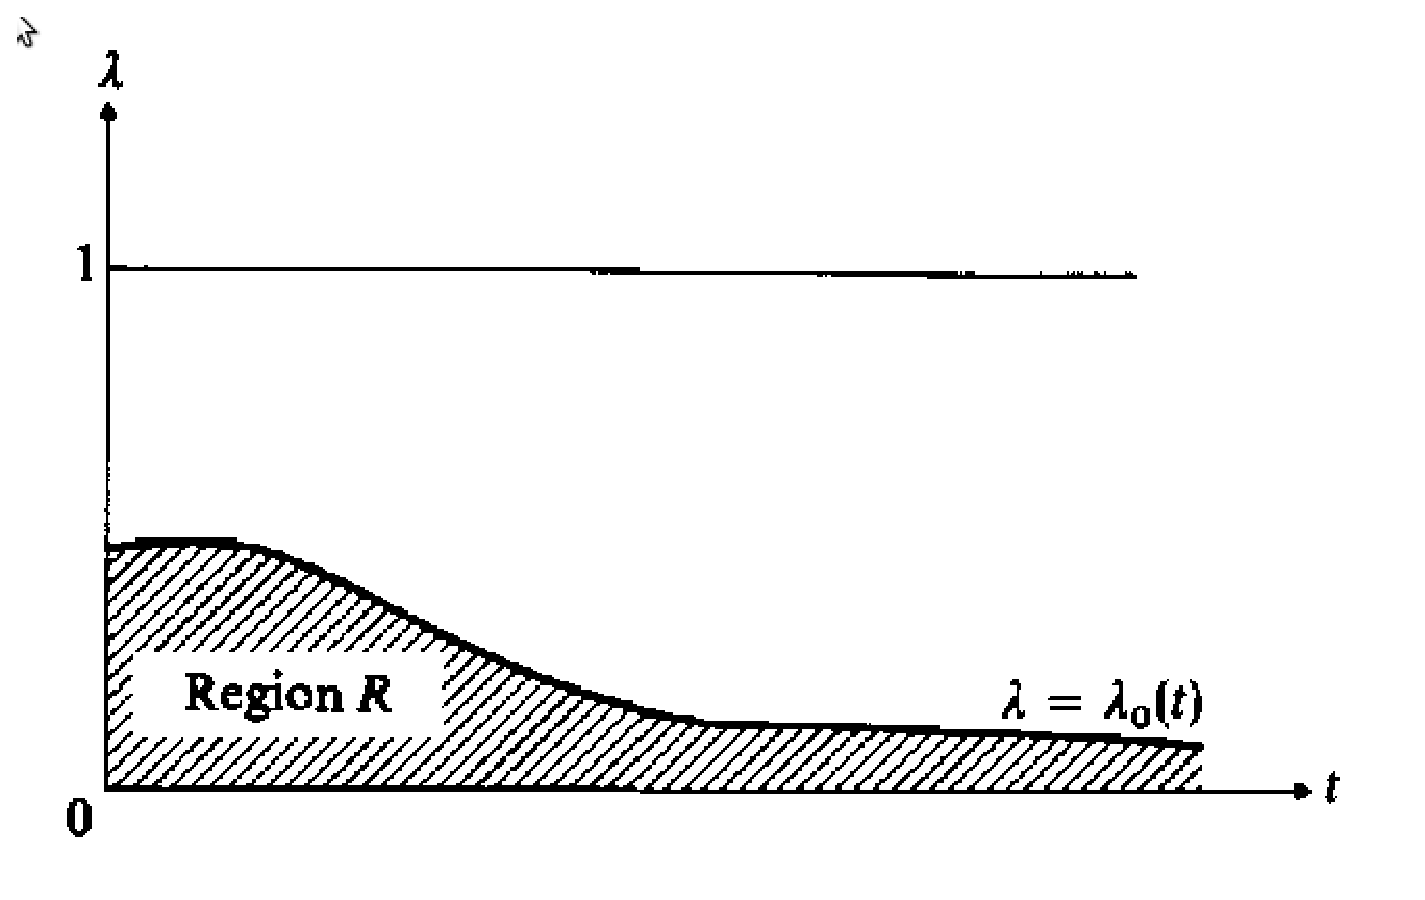
\includegraphics[scale = 0.5]{pictures/critical_region_R.eps}
\caption{Kritický region $R$ vymezený  $\lambda = \lambda_0(t)$ a $\lambda = 0$}
\label{critical-region-R}
\end{figure}
Proto můžeme testovat hypotézu na základě $\Lambda$ podmíněného $T$ - nejprve určíme hodnotu $T$ a následně provede test s pomocí intervalu $0 < \lambda < \lambda_0(t)$ s využitím pravděpodobnosti $\Lambda$ podmíněné $T$. Kritický region tak bude mít podobu plochy namísto intervalu $0 < \lambda < \lambda_0$. Tento region je navíc zkonstruován tak, že bez ohledu na skutečnou hodnotu $\theta$, má chyba typu I stále pravděpodobnost realizace $\alpha$. Připomeňme, že abychom byli schopni aplikovat tento postup, musí existovat dostatečná statistika pro $\theta$.

S využitím výše uvedeného obecného věrohodnostního poměru
\begin{equation*}
\lambda = \frac{\left(\prod_i n_{i \cdot}^{n_{i \cdot}}\right)\left(\prod_j n_{\cdot j}^{n_{\cdot j}}\right)}{n^n \prod_{i,j}n_{ij}^{n_{ij}}}
\end{equation*}
a podmíněných pravděpodobností (9.7) určit interval $0 < \lambda < \lambda_0(n_{i \cdot}; n_{\cdot j})$, který má požadovanou pravděpodobnost chyby typu I pro dané marginální součty. Při aplikaci tohoto testu však narazíme na velmi pracné odvození pravděpodobnostního rozdělení $\Lambda$ pokud $r$, $s$ a marginální součty nejsou relativně malé. Pro dostatečně velké náhodné výběry však lze použít aproximaci s vyjímkou případů, kdy $r$ a $s$ jsou rovny 2, kdy je možné použít specifickou alternativní aproximaci. Tato problematika však přesahuje záběr knihy.

Další test nulové hypotézy $\mathscr{H}_0: p_{ij} = p_{i \cdot} p_{\cdot j}; \sum p_{i \cdot} = 1, \sum p_{\cdot j} = 1$ lze odvodit nahrazením pravděpodobnostního rozdělení v (9.7) vícerozměrnou normální aproximací, kdy lze dokázat, že statistika
\begin{equation*}
Q = \sum_{i,j}\frac{[N_{ij} - n(N_{i \cdot}/n)(N_{\cdot j}/n)]^2}{n(N_{i \cdot}/n)(N_{\cdot j}/n)}
\end{equation*}
přibližně sleduje chi-kvadrát rozdělení s $rs - 1 - (r - 1 + s - 1) = (r - 1)(s - 1)$ stupni volnosti. Test zamítne $\mathscr{H}_0$ pro velká $Q$. Toto kritérium bylo poprvé navrženo Karlem Pearsonem a od $-2 \ln(\lambda)$ se liší členem řádu $1/\sqrt{n}$. Oba testy jsou tak pro dostatečně velké náhodné výběry v podstatě totožné. Statiska $Q$ má intuitivní základ. $N_{ij}$ představuje počet pozorování v $ij$-té buňce dvourozměrné kontingenční tabulky a $n(N_{i \cdot}/n)(N_{\cdot j}/n)$ představuje očekávaný počet pozorování v $ij$-té buňce za předpokladu pravdivosti $\mathscr{H}_0$. Proto dosahuje statistika $Q$ nízkých hodnot pro pravdivé $\mathscr{H}_0$ a vysokých hodnot pro nepravdivé $\mathscr{H}_0$.

\subsubsection{Třírozměrné kontingenční tabulky}

Jestliže lze každý prvek náhodného výběru klasifikovat podle tří kritérií, řekněme $A, B$ a $C$, jsme schopni tyto prvky uspořádat do tzv. třírozměrné kontingenční tabulky. Jestliže kritérium $A$ nabývá hodnot $A_i, i = 1, ..., s_1$, kritérium $B$ hodnot $B_j, j = 1, ..., s_2$ a kritérium $C$ hodnot $C_k, k = 1, ..., s_3$ pak lze tuto kontigenční tabulku chápat jako kvádr, který se skládá z $s_1 \times s_2 \times s_3$ buněk. Pravděpodobnost, že prvek náhodného výběru připadne $ijk$-té buňce označme jako $p_{ijk}$ a počet prvků v této buňce pak jako $N_{ijk}$. Marginální součty budeme, stejně jako v případě dvourozměrné kontingenční tabulky, značit tak, že příslušný index nahradíme znakem $(\cdot)$, tj.
\begin{equation*}
N_{i \cdot k} = \sum_{j = 1}^{s_2}N_{ijk} ~ \textit{a} ~ N_{\cdot \cdot k} = \sum_{i = 1}^{s_1} \sum_{j = 1}^{s_2}N_{ijk}
\end{equation*}
V souvislosti s třírozměrnou kontingenční tabulkou lze testovat čtyři hypotézy. První hypotézou je, že jsou všechna tři kritéria vzájemně nezávislá, tj.
\begin{equation}
\mathscr{H}_0: p_{ijk} = p_{i \cdot \cdot} p_{\cdot j \cdot}  p_{\cdot \cdot k}
\end{equation}
nebo lze testovat zda-li jedno ze tří kritérií je nezávislé na zbývajících dvou kritériích. Např. hypotéza, která testuje nezávislost $B$ na $A$ a $C$, má tvar
\begin{equation}
\mathscr{H}_0: p_{ijk} = p_{i \cdot k} p_{\cdot j \cdot}
\end{equation}
Postup testování těchto hypotéz je analogický postupům v případě dvourozměrných kontingečních tabulek. Věrohodnostní funkce náhodného výběru je
\begin{equation}
L = \prod_{i,j,k} p_{ijk}^{n_{ijk}}
\end{equation}
kde $\sum_{i,j,k} p_{ijk} = 1$ a $\sum_{i,j,k} n_{ijk} = n$. Pro $\overline{\underline{\Theta}}$ nastává maximum $L$ pro $\hat{p}_{ijk} = \frac{n_{ijk}}{n}$, a proto
\begin{equation}
\sup_{\overline{\underline{\Theta}}} L = \frac{1}{n^n}\prod_{i,j,k}n_{ijk}^{n_{ijk}}
\end{equation}
Např. pro testování hypotézy v (9.9) použijeme (9.9) jako substituci do (9.10) a maximalizujeme $L$ s ohledem na $p_{i \cdot k}$ a $p_{\cdot j \cdot}$, čímž získáme
\begin{equation*}
\hat{p}_{i \cdot k} = \frac{n_{i \cdot k}}{n} ~ \textit{a} ~ \hat{p}_{\cdot j \cdot} = \frac{n_{\cdot j \cdot}}{n}
\end{equation*}
a
\begin{equation}
\sup_{\overline{\underline{\Theta}}_0} L = \frac{1}{n^{2n}}\left(\prod_{i,k} n_{i \cdot k}^{n_{i \cdot k}}\right)\left(\prod_j n_{\cdot j \cdot}^{n_{\cdot j \cdot}}\right)
\end{equation}
Příslušný obecný věrohodnostní poměr $\lambda$ je pak dán podílem (9.11) a (9.12) a v případě náhodných výběrů velkého rozsahu je možné jej aproximovat pomocí $-2 \ln(\Theta)$, který sleduje chi-kvadrát rozdělení s $s_1s_2s_3 - 1 - [(s_1s_3 - 1) + s_2 - 1] = (s_1s_3 - 1)(s_2 - 1)$ stupni volnosti. $(s_1s_3 - 1) + (s_2 - 1)$ je dimenze parametrického prostoru $\overline{\underline{\Theta}}_0$ a $s_1s_2s_3 - 1$ je dimenze prostoru $\overline{\underline{\Theta}}$.

Pro hypotézu nezávislosti $B$ na $A$ a $C$, tj.
\begin{equation*}
\mathscr{H}_0: p_{ijk} = p_{i \cdot k} p_{\cdot j \cdot}
\end{equation*}
má odpovídající statistika $Q$ tvar
\begin{equation*}
Q = \sum_i \sum_j \sum_k \frac{[N_{ijk} - n(N_{i \cdot k}/n)(N_{\cdot j \cdot}/n)]^2}{n(N_{i \cdot k}/n)(N_{\cdot j \cdot }/n)}
\end{equation*}
Pro platné $\mathscr{H}_0$ sleduje $Q$ asymptoticky chi-kvadrát rozdělení s $s_1s_2s_3 - 1 - (s_1s_3 - 1) - (s_2 - 1) = (s_1s_3 - 1)(s_2 - 1)$ stupni volnosti. Statistika $Q$ má opět intuitivní základ, protože $N_{ijk}$ představuje počet prvků v buňce $ijk$ a $n(N_{i \cdot k}/n)(N_{\cdot j \cdot}/n)$ představuje očekávaný počet prvků v téže buňce za předpokladu pravdivosti $\mathscr{H}_0$.

\section{Testování hypotéz a intervaly spolehlivosti}

V předchozím textu jsme interval spolehlivosti jednorozměrného parametru $\theta$ použili pro konstrukci testu $\mathscr{H}_0: \theta = \theta_0$ vs. $\mathscr{H}_1: \theta \neq \theta_0$. Tento postup však lze také obrátit a z rodiny testů $\mathscr{H}_0: \theta = \theta_0$ vs. $\mathscr{H}_1: \theta \neq \theta_0$\footnote{Rodinu testů vytvoříme jednoduše tak, že postupně měníme $\theta_0$.} získat interval spolehlivosti pro $\theta$. Následující text je možné chápat jako úvod do problematiky.

Pojem interval spolehlivosti nahraďme obecnějším pojmem množina spolehlivosti. Stejně jako v předchozím textu označuje $\mathfrak{X}$ výběrový prostor, $\overline{\underline{\Theta}}$ parametrický prostor a $(x_1, ..., x_n)$ konkrétní realizaci náhodného výběru.

\begin{definition}[Množina spolehlivosti]
Rodina podmnožin parametrického prostoru $\overline{\underline{\Theta}}$ indexovaná skrze $(x_1, ..., x_n) \in \mathfrak{X}$, kterou označujeme jako $\vartheta =\{\underline{\overline{\Theta}}(x_1, ..., x_n): \overline{\underline{\Theta}}(x_1, ..., x_n) \subseteq \overline{\underline{\Theta}}; (x_1, ..., x_n) \in \mathfrak{X}\}$, je rodinou množin spolehlivosti s koeficietem spolehlivosti $\gamma$, jestliže pro všechna $\theta \in \overline{\underline{\Theta}}$ platí
\begin{equation*}
P_{\theta}[\overline{\underline{\Theta}}(X_1, ..., X_n) ~ \textit{obsahuje} ~ \theta] = \gamma
\end{equation*}
\end{definition}

Libovolný člen $\overline{\underline{\Theta}}(x_1, ..., x_n)$ z rodiny množin spolehlivosti je podmnožinou parametrického prostoru $\overline{\underline{\Theta}}$. $\overline{\underline{\Theta}}(X_1, ..., X_n)$ je náhodnou podmnožinou - pro konkrétní realizaci $(x_1, ..., x_n)$ náhodných veličin $(X_1, ..., X_n)$ nabývá $\overline{\underline{\Theta}}(X_1, ..., X_n)$ hodnoty $\overline{\underline{\Theta}}(x_1, ..., x_n)$, což je člen rodiny $\vartheta$. Pro dané $\theta$ je $\{\overline{\underline{\Theta}}(X_1, ..., X_n) ~ \textit{obsahuje} ~ \theta\}$ náhodným jevem. Toto $\theta$, které taktéž figuruje v $P_{\theta}$ výše uvedené věty, indexuje pravděpodobnostní rozdělení náhodných veličin $(X_1, ..., X_n)$ vystupujících v $\overline{\underline{\Theta}}(X_1, ..., X_n)$.

\begin{example}
Uvažujme náhodný výběr $X_1, ..., X_n$ z populace $N(\theta, 1)$, kde $\overline{\underline{\Theta}} = \{\theta: -\infty < \theta < \infty\}$. Nechť má podmnožina $\overline{\underline{\Theta}}(x_1, ..., x_n)$ podobu intervalu $(\overline{x} - z / \sqrt{n}, \overline{x} + z / \sqrt{n})$, kde $z$ je dáno vztahem $\Phi(z) - \Phi(-z) = \gamma$. Pak je rodina podmnožin $\vartheta = \{\overline{\underline{\Theta}}(x_1, ..., x_n): \overline{\underline{\Theta}}(x_1, ..., x_n) = (\overline{x} - z / \sqrt{n}, \overline{x} + z / \sqrt{n})\}$ rodinou množin spolehlivosti s koeficientem spolehlivosti $\gamma$, protože pro všechna $\theta \in \overline{\underline{\Theta}}$ platí
\begin{multline*}
P_{\theta}[\overline{\underline{\Theta}}(X_1, ..., X_n) ~ \textit{obsahuje} ~ \theta] = P_{\theta}\left[\overline{X} - \frac{z}{\sqrt{n}} < \theta < \overline{X} + \frac{z}{\sqrt{n}}\right]\\
= P_{\theta}\left[-z < \frac{\overline{X} - \theta}{1 / \sqrt{n}} < z \right] = \gamma
\end{multline*}
Rodina $\vartheta$ je rodinou intervalů spolehlivosti pro $\theta$ s koeficientem spolehlivosti $\gamma$.
\end{example}

Jak nyní ukážeme, lze množiny spolehlivosti zkonstruovat na základě testů hypotéz. Uvažujme nenáhodný test $\mathscr{T}_{\theta_0}$ velikosti $\alpha$ pro nulovou hypotézu $\mathscr{H}_0: \theta =  \theta_0$. Nechť $\mathfrak{X}(\theta_0)$ představuje akceptační region testu $\mathscr{T}_{\theta_0}$\footnote{Připomeňme, že akceptační region je doplňkem kritického regionu. Pro kritický region $C(\theta_0)$ tak platí $\mathfrak{X}(\theta_0) = \mathfrak{X} - C(\theta_0)$.}. Protože má test $\mathscr{T}_{\theta_0}$ má velikost $\alpha$ platí
\begin{equation*}
P_{\theta_0}[(X_1, ..., X_n) \in \mathfrak{X}(\theta_0)] = 1 - \alpha
\end{equation*}
S tím, jak měníme $\theta_0$ nad množinou $\overline{\underline{\Theta}}$, získáváme sérii testů $\mathscr{T}_{\theta_0}$ a jim odpovídající akceptačních regiony $\mathscr{X}((\theta_0): \theta_0 \in \overline{\underline{\Theta}}$. Lze definovat
\begin{equation}
\overline{\underline{\Theta}}(x_1, ..., x_n) = \{\theta_0: (x_1, ..., x_n) \in \mathfrak{X}(\theta_0)\}
\end{equation}
Je zřejmé, že $\overline{\underline{\Theta}}(x_1, ..., x_n)$ je podmnožinou $\overline{\underline{\Theta}}$. Dále platí, že $\{\overline{\underline{\Theta}}(x_1, ...,  x_n)\}$ je rodinou množin spolehlivosti s koeficientem spolehlivosti $\gamma = 1 - \alpha$, protože $\{\overline{\underline{\Theta}}(X_1, ..., X_n) ~ \textit{obsahuje} ~ \theta_0\}$ pouze, jestliže $\{(X_1, ..., X_n) \in \mathfrak{X}(\theta_0)\}$, a proto $P_{\theta_0}[\overline{\underline{\Theta}}(X_1, ..., X_n) ~ \textit{obsahuje} ~ \theta_0] = P_{\theta_0}[(X_1, ..., X_n) \in \mathfrak{X}(\theta_0)] = 1 - \alpha$.

\begin{example}
Uvažujme náhodný výběr $X_1, ..., X_n$ z populace $N(\theta, 1)$ a testujme $\mathscr{H_0}: \theta = \theta_0$. Test velikosti $\alpha$ zamítne $\mathscr{H}_0$, jestliže $|\overline{x} - \theta_0| \ge z / \sqrt{n}$, kde $z$ je dáno vztahem $\Phi(z) - \Phi(-z) = 1 - \alpha$. Akceptační region je dán
\begin{equation*}
\mathfrak{X}(\theta_0) = \left((x_1, ..., x_n): \theta_0 - \frac{z}{\sqrt{n}} < \overline{x} < \theta_0 + \frac{z}{\sqrt{n}} \right)
\end{equation*}
Dále, stejně jako v případě (9.13) definujme
\begin{multline*}
\overline{\underline{\Theta}}(x_1, ..., x_n) = \{\theta_0: (x_1, ..., x_n) \in \mathfrak{X}(\theta_0)\}\\
= \left(\theta_0: \theta_0 - \frac{z}{\sqrt{n}} < \overline{x} < \theta_0 + \frac{z}{\sqrt{n}}\right)\\
= \left(\theta_0: \overline{x} - \frac{z}{\sqrt{n}} < \theta_0 < \overline{x} + \frac{z}{\sqrt{n}}\right)
\end{multline*}
$\overline{\underline{\Theta}}(x_1, ..., x_n)$ je interval spolehlivosti s koeficientem spolehlivosti $\gamma = 1 - \alpha$.
\end{example}

Výše uvedený obecný postup ukazuje, jak lze testování hypotéz použít při konstrukci množin spolehlivosti. Tento postup však lze také obrátit a z rodiny množin spolehlivosti získat test hypotézy. Pro rodinu množin spolehlivosti $\{\overline{\underline{\Theta}}(x_1, ..., x_n)\}$ s koeficientem spolehlivosti $\gamma$ jsme definovali
\begin{equation*}
\mathfrak{X}(\theta_0) = \{(x_1, ..., x_n): \theta_0 \in \overline{\underline{\Theta}}(x_1, ..., x_n)\}
\end{equation*}
Nenáhodný test s výše uvedeným akceptačním regionem $\mathfrak{X}(\theta_0)$ je testem hypotézy $\mathscr{H}_0: \theta = \theta_0$ s velikostí $\alpha = 1 - \gamma$.

Vztah mezi testováním hypotéz a množinami spolehlivosti není užitečný pouze k tomu, že z prvního lze odvodit druhé a naopak. Další důležitou oblastí je optimalita testu resp. množiny spolehlivosti. Jestliže je daný test optimální, pak je odpovídající množina spolehlivosti taktéž optimální a naopak. Test toho tvrzení překračuje záběr této knihy, a proto se pouze omezíme na následující definici.

\begin{definition}[Uniformně nejvíce přesná rodina množin spolehlivosti]
Rodina množin spolehlivosti $\{\overline{\underline{\Theta}}^*(x_1, ..., x_n)\}$ s koeficientem spolehlivosti $\gamma$ je uniformně nejpřesnější rodinou množin spolehlivosti pro koeficient $\gamma$, jestliže pro libovolnou alternativní rodinu množin spolehlivosti $\{\overline{\underline{\Theta}}(x_1, ..., x_n)\}$ s koeficientem spolehlivosti $\gamma$ a všechna $\theta$ a $\theta'$ platí
\begin{equation*}
P_{\theta}[\overline{\underline{\Theta}}^*(X_1, ..., X_n) ~ \textit{obsahuje} ~ \theta'] \le P_{\theta}[\overline{\underline{\Theta}}(X_1, ..., X_n) ~ \textit{obsahuje} ~ \theta']
\end{equation*}
\end{definition}

Výše uvedená definice říká, že $\overline{\underline{\Theta}}^*(X_1, ..., X_n)$ obsahuje nesprávné $\theta'$ s menší pravděpodobností než $\overline{\underline{\Theta}}(X_1, ..., X_n)$, přičemž $\overline{\underline{\Theta}}^*(X_1, ..., X_n)$ a $\overline{\underline{\Theta}}(X_1, ..., X_n)$ obsahují správné $\theta$ se stejnou pravděpodobností. Problémem je, že obecné uniformně nejpřesnější množina spolehlivosti zpravidla neexistuje. Nicméně ji lze definovat nad omezeným souborem množin spolehlivosti, kde jsou šance na její existenci větší. K tomuto účelu lze opět využít vztahu mezi testem hypotéz a množinami spolehlivosti. Jestliže je $\mathscr{T}^*$ uniformně nejsilnějším testem velikosti $\alpha$ nad omezeným souborem testů pro hypotézu $\mathscr{H_0}: \theta = \theta_0$, pak je pro tento omezený soubor odpovídající množina spolehlivosti uniformně nejpřesnější s koeficientem $\gamma = 1 - \alpha$. Tímto způsobem lze přetransformovat uniformně nejsilnější test v uniformně nejpřesnější množinu spolehlivosti.

\section{Sekvenční testování hypotéz}

\subsection{Úvod}

Sekvenční testování hypotéz je charakteristické tím, že se velikost náhodného výběru odvíjí od průběhu testu a namísto toho, aby byla dána před samotným testováním. V následujícím textu se zaměříme na jednu z forem sekvenčního testování hypotéz a to na sekvenční pravděpodobnostní poměr.

Uvažujme test ve formě $\mathscr{H}_0: \theta = \theta_0$ vs. $\mathscr{H}_1: \theta = \theta_1$. Dle Neyman-Pearsonovy věty platí, že v případě náhodného výběru velikosti $n$ a chyby typu II velikosti $\alpha$ lze velikost $\beta$ chyby typu I minimalizovat pomocí testu založeného na věrohodnostím poměru. To znamená, že pro dané $\alpha$ a $n$ minimalizujeme $\beta$. Nyní předpokládejme, že pro dané $\alpha$ i $\beta$ chceme stanovit velikost náhodného výběru $n$, pro kterou má odpovídající věrohodnostní poměr chybu I resp. II typu o velikosti $\alpha$ resp. $\beta$. Řešení takovéhoto problému ilustruje následující příklad

\begin{example}
Výrobce ví, že doba živostnosti jeho výrobku je dána $N(100, 100)$. Aby přijal nový výrobní proces, chce si být jistý, že tento proces povede k navýšení střední doby životnosti alespoň o 5\%. K tomuto účelu podrobí testu výrobky z zkušebního provozu, které jsou vyrobeny novým postupem.

Předpokládejme, že doba životnosti výrobku ze zkušebního provozu je $N(\theta, 100)$ a že testujeme $\mathscr{H}_0: \theta \le 100$ vs. $\mathscr{H}_1: \theta > 100$. Zafixujme velikosti chyby typu I a II na 1\% a 5\% a pokusme se nalézt velikost zkušebního vzorku. Platí
\begin{equation*}
0.01 = P_{\theta = 100}[\overline{X}_n > k] ~ \textit{a} ~ 0.05 = P_{\theta = 105}[\overline{X} \le k]
\end{equation*}
neboli
\begin{equation*}
0.01 = 1 - \Phi \left(\frac{k - 100}{10 / \sqrt{n}}\right) ~ \textit{a} ~ 0.05 = \Phi \left(\frac{k - 105}{10 / \sqrt{n}}\right)
\end{equation*}
První z rovnic lze převést do tvaru $\Phi \left(\frac{k - 100}{10 / \sqrt{n}}\right) = 0.99$, což implikuje
\begin{equation*}
\frac{k - 100}{10 / \sqrt{n}} \approx 2.326
\end{equation*}
Druhá rovnice $\Phi \left(\frac{k - 105}{10 / \sqrt{n}}\right) = 0.05$ pak implikuje
\begin{equation*}
\frac{k - 105}{10 / \sqrt{n}} \approx -1.645
\end{equation*}
Jestliže z obou vztahů vyjádříme $k$ a dáme je do rovnosti, získáme
\begin{equation*}
100 + 10 \cdot 2.326 / \sqrt{n} \approx 105 - 10 \cdot 1.645 / \sqrt{n}
\end{equation*}
Řešením je pak $n \approx 63.08$, tj. potřebujeme vzorek o velikosti 64 výrobků.
\end{example}

Ve výše uvedeném případě nemusí být vždy nutné otestovat všech 64 výrobků, abychom byli schopni přijmout či zamítnout nulovou hypotézu. Může se totiž stát, že již během prvních 20, 30 či 40 pozorování získáme dostatečné důkazy k tomu, abychom pro dané $\alpha$ a $\beta$ nulovou hypotézy přijali popř. zamítli. To znamená, že je zde možnost zkonstruovat takový test, který by v průměru umožnil ukončit testování před dosažením počtu 64 pozorování. Tímto se dostáváme k následující kapitole.

\subsection{Definice sekvenčního poměrového testu}

Uvažujme dvě populace a náhodný výběr, o kterém nevíme, ze které populace pochází. Předpokládejme, že naším cílem je tento náhodný výběr přiřadit jedné z populací. Testujeme tedy $\mathscr{H}_0: X_i ~ f_0(\cdot)$ vs. $\mathscr{H}_1: X_i ~ f_1(\cdot)$. Připomeňme, že věrohodnostní poměrový test zamítl $\mathscr{H}_0$, jestliže
\begin{equation*}
\lambda = \frac{L_0}{L_1} \le k
\end{equation*}
pro určitou konstantu $k > 0$. Sekvenční poměrový test je založen na sérii takovýchto testů. Definujme
\begin{equation*}
\lambda_m = \lambda_m(x_1, ..., x_m) = \frac{L_0(x_1, ..., x_m)}{L_1(x_1, ..., x_m)} = \frac{L_0(m)}{L_1(m)} = \frac{\prod_{i = 1}^m f_0(x_i)}{\prod_{i = 1}^m f_1(x_i)}
\end{equation*}
pro $m = 1, 2 , ...$ a postupně vypočtěme $\lambda_1, \lambda_2, ...$. Pro fixní $k_0$ a $k_1$, které splňují podmínku $0 < k_0 < k_1$, aplikujme následující postup.
\begin{enumerate}
\item Realizujeme pozorování $x_1$ a vypočteme pro něj poměr $\lambda_1$.
\item Jestliže $\lambda_1 \le k_0$, zamítneme $\mathscr{H}_0$ a ukončíme testování.
\item Jestliže $\lambda_1 \ge k_1$, přijmeme $\mathscr{H}_0$ a ukončíme testování.
\item Jestliže $k_0 < \lambda_1 < k_1$, realizujeme pozorování $x_2$ a vypočteme $\lambda_2$.
\item Jestliže $\lambda_2 \le k_0$, zamítneme $\mathscr{H}_0$ a ukončíme testování.
\item Jestliže $\lambda_2 \ge k_1$, přijmeme $\mathscr{H}_0$ a ukončíme testování.
\item Jestliže $k_0 < \lambda_2 < k_1$, realizujeme pozorování $x_3$ a vypočteme $\lambda_3$.
\item Postupně navyšujeme počet pozorování a aplikujeme výše popsaný postup, dokud
\begin{enumerate}
\item $\lambda_i \le k_0$, kdy zamítneme $\mathscr{H}_0$ a ukončíme testování
\item $\lambda_i \ge k_1$, kdy přijmeme $\mathscr{H}_0$ a ukončíme testování
\end{enumerate}
\end{enumerate}
Kritický region výše popsaného sekvenčního testu je $C = \cup_{n = 1}^{\infty}C_n$, kde
\begin{equation*}
C_n = \{(x_1, ..., x_n): k_0 < \lambda_j(x_1, ..., x_j) < k_1, j = 1, ..., n -1, \lambda_n(x_1, ..., x_n) \le k_0\}
\end{equation*}
Podobně akceptační region je $A = \cup_{n = 1}^{\infty} A_n$, kde
\begin{equation*}
A_n = \{(x_1, ..., x_n): k_0 < \lambda_j(x_1, ..., x_j) < k_1, j = 1, ..., n - 1, \lambda_n(x_1, ..., x_n) \ge k_1\}
\end{equation*}

\begin{definition}[Sekvenční poměrový test]
Pro dané $0 < k_0 < k_1$ je výše popsaný test označován jako sekvenční poměrový test.
\end{definition}

V předchozím textu jsme se pro dané $n$ snažili stanovit $k$ tak, aby výsledný test měl velikost $\alpha$. Nyní se pokusíme stanovit $k_0$ a $k_1$ takové, aby výsledný sekvenční poměrový test měl chyby typu I resp. II předem dané velikosti $\alpha$ resp. $\beta$. Všimněme si, že
\begin{equation*}
\alpha = P[\textit{zamítnutí} ~ \mathscr{H}_0 | \mathscr{H}_0 je pravdivé] = \sum_{n = 1}^{\infty} \int_{C_n} L_0(n)
\end{equation*}
a
\begin{equation*}
\beta = P[\textit{přijetí} ~ \mathscr{H}_0 | \mathscr{H}_0 je nepravdivé] = \sum_{n = 1}^{\infty} \int_{A_n} L_1(n)
\end{equation*}
kde, stejně jako dříve, představuje $\int_{C_n} L_0(n)$ zkrácený zápis pro $\int \cdots \int_{C_n}\left(\prod_{i = 1}^n f_0(x_i)dx_i\right)$. Protože $A_n$ a $C_n$ jsou vyjádřeny ve formě $k_0$ a $k_1$, lze pro fixní $\alpha$ a $\beta$ výše uvedené dvě rovnice chápat jako rovnice o dvou neznámých $k_0$ a $k_1$. Jejich řešením pak získáme sekvenční poměrový test s chybami o velikosti $\alpha$ a $\beta$. Jak je však při pohledu na tyto dvě rovnice patrné, je výpočet $k_0$ a $k_1$ poměrně komplikovanou záležitostí. Naštěstí však existuje poměrně jednoduchá aproximace, kterou si představíme následující kapitole.

V rámci sekvečního poměrového testu navyšujeme počet pozorování, dokud se $\lambda_n(x_1, ..., x_n)$ nenachází mimo interval $(k_0, k_1)$. Velikost náhodného vzorku v rámci testu tak závisí na realizacích $x_1, x_2, ...$ náhodných veličin $X_1, X_2, ...$, a proto se jedná taktéž o náhodnou veličinu. Označme ji písmenem $N$. Jedním ze způsobů hodnocení sekvenčních poměrových testů je porovnání střední hodnoty $N$, kde preferujeme test s nižší střední hodnotou. Tímto se dostáváme k následující větě, kterou uvádíme bez důkazu.

\begin{theorem}
Sekvenční poměrový test, který splňuje
\begin{equation*}
P[\mathscr{H}_0 ~ \textit{je zamítnuto}| \mathscr{H_0} ~ \textit{je pravdivé}] \le \alpha
\end{equation*}
a
\begin{equation*}
P[\mathscr{H}_0 ~ \textit{je přijmuto}| \mathscr{H_0} ~ \textit{je nepravdivé}] \le \beta
\end{equation*}
minimalizuje v porovnání se všemi alternativními testy s chybami velikosti $\alpha$ a $\beta$ jak
\begin{equation*}
E[N|\mathscr{H}_0 ~ \textit{je pravdivé}]
\end{equation*}
tak
\begin{equation*}
E[N|\mathscr{H}_0 ~ \textit{je nepravdivé}]
\end{equation*}
V tomto směru je tedy tento sekvenční poměrový test optimální.
\end{theorem}

\subsection{Přibližný sekvenční poměrový test}

V předchozím textu jsme konstatovali, že výpočet parametrů $k_0$ a $k_1$, které jsou nezbytné pro definování sekvenčního poměrového testu, je poměrně komplikovaný. Naštěstí existuje relativně jednoduchá aproximace těchto parametrů.

\begin{corollary}
Nechť jsou $k_0$ a $k_1$ definovány tak, že jim odpovídající sekvenční poměrový test má chyby velikosti $\alpha$ a $\beta$. Parametry $k_0$ a $k_1$ lze aproximovat pomocí
\begin{equation*}
k_0' = \frac{\alpha}{1 - \beta} ~~~ \textit{a} ~~~ k_1' = \frac{1 - \alpha}{\beta}
\end{equation*}
\end{corollary}

\begin{proof}
Předpokládejme, že $\sum_{n = 1}^{\infty} P[N = n|\mathscr{H}_i] = 1$ pro $i = 0, 1$. Z definice chyby typu I a poměrového testu vyplývá
\begin{multline*}
\alpha = P[\textit{zamítnutí} ~ \mathscr{H}_0 | \mathscr{H}_0 ~ \textit{je pravdivé}] = \sum_{n = 1}^{\infty} \int_{C_n}L_0(n) \le \sum_{n = 1}^{\infty} \int_{C_n} k_0 L_1(n)\\
= k_0 \sum_{n = 1}^{\infty} \int_{c_n} L_1(n) = k_0 P[\textit{zamítnutí} ~ \mathscr{H}_0 | \mathscr{H}_1 ~ \textit{je pravdivé}] = k_0 (1 - \beta)
\end{multline*}
a proto $k_0 \ge \frac{\alpha}{1 - \beta}$. Zároveň však také platí
\begin{multline*}
1 - \alpha = P[\textit{přijetí} ~ \mathscr{H}_0 | \mathscr{H}_0 ~ \textit{je pravdivé}] = \sum_{n = 1}^{\infty} \int_{A_n} L_0(n) \ge \sum_{n = 1}^{\infty} \int_{A_n} k_1 L_1(n)\\
= k_1 P[\textit{přijetí} ~ \mathscr{H}_0 | \mathscr{H}_1 ~ \textit{je pravdivé}] = k_1 \beta
\end{multline*}
a proto $k_1 \le \frac{1 - \alpha}{\beta}$. Všimněme si, že aproximace $k_0' = \frac{\alpha}{1 - \beta}$ a $k_1' = \frac{1 - \alpha}{\beta}$ splňují
\begin{equation*}
k_0' = \frac{\alpha}{1 - \beta} \le k_0 < k_1 \le \frac{1 - \alpha}{\beta} = k_1'
\end{equation*}
\end{proof}

\begin{corollary}
Jestliže jsou $\alpha'$ a $\beta'$ velikosti chyb sekvenčního poměrového testu definovaného pomocí $k_0'$ a $k_1'$, pak platí $\alpha' + \beta' \le \alpha + \beta$.
\end{corollary}

\begin{proof}
Nechť $A'$ resp. $C'$ označuje akceptační resp. kritický region sekvenčního poměrového testu definovaného pomocí $k_0'$ a $k_1'$. Pak platí
\begin{equation*}
\alpha' = \sum_{n = 1}^{\infty} \int_{C_n'} L_0(n) \le \frac{\alpha}{1 - \beta} \sum_{n = 1}^{\infty} \int_{C_n'}L_1(n) = \frac{\alpha}{1 - \beta}{1 - \beta'}
\end{equation*}
a
\begin{equation*}
1 - \alpha' = \sum_{n = 1}^{\infty} \int_{A_n'} L_0(n) \ge \frac{1 - \alpha}{\beta} \sum_{n = 1}^{\infty}\int_{A_n'}L_1(n) = \frac{1 - \alpha}{\beta} \beta'
\end{equation*}
a proto $\alpha'(1 - \beta) \le \alpha(1 - \beta')$ a $(1 - \alpha)\beta' \le (1 - \alpha')\beta$, což v souhrnu implikuje $\alpha'(1 - \beta) + (1 - \alpha)\beta' \le \alpha(1 - \beta') + (1 - \alpha')\beta$ neboli $\alpha' + \beta' \le \alpha + \beta$.
\end{proof}

Ideálně bychom preferovali sekvenční poměrový test, který má chyby o předem daných velikostech $\alpha$ a $\beta$. Protože je však složité nalézt odpovídající $k_0$ a $k_1$, použijeme testt definovaný pomocí jejich aproximací $k_0'$ a $k_1'$ s vědomím, že součet chyb $\alpha'$ a $\beta'$ je menší nebo roven součtu požadovaných chyb $\alpha$ a $\beta$.

\subsection{Přibližná střední hodnota velikosti náhodného výběru sekvenčního poměrového testu}

Sekvenční poměrový test probíhá tak dlouho, dokud $k_0 < \lambda_m < k_1$ a skonční jakmile $\lambda_m \le k_0$ nebo $\lambda_m \ge k_1$. Definujme $z_i = \ln \left(\frac{f_0(x_i)}{f_1(x_i)}\right)$. V rámci ekvivalentního testu pak navyšujeme velikost vzorku dokud $\ln(k_0) < \sum_{i = 1}^m z_i < \ln(k_1)$ a test ukončíme, jestliže $\sum_{i = 1}^m z_i \le \ln(k_0)$, kdy $\mathscr{H}_0$ zamítneme, nebo $\sum_{i = 1}^m z_i \ge \ln(k_1)$, kdy $\mathscr{H}_0$ přijmeme. Stejně jako v předchozím textu i zde představuje náhodná veličina $N$ velikost vzorku sekvenčního poměrového testování. Dále definujme $Z_i = \ln\left(\frac{f_0(X_i)}{f_1(X_i)}\right)$. Následující věta slouží k určení přibližné střední hodnoty velikosti výběru pro sekvenční poměrový test.

\begin{theorem}[Waldova rovnice]
Uvažujme nezávislé náhodné veličiny $Z_1, ..., Z_n, ...$ s identickým pravděpodobnostním rozdělením. Nechť tyto náhodné veličiny splňují podmínku $E[|Z_i| < \infty]$ a nechť $N$ je náhodná veličina, která nabývá hodnot z oboru přirozených čísel. Pak platí
\begin{equation*}
E[Z_1 + ... + Z_n] = E[N] \cdot E[Z_i]
\end{equation*}
\end{theorem}

\begin{proof}
\begin{multline*}
E[Z_1 + ... + Z_N] = E[E[Z_1 + ... + Z_N] | N]\\
= \sum_{n = 1}^{\infty} E[Z_1 + ... + Z_n| N = n] P[N = n] = \sum_{n = 1}^{\infty} \sum_{i = 1}^n E[Z_i|N = n]P[N = n]\\
= \sum_{i = 1}^{\infty} \sum_{n = 1}^{\infty} E[Z_i|N = n]P[N = n] = \sum_{i = 1}^{\infty} E[Z_i|N \ge i]P[N \ge i]\\
= \sum_{i = 1}^{\infty}E[Z_i]P[N \ge i] = E[Z_i]\sum_{i = 1}^{\infty}P[N \ge i] = E[Z_i] E[N]
\end{multline*}
Při úpravách jsme použili vztah $E[Z_i] = E[Z_i|N \ge i]$. Tento vztah platí, protože $\{N \ge i\}$ závisí pouze na $Z_1, ..., Z_{i - 1}$, a proto je nezávislý na $Z_i$. Vztah $E[N] = \sum_{i = 1}^{\infty}P[N \ge i]$ pak vychází z bodu (3) definice střední hodnoty (2.11).
\end{proof}

Jestliže sekvenční pravděpodobnostní test vede k zamítnutí $\mathscr{H}_0$, pak $Z_1 + ... + Z_N \le \ln(k_0)$, nicméně $Z_1 + ... + Z_N$ je relativně blízké $\ln(k_0)$, protože $Z_1 + ... + Z_N$ se stane poprvé menší nebo rovno $\ln(k_0)$ pro $N$-té pozorování. Proto platí $E[Z_1 + ... + Z_N] \approx \ln(k_0)$. Podobně, jestliže test vede k přijetí $\mathscr{H}_0$, platí $E[Z_1 + ... + Z_n] \approx \ln(k_1)$. Proto $E[Z_1 + ... + Z_N] \approx \rho \ln(k_0) + (1 - \rho)\ln(k_1)$, kde $\rho = P[\mathscr{H}_0 ~ \textit{je zamítnuto}]$. S využitím
\begin{equation*}
E[N] = \frac{E[Z_1 + ... + Z_N]}{E[Z_1]} \approx \frac{\rho \ln(k_0) + (1 - \rho)\ln(k_1)}{E[Z_i]}
\end{equation*}
získáme
\begin{multline}
E[N | \mathscr{H}_0 ~ \textit{je pravdivé}] \approx \frac{\alpha \ln(k_0) + (1 - \alpha)\ln(k_1)}{E[Z_i|\mathscr{H}_0 ~ \textit{je pravdivé}]}\\
\approx \frac{\alpha \ln[\alpha / (1 - \beta)] + (1 - \alpha)\ln[(1 - \alpha) / \beta]}{E[Z_i | \mathscr{H}_0 ~ \textit{je pravdivé}]}
\end{multline}
a
\begin{multline}
E[N | \mathscr{H}_0 ~ \textit{je nepravdivé}] \approx \frac{(1 - \beta) \ln(k_0) + \beta \ln(k_1)}{E[Z_i|\mathscr{H}_0 ~ \textit{je nepravdivé}]}\\
\approx \frac{(1 - \beta) \ln[\alpha / (1 - \beta)] + \beta \ln[(1 - \alpha) / \beta]}{E[Z_i | \mathscr{H}_0 ~ \textit{je nepravdivé}]}
\end{multline}

\begin{example}
Uvažujme náhodný výběr z $N(\theta, \sigma^2)$, kde $\sigma^2$ známe. Testujme $\mathscr{H}_0> \theta = \theta_0$ vs. $\mathscr{H}_1: \theta = \theta_1$. Platí
\begin{multline*}
z_i = \ln \left(\frac{f_0(x_i)}{f_1(x_i)}\right) = \ln \left(\frac{(1 / \sqrt{2 \pi} \sigma)e^{-\frac{1}{2}[(x_i - \theta_0)/\sigma]^2}}{(1 / \sqrt{2 \pi} \sigma)e^{-\frac{1}{2}[(x_i - \theta_0)/\sigma]^2}}\right)\\
= - \frac{1}{2 \sigma^2}[(x_i - \theta_0)^2 - (x_i - \theta_1)^2] = -\frac{1}{2 \sigma^2}[(\theta_0^2 - \theta_1^2) - 2x_i(\theta_0 - \theta_1)]
\end{multline*}
a proto
\begin{equation*}
E[Z_i | \mathscr{H}_0 ~ \textit{je pravdivé}] = -\frac{1}{2 \sigma^2}[(\theta_0^2 - \theta_1^2) - 2 \theta_0(\theta_0 - \theta_1)] = \frac{1}{2 \sigma^2}(\sigma_1 - \sigma_0)^2
\end{equation*}
a
\begin{equation*}
E[Z_i | \mathscr{H}_0 ~ \textit{je nepravdivé}] = - \frac{1}{2 \sigma^2}(\theta_1 - \theta_0)^2
\end{equation*}
Vraťme se k příkladu (9.27). Dle zadání tohoto příkladu je $\alpha = 0.01, \beta = 0,05, \sigma^2 = 100, \theta_0 = 100$ a $\theta_1 = 105$. Dosazením do (9.14) a (9.15) získáváme
\begin{equation*}
E[N|\mathscr{H}_0 ~ \textit{je pravdivé}] \approx \frac{0.01 \ln(0.01 / 0.95) + 0.99 \ln(0.99 / 0.05)}{25 / 200} \approx 24
\end{equation*}
a
\begin{equation*}
E[N | \mathscr{H}_0 ~ \textit{je nepravdivé}] \approx 34
\end{equation*}
Pro sekvenční poměrový test jsou tedy průměrné velikosti vzorku 24 resp. 34 výrobků. Pro test s pevně danou velikostí vzorku jsem v příkladě (9.27) dospěli k počtu 64 produktů. 
\end{example}

\chapter{Lineární regrese}

\section{Příklady lineární regrese}

\begin{example}
Vzdálenost $s$, kterou částice urazí v čase $t$ je dána rovnicí $s = \beta_0 + \beta_1t$, kde $\beta_1$ je průměrnou rychlostí a $\beta_0$ je pozice v čase $t = 0$. Jestliže $\beta_0$ a $\beta_1$ neznáme, pak lze pozorovat $s$ pro dvě rozdílná $t$ a z odpovídajících dvou rovnic vyřešit $\beta_0$ a $\beta_1$. Pokud např. $s = 2$ pro $t = 1$ a $s = 11$ pro $t = 4$, získáme rovnice $2 = \beta_0 + \beta_1$ a $11 = \beta_0 + 4 \beta_1$, jejichž řešením je $\beta_0 = -1$ a $\beta_1 = 3$, tj. $s = -1 + 3t$.

Předpokládejme, že měření vzdálenosti je zatíženou náhodnou chybou. Proto namísto $s$ pozorujeme $Y = s + E$, kde $E$ představuje chybu s nulovou střední hodnotou. Substitucí za $s$ tak získáme
\begin{equation*}
Y = \beta_0 + \beta_1t + E
\end{equation*}
kde $Y$ je náhodná veličina, jejíž realizaci jsme schopni pozorovat, a $E$ je náhodná veličina, jejíž realizaci schopni pozorovat nejsme. $t$ je nenáhodná veličina a $\beta_0$ a $\beta_1$ představují neznámé parametry. Hodnotu $\beta_0$ a $\beta_1$ nejsme schopni vypočíst ze dvou pozorování $(t,Y)$, jako tomu bylo v případě $(t, s)$, protože neexistuje žádná funkční závislost mezi $Y$ a $t$. Cílem našeho snažení je nalézt $\beta_0$ a $\beta_1$ a odvodit tak vztah $s = \beta_0 + \beta_1t$ pro různé hodnoty $t$. Protože $s$ je zatíženo chybami a nelze ho přímo pozorovat, nemůžeme znát ani $\beta_0$ a $\beta_1$. Nicméně na základě pozorování různých $(t,Y)$ lze s využitím statistických metod odhadnout $\beta_0$, $\beta_1$ a $s$.
\end{example}

\begin{example}
Uvažujme vztah mezi výškou jedince $h$ a jeho hmotností $w$. Je zřejmé, že neexistuje žádný funkční vztah mezi $h$ a $w$, nicméně se dá očekávat, že mezi nimi existuje určitá závislost.

Předpokládejme, že výška a váha jsou náhodné veličiny $(W,H)$, které sledují dvourozměrné normální rozdělení. Očekávaná hodnota $H$ pro danou hodnotu $w$ náhodné veličiny $W$, je dána vztahem
\begin{equation*}
E[H|W = w] = \beta_0 + \beta_1 w
\end{equation*}
kde $\beta_0$ a $\beta_1$ jsou parametry dvourozměrného normálního rozdělení. Ačkoliv mezi $H$ a $W$ neexistuje funkční vztah, existuje mezi nimi, pokud předpokládáme sdruženě normální rozdělení, lineární závislost. Proto platí
\begin{equation*}
E[H|W = w] = \beta_0 + \beta_1w
\end{equation*}
nebo také
\begin{equation*}
H_w = \beta_0 + \beta_1 w + E
\end{equation*}
kde $E$ je chyba, která sleduje normální rozdělení.
\end{example}

\section{Definice regresního modelu}

Uvažujme lineární funkci $\mu(\cdot)$ reálné proměnné $x$, tj. $\mu(x) = \beta_0 + \beta_1 x$, kde $x \in D$. Množina $D$ je obykle reprezentována celou reálnou přímkou popř. polopřímkou nebo intervalem. Předpokládejme, že existuje taková rodina kumulativních distribučních funkcí (pro každé $x$ jedna), jejichž střední hodnota pro dané $x = x_0$ je rovna $\beta_0 + \beta_1 x_0$. To znamená, že střední hodnoty těchto kumulativních distribučních funkcí tvoří přímku definovanou jako $\mu(x) = \beta_0 + \beta_1x$, jak je ilustorováno obrázkem (\ref{linear-model}).

\begin{figure}[htp]
\centering
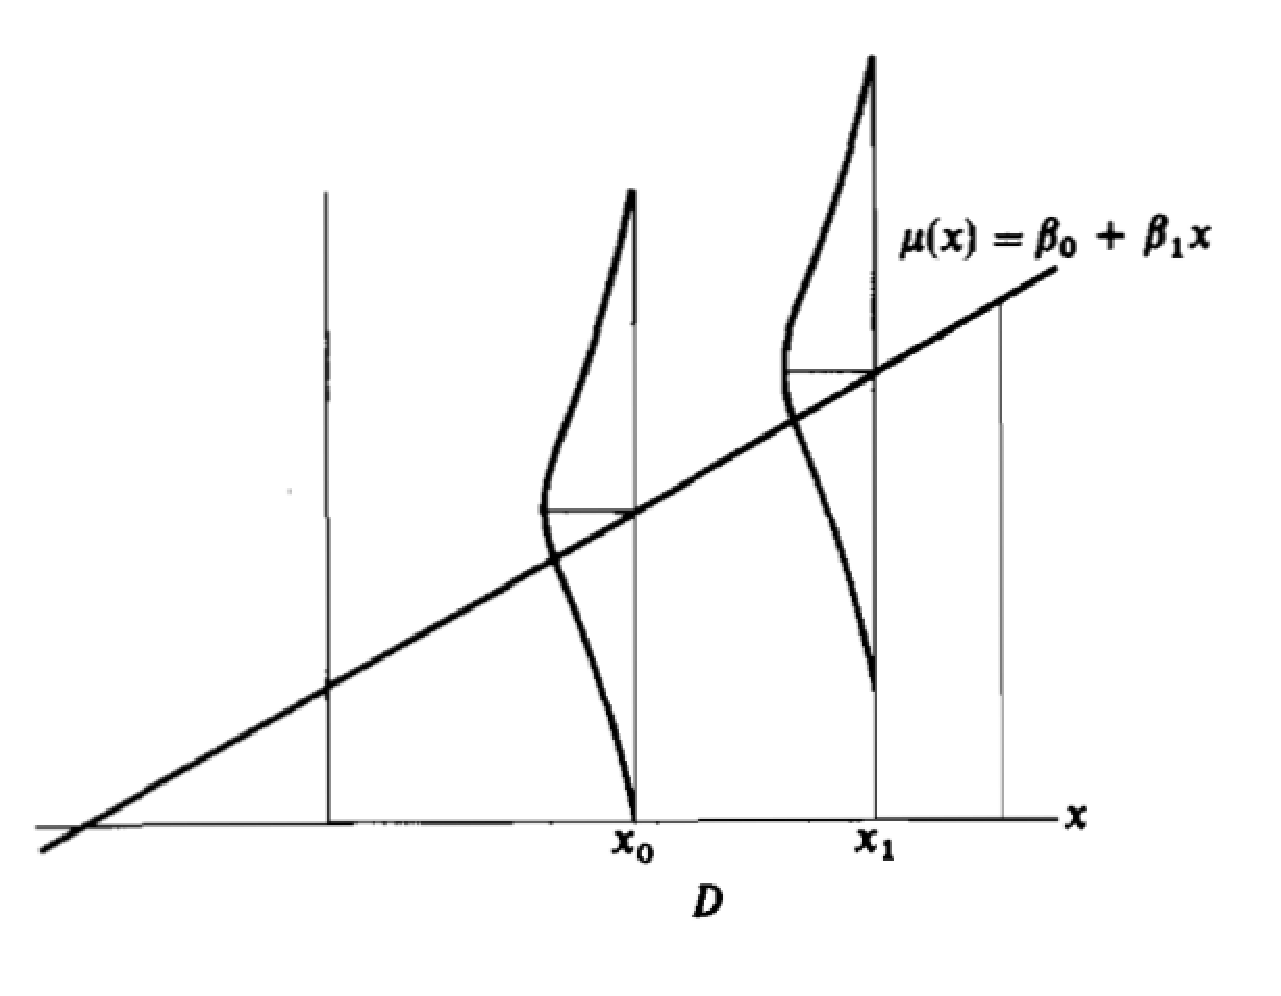
\includegraphics[scale = 0.5]{pictures/linear_model.eps}
\caption{Lineární regrese}
\label{linear-model}
\end{figure}

Cílem je na základě náhodného výběru z několika těchto kumulativních distribučních funkcí získat odhad parametrů $\beta_0$ a $\beta_1$. Toho je dosaženo následovně.
\begin{enumerate}
\item Soubor $n$ pozorování hodnot $x$ označme jako $x_1, ..., x_n$. Soubor $x_1, ..., x_n$ není souborem náhodných veličin, nicméně může být vybrán jak náhodně tak na základě vědomé selekce.
\item Každé $x_i$ určuje kumulativní distribuční funkci se střední hodnotou $\beta_0 + \beta_1 x_i$ a rozptylem $\sigma^2$. Z této kumulativní distribuční funkce je náhodně vybrána jedna hodnota označovaná jako $Y_i$. Tímto způsobem získáme $n$ uspořádaných dvojic $(Y_1, x_1), ... (Y_n, x_n)$. V předchozím textu jsme předpokládali
\begin{equation*}
E[Y_i] = \beta_0 + \beta_1 x_i ~~~ D[Y_i] = \sigma^2
\end{equation*}
Proto jsme schopni definovat náhodné veličiny $E_1, ..., E_n$ jako
\begin{equation*}
E_i = Y_i - \beta_0 - \beta_1 x_i, ~~~ i = 1, ..., n
\end{equation*}
kde $E[E_i] = 0$ a $D[E] = \sigma^2$.
\end{enumerate}
Výše uvedený vztah lze převést do tvaru
\begin{equation*}
Y_i = \beta_0 + \beta_1 x_i + E_i, ~~~ i = 1, ..., n
\end{equation*}
kde $E[E_i] = 0$ a $D[E_i] = \sigma^2$, což je definice jednoduché lineární regrese.

\begin{definition}[Lineární regrese]
Uvažujme funkci $\mu(x) = \beta_0 + \beta_1x$ pro všechna $x \in D$. Pro každé $x$ z $D$ uvažujme kumulativní distribuční funkci $F_{Y_x}(\cdot)$ se střední hodnotou $\mu(x) = \beta_0 + \beta_1 x$ a rozptylem $\sigma^2$. Nechť $x_1, ..., x_n$ představuje soubor $n$ (nikoliv nutně náhodných) pozorování z $D$. Pro $x_i$ uvažujme jednoprvkový náhodný výběr $Y_i$ z $F_{Y_{x_i}}(\cdot)$, kde $i = 1, ..., n$. Pak $(Y_1, x_1), ..., (Y_n, x_n)$ představuje soubor $n$ uspořádaných dvojic, které jsou ``provázány'' vztahem
\begin{equation*}
E[Y_i] = \beta_0 + \beta_1 x_i
\end{equation*}
a
\begin{equation*}
D[Y_i] = \sigma^2
\end{equation*}
kde $i = 1, ..., n$. Výše uvedené rovnice je možné vyjádřit také ve tvaru
\begin{gather*}
Y_i = \beta_0 + \beta_1 x_i + E_i\\
E[E_i] = 0\\
D[E_i] = \sigma^2
\end{gather*}
kde $i = 1, ..., n$.

Tyto vztahy a podmínky definují jednoduchý regresní model.
\end{definition}

Slovo ``lineární'' v pojmu ``lineární regrese'' odpovídá skutečnosti, že funkce $\mu(\cdot)$ je lineární v parametrech $\beta_0$ a $\beta_1$. Proto je $Y = \mu(x) + E$, kde $\mu(x) = \beta_0 + \beta_1 e^x$, také lineární regresí. Na kumulativní distribuční funkci $F_{Y_x}(\cdot)$ jsou zpravidla kladeny další požadavky jako např. normalita. Dále je způsob náhodného výběru takový, že $Y_i$ jsou buďto sdruženě nezávislé nebo párově nezávislé. Tímto se dostáváme k definici dvou základních případů, na které se budeme odkazovat v následujících kapitolách.

\begin{itemize}
\item \textbf{Případ A} - V tomto případě je všech $n$ náhodných veličin $Y_i$ sdruženě nezávislých a každé $Y_i$ sleduje normální rozdělení.
\item \textbf{Případ B} - V tomto případě jsou $Y_i$ párově nezávislé, tj. $cov(Y_i, Y_j) = 0$ pro všechna $i \neq j = 1, ..., n$.
\end{itemize}

Pro případ A budeme diskutovat
\begin{enumerate}
\item bodový odhad $\beta_0, \beta_1, \sigma^2$ a $\mu(x)$ pro libovolné $x \in D$
\item interval spolehlivosti pro $\beta_0, \beta_1, \sigma^2$ a $\mu(x)$ pro libovolné $x \in D$
\item testování hypotéz pro $\beta_0, \beta_1$ a $\sigma^2$
\end{enumerate}

Pro případ B budeme diskutovat
\begin{enumerate}
\item bodový odhad $\beta_0, \beta_1, \sigma^2$ a $\mu(x)$ pro libovolné $x \in D$
\end{enumerate}

\section{Bodový odhad - případ A}

V tomto případě jsou $Y_1, ..., Y_n$ nezávislé normální veličiny se středními hodnotami $\beta_0 + \beta_1 x_1, ..., \beta_0 + \beta_1 x_n$ a rozptylem $\sigma^2$. Pro účely bodového odhadu použijeme metodu maximální věrohodnosti. Věrohodnostní funkce má tvar
\begin{equation}
L(\beta_0, \beta_1, \sigma^2) = L(\beta_0, \beta_1, \sigma^2; y_1, ..., y_n)\\
= \prod_{i = 1}^n\left(\frac{1}{\sqrt{2 \pi} \sigma}e^{-\frac{1}{2}\left(\frac{y_i - \beta_0 - \beta_1x_i}{\sigma}\right)^2}\right)
\end{equation}
a
\begin{equation*}
\ln\left(L(\beta_0, \beta_1, \sigma^2)\right) = - \frac{n}{2}\ln(2 \pi) - \frac{n}{2}\ln(\sigma^2) - \frac{1}{2 \sigma^2} \sum_{i = 1}^n(y_i - \beta_0 - \beta_1 x_i)^2
\end{equation*}
V dalším kroku jsou parciální derivace $\ln\left(L(\beta_0, \beta_1, \sigma^2)\right)$ vzhledem k $\beta_0, \beta_1$ a $\sigma^2$ položeny rovno nule. Řešení těchto tří rovnic označme jako $\hat{\beta}_0, \hat{\beta}_1$ a $\tilde{\sigma}^2$. Tyto tři rovnice mají po určitých zjednodušeních tvar
\begin{gather}
\sum_{i = 1}^n (y_i - \hat{\beta}_0 - \hat{\beta}_1 x_i) = 0\\
\sum_{i = 1}^n (y_i - \hat{\beta}_0 - \hat{\beta}_1 x_i)x_i = 0\\
\sum_{i = 1}^n (y_i - \hat{\beta}_0 - \hat{\beta}_1 x_i)^2 = n \tilde{\sigma}^2
\end{gather}
První dvě rovnice jsou lineární v parametrech $\beta_0$ a $\beta_1$, a proto z nich lze tyto parametry relativně jednoduše určit. Dosazením takto vypočtených hodnot do třetí rovnice lze vypočíst $\sigma^2$. Řešení má pak konkrétně podobu
\begin{gather}
\hat{\beta}_1 = \frac{\sum_{i = 1}^n (y_i - \overline{y})(x_i - \overline{x})}{\sum_{i = 1}^n (x_i - \overline{x})^2}\\
\hat{\beta}_0 = \overline{y} - \hat{\beta}_1 \overline{x}\\
\tilde{\sigma}^2 = \frac{1}{n} \sum_{i = 1}^n (y_i - \hat{\beta}_0 - \hat{\beta}_1 x_i)^2
\end{gather}

Protože
\begin{multline*}
f_{Y_i}(y_i; \beta_0, \beta_1, \sigma) = \frac{1}{\sqrt{2 \pi}\sigma} e^{-\frac{1}{2}\left(\frac{y_i - \beta_0 - \beta_1x_i}{\sigma}\right)^2}\\
= \frac{1}{\sqrt{2 \pi} \sigma}e^{-\frac{1}{2 \sigma^2}(\beta_0 + \beta_1x_i)^2}e^{-\frac{1}{2 \sigma^2}y_i^2 + \frac{\beta_0}{\sigma^2}y_i + \frac{\beta_1}{\sigma^2}x_i y_i}
\end{multline*}
je $f_{Y_i}(y_i; \beta_0, \beta_1, \sigma)$ členem tří parametrické exponenciální rodiny pravděpodobnostních rozdělení. Pro na základě zobecněné věty (7.19) přestavují
\begin{equation}
\sum_{i = 1}^n Y_i^2 ~~~ \sum_{i = 1}^n Y_i ~~~ \sum_{i = 1}^n x_i Y_i
\end{equation}
soubor minimálních dostatečných a sdruženě kompletních statistik. Navíc (10.8) je transformací jedna ku jedné statistik (10.2), (10.3) a (10.4), a proto jsou taktéž minimální dostatečné a sdruženě kompletní.

Pokusme se nalézt sdružené pravděpodobnostní rozdělení statistik odpovídajících $\hat{\beta}_0, \hat{\beta}_1$ a $\tilde{\sigma}^2$. Nejprve nalezněme momentové funkce náhodných veličin $\hat{\Theta}_1, \hat{\Theta}_2$ a $\hat{\Theta}_3$, jejichž hodnoty jsou definovány jako
\begin{equation*}
\hat{\theta}_1 = \frac{\hat{\beta}_0 - \beta_0}{\sigma} ~~~ \hat{\theta}_2 = \frac{\hat{\beta}_1 - \beta_1}{\sigma} ~~~ \hat{\theta}_3 = \frac{n \tilde{\sigma}^2}{\sigma^2}
\end{equation*}
Z definice (4.25) vyplývá, že sdružená momentová funkce náhodných veličin $\hat{\Theta}_1, \hat{\Theta}_2, \hat{\Theta}_3$ je dána
\begin{equation*}
m(t_1, t_2, t_3) = E[e^{t_1 \hat{\Theta}_1 + t_2 \hat{\Theta}_2 + t_3 \hat{\Theta}_3}]
\end{equation*}
jestliže odpovídající střední hodnota existuje pro $-h < t_i < h$ a určité $h > 0$. Tímto se dostáváme k
\begin{equation*}
m(t_1, t_2, t_3) = \int_{-\infty}^{\infty} \cdots  \int_{-\infty}^{\infty} e^{t_1 \hat{\theta}_1 + t_2 \hat{\theta}_2 + t_3 \hat{\theta}_3}\frac{e^{-1/2\sigma^2 \sum_{i = 1}^n (y_i - \beta_0 - \beta_1 x_i)^2}}{(2 \pi \sigma^2)^{n/2}}dy_1 \cdots dy_n
\end{equation*}
kde jsme $\hat{\theta_1}, \hat{\theta_2}$ a $\hat{\theta_3}$ vyjádřili pomocí $y_i$ a $x_i$. Řešením tohoto integrálu je
\begin{equation*}
m(t_1, t_2, t_3) = e^{\frac{1}{2}\left(t_1^2 \frac{\sum_{i = 1}^n x_i^2 / n}{\sum (x_i - \overline{x})^2} - 2 t_1 t_2 \frac{\overline{x}}{\sum (x_i - \overline{x})^2}\right) + t_2^2 \frac{1}{\sum (x_i - \overline{x})^2}}(1 - 2 t_3)^{-\frac{n - 2}{2}} 
\end{equation*}
pro $t_3 < \frac{1}{2}$. Z této momentové funkce vyplývá několik věcí.
\begin{enumerate}
\item Tuto momentovou funkci lze rozložit na součin dvou funkcí, z nichž první obsahuje $t_1$ a $t_2$ zatímco druhá pouze $t_3$. To znamená, že $m(t_1, t_2, t_3) = m_1(t_1, t_2)m_2(t_3)$. Z věty (4.15) vyplývá, že náhodné veličiny asociované s $t_1$ a $t_2$ jsou nezávislé na náhodných veličinách asociovaných s $t_3$. To znamená, že $\hat{\Theta}_1$ a $\hat{\Theta}_2$ jsou nezávislé na $\hat{\Theta}_3$, což implikuje nezávislost odhadů $\beta_0$ a $\beta_1$ na odhadu $\sigma^2$.
\item Připomeňme, že každé pravděpodobnostní rozdělení má jedinečnou momentovou funkci. Z věty (4.17) víme, že $m_1(t_1, t_2)$ je momentovou funkcí dvourozměrného normálního rozdělení. Náhodné veličiny $\hat{B}_0$ a $\hat{B}_1$ asociované s $\hat{\beta}_0$ a $\hat{\beta}_1$ tak sledují dvourozměrné normální rozdělení se středními hodnotami $(\beta_0, \beta_1)$ a kovarianční maticí
\begin{equation}
\begin{bmatrix}
\frac{\sigma^2 \sum_{i = 1}^n x_i}{n \sum_{i = 1}^n (x_i - \overline{x})^2} & -\frac{\sigma^2 \overline{x}}{\sum_{i = 1}^n (x_i - \overline{x})^2}\\
-\frac{\sigma^2 \overline{x}}{\sum_{i = 1}^n (x_i - \overline{x})^2} & \frac{\sigma^2}{\sum_{i = 1}^n (x_i - \overline{x})^2}
\end{bmatrix}
\end{equation}
\item $m_2(t_3)$ je momentová funkce chi-kvadrát rozdělení s $n - 2$ stupni volnosti. Proto
\begin{equation*}
\frac{n \hat{\boldsymbol\sigma}^2}{\sigma^2} = \frac{1}{\sigma^2}\sum_{i = 1}^n (Y_i - \hat{B}_0 - \hat{B}_1 x_i)^2
\end{equation*}
sleduje chi-kvardrát rozdělení s $n - 2$ stupni volnosti\footnote{V následujícím textu označují $\hat{\boldsymbol\sigma}^2$ resp. $\tilde{\boldsymbol\sigma}^2$ náhodné veličiny s hodnotami $\hat{\sigma}^2$ resp. $\tilde{\sigma}^2$.}. Z tvrzení (6.3) víme, že $E\left[\frac{n \tilde{\boldsymbol\sigma}^2}{\sigma^2}\right] = n - 2$, a proto definujme $\hat{\sigma}^2$ jako
\begin{equation*}
\hat{\sigma}^2 = \frac{n}{n - 2}\tilde{\sigma}^2 = \frac{1}{n - 2} \sum_{i = 1}^n (y_i - \hat{\beta}_0 - \hat{\beta}_1 x_i)^2
\end{equation*}
\end{enumerate}
Shrňme výše uvedené závěry do následující věty.

\begin{theorem}
Uvažujme případ A jednoduché lineární regrese daný definicí (10.1). Funkce odhadu založené na metodě maximální věrohodnosti pro parametry $\beta_0, \beta_1$ a $\sigma^2$ (upravené o případné zkreslení) jsou
\begin{gather*}
\hat{B}_1 = \frac{\sum_{i = 1}^n (Y_i - \overline{Y})(x_i - \overline{x})}{\sum_{i = 1}^n (x_i - \overline{x})^2}\\
\hat{B}_0 = \overline{Y} - \hat{B}_1 \overline{x}\\
\hat{\boldsymbol\sigma}^2 = \frac{1}{n - 2} \sum_{i = 1}^n (Y_i - \hat{B}_0 - \hat{B}_1 x_i)^2
\end{gather*}
Tyto funkce odhadu splňují následující.
\begin{enumerate}
\item Jedná se o sdruženě kompletní a dostatečné statistiky.
\item Jedná se o nezkreslené funkce odhadu příslušných parametrů.
\item $(\hat{B}_0, \hat{B}_1)$ je nezávislé na $\hat{\boldsymbol\sigma}^2$.
\item $(\hat{B}_0, \hat{B}_1)$ sleduje dvourozměrné normální rozdělení se střední hodnotou $(\beta_0, \beta_1)$ a kovarianční maticí (10.9).
\item $\frac{(n - 2)\hat{\boldsymbol\sigma}^2}{\sigma^2}$ sleduje chi-kvadrát rozdělení s $n - 2$ stupni volnosti.
\end{enumerate}
\end{theorem}

Z předchozího textu víme, že funkce odhadu založené na metodě maximální věrohodnosti mají řadu žádoucích vlastností, nicméně se nemusí jednat o nezkreslenou funkci odhadu s nejmenším rozptylem. S využitím zobecněné věty (7.20) a věty (10.1) definujme optimální vlastnosti funkcí odhadu $\hat{B}_0, \hat{B}_1, \hat{\boldsymbol \sigma}^2$ parametrů $\beta_0, \beta_1, \sigma^2$.

\begin{theorem}
Uvažujme jednoduchý regresní model definovaný větou (10.1). Nechť $\tau(\beta_0, \beta_1, \sigma^2)$ je známá funkce parametrů $\beta_0, \beta_1$ a $\sigma^2$, pro které existují nezkreslené funkce odhadu. Pak existuje nezkreslená funkce odhadu pro $\tau(\beta_0, \beta_1, \sigma^2)$, která je funkcí $\hat{B}_0, \hat{B}_1$ a $\hat{\boldsymbol \sigma}^2$. Označme tuto funkci odhadu jako $\mathfrak{t}(\hat{B}_0, \hat{B}_1, \hat{\boldsymbol \sigma}^2)$. $\mathfrak{t}(\hat{B}_0, \hat{B}_1, \hat{\boldsymbol \sigma}^2)$ je UMVUE pro  $\tau(\beta_0, \beta_1, \sigma^2)$.
\end{theorem}

\begin{proof}
Výše uvedená věta vyplývá ze zobecnění věty (7.20), protože $\hat{B}_0, \hat{B}_1, \hat{\boldsymbol \sigma}^2$ je souborem dostatečných kompletních statistik.
\end{proof}

\begin{corollary}
UMVUE pro každý z parametrů $\beta_0, \beta_1$ a $\sigma^2$ je, dle věty (10.1), dán $\hat{B}_0, \hat{B}_1$ a $\hat{\boldsymbol \sigma}^2$.
\end{corollary}

\begin{corollary}
UMVUE pro $\mu(x) = \beta_0 + \beta_1 x$ pro libovolné $x \in D$ je $\hat{\boldsymbol \mu}(x) = \hat{B}_0 + \hat{B}_1 x$. $\hat{\boldsymbol \mu}(x)$ je náhodná veličina s hodnotami $\mu(x) = \hat{\beta}_0 + \hat{\beta}_1 x$.
\end{corollary}

\begin{corollary}
UMVUE pro $c_1 \beta_0 + c_2 \beta_1$, kde $c_1$ a $c_2$ jsou libovolné konstanty, je $c_1 \hat{B}_0 + c_2 \hat{B}_1$.
\end{corollary}

\section{Intervaly spolehlivosti - případ A}

\subsection{Interval spolehlivosti pro $\sigma^2$}

Pro získání intervalu spolehlivosti pro $\sigma^2$, si stačí uvědomit, že dle věty (10.1) sleduje
\begin{equation*}
U = \frac{(n - 2)\hat{\boldsymbol \sigma}^2}{\sigma^2}
\end{equation*}
chi-kvadrát rozdělení s $n - 2$ stupni volnosti. Proto je $U$ centrální veličinou a platí
\begin{equation*}
P[\chi^2_{(1 - \gamma)/2}(n - 2) \le U \le \chi^2_{(1 + \gamma)/2}(n - 2)] = \gamma
\end{equation*}
Jestliže dosadíme za $U$ a zjednodušíme, získáme
\begin{equation*}
P\left[\frac{(n - 2)\hat{\boldsymbol \sigma}^2}{\chi^2_{(1 + \gamma)/2}(n - 2)} \le \sigma^2 \le \frac{(n - 2)\hat{\sigma}^2}{\chi^2_{(1 - \gamma)/2}(n - 2)}\right] = \gamma
\end{equation*}
což je 100$\gamma$ procentní interval spolehlivosti pro $\sigma^2$.

\subsection{Interval spolehlivosti pro $\beta_0$}

Připomeňme, že dle věty (10.1) platí
\begin{enumerate}
\item $Z = (\hat{B}_0 - \beta_0)\sqrt{\sum (x_i - \overline{x})^2 n / \sigma^2 \sum x_i^2}$ sleduje normované normální rozdělení.
\item $U = (n - 2)\hat{\boldsymbol \sigma}^2 / \sigma^2$ sleduje chi-kvadrát rozdělení s $n - 2$ stupni volnosti.
\item $Z$ a $U$ jsou vzájemně nezávislé.
\end{enumerate}
Proto, dle věty (6.12), sleduje
\begin{equation*}
T = \frac{\hat{B}_0 - \beta_0}{\hat{\boldsymbol \sigma}}\sqrt{\frac{n \sum (x_i - \overline{x})^2}{\sum x_i^2}}
\end{equation*}
studentovo rozdělení s $n - 2$ stupni volnosti. $T$ je tedy centrální veličinou a platí
\begin{equation*}
P[-t_{(1 + \gamma)/2}(n - 2) \le T \le t_{(1 + \gamma)/2}(n - 2)] = \gamma
\end{equation*}
Dosazením za $T$ a následnými úpravami získáme
\begin{equation*}
P\left[\hat{B}_0 - t_{(1 + \gamma)/2}(n - 2)\boldsymbol \sigma \sqrt{\frac{\sum x_i^2}{n \sum (x_i - \overline{x})^2}} \le \beta_0 \le \hat{B}_0 + t_{(1 + \gamma)/2}(n - 2)\boldsymbol \sigma \sqrt{\frac{\sum x_i^2}{n \sum (x_i - \overline{x})^2}} \right] = \gamma
\end{equation*}
Na základě věty (10.1) platí
\begin{equation*}
D[\hat{B}_0] = \sigma^2 \frac{\sum x_i^2}{n \sum (x_i - \overline{x})^2}
\end{equation*}
a proto odhadovaný rozptyl $\hat{B}_0$, který označíme jako $\hat{D}[\hat{B}_0]$, je tak roven
\begin{equation*}
\hat{D}[\hat{B_0}] = \hat{\boldsymbol \sigma}^2 \frac{\sum x_i^2}{n \sum (x_i - \overline{x})^2}
\end{equation*}
Interval spolehlivosti pak má tvar
\begin{equation*}
P[\hat{B}_0 - t_{(1 + \gamma)/2}(n - 2)\sqrt{\hat{D}[\hat{B}_0]} \le \beta_0 \le [\hat{B}_0 + t_{(1 + \gamma)/2}(n - 2)\sqrt{\hat{D}[\hat{B}_0]}] = \gamma
\end{equation*}

\subsection{Interval spolehlivosti pro $\beta_1$}

Připomeňme, že dle věty (10.1) platí
\begin{enumerate}
\item $Z = (\hat{B}_1 - \beta_1\sqrt{\sum(x_i - \overline{x})^2/\sigma^2})$ sleduje normované normální rozdělení.
\item $U = (n - 2)\hat{\boldsymbol \sigma}^2 / \sigma^2$ sleduje chi-kvadrát rozdělení s $n - 2$ stupni volnosti.
\item $Z$ a $U$ jsou nezávislé.
\end{enumerate}
Proto, dle věty (6.12), sleduje
\begin{equation*}
T = \frac{\hat{B}_1 - \beta_1}{\hat{\boldsymbol \sigma}^2}\sqrt{\frac{\sum (x_i - \overline{x})^2}{\hat{\boldsymbol \sigma}^2}}
\end{equation*}
studentovo rozdělení s $n - 2$ stupni volnosti. $T$ je tedy centrální veličinou a platí
\begin{equation*}
P[-t_{(1 + \gamma)/2}(n - 2) \le T \le t_{(1 + \gamma)/2}(n - 2)] = \gamma
\end{equation*}
Dosazením za $T$ a následnými úpravami získáme
\begin{equation}
P\left[-t_{(1 + \gamma)/2}(n - 2) \le (\hat{B}_1 - \beta_1) \sqrt{\frac{\sum (x_i - \overline{x})^2}{\hat{\boldsymbol \sigma}^2}} \le t_{(1 + \gamma)/2}(n - 2) \right] = \gamma
\end{equation}
neboli
\begin{equation*}
P\left[\hat{B}_1 - t_{(1 + \gamma)/2}(n - 2)\sqrt{\frac{\hat{\boldsymbol \sigma}^2}{\sum (x_i - \overline{x})^2}} \le \beta_1 \le \hat{B}_1 + t_{(1 + \gamma)/2}(n - 2)\sqrt{\frac{\hat{\boldsymbol \sigma}^2}{\sum (x_i - \overline{x})^2}} \right] = \gamma
\end{equation*}
což je 100$\gamma$ procentní interval spolehlivosti pro $\beta_1$.

Připomeňme, že dle věty (10.1) platí
\begin{equation*}
D[\hat{B}_1] = \frac{\sigma^2}{\sum (x_i - \overline{x})^2}
\end{equation*}
a že odhadovaný rozptyl $\hat{B}_1$, který označíme jako $\hat{D}[\hat{B}_1]$, je roven
\begin{equation*}
\hat{D}[\hat{B}_1] = \frac{\hat{\sigma}^2}{\sum (x_i - \overline{x})^2}
\end{equation*}
Dosazením do výše odvozeného intervalu spolehlivosti tak získáme
\begin{equation}
P[\hat{B}_1 - t_{(1 + \gamma)/2}(n - 2)\sqrt{\hat{D}[\hat{B}_1]} \le \beta_1 \le \hat{B}_1 + t_{(1 + \gamma)/2}(n - 2)\sqrt{\hat{D}[\hat{B}_1]}] = \gamma
\end{equation}

\subsection {Interval spolehlivosti pro $\mu(x)$}

Z předchozího textu vyplývá
\begin{enumerate}
\item $\mu(x) = \beta_0 + \beta_1 x$
\item $\hat{\boldsymbol \mu}(x) = \hat{B}_0 + \hat{B}_1 x$
\item $E[\hat{\boldsymbol \mu}(x)] = \mu(x)$
\item ~
\begin{multline*}
D[\hat{\mu}(x)] = D[\hat{B}_0] + \hat{B}_1 x] = D[\hat{B}_0 + 2x~cov(\hat{B}_0, \hat{B}_1) + x^2 D[\hat{B}_1]\\
= \frac{\sigma^2}{\sum (x_i - \overline{x})^2}\left(\frac{\sum x_i^2}{n} - 2 x \overline{x} + x^2 \right)\\
= \frac{\sigma^2}{\sum (x_i - \overline{x})^2}\left((\overline{x} - x)^2 + \frac{1}{n}\sum (x_i - \overline{x})^2 \right)\\
= \sigma^2 \left(\frac{1}{n} + \frac{(\overline{x} - x)^2}{\sum (x_i - \overline{x})^2}\right)
\end{multline*}
\item $Z = [\hat{\boldsymbol \mu}(x) - \mu(x)]/\sqrt{D[\hat{\boldsymbol \mu}(x)]}$ sleduje normované normální rozdělení.
\item $U = (n - 2)\hat{\boldsymbol \mu}^2/ \sigma^2$ sleduje chi-kvadrát rozdělení s $n - 2$ stupni volnosti.
\item $U$ a $Z$ jsou vzájemně nezávislé.
\item $T = \frac{\hat{\boldsymbol \mu}(x) - \mu(x)}{\sqrt{\hat{D}[\hat{\boldsymbol \mu}(x)]}} = \frac{\hat{B}_0 + \hat{B}_1x - \beta_0 - \beta_1x}{\sqrt{\hat{\boldsymbol \mu}^2[1/n + (\overline{x} - x)^2 / \sum (x_i - \overline{x})^2]}}$ sleduje studentovo rozdělení s $n - 2$ stupni volnosti. $T$ je tak centrální veličinou a platí
\begin{equation*}
P[-t_{(1 + \gamma)/2}(n - 2) \le T \le t_{(1 + \gamma)/2}(n - 2)] = \gamma
\end{equation*}
\end{enumerate}
Dosazením za $T$ a následnými úpravami získáme
\begin{multline*}
P\Bigg[\hat{B}_0 + \hat{B}_1x - t_{(1 + \gamma)/2}(n - 2)\sqrt{\hat{\boldsymbol \sigma}^2 \left[\frac{1}{n} + \frac{(\overline{x} - x)^2}{\sum (x_i - \overline{x})^2}\right]} \le \beta_0 + \beta_1 x\\
\le \hat{B}_0 + \hat{B}_1x - t_{(1 + \gamma)/2}(n - 2)\sqrt{\hat{\boldsymbol \sigma}^2 \left[\frac{1}{n} + \frac{(\overline{x} - x)^2}{\sum (x_i - \overline{x})^2}\right]}\Bigg]
\end{multline*}
což je 100$\gamma$ procentní interval spolehlivosti pro $\mu(x) = \beta_0 + \beta_1x$.

\section{Testování hypotéz - případ A}

V rámci lineárního regresního modelu existuje řada testů praktického významu, jako např.
\begin{enumerate}
\item test, zda-li regresní přímka prochází počátkem, tj. průsečík je nulový
\item test, zda-li je průsečík s osou $y$ kladný
\item test, zda-li je průsečík s osou $y$ záporný
\item test, zda-li je sklon regresní přímky nulový
\item test, zda-li je sklon regresní přímky kladný
\item test, zda-li je sklon regresní přímky záporný
\end{enumerate}
což lze vyjádřit jako
\begin{enumerate}
\item $\mathscr{H}_0: \beta_0 = 0$ vs. $\mathscr{H}_1: \beta_0 \neq 0$
\item $\mathscr{H}_0: \beta_0 \ge 0$ vs. $\mathscr{H}_1: \beta_0 < 0$
\item $\mathscr{H}_0: \beta_0 \le 0$ vs. $\mathscr{H}_1: \beta_0 > 0$
\item $\mathscr{H}_0: \beta_1 = 0$ vs. $\mathscr{H}_1: \beta_1 \neq 0$
\item $\mathscr{H}_0: \beta_1 \ge 0$ vs. $\mathscr{H}_1: \beta_1 < 0$
\item $\mathscr{H}_0: \beta_1 \le 0$ vs. $\mathscr{H}_1: \beta_1 > 0$
\end{enumerate}

\subsection{$\mathscr{H}_0: \beta_1 = 0$ vs. $\mathscr{H}_1: \beta_1 \neq 0$}

Pro testování $\mathscr{H}_0: \beta_1 = 0$ vs. $\mathscr{H}_1: \beta_1 \neq 0$ použijme statistiku
\begin{equation*}
T = \frac{\hat{B}_1}{\sqrt{\hat{D}[\hat{B}_1]}}
\end{equation*}
Je-li $\mathscr{H}_0$ platné, sleduje $T$ studentovo rozdělení s $n - 2$ stupni volnosti. Proto zamítneme $\mathscr{H}_0$, jestliže $|T| > t_{1 - \alpha / 2}(n - 2)$, kde $\alpha$ je síla testu. Tento test je ekvivalentní s postupem, kdy pro 100$(1 - \alpha)$ procentní interval spolehlivosti parametru $\beta_1$ zamítneme $\mathscr{H}_0$, jestliže tento interval neobsahuje nulu.

Lze dokázat, že tento test je zobecněným věrohodnostním poměrovým testem. Pro $\mathscr{H}_0: \beta_1 = 0$ vs. $\mathscr{H}_1: \beta_1 \neq 0$ uvažujme parametrické prostory
\begin{gather*}
\overline{\underline{\Theta}} = \{(\beta_0, \beta_1, \sigma^2): -\infty < \beta_0 < \infty; -\infty < \beta_1 < \infty; \sigma^2 > 0\}\\
\overline{\underline{\Theta}}_0 = \{(\beta_0, \beta_1, \sigma^2): -\infty < \beta_0 < \infty; \beta_1 = 0; \sigma^2 > 0\}\\
\overline{\underline{\Theta}}_1 = \overline{\underline{\Theta}} - \overline{\underline{\Theta}}_0
\end{gather*}
Musíme určit $\lambda$, kde
\begin{equation*}
\lambda = \frac{\sup_{\theta \in \overline{\underline{\Theta}}_0}L(\theta; y_1, ..., y_n)}{\sup_{\theta \in \overline{\underline{\Theta}}}L(\theta; y_1, ..., y_n)}
\end{equation*}
kde $\theta = (\beta_0, \beta_1, \sigma^2)$ a
\begin{equation}
L(\theta; y_1, ..., y_n) = L(\beta_0, \beta_1, \sigma^2) = \frac{1}{(2 \pi \sigma^2)^{n/2}}e^{-\frac{1}{2 \sigma^2}\sum(y_1 - \beta_0 - \beta_1x_i)^2}
\end{equation}
Hodnoty $\beta_0, \beta_1$ a $\sigma^2$, které maximalizují tento výraz pro $\theta \in \overline{\underline{\Theta}}$, jsou odhady založené na metodě maximální věrohodnosti a jsou dány rovnicemi (10.5) až (10.7). Tím dostáváme
\begin{equation*}
\sup_{\theta \in \overline{\underline{\Theta}}}L(\theta; y_1, ..., y_n) = \frac{1}{(2 \pi \tilde{\sigma}^2)^{n/2}}e^{-\frac{\sum (y_i - \hat{\beta}_0 - \hat{\beta}_1 x_i)^2}{2 \tilde{\sigma}^2}} = (2 \pi \tilde{\sigma}^2)^{-n/2}e^{-n/2}
\end{equation*}
kde $\tilde{\sigma}^2 = \frac{1}{n}\sum (y_i - \hat{\beta}_0 - \hat{\beta}_1 x_i)^2$. Abychom získali $\sup_{\theta \in \overline{\underline{\Theta}}}L(\theta; y_1, ..., y_n)$ dosaďme $\beta_1 = 0$ do rovnice (10.12), čímž získáme
\begin{equation*}
L(\beta_0, \sigma^2) = \frac{1}{(2 \pi \sigma^2)^{n/2}}e^{-\frac{1}{2 \sigma^2}\sum (y_i - \beta_0)^2}
\end{equation*}
Tato rovnice je však zároveň věrohodnostní funkcí náhodného výběru velikosti $n$ z normálního rozdělení s střední hodnotou $\beta_0$ a rozptylem $\sigma^2$. Hodnoty parametrů $\beta_0$ a $\sigma^2$, které maximalizují věrohodnostní funkci $L(\beta_0, \sigma^2)$ jsou
\begin{equation*}
\beta_0^* = \overline{y} ~~~ \hat{\sigma}^{*2} = \frac{1}{n}\sum(y_i - \overline{y})^2
\end{equation*}
což jsou funkce odhadu založené na metodě maximální věrohodnosti. Proto
\begin{equation*}
\sup_{\theta \in \overline{\underline{\Theta}}} L(\theta; y_1, ..., y_n) = (2 \pi\hat{\sigma}^{*2})^{-n/2}e^{-\frac{1}{2\hat{\sigma}^{*2}}\sum(y_i - \beta_0^*)^2} = (2 \pi\hat{\sigma}^{*2})^{-n/2}e^{-n/2}
\end{equation*}
a věrohodnostní poměr je tak roven
\begin{equation*}
\lambda = \left(\frac{\tilde{\sigma}^2}{\hat{\sigma}^{*2}}\right)^2
\end{equation*}
Namísto $\lambda$ se však zaměříme na $(n - 2)(\lambda^{-2/n} - 1)$, což je monotónní funkce v $\lambda$, a proto poskytne ekvivalentní testovací funkci.
\begin{equation*}
\lambda^{-2/n} - 1 = \frac{\hat{\sigma}^{*2} - \tilde{\sigma}^2}{\tilde{\sigma}^2} = \frac{\sum (y_i - \overline{y})^2 - \sum (y_i - \hat{\beta}_0 - \hat{\beta}_1 x_i)^2}{\sum (y_i - \hat{\beta}_0 - \hat{\beta}_1 x_i)^2}
\end{equation*}
Jestliže v čitateli použijeme vztah $\hat{\beta}_0 = \overline{y} - \hat{\beta}_1 \overline{x}$, dostaneme
\begin{equation*}
\lambda^{-2/n} - 1 = \frac{\sum(y_i - \overline{y})^2 - \sum[(y_i - \overline{y}) - \hat{\beta}_1(x_i - \overline{x})]^2}{\sum(y_i - \hat{\beta}_0 - \hat{\beta}_1 x_i)^2}
\end{equation*}
a proto
\begin{equation*}
(n - 2)(\lambda^{-2/n} - 1) = \frac{\hat{\beta}_1^2 \sum(x_i - \overline{x})^2}{\hat{\sigma}^2} = \frac{\hat{\beta}_1^2\sum(x_i - \overline{x})^2/\sigma^2}{\hat{\sigma}^2/\sigma^2}
\end{equation*}
což je poměr hodnot dvou nezávislých veličin, které sledují chi-kvadrát rozdělení s jední stupněm volnosti v čitateli a $n - 2$ stupni volnosti ve jmenovateli. Pouze připomeňme, že toto tvrzení je pravdivé za předpokladu platnosti $\mathscr{H}_0: \beta_1 = 0$. Proto $(n - 2)(\Lambda^{-2/n} - 1)$ sleduje F rozdělení s jedním a $n - 2$ stupni volnosti pro $\mathscr{H}_0$. Obecný věrohodnostní test zamítne $\mathscr{H}_0$, jestliže $\lambda \le \lambda_0$, neboli jestliže
\begin{equation*}
(n - 2)(\lambda^{-2/n} - 1) \ge (n - 2)(\lambda_0^{-2/n} - 1) = \lambda_0^*
\end{equation*}
což lze dále upravit do tvaru
\begin{equation*}
\frac{\hat{\beta}_1^2 \sum(x_i - \overline{x})^2}{\hat{\sigma}^2} \ge \lambda_0^*
\end{equation*}
kde $\lambda_0^*$ je zvoleno s ohledem na požadovanou velikost chyby typu I.

Všimněme si, že $(n - 2)(\Lambda^{-2/n} - 1)$ je kvadrát
\begin{equation*}
\frac{\hat{B}_1}{\sqrt{\hat{D}[\hat{B}_1]}}
\end{equation*}
a připomeňme, že kvadrát studentova rozdělení s $n - 2$ stupni volnosti odpovídá F rozdělení s jedním a $n - 2$ stupni volnosti. Tímto jsme ověřili, že použijeme-li rovnici (10.11) pro testování $\mathscr{H}_0: \beta_1 = 0$ vs. $\mathscr{H}_1: \beta_1 \neq 0$, použijeme obecný věrohodnostní test.

\subsection{Zobecnění pro $\mathscr{H}_0: \beta_0 = b_0$ a $\mathscr{H}_0: \beta_1 = b_1$}

Výše uvedené závěry shrňme v následující větě.

\begin{theorem}
Pro model lineární regrese dle definice (10.1) je obecný věrohodnostní poměrový test velikosti $\alpha$ pro $\mathscr{H}_0: \beta_1 = b_1$ vs. $\mathscr{H}_1: \beta_1 \neq b_1$, kde $b_1$ je daná konstanta, definován následovně. S pomocí rovnice (10.11) stanovíme $1 - \alpha$ procentní interval spolehlivosti parametru $\beta_1$ a zamítneme $\mathscr{H}_0$, jestliže tento interval nezahrnuje $b_1$.
\end{theorem}

Analogicky lze formulovat větu pro parametr $\beta_0$.

\begin{theorem}
Pro model lineární regrese dle definice (10.1) je obecný věrohodnostní poměrový test velikosti $\alpha$ pro $\mathscr{H}_0: \beta_0 = b_0$ vs. $\mathscr{H}_1: \beta_0 \neq b_0$, kde $b_0$ je daná konstanta, definován následovně. S pomocí rovnice (10.10) stanovíme $1 - \alpha$ procentní interval spolehlivosti parametru $\beta_0$ a zamítneme $\mathscr{H}_0$, jestliže tento interval nezahrnuje $b_0$.
\end{theorem}

\section{Bodový odhad - případ B}

V případě B jsou $Y_1, ..., Y_n$ párově nekorelované náhodné veličiny s středními hodnotami $\beta_0 + \beta_1 x_1, ..., \beta_0 + \beta_1 x_n$ a rozptylem $\sigma^2$. Protože sdružená pravděpodobnostní funkce není specifikována, nelze pro parametry $\beta_0, \beta_1$ a $\sigma^2$ získat funkce odhadu založené na metodě maximální věrohodnosti. V těchto případech však lze použít tzv. metodu nejmenších čtverců.

\begin{definition}[Metoda nejmenších čtverců]
Nechť $(Y_i, x_i), i = 1, ..., n$ představuje $n$ dvojic pozorování, které splňují lineární regresi danou definicí (10.1). Hodnoty parametrů $\beta_0$ a $\beta_1$, které minimalizují sumu čtverců
\begin{equation*}
\sum_{i = 1}^n (Y_i - \beta_0 - \beta_1 x_i)^2
\end{equation*}
jsou odhady dle metody nejmenších čtverců.
\end{definition}

Abychom nalezeli funkce odhadu dle metody nejmenších čtverců pro parametry $\beta_0$ a $\beta_1$, musíme nalézt hodnoty, které minimalizují
\begin{equation*}
L(\beta_0, \beta_1) = \sum_{i = 1}^n (Y_i - \beta_0 - \beta_1 x_i)^2
\end{equation*}
což jsou současně hodnoty, které maximalizují funkci maximální věrohodnosti (10.1). Tímto se dostáváme k následující větě.
\begin{theorem}
V případě B jednoduché lineární regrese dle definice (10.1) jsou funkce odhadu parametrů $\beta_0$ a $\beta_1$ dle metody nejmenších čtverců dány
\begin{gather*}
\hat{B}_1 = \frac{\sum (Y_i - \overline{Y})(x_i - \overline{x})}{\sum (x_i - \overline{x})^2}\\
\hat{B}_0 = \overline{Y} - \hat{B}_1 \overline{x}
\end{gather*}
\end{theorem}

Metoda nejmenších čtverů nedává funkci odhadu pro $\sigma^2$, nicméně funkce odhadu tohoto parametru založená na fukncích odhadu $\beta_0$ a $\beta_1$ dle metody nejmenších čtverů je
\begin{equation*}
\hat{\boldsymbol \sigma}^2 = \frac{1}{n - 2}\left(\sum_{i = 1}^n (Y_i - \hat{B}_0 - \hat{B}_1 x_i)^2\right)
\end{equation*} 
V případě A měly funkce odhadu pro $\beta_0, \beta_1$ a $\sigma^2$ určité žádoucí optimální vlastnosti. Dle tvrzení (10.1) jsou $\hat{B}_0$ a $\hat{B}_1$ UMVUE funkce odhadu. To znamená, že v rámci všech nezkreslených funkcí odhadů parametrů $\beta_0$ a $\beta_1$ mají $\hat{B}_0$ a $\hat{B}_1$ definované větou (10.1) nejmenší rozptyl. V rámci případu B žádná takováto žádoucí vlastnost garantována není - v případě A předpokládáme normální rozdělení $Y_i$, a proto nelze od případu B očekávat stejně silnou optimalitu.

V případě B omezíme množinu všech možných funkcí odhadu a na této omezené množině určíme funkce odhadu, které splňují stanovené podmínky optimality. Protože $E[Y_i] = \beta_0 + \beta_1 x_i$, lze $\beta_0$ a $\beta_1$ určit na základě očekávané hodnoty lineární funkce $Y_i$. V rámci této množiny lineárních funkcí definujeme nezkreslené funkce odhadu s minimálním rozptylem.

\begin{definition}
Nechť jsou $Y_1, ..., Y_n$ pozorovatelné náhodné veličiny takové, že $E[Y_i] = \tau_i(\theta)$, kde $\tau_i(\cdot)$ jsou známé funkce, které obsahují neznámý parametr $\theta$\footnote{$\theta$ může být i vektorem neznámých parametrů.}. Pro odhad $\theta_j \in \theta$ uvažujme pouze množinu funkcí odhadu, které jsou lineární v $Y_i$. V rámci tohoto souboru funkcí navíc uvažujme pouze funkce, které jsou nezkresleným odhadem $\theta_j$. Jestliže v této omezené množině funkcí odhadu existuje funkce odhadu pro $\theta_j$, která má menší rozptyl než libovolná alternativní funkce, pak se jedná o tzv. nejlepší nezkreslenou lineární funkci odhadu $\theta_j$.
\end{definition}

Uveďme větu, která uvádí optimální vlastnosti funkcí odhadu parametrů $\beta_0$ a $\beta_1$ odvozených pomocí metody nejmenších čtverců pro případ B.

\begin{theorem}[Gauss-Markova]
Uvažujme lineární model daný definicí (10.1) a předpokládejme, že platí předpoklady pro případ B. Pak jsou, pro metodu nejmenších čtverců, funkce odhadu parametrů $\beta_0$ a $\beta_1$ dané větou (10.5) nejlepší nezkreslenou lineární funkcí odhadu. 
\end{theorem}

\begin{proof}
Důkaz provedeme pouze pro parametr $\beta_0$. Důkaz pro $\beta_1$ je analogický.

Protože uvažujeme pouze lineární funkce, má hledaná funkce odhadu tvar $\hat{B}_0 = \sum a_j Y_j$. Musíme určit konstantu $a_j$ tak, že
\begin{enumerate}
\item $E[\hat{B}_0] = \beta_0$, tj. $\hat{B}_0$ je nezkreslenou funkcí odhadu parametru $\beta_0$
\item $D[\hat{B}_0]$ je minimální mezi všemi funkcemi odhadu, které splňují podmínku (1) 
\end{enumerate}
Z podmínky (1) vyplývá
\begin{equation*}
\beta_0 = E[\hat{B}_0] = \sum a_j E[Y_j] = \sum a_j(\beta_0 + \beta_1 x_j)
\end{equation*}
čímž získáváme následující dvě rovnice, které musí být splněny.
\begin{equation}
\sum a_j = 1 ~~~ \sum a_j x_j = 0
\end{equation}
Pro rozptyl platí
\begin{multline*}
D[\hat{B}_0] = E[(\hat{B}_0 - \beta_0)^2] = E\left[\left(a_j Y_j - \beta_0 \right)^2\right]\\
= E\left[\left(\sum a_j(\beta_0 + \beta_1x_j + E_j) - \beta_0 \right)^2 \right]\\
= E\left[(\beta_0 \sum a_j + \beta_1 \sum a_j x_j + \sum a_j E_j - \beta_0)^2 \right]
\end{multline*}
S využítím omezení (10.13) pak získáme
\begin{equation*}
D[\hat{B}_0] = E\left[\left(\sum a_j E_j\right)^2\right] = E \left[\sum_j a_j^2 E_j^2 + {\sum_i \sum_j}_{i \neq j} a_j a_i E_j E_i\right]
\end{equation*}
$E[E_iE_j]$ je pro $i \neq j$ rovno nule, protože předpokládáme, že $E_i$ jsou párově nekorelované a jejich střední hodnota je rovna nule. Proto
\begin{equation*}
D[\hat{B}_0] = \sigma^2 \sum a_j^2
\end{equation*}
Protože je $\sigma^2$ konstanta, musíme minimalizovat $\sum a_j^2$, abychom minimalizovali $D[\hat{B}_0]$. Proto je třeba nalézt takové konstanty $a_j$, které minimalizují $\sum a_j^2$ s ohledem na omezení (10.13). Aplikací Langrangeových multiplikátorů dostáváme výraz
\begin{equation*}
L = \sum a^2_j - \lambda_1\left(\sum a_j - 1 \right) - \lambda_2 \sum a_j x_j
\end{equation*}
který je třeba minimalizovat. Odpovídající první derivace jsou
\begin{equation}
\frac{\partial L}{\partial a_t} = 2a_t - \lambda_1 - \lambda_2 x_t = 0, ~~~ t = 1, 2, ..., n\\
\end{equation}
\begin{gather*}
\frac{\partial L}{\partial \lambda_1} = - \sum a_j + 1 = 0\\
\frac{\partial L}{\partial \lambda_2} = - \sum a_j x_j = 0
\end{gather*}
Součtem přes prvních $n$ rovnic a s využitím $\sum a_t = 1$ získáme
\begin{equation}
2 = n \lambda_1 + \lambda_2 \sum x_i
\end{equation}
Jestliže $j$-tou rovnici v (10.14) vynásobíme $x_j$ a sečteme, získáme
\begin{equation*}
2 \sum x_j a_j = \lambda_1 \sum x_j + \lambda_2 \sum x_j^2
\end{equation*}
což je vzhledem k $\sum a_j x_j = 0$ ekvivalentní s
\begin{equation}
\lambda_1 = - \lambda_2 \frac{\sum x_i^2}{\sum x_i}
\end{equation}
Jestliže dosadíme (10.16) do (10.15), dostaneme
\begin{equation*}
\lambda_2 = - \frac{2 \sum x_i / n}{\sum x_i^2 - n \overline{x}^2} = - \frac{2 \overline{x}}{\sum(x_i - \overline{x})^2}
\end{equation*}
a
\begin{equation*}
\lambda_1 = \frac{2 \sum x_i^2 / n}{\sum (x_i - \overline{x})^2}
\end{equation*}
Dosazením $\lambda_1$ a $\lambda_2$ do $t$-té rovnice v (10.14) a řešením pro $a_t$ získáme
\begin{equation*}
a_t = \frac{(\sum x_i^2 / n) - \overline{x}x_t}{\sum(x_i - \overline{x})^2}
\end{equation*}
Nejlepší nezkreslená lineární funkce odhadu parametru $\beta_0$ je tak
\begin{equation*}
\hat{B}_0 = \sum a_t Y_t = \frac{\overline{Y} \sum x_i^2 - \overline{x}\sum Y_t x_t}{\sum (x_i - \overline{x})^2} = \overline{Y} - \hat{B}_1 \overline{x}
\end{equation*}
čímž ukončujeme důkaz.
\end{proof} 

\chapter{Neparametrické metody}

Při aplikaci obecného věrohodnostního poměru jsme pracovali s parametrickým prostorem, který definoval určitou rodinu pravděpodobnostních rozdělení. Při testování hypotéz jsme tak znali funkční předpis pravděpodobnostního rozdělení. Jediné, co jsme neznali, byly parametry tohoto rozdělení. Metody, které představíme v následujícím textu, se neopírají o znalost funkčního předpisu ani o znalost parametrů a jsou tak aplikovatelné pro široké spektrum pravděpodobnostních rozdělení\footnote{To znamená, že pro svou aplikaci nevyžadují určité konkrétní pravděpodobnostní rozdělení jako např. normální rozdělní.}. Význam těchto metod pro praxi je zřejmý, protože pravděpodobnostní rozdělení populace, ze které provádíme náhodný výběr, obvykle neznáme.

\section{Kumulativní distribuční funkce}

\subsection{Výběrová kumulativní distribuční funkce}

V kapitole (6.4.3) jsme výběrovou kumulativní distribuční funkci definovali jako
\begin{equation*}
F_n(x) = \frac{1}{n}(\textit{počet} ~ X_i ~ \textit{menších nebo rovných} ~ x) = \frac{1}{n}\sum_{i = 1}^n I_{(-\infty, x]}(X_i)
\end{equation*}
kde $X_1, ..., X_n$ představuje náhodný výběr z určité kumulativní distribuční funkce $F(\cdot)$. Dle věty (6.19) platí
\begin{equation}
P\left[F_n(x) = \frac{k}{n}\right] = \binom{n}{k}[F(x)]^k[1 - F(x)]^{n - k}, ~~~ k = 0, 1, ..., n
\end{equation}
kde $F_n(\cdot)$ je výběrovou kumulativní distribuční funkcí odpovídající $F(\cdot)$. Z rovnice (11.2) vyplývá
\begin{equation}
E[F_n(x)] = \sum_{k = 0}^n \frac{k}{n}\binom{n}{k}[F(x)]^k[1 - F(x)]^{n - k} = F(x)
\end{equation}
a podobně
\begin{equation}
D[F_n(x)] = \frac{1}{n}F(x)[1 - F(x)]
\end{equation}

Protože je $F_n(x)$ výběrovou střední hodnotou náhodných veličin $I_{(-\infty, x]}, ..., I_{-\infty, x}(X_n)$, sleduje $F_n(x)$ dle centrálního limitního teorému
asymptoticky normální rozdělení se střední hodnotou $F(x)$ a rozptylem $\frac{1}{n}F(x)[1 - F(x)]$.

Z rovnic (11.3) a (11.4) vyplývá, že pro fixní $x$ je $F_n(x)$ nezkreslenou a MSE konzistentní funkcí odhadu pro $F(x)$ bez ohledu na její konkrétní funkční předpis. Protože nás však zajímá odhad $F(x)$ pro všechny hodnoty $x$, potřebujeme vědět, jak blízké je $F_n(x)$ k $F(x)$ sdruženě přes všechny hodnoty $x$. To znamená, že předmětem našeho zájmu je
\begin{equation*}
P[\sup_{-\infty < x < \infty} |F_n(x) - F(x)| \xrightarrow{n \rightarrow \infty} 0] = 1
\end{equation*}
Tato rovnice, nazývaná Glivenko-Canteliovou větou, říká, že $F_n(x)$ konverguje s pravděpodobností k $F(x)$ pro libovolné $x$. Definujme
\begin{equation*}
D_n = \sup_{-\infty < x < \infty}|F_n(x) - F(x)|
\end{equation*}
kde $D_n$ náhodná veličina, která měří vzdálenost mezi $F_n(\cdot)$ a $F(\cdot)$. Rovnice (11.5) tedy říká, že $P[\lim_{n \rightarrow \infty} D_n = 0] = 1$. To znamená, že kumulativní distribuční funkce $F_{D_n}(\cdot)$ náhodné proměnné $D_n$ konverguje k diskrétní kumulativní distribuční funkce s jediným bodem koncentrace v 0.

Namísto bodového odhadu $F(x) = P[X \le x]$ může být někdy žádoucí bodový odhad $F(y) - F(x) = P[x < X < y]$ pro fixní $x < y$. Následující tvrzení ukazuje, že $F_n(y) - F_n(x)$ je nezkreslenou MSE konsistení funkcí odhadu pro $F(y) - F(x)$.

\begin{corollary}
\begin{equation}
cov[F_n(x), F_n(y)] = \frac{1}{n}F(x)[1 - F(y)] ~~~ \textit{pro} ~ y \ge x
\end{equation}
\end{corollary}

\begin{proof}
\begin{multline*}
cov[F_n(x), F_n(y)] = cov\left[\frac{1}{n}\sum_{i = 1}^n I_{(-\infty, x]}(X_i), \frac{1}{n}\sum_{j = 1}^n I_{(-\infty, y]}(X_j)\right]\\
= \left(\frac{1}{n}\right)^2 cov \left[\sum_{i = 1}^n I_{(-\infty, x]}(X_i), \sum_{j = 1}^n I_{-\infty, y}(X_j)\right] = \left(\frac{1}{n}\right)^2 \sum_{i = 1}^n \sum_{j = 1}^n cov[I_{(-\infty, x]}(X_i), \sum_{(-\infty, y]}(X_j)]\\
= \frac{1}{n}cov[I_{(-\infty, x]}(X_1), I_{(-\infty, x]}(X_1)] = \frac{1}{n}\left(E[I_{(-\infty, x]}(X_1)I_{(-\infty, y]}(X_1)] - E[I_{(-\infty, x]}(X_1)]E[I_{(-\infty, y]}(X_1)]\right)\\
= \frac{1}{n}[F(x) - F(x)F(y)] = \frac{1}{n}F(x)[1 - F(y)]
\end{multline*}
\end{proof}

Z tvrzení (11.1) je zřejmé, že
\begin{equation*}
D[F_n(y) - F_n(x)] = D[F_n(y)] - 2 cov[F_n(x), F_n(y)] + D[F_n(x)] = \frac{1}{n}[F(y) - F(x)][1 - F(y) + F(x)]
\end{equation*}
z čehož vyplývá konzistence $F_n(y) - F_n(x)$ s $F(x) - F(y)$ ve smyslu MSE.

Namísto odhadu $P[x < X \le y]$ uvažujme obecnější $P[X \in B]$, kde $B$ představuje určitou množinu. Lze dokázat, že $\frac{1}{n}\sum_{i = 1}^n I_B(X_i)$ je nezkreslenou funkcí odhadu pro $P[X \in B]$ a že
\begin{equation*}
D\left[\frac{1}{n}\sum_{i = 1}^n I_B(X_i)\right] = \frac{1}{n}P[X \in B](1 - P[X \in B])
\end{equation*}
a proto je tato funkce odhadu také MSE konzistentní.

\subsection{Kolmogorov-Smirnovův test dobré shody}

V předchozím textu jsme uvedli, že $F_n(x)$ asymptoticky sleduje normální rozdělení. Analogicky pak $\sqrt{n}[F_n(x) - F(x)]$ limitně sleduje normální rozdělení se střední hodnotou 0 a rozptylem $F(x)[1 - F(x)]$. Následující věta, kterou nebudeme dokazovat, uvádí limitní rozdělení
\begin{equation*}
\sqrt{n}D_n = \sqrt{n} \sup_{-\infty < x < \infty}|F_n(x) - F(x)|
\end{equation*}
\begin{theorem}
Uvažujme nezávislé náhodné veličiny $X_1, ..., X_n$ pocházející ze stejné kumulativní distribuční funkce $F(\cdot)$. Definujme
\begin{equation*}
D_n = \mathfrak{d}_n(X_1, ..., X_n) = \sup_{-\infty < x < \infty}|F_n(x) - F(x)|
\end{equation*}
kde $F_n(x)$ představuje výběrovou kumulativní distribuční funkci. Pak
\begin{multline}
\lim_{n \rightarrow \infty}F_{\sqrt{n}D_n}(x) = \lim_{n \rightarrow \infty}P[\sqrt{n}D_n \le x]\\
=\left[1 - 2 \sum_{j = 1}^{\infty}(-1)^{j - 1}e^{-2j^2x^2}\right] I_{(0, \infty)}(x) = H(x)
\end{multline}
\end{theorem}
Kumulativní distribuční funkce (11.5) náhodné veličiny $\sqrt{n}D_n$ nezávisí na konkrétním funkčním předpisu $F(\cdot)$ - jedinou podmínkou je, že se jedná o spojitou funkci. To umožňuje použít $D_n$ jako statistiku pro test dobré shody. Jako příklad předpokládejme, že testujeme $\mathscr{H}_0: X_i ~ F_0(\cdot)$, kde $F_0(\cdot)$ je určitá známá spojitá kumulativní distribuční funkce. Jestliže je $\mathscr{H}_0$ pravdivé, pak
\begin{equation}
K_n = \mathfrak{k}_n(X_1, ..., X_n) = \sqrt{n} ~~~ \sup_{-\infty < x < \infty}|F_n(x) - F_0(x)|
\end{equation}
sleduje přibližně stejné rozdělení jako $H(\cdot)$. Jestliže je $\mathscr{H}_0$ nepravdivé, pak má $F_n(\cdot)$ tendenci být blízko své skutečné kumulativní distribuční funkce, a proto $\sup_{-\infty < x < \infty}|F_n(x) - F_0(x)|$ má tendenci dosahovat relativně vysokých hodnot. Protože, je-li $\mathscr{H}_0$ pravdivé, shoduje se pravděpodobnostní rozdělení náhodné veličiny $K_n = \sqrt{n} \sup_{-\infty < x < \infty}|F_n(x) - F_0(x)|$ přibližně s $H(\cdot)$. Věta (11.1) dává přibližné rozdělení náhodné veličiny $D_n$, popř. pro $H(\cdot)$ existují tabulky pro různá $n$, s jejichž pomocí lze určit $k_{1 - \alpha}$ takové, aby $1 - H(k_{1 - \alpha}) = \alpha$, tj. $P[K_n > k_{1 - \alpha}] \approx \alpha$. Hypotézu $\mathscr{H}_0$ pak zamítneme, jestliže $K_n > k_{1 - \alpha}$. Kolmogor-Smirnovův test nám tedy říká, jak dobře náhodný výběr odpovídá určité specifikované kumulativní distribuční funkci $F_0(\cdot)$.

\begin{example}
V porodnici zaznamenali v průběhu několika dní následujících 37 časů narození dítěte.\\

\noindent 19:02, 23:08, 03:56, 08:12, 8:40, 00:25, 01:24, 08:25, 14:02, 23:46, 10:07, 13:53, 18:45, 09:06, 15:57, 07:40, 03:02, 10:45, 15:06, 06:26, 16:44, 12:26, 14:17, 23:45, 05:08, 05:49, 06:32, 00:40, 13:30, 00:55, 15:22, 16:09, 19:46, 02:28, 10:06, 11:19 a 16:31\\

\noindent Pokusme se otestovat, zda-li čas narození dítěte sleduje uniformní rozdělení.

Hypotetická i výběrová kumulativní distribuční funkce jsou ilustrovány obrázkem (11.1)

OBRÁZEK

Kolmogorova statistika je rovna
\begin{equation*}
\sqrt{n} \sup_x |F_n(x) - F(x)| = \sqrt{37}|\frac{31}{37} - \frac{1004}{1440}| \approx 0.85
\end{equation*}
Kritická hodnota pro $\alpha = 0.10$ je 1.22, a proto nemůžeme $\mathscr{H}_0$ zamítnout.
\end{example}

Kolmogor-Smirnovův test dobré shody předpokládá plně specifikovanou nulovou hypotézu, tj. hypotézu, která neobsahuje žádné neznámé parametry. Přirozenou otázkou je, zda-li je možné tento test rozšířit také na případy, kdy kumulativní distribuční funkce nulové hypotézy patří mezi určitou rodinu pravděpodobnostních rozdělení, tj. $\{F(\cdot; \theta): \theta \in \overline{\underline{\Theta}} \}$. Pro takovéto hypotézy však již není $\sup_x|F_n(x) - F(x; \theta)|$ statistikou, protože závisí na neznámém parametru popř. parametrech $\theta$. Jedním z možných řešení se zdá být nahradit $\theta$ jeho odhadem $\hat{\Theta}$ podobně jako v případě klasického chi-kvadrátu testu dobré shody. Testovací statistika by pak měla podobu $\sup_x|F_n(x) - F(x;\hat{\Theta})|$. Pravděpodobnostní rozdělení této statistiky závisí na hypotetické rodině pravděpodobnostních rozdělení uvažovaných v nulové hypotéze, a proto není známo. Ačkoliv existuje řada studií, které se tento problém snaží řešit, Kolmogor-Smirnovův test dobré shody nelze v praxi použít pro testování obecnějších hypotéz.

\subsection{Hranice spolehlivosti pro kumulativní distribuční funkci}

Větu (11.1) lze mimojiné použít také pro stanovení hranice spolehlivosti pro kumulativní distribuční funkci $F(\cdot)$, na které realizujeme náhodný výběr. Definujme $k_{\gamma}$ takové, že $H(k_{\gamma}) = \gamma$, kde $H(\cdot)$ je kumulativní distribuční funkce definovaná rovnicí (11.5). Následující tabulka obsahuje hodnoty pro vybraná $\gamma$.
\begin{center}
  \begin{tabular}{|c|c c c c c|}
    \hline
    $\gamma$ & 0.99 & 0.95 & 0.90 & 0.85 & 0.80\\
    \hline
    $k_{\gamma}$ & 1.63 & 1.36 & 1.22 & 1.14 & 1.07\\
    \hline
  \end{tabular}
\end{center}
Z výše uvedeného vyplývá
\begin{equation*}
P[\sqrt{n} \sup_x|F_n(x) - F(x)| \le k_{\gamma}] \approx \gamma
\end{equation*}
nicméně
\begin{multline*}
P[\sqrt{n}]
\end{multline*}

\chapter{Příloha A}

\section{Řady a kombinatorika}

\subsection{Značení řady součtu a součinu}

\begin{definition}[Součet řady]
Součet členů $a_1 + a_2 + ... + a_n$ se označuje jako $\sum_{i = 1}^n a_i$.
\end{definition}

\begin{example}
\begin{equation*}
\sum_{i = 2}^5 (-1)^{i - 2}i x^{2i} = 2x^4 - 3 x^6 + 4 x^8 - 5 x^{10}
\end{equation*}
\end{example}

\begin{definition}[Součin řady]
Analogicky součin členů $a_1 \cdot a_2 \cdots a_n$ značíme jako $\prod_{i = 1}^n a_i$.
\end{definition}

\begin{example}
\begin{equation*}
\prod_{i = 1}^5 \Big[a + (-1)^t \frac{i}{b} \Big] = \Big(a - \frac{1}{b}\Big)\Big(a + \frac{2}{b}\Big)\Big(a - \frac{3}{b}\Big)\Big(a + \frac{4}{b}\Big)\Big(a - \frac{5}{b}\Big)
\end{equation*}
\end{example}

\begin{theorem}
V této větě předkládáme čtenáři seznam nejběžněji používaných řad součtu. Jednotlivé vztahy nebudeme dokazovat. Případný důkaz lze provést indukcí.
\begin{gather*}
\sum_{i = 1}^n i = \frac{n(n + 1)}{2}\\
\sum_{i = 1}^n i^2 = \frac{n(n + 1)(2n + 1)}{6}\\
\sum_{i = 1}^n i^3 = \Big(\frac{n(n + 1)}{2}\Big)^2\\
\sum_{i = 1}^n i^4 = \frac{n(n + 1)(2n + 1)(3n^2 + 3n - 1)}{30}
\end{gather*}
\end{theorem}

\begin{theorem}[Součet aritmerické posloupnosti]
První z výše uvedených rovnic lze použít k odvození součtu aritmetické posloupnosti.
\begin{equation*}
\sum_{i = 1}^n [a + (i - 1)d] = na + \frac{d}{2}n(n - 1)
\end{equation*}
\end{theorem}

\begin{theorem}[Součet geometrické posloupnosti]
Součet geometrické posloupnosti je dán vztahem
\begin{equation*}
\sum_{i = 0}^{n - 1} ar^j = a \frac{1 - r^n}{1 - r}
\end{equation*}
\end{theorem}

\subsection{Faktoriál a značení v kombinatorice}

\begin{definition}[Faktoriál]
Součin řady $1 \cdot 2 \cdot 3 \cdots n$ značíme $n!$ a nazýváme faktoriálem.
\begin{equation*}
n! = \prod_{i = 0}^{n - 1} (n - i)
\end{equation*}
Z definice platí $0! = 1$.
\end{definition}

\begin{definition}[Permutační koeficient]
Součin řady $(n - k + 1) \cdot (n - k + 2) \cdots n$ značíme jako $(n)_k$. Výraz $(n)_k$ tak vyjadřuje počet uspořádaných $k$-tic, které lze vybrat z $n$ prvků.
\begin{equation*}
(n)_k = \prod_{i = 1}^k (n - i + 1)
\end{equation*}
\end{definition}
Platí $(n)_k = \frac{n!}{(n - k)!}$ a $(n)_n = \frac{n!}{0!}$

\begin{definition}[Binomický koeficient]
Binomický koeficient vyjadřuje počet neuspořádaných $k$-tic, které lze vybrat z $n$ prvků.
\begin{equation*}
\binom{n}{k} = \frac{(n)_k}{k!} = \frac{n!}{(n - k)!k!}
\end{equation*}
Z definice platí
\begin{equation*}
\binom{n}{k} = 0 ~~~\textit{pro} ~ k < 0 ~ \textit{nebo} ~ k > n
\end{equation*}
\end{definition}

\begin{theorem}
\begin{gather*}
\binom{n}{0} = \binom{n}{n} = 1\\
\binom{n}{k} = \binom{n}{n - k}\\
\binom{n + 1}{k} = \binom{n}{k} + \binom{n}{k - 1} ~~~\textit{pro}~ n = 1, 2, ... ~ \textit{a}~ k = 0, \pm 1, \pm 2, ...
\end{gather*}
\end{theorem}

Jak permutační tak binomický koeficient mohou být zobecněny z libovolného přirozeného čísla $n$ na libovolné reálné číslo $t$ tak, že definujeme
\begin{gather*}
(t)_k = t (t - 1) \cdots (t - k + 1)\\
\binom{t}{k} = \frac{t(t - 1)\cdot(t - k + 1)}{k!} ~~~\textit{pro}~ k = 1, 2, ...\\
\binom{t}{k} = 1 ~~~\textit{pro}~ k = 0 
\end{gather*}

\begin{theorem}
\begin{gather*}
\binom{-n}{k} = \frac{(-n)(-n - 1)\cdots(-n - k + 1)}{k!} = (-1)^k \frac{n(n + 1)\cdots(n + k - 1)}{k!} = (-1)^k \binom{n + k - 1}{k}
\end{gather*}
\end{theorem}

\subsection{Stirlingova aproximace}

\begin{definition}[Stirlingova aproximace]
Stirlingovu aproximaci lze použít pro přibližný výpočet faktoriálu. Podle této aproximace platí
\begin{equation*}
n! \approx (2 \pi)^{\frac{1}{2}}e^{-n}n^{n + \frac{1}{2}}
\end{equation*}
nebo také
\begin{equation*}
n! = (2 \pi)^{\frac{1}{2}}e^{-n} n^{n + \frac{1}{2}}e^{r(n)/12n} ~~~\textit{kde}~ 1 - \frac{1}{12n + 1} < r(n) < 1
\end{equation*}
\end{definition}

Přesnost lze ilustrovat na příkladu $10!$, které je rovno 3 628 800, zatímco Stirlingovy aproximace dává 3 599 000. Celková chyba je tedy méně než jedno procento a tato odchylka se zmenšuje s tím, jak roste $n$.

\subsection{Binomická věta}

\begin{definition}[Binomická věta]
Binomická věta má tvar
\begin{equation*}
(a + b)^n = \sum_{i = 0}^n \binom{n}{j} a^j b^{n - j}
\end{equation*}
kde $n$ je přirozené číslo.
\end{definition}

\begin{theorem}
\begin{gather*}
(1 + t)^n = \sum_{i = 0}^n \binom{n}{i}t^i\\
(1 - t)^n = \sum_{i = 0}^n \binom{n}{i}(-1)^it^i\\
2^n = \sum_{i = 0}^n \binom{n}{i}\\
0 = \sum_{i = 0}^n (-1)^i \binom{n}{i}
\end{gather*}
Rozvojem obou stran vztahu $(1 + x)^a(1 + x)^b = (1 + x)^{a + b}$ a následnými úpravami získáme
\begin{equation*}
\sum_{i = 0}^n \binom{a}{i} \binom{b}{n - i} = \binom{a + b}{n}
\end{equation*}
\end{theorem}

\begin{theorem}
Binomickou větu lze zobecnit do podoby
\begin{equation*}
\Big(\sum_{j = 1}^k \Big)^n = \sum \frac{n!}{\prod_{i = 1}^k n_i!} \prod_{i = 1}^k a_i^{n_i}
\end{equation*}
kde součet je přes všechna přirozená čísla $n_1, n_2, ..., n_k$ jejichž součtem je $n$.
\end{theorem}

\begin{theorem}
\begin{equation*}
\Big(\sum_{j = 1} a_j \Big)^2 = \Big(\sum_{i = 1}^k a_i \Big)\Big(\sum_{j = 1}^k a_j \Big) = \sum_{i = 1}^k \sum_{j = 1}^k a_i a_j
\end{equation*}
\end{theorem}

\section{Integrální a diferenciální počet}

\subsection{Úvod}

Předpokládá se, že čtenář je obeznámen s konceptem limity, spojitosti, derivace, integrace a nekonečnými řadami. V této knize se velmi často odvoláváme na jednu specifickou limitu a to konkrétně limitu pro základ přirozeného logaritmu $e$.
\begin{equation*}
\lim_{x \rightarrow \infty}(1 + x)^{1/x} = e
\end{equation*}
Výše uvedený vztah lze dokázat pomocí logaritmu a následnou aplikací l'Hospitalova pravidla, které ve stručnosti představíme níže. S tímto vztahem je možné se setkat také v několika dalších variantách a to např.
\begin{gather*}
\lim_{x \rightarrow \infty}(1 + x^{-1})^x = e\\
\lim_{x \rightarrow 0}(1 + \lambda x)^{1/x} = e^{\lambda} ~~~\textit{pro konstantu}~ \lambda
\end{gather*}

\begin{definition}[l'Hospitalovo pravidlo]
l'Hospitalovo pravidlo je velmi užitečné při odvozování limit. Jestliže $f(\cdot)$ a $g(\cdot)$ jsou funkce pro které $\lim_{x \rightarrow a}f(x) = \lim_{x \rightarrow b}g(x) = 0$ a zároveň $\lim_{x \rightarrow a} \frac{f'(x)}{g'(x)}$ existuje, pak existuje také $\lim_{x \rightarrow a} \frac{f(x)}{g(x)}$ a platí
\begin{equation*}
\lim_{x \rightarrow a} \frac{f(x)}{g(x)} = \lim_{x \rightarrow a} \frac{f'(x)}{g'(x)}
\end{equation*}
\end{definition}

\begin{example}
Nalezněme $\lim_{x \rightarrow 0}[(1/x)ln(1 + x)]$.
Nechť $f(x) = ln(1 + x)$ a $g(x) = x$. Pak
\begin{equation*}
\lim_{x \rightarrow 0} \frac{f'(x)}{g'(x)} = \lim_{x \rightarrow 0} \frac{1}{1 + x} = 1 = \lim_{x \rightarrow 0}\Big[\frac{1}{x} ln(1 + x)\Big]
\end{equation*}
\end{example}

\begin{definition}[Leibnitzovo pravidlo]
Nechť $I(t) = \int_{g(t)}^{h(t)}f(x;t)dx$, kde $f(\cdot,\cdot), g(\cdot)$ a $h(\cdot)$ jsou derivovatelné. Pak
\begin{equation*}
\frac{dI}{dt} = \int_{g(t)}^{h(t)}\frac{\partial f}{\partial t}dx + f(h(t);t) \frac{dh}{dt} - f(g(t);t) \frac{dg}{dt}
\end{equation*}
\end{definition}

\begin{theorem}
Mezi nejznámnější aplikace Leibnitzova pravidla patří
\begin{gather*}
\frac{d}{dt}\Big[\int_{g(t)}^{h(t)}f(x)dx \Big] = f(h(t)) \frac{dh}{dt} - f(g(t)) \frac{dg}{dt}\\
\frac{d}{dt}\Big[\int_c^t f(x)dx \Big] = f(t)
\end{gather*}
\end{theorem}

\subsection{Taylorovy řady}

\begin{definition}[Taylorův rozvoj funkce jedné proměnné]
Taylorův rozvoj funkce $f(x)$ kolem bodu $x = a$ je definován jako
\begin{equation*}
f(x) = f(a) + f^{(1)}(a)(x-a) + \frac{f^{(2)}(a)(x-a)^2}{2!} + ... + \frac{f^{(n)}(a)(x - a)^n}{n!} + R_n
\end{equation*}
kde
\begin{gather*}
f^{(i)}(a) = \frac{d^i f(x)}{d x^i}\Big|_{x = a}\\
R_n = \frac{f^{(n + 1)}(c)(x - a)^{n + 1}}{(n + 1)!}\\
a \le c \le x
\end{gather*}
$R_n$ se nazývá zbytkem. O funkci $f(x)$ předpokládáme, že je derivovatelná alespoň do $n + 1$ řádu. Jestliže není $R_n$ příliš velké, pak je výše uvedená rovnice polynomickou aproximací $n$-tého stupně funce $f(x)$. Odpovídající nekonečná řada konverguje v určitém intervalu, jestliže $\lim_{n \rightarrow \infty} R_n = 0$ v tomto intervalu.
\end{definition}

\begin{theorem}
Mezi nejznámější aplikace Taylorova rozvoje patří
\begin{gather*}
e^x = 1 + x + \frac{x^2}{2!} + \frac{x^3}{3!} + ... = \sum_{j = 0}^\infty \frac{x^j}{j!} ~~~\textit{pro}~ a = 0\\
(1 - x)^t = \sum_{j = 0}^{\infty}(-1)^j(t)_j \frac{x^j}{j!} = \sum_{j = 0}^{\infty}\binom{t}{j}(-x)^j ~~~\textit{pro}~ a = 0 ~\textit{a}~ -1 < x < 1\\
(1 - x)^{-1} = \sum_{j = 0}^{\infty} x^j  ~~~\textit{pro}~ a = 0\\
(1 - x)^{-2} = \sum_{j = 0}^{\infty}(j + 1)x^j  ~~~\textit{pro}~ a = 0\\
(1 - x)^{-t} = \sum_{j = 0}^{\infty}\binom{-t}{j}(-x)^j = \sum_{j = 0}^{\infty}\binom{n + j - 1}{j}x^j ~~~\textit{pro}~ a = 0 ~\textit{a}~ -1 < x < 1\\
\ln(1 + x) = x - \frac{x^2}{2} + \frac{x^3}{3} - \frac{x^4}{4} + ... = \sum_{j = 0}^{\infty} (-1)^{j}\frac{x^{j + 1}}{j + 1} ~~~\textit{pro}~ a = 0 ~\textit{a}~ -1 < x \le 1
\end{gather*}
\end{theorem}

\begin{definition}[Taylorův rozvoj funkce dvou proměnných]
Taylorovy řady lze zobecnit také na funkce více proměnných. Např. Taylorův rozvoj funkce $f(x,y)$ kolem bodů $x = a$ a $y = b$ lze vyjádřit jako
\begin{gather*}
f(x,y) = f(a,b) + f_x(a,b)(x - a) + f_y(a, b)(y - b)\\
+ \frac{1}{2!}\big[f_{xx}(a, b)(x - a)^2 + 2 f_{xy}(a, b)(x - a)(y - b) + f_{yy}(a, b)(y - b)^2 \big] + ...
\end{gather*}
\begin{gather*}
f_x(a, b) = \frac{\partial f}{\partial x} \Big|_{x = a, y = b}\\
f_{xy}(a, b) = \frac{\partial^2 f}{\partial y \partial x} \Big|_{x = a, y = b}
\end{gather*}
\end{definition}

\subsection{Gamma a beta funkce}

\begin{definition}[Gamma funkce]
Gamma funkce $\Gamma(\cdot)$ je definována jako
\begin{equation*}
\Gamma(t) = \int_0^{\infty} x^{t - 1}e^{-x}dx ~~~\textit{pro}~ t > 0
\end{equation*}
\end{definition}

Integrací per partes lze dokázat
\begin{equation*}
\Gamma(t + 1) = t \Gamma(t)
\end{equation*}
Proto, je-li $t = n$, platí
\begin{equation*}
\Gamma(n + 1) = n!
\end{equation*}
Je-li $n$ celé číslo, pak
\begin{equation*}
\Gamma \big(n + \frac{1}{2} \big) = \frac{1 \cdot 3 \cdot 5 \cdots (2n - 1)}{2^n}\sqrt{\pi}
\end{equation*}

\begin{definition}[Beta funkce]
Funkce beta $B(\cdot, \cdot)$ je definována jako
\begin{equation*}
B(a, b) = \int_0^1 x^{a - 1}(1 - x)^{b - 1}dx ~~~\textit{pro}~ a > 0, b > 0
\end{equation*}
\end{definition}

Pouhým prohozením proměnných ve výše uvedené rovnici lze dokázat $B(a, b) = B(b, a)$.

Mezi gamma a beta funkcí existuje následující vztah
\begin{equation*}
B(a, b) = \frac{\Gamma(a) \Gamma(b)}{\Gamma(a + b)}
\end{equation*}

\end{document}


\end{document}
